%%%%%%%%%%%%%%%%%%%%%%%%%%%%%%%%%%%%%%%%%%%%%%%%%%%%%%%%%%%%%%%%%%%%
% This is a modified version of the thesis.tex file to easily enable
% me to create a PDF for a single chapter so I can check and edit it
% easily
%%%%%%%%%%%%%%%%%%%%%%%%%%%%%%%%%%%%%%%%%%%%%%%%%%%%%%%%%%%%%%%%%%%%

\RequirePackage[l2tabu]{nag}	
\documentclass[a4paper,12pt,leqno,openbib,oldfontcommands]{memoir}
\usepackage[table]{xcolor}
\usepackage{array}

% The following is to remove a warning: Package fmtcount Warning: \ordinal already defined use \FCordinal instead. on input line 484. 
\let\ordinal\relax
\usepackage{datetime}
\usepackage{ifpdf}

\usepackage{subfig}
\usepackage{algorithm}
\usepackage{listings}
\usepackage[noend]{algpseudocode}
% \newsubfloat{figure}
% \newsubfloat{table}
\usepackage{outlines}  %for multilevel lists
\usepackage{pgfgantt}
\usepackage{rotating}
\usepackage{threeparttable}

\setlength{\marginparwidth}{2cm}
\usepackage{todonotes}
\usepackage[super]{nth}
\usepackage{longtable}
% comment these for final
\newcommand{\yijun}[1]{\textcolor{red}{[YY: #1 ?]}}
% \def\yy#1#2{\textcolor{red}{#1}\footnote{YY:{#2}\textcolor{black}}}
\newcommand{\yy}[2]{{#1}\footnote{YY:{#2}}}

\newcommand{\akb}[1]{\textcolor{purple}{[AKB: #1]}}
\newcommand{\arosha}[1]{\textcolor{purple}{[AKB: #1 ?]}}

\newcommand{\marian}[1]{\textcolor{blue}{[MP: #1 ?]}}
\newcommand{\julian}[1]{\textcolor{olive}{[JH: #1 ]}}


% Colours thanks to http://www.maths.adelaide.edu.au/anthony.roberts/LaTeX/ltxusecol.php
% uncomment these for final
% \newcommand{\yijun}[1]{\textcolor{red}{}}
% \newcommand{\arosha}[1]{\textcolor{red}{}}
%-----------------------

% https://tex.stackexchange.com/questions/99809/box-or-sidebar-for-additional-text for the following code
\usepackage{wrapfig}
\usepackage{tcolorbox}
\usepackage{lipsum}

\newenvironment{WrapText}[1][r]
  {\wrapfigure{#1}{0.5\textwidth}\tcolorbox}
  {\endtcolorbox\endwrapfigure}

% end of https://tex.stackexchange.com/questions/99809/box-or-sidebar-for-additional-text

\providecommand{\e}[1]{\ensuremath{\times 10^{#1}}}

\setlength{\arrayrulewidth}{1mm}
\setlength{\tabcolsep}{18pt}
\renewcommand{\arraystretch}{1.5}

\newcolumntype{s}{>{\columncolor[HTML]{AAACED}} p{3cm}}

% Better page layout for A4 paper, see memoir manual.
\settrimmedsize{297mm}{210mm}{*}
\setlength{\trimtop}{0pt} 
\setlength{\trimedge}{\stockwidth} 
\addtolength{\trimedge}{-\paperwidth} 
\settypeblocksize{634pt}{448.13pt}{*} 
\setulmargins{4cm}{*}{*} 
\setlrmargins{*}{*}{1.5} 
\setmarginnotes{17pt}{51pt}{\onelineskip} 
\setheadfoot{\onelineskip}{2\onelineskip} 
\setheaderspaces{*}{2\onelineskip}{*} 
\checkandfixthelayout
%
\frenchspacing
% Font with math support: New Century Schoolbook
\usepackage{fouriernc}
\usepackage[T1]{fontenc}

\OnehalfSpacing 
%
% Sets numbering division level
\setsecnumdepth{subsection} 
\maxsecnumdepth{subsubsection}
%

\usepackage{calc,soul,fourier}
\makeatletter 
\newlength\dlf@normtxtw 
\setlength\dlf@normtxtw{\textwidth} 
\newsavebox{\feline@chapter} 
\newcommand\feline@chapter@marker[1][4cm]{%
	\sbox\feline@chapter{% 
		\resizebox{!}{#1}{\fboxsep=1pt%
			\colorbox{gray}{\color{white}\thechapter}% 
		}}%
		\rotatebox{90}{% 
			\resizebox{%
				\heightof{\usebox{\feline@chapter}}+\depthof{\usebox{\feline@chapter}}}% 
			{!}{\scshape\so\@chapapp}}\quad%
		\raisebox{\depthof{\usebox{\feline@chapter}}}{\usebox{\feline@chapter}}%
} 
\newcommand\feline@chm[1][4cm]{%
	\sbox\feline@chapter{\feline@chapter@marker[#1]}% 
	\makebox[0pt][c]{% aka \rlap
		\makebox[1cm][r]{\usebox\feline@chapter}%
	}}
\makechapterstyle{daleifmodif}{
	\renewcommand\chapnamefont{\normalfont\Large\scshape\raggedleft\so} 
	\renewcommand\chaptitlefont{\normalfont\Large\bfseries\scshape} 
	\renewcommand\chapternamenum{} \renewcommand\printchaptername{} 
	\renewcommand\printchapternum{\null\hfill\feline@chm[2.5cm]\par} 
	\renewcommand\afterchapternum{\par\vskip\midchapskip} 
	\renewcommand\printchaptertitle[1]{\color{gray}\chaptitlefont\raggedleft ##1\par}
} 
\makeatother 
\chapterstyle{daleifmodif}
%
% UoB guidelines:
%
% The pages should be numbered consecutively at the bottom centre of the
% page.
\makepagestyle{myvf} 
\makeoddfoot{myvf}{}{\thepage}{} 
\makeevenfoot{myvf}{}{\thepage}{} 
\makeheadrule{myvf}{\textwidth}{\normalrulethickness} 
\makeevenhead{myvf}{\small\textsc{\leftmark}}{}{} 
\makeoddhead{myvf}{}{}{\small\textsc{\rightmark}}
\pagestyle{myvf}

\newcommand{\clearemptydoublepage}{\newpage{\thispagestyle{empty}\cleardoublepage}}

\makeindex

\usepackage{import}

\usepackage{lipsum}					%Needed to create dummy text

\usepackage{graphicx}					%Calls figure environment
\usepackage{longtable,rotating}			%Long tab environments including rotation. 
\usepackage[utf8]{inputenc}			%Needed to encode non-english characters 
									%directly for mac
\usepackage{colortbl}					%Makes coloured tables
\usepackage{wasysym}					%More math symbols
\usepackage{mathrsfs}					%Even more math symbols
\usepackage{float}						%Helps to place figures, tables, etc. 
\usepackage{verbatim}					%Permits pre-formated text insertion
\usepackage{upgreek }					%Calls other kind of greek alphabet
\usepackage{latexsym}					%Extra symbols
\usepackage[square,numbers,
		     sort&compress]{natbib}		%Calls bibliography commands 
\usepackage{url}				
\usepackage[british]{babel}	            %For languages characters and hyphenation
\usepackage{color}                    	%Creates coloured text and background
\usepackage[colorlinks=true,
		     allcolors=black]{hyperref} %Creates hyperlinks in cross references
\usepackage{memhfixc}					%Must be used on memoir document 
									%class after hyperref
\usepackage{enumerate}					%For enumeration counter
\usepackage{footnote}					%For footnotes
\usepackage{microtype}					%Makes pdf look better.
\usepackage{rotfloat}					%For rotating and float environments as tables, 
									%figures, etc. 
\usepackage{alltt}						%LaTeX commands are not disabled in 
									%verbatim-like environment
%\usepackage[version=0.96]{pgf}	
				
\usepackage{adjustbox}

\widowpenalty=1000
\clubpenalty=1000
\renewcommand\bf{\bfseries}
%
% New command definitions for my thesis
%
\newcommand{\keywords}[1]{\par\noindent{\small{\textbf Keywords:} #1}} %Defines keywords small section
\newcommand{\parcial}[2]{\frac{\partial#1}{\partial#2}}                             %Defines a partial operator
\newcommand{\vectorr}[1]{\mathbf{#1}}                                                        %Defines a bold vector
\newcommand{\vecol}[2]{\left(                                                                         %Defines a column vector
	\begin{array}{c} 
		\displaystyle#1 \\
		\displaystyle#2
	\end{array}\right)}
\newcommand{\mados}[4]{\left(                                                                       %Defines a 2x2 matrix
	\begin{array}{cc}
		\displaystyle#1 &\displaystyle #2 \\
		\displaystyle#3 & \displaystyle#4
	\end{array}\right)}
\newcommand{\pgftextcircled}[1]{                                                                    %Defines encircled text
    \setbox0=\hbox{#1}%
    \dimen0\wd0%
    \divide\dimen0 by 2%
    \begin{tikzpicture}[baseline=(a.base)]%
        \useasboundingbox (-\the\dimen0,0pt) rectangle (\the\dimen0,1pt);
        \node[circle,draw,outer sep=0pt,inner sep=0.1ex] (a) {#1};
    \end{tikzpicture}
}
\newcommand{\range}[1]{\textnormal{range }#1}                                             %Defines range operator
\newcommand{\innerp}[2]{\left\langle#1,#2\right\rangle}                                 %Defines inner product
\newcommand{\prom}[1]{\left\langle#1\right\rangle}                                         %Defines average operator
\newcommand{\tra}[1]{\textnormal{tra} \: #1}                                                       %Defines trace operator
\newcommand{\sign}[1]{\textnormal{sign\,}#1}                                                   %Defines sign operator
%\newcommand{\sech}[1]{\textnormal{sech} #1}                                                  %Defines sech
\newcommand{\diag}[1]{\textnormal{diag} #1}                                                    %Defines diag operator
\newcommand{\arcsech}[1]{\textnormal{arcsech} #1}                                       %Defines arcsech
\newcommand{\arctanh}[1]{\textnormal{arctanh} #1}                                         %Defines arctanh
%Change tombstone symbol
\newcommand{\blackged}{\hfill$\blacksquare$}
\newcommand{\whiteged}{\hfill$\square$}


\let\oldsqrt\sqrt

\def\sqrt{\mathpalette\DHLhksqrt}
\def\DHLhksqrt#1#2{%
\setbox0=\hbox{$#1\oldsqrt{#2\,}$}\dimen0=\ht0
\advance\dimen0-0.2\ht0
\setbox2=\hbox{\vrule height\ht0 depth -\dimen0}%
{\box0\lower0.4pt\box2}}
%
% My caption style
\newcommand{\mycaption}[2][\@empty]{
	\captionnamefont{\scshape} 
	\changecaptionwidth
	\captionwidth{0.9\linewidth}
	\captiondelim{.\:} 
	\indentcaption{0.75cm}
	\captionstyle[\centering]{}
	\setlength{\belowcaptionskip}{10pt}
	\ifx \@empty#1 \caption{#2}\else \caption[#1]{#2}
}
%
% My subcaption style
\newcommand{\mysubcaption}[2][\@empty]{
	\subcaptionsize{\small}
	\hangsubcaption
	\subcaptionlabelfont{\rmfamily}
	\sidecapstyle{\raggedright}
	\setlength{\belowcaptionskip}{10pt}
	\ifx \@empty#1 \subcaption{#2}\else \subcaption[#1]{#2}
}

\usepackage{lettrine}
\newcommand{\initial}[1]{%
	\lettrine[lines=3,lhang=0.33,nindent=0em]{
		\color{gray}
     		{\textsc{#1}}}{}}



% The following \marginparwidth is to keep the todonotes package happy. It can be revised once the todo's are done and the package removed e.g. to help make the thesis more attractive in PDF format.
\setlength{\marginparwidth}{2cm}

\begin{document}
% Read https://www.overleaf.com/learn/latex/How_to_Write_a_Thesis_in_LaTeX_(Part_1):_Basic_Structure

\pagenumbering{roman}

\renewcommand{\contentsname}{Table of Contents}
\maxtocdepth{subsection}
\tableofcontents*
\addtocontents{toc}{\par\nobreak \mbox{}\hfill{\bf Page}\par\nobreak}
%\clearemptydoublepage
%
\listoftables
\addtocontents{lot}{\par\nobreak\textbf{{\scshape Table} \hfill Page}\par\nobreak}
%\clearemptydoublepage
%
\listoffigures
\addtocontents{lof}{\par\nobreak\textbf{{\scshape Figure} \hfill Page}\par\nobreak}
\clearemptydoublepage

% https://tex.stackexchange.com/a/99656/5125
\renewcommand{\listoflistings}{%
    \cleardoublepage
    \phantomsection
    \addcontentsline{toc}{chapter}{Sourcecode Listings}%
    \listof{listing}{Sourcecode Listings}%
}
\listoflistings\clearpage

\listofprerequisites\clearpage



%
%
% The bulk of the document is delegated to these chapter files in
% subdirectories.
\mainmatter
%
% File: abstract.tex
% Author: V?ctor Bre?a-Medina
% Description: Contains the text for thesis abstract
%
% UoB guidelines:
%
% Each copy must include an abstract or summary of the dissertation in not
% more than 300 words, on one side of A4, which should be single-spaced in a
% font size in the range 10 to 12. If the dissertation is in a language other
% than English, an abstract in that language and an abstract in English must
% be included.

% Mobile Application Testing and Quality Improvement using Software Analytics


%% A Good Abstract succinctly answers these four topics:
%% \begin{itemize}
%%    \item What was the purpose of your research?
%%    \item How was your research designed?
%%    \item What were your findings?
%%    \item What were your conclusions?
%% \end{itemize}

\chapter*{Abstract}
\begin{SingleSpace}
% \textbf{What was the purpose of your research?} 
\initial{T}his research explores the potential of using two complementary sources of data to improve the testing of Android apps. Google provides the first source, known as Android Vitals, using data gathered from Android devices of  users who opt-in to providing various performance data. Google claims \textit{"Exhibiting bad behavior in vitals will negatively affect the user experience in your app and is likely to result in bad ratings and poor discoverability on the Play Store"}% https://developer.android.com/topic/performance/vitals
, therefore testing for these behaviors can help teams address bad behaviors to reduce the adverse effects on users and on the discoverability of the app.
% Possibly remove the second source from the mini-thesis, discuss.
The second source is gathered by the app, either directly or using a third-party library. Mobile analytics is a  well-established approach to gathering data from apps and may be a viable approach to provide this service. Logging is another mature approach but seldom used by mobile apps. This research aims to provide insights into commonalities and differences between logging and mobile analytics as implementations for this second source of data.
The improvements to testing include several distinct aspects: to help us review and assess the effects of our testing of apps now in production, to aid in bug localisation and reproduction, and to generate ideas and insights for future testing.
% investigates aspects of using data generated by software 

% \textbf{How was your research designed?}
% From the perspective of within the development team.
The research uses several mature opensource Android apps with active install bases of over 300,000 to evaluate Android Vitals, these apps do not collect any in-app data to protect the privacy of their users. Physical Android devices, selected by analysing data obtained from Android Vitals, were used to evaluate bug localisation and reproduction. We created software to 'scrape' data from Android Vitals in order to obtain the relevant data from the 1,000's of crash traces; Google do not provide an API.

% Possibly comment-out the following paragraph depending on how hermetic we want this mini-thesis to be...
The research was designed to incorporate mobile analytics libraries to one or more Android apps. Practical difficulties in finding a suitable existing project led to the development of a small prototype opensource Android app. 

% \textbf{What were your findings?} 
Several of the more popular Android apps had unusually high crash rates and crashes were more frequent on newer releases of Android. % Secondary finding: nonetheless the apps had high ratings in Google Play.
Android Vitals gathers non-personally identifiable information for Android apps. They also only provide reports and related data once volumes are sufficient to pass Google's thresholds to protect the privacy of uses, which means Android Vitals is less useful for apps with lower userbases. % TBD whether we can quantify the thresholds for when Google chooses to display various reports.
Android Vitals is in active development by Google with changes and features occurring several times during the research; I discovered bugs in Android Vitals and reported them to Google who acknowledged they would fix several of them; (the discussions are ongoing and Google are very interested in this aspect of my research).
Several bugs were hard to reproduce, partly as Google deliberately remove some pertinent details from the crash reports they gather. The data and reports was useful to devise new tests for the apps.

% \textbf{What were your conclusions?}
Android Vitals shows the potential of how the combination of their app store and platform could be used to help evaluate the effectiveness of testing of the apps being used by end-users, nonetheless some crashes were hard to reproduce and may be impractical to find before the app is released to end users. Developers may be able to determine comparative improvements in their releases, such as whether they have fixed a bug, by using Android Vitals; \textit{i.e.} scores and reports based on Android Vitals may help teams to determine whether they have improved the quality of their Android app \textit{even if they are not able to test as much as they might wish}.
\end{SingleSpace}
\newpage




\setcounter{chapter}{-1}
\chapter{The Red Thread! (not part of the final thesis)}
\section[An introduction to the red thread for this thesis]{An introduction to the red thread for this thesis}
\label{section_read_thread} 

\epigraph{{An effective \textcolor{red}{red}} thread stop examiners from seeing `red'}{Anon (1964--on)}

A `red thread'~\footnotemark 
includes the core message of the thesis that's intended to keep the reader on track throughout the thesis. Here it's being used primarily to help me keep my work on message and enable me to discard topics and material that are too far removed from the red thread. This chapter is not written for publication, however some of the contents may be incorporated into the overall thesis.

\footnotetext{The term red thread is used in Scandinavian schools according to \href{https://writingcooperative.com/red-thread-and-other-writing-guidelines-4910b0d0d395}{‘Red Thread’ and Other Writing Guidelines}. An example of applying a red thread to a thesis is provided in \href{https://patthomson.net/2018/04/02/thesis-knowhow-how-the-contribution-can-create-coherence/}{thesis knowhow – “the contribution” can create coherence}. Tips on applying a red thread to improve a thesis are provided by a highly experienced PhD examiner in \href{https://threadreaderapp.com/thread/1192531751949737986.html}{Thread}. Others use a different colour, e.g. a \href{https://phdinahundredsteps.com/2015/05/26/spinning-the-golden-thread-that-can-sew-your-phd-together/}{a golden thread that can sew a PhD together}, and it may simply be a thread as follows: \href{https://www.thephdproofreaders.com/structure-a-phd/how-to-find-the-thread-that-runs-through-your-phd-thesis/}{How to find the thread that runs through your PhD thesis}.}

A key maxim for me is to: \emph{Always connect software engineering, mobile analytics, with the aim of improving reliability of mobile apps for end users.}



\clearpage
\section[Opening argument]{Opening Argument \\ \small{(Migrate to Conclusion and Abstract?)}}
If the mobile app and every supporting component in the system were reliable and complete we might not need or benefit from mobile analytics. Indeed they would be a distraction and wasteful. However, in the real-world every component be it software, service, system, person, or device has flaws and limitations. We are not omnipresent or omniscient. 
This raises three important questions that build from each other: 1) Could mobile analytics provide insights into a small yet vital subset of software quality? 2) Would this help development teams understand how their apps are performing in terms of their (un-) reliability? and 3) can that understanding help the developers address at least some of the underlying causes of the failures?

Pertinent information needs to flow from users' devices and reach the developers somehow in order for developers to understand the usage, performance, and behaviour of their apps. 

Developer can plan for the future operations~\footnote{\emph{i.e.} the operations within the context of DevOps.} of the app in several ways, such as embedding code within an app to record events, context, and other data. They generally use an API to do so. Some of these sources of feedback are instigated by developers using logging and/or mobile analytics APIs, others are instigated by library and/or platform providers.
%
They can also plan various processes, ~\emph{e.g.} their release, bug investigation, and triage processes. Others may choose not to plan ahead; As many have observed, including the business guru Peter Drucker,~\emph{Not making a decision is a decision}, as summed up in Truth 31 in the book by~\cite{gunther2013truth_about_better_decision_making}.

Implicit feedback mechanisms provided by various forms of usage analytics (mobile analytics) can improve developers' awareness of how the software is being used and how it is behaving.  
The feedback mechanisms are used to identify probable issues in mobile apps where the development team then choose to address at least a subset of those issues with the aim of improving the quality-in-use~\citep{bevan1999_89_quality_in_use_meeting_user_needs_for_quality} of future releases of that app. 

\newthought{Scope}
Of the various forms of mobile analytics this research concentrates on \textbf{platform-level analytics} together with \textbf{crash and error analytics}. It applies these forms of analytics with a focus on improving \textbf{stability} of Android apps available in the Google Play Store.

%\akb{While it is right to focus on specific analytics, don't forget to explain the rationale for the ones you have chosen.} Agreed and will do when the content is migrated.

\newthought{Rationale}
The rationale for selecting these analytics include the vast scale and reach of the platform-level analytics in the largest app store globally where potentially billions of users rely on the quality of these apps and millions of developers have to trust and rely decisions that the Google Play store ecosystem applies for the apps they release in the app store. Furthermore the majority of Android apps include at least one analytics library that collects and reports crash and error analytics; both users and developers \emph{de-facto} trust these libraries are well behaved and can be depended on. Similarly users implicitly trust developers not to do net harm, a topic we cover shortly.
% https://www.statista.com/statistics/736576/trust-mobile-apps-smartphone-users/ from 2017 survey data. 

% For more reading on the nuances of the actions of doctors see:
% https://www.bmj.com/content/366/bmj.l4734/rapid-responses which includes a detailed clarification of "In illnesses one should keep two things in mind, to be useful rather than cause no harm".

\clearpage
\section[Research methodology]{Research methodology}
The previous content has been migrated to a new chapter; \secref{chapter-methodology}. Some summary pointers will be added here once that chapter has matured.

\clearpage
\section{Red Thread for the Empirical Studies}
\label{section-empirical-studies-red-thread}

\subsection*{Notes I need to apply}
Each case study needs to be formatted consistently so that the reader can find and compare any of them with any of the others, and establish patterns and connections as they're reading them, if indeed there are intentional patterns, orderings, and so on (beyond chronological).

``Empirical research methods in software engineering"~\citep{Wohlin2003_empirical_research_methods_in_software_engineering} introduces four research methods for empirical research in software engineering: 1) controlled experiments, case studies, surveys, post-mortem analyses. Each of these has been used during the research to some extent.

A controlled experiment formed the backbone of the initial Kiwix Android app case study, then this case study applied the results of the experiment to determine whether similar improvements were achievable across the set of the project's custom Android apps. % They were...

There are a variety of in-depth case studies for specific apps within projects. These were augmented by obtaining the experiences of developers of additional Android apps who were surveyed (interviewed) on a common theme of their use and experiences with using mobile analytics services. 

After the case studies were completed, a form of post-mortem analysis identifies adverse effects of entropy returning when development teams stop paying active attention to addressing issues reported through mobile analytics.


The research combines various forms of empirical studies. These include:
\begin{itemize}
    \item Primary Research: Various \textbf{app case studies} each centered around a development team who are responsible for one or more related Android apps
    \item Secondary Research: Investigating the logging practices of developers of opensource Android apps that incorporate Google's Firebase Analytics service
    \item Primary Research: small experiments that were not appropriate in the main app case studies.
    \item Primary Research: interviews with app developers on their use of mobile analytics - indirect (secondary?) experiences of the services and tools.
    \item Primary Research: collaborations with two mobile analytics engineering teams: Google and Iteratively. 
    \item Secondary Research: Literature Review.
\end{itemize}

\subsection{Coherence throughout the case studies, in particular}


\subsection{Dimensions of the app case studies}
The following list is a proposed set of properties each case study would include:
{\small
\begin{itemize}
    \itemsep0em
    \item Role of the researcher?
    \item What are the focal points in this case study?
    \item Development practices of the project?
    \item Analytics sources: External, external + crash reporting, external + commercial internal, external, internal, and proprietary?
    \item Engagement level of the team?
    \item Privacy concerns?
    \item What opportunities did the case study present?
    \item What were the objectives (when I started the case study) compare and contrast with what actually happened? 
    \item What were the \textbf{F}indings and \textbf{I}nsights gleaned from each?
    \item What were the limitations of the tools that restricted the abilities to effect improvements? What were the limitations of the engineering practices that limited the improvements?
\end{itemize}
}

\begin{landscape} % Rotates the table into a landscape page in the generate PDF.
\definecolor{Gray}{gray}{0.9}
\begin{table}
    \setlength\extrarowheight{3pt} % provide a bit more vertical whitespace
    \captionsetup{size=footnotesize}
    \centering
    \tiny
    \tabcolsep=0.06cm
    %\rowcolors{1}{green}{pink}
    \begin{tabular}{lrrlllllllll}
        \mycolumnheading{1.9cm}{Case Study} &\mycolumnheading{0.9cm}{Apps} &\mycolumnheading{1.1cm}{Active Installs} &\mycolumnheading{1.6cm}{Role of Researcher} &\mycolumnheading{2.0cm}{Main Research Focus} &\mycolumnheading{2.0cm}{Development Practices} &\mycolumnheading{1.5cm}{Mobile Analytics} &\mycolumnheading{3.5cm}{Case Study Objectives} &\mycolumnheading{1.4cm}{Privacy} &\mycolumnheading{2.5cm}{Opportunities} &\mycolumnheading{3.2cm}{Findings} \\
        \toprule
        \rowcolor{Gray}
        Catrobat &2  &70.9K  &Coach         &Experiment &Sophisticated  &Crashlytics    &M.A. vs. Clean Code          &Strong        &Opensource          &Immediate improvements \\
                 &   &190K   &Observer      &Control     &\textit{ditto} &              &Control for above           &\textit{ditto} &\textit{ditto}      &N/A \\ 
        
        \midrule
        \rowcolor{Gray}
        C1       &1  &1M+   &Consultant     &at Scale   &Laminar        &Multiple       &Stability, Ways of Working   &Known        &Large-scale   &Rich \\
        \midrule
        GTAF     &11 &1.1M  &Observer       &Priorities &Team+          &Miscellaneous  &Accurate local language apps &Strong       &Distinct view &Their priorities \\
        \midrule
        \rowcolor{Gray}
        Kiwix    &1  &150K  &Embedded       &P-o-C      &Team+          &Android Vitals &Suppress crash rate          &V.Strong     &Open, \nth{1} case study &It works!\\
        \textit{-"-} WikiMed (EN) &1  &58.9K &Observer       &Control    &\textit{ditto} &\textit{ditto} &Control for above            &\textit{ditto} &\textit{ditto} &\textit{ditto} \\
        \rowcolor{Gray}
        \textit{-"-} Custom apps &16 &222K  &Observer       &Scaling    &\textit{ditto} &\textit{ditto} &Measure scaling              &\textit{ditto} &\textit{ditto} &\textit{ditto} \\
        \midrule         
        LocalHalo &1 &1.1K  &Observer       &Startup    &Cross-platform &Sentry.io      &New business view            &Unknown   &React-Native app &\\
        \midrule
        \rowcolor{Gray}
        Moodspace &1 &19.2K &Observer       &Startup    &1 core dev.      &Crashlytics    &New business view            &Unknown   &            &Feedback on M.A.\\
        \midrule
        Moonpig  &1  &138K  &Observer       &Firebase   &Clean Code     &Firebase       &Leading edge practices       &Known     &Firebase insights &Insightful \\ 
        \midrule
        \rowcolor{Gray}
        Big C's  &10\textsuperscript{1} &10\textsuperscript{7} &Observer &Multi-teams &N/A &N/A      &Large corporates         &Unknown   &Big picture &   \\
        \midrule
        Analytics tools &10\textsuperscript{6} &10\textsuperscript{9} &Various &Trustworthiness &Various &Various &Improve the tools &Commercial &Bleeding edge &Flaws in tools \&services \\
    \end{tabular}
    \caption{Overview of App Case Studies}
    \label{tab:overview_of_app_case_studies}
\end{table}
\end{landscape}
%%%% Notes on compressing tables
% https://tex.stackexchange.com/questions/10766/how-to-make-really-wide-tables-narrower
% https://stackoverflow.com/questions/2563498/making-latex-tables-smaller
% https://en.wikibooks.org/wiki/LaTeX/Tables#Resize_tables 
% Smaller text finally worked after applying the tips from https://tex.stackexchange.com/a/56011/88466
% Row colors https://texblog.org/2011/04/19/highlight-table-rowscolumns-with-color/
% Rotate table https://tex.stackexchange.com/questions/370393/how-to-rotate-the-large-table-and-caption/370394
% Add a footnote https://tex.stackexchange.com/a/66641/88466
% Improvements in the formatting of the generated table https://tex.stackexchange.com/a/327977/88466

\begin{comment}
MUST-DO
The monster table needs a column for what each study contributes to my thesis.
Any other pertinent information to add ?
What viewpoints did each case study provide?
Merge Research Focii and case study objectives vs. the objectives of the case study team.
The long view is useful to highlight of various case studies. Repeated and long-term engagement and access to analytics and/or code.
Mini-table for each case study, include the active study period, follow over ...
The role of the case study.
\end{comment}

\newthought{Joe's suggestions}
\textit{Note: these will be merged into the rest of the thesis, here as a reminder until that's done.}

Joe is an industrial colleague. He proposed each case study could be formatted as a mini-paper with an abstract per case study.
{\small
\begin{itemize}
    \itemsep0em
    \item Which of the research questions does it answer?
    \item What’s the context? Mobile app? Web? Reporting tools? Library?
    \item What’s the company? Org structure? Communication tools?
    \item What tools were used? MS App Center, Android Vitals, etc. Crashlytics, Testing Frameworks, Collaboration tools,
    \item Team structure?
    \item How many users?
    \item Do the devs have access to the tools? how integrated into the development practices?
    \item Future work for each case study.
\end{itemize}
}
There are some overlaps and similar topics between the suggested dimensions of each case study and Joe's proposed list. TODO These two lists need to be harmonised, non-essential topics may be pruned from the combined list.


\subsubsection{Revised set of Marian's comments from our call on \nth{1} Sept 2021}

\newthought{The map is vital.}

There new tables aim to provide a partial map for the examiners so they don't get lost or side-tracked. They also help to clarify the thinking and make the case studies more consistent and coherent.

\begin{enumerate}
    \item \ref{tab:empirical-studies-research-perspective} \nameref{tab:empirical-studies-research-perspective}
    \item \ref{tab:empirical-studies-their-characteristics} \nameref{tab:empirical-studies-their-characteristics}
    \item \ref{tab:empirical-studies-findings-and-results} \nameref{tab:empirical-studies-findings-and-results}
\end{enumerate}

Notes: The previous table \ref{tab:overview_of_app_case_studies} \nameref{tab:overview_of_app_case_studies} may eventually be retired and removed from this red-thread. Another table, on the analytics tools, is also worth me creating.

Ideally a drawn map would complement these tables.


\newthought{Demonstrate competence as a researcher}
You need to be more precise in how you report the methodology, e.g., the case studies actually use mixed methods (not just the expansion). A methodology combines reasoning with the method. You need to convey rigour within the constraints of access to case studies.

At some point, you need a 'map' of the case studies:  these need to include the: case, methods, purpose...  This should give the reader an overview of what each contributes and where they overlap.


\newthought{Explain the challenges of anyone being permitted by teams to access their sensitive data, the opportunistic access and rigour applied in the case studies.}

Maximise my ability to make systematic use of what was pragmatically available: Opportunistic access, then I worked systematically and rigorously. Demonstrating the demands of rigour is vital. Explicit reporting of what I had and the efforts I made to handle the data systematically and be vigilant for bias. This helps avoid the case studies being considered as anecdotal. Amplify with the dialogues I had as part of the teams.

Start with what data did I collect and how I collected it. The case studies with similar sources of data can be compared which multiply the contribution.

Aim to explain what are the issues that arose in each case study?
A clear rationale needs to be provided. 

It's wise for the thesis to demonstrate there's a really clear audit trail and justification for the conclusions.

\begin{itemize}
    \item Characterise the empirical studies.
    \item Make explicit what data was collected and for what purpose. 
    \item Separate insights into a separate table. 
\end{itemize}

Quality of reporting of the empirical work is key

\newthought{Be Orthogonal and separate concerns}

MUST-DO Separate the reporting from the discussion.


\begin{landscape} % Rotates the table into a landscape page in the generate PDF
\begin{table}
    \centering
    \tabcolsep=0.06cm
    \tiny
    \begin{tabular}{lllll}\toprule
    Case Study                 & Role of Researcher &  Primary Research Method   & Research Opportunities             & Research Purpose \\
    \midrule
    Kiwix                      & Embedded           & Quasi-experiment   &The proof-of-concept      & The experiment \\ 
     \textit{-"-} WikiMed (EN) & Observer           &                    &Control for the above app & The control  \\
    \textit{-"-} Custom apps   & Observer           &                    & Evaluate scalability     & \textit{pico} generalisation \\
    \midrule
    Catrobat                   & Coach              & Quasi-experiment   &                          & Compare Mobile Analytics with Clean Code \\
     \textit{-"-}              & Observer           &                    & Establish baseline       & The control  \\
     \midrule
    C1                         & Consultant         & Hybrid/Mixed & Large scale complex commercial & Mission-critical view \\
    GTAF                       & Interviewer        & Semi-structured interview & Add'l perspective & Exploring the long tail \\
    LocalHalo                  & Interviewer        & Semi-structured interview & Add'l technologies & Hybrid Programming and tools \\
    Moodspace                  & Interviewer        & Semi-structured interview & Small startup &Bootstrap view \\
    Moonpig                    & Interviewer        & Semi-structured interview & Leading edge view & Mature, innovative, vanguard dev. practices \\
    Analytics tool providers   & Various            & & `Behind the curtain' & Learn about the providers' perspectives \\
    \bottomrule
    \end{tabular}
    \caption{Empirical Studies: the research perspective}
    \label{tab:empirical-studies-research-perspective}
\end{table}
\end{landscape}


\begin{table}
    \centering
    \tabcolsep=0.06cm
    \footnotesize
    \begin{tabular}{lcrcll}\toprule
    Case Study               & Apps                 & Reach & Project context & Mobile Analytics Tools\textsuperscript{*}  &Dev. practices  \\
    \midrule
    Kiwix                    &                    1 &  150K & Wikipedia, FOSS            & GPC with AV &          Team+ \\ 
     \textit{-"-}            &                    1 & 58.9K & \textit{-"-}   & GPC with AV & \textit{ditto} \\
     \textit{-"-}            &                   16 &  222K & \textit{-"-}   & GPC with AV & \textit{ditto} \\
    Catrobat                 &                    1 & 70.9K & Coding, FOSS            & Crashlytics &  Sophisticated \\
     \textit{-"-}            &                    1 &  190K & \textit{-"-}   & GPC with AV & \textit{ditto} \\
    C1                       &                    1 &  1M+  & Mission-critical &    Multiple &        Laminar \\
    GTAF                     &                   11 &  1.1M & Another app category             &Miscellaneous &          Team+ \\
    LocalHalo                &                    1 &  1.1K & Risky early startup &   Sentry.io & Cross-platform \\
    Moodspace                &                    1 & 19.2K & Medical    & Crashlytics &        Startup \\
    Moonpig                  &                    1 & 138K  & E-commerce &    Firebase &     Clean Code \\
    Analytics tool providers &10\textsuperscript{6} &10\textsuperscript{9} & No &  Several &        Various \\
    \bottomrule
    \end{tabular}
    \caption[Case Studies: their characteristics]{Case Studies: their characteristics \\ {\tiny * All the apps used GPC with AV; one of the tool providers \emph{is} GPC with AV \\ FOSS = Free and Open Source Software}}
    \label{tab:empirical-studies-their-characteristics}
\end{table}

To consider: project context, the drivers for the project, and what's noteworthy about the case study to help the reader?

Each of the in-dept case studies had their own objectives from participating in the research, and a common need from their perspective was to try and reduce the reported crash rate for at least one of their Android apps.

\begin{landscape} % Rotates the table into a landscape page in the generate PDF
\begin{table}
    \centering
    \tabcolsep=0.06cm
    \tiny
    \begin{tabular}{lllll}\toprule
    Case Study                  &Evidence    &Results               &Main Findings             &Insights  \\
    \midrule
    Kiwix                       &Code and Analytics results &3x improvement        &Targeted bug fixes v.effective &Visibility drove action \\ 
     \textit{-"-}               &Baseline         &stable                &                     & \\
     \textit{-"-}               &Code and Concrete results &reduced crash-rates   &The approach scaled  &Lead dev. took ownership \\
     \midrule
    Catrobat                    &Corroboration, crashlytics &2x improvement     &Immediate improvements &Ongoing ownership is vital \\
     \textit{-"-}               &Baseline         &stable                &                     & \\
     \midrule
    C1                          &Concrete results &Multi-faceted improvements &OKRs achieved & Rich, multi-faceted \\
    GTAF                        &Corroboration    &                      &Historical perspective &Their priorities  \\
    LocalHalo                   &Add'l M.A. tool  &                      &Sentry.io &Limitations of GPC with AV for hybrid apps \\
    Moodspace                   &Corroboration    &                      &Effectiveness of good app design &Feedback on M.A. \\
    Moonpig                     &Corroboration    &                      &Effectiveness of engaged, motovated teams &Insightful \\
    Analytics tool providers    &Their priorities &Improvements made to their tools & Flaws in tools \& services &This research is v.valuable \\
    \bottomrule
    \end{tabular}
    \caption{Case Studies: findings and results}
    \label{tab:empirical-studies-findings-and-results}
\end{table}
\end{landscape}

\begin{comment}
MUST-DO
Disambiguate Contributions into Evidence, Insights, and the Distinct Opportunity/Perspectives it provided. Impact on the teams.
Consider an Insights table, mapping back on to the case studies. 
Insights in practices of the development teams. 
Try creating an evidence table. 
\end{comment}

\subsection{Classifications of Mobile Analytics tools}
The case studies also facilitated the study of various mobile analytics tools. A map of these tools and the case studies they were used in may help the reader (and the author). Here are suggested topics to consider for each of these tools.
\begin{itemize}
    \itemsep0em
    \item To consider: which projects was the tool used in/relevant to?
    \item What was the tool used for?
    \item What insights did we glean from using the tool?
    \item If anythings made the tool distinctive, what were those things and why are they distinctive in the context of developers using mobile analytics?
\end{itemize}

\subsection{Contributions of the empirical studies to the research question}
For ease of reference, the main research question is:
\begin{quote}
    \emph{How can applying analytics improve software development and software testing for mobile apps in practice?}    
\end{quote}
Sub-questions focus on sources, value and impact. 
\begin{landscape} % Rotates the table into a landscape page in the generate PDF
\begin{table}
    \centering
    \tabcolsep=0.06cm
    \tiny
    \begin{tabular}{lllll}\toprule
    Case Study                  &Results                &Sources                &Value             &Impact within the case study  \\
    \midrule
    Kiwix                       &3x improvement         &GPC with AV            &Crash rates improved &  \\ 
     \textit{-"-}               &stable                 &GPC with AV            &Crash rates improved &  \\
     \textit{-"-}               &Reduced crash-rates    &GPC with AV            &Crash rates improved & Dev. lead took ownership. \\
     \midrule
    Catrobat                    &2x improvement         &GPC with AV, Fabric Crashlytics &Crash rates improved &Led to dev team visiting Poland. \\
     \textit{-"-}               &stable                &   &                  & \\
     \midrule
    C1                          &Multi-faceted improvements &In-house, Google Analytics, App Center &OKRs achieved &Sporadic \\
    GTAF                        &                      &TBC &High crash rates addressed &Pareto-like application \\
    LocalHalo                   &                      &sentry.io &Critical failures are fixed & \\
    Moodspace                   &                      & & & \\
    Moonpig                     &                      &Firebase & & \\
    Analytics tool providers    &Improvements made to their tools &GPC with AV, iterative.ly  &This research is v.valuable &Demonstrated by results \\
    \bottomrule
    \end{tabular}
    \caption{Empirical Studies: contributions to research questions}
    \label{tab:empirical-studies-contributions-to-research-questions}
\end{table}
\end{landscape}
%\href{section-empirical-studies-red-thread}{\nameref{section-empirical-studies-red-thread}} includes a table of the role the researcher played in each case study together with other pertinent details.

\subsection{Observations on the case studies}
The research includes several aspects seldom studied owing to the challenges of obtaining the case studies, for instance from behind the curtain in commercial projects with over a million users, and from sources again seldom visible to researchers \emph{i.e.} of mobile analytics for real-world mobile apps.



\clearpage
\section[Phases of a release]{Phases of a release\\ \small{(Possibly integrate into Introduction, or into Preparing the Ground (Ch3))}}

%%% Thanks to
% https://tex.stackexchange.com/questions/69550/how-can-i-add-a-subtitle-to-a-section-title
% If I want to get fancy then https://tex.stackexchange.com/questions/417429/how-to-make-subheadings 

\begin{figure}
    \centering
    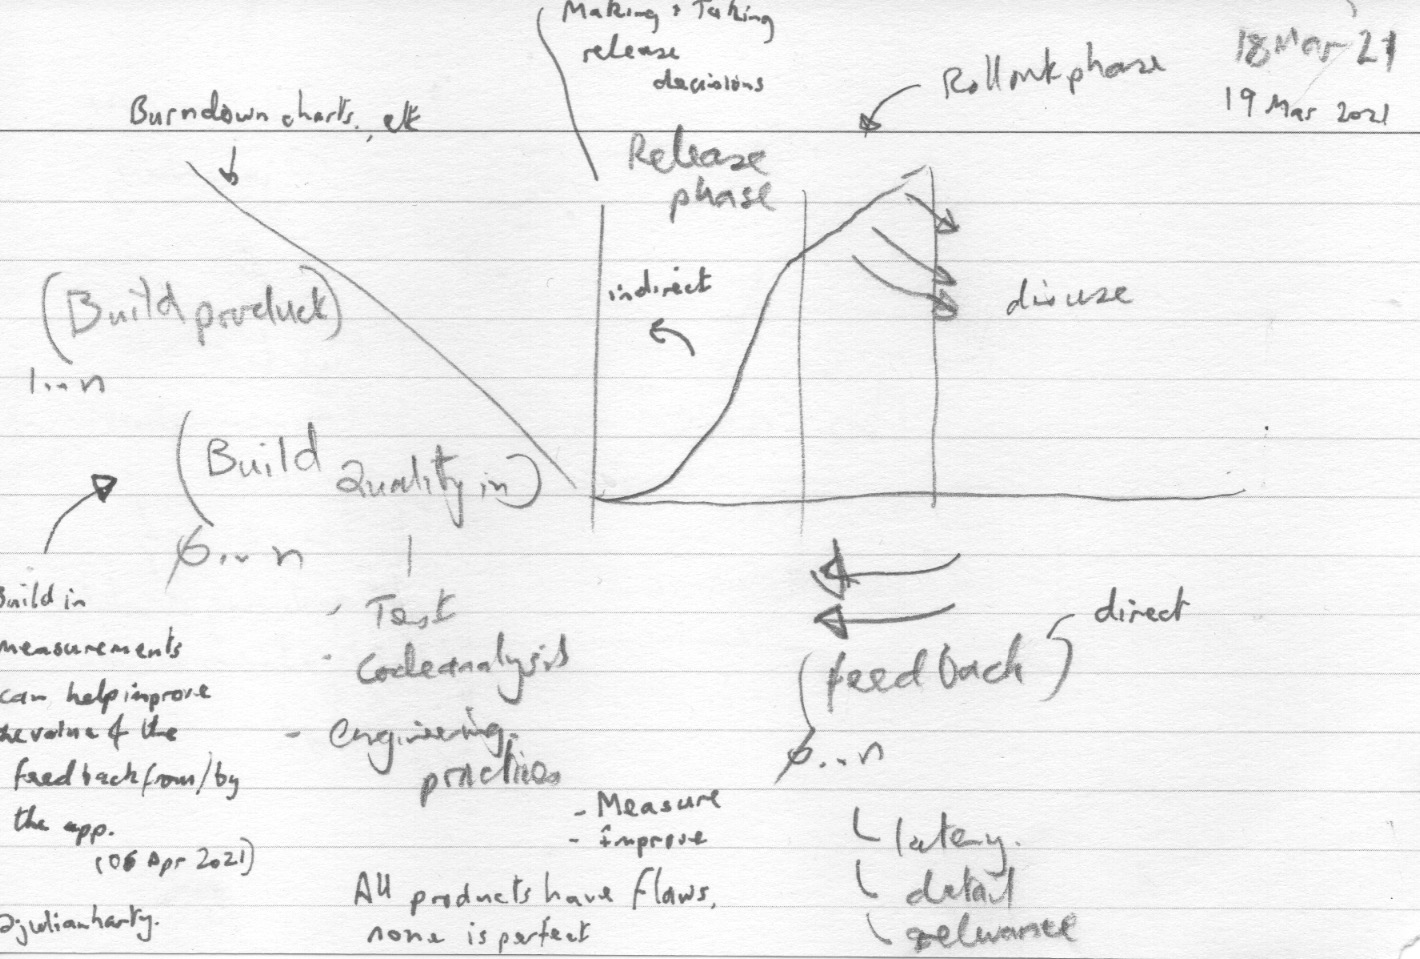
\includegraphics[width=15cm]{images/rough-sketches/Red-Thread-Rough-Sketch.jpeg}
    \caption{The lifecycle of a release and where mobile analytics provides feedback}
    \label{fig:red-thread-for-this-thesis}
\end{figure}

For any given release of a mobile app there are at least three material phases in order for the release to be used:
\begin{enumerate}
    \item Building the product: which may incorporate practices and tools intended to ship a `quality product'. Some teams also incorporate logging and reporting to help measure the behaviours of the app in use, post release.
    \item The Release: For some projects this may be as simple as uploading a new binary and making it fully available. For others they may incorporate decisions and mechanisms to make each release with the aim of de-risking any undesirable/adverse effects of the new release.
    \item Deployment: Deployment occurs when end users install and start using the release of the app. Both the app store and the end users affect when this occurs. App developers can try to hasten when users install the latest release through various mechanisms, for instance through implementing and mandating users upgrade their current release.
\end{enumerate}

Figure~\ref{fig:red-thread-for-this-thesis} illustrates these three phases together with some of the dynamics \emph{e.g.} of rollout and disuse of a release, and of feedback from whatever sources that the development teams can choose to pay attention to and apply. These phases are part of a longer lifespan of the release that includes an often long-term postdelivery period~\citep[pp 156-157]{evans2004_achieving_software_quality_through_teamwork} where users use the release until it is decommissioned or replaced with a subsequent release.

\begin{figure}
    \centering
    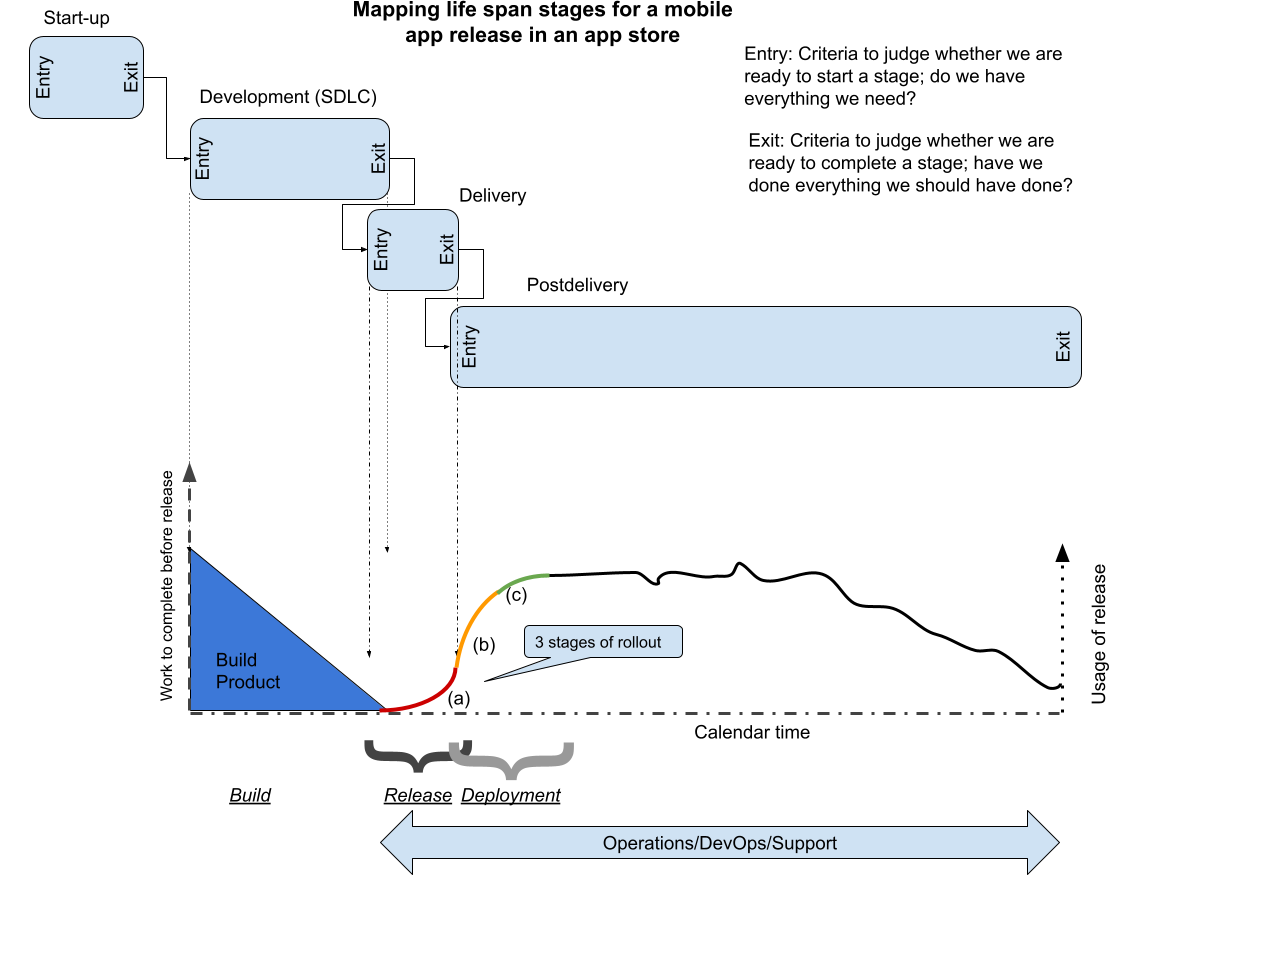
\includegraphics[width=16cm]{images/my/mobile-app-life-span-stages.png}
    \caption{Mapping life span stages for a mobile app release in an app store}
    \label{fig:mobile-app-life-span-stages}
\end{figure}

Figure~\ref{fig:mobile-app-life-span-stages}~\footnote{Source of figure, Google Drive file: \href{https://docs.google.com/document/d/1d4B5l1tlpclHdKwY8W00qchiCV2YK5JjJP8TbkRHcjQ/edit}{Mobile app life span stages}.} compares a revised version of the `Life span stages' Figure in~\citep[p.155]{evans2004_achieving_software_quality_through_teamwork} mapped approximately to the three stages first illustrated in Figure~\ref{fig:red-thread-for-this-thesis}. Mobile app releases in an app store extend the Delivery which may also overlap either or both the development and the postdelivery life span stages. The overlap with the development stage is because the development is not complete until the app store accepts/approves the release (this may include pre-launch checks, automated testing, and so on depending on the app store). The overlap with deployment happens as releases are often released incrementally initially to a small percentage of the userbase - at least some of the users in that percentage will install the new release, until the percentage has been achieved. Meanwhile at least some of those users will use the app which will then mean the release is operational and may need operational support.


This research found that developers are able to materially improve the stability/reliability~\footnote{For Android Google used the term `stability' when they describe their Android Vitals service which is incorporated into Google Play Console. It effectively measures reliability for two specific types of failure: crashes and ANRs. An overview of Android Vitals is available online from various Google and Android sources including~\citep{android_vitals_overview_2019, android_vitals_best_practices}. HP also used the term `~\href{glossary-stability}{stability}' to measure crashes in mobile apps.}
%
of their mobile apps when they use the results of mobile analytics to assess the stability/reliability, identify groups of failures, triage the failures, and address the ones they decide to action. Where project teams stop paying attention to this process the failure rate increases of their new releases - the apps tend to entropy and failure.

Diligent developers and development teams can materially improve the stability/reliability of their apps through applying good coding, design and architecture patterns. Even these practices do not guarantee the releases will always be trouble-free. By paying ongoing attention to analytics during development, testing, and the rollout of releases flaws can be identified before the release reaches the majority of the userbase and teams can ameliorate the effects of many of the flaws.
\clearpage 


\section[A framework for applying mobile analytics effectively]{A framework for applying mobile analytics effectively\\ \small{(Possibly integrate into: Applying analytics to development practices?)}}

\marian{The conceptual prerequisite tree is unclear. She observed it has 2 threads of enquiry; Do the boxes have the same magnitude etc.?}

\textit{I clarified the prerequisites are prerequisites to effective application of mobile analytics. The figure is of a framework either corroborates or revises the approach. It could become an actionable list. Each item identifies a potential points of failure. Or it could be used as a retrospective of the factors I observed. It could be used to reflect on practice. It breaks the topics down.}


The lived experiences of participating in the various case studies, together with the results and insights gleaned from them, led to the development of a potential framework for the successful and effective application of using mobile analytics to improve the reliability of the app. These are illustrated in Figure~\ref{fig:using-toc-cpt-using-mobile-analytics-to-improve-mobile-apps}~\footnote{Source of figure, Google Drive file:  \href{https://docs.google.com/document/d/16PaSFRVzg1b2Nykly8qzaTAHtJqtEwgrK754wuek53M/edit}{2021 Applying Theory of Constraints to using Mobile Analytics to improve Mobile Apps} - which needs to be further revised.}. It is based on a diagram known as a conceptual prerequisite tree which is part of Eli Goldratt's Theory of Constraints\footnote{(applying Theory of Constraints, see~\citep{goldratt2017_necessary_but_not_sufficient, lepore1999_deming_and_goldratt, scheinkopf1999_thinking_for_a_change})}. 

Each item is essential in order to \emph{actually} apply mobile analytics in order to improve the quality of mobile apps, \emph{i.e.} they need to be adequately satisfied. Satisfied != perfection. There are other complimentary ways to improve the quality of mobile apps, for instance through designing and implementing automated tests that exercise subsets of the code. Failures reported by mobile analytics are concrete \emph{i.e.} the developers now know the code fails in some circumstances which may motivate the developers to write targeted automated tests. Several of the case studies included developers writing such tests. 

\begin{figure}
    \centering
    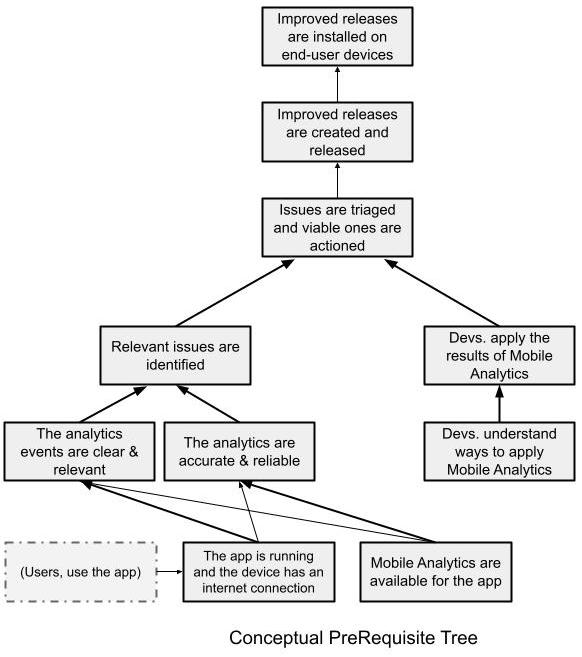
\includegraphics[width=11cm]{images/my/Conceptual_prereq_tree_Applying_Theory_of_Constraints_to_using_Mobile_Analytics_to_improve_Mobile_Apps.jpeg}
    \caption{Conceptual Prerequisites Tree: Using mobile analytics to improve mobile apps}
    \label{fig:using-toc-cpt-using-mobile-analytics-to-improve-mobile-apps}
\end{figure}



%
The underpinnings in terms of being able to improve mobile apps are threefold: 
\begin{enumerate}
    \item Users need to use the app. The app's behaviours will include errors and failures.
    \item The app needs connectivity together with at least one form of mobile analytics.
    \item Developers need to understand the outputs of mobile analytics and address pertinent issues in future releases of the app.
\end{enumerate}

An expanded list of the prerequisites illustrated in Figure~\ref{fig:using-toc-cpt-using-mobile-analytics-to-improve-mobile-apps} is as follows (roughly in descending order. Analytics data from previous releases is used to help improve \emph{future} releases.

\Prerequisite{Essential prerequisites to improve the reliability of apps using mobile analytics}
{\small
\begin{enumerate}
    \itemsep0em
    \item Users use the app
    \item Improved releases are in-use on end-user devices
    \item Improved releases are installed on end-user devices
    \item Improved releases are created and released
    \item Analytics logging refined to capture relevant information
    \item Issues are triaged and viable ones actioned
    \item Devs have adequate, timely access to mobile analytics outputs
    \item Devs apply the results of mobile analytics outputs
    \item Devs understand ways to apply mobile analytics
    \item Relevant issues are identified and analysed
    \item The analytics service is accurate and reliable
    \item The analytics events are clear and relevant
    \item Volumes of data do not overwhelm system or devs
    \item The app is running and the device has an internet connection
    \item Mobile analytics are available for the app
    \captionof{prerequisites}{Prerequisites to improve the reliability of apps using mobile analytics}
    \label{prerequisites-essential}
\end{enumerate}
}


\Prerequisite{Additional, desirable prerequisites}
In addition to the essential set of prerequisites, in ~\ref{prerequisites-essential}, the following are also highly desirable:
{\small
\begin{enumerate} [i]
    \itemsep0em
    \item Ecosystem is adequately and acceptably secure
    \item System is performant
    \item System is unbiased
    \item Internally and externally verifiable system and service
    \item Users have practical controls on the data processed
    \item Available data sufficiently representative to apply to the population
    \item Current and historical data and reports seamlessly available to development team
    \captionof{prerequisites}{Additional, desirable prerequisites when using mobile analytics}
    \label{prerequisites-desirable}
\end{enumerate}
}

\subsection{When can identified issues be addressed?}
To address issues they need to be identified and a practical improvement determined. The practical improvement may be an outright fix, or a workaround, or an amelioration, etc. The questions for the development team include where and when the improvements can be applied to improve the reliability for the end users of their app.

Some issues can be ameliorated externally to the app, for instance though changes to servers that support API requests from apps, however many need changes to the app in order to be effective.

For apps released as compiled binary files (the vast majority in iOS and Android app stores), improvements are generally made to a subsequent release than the one(s) where the failures have been occurring\footnotemark. And these subsequent releases need to be installed by the user population and used similarly in order to determine whether the improvements were worthwhile. Some users keep older releases and others stop using the app so 100\% rollouts of subsequent releases are not practical. (For apps that only ever had one release then 100\% rollout is \emph{de-facto}.)

\footnotetext{
  There are various ways that a binary \emph{can} be patched or updated \textit{in-situ}. Indeed various security attacks are performed using this approach, as, for instance,~\citep{poeplau2014_execute_this_unsafe_android} discussed. Around April 2013 Google changed their policy for Google Play to forbid Android apps from modifying, replacing or updating it's own APK binary code outside Google Play's update mechanism (the policy is still available on the Internet Archive Wayback Machine~\href{https://web.archive.org/web/20130426113437/https://play.google.com/about/developer-content-policy.html}{Google Play Developer Program Policies}). In 2019, Google provided developers with an API that developers can embed into their Android app in order to prompt users to update the app using Google Play~\citep{android_in_app_updates}. 
}

\newthought{Would time-machines help?}
If time-machines were available in software development developers might be able to go back in time and repair the current application on the user's mobile device before it was installed on the device. 

Conversely, a time-machine could enable users to return to the time and context when an event such as a failure occurred in order to help the developers understand contributory factors that led up to the failure and the aftermath. 

\newthought{Prior art in time-machines}
\textit{FYI This will be moved to the Related Work chapter}
In 1999, time-machine computing was introduced as a way to help to organise and manage electronic information in computing environments, for instance using a desktop environment - `TimeScape' - that supported time travelling on the computer, and time-casting to restore the context that surrounded the use of a given application~\citep{rekimoto1999_time_machine_computing}. However, that work was limited to a desktop computer environment and has not been maintained. 

\newthought{Breadcrumbs preserve history}
Some mobile analytics libraries include support for breadcrumbs (event records)~\citep[p.683]{MacLean2015_pro_android_5_book}; these breadcrumbs can augment the crash data by providing a recorded history of the events that occurred in the app before the crash happened. The recorded history can help the developers perform \emph{post-hoc} analysis of events that preceded the crash failure. 

\newthought{Record and replay/playback}
Recreate the `journey' (however relevant context may be missing or different and therefore affect the results and conclusions). Various reasons why recreating the journey is desirable e.g. to reproduce failures to help understand their characteristics and causes, to learn indirectly by observing and visualising the journey. \emph{c.f.} heatmapping. Record and replay offers the possibility of moving beyond using breadcrumbs as it is intended to record sufficient information to reproduce the use of an app. However there are various limitations in the tooling, the techniques, and at least as importantly the unacceptability of recording end user sessions on their devices using production releases of apps downloaded from the app store. 

\newthought{Prior art in record and replay/playback}
\textit{FYI This will be moved to the Related Work chapter}
TBC

% [4] Joorabchi, Mona Erfani, Ali Mesbah, and Philippe Kruchten. "Real challenges in mobile app development." Empirical Software Engineering and Measurement, 2013 ACM/IEEE International Symposium on 10 Oct. 2013: 15-24.~\citep{joorabchi2013_real_challenges_in_mobile_app_development}

\clearpage
\section[Socio-technical aspects]{Socio-technical aspects\\ \small{(Probably cover this topic in the Discussion and the Conclusion.)}}
\buzzwords{Systems Thinking, Games people play}

\emph{Note: the current thesis doesn't have much on this topic. TBD whether to include it, it's certainly pertinent in my view. Tip: don't use the term Game Theory as I'm not going to establish, test, or evaluate the case studies using an actual theory.}

Many developers fail to address all the issues identified through use of mobile analytics and a key influence is their perceived ability to successfully address issues identified by the analytics. Furthermore, these issues are collectively only one of many demands for their time and attention. Human, organisational, and business factors all influence the extent mobile analytics is a) used and b) the results addressed. This research touches on both the mechanics of applying mobile analytics together with the `game' which are the higher-level human nature aspects which affect the application and the value of applying the mechanics. Figure~\ref{fig:the-mechanics-the-game} provides a simple illustration of the game and the mechanics.

\begin{figure}
    \centering
    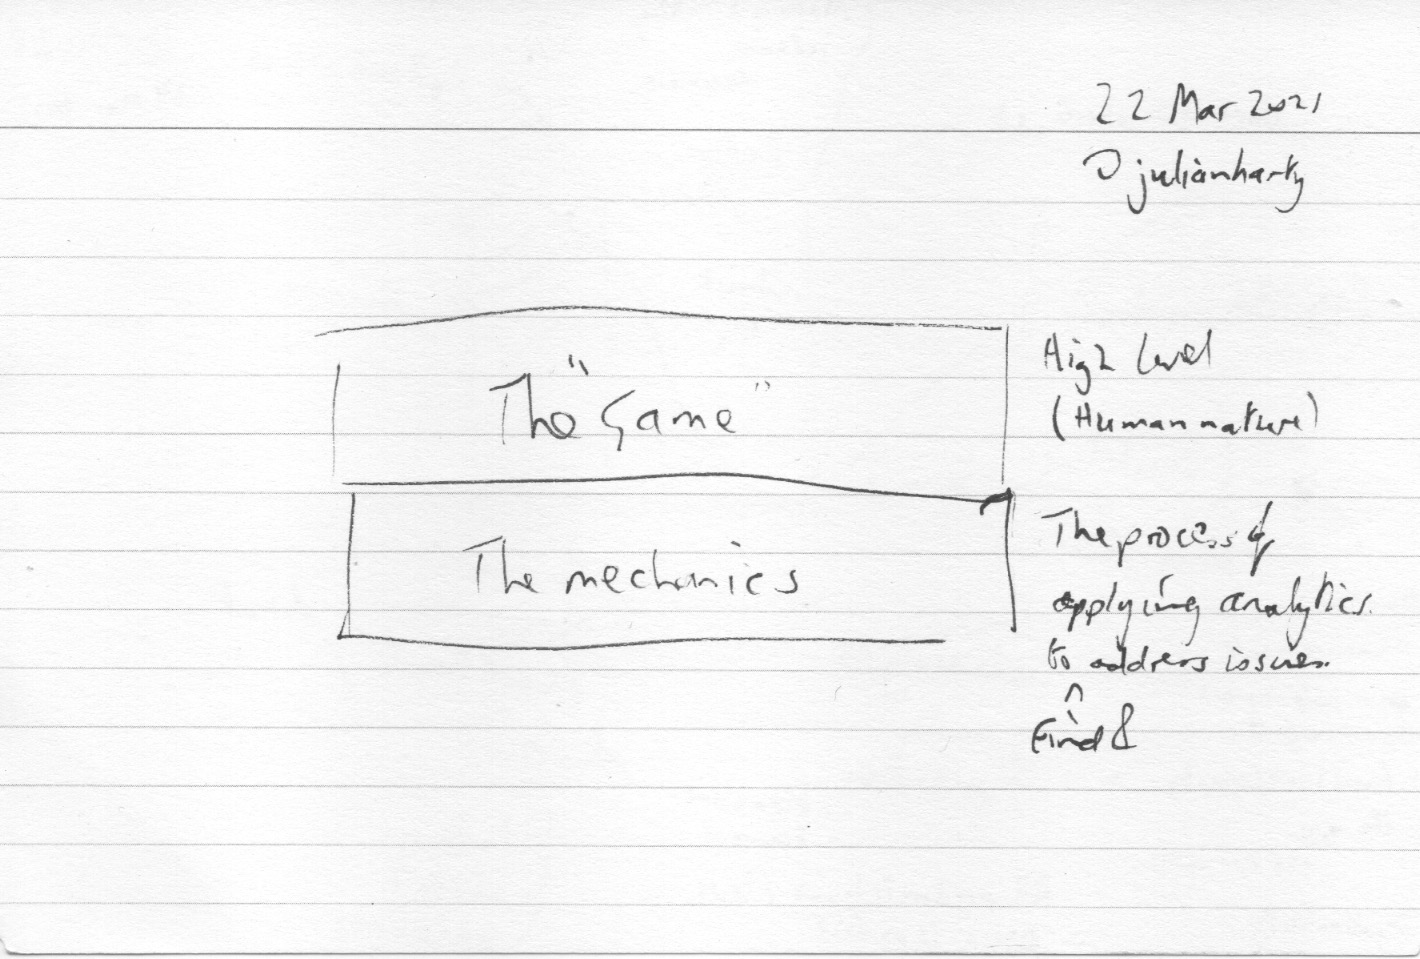
\includegraphics[width=15cm]{images/rough-sketches/The-Mechanics-The-Game.jpeg}
    \caption{The Mechanics and The Game of using Mobile Analytics}
    \label{fig:the-mechanics-the-game}
\end{figure}


\newthought{Living with risks} 
Risks include the risks of not using analytics and the risks of using analytics. Risk taking and risk aversion on the part of the developer, the team, the organisation, the app store organisation, and the end user come to play in the game.

Given the ongoing examples of misdeeds and corruptions in the application of data collected from user's activities and user's content - understanding and analysing the \href{glossary_data_dynamics}{[data] dynamics} of the information gathered, processed, and transferred in support of mobile analytics is also pertinent.

\newthought{Effort and rewards}
Significant data is available for minimal effort; paradoxically the lack of effort may lead to some developers underestimating the usefulness of using this data.

Development teams who choose to invest in analytics are able to reap better and more relevant results. Developers can choose to augment platform-level analytics with in-app analytics to augment or supersede aspects of what the platform provides.

\newthought{Risks and choices}
Developers can choose when they will pay attention to the analytics; they can also choose the extent they wish to integrate analytics into their apps. 

There are risks and responsibilities of the effects of collecting data and performing analysis on that data, practices outstrip legislation. It remains possible for sensitive findings to be discovered through the use of mobile analytics, nonetheless the ethical challenges are not unique to mobile analytics~\footnote{Arosha mentioned \href{https://www.orbit-rri.org/}{ORBIT-RRI} and their ~\href{https://www.journals.elsevier.com/journal-of-responsible-technology}{Journal of Responsible Technology}. There are various areas that overlap and potentially align in their concepts, I've not found much relevant concrete material yet, this footnote is a reminder (it is not intended to be part of my thesis.}.

\newthought{Freedom and responsibility}~\label{newthought-freedom-and-responsibility}
Developers often have more freedom in relation to how an app behaves than the users of their apps do. In practice the vast majority of Android apps in Google Play use and collect mobile analytics, the only material choice the users have is whether to use or not use a particular app. Sometimes the freedom is to \emph{not make a decision} (as mentioned earlier). Making a decision may have consequences. Not making a decision may have consequences. 

Who gets to choose may also be influenced by the larger organisation developers belong to. For example, in some large enterprises developers of an individual app may have to use prescribed mobile analytics rather than being able to make an independent [informed] choice.


\newthought{Minimise harm maximise value address material known issues}~\label{newthought-do-no-net-harm}
In the field of doctors there are discussions by \citealt{Schuenemann2011_guidelines2_0_do_no_net_harm} and \citealt{Sokolf6426_2013_first_do_no_harm_revisited} on \emph{do no net harm}. This has been eloquently adapted to \emph{``A competent and caring physician is one who never causes unintentional or unnecessary harm.", Stephen Ross Workman, MD}~\url{https://www.bmj.com/content/347/bmj.f6426/rr/671112}. Implicitly it could also apply to what users expect from the mobile apps they install and use. So, perhaps a the concept could be extended to the following maxim?: \emph{an app developer not only never causes unintentional or unnecessary harm, they also strive to address whatever harms do affect the users of their apps while also satisfying for other demands}~\footnote{In medicine there have been similar discussions on freedom and responsibility, and in particular on aftercare of what they publish~\citep{rennie1998_freedom_and_responsibility_in_medical_publication}.}.

MUST-DO expand on~\citep{shklovski2014_leakiness_and_creepiness_in_app_space_perceptions_of_privacy_and_mobile_app_use, zhou2017_user_perceived_control_trust_etc_smartphone}.

\textbf{MUST-DO} Explore these themes in the Discussion chapter. Consider separating: 1) those supported by primary evidence in the case studies (a subset of the experiences from the field, some evidence is protected by confidentiality agreements, etc.), 2) those more speculative in nature/based on literature and hence topics for further research.

\isabel{Ask Fiona Charles about her ethics for software engineers}

\clearpage
\section[Practical aspects of using analytics]{Practical aspects of using analytics \\ \small{(Possibly migrate to the Conclusion? else the Discussion?)}}
Analytics providers have a major influence on the efficacy of the application of mobile analytics. There are limitations and flaws in the various tools this research has encountered regardless of their source (\emph{e.g.} in-house proprietary, opensource, free and paid-for commercial proprietary offerings). Nonetheless, flawed offerings are still able to be used to deliver improvements in the mobile apps. Specialised startups such as Iteratively aim to increase the coherence of embedded analytics (those embedded into the apps) while also increasing compliance. HP's AppPulse Mobile provided no-code analytics for mobile apps where their tools automatically instrumented the binary to add the analytics; several providers offered GUI interaction recording and `heatmaps' generated using aggregated recordings of touch screen interactions.

Those who applied the results of mobile analytics were able to increase the stability/reliability of their mobile apps. The amounts of improvements varied based on various factors such as:
\begin{itemize}
    \itemsep0em
    \item The starting point for the app.
    \item The amount of ongoing engagement of the development team.
    \item The choices of mobile analytics services and the use of proactive event recording using the related analytics libraries.
    \item The sources and causes of some of the issues being reported - some where far harder to diagnose than others, and several originated outside the actually codebase of the mobile app where it might be impractical to truly fix the source of the issue.
\end{itemize}

\noindent
\rule{\textwidth}{0.4pt}

\clearpage
\section{Where's my current focus?}
It's in several areas:
\begin{itemize}
    \item Create a presentation to sum up the research.
    \item Provide coherence and consistency to the empirical studies. Learn about methodologies applied to empirical studies.
    \item (Ongoing) Some additional development of the possible framework in Section 0.6 and Figure 0.3
    \item (Ongoing) On the related work chapter, adding various references and starting to develop these into coherent discussions of these works, the gaps in research, etc.
    \item (Done) To revise the red-thread for the case studies and create three distinct tables as per my discussion with Marian and then flesh out and organise the case studies.
\end{itemize}



\begin{comment}
\chapter{Introduction}
\label{the-introduction}
% This should cover the problem the thesis addresses, the aims and questions, the thesis structure, a summary of the main findings and a discussion on the thesis' contribution. It should prime the reader for what's about to come by providing an overview of what lies ahead.

% Establish your research territory by situating your research in a broader context. 
% Establish and justify your niche by describing why your research is needed. 
% Explain the significance of your research by describing how you conducted your research.
Billions of people use mobile apps on two main mobile platforms Google Android and Apple iOS and their related operating systems, and Android is integrated into additional mobile platforms including Kindle OS and various Chinese manufacturer's ecosystems, particularly Huawei with HarmonyOS. There are millions of these mobile apps developed by millions of developers across the globe. Failures in these apps can adversely affect the experiences of end-users, businesses who provide apps, and/or goods and services through mobile apps. 

This thesis focuses on the most used operating system - Android - in it's most popular and mature platform - Google Android - to discover whether mobile analytics can help the developers improve the stability of their apps. 
%
Stability is a prerequisite for an app to be viable in the marketplace and several key app stores clearly state unreliable apps~\emph{e.g.} apps that crash, will be marked down and possibly ejected from the app store~\citep{appleappstore2021_app_completeness, google_play_policy_center_broken_functionality, huaweidevelopers_appgallery_review_guidelines}. Apple states~\emph{``On average, over 40\% of app rejections are for Guideline 2.1 – Performance: App Completeness."}~\citep{appleappstore2021_review_avoiding_common_app_rejections} with crashes and debugs listed as the first rejection reason. Crashes are undesirable and commonplace therefore one of the key software qualities in use where analytics may be able to help measure and improve reliability for end users. 
% See also a developer's question about releasing iOS apps with known crashes https://developer.apple.com/forums/thread/68770

Furthermore, even leading technology companies release software that crashes, some have the misfortune to release software that crashes other apps inadvertently as Google discovered in Spring 2021~\citep{bbcnews2021_google_fixes_crashing_android_app_issues}. And App developers, including the BBC for their iPlayer app, posted advice to end users on the issue in Google Play~\citep{bbc_iplayer_app_april_2021_webview_information}.

An increase in crashes led to an increase in `churn'~\footnote{Churn is also known as attrition and is used to measure users who leave a collective group over a specific period~\url{https://en.wikipedia.org/wiki/Churn_rate}.} according to an industry report of up to six times the average rate of churn~\citep{levy2016_crash_and_churn_report, levy2017_the_crash_and_burn_report_findings}~\footnote{Note: Apteligent was acquired by VMWare in 2017 and few of their online materials remain available.}. % A counter point is that a few organisations can survive crashes in their app, for instance Facebook according to https://9to5google.com/2016/01/04/facebook-intentionally-made-its-android-app-crash-to-test-how-addicted-users-are/ However this is not likely to be the norm for other app developers who lack the scale and pull of Facebook's platform.

Conversely, Android apps that score highly in terms of stability may be selected to be promoted and featured in Google Play. One of the developer-oriented Google Play Guides provides an imperative: `Improve your app’s quality and discoverability'~\citep{android_store_listing_guide} which combines with the Google Play Guide on Android Vitals. This states~\emph{``Apps whose metrics are higher have greater promotability, which raises their ranking in Google Play Store searches. They also are more likely to be eligible for the New \& Updated and Editor's Choice collections on Google Play, and to be nominated in the Google Play Awards."}~\citep{android_android_vitals_guide}. % See also https://blog.embrace.io/top-5-reasons-your-app-is-losing-discoverability-on-google-play-store/

A default mobile analytics service is integrated into the Google Android platform and available free of charge for all developers of apps in the Google Play App store so it was selected as the default analytics tool for this research as it is prevalent, widespread, and also one of the quality signals Google uses to decide whether to promote apps in their app store. The default mobile analytics service is complemented with research in additional analytics tools to provide perspective and contrast in their various characteristics and capabilities.

\yijun{Should talk about quality (echoing the title), then talk about reliability and other quality issues.}
% https://developer.android.com/docs/quality-guidelines/core-app-quality
\citep{android_guidelines_core_app_quality}

\begin{comment}
    Mobile-app quality is becoming an increasingly important issue. These apps are generally delivered through app stores that let users post reviews. These reviews provide a rich data source you can leverage to understand user-reported issues. Researchers qualitatively studied 6,390 low-rated user reviews for 20 free-to-download iOS apps. They uncovered 12 types of user complaints. The most frequent complaints were functional errors, feature requests, and app crashes. Complaints about privacy and ethical issues and hidden app costs most negatively affected ratings. In 11 percent of the reviews, users attributed their complaints to a recent app update. This study provides insight into the user-reported issues of iOS apps, along with their frequency and impact, which can help developers better prioritize their limited quality assurance resources. source:\citep{khalid2015_what_do_mobile_app_users_complain_about}
\end{comment}

\begin{comment}
    In the mobile-app ecosystem, user ratings of apps (a measure of user perception) are extremely important because they correlate strongly with downloads and hence revenue. A case study examined the relationship between ratings (and the associated review comments) and static-analysis warnings (collected using FindBugs) for 10,000 free-to-download Android apps. Three warning categories - bad practice, internationalization, and performance - were more frequent in low-rated apps and corresponded to the review comment complaints. Thus, these categories were closely related to the user experience. These results suggest that app developers could use static-analysis tools to identify the bugs behind the issues that users complain about, before releasing an app. source:~\citep{khalid2016_examining_the_relationship_between_findbugs_warnings_and_app_ratings}
\end{comment}

\begin{comment}
    App Store Analysis studies information about applications obtained from app stores. App stores provide a wealth of information derived from users that would not exist had the applications been distributed via previous software deployment methods. App Store Analysis combines this non-technical information with technical information to learn trends and behaviours within these forms of software repositories. Findings from App Store Analysis have a direct and actionable impact on the software teams that develop software for app stores, and have led to techniques for requirements engineering, release planning, software design, security and testing. This survey describes and compares the areas of research that have been explored thus far, drawing out common aspects, trends and directions future research should take to address open problems and challenges. source:~\citep{martin2017_survey_in_app_store_analysis_for_software_engineering_IEEE_edition}
\end{comment}

\begin{comment}
    In this paper, we study the app store as a phenomenon from the developers perspective to investigate the extent to which app stores affect software engineering tasks. Through developer interviews and questionnaires, we uncover findings that highlight and quantify the effects of three high-level app store themes: bridging the gap between developers and users, increasing market transparency and affecting mobile release management. Our findings have implications for testing, requirements engineering and mining software repositories research fields. These findings can help guide future research in supporting mobile app developers through a deeper understanding of the app store-developer interaction. source:~\citep{alsubaihin2019app_store_effects_on_software_engineering}
\end{comment}

As Febrero, Moraga and Calero note~\emph{``Software Quality is a multidimensional concept for which Reliability is considered as a key attribute."}~\citep{febrero2017_software_reliability_as_user_perception}.

Broadly, the research is to understand whether mobile analytics can help developers to improve the reliability of their apps. A second applied research area emerged as various flaws and limitations were discovered in the various mobile analytics services, to discover and categorise the flaws and limitations, and to consider some of the effects of these flaws and limitations. 

In the research developers were able to improve the measured reliability for each of the case studies despite the flaws and limitations. Some improvements were gained with small amounts of effort, others were performed through more strategic changes including replacing Java code with Kotlin replacements and retiring buggy modules and external libraries.  

\begin{comment}
    \begin{itemize}
        \item Get the audience to identify with someone or something, - Give that someone or something some kind of need, - And start changing the circumstances.
        \item Have that someone or something deal with the new circumstances - And find the thing that was needed.
        \item Have that someone or something pay the price of the find - And start heading back toward the original circumstances.
        \item show how those original circumstances have changed as a result.
    \end{itemize}
    \emph{Dan Harmon's story telling circle}
\end{comment}



\section{Ontology and Epistemology}
Before going into details, I will introduce the basis for my theoretical perspective in terms of the ontology and epistemology.~\footnote{
\begin{itemize}
    \item Ontology \( \rightarrow \) a theory of `being' (existence).
    \item Epistemology \( \rightarrow \) what we can know about the microcosm/the world and how we can know it (a theory of knowledge).
\end{itemize}

Both these terms are taken from~\cite{marsh2002skin}. While the article is aimed at social science research, it introduces both topics and their relationships clearly and practically~\footnote{Note: newer versions of the introductory material is published in a book: \href{https://www.macmillanihe.com/page/detail/Theory-and-Methods-in-Political-Science/?K=9781137603517}{\emph{``Theory and Methods in Political Science (\nth{4} Edition)".}}}.
}

\subsection{Ontology}
Analytics exist and are used across and throughout software development practices. Software is not perfect, it's formed through numerous human endeavours using flawed tools and techniques. No practical software is bug-free, nonetheless those involved can improve software through their choices and practices.

[Almost] anything can be measured sufficiently to be useful. In (\cite{hubbard2014measure}) \emph{How to measure anything, \nth{3} edition} the author argues that anything can be measured and proposes an approach to do so. His framework, called \emph{Applied Information Economics: A Universal Approach to Measurement} is summarised in five steps:

\begin{enumerate}
    \item Define the decision.
    \item Determine what you know now.
    \item Compute the value of additional information. (If none, go to step 5.)
    \item Measure where the information value is high. (Return to steps 2 and 3 until further measurement is not needed.)
    \item Make a decision and act on it. (Return to step 1 and repeat as each action creates new decisions.)
\end{enumerate} %~\cite{hubbard2014measure} (page 9).

This approach helps to frame this research into applying analytics to development practices, especially in terms of the practical aspects and nature of real-world apps, development teams, and user-bases..

\subsection{Epistemology}
Here we consider the questions: (1a) What we can know about mobile analytics and (1b) how we can know it? Then more specifically, these related questions are key given this research focuses on using mobile analytics to help answer the next question. (2) How we know about the identification and measurement of some flaws in behaviour of software that are considered measures of quality of the software in use? Broadly we can learn from people, use software tools, and use data to answer these questions. In some cases the data comes from a single source, in others cases from several.

\textbf{Toolbox of methods, how can we know about mobile analytics and the effects of using them?} 

Mobile analytics comprises software, systems, and sometimes services. Broadly we can read about them, study their source code, analyse, test, and use them directly, and ask others for their perspectives and insights. Rather than go into lots of detail here, several of the appendices of this thesis cover aspects of mobile analytics, in particular, in~\href{chapter-on-mobile-analytics}{\emph{\nameref{appendix-on-mobile-analytics}}}. 

In terms of learning from people, we can do so by asking the designers, constructors, operators, and users of a system. However, we're also limited by who we can ask, what they are willing/able to communicate, and whether that communication is sufficiently open and transparent to be useful and reliable. We can also learn from information produced by people, and in particular for mobile apps we can use ratings and reviews. Given human behaviour it may also be worth considering aspects such as the provenance of the information sources, fake data, \emph{etc.} especially where there are rewards for slewing the results of the measurements being used in an ecosystem. 

We can know through static analysis tools, automated tests, end-to-end testing, \emph{etc.} and all of these are used by at least some of the developers of mobile apps some of the time. They often take place \textit{before} the software is released to end users.

We can also know through data collected when the software is used. As~\cite{RFC3164} notes in RFC3164, ~\emph{``Since the beginning... operating systems, processes and applications were written to send messages of their own status, or messages to indicate that certain events had occurred. These event messages generally had local significance to the machine operators."}. Mobile apps also write messages locally and developers use them for similar purposes (nuances and differences are discussed in the related work chapter). These local messages can be read by humans locally and/or read by software that delivers them elsewhere. Developers can also add software to their apps to log information for processing elsewhere which is where much of mobile analytics and crash reporting fits in the scheme of things.

Log messages are written locally on the same device (\textit{i.e.} computer) that runs the software. When developers are developing the software they tend to be local to the device and therefore able to read the logs. When the devices are remote, as they are for end users of mobile apps, developers cannot easily access the logs or read them. If they wish to do so they need mechanisms to obtain the logs. They can choose to incorporate mechanisms into the app including custom logging mechanisms that transmit the logs so they can be processed remotely. They can rely on log forwarding software~\footnote{For instance a fairly involved example for Flutter Android apps, using MQTT, is described in~\citep{adil2020_sending_logs_from_flutter_apps}}, and/or mechanisms provided on the device if they exist. 
% A couple of Android implementations for LogStash include:
%  https://github.com/Labgoo/android-logstash-logger
%  https://gist.github.com/PatrykGala/55603fe4259d812fdc0ffbc9e63eaabc (saved in my references)


Various data can be potentially collected implicitly and explicitly. What can be collected depends on the observation mechanisms. Observation may be within an app or external to it, for instance by the operating system as both iOS  and Google Android do~\footnote{There are other custom versions of Android, for instance used in Amazon Kindle Fire devices. Their details are outside the scope of my research.}(details in the Appendix titled~\href{chapter-on-mobile-analytics}{\emph{\nameref{appendix-on-mobile-analytics}}}). Within an app the observation may focus at a single layer, for instance the visual user interface, or several. The choices of observation mechanisms within an app are made by developers or their stakeholders. The choices external to an app can be made by various people including the platform provider, users, or indirectly using other software including third-party apps, spyware, accessibility software, and so on.

Analytics, such as user-journeys, can help to answer questions about the usage of the software. They help establish \emph{what-is}. As we understand more about what-is we can then consider \emph{what-would-be-better} and do gap analysis between what-is and what-would-be-better.

Reporting/generating and Observing... What happens within the app stays within the app unless someone looks inside the app or the app reports what's occurring. Observation without action limits the utility of whatever is learned. 

Survivorship bias (\cite{wikipedia_survivorship_bias}) is relevant to understanding the information developers receive, some data does not `survive' the journey from source to developer. And much of the information that is does reach the developers does not survive or, perhaps better put, thrive in terms of being used productively. They have plenty of other demands for their time and attention and much of what could be useful isn't used in practice, therefore the data needs to be sufficiently useful and relevant and improvements tractable for any proposed approach to be used long term in practice.



\section{The Research}
Software app developers need to deliver software that can be used successfully by end users. To do so they need to be able to create software and distribute it so it is available to end users. They need to do so in a timely manner, and perfection may be too long to wait for. End users need to be able to install and use that software. If the software is sufficiently usable, useful and behaves adequately they may continue to use it. Developers cannot assess \emph{a priori} whether their software will meet the needs and expectations of users, meet their needs, or the needs of their stakeholders. In short they do not know whether it will thrive.

One of the key considerations is whether the quality of their apps are adequate. There are many ways to assess quality of apps, including static analysis, in-person testing, and automated testing. Users may perform their own subjective assessments of quality and some of these users provide feedback in the form of ratings and reviews. 

Researchers have investigated these various sources of quality related information. My research concentrates on using sources of analytics related to usage of apps to help developers a) assess the quality of their current software, and b) improve the quality using the same analytics sources.

This research was inspired by learning about the power and capabilities of applying usage data collected by mobile apps in extremely popular real-world mobile apps in the early days of mobile apps (before Android, iOS and other modern mobile platforms were released). At the time I worked for Google and was responsible for testing all Google's mobile apps, including: Search, GMail, Maps, and many others.

Several years later, when consulting with another company with over ten million active users I discovered they had included two analytics tools in their apps where there were numerous discrepancies in the data collected, the ways the counted and the resulting reports, yet they were both considered necessary. The engineers then added a third analytics library in the hope it would correlate with one or other of the existing libraries - it didn't, instead it had distinct characteristics and counts. And yet the developers were able to discover how their apps were used in incredible detail and by applying what they learned their apps became increasingly popular and financially successful.

These experiences led me to starting my PhD in order to research the potential of mobile analytics, and to understand some of their flaws and the effects of those flaws. During my research there have been incredible changes in the mobile landscape (for instance major manufacturers, operating systems, etc. have appeared, mushroomed, and disappeared). Similarly many test automation tools and frameworks have been and gone. Meanwhile, apps and app stores have spread beyond smartphones and tablets to desktop operating systems, cloud-based product offerings such as Salesforce, etc. Google's Android platform includes platform-level data collection, reporting and analytics intended to help developers learn about ways they can improve their apps. Meanwhile regulation has started to emphasise and highlight some of the many risks and concerns with gathering data wantonly. 

Despite all these changes, and my limited inroads into a subset of the entire landscape, the research seems to indicate the potential of applying usage analytics to improve both the product (the software) and the process (how the software is developed and tested). The research also identified flaws within analytics tools and also between analytics tools. Both the potential and the flaws appear worth sharing with researchers and with practitioners to help them chose and use analytics wisely.


\subsection{Research Problem}
Research into the use and efficacy of software usage analytics appears to be under-served, particularly in terms of being able to use the analytics to identify and potentially address quality flaws in apps in use. And in recent years, platform-wide analytics has been made available to all the developers of actively used Android apps in Google Play. Despite the ubiquity of these platform-level analytics there appeared to be no research into their efficacy, completeness, or accuracy.




\subsection{Research Scope}
Developers have various sources of feedback about their apps, as Figure~\ref{fig:sources-of-feedback-for-developers} illustrates. The pink triangle represents the extent of Google Play (the app store) in terms of providing feedback. Other feedback is also available independently of the app store, for instance by using software incorporated directly into the app and from the development process.

\begin{figure}[htbp!]
    \centering
    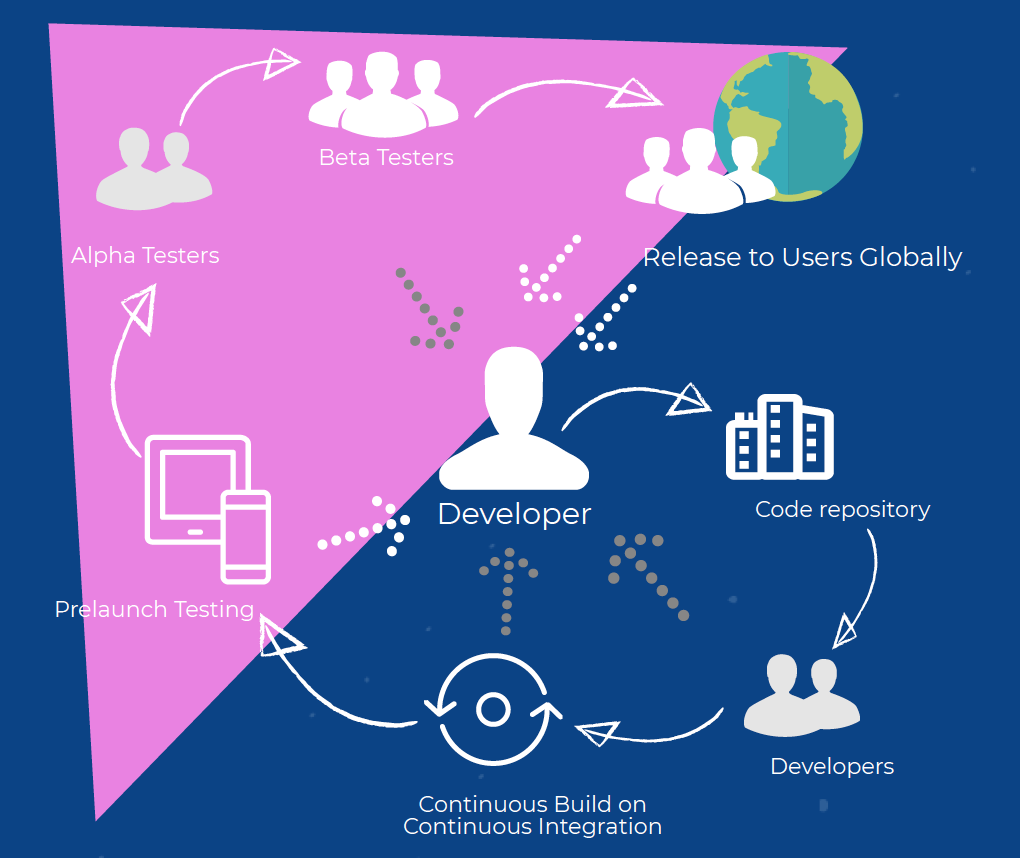
\includegraphics[width=13cm]{images/silvias-developer-centric-figure-mobilesoft2020.png}
    \caption{Sources of feedback for developers}
    \label{fig:sources-of-feedback-for-developers}
\end{figure}

Each source of feedback may stem from humans (for example, in reviews) or from software (for example, from code quality tools such as Lint). This research introduces three sources of software generated feedback.

\subsection{Research Strategy}
The research aims to provide practical and applicable insights to mobile apps developers. As such, the strategy was to predominantly work with development teams for mobile apps to ensure -- as far as practical -- the research is externally validated through their experiences, practices and feedback. As developers need to make choices appropriate to their context the research includes a variety of apps including commercial and not-for profit, small, medium and large development teams and user bases, and has an international flavour with developers situated in various continents including Asia, Europe, and the USA.

As the analytics tools also influence the results the research includes discussions and collaborations with several organisations who create these tools.


\section{My research methodology, and my choices}
As my main research question considers the application of analytics, the research needs to include a combination of usage \& analytics data where the analytics data is then applied with the intent of improving the product quality. The developers may not be successful in achieving improvements, although we hope they will be. They may also be able to improve their practices, so again their current and revised processes are also of interest.

Although I had prior experience in industry of the efficacy and potency of applying usage analytics to improve software development and testing of mobile apps, that experience is generally covered by confidentially agreements, and also the analytics tools have changed and developed markedly since those experiences. Therefore, action research seemed appropriate, particularly as one of the long-term opensource projects had extremely high failure rates according to the de-facto Android analytics tool. I decided it was appropriate and necessary to see if I could directly help that project to improve their mobile apps - \emph{``physician heal thyself"}\footnote{\href{https://en.wikipedia.org/wiki/Physician,\_heal\_thyself}{wikipedia.org/wiki/Physician,\_heal\_thyself}.}.

The next level of validity was that even if this work achieved the desired results, could other development teams achieve similar results by applying a similar approach? To help gain evidence the research engaged a separate opensource development project and development team. 

Working with non-profit opensource projects, where the teams are generally willing to make their practices and results public helps with being able to obtain information and publish the results. However, as many research projects discover, what might work for opensource projects - while important and interesting to the research community - might not matter much to the industry of professional and commercial development teams. 

Opensource apps are a tiny proportion of mobile apps available to users, so another level of learning and validation could be achieved through the insights of these professional and commercial development teams. Surveys tend to have poor response rates and lack the depth or richness I was seeking therefore I chose to engage at a deeper level as a fellow developer interviewing developers of several apps. Of course we would need the permission of their organisations, and some shared examples of their tools, their practices and their results of applying analytics well, and even times when they hadn't.

This research is not immune from also being improved, and similarly the process is likely to have plenty of scope for improvement as we learn more from the various projects, teams, apps, and analytics tools. Similarly, there is scope to find flaws, limitations, and weaknesses in the analytics tools, therefore there was scope in the research to share findings with the teams responsible for these, and related, software tools and to use the experiences and insights from any such sharing as part of this research.

Where practical, triangulation of data and analytics reports was used to help increase the confidence in the analytics and in the efficacy of using mobile analytics. As~\citep{marr2015bigdatabook} recommends:~\emph{``Measure metrics and data backed up or triangulated with other data sources."} and~\emph{``Where possible use a combination of data sets and triangulate the data. In other words, see if each data set delivers the same result so you can confirm and validate the answers."}. Triangulation of research methods is extensively covered in research. For example, \citep{fielding2012_triangulation_and_mixed_methods_designs} provides a rich discussion of triangulation and mixed methods design for various research areas. To the best of my knowledge  %SHOULD-DO decide how much to focus on triangulation, whether to discuss data triangulation as a technique for comparing analytics results (which doesn't seem to quite apply - at least in what I've read).



\begin{comment}
    - Could I try phrasing my RQs as OKRs to see if doing so helps me to improve the clarity and relevance of the RQs.
    - Also, how about creating annotated editions of my RQs where the annotations include context, commentary, connections to other RQs, notes on twitter-style answers to each, etc.
    - We want to know more about 'this' topic. Then provide Operational questions - to be addressed by the research, which will help us learn more about the topic.
    - What's a RQ and what's an analytical lens (to be used to help with the RQ)?
\end{comment}

\section{Research Questions}
\label{section-research-questions}

My research hypothesis is that using mobile analytics can help improve both the work development teams do and the quality of the product they create. Here work includes the development, bug investigation, and testing of the software being created. For the quality of the product I'm focusing on a subset of qualities, which are technology-centric.

The domain of mobile apps was selected for the research as mobile apps are ubiquitous, extremely popular, and have interesting and challenging contexts of use. And within the range of mobile apps the research ended up focusing on Android apps for various reasons including: the analytics tools available, the relative glut of suitable apps available for research, my prior experience and expertise, and their market share.

The core question the research aims to consider is: 
\emph{How can applying analytics improve software development and software testing for mobile apps?}~\label{overall-research-question}
Here the assumption is that analytics can help, as stated by Buse and Zimmermann ~(\citeyear{buse_analytics_2010}); and \emph{``with explicit and implicit feedback now available (almost) continuously, questions arise. How can practitioners use this information and integrate it into their development processes [to decide when to release updates]?"}~\citep{maalej2016_towards_data_driven_requirements_engineering}.

This leads to several related questions that underpin this main question \emph{i.e.}, These are grouped in three categories: sources, value, and impact.

\akb{There are a lot of sub-questions below. You will need to focus on the ones you have data to evaluate, or have more abstract formulations that cover groups of sub-questions.}

\yijun{If possible, you may need to dig out a few MobileSoft research papers to give evidence that these research questions have not been addressed in literature, e.g., \emph{Future Trends in Software Engineering Research for Mobile Apps}~\citep{nagappan2016_future_trends_in_sw_eng_for_mobile_apps}, whether the future work of some paper suggests one does not know the sources, value, or impact of mobile analytics to assess and improve app quality? Is there nothing in the general SE literature studying the "analytics" to "general software quality" problem? If there are such general work, how does "mobile analytics" and "app quality" differentiate the RQs to existing ones...}



\subsection{Sources}~\label{section-sources}
\begin{itemize}
    \item \emph{What sources of analytics are available?} at a superficial level there seem to be those that operate within the app and those that are external to the app, particularly those that gather data at the platform level. Several widespread analytics offerings were evaluated and several more were considered as part of this research and to provide an understanding of the overall context.
    \item \emph{How do the sources that were investigated compare in terms of the data they collect and how they are used?}
\end{itemize}

\subsection{Value}~\label{section-value}
Does using analytics provide quantitative and/or qualitative value that can be measured? Could it provide value in terms of assessing the quality of our work that was invested into developing, testing and preparing software before it was launched?
\begin{itemize}
    \item \emph{How truthy are various analytics offerings?} We discovered numerous errors in various analytics offerings. These results may be of interest to the research community given the endemic nature of mobile analytics in real-world apps in the major app stores.
    \item \emph{How much does the fidelity matter of the analytics offerings?} Can the results be used productively even if they are flawed?
    \item \emph{How does using the various analytics compare with other sources or reflections of software quality?} Research already studies how various sources, such as ratings and reviews, can be used to identify flaws in software. Where and how do analytics fit into the larger context of these tools. \emph{Note: I've not actively compared the sources from a practical perspective, however the Catrobat case-study may be relevant}.
    \item \emph{How can the analytics be used to inform and assess the work that went into creating and testing a particular release?} data from usage analytics can reinforce aspects of what was discovered pre-release (c.f. how Google Android's pre-launch reports cross-identify crashes) it can also identify quality flaws we missed in the development work.
    \item \emph{How can analytics help with bug investigation?} a single bug instance may be hard to assess in terms of the likely scope and impact on a user-base; how, where and when can analytics help with bug investigation? We might also consider practical limits e.g. that are enforced by the real-world analytics we used. 
\end{itemize}

\subsection{Impact}~\label{section-impact}
Here the focus is on whether the value has sufficient impact for anyone else to be interested in using and applying analytics. Given the nature of the research the main measures are practical, \emph{i.e.} in the real-world.
\begin{itemize}
    \item \emph{Do development teams use analytics in their practice?} If development teams find practices useful they will generally try to use them intrinsically. Do they? And if so, how?
    \item It's one thing to be able to improve a measurement such as the crash rate, it's also worth considering whether that has any material impact on other relevant measurements. \emph{Can we discern changes, even improvements, in user satisfaction, retention, etc. through using analytics?} One of the presumptions (identified in research) is that improving quality improves the user's satisfaction with mobile apps. If so, presumably we should be able to measure the effects, even crudely.
    \item \emph{Has anyone else found the work of interest? are there additional evidence of the impact of the work?} Here the main considerations are feedback from other researchers and from Industry e.g. Google.
\end{itemize}



\subsection{On Findings}
\yijun{It will be good to move 1.5 Research Questions here and articulate them as hypothesis or early hypothesis? It is too early to reveal the findings here Maybe you can prepare the reviewers by presenting the findings as confirmation of some "hypothesis", and first discuss about these hypothesis before introducing the facts? }

The research  the hypothesis 



\section{Outline of this thesis}


%%%%%%%%%%%%%%%%%%%%%%%%%%%%%%%%%%
\par\noindent\rule{\textwidth}{0.4pt}
%%%%%%%%%%%%%%%%%%%%%%%%%%%%%%%%%%
\section{The following need relocating}
Bugs are ubiquitous in software (even one of the most respected software engineers, Donald E. Knuth, recognises, publicly acknowledges, \emph{and pays for}~\cite{knuth_trutex, wikipedia__knuth_reward_checks_2020} bugs found in his creations. And self-aware developers expect there will be bugs in their software. \emph{``You are entitled to a reward of at least 0x$1.00 ($2.56) if you are the first person to report a bona-fide error not on those lists."} Donald E. Knuth~\cite{knuth_the_bank_of_san_serriffe}

Even top development teams are likely to learn of bugs they were not able to find, and cannot reproduce. For instance, Google's Android Auto Team have asked for help from end users to identify patterns that may help the team find and address a long-running and frustrating bug in Android Auto~\footnote{\url{https://support.google.com/androidauto/thread/2865341?msgid=44437416}}. As reported by \texttt{autoevolution} in May 2020:  
\emph{"As it turns out, the Android Auto team wasn’t able to reproduce the whole thing, so it’s now asking users to send additional reports with more information to help fix the problem."}~\footnote{~\url{https://www.autoevolution.com/news/google-wants-users-to-help-fix-widespread-android-auto-bug-143760.html}}.


\chapter{Related Work}
\label{chapter-related-work}
\begin{figure}
    \centering
    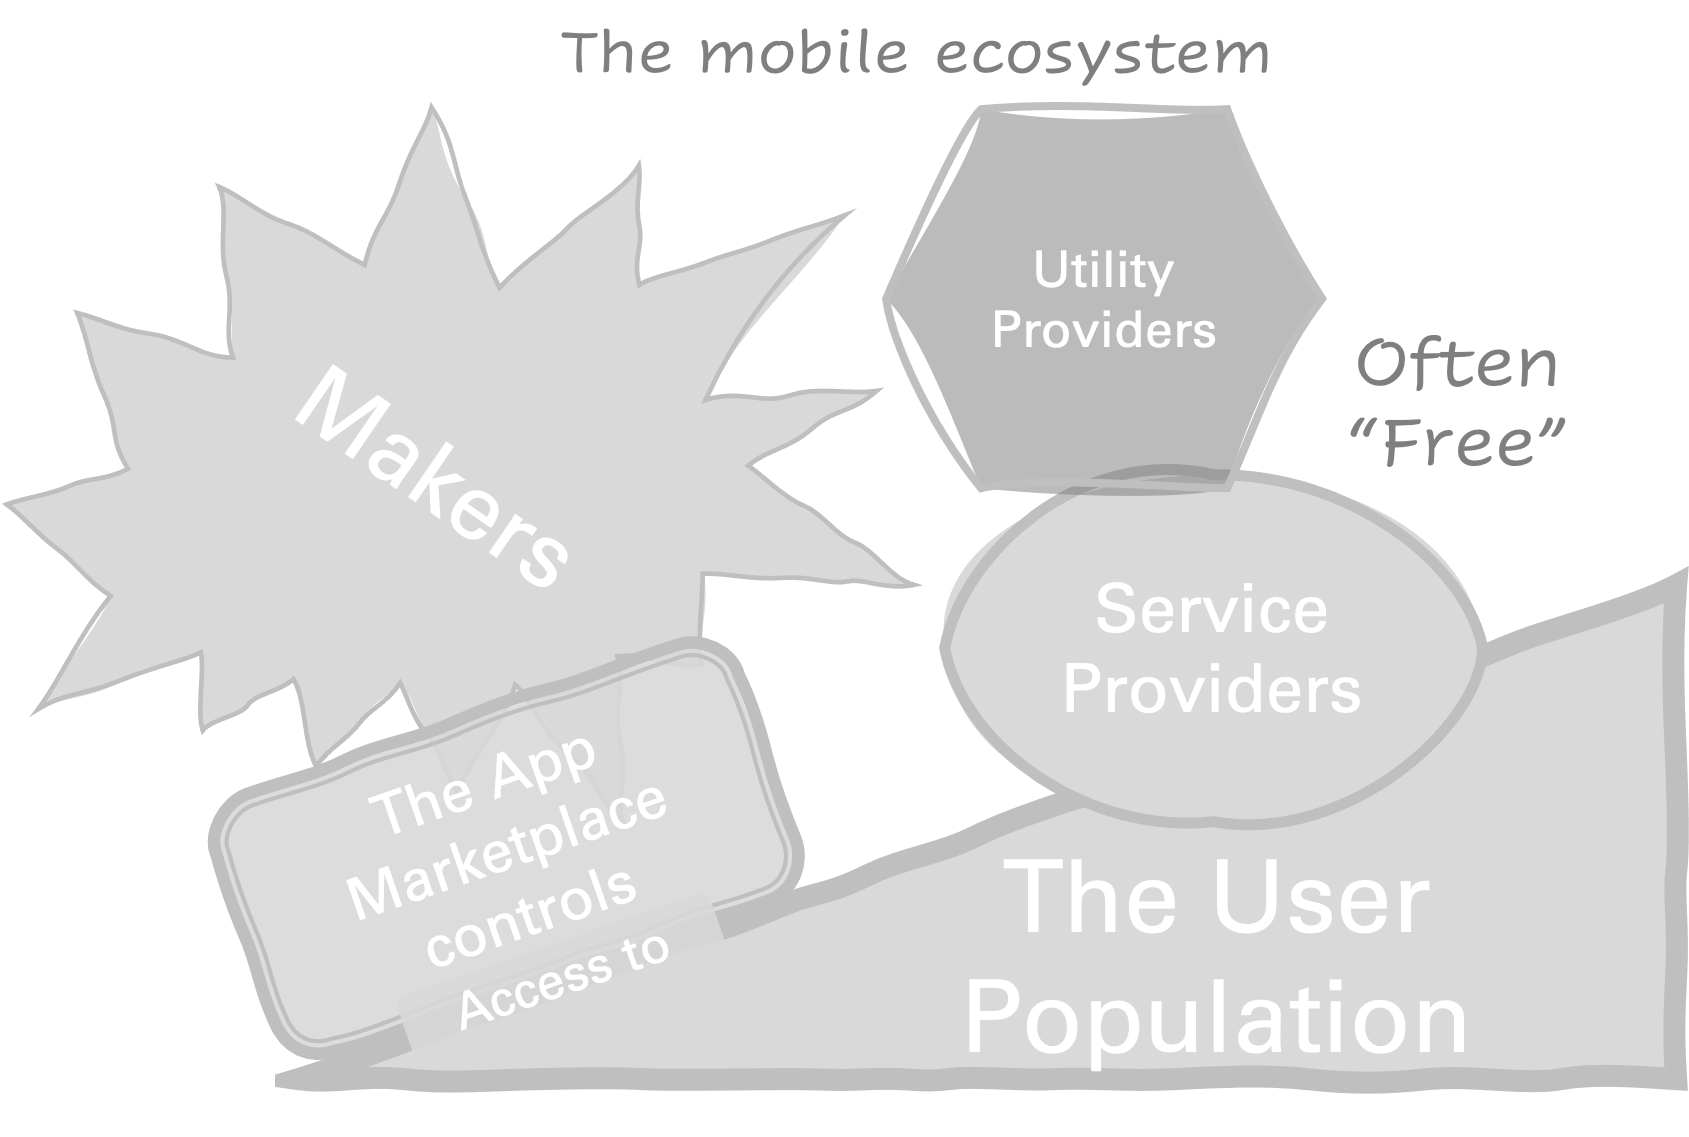
\includegraphics[width=0.8\textwidth]{images/my/the_mobile_ecosystem_sketch.png}
    \caption{The Modern Mobile App Ecosystem}
    \label{fig:my_modern-mobile-app-ecosystem}
\end{figure}

The modern mobile ecosystem, illustrated in Figure~\ref{fig:my_modern-mobile-app-ecosystem} sets the context for the thesis and this chapter together with the research questions. 
My work nestles within the works of many people in various related fields: in software quality, in analytics, and in the mobile device ecosystem. As researchers we understand and recognise there are gaps in the current state of the art, this chapter aims to identify several pertinent gaps which led to this research being performed, \emph{i.e.} which motivated me to act. The mobile ecosystems touch on billions of people's lives, where flaws in the apps and the ecosystem can adversely affect the lives of many of those people. 

Research in how mobile apps are created and tested, the relevance of app stores, service and utility providers, the user bases for mobile apps within the overall population of users of an app store ecosystem are all relevant. And meanwhile understanding why it's hard to create reliable software is also vital as part of acknowledging some of the grim realities development teams need to face if they are to succeed in their other goals and objectives for their mobile apps. An understanding of research into how to measure software qualities, and stability in particular, is key to establishing ways mobile analytics measures these qualities. At times this chapter will draw from broader sources, for instance in software development, testing, and analytics as these provide context for the particulars of the mobile app ecosystem. Conversely, in my view, and based on discussions at a peer workshop in Japan~\citep{nii_shonan_workshop_152}, I proposed a model, shown in Figure~\ref{fig:my_shonan_hysteresis_sketch}, that seemed to be well accepted and became part of the formal post-workshop report~\citep{nii_shonan_152_workshop_report}, where the mobile ecosystem is influencing the desktop app ecosystems. Examples include: app stores, per user licensing across multiple devices, public ratings and reviews, platform (device) level, crash reporting, and usage analytics, and so on.

\begin{figure}
    \centering
    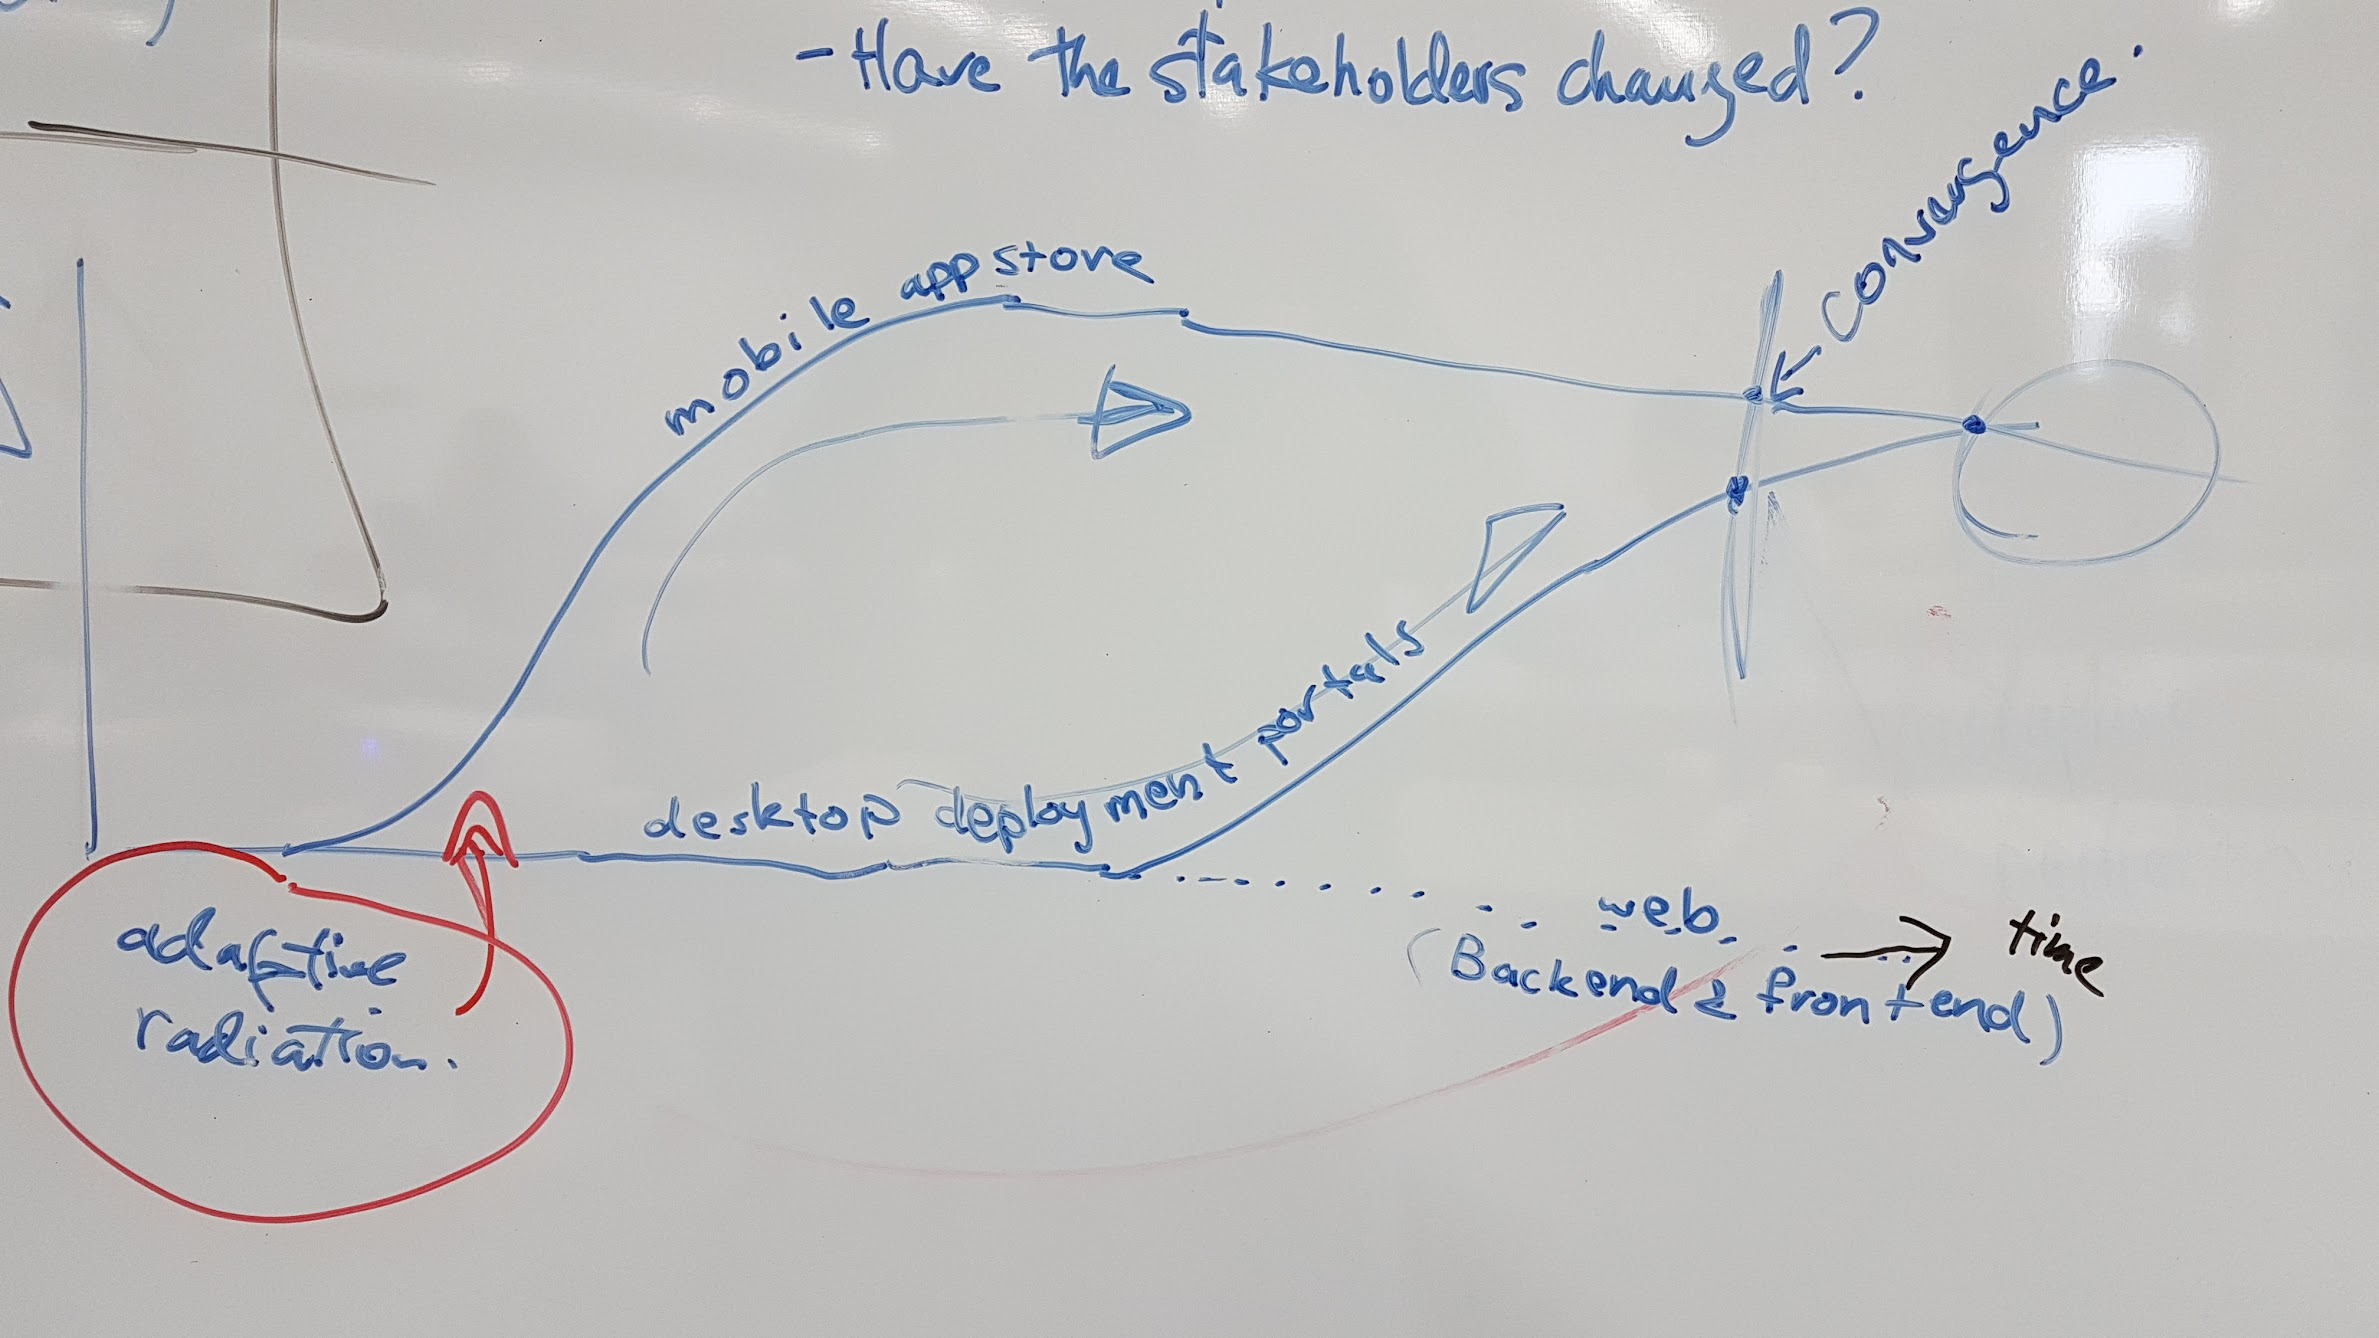
\includegraphics[width=0.8\textwidth]{images/nii-shonan-workshop-152/shonan_hysteresis_diagram_20191210_132528.jpg}
    \caption{Mobile and Desktop Growth and Convergence}
    \label{fig:my_shonan_hysteresis_sketch}
\end{figure}
.


The practicalities of the research and the case studies where nearly all the work pertains to the Google Android ecosystem also helps in the selection criteria of relevant related works. As the vast majority of active research in the domain of mobile apps also pertains to this ecosystem means the topic is richly served in terms of related works.

\section{The mobile app ecosystem}

Dated works when BlackBerry and Windows Phone app stores existed. Mainly to set the context and identify there has been plenty of research into generations of the ecosystem.


\section{Making mobile apps}
Mobile apps need to be made and developers make them. There are various working practices, apps are made by visionaries, employees, amateurs, and communities. Many claim to be ``Agile" in their working practices. There are various activities involved including development, testing, release, and deployment. Figure~\ref{fig:my_mobile-app-makers} highlights these activities as part of the overall ecosystem.

\begin{figure}
    \centering
    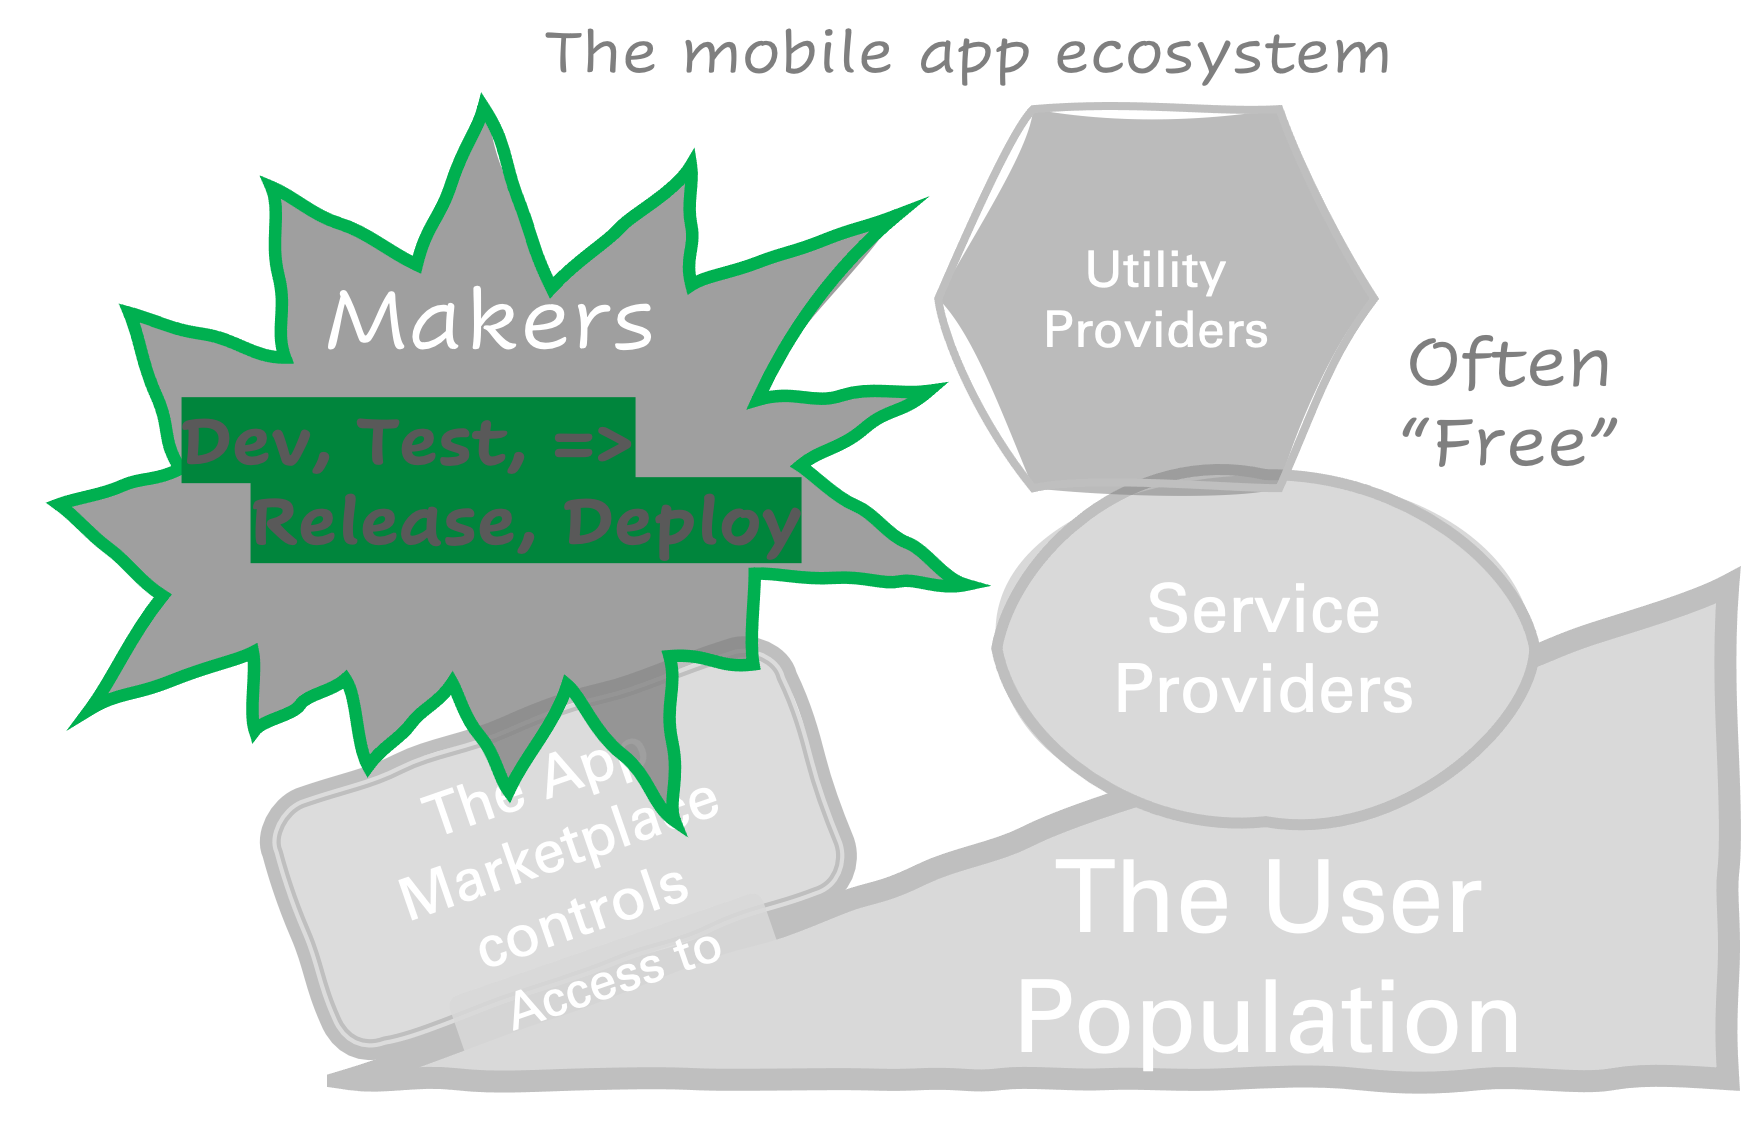
\includegraphics[width=0.4\textwidth]{images/my/the-mobile-app-ecosystem-makers-dtrd.png}
    \caption{Makers of mobile apps}
    \label{fig:my_mobile-app-makers}
\end{figure}

Unending materials are written and published online on making apps, beautiful apps, elegantly engineered apps, those that use and apply various software libraries (which we will cover in the providers section). There are a plethora of books and research materials available too. 

Books:

\subsection{Papers}

\textbf{Development practices}

Advertising in apps: 

\textbf{Testing practices}

\textbf{Code Quality: Static Analysis}

\textbf{Release and Deployment practices}

When to release an app:

%%%%%%%%%%%%%%%%%%%%%%%%%%% End of the fresh version of this chapter %%%%%%%%%%%%%%%%%%%%%%%%%%%%%%%%%%%%%%%%
\clearpage
%%%%%%%%%%%%%%%%%%%%%%%%%%% Earlier material follows %%%%%%%%%%%%%%%%%%%%%%%%%%%%%%%%%%%%%%%%%%%%%%%%%%%%%%%

Android, given its mainly opensource codebase and popularity as a platform (Number 1 globally) is also well researched with 53 papers on the topic at ICSE 2020 and related conferences and workshops \href{https://conferences.computer.org/icse/#!/search}{ICSE 2020 Search Page}, whereas only 3 papers were on the also extremely popular iOS platform at the same set of conferences and workshops.

\begin{figure}[htbp!]
    \centering
    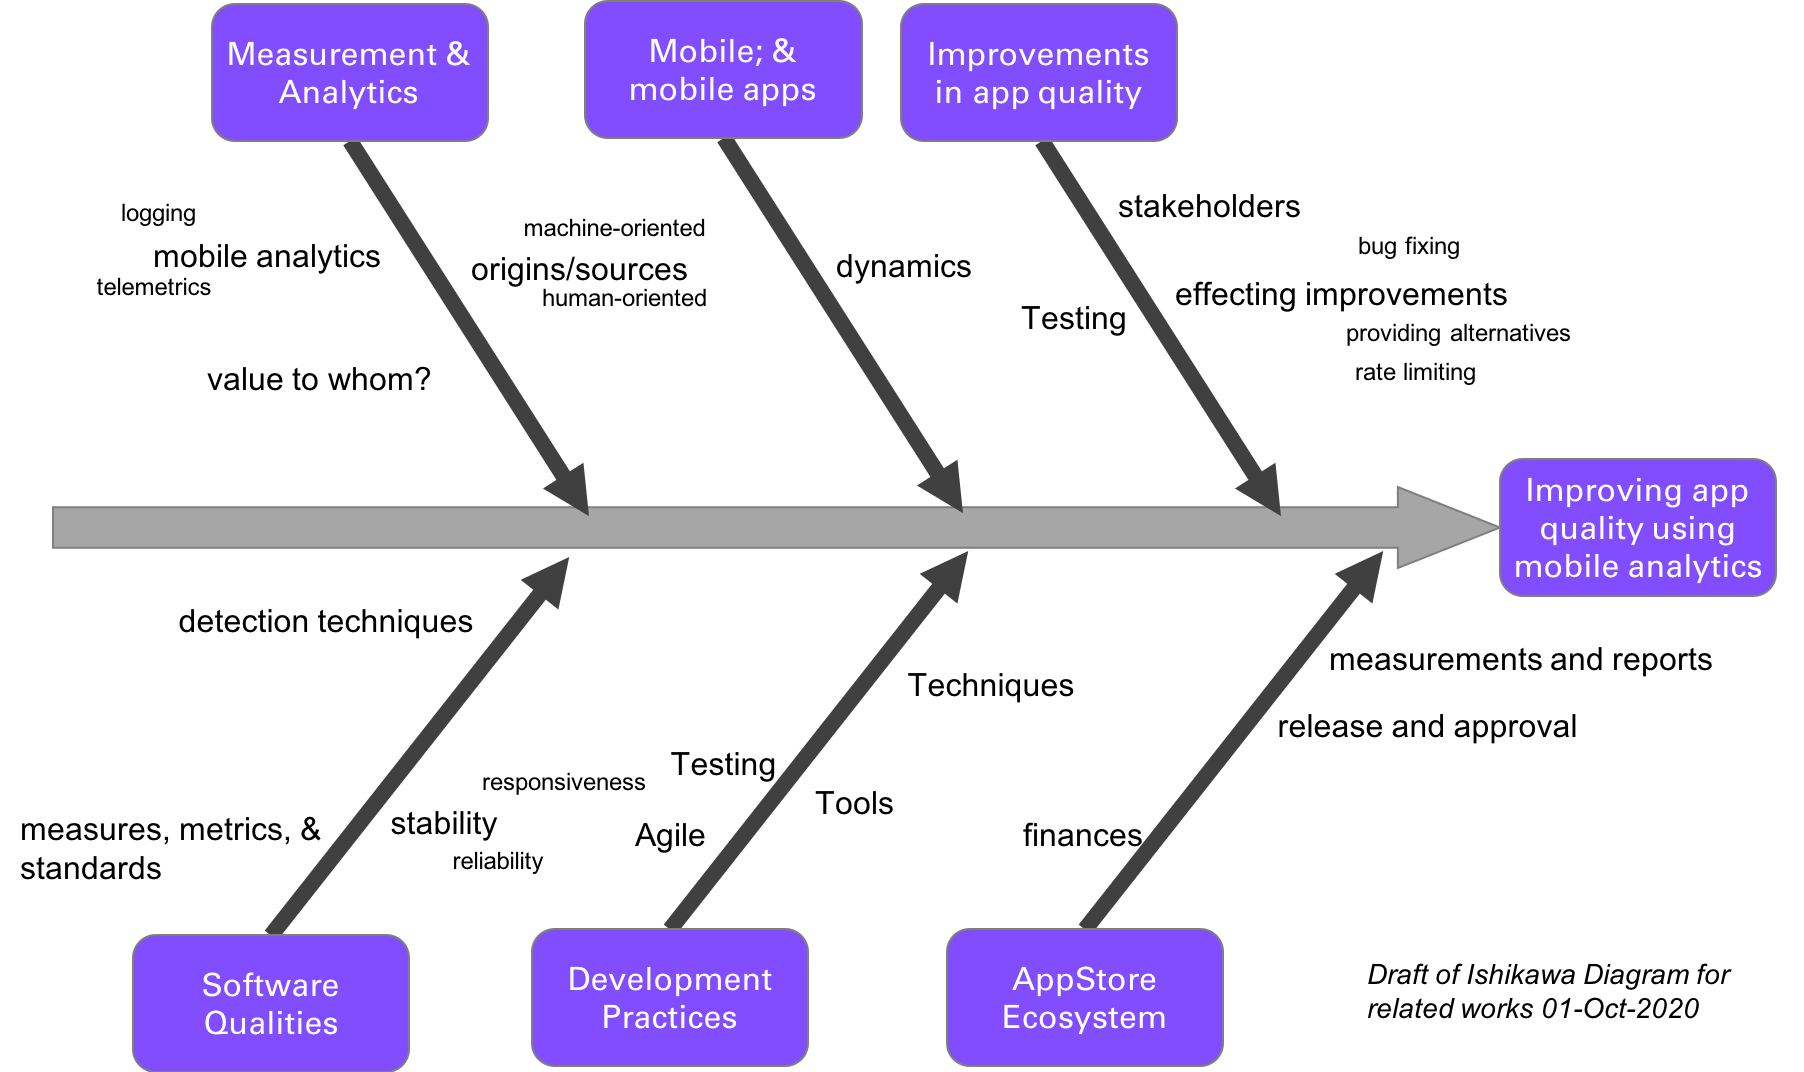
\includegraphics[width=15cm]{images/related-works-ishikawa-diagram-01-oct-2020.png}
    \caption{Ishikawa diagram for topics related to this thesis, }
    \label{fig:related_works_ishikawa_diagram}
\end{figure}

Ishikawa diagrams, also known as fishbone diagrams, can help illustrate the relationships and relevance of various topics to the overall objective. Figure~\ref{fig:related_works_ishikawa_diagram} is an example of an Ishikawa diagram for Service Support, with the aim of providing [good] quality air travel service~\cite{itil_ishikawa_example}. 
\akb{No need to provide a separate example of an Ishikawa diagram - you can explain the diagram features / notation using the diagram you've produced for your research. }
%%%%%%%%%%%%
% Learn more about Ishikawa diagrams
% https://www.moresteam.com/toolbox/fishbone-diagram.cfm 

\section{Topics to include in this chapter}
The following hierarchical list includes topics I plan to include in this chapter, after this section.


\begin{itemize}
    \item An overview on~\href{software.quality}{\emph{software quality}} including various viewpoints of quality e.g. Gerry Weinberg):
    \begin{itemize} 
        \item ISO standards
        \item Software defects, faults and failures~\hyperlink{defects.faults.failures}{\emph{link}}
        \item Bug investigation and localisation
        \item QoE: Quality of Experience
        \item Classic references e.g. Phadke~\citep{phadke1995_quality_engineering_using_robust_design} and perhaps Non-functional requirements in Software Engineering? 
        \item relevant / related academic research in my field
        \item Reliability. Introduced in ~\hyperlink{software.quality}{Software Quality}, and then expanded in a subsection~\hyperlink{software.reliability}{\emph{here}}
        \item Then focus on stability (as used by HP and then Google) encompassing reliability, freezes, etc.
        \item Discuss MTBF, usage paths and profiles and their effects on the measured values
        \item Maslow's hierarchy of needs where reliability is one of the base levels, yet vital. c.f Sommerville.
    \end{itemize}
    \item Measurement and Analytics
    \begin{itemize}
        \item Views from outside software engineering e.g. how to measure anything book
        \item Logging
        \item Telemetry
        \item Software Analytics e.g. Buse and Zimmermann
        \item Software Analytics tools and concepts e.g. free the data.
        \item Sources and mechanisms for collecting data and information about mobile apps
        \begin{itemize}
            \item Human-centric sources e.g. ratings and reviews. Perhaps also discuss some of the flaws and limitations either here or in the 'caveats...' section later?
            \item Perhaps also consider in-app feedback c.f. the Mobile Twin Peaks paper?
            \item Alpha, Beta, Crowd, and other forms of testing with subsets of a population.
            \item Program-centric sources e.g. logging, crash reporting libraries, analytics libraries, platform-level observations.
        \end{itemize}
        \item Using Data
        \item Privacy and Control
    \end{itemize}
    \item Software Development Practices
    \begin{itemize}
        \item Agile development and the effects on the software that is developed and released.
        \item Motivations for/of software developers.
    \end{itemize}
    \item Software Testing
    \begin{itemize}
        \item Schools of Software Testing? Old work that might help set the scene
        \item Classic references on software testing e.g. Boris Beizer
        \item using testing to measure quality and measuring software testing e.g. effectiveness.
    \end{itemize}
    \item App Stores and their effects on software development and engineering
    \begin{itemize}
        \item App Stores as ecosystems
        \item Release Planning (c.f DevOps and Release Engineering (including Shonan)
        \item Ratings and Reviews
        \item Google Play (and other Android app stores)
    \end{itemize}
    \item Developing mobile apps
    \begin{itemize}
        \item Single and multi-platform approaches
        \item A brief history of mobile app development
        \item Various species of bugs that affect mobile apps
    \end{itemize}
    \item Testing of Mobile Apps (this might be a distinct section in the Related Works as it's a rich topic). Do we care about testing of mobile apps that predates app store ecosystems?
    \begin{itemize}
        \item Automated testing frameworks and tools
        \item Testing practices (from both research and practical perspectives)
        \item Test Oracles
        \item Device Selection (as one aspect of testing for bug identification and investigation)
        \item Testing by crowds
        \item Measuring the efficacy of testing
    \end{itemize}
    \item Mobile Analytics~\hyperlink{mobile.analytics}{\emph{link}}
    \begin{itemize}
        \item types and sources of mobile analytics (also refer to appendix)
        \item Using Mobile Analytics to assess app behaviours
    \end{itemize}
    \item Caveats, constraints, flaws, limitations
    \begin{itemize}
        \item For instance on blind-spots, excessive trust and the ironies of automation. 
        \item Using crashes, ANRs, etc. as the test oracle - what will we miss if we only consider these aspects? how relevant is what we miss and what can we do to fill in some of the gaps?
    \end{itemize}
    \item Has anyone else published in my areas of research?
\end{itemize}

\hypertarget{software.quality}{}
\section{Software Quality}
Software quality is multi-faceted, and as the article by~\citep{kitchenham1996_software_quality_elusive_target} states, an \emph{elusive target}. This article builds on five different perspectives of quality Some facets are more user-centric, such as perceived quality by end-users, which may include aesthetics, responsiveness, brand perception, other facets focus on more technical aspects such as whether an app freezes, crashes, or whether an app corrupts, leaks, or loses data, for instance. 


I cannot hope to %or it would be impractical and potentially counter-productive to
cover all the facets even after many years of working and researching in this domain. Instead I have selected the facets germane to my PhD research.

%Expand on software quality generally before leaping into specifics.
In the 1980's and 1990's software quality became an important and established topic, with several seminal publications including:~\citep{garvin1984_what_does_product_quality_really_mean},~\citep{weinberg1992quality}, and~\citep{kitchenham1996_software_quality_elusive_target}. If we start with Weinberg who stated \emph{"Quality is value to some person"}~\cite{weinberg1992quality}. To paraphrase him, \emph{Quality is in the eye of the beholder}. For mobile apps the majority of the beholders are the end users, however the app store could also be considered a beholder, and certainly they have the power to be prosecution, judge and jury when determining which apps are allowed to be live in the app store, and which ones to promote, and which end up lower in the search results.

Considering the other two papers mentioned earlier, Garvin introduced five approaches to defining quality: 1) transcendent, product-based, user-based, manufacturing-based, and value-based. His work was extended by Kitchenham and Shari Lawrence Pfleeger. One of their key wry observations was that standards, such as ISO 9001 and ISO 9126, and maturity models, such as the Capability Maturity Model, focus on a consistent process rather than a quality product, and that~\emph{``there is little evidence that conformance to process standards guarantees good products."}~\citep{kitchenham1996_software_quality_elusive_target}. To the best of my knowledge, neither ISO standards nor maturity models figure highly for the vast majority of mobile app development teams, therefore I have considered and then chosen not to use the formal software quality models or standards in my research. 

In their discussion of the value-based view there are several foundations that were highly relevant at the time, where users were involved in product specifications and~\emph{``equating quality to what the customer is will to pay [for]"}. For mobile apps, the users are seldom involved in the specification and they do not pay with money for the vast majority of the apps they use, instead they may pay with their data... So a possible refinement of value-based views for mobile apps is to consider quality to what customers are willing to~\emph{use}? i.e. if they continue to use the app then the quality could be deemed to be adequate.

In terms of measuring quality, the authors observed,~\emph{``When users think of software quality, they often think of reliability"}~\citep{kitchenham1996_software_quality_elusive_target}. They later extend this claim and say~\emph{``[users] are also concerned about usability, including ease of installation, learning, and use."}
%
For mobile apps, these five approaches are relevant to varying degrees: development teams often internalise Agile concepts into their thinking and their practices, %MUST-DO continue this thought process here.

I will cover the both the product and manufacturing views of quality later in this thesis, particularly in several of the case studies.

% NB there is a lot more relevant and interesting material in the Kitchenham paper - see the handwritten notes on the printed copy for examples.

% \akb{You will need to choose an existing taxonomy of software quality and explain which aspects are relevant to your research before discussing literature from each of these aspects. The Kitchener et al paper below is a good starting point for this.}

In "Software Quality: The elusive target"~\cite{kitchenham1996_software_quality_elusive_target}. their work also presents two further points: The context is important when we aim to assess ``adequate" quality in a software product. And \emph{"A good definition [of software quality] must let us measure quality in a meaningful way. Measurements let us know if our techniques really improve the software, as well as how process quality affects product quality."}

%SHOULD-DO cover Quality of Experience (QoE) here. How users perceive QoE, how users communicate their QoE in an app store ecosystem, etc.

% Placed here with other material on reliability. MUST-DO Decide whether it's still needed and either integrate or remove.
Reliability is a key facet of software quality and a measure of how reliable (error-free) software is in use. Poor reliability risks jeopardising mobile apps as few users want to use an unreliable app. 
%\yijun{Why do you focus on reliability as the only facet of quality after dismissing the other facets? Do you need to worry about correctness as another quality facet related to testing?} 

As mentioned in the introduction, reliability is considered a key attribute of software quality~\citep{febrero2017_software_reliability_as_user_perception}. In their research they focus on trying to improve the understanding of an software reliability in industry. 

Maslow's hierarchy of needs~\citep{wikipedia_maslows_hierarchy_of_needs} provides a five-layered conceptual model of human needs, where lower levels dominate higher levels until they are at least partially satisfied. Reliability of software may similarly be one of the lower levels of a hierarchy of software quality, where inadequate reliability dominates until it is adequately satisfied. In some ways adequate reliability may be a hygiene factor for mobile apps and their developers. Once reliability is more than adequate developers can choose to focus more on higher level quality needs such as aesthetics as part of improving usability, and so on.

The performance and reliability quality aspects of software have been key topics for decades, including the work of Raj Jain in his seminal book~\emph{`The art of computer systems performance analysis'}~\cite{jain1991art}, a work that influenced me at the time as well as many others. One example of that influence was research into various software qualities that I and others collaborated in for over a decade, and taught and presented internationally. This included the concept of non-functional requirements and non-functional testing. Three related measures were identified related to requests for service of a computer system: performance if the request was successful, reliability if the request received an error, and availability if the request could not be performed. This is illustrated in Figure~\ref{fig:three-possible-ourcomes}~\footnote{Figure used with permission, and presented in a keynote at the StarEast 2005 conference author~\cite{harty_stareast2005_keynote}}. 

Poor reliability damages the trustworthiness and credibility of software, Ian Sommerville notes:~\emph{``... reliability was probably the most important product attribute as unreliable systems are discarded or never brought into use."}(p. 592, ~\cite{sommerville1989_software_engineering}). One of the key considerations for Sommerville is the operational reliability, and as he notes, in~\cite{mills1987_cleanroom_software_engineering}, removing software faults from seldom used code is unlikely to make a material improvement in the perceived reliability. Effective improvements need to focus on faults in frequently used code, and particularly where the failures are perceived by users of the software.

\begin{figure}[htbp!]
    \centering
    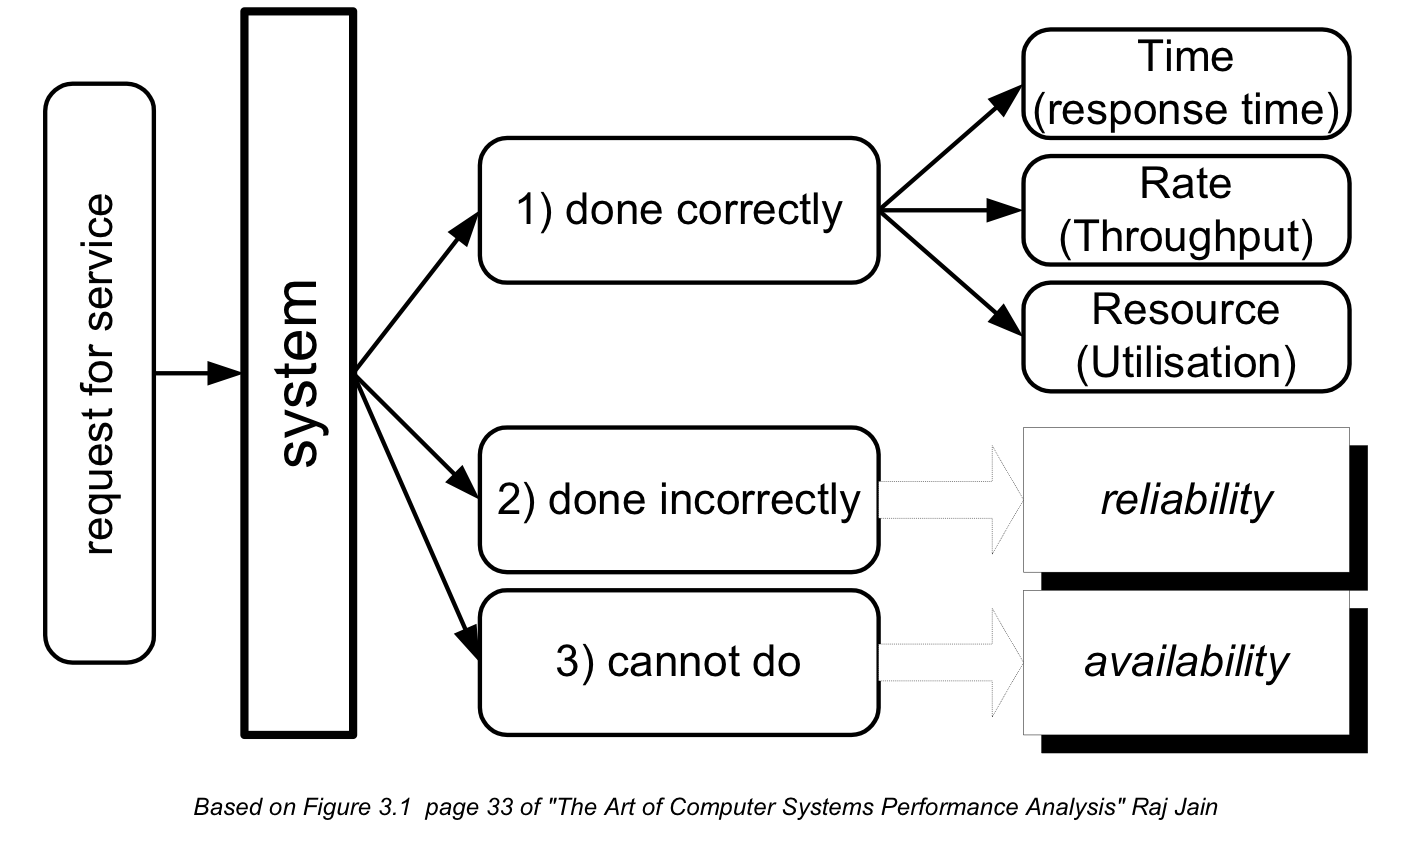
\includegraphics[width=14cm]{images/commercetest/raj-jain-performance-reliability-availability.png}
    \caption{Three possible outcomes}
    \label{fig:three-possible-ourcomes}
\end{figure}

The main software quality my research investigates is reliability as measured through counting and analysing crashes of mobile apps. While these might seem to be mundane compared to more attractive topics such as user experiences, poor reliability can undo the success of an otherwise attractive and performant software application. As Bavota~\emph{et al} observe in~\cite{bavota2014_impact_of_api_change_android} ~\emph{``users easily get frustrated by repeated failures, crashes, and other bugs; hence, they abandon some apps in favor of their competition."} Also app crashes are one of the the three most frequent complaints (together with functional errors and feature requests) found by (\cite{khalid2015_what_do_mobile_app_users_complain_about}) in their studies of 6,390 low-rated user reviews for 20 free to download iOS apps. And from a practical perspective Google states \emph{``Fixing issues can lead to a better user experience, higher ratings, and more retained installers."} in their pre-launch reports.

Crashes adversely affect reliability. They also increase the risk of users abandoning a mobile app~\citep{dimensionalresearch2015_mobile_app_use_and_abandonment}. Development teams need ways to manage risks, they also need ways to conceptualise and personalise risks according to~\citep{pfleeger2000_risky_business}. In a set of handouts paraphrases the description of risk management elegantly as \textit{``Plans to avoid these unwanted events or, if they are inevitable, minimize their negative consequences."}~\citep{amland2002_slides}~\footnote{Note: these slides are based on by a similar peer-reviewed paper of a case study that applied risk-based testing in a financial [non-mobile] application~\citep{Amland_2000_rbt_financial_case_study}.}


%\yijun{Logically I don't see the connection between quality facets => quality (general) => reliability (facet) again, perhaps you want to add some transitions so readers can follow the thoughts.}

Crash data is impersonal and oft requested and collected by operating systems and applications. For instance, when an Apple operating system is updated users are asked a couple of questions including whether they are willing to share crash data with Apple and with developers [of apps].

Unresponsive software~\emph{e.g.} when software freezes, is also problematic and may lead to poor user experiences and apps being abandoned and uninstalled. In contrast to crashes, unresponsive software may be harder to measure unequivocally. In Android Google established the term \emph{Application Not Responding (ANR)} and imbued it with distinct measurable criteria %TODO add these.



%%%%%%%%%%%%%%%%%%%%%%%%%%%%%%




\textbf{Bug investigation and localisation}: A failure, such as a crash, provides a data point. A challenge of interest to both research and industrial practice is to learn enough about the failure to be able to make an actionable decision. Bug investigation and fault localisation 
are critical activities where participants frequently have various constraints they need to work within including the time they have available, the return on investment of each stage of their work, and so on.

\begin{figure}
    \centering
    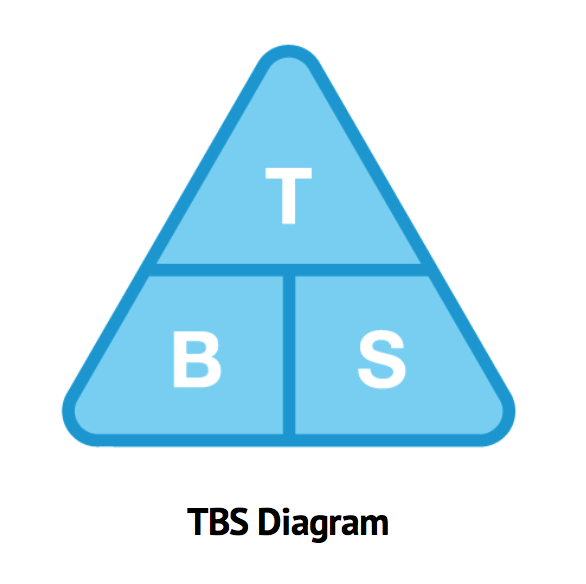
\includegraphics[width = 0.5\textwidth]{images/mobile-analytics-playbook/TBS.png}
    \caption{TBS diagram, originally in~\citep{harty_aymer_playbook_2016}}
    \label{fig:my_tbs_diagram}
\end{figure}

% c.f. T.B.S. Jon Bach
Bug investigation takes time and incurs various costs, with rare exceptions it is not done voluntarily. Repurposing and generalising Jon Bach's work on a concept he devised called ``TBS" metrics and reproduced below:

“TBS” metrics. Test design and execution means scanning the product and looking for problems. Bug investigation and reporting is what happens once the tester stumbles into behavior that looks like it might be a problem. Session setup is anything else testers do that makes the first two tasks possible, including tasks such as configuring equipment, locating materials, reading manuals, or writing a session report."~\citep{bach2000_sbtm}

Software Design and Development encapsulates the work developers of mobile apps \emph{intend} to do to create and improve mobile apps. Bug investigation and reproduction describes their focus when they are involved in understanding failure of their app. And session setup is anything else they need to do to make the first two tasks possible. Perhaps \emph{``DBS" metrics} would be a useful complement to ``TBS" metrics?

One of the arguments Jon Bach makes in various presentations is to maximise the T and minimise the B.S. This is illustrated in Figure~\ref{fig:my_tbs_diagram}.

% If practical include examples of Jon's squiggle diagrams, e.g. see slide 15 in  https://www.slideshare.net/TechWellPresentations/exploratory-testing-is-now-in-session

As many practitioners know, time spent investigating and addressing failures and related flaws in the code is time that is not available to work on features or other new stuff. As I discovered in one case study in particular, the development team may choose to only fix failures they perceive as easy to find and fix. One of the open challenges is to reduce the perceived and actual effort developers need to apply to address runtime failures in their mobile apps. 
%
Perhaps application of mobile analytics can improve bug investigation and bug localisation? 



MUST-DO continue by writing about \citep{avizienis2004_basic_concepts_and_taxonomy}.


Diagnosis:

Repair: where the effort is materially less than the benefits that result from the repair. 


One of the measures applied here is using \emph{relative correctness}, a concept introduced in~\cite{diallo2015_correctness_and_relative_correctness}, ~\emph{``the
property of a program to be more-correct than another with respect to a given specification"}. The authors believe using relative correctness as a concept leads to simpler programs enhanced  in steps. This approach, of stepwise correctness-enhancing transformations, may be useful and productive in terms of using mobile analytics to improve the quality of software, and in particular the mobile apps used in our case studies. 

Research into faults and faulty programs~\cite{mili2014_on_faults_and_faulty_programs}~\footnote{And also their presentation on the topic:~\href{http://mathcs.chapman.edu/ramics2014/slides/MiliFriasJaouaRAMiCS2014.pdf}{On faults and faulty programs}} is also relevant as mobile app developers may choose to \emph{``make the program less incorrect"}~\cite{mili2014_on_faults_and_faulty_programs}. The authors also make several pertinent statements, slightly reworded from their presentation slides here for clarity:
\begin{itemize}
    \item Hypothesis: ``If a program passes the test, it is correct (fault removal confirmed)." However, the program may work when tested but fail outside [in real use].
    \item Hypothesis: ``If a program fails the test, it is incorrect (fault removal should be rolled back)." However, the program does not have to be correct; only more-correct than original. Other tests may now pass that would not have passed for the unmodified version of the program.
\end{itemize}

Improving reliability, provided it does not adversely affect other desirable qualities of a program may be considered a pragmatic and sensible option for developers, especially when they cannot guarantee their software will be fault free and they need to respond quickly to the needs of the market and their end-users.



\subsection{Seven Quality Control Tools}
Ishigawa's work extended beyond the eponymous Ishigawa, or fishbone, diagram %(as illustrated in Figure~\ref{fig:ishikawa_example_itil})
; he also devised seven basic tools for quality, in turn inspired by W. Ewdards Deming's lectures in Japan in the 1950's~\cite{7_basic_quality_tools_with_R}.

Of these seven tools, two are of particular interest in my research, his diagram to help set this work in context, and Pareto charts (also known as the Pareto distribution diagram), illustrated in one of the appendices~\hyperlink{pareto.diagrams.in.r}{\emph{here}}.


\hypertarget{defects.faults.failures}{}
\subsection{Software Defects, Faults and Failures}
\emph{Add a preamble to why this subject is relevant to my research - set this topic in context. Keep the examiner on the red thread of my research.}
\yijun{The heading doesn't match yet with the content: what about Faults and Failures? You may consider this standard for one definition:
\url{https://ece.uwaterloo.ca/~agurfink/ece653/assets/pdf/W01P2-FaultErrorFailure.pdf}}


According to Mäntylä and Itkonen more defects were found implicitly (62\%) than explicitly (38\%) ~\cite{mantyla2014_how_are_software_defects_found}, based on a survey of four software development companies in three different companies. The authors state \emph{"Implicit defect detection has a large contribution to defect detection in practice, and can be viewed as
an extremely low-cost way of detecting defects."}. Similarly my research may be considered as a useful source of finding defects implicitly, where the defects are mined and reported by mobile analytics tools and development teams can decide on the defects they deem sufficiently relevant \emph{and} practical to fix. I will discuss separately some of the implications of applying this approach to complement other approaches.

\emph{Add the take aways of why I've included this topic. Be clear about why using analytics is different from what's been done before. Explain the gaps in prior work}

~\hypertarget{software.reliability}{}
\subsection{Software Reliability}
Over twenty years ago, in a paper published at ICSE in 1997, the authors (Frankl, Hamlet, and Littlewood) discussed approaches to select testing methods to deliver reliability. They identified two main goals in testing software: 
\begin{enumerate}
    \item to \emph{achieve} reliability~\cite{frankl1997choosing_testing_for_reliability} (using testing to probe software for bugs so they could be removed to improve the reliability), and 
    \item to \emph{evaluate} reliability, an approach they call \emph{operational testing}, where tests reproduce the expected usage of software and testers wait for failures to occur.
\end{enumerate}

Both approaches provide a mixed bag of desirable and undesirable effects; in the paper the authors compare the testing effectiveness based on the reliability of the program after it was tested. In their conclusion they state: \emph{"research cannot offer decision makers a best testing method for all situations."}. Instead they believe research can offer better criteria for informing the choice of a method to suit a decision maker's specific situation. They also hope to guard against, and help people avoid, illogical decisions.

Their work intersects with the work of Dorothy Graham's proposed measure of Defect Detection Percentage (\emph{DDP}, for short)~\cite{graham_measuring_2009} aimed at evaluating the effectiveness of whatever testing was performed by comparing the issues found during testing with those found subsequently, often when the software is in use by others.

Frankl, Hamlet, and Littlewood discussed operational testing based on expectations of the inputs; in turn a paper by Bishop in 1993~\cite{bishop1993variation} discussed the variation in software survival time depending on differences in the operational input profiles. Failure probabilities are not constant, the paper states the probability of failures decreases as the time from the last failure increases. There are several relevant observations in the paper, including: \emph{"During a failure, restarting the software will have little effect if the input conditions are similar..."} for instance a mobile app may crash repeatedly if a user (for instance) happens to repeat an action that exercises the code that fails. This was observed this behaviour in Kiwix, one of the Android apps under evaluation, where a single crash occurred 55 times for a single user, as Figure~\ref{fig:55-crashes-missing-webview-package-exception}.
%\yijun{It is good to confirm the points in your observation.}

\begin{figure}[htbp!]
    \centering
    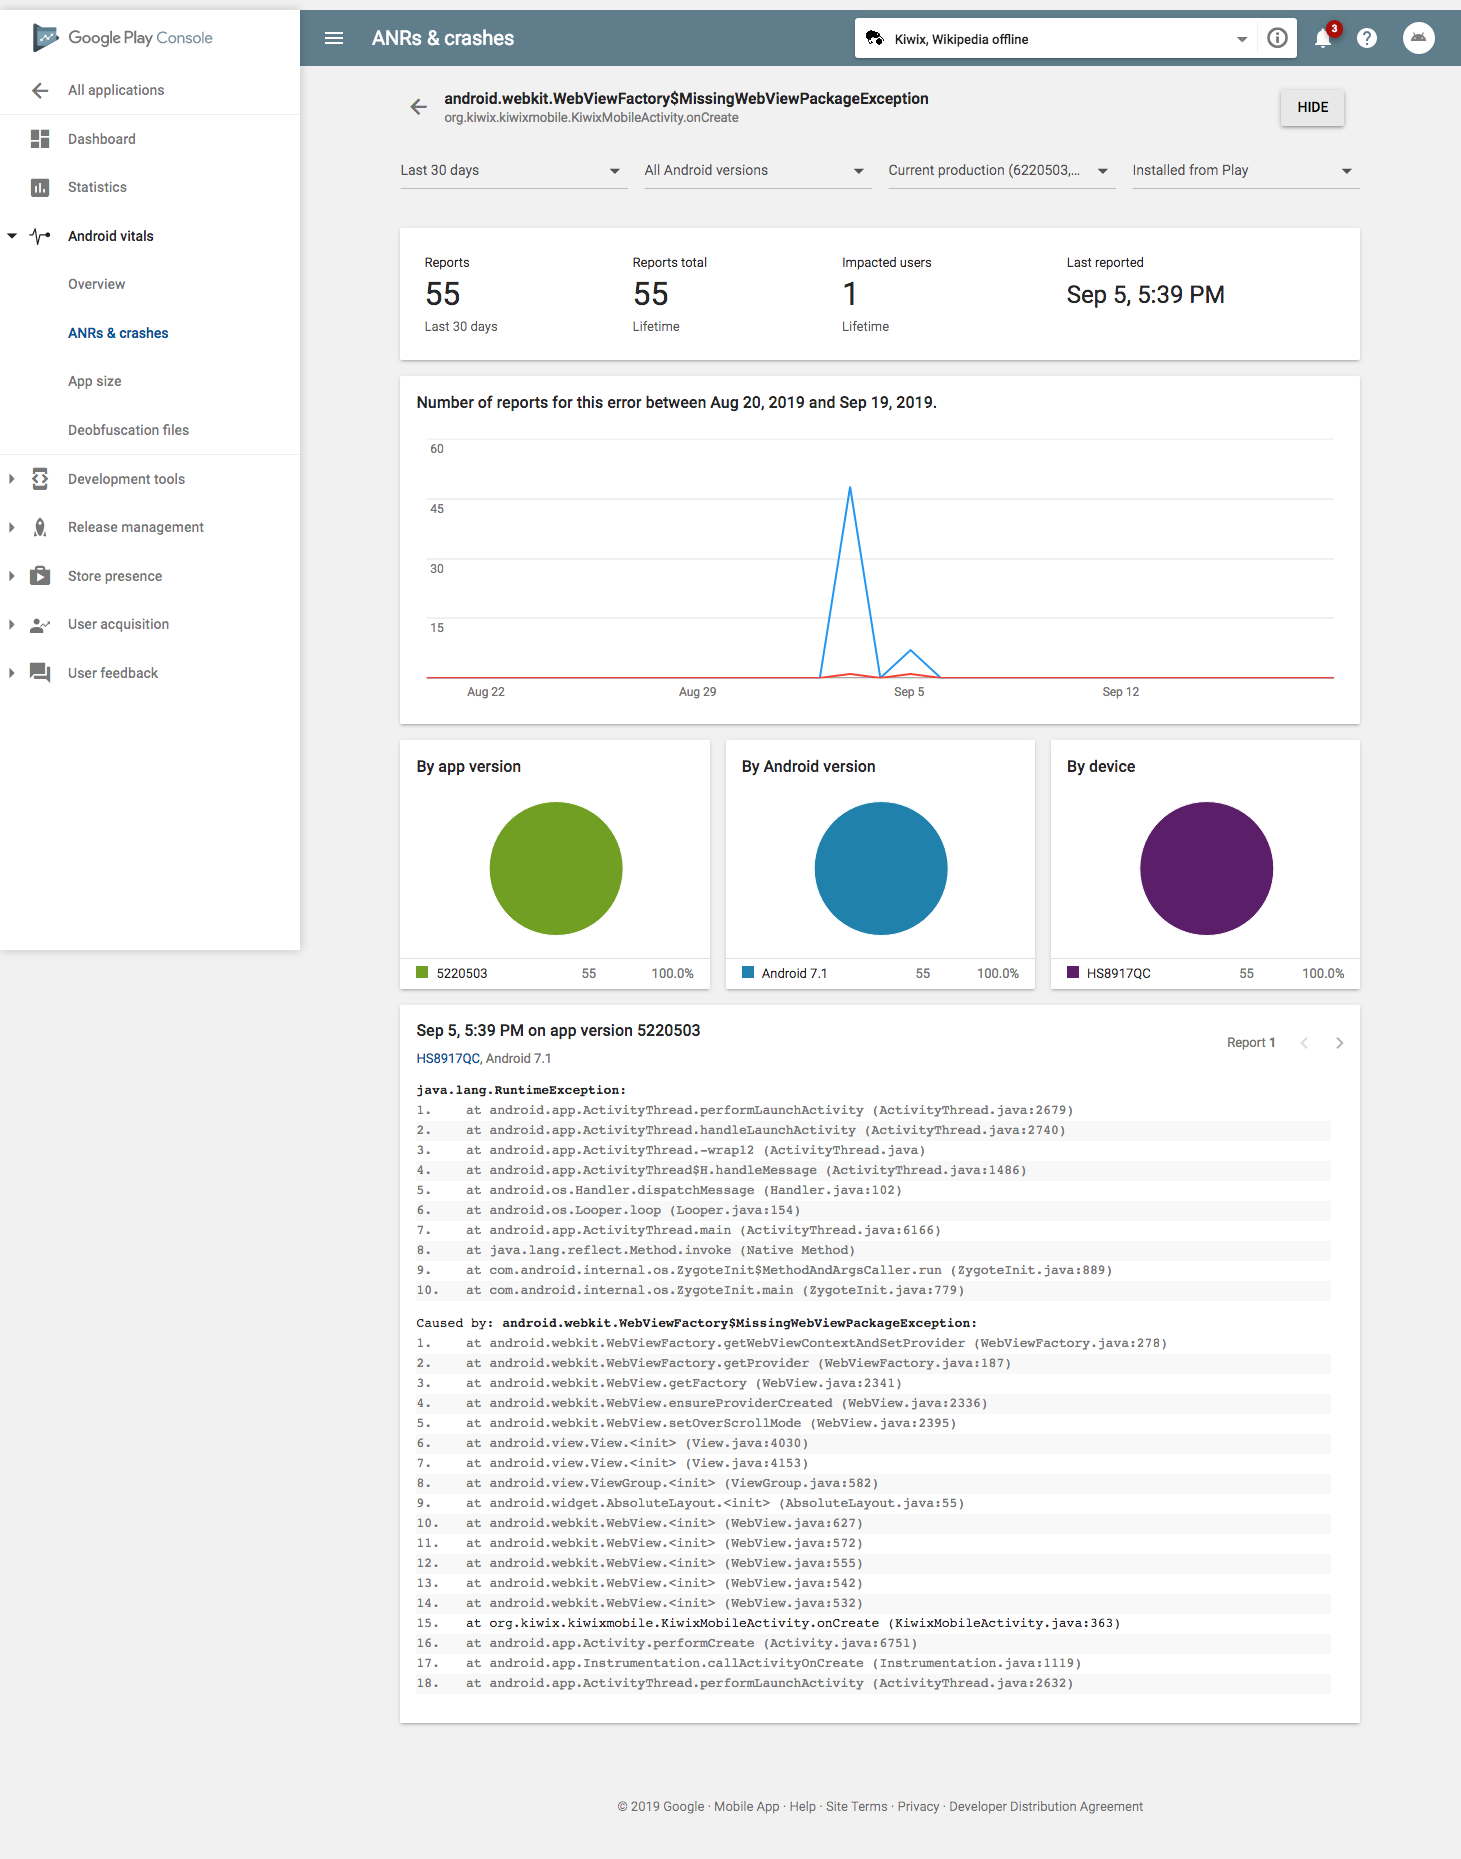
\includegraphics[width=14cm]{images/android-vitals-screenshots/55-crashes-WebViewFactory-MissingWebViewPackageException Screenshot_2019-09-19-kiwix.png}
    \caption{Google Play Console: Missing WebView Package Exception}
    \label{fig:55-crashes-missing-webview-package-exception}
\end{figure}

Another result from the paper is: \emph{"Given that the software is operating successfully, the chance of continued operation is greatly improved if there are only small changes in input conditions..."}. For mobile apps, one of the ongoing, major, sporadic changes are to the version of the operating system. As Linares \emph{et al} ~\cite{linares2013_api_change_and_fault_proneness_android} found, the most frequent cause of failure for Android apps is when the operating system is updated. Apps that were reliable on previous releases of the operating system may now start failing, and some failures become frequent and widespread as the new operating system release is adopted. \textbf{MUST-DO add evidence on the rollout and growth of Android releases in use as per old Google Android charts.}
~\yijun{This is very true in the TM352 I experienced. An argument may lead to the gap analysis is: how can one control or limit the effect of such external change factors or live with it? Is mobile analytics towards living with it while presenting an opportunity to spot such incompatibility issues earlier? }

These existing works help to establish the importance of reliability, some of the ways testing can be evaluated in terms of the subsequent reliability of the software in use, and some of the challenges in finding bugs that affect reliability. 

Another classic paper, from 1993, is by Musa~\emph{``Operational profiles in software-reliability engineering"}~\cite{musa1993_operational_profiles} which proposed using an operational profile to guide testing to maximise testing of the most-used operations. For mobile apps a key challenge, firstly there's unlikely to be a single operational profile for many apps given the variety of ways users use those apps how many would be needed to provide adequate coverage? and secondly where does the underlying information come from to determine what the operational profiles need to be in order to test effectively and efficiently? Musa does discuss ways to record the data: potentially Mobile Analytics may help to provide the data needed to establish these operational profiles? 

\textbf{TODO} sum up this section and connect it with Google's concept of Stability metrics to measure software quality for Android apps.

\subsection{Additional papers to consider on software quality}
These have not yet been incorporated into this section on Software Quality.
\begin{itemize}
    \item Sources of taxonomies and software testing include:~\cite{foidl2018_integrating_software_quality_models_into_risk_based_testing} 
    \item ``Cornering the Chimera"~\cite{dromey1996_cornering_the_chimera}.
    \item ``An Empirical Study on Quality of Android Applications written in Kotlin language"
    \item ``Mining Non-Functional Requirements from App Store Reviews"

\end{itemize}

\section{Measurement and Analytics}

\begin{figure}[!htbp]
    \centering
    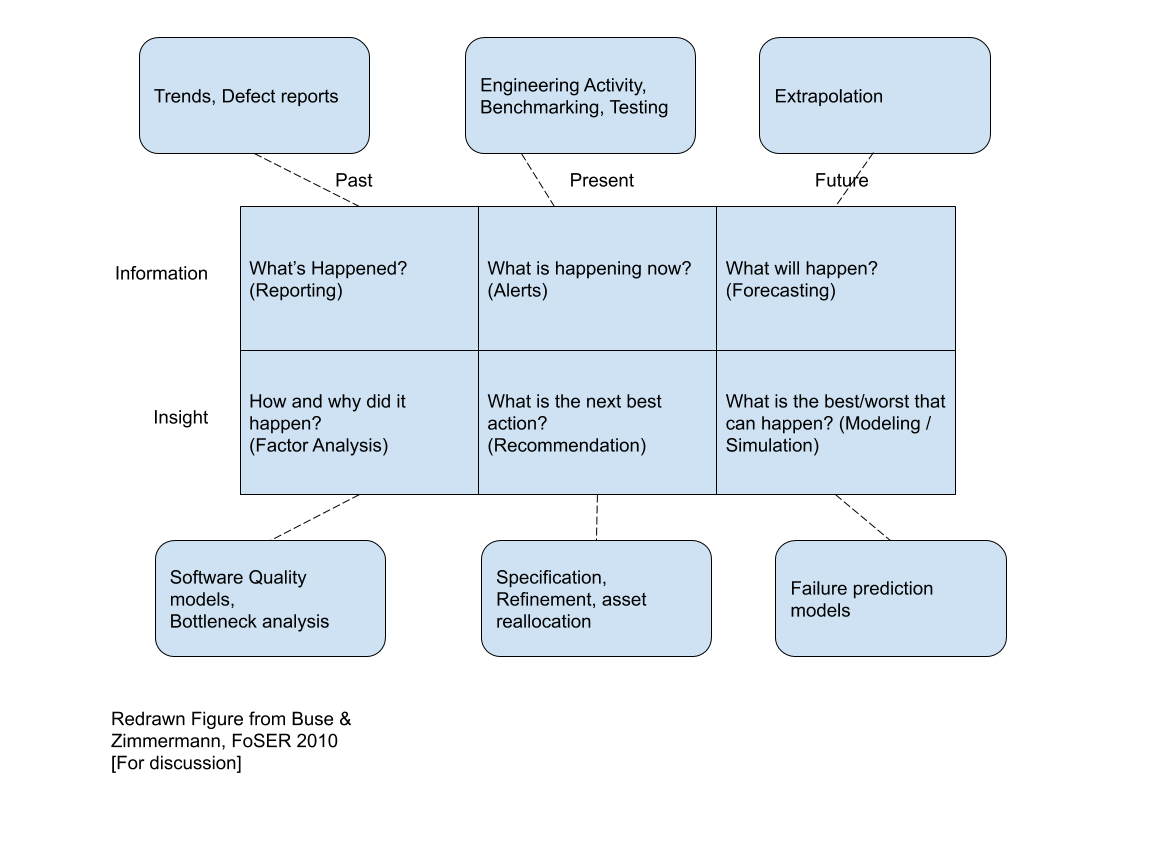
\includegraphics[width=14cm]{images/Buse_and_Zimmermann_2010_figure.png}
    \caption{Software Analytics, Buse and Zimmerman (2010)}
    \label{fig:software_analytics_buse_and_zimmerman_2010}
\end{figure}

Buse and Zimmerman wrote a short paper in 2010 which helped establish the field of:~\emph{``Analytics for Software Development"}~\citep{buse_analytics_2010}. The first figure in that paper is reproduced here as~\ref{fig:software_analytics_buse_and_zimmerman_2010}. They had derived that figure from a more general business-focused diagram in Davenport and Harris's book~\emph{``Analytics at work: Smarter decisions, better results"},  in Figure 1.1, titled\emph{``Key questions addressed by analytics"} and found in page 7 of ~\citep{davenport2010analytics_at_work}).

\begin{figure}[!htbp]
    \centering
    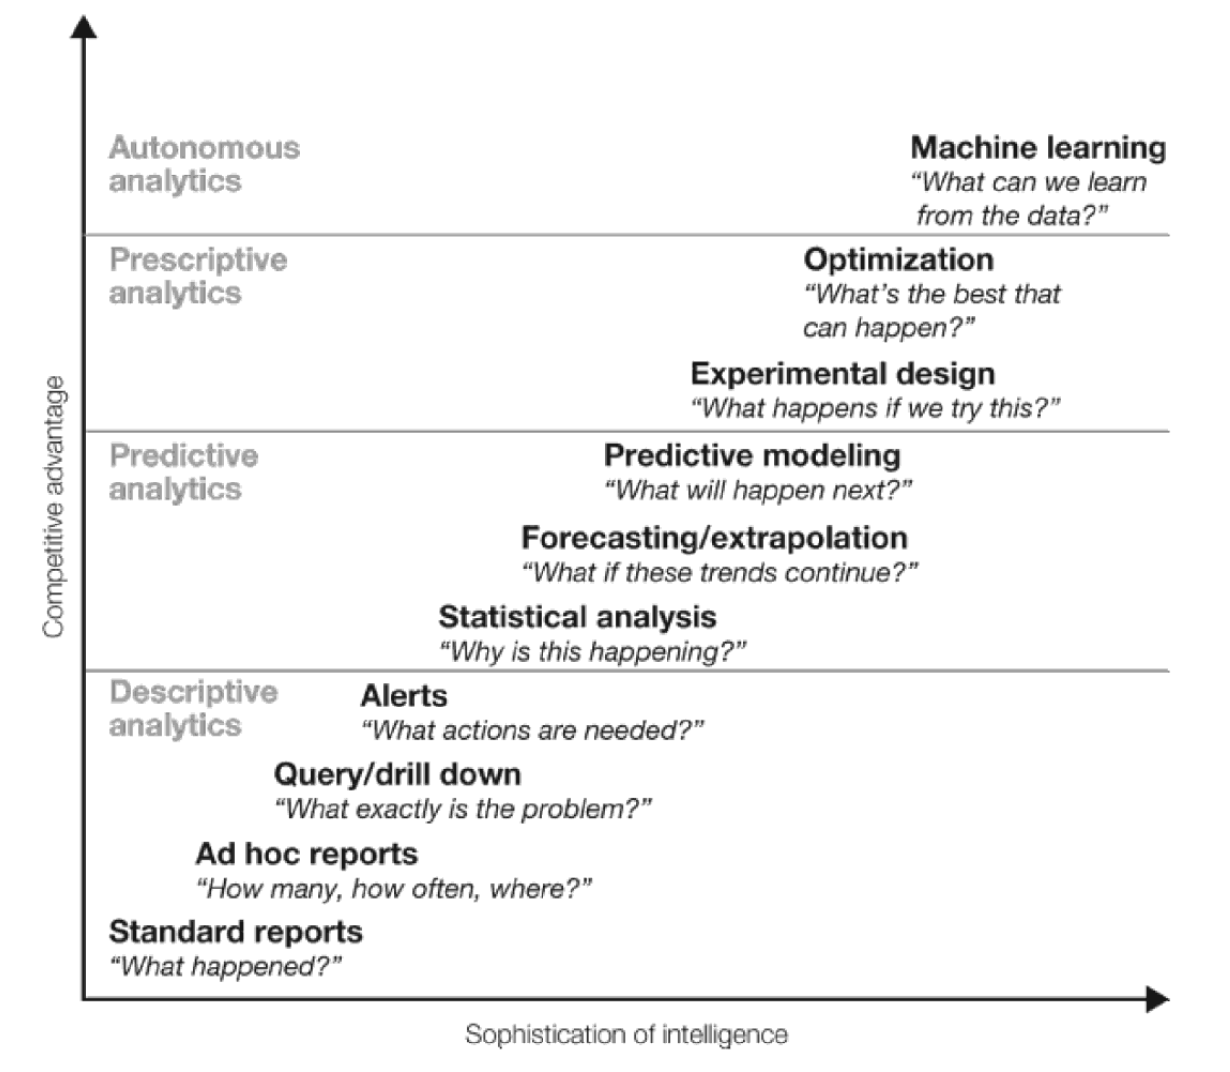
\includegraphics[width=14cm]{images/hbr/davenport-et-al-competing-on-analytics-2017-competitive-advantage.png}
    \caption{Davenport et al. Analytics for Competitive Advantage}
    \label{fig:davenport-analytics-for-competitive-advantage}
\end{figure}


\subsection{References/Sources to consider}
\begin{itemize}

    \item Davenport \textit{et al.} Competing on Analytics (\cite{davenport2017competing_on_analytics}) figure 1. Note: Google with version 4 of Google Analytics, launched in October 2020, are offering some machine learning based analytics to their customers, for instance to help marketeers... TBC. MUST-DO continue this topic and provide references to sources.
    
    \item Davenport \textit{et al.} Competing on Analytics (\cite{davenport2006competing_on_analytics}) that proposes several related functions: understanding customers and their contexts (including equipment and settings), product and service quality \emph{``detect quality problems early and minimise them"}, and to \emph{``improve quality, efficacy, and, where applicable, safety of products and services"}.
    
    \item \emph{Software Telemetry (MEAP)}~\citep{riedesel2020_software_telemetry_meap_v04}. An early draft of a book scheduled to be published in mid 2021 that discusses telemetry including the roots in system logs on early computer systems.
    
    \item Buse and Zimmermann...~\cite{buse_analytics_2010} 
    
    \item \emph{``Challenges and Benefits from Using Software Analytics in Softeam"} ICSEW 2020 \emph{``In this industry abstract, we describe the challenges and benefits of collecting feedback from customers and systems to support development cycles. In Softeam, we have performed such collection and support in four iterations by means of a software analytics platform. We describe the encountered challenges and the effects of suggested recommendations to improve the software quality of our systems on the metrics of interest."}~\cite{bagnato2020_challenges_and_benefits_from_using_software_analytics_in_softeam}. They use \url{https://github.com/q-rapids}, a ``Quality-aware rapid software development. H2020 Project (Grant no. 732253)". There are relevant publications listed at \url{https://www.q-rapids.eu/publications}.
    \item \emph{``"} \emph{``automatically collected usage data, logs, and interaction traces could improve feedback quality and help developers understand feedback and react to it. We call this automatically collected information about software usage implicit feedback."}~\citep{maalej2016_towards_data_driven_requirements_engineering}. They claim~\emph{``Thermal tracking of a user’s finger movement on touchscreens is a common approach for usage data analysis."} however I'm not aware of evidence to support this claim either from a research or a practitioner's perspective. (There's a PhD thesis on this topic published \emph{after} this paper: \href{http://usir.salford.ac.uk/id/eprint/37784/}{`Investigating the usability of touch-based user interfaces'}.
    
    \item ``A Methodology and Framework to Simplify Usability Analysis of Mobile Applications" Adding logging to a mobile apps can help developers analyse usability, reducing the effort needed
    
    \item \emph{``How Does Misconfiguration of Analytic Services Compromise Mobile Privacy?"} ICSE 2020. This in turn refers to \emph{``Alde: privacy risk analysis of analytics libraries in the android ecosystem."} 2016, and \emph{``Bug Fixes, Improvements, ... and Privacy Leaks - A Longitudinal Study of PII Leaks Across Android App Versions."} 2018.
    
    \item \emph{``Prochlo: Strong privacy for analytics in the crowd"}  ~\citep{prochlo2017_strong_privacy_analytics_in_the_crowd_46411} Various Google authors. 2017. Quote from the abstract:~\emph{``The large-scale monitoring of computer users' software activities has become commonplace, e.g., for application telemetry, error reporting, or demographic profiling. This paper describes a principled systems architecture---Encode, Shuffle, Analyze (ESA)---for performing such monitoring with high utility while also protecting user privacy. The ESA design, and its Prochlo implementation, are informed by our practical experiences with an existing, large deployment of privacy-preserving software monitoring."}.

    \item "QoE Doctor: Diagnosing Mobile App QoE with Automated UI Control and Cross-layer Analysis"~\cite{chen2014qoe}.
    \item "An Approach to Detect Android Antipatterns"~\cite{hecht2015approach}. Using static analysis to find poor designs that lead to poor quality apps. Their approach could be complementary to mine and to ... software testing.
    \item ``Examining the Relationship between FindBugs Warnings and App Ratings"~\cite{khalid2016_examining_the_relationship_between_findbugs_warnings_and_app_ratings} assessed the static-analysis warnings collected using FindBugs with ratings and the associated review comments for 10,000 free-to-download Android apps.
    
    \item \emph{``Apps, Trackers, Privacy, and Regulators: A Global Study of the Mobile Tracking Ecosystem."} 2018
    
    \item \emph{``Continuously assessing and improving software quality with software analytics tools: a case study"}~\cite{martinez_fernandez2019_continuously_assessing_and_improving_software_quallty_with_software_analytics_tools}.
    
    \item \emph{``Toward a learned project-specific fault taxonomy: application of software analytics"}~\cite{kidwell2015_toward_fault_taxonomy_application_of_software_analytics}.
    
    \item \emph{``A measurement study of tracking in paid mobile applications"}~\citep{seneviratne2015_a_measurement_study_of_tracking_in_paid_mobile_apps}. Of the trackers this paper identified, 14\% of paid apps and 11\% of free apps used trackers that provided utilities such as crash and/or bug reporting and 28\% of paid apps and 24\% free apps used trackers that provided analytics (some of these also collected information on crashes). Their process was quite involved in order for the researchers to identify the trackers, currently (in 2021) various online services including the exodus-privacy~\citep{exodus_privacy_project} and AppBrain~\citep{appbrain} provide such information for Android apps freely. Virtually everyone of the 300 participants' devices had at least one tracker incorporated into at least one app on their device. 50\% of the users had more than 25 trackers. Therefore, this research confirms tracking in mobile apps is endemic and has been performed for years. 
    
    \item \emph{``User interaction-based profiling system for Android application tuning"}~\citep{lee2014_user_interaction_based_profiling_system_for_android_app_tuning} Correlation or causation, needing to investigate... I've discussed one of their figures in many presentations on Mobile Analytics. To be continued...
    
    \item \emph{``A Recipe for Responsiveness: Strategies for Improving Performance in Android Applications"}~\citep{nilsson2016_a_recipe_for_responsiveness_for_improving_android_apps_spotify_masters} presents some of the challenges of measuring and improving the performance of a particular, very popular Android app: Spotify~\footnote{\href{https://play.google.com/store/apps/details?id=com.spotify.music&hl=en_GB&gl=US}{Spotify: Free Music and Podcasts Streaming}.}. Several of the measurements described in the paper were later integrated into Google Play Console's Android Vitals service. The author created an additional tool that profiles the performance of UI elements and provided the results as three traffic-light indicators for: Draw, Layout, Execute. The work was well received within Spotify, however as the tool was not applied to other apps and is not available the impact of this research seems to be limited.
    
\end{itemize}

\subsection{Topics to mention}
\begin{itemize}
    \item Use of analytics is ubiquitous by software, including operating systems (e.g. OSX), mobile platforms (including Android and iOS), web servers, and mobile apps. 
    \item Understand what's being measured, and what's being claimed. e.g. Zoom corrected their claims about their user-base for their progress report on \nth{22} April 2020 \emph{even with more than 300 million daily meeting participants.}, they acknowledged they'd previously stated the claimed meeting participants were users and people \emph{"Edit 4/29/20: This blog originally referred to meeting participants as “users” and “people.” This was an oversight on our part."}~\footnote{~\url{https://blog.zoom.us/wordpress/2020/04/22/90-day-security-plan-progress-report-april-22/} and see the commentary in the ITPro article:~\url{https://www.itpro.co.uk/marketing-comms/communications/355498/zoom-quietly-corrects-misleading-claims-of-over-300-million}}
    \item Ways data can be used
    \item Privacy, and who is responsible for the data being collected, shared, and protected?
\end{itemize}

Integrated metrics and data about software development projects: dashboards such as~\href{https://bitergia.com/bitergia-analytics/}{Bitergia Analytics} and an online live example of their dashboard~\url{https://onap.biterg.io/app/kibana#/dashboard/Overview?_g=()} aim to provide a holistic view to software development teams of data that matters to them. 
GrimoreLab~\url{https://chaoss.github.io/grimoirelab/} is used to build various projects including the Bitergia Analytics Platform and~\href{https://cauldron.io/dashboard/1640}{Cauldron.io}. It includes support for a wide variety of data sources (source code management, issues/task management, source code review, mailing lists and forums including stack overflow, continuous integration, synchronous communications, wikis, meeting management, and others). What it does not current support are any analytics data sources which means developers have to look elsewhere and use other tools and dashboards to obtain analytics about how their software is performing and behaving. 


% MUST-DO I may need relocate the following paragraphs again, they seem to belong a bit better here than earlier. The idea is to introduce the concept of ways several quality aspects can be measured.
Nonetheless, several facets are able to be tracked remotely for mobile apps, an important factor in terms of the ability to facilitate practical approaches aimed at developers of these apps. They can be collected with various degrees of automation and to varying degrees, for instance the time something takes can be recorded at a micro level for a few lines of source code and at a macro level at the app or device level and across many devices and apps. 

There are well-established tools, techniques and practices for recording the time taken. Many of the tools are suited to use locally and directly by a developer, including Memory, App, and Network Profilers~\footnote{\url{https://developer.android.com/studio/profile\#android-studio-tools}}.For remote measurements the tools include Google's Android Vitals and Firebase Performance Monitoring\footnote{\url{https://firebase.google.com/docs/perf-mon}}.

User experience (UX) can be assessed using a wide variety of tools and techniques, such as heatmapping (which uses screen and/or interaction recording), A/B testing frameworks, funnel and journey analytics, and so on. By their very nature they're user-focused and - in practice - seldom incorporated into mobile apps or development practices for mobile apps. Similarly, based on my investigations, they are seldom researched although I have co-written work on this topic including examples of using heatmapping to improve usability of mobile apps~\cite{harty_aymer_playbook_2016}.

\subsection{Development Logging}
Consider a 2D matrix of use of logging (amount, choice of library and API, formatting and customisation), and the range of the logging (local<->logging at a distance). Papers such as \emph{A Methodology and Framework to Simplify Usability Analysis of Mobile Applications}~\url{https://doi.org/10.1109/ASE.2009.12}. Remember to cover this topic in the work we did on logging (And the recent Shonan work). Mention the Shonan workshop in this section too.

\subsubsection{Use of logging}

Where Shall We Log? Studying and Suggesting Logging Locations in Code Blocks~\cite{li2020_where_shall_we_log}, costs of logging (and discuss data leakage and loss of privacy).


Where to log and what to log... Where to log has been researched by various authors. \cite{li2020_where_shall_we_log} identify six categories of logging locations in several mature opensource codebases, used in domains outside mobile apps. Research into where logging statements are added in large-scale industrial codebases are covered in various papers including:~\cite{zhu2015_learning_to_log} where a \emph{`Log Advisor'} made recommendations of where to log to developers, they excluded the contents of the log messages from their research and their log advisor as too difficult to address in the scope of their work at the time.

What to log depends materially on the context of intended use of the contents of the log messages. For example, logging data generated by smartphones can log details of when and how users use their devices~\citep{ormen2015_smartphone_log_data_qualitative_perspective}. The authors identified a key challenge beyond what to log was the interpretation of the contents, and in their small scale qualitative study involving 12 subjects they supplemented the log data with interviews - something relatively easy to do as the subjects were known and active participants in the research, and impractical for the vast majority of app developers who have orders of magnitude more users where the users and developers do not know each other.




\subsubsection{Research in logging}
\textbf{SHOULD-DO} \emph{``Identifying Impactful Service System Problems via Log Analysis"} Temporary link:~\url{https://doi.org/10.1145/3236024.3236083}. There's a good review of this paper at~\url{https://blog.acolyer.org/2018/12/19/identifying-impactful-service-system-problems-via-log-analysis/}, and the code is opensource at \url{https://github.com/logpai/Log3C}.


\subsubsection{Designing logging}

\subsection{Ubiquitous Analytics}
After OSX operating system updates, and when new users first login, they are asked to "help app developers improve their products and services automatically." Tickbox, default un-selected: "Share crash and usage data with app developers", "Help app developers improve their apps by allowing Apple to share crash and usage data with them." Further details, including from a user's perspective what's collected, how long the data is kept, and how to disable diagnostics from being sent are all described in \url{https://support.apple.com/en-gb/guide/mac-help/mh27990/mac}

\subsection{Ways data can be used}
In Industry there are discussions on various ways data can be used to get the most out of the data. Figure~\ref{fig:i_am_using_data_to} presents a decision tree discussed in an article on when to apply each perspective~\cite{amplitude_are_you_data_driven}. For my research, and for development teams who use analytics, we may choose to use these various perspectives to use analytics data more productively. This work leads to the question of identifying and often designing the data that will need to be collected in order to use it.

\begin{figure}[!htbp]
    \centering
    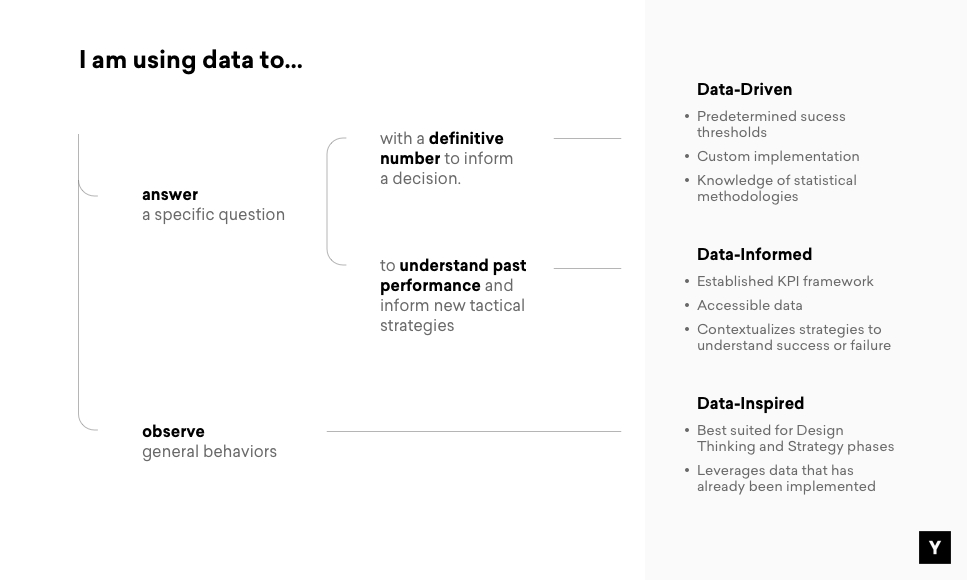
\includegraphics[width=15cm]{images/data-informed-graphic-ymedia-labs.png}
    \caption{I am using data to... (from Y Media Labs)~\cite{amplitude_are_you_data_driven}}
    \label{fig:i_am_using_data_to}
\end{figure}
%First discovered via \url{https://twitter.com/iteratively/status/1243641701408935936?s=20}

% SHOULD-DO write about: Identifying and designing data....

In a short paper~\citep{kidwell2015_toward_fault_taxonomy_application_of_software_analytics}, the authors propose combining fault classification and software analytics for five types of decisions. These are: targetting testing, release planning, judging stability, targeting training, and targeting inspection of software. failure data mined from software analytics tools such as crash reporting tools helps to bring their concepts and ideas to life. Their paper provided initial indicative evidence of their proposals through evaluation of changes to source code for the Eclipse software and discusses the measurement of refactoring to provide more accurate and relevant measurements of the efficacy of the refactoring, rather than considering approaches to improve mobile apps.

\subsection{Privacy and Control}

UW blog post~\cite{mcquate_I_saw_you_were_online} and the underlying CHI 2020 paper~\cite{cobb2020_ux_s_with_online_status_indicators} regarding how online status indicators shape their behaviour and on whether people know and can correctly control whether their data is being shared. Conversely, in his PhD thesis~\citep{adam2009balancing}, Adam noted that users of mobile devices were willing to withhold sensitive data provided they would not be found out. The users want blameless ways to control their privacy.

Mobile analytics collects a time-series of data online. In 2015, research into privacy concerns of continual observation identified a number of concerns with the erosion of privacy for users in these circumstances~\citep{erdogdu2015_privacy_utility_tradeoff_under_continual_observation}. The authors discussed various end-user concerns in having to trust the collection of their user data, including two trust boundaries: either locally, where~\emph{``the user may not entirely trust the aggregating entity in the first place,"} or at the aggregator's side - where the user trusts the entity collecting the data but not third-parties who may also gain access to the data. Either or both of these concerns may apply when users use mobile apps that collect analytics data. Their experiment that assessed whether six households could keep private their use of a microwave while simultaneously sharing data that enabled their washer-drier usage to be accurately tracked. Given the small-scale nature of the experiment it would be premature to determine whether the framework proposed in the research would also apply to mobile analytics, nonetheless the research offers a possible approach to increasing the privacy of mobile analytics data provided the data is still efficacious and sufficiently accurate for diagnostics, problem analysis, and reporting purposes.  

% Further reading
% https://www.kaggle.com/dansbecker/what-is-log-loss (refreshingly clear and succinct, I still don't quite understand the topic yet though...)
% A great title, I wish I understood the topic: "From the Information Bottleneck to the Privacy Funnel". Also their approach is unlikely to be used in mobile analytics software as there's little perceived practical need to provide privacy of this form :( 

% The purpose driven privacy preservation for accelerometer-based activity recognition 
The tradeoff between privacy and utility for data that can uniquely identify over 99\% of users from high-frequency data collection from accelerometers in mobile phones~\citep{menasria2018_purpose_driven_privacy_preservation_accelerometers}. Accelerometer data is one class of data that could be collected using mobile analytics. The paper discusses the compression of data that is disclosed so irrelevant private information can be reduced while also maintaining adequate utility of the analysis of the data that is disclosed. Their approach might offer the potential to reduce irrelevant private information collected by mobile analytics.

Privacy related violations by platform providers, including Apple and Google, where a user's phone (and presumably similar devices including tablet computers) are tracking users without the user's informed consent. A recent complaint was filed by NOYB - European Center for Digital Rights~\citep{noyb2020_noyb_files_complaint_against_apples_tracking_code_idfa} and reported by the Financial Times~\citep{ft2020_apple_tracks_iphone_users_without_consent}. The complaint is that iPhones track users and Apple shares the data with all the app developers. According to the article in the Financial Times, in June 2020 Apple promised their latest operating system, iOS14, would include a privacy dashboard and that apps would need to ask users for permission before accessing the unique IDFA (Identifier for Advertisers). However, again in this article~\emph{``Apple then said in September that it would delay the changes, “to give developers the time they need” until “early next year”."}. 



c.f. using infra-red cameras to detect people in ways they're unfamiliar with and do not expect. 

\section{Software Development Practices}

Topics include: Agile development and the effects of the software that's developed and released. Motivations for/of software developers.

\subsection{Papers to consider on software development practices}
\begin{itemize}
    \item \emph{A systematic review of theory use in studies investigating the motivations of software engineers}~\citep{hall2009systematic}.
    \item \emph{Designing Engineering Onboarding for 60+ Nationalities}~\citep{harty2020_designing_engineering_onboarding}. Onboarding software developers and staff generally also includes exceptions and exception handling. These exceptions can be collected and analysed to determine where the onboarding is failing. Again there can be the concept of non-fatal and fatal exceptions. Fatal exceptions shouldn't happen ideally, there are mechanisms to handle them adequately in terms of error recovery, however we'd like to know about them and address them.
    \item \emph{Enabling Productive Software Development by Improving Information Flow}~\citep{murphy_enabling_2019}. 
    \begin{itemize}
        \item ``The flow of information among software developers is directly related to productivity."
        \item ``When the flow of information is adequately supported, delivery times on software can be shortened, and productivity within an organization can rise."
    \end{itemize}
    \item \emph{Continuous delivery sounds great, but will it work here?}~\citep{humble2018_continuous_delivery_sounds_great}. 
    \begin{itemize}
        \item ``Continuous delivery is about reducing the risk and transaction cost of taking changes from version control to production. Achieving this goal means implementing a series of patterns and practices that enable developers to create fast feedback loops and work in small batches. This, in turn, increases the quality of products, allows developers to react more rapidly to incidents and changing requirements and, in turn, build more stable and higher-quality products and services at lower costs."
        \item ``If this sounds too good to be true, bear in mind: continuous delivery is not magic. It's about continuous, daily improvement at all levels of the organization—the constant discipline of pursuing higher performance. As presented in this article, however, these ideas can be implemented in any domain; this requires thoroughgoing, disciplined, and ongoing work at all levels of the organization. Particularly hard, though essential, are the cultural and architectural changes required."
    \end{itemize}
    
\end{itemize}


\section{Software Testing}

\subsection{Papers to consider}
\begin{itemize}
    \item TBC
    \item \emph{``Debugging without testing"}~\cite{ghardallou2016debugging_without_testing} It may be possible to demonstrate a bug has been fixed without testing, for instance by comparing behaviours before and after changes were made to the software. This paper's premise of being able to debug without testing held true in some of my research. Testing has not able to reproduce all the conditions needed for some bugs to emerge. Other information, such as stack traces, may help developers perceive likely causes of a bug, such as a crash, sufficiently for the developers to take what they believe is corrective action.  
    
    \item ~\emph{`Communication in Testing: Improvements for Testing Management'}~\citep{paakkonen2009_communication_in_testing}: 
    \begin{itemize}
        \item Three quality approaches: mapping of process, product, and quality-in-use => three perspectives: software engineer (developer), testing, and end-user. The first two are easier to measure for a software company, yet the quality-in-use is the most important for any product. \textbf{TBC}
    \end{itemize}
    
    \item Behaviourally Adequate Software Testing \url{https://leicester.figshare.com/articles/Behaviourally_Adequate_Software_Testing/10106189} - Behavioural Coverage, search-based white-box generation strategies. Measures of testing adequacy. \emph{One intuitive notion of adequacy, which has been discussed in theoretical terms over the past three decades, is the idea of behavioural coverage; if it is possible to infer an accurate model of a system from its test executions, then the test set must be adequate.} IIRC the programs they assess are tiny, and how can we determine 'accurate model', perhaps it'll be accurate for what it tests, but incomplete? "The truth, \emph{the whole truth}, and nothing but the truth" springs to mind. % See also Uncertainty-Driven Black-Box Test Data Generation (seems less relevant to my research) and Assessing Test Adequacy for Black-Box Systems Without Specifications (perhaps more relevant).
    
    \item Various papers listed on \url{https://testroots.org/publications.html} which focus on IDE measurements of developers running automated tests, CI and tests~\emph{``Oops, My Tests Broke the Build: An Explorative Analysis of Travis CI with GitHub"}, and code quality correlations between test and system code.
    
    \item "Probably approximately correct learning" however it seems to be unrealistic and impractical for shipping mobile app development teams.
\end{itemize}


\subsection{Concepts to consider}
\begin{itemize}
    \item Adequacy
    \item Confidence levels (in the testing we've done)
    \item Sufficiency (c.f. how Google graded OKRs where 0.7 was the expected, sufficient, amount of progress).
    \item What testing actually gets done for real software, rather than what testing standards, academia, etc. tells us we \emph{should} do.
    \item Probably Approximately Correct.
    \item Testing logging and analytics, especially when many aspects of the systems are provided by third-parties, involves determining causal links between two phenomena. Concommitant variations, introduced in~\cite{mill1884system}
    \item Who tests the software developers use? for instance the many APIs and libraries? Flaws in this software, created by others, may affect the development teams and the users of their software products, amongst others. This software will include proprietary code and will probably include opensource code, perhaps pre-packaged as libraries of binary code. Some of that software may be poorly maintained, and yet the quality of that software may adversely affect the quality of the code using it. 
\end{itemize}

\section{App Stores and their Effects on Software Development and Engineering}
The concept of an App Store has existed since at least 2003, according to the co-founder and CEO of Salesforce~\cite{benioff_trailblazer_2019}, where the idea was proposed by Steve Jobs and later implemented as \href{https://appexchange.salesforce.com/}{\emph{AppExchange}} in the Salesforce platform. Around the same period various app stores emerged for mobile apps~\footnote{Tens of app distribution platforms are listed on Wikipedia:~\href{https://en.wikipedia.org/wiki/List_of_mobile_app_distribution_platforms}{List\_of\_mobile\_app\_distribution\_platforms}}; and the concept seems to have been introduced around 1999 by Handandgo~\footnote{\url{https://en.wikipedia.org/wiki/Handango}}. Academic research into the effects of app stores emerged in or around 2010, for instance with the work of Kimbler who investigated the effects on mobile operators from a business strategy perspective~\cite{kimbler_app_store_strategies_2010} (who lost out in the overall battle of app stores, now platform specific app stores dominate the market). 

Also in 2010, early papers were published on various effects of app stores on academic research e.g. how app stores addressed some of the previous constraints such as reaching more users and facilitating the distribution of the apps and feedback from those users~\cite{cramer2010_research_in_the_large_app_stores, miluzzo2010research_in_the_app_store_era}. 

\begin{itemize}
    \item Cramer \emph{et al} discussed aspects of \emph{research in the large} and in particular for my research the importance of ``playing by the rules"~\cite{cramer2010_research_in_the_large_app_stores}. My research was also shaped to play by the rules of the app store.

    \item Miluzzo \emph{et al} introduced other relevant research aspects, \textit{i.e.}  ongoing concerns such as how to assess correctness when there is no \emph{``ground truth"} - a challenge when evaluating mobile analytics for shipping apps; and a software development model of \textit{``deploy-use-refine"}~\cite{miluzzo2010research_in_the_app_store_era}, where app development refines the app based on data gleaned from usage of the app. Our case studies used usage data to refine the app to improve the measured reliability of the apps. Their paper even explained how a silly mistake caused their app to crash where the app store then delayed the new release of the app by several weeks. Even in 2010 crashes adversely affected the app store's perception of an app. % Their work on CenseMe received an ACM Test of Time award, see https://www.cs.dartmouth.edu/~campbell/page-3/
\end{itemize}

\subsection{Papers to consider}
\begin{itemize}
    \item \emph{``App store effects on software engineering practices"}~\citep{alsubaihin2019app_store_effects_on_software_engineering}
    
    \item \emph{``A survey of app store analysis for software engineering"}~\cite{martin2016survey, martin2017_survey_in_app_store_analysis_for_software_engineering_IEEE_edition}.
    
    \item \emph{``Why people hate your app: Making sense of user feedback in a mobile app store"}~\cite{fu2013people}. A key paper, many citations (some also highly relevant).
    
    \item \emph{``Analyzing and Automatically Labelling The Types of User Issues that are Raised in Mobile App Reviews"}~\cite{mcilroy2016analyzing} - discusses crashes, crash libraries, analytics, relatively early paper on the topic.
    
    \item \emph{``Revisiting the Mobile Software Ecosystems Literature"}~\cite{steglich2019revisiting} Helps to define what an ecosystem is.
    
    \item \emph{``Beyond Google Play: A large-scale comparative study of Chinese Android app markets"}~\cite{wang2018_beyond_google_play}.
    
    \item \emph{``Measurement, modeling, and analysis of the mobile app ecosystem"}~\cite{petsas2017measurement}.
    
    \item \emph{``A Measurement-based Study on Application Popularity in Android and iOS App Stores"}~\cite{liu2015measurement}.
    
    \item \emph{``Understanding the Evolution of Mobile App Ecosystems: A Longitudinal Measurement Study of Google Play"}~\cite{wang2019understanding} (2019): Lots of interesting questions and observations about Google Play; but they don't seem to consider flaws, or the effects of flaws, in the app store's data collection, algorithms, etc.
    
    \item \emph{``Release Practices for Mobile Apps--What do Users and Developers Think?"}~\cite{nayebi2016release}.
    
    \item \emph{``Towards Release Strategy Optimization for Apps in Google Play"}~\citep{shen2017_towards_release_strategy_optimization_for_apps_in_google_play}. ``empirical study to help developers decide the release opportunity to maximize positive feedback from users at scale.". They identify three patterns of update intervals: successive, normal, sparse. Their work does not use signals such as the stability of the app. They also claim ``Additionally, app quality can be unstable with fast [release] iteration[s]."
    
    \item \emph{``Feature lifecycles as they spread, migrate, remain, and die in App Stores"}~\cite{sarro2015_feature_lifecycles_in_appstores} discusses \emph{adaptive development} as a concept for developers of apps in app stores. Notes: Their research is based on `non-free features from two app stores (Samsung and Blackberry)' (both relatively dwarfed by Google Play) and their work predates the availability of platform level analytics, etc. Relevance to my work: developers can obtain requirements (in terms of work they're potentially `required' to do) from many sources, including direct feedback from end users of the apps, signals in terms of willingness to install and keep using their app, and from analytics. Developers want and increase the value of their work by prioritising potential work appropriately. Signals and data from mobile analytics may provide useful, additional sources of information that's sufficiently relevant for developers to accept these `requirements' and address them.
    
    \item \emph{``Which version should be released to app store?"}~\cite{nayebi2017version}.
    
    \item \emph{``Modern release engineering in a nutshell - why researchers should care"}~\cite{adams2016modern}.
    
    \item The \emph{``Data analytics for decision support in software release management"}~\cite{didar2018data_analytics_phd_thesis}, a PhD thesis, introduces a proposed Plan-Monitor-Improve Framework for release management.
    
    \item \emph{"An Explorative Study of the Mobile App Ecosystem from App Developers' Perspective"}~\cite{wang2017_exploratory_study_of_the_mobile_app_ecosystem}: 1,000,000+ apps on Google Play, 320,000 developers, over half of the developers only released a single app. The paper mainly focuses on the \emph{"the group of aggressive developers who have released more than 50 apps, trying to understand how and why they create so many apps"}. Provides some context on who writes the mobile apps in Google Play, provides an estimate of the population of developers (in 2017).
    
    \item \emph{``Requirements Intelligence: On the Analysis of User Feedback"}~\cite{stanik2020requirements_intelligence_on_the_analysis_of_user_feedback}. continuous sources for requirements-related information; comparison between explicit and implicit user feedback (like app usage data).
    
    \item \emph{``Are apps ready for new Android releases?"}~\cite{guilardi_are_apps_ready_for_new_android_releases}. A current (2020) paper where the researchers discovered that developers are slow to revise and update their Android apps for new releases of the operating system. Some of the apps have flaws exposed when running on new versions of the operating system. For apps to retain their quality they need to be updated, new releases of the operating system are one such reason. (Releases of libraries another, new contexts of use, etc. another...).
    
    \item \emph{``Revisiting Prior Empirical Findings For Mobile Apps: An Empirical Case Study on the 15 Most Popular Open-Source Android Apps"}~\citep{syer2013_empirical_findings_for_mobile_apps} is work from 2013 (when Google Code was still a major active public source code repository) that compares the codebases of 15 opensource mobile apps with 5 other opensource desktop/server projects. A key finding in their research includes the development process - where there are frequent releases yet the development and release processes are immature. albeit based on codebases from 2011 so a decade ago is still relevant. They ask various open-ended questions:
    \begin{itemize}
        \item Does such a high frequency of releases mitigate the lack of testing? 
        \item If there are frequent releases for the mobile app, then does quality matter as much?
        \item Is the project in a constant beta testing state? 
        \item Does the platform provide sufficient support for building high quality apps quickly? 
        \item Is the frequent release only influenced by the demand factor in the app store? 
        \item Are the developers of mobile apps more skilled or do they have more resources at hand? 
        \item Or, are mobile apps themselves less complex to develop?
    \end{itemize}
    
    Perhaps the cost of failures in the app store was/is perceived to be low in the Google Play app store, at least for these 15 opensource apps? Later work investigated aspects such as the release frequency~\citep{nayebi2016release}
    
\end{itemize}


App Stores behave as intermediaries between developers and the users of their software. They make various aspects more transparent including pricing, information about the apps, releases, and ratings \& reviews. There are hundreds of thousands of developers of Android apps according to various sources (320,000 in 2017~\cite{wang2017_exploratory_study_of_the_mobile_app_ecosystem}, ...).


In an App Store first the developer then the app store are involved in making a release available to some or all of the user population. There are various competing factors that affect when would be a good time to make a release. Too few and an app may be considered stale or neglected, too many and users may balk at the seemingly endless updates and communications costs. Groups of researchers have investigated various aspects of release engineering, including~\cite{adams2016modern} that argues the relevance of modern release engineering and the relevance for researchers, and~\cite{nayebi2017version} which concentrates on which version of opensource apps should have been released to the app store. Developers, and their stakeholders, want to make more informed decisions about which releases to make; however there does not appear to have been much research into the testing and quality indicators available to app developers before they make their release public.


\section{Developing Mobile Apps}

\subsection{Papers to consider}
\begin{itemize}
    \item TBC
    \item \textbf{Species of Bugs}
    \item J2ME write once debug on a million devices quote?
    \begin{itemize}
        \item \emph{``Finding resume and restart errors in Android applications"}~\cite{shan2016finding}. Which leads to "Large-scale analysis of framework-specific exceptions in Android apps" (2018) where the exceptions should be detectable by Android Vitals, I hope.
        \item \emph{``JInjector"} the makeup of mobile apps~\citep{sama2009using_jinjector}. \emph{``Statistically most of the code in a J2ME application belongs to the GUI;"}. The tool was also applied to Android apps and provided similar capabilities to instrument the GUI. Null Pointer Exceptions (which affect both Android Java apps and J2ME apps) can elude the development and testing pre-release of apps, even from Google-calibre software engineers. Freezing in J2ME apps were also detected, and freezing is one of the factors measured by the Android platform and reported as ANRs.
        \item \emph{Do android developers neglect error handling? a maintenance-centric study on the relationship between android abstractions and uncaught exceptions}~\citep{Oliveira_Borges_Silva_Cacho_Castor_2018_android_error_handling}.
    \end{itemize}
\end{itemize}




\subsection{Bugs}
Species of bugs: inadequate and neglected error handling, data loss bugs.

Exception handling is strongly related to program robustness.~\citep{Oliveira_Borges_Silva_Cacho_Castor_2018_android_error_handling}. In particular, they observed that developers did not write sufficient code to handle exceptions that could be thrown when their Android app uses Android-specific abstractions. Uncaught exceptions lead to the application crashing, and crashes are an indication of poor reliability of the application. Of course, the exception needs to occur in order for the app to crash, and not every uncaught exception causes the app to crash, they may crash an internal thread within the app instead~\citep{Oliveira_Borges_Silva_Cacho_Castor_2018_android_error_handling}. %Note: not all caught exceptions are handled adequately. E.g. some may simply be logged and the code allowed to continue unchanged. Sometimes the exception may mean internal state and/or data are incomplete or incorrect for reliable and correct operations of the app. 
Their research excluded various factors that also affect robustness, in particular they chose not to study: ``security vulnerabilities, excessive resource consumption, and race conditions."~\citep{Oliveira_Borges_Silva_Cacho_Castor_2018_android_error_handling}. %As an observation, they appear to over-state the LOC they analysed, or at least they're inflating the counts to count every line of code six-times even if those lines are identical for two or more releases.

In the work of~\citep{khalid2015_what_do_mobile_app_users_complain_about} the authors note that iOS apps with frequent functional errors or crashes are more likely to be rated poorly in the app store. Their work did not extend to Android apps, however it seems reasonable that errors and crashes in Android apps would also lead to lower ratings in the app store, and conversely Google states that~\emph{``Performance and stability are directly linked to positive ratings on Google Play."}~\citep{android_vitals_best_practices}.

\textbf{MUST-DO} write about the fault-proneness paper reference on Android APIs~\citep{linares2013_api_change_and_fault_proneness_android}.
% via Oliveria... 
% Linares-Vásquez et al. (2013) investigated the relation between the success of Android applications (in terms of user ratings) and the change- and fault-proneness of the underlying APIs. They have computed bug fixes and changes in the interfaces, implementation and exception handling of 7.097 Android applications belonging to different domains. They found that APIs used by successful apps (high user ratings) are significantly less change- and fault-proneness than APIs used by unsuccessful apps. In terms of changes to the set of exceptions thrown by methods, the study did not observe any significant difference between different levels of rating.

% via Oliveria...
% Bhattacharya et al. (2013) performed an in-depth empirical study on bugs in 24 widely-used open-source Android apps from diverse categories such as communication, tools, and media. They sought to understand the nature of bugs and bug-fixing processes associated with smartphone platforms and apps. They defined several metrics to analyze the bug fixing process. They showed how differences in bug life-cycles can affect the bug fixing process and performed a study of Android security bugs. 

Data loss bugs: When apps lose data they also lose the trust of users. One cause of data loss in Android apps has been investigated recently (2019) in ~\cite{riganelli2019benchmark_android_data_loss_bugs} where the authors found 19.2\% of the Android apps they evaluated lost data. The data losses were of one particular type - where the app failed to save and/or restore data when the app was stopped and restarted. There are other causes of data loss for mobile apps including database, network and storage errors, for example. They claim some of these bugs may surface as crashes in the app at a later stage, after the data was lost and the app resumed, however their examples did not seem to result in crashes. \yijun{Data loss is definitely a sign of lack of integrity. Sometimes it is required to lose some user data for privacy protection. Maybe you can refine the definitely more precisely to refer to "retaining the data that users care".} \yijun{I think one of the gaps is that the data loss bug that does not lead to crashes are actually bugs too. This is kind of important to justify your work will be different from other app testing literature that focus on detecting crash related bugs.}

To the authors' credit they provide extensive material including automated tests for the vast majority of the bugs~\footnote{\url{https://gitlab.com/learnERC/DataLossRepository}}. They were able to create automated tests that reproduced 110 of the 116 errors and were able to automatically detect 98 out of the 110 errors they were able to reproduce.

One of the considerations this work helps to illustrate is the many challenges of measuring software quality comprehensively, or even adequately.

\textbf{TODO} Wrap up this sub-section with where most of the research has been in terms of bugs in mobile apps.

\hypertarget{mobile.testing}{}
\section{Testing Mobile Apps}

\subsection{Papers to consider}
\begin{itemize}
    \item \emph{``PRADA: Prioritizing Android Devices for Apps by Mining Large-Scale Usage Data"}~\citep{lu2016_PRADA}. 
        
    \item \emph{``Automatically Discovering, Reporting and Reproducing Android Application Crashes"}~\citep{moran2016_automatically_drr_android_app_crashes}.
    
    \item \emph{``Is Mutation Analysis Effective at Testing Android Apps?"}~\citep{deng2017_is_mutation_analysis_effective_at_testing_android_apps}.
    
    \item \emph{``Mining Android Crash Fixes in the Absence of Issue- and Change-Tracking Systems"}~\citep{kong2019_mining_android_crash_fixes}.
    
    \item \emph{``How do Developers Test Android Applications?"}~\citep{linares2017_how_do_developers_test_android_apps}. Quote:~\emph{``“I mostly do manual testing due to the limited size of my apps. I sometimes use a custom replay system (built into the app) to duplicate bugs after I come across them. This method is usually combined with manual testing (printing debug information to the log) to pinpoint the cause”."}
    
    \item \emph{``First Steps in Retrofitting a Versatile Software Testing Infrastructure to Android"}~\citep{oliver2018_first_steps_in_retrofitting_a_versatile_sw_testing_architecture}.
    
    \item \emph{``A Large-Scale Study of Application Incompatibilities in Android"}~\citep{cai2019_large_scale_study_of_android_incompatibilities} An oddly insipid paper which promised some interesting run-time issues discovered in their research where the Android version would be a likely cause. However the reproduction package lacked the test scripts or means to reproduce their testing or bug detection. Also, their research now seems to be less relevant in 2020 as Android apparently improved the backwards compatibility \emph{``Yet newer versions (since API 24) had no run-time compatibility issues with apps created in the studied span."}. Their work may well have merit for the research community, It does not appear to have much relevance to developers of real-world Android apps today.
    
    \item \emph{`A Case Study of Automating User Experience-Oriented Performance Testing on Smartphones"}~\citep{canfora2013_automating_UX_experience_testing_on_smartphones}. %30 citations in Google Scholar. 
    This research focused on whether their ATE (Automated Testing Equipment) could detect and score perceived UX of two versions of an Android phone, the HTC~\textsuperscript{\textregistered} Nexus One. The key difference was a reduction of RAM by 30\% which made their simple Android application slower on the version with less RAM. They used and processed Android logs to record the differences in timing information. Their ATE provided similar quality scores to human volunteers who used both versions of the phone. Their ATE equipment incorporated servo motors to move the phone around on an otherwise fixed testbed and a camera to record the GUI. (Curiously their photo shows they were using a Samsung phone rather than the one described in the paper.) The paper lacked details of the hardware, the movements the servos provided, or of the simple Android application they created and used for their evaluation.
    Note: Their approach in moving the phones appears similar to that used by LessPainful (a now defunct company, since acquired ultimately by Microsoft) who provided a commercial testing service across a wide range of Android \textit{and} iOS devices. 
    This paper's work is relevant for its use of Android logs and logging to record and analyse the usage of the device. Unfortunately there appear to be several material flaws in the paper, for example where they state: ~\emph{`...a score of 30 for CUST-37..."} the only mention of CUST-37 whereas the rest of the paper refers to a CUST-30 configuration (with 30\% less RAM). Have they transposed the two numbers ~\emph{e.g.} should it be a score of 37 for CUST-30? and on a related note, their calculation of the percentage difference in their ATE generated UX score says the CUST-30 received a score of 4.05/5 while the stock configuration received a score of 4.54/5. While the difference in the scores by the humans of 4.54/4.05 is approximately 12\% these scores are out of 5, so the percentage should be twice the one they used ~\emph{i.e. approximately 22.42\%}  \texttt{=((4.54/4.05)/5.00)*100\%}.
    
    \item \emph{``Intent Fuzzer: Crafting Intents of Death"}~\citep{10.1145/2632168.2632169} TODO Link this to the industrial case study and the Kotlin NPE crash.
    
    \item \emph{`A Grey-Box Approach for Automated GUI-Model Generation of Mobile Applications'}~\citep{Yang_Prasad_Xie_2013_grey_box_automated_gui_model_generation_for_mobile_apps}: This is one of the relatively early papers that focused on model-based testing for mobile apps. They used a simpilified version of a simple tip calculation app as their example application under test. They further similify the complexity by ignoring changes in the application state related to different data values. Their work built on the work of various approaches to `crawling' GUIs of an application and provides one of the roots of automated dynamic interactions with fairly simple opensource Android applications. It achieved good coverage for these apps. Through no fault of their research mobile apps, and particularly successful mobile apps are far removed from the apps they tested and their approach and tool has fallen into disuse. %Nonetheless two of the authors were granted a US patent for their approach in 2019! :( Automatically extracting a model for the behavior of a mobile application. MR Prasad, W Yang - US Patent 10,360,027, 2019
    
    \item "Mobile Testing-as-a-Service (MTaaS)--Infrastructures, Issues, Solutions and Needs"~\cite{gao2014mobile}. This paper, published in 2014, in my view isn't particularly novel. Rather it summed up stuff that was happening in industry at the time and combined it with a bunch of ideas of what \emph{might} be worth doing in the authors' view. The aim of the authors is to set the direction for scaling testing of mobile apps. Six years on is a good time to assess their suggestions.
    
    \item "The Testing Method Based on Image Analysis for Automated Detection of UI Defects Intended for Mobile Applications". \textbf{Springer paper I paid for.}
\end{itemize}

There has been a tremendous and sustained research interest in software testing, for instance testing is one of the most popular topics at the ICSE series of conferences~\footnote{\url{https://dl.acm.org/conference/icse}} and the focus of entire conferences including AST~\footnote{\url{https://conf.researchr.org/home/icse-2020/ast-2020}}, ICST~\footnote{\url{https://conf.researchr.org/series/icst}}, and so on. Similarly the application of software testing to mobile apps is a rich topic with sustained interest in the challenges and facets of testing mobile apps.

The facets include automated testing and automated bug reproduction, maximising the `bang for the buck' for instance in selecting which device models would be most valuable to use with finite testing. Understandably given the field where many of the authors work - in research - the vast majority of the research is on software apps they have access to, software their can obtain the source code for (particularly opensource), software they can write, and the people they have available to them (other researchers, students, voluntary participants, and people paid to paid to perform specific tasks). Minute amounts of the work is based on mature, popular software with semi- or fully- professional developers and development teams. Some research projects, particularly CRASHSCOPE~\citep{moran2016_automatically_drr_android_app_crashes}, offer the potential to reproduce some of the crashes reported by Mobile Analytics if the tools are sufficiently available and current to actually use.



There is some interesting large-scale research into analysis of various releases of production Android application binaries~\citep{kong2019_mining_android_crash_fixes}. The researchers exercised (tested) a large range of apps seeking crashes of the app using an oracle of a local log file which they queried using the standard Android \texttt{logcat} utility. They also combined their dynamic approach with using static analysis tools to identify potential flaws that would lead to crashes of an app. They then tested newer releases of the same app. If the newer version did not crash they analysed the binary files (the APK files) for both releases to differences to the compiled code that may have been responsible for 'fixing' the crash. They limited their work to Android \emph{framework specific} crashes, and excluded \emph{app-specific} crashes. They devised ways to identify changes that appeared to fix the particular crash(es) they triggered in the earlier releases and generated patch files based on these changes. These patches were then applied to the older release of the app and the app then tested with the same test inputs and runtime environment (at least in terms of using a consistent Android Emulator (also known as a virtual device)). They provide a relatively detailed replication package online at~\url{https://craftdroid.github.io/}.

\begin{itemize}
    \item Their approach is innovative and could help real-world developers of Android apps to identify and apply snippets of code to reduce the likelihood of their app suffering the same crash. Their 17~\href{https://github.com/CraftDroid/ExpData/tree/master/Fix_Templates}{fix templates} act as guides for Android developers and could potentially be implemented into code-quality tools.
    \item However it only applied for framework specific crashes, and their choice of runtime environment meant they could only install 56\% of the APKs. There are many other sources of crashes, and also apps that include native code (several of my case study apps do). Also their testing is limited to automated `monkey' testing which may further limit the crashes their approach can find in production apps, particularly those that incorporate user accounts, user-specific content, behaviour, online purchases and many other forms of activities.
    \item The supporting website \url{https://github.com/CraftDroid} includes scripts and log extracts for the crash reproductions, it lacks the mechanisms for generating diffs, applying them, or building the patched APK. The lack of these mechanisms makes the efficacy of their approach hard to reproduce.
    \item It also does not appear to test for crashes related to third-party libraries e.g. OkHttp which is extremely popular in Android apps; however potentially this approach could be extended to do so?
\end{itemize}

In summary, the approach proposed in~\citep{kong2019_mining_android_crash_fixes} has the potential to mine crash stack traces (which are available to the developers of the particular apps) to help with aspects of reproducing a subset of those crashes which pertain to Android framework-related crashes. Similarly it appears it could complement the automated testing provided by Google as part of the pre-launch reports available in Google Play Console and other services. 

\subsection{Prioritising devices to test on}

Selection criteria include:
\begin{itemize}
    \item the relative popularity of a single app across the user base for the app, provided by OpenSignal, and reported over a three year period,
    \item the usage of similar, popular, Android apps for two app categories: grouped by device model as measured by a very popular app management app in China,
    \item the devices used most frequently by users who write reviews for the same Android app,
\end{itemize}

One of the research papers close to the area of my research uses usage data for two popular app categories (games and media) gathered through a popular Android management app in China~\citep{lu2016_PRADA}. Their work uses an operational profile to prioritise the device models to select to test both new or existing apps. The management app, called Wandoujia~\footnote{\url{https://www.wandoujia.com/}}, is used by \emph{`500 million people to find apps they want`}~\footnote{According to Chrome Browser's automatic translation from Chinese.}. Daily usage of the top 100 apps in the two app categories was collected for various device models. In various ways the Wandoujia app management app provides similar capabilities to Google Play, including tracking when apps are installed, and in use. The recommendations are coarse-grained. The research measured the accuracy of their predictions for recommended devices with the actual devices that the app ended up being used on once the app had been launched. 

Their work demonstrates that usage data for several app categories was useful to guide developers on the most popular actual device models for their app. They acknowledge several limitations in their work, including their use of incomplete measures such as foreground network activity for usage which don't suit apps that either perform network processing in the background or don't use the network. Other app management services, particularly Google Play, could provide similar guidance to app developers. And indeed as Google Play collects additional data for the entire apps store it could cover some of the gaps and limitations identified in this research.


\hypertarget{mobile.analytics}{}
\section{Mobile Analytics}
\label{rw-mobile-analytics-papers}
\subsection{Papers to consider}
\begin{itemize}
    \item \emph{``"}~\citep{parate2016_RECKON_an_analytics_framework_for_app_developers_HP_AppPulseMobile} describes how automatic instrumentation of mobile apps using mobile analytics tools including HP's App Pulse Mobile is able to help developers better understand their users. 
    \item \emph{```Bad Smells" in software analytics papers'}~\citep{menzies2019_badsmells_in_software_analytics}.
    \item \emph{Software analytics for mobile applications--insights \& lessons learned}~\citep{minelli2013_software_analytics_samoa}. Their online site is still up \url{http://samoa.inf.usi.ch/}
\end{itemize}

Direct vs indirect analytics - 
Challenges of research into usage-derived analytics - perhaps why there are gaps in knowledge, compounded for indirect analytics. A tale of two apps, any others?

\subsubsection{Device Testing Services}
Test Farms have been available commercially since around 2008~\footnote{Based on the author's professional experience.}. Over the years different offerings have peaked and then either been acquired, retired, or disappeared. Google, Amazon and Microsoft offer paid-for device farms as do various specialist businesses. There have been a couple of public-good initiatives including Open Device Labs~\footnote{For example~\url{https://opendevicelab.com/},~\url{https://www.devicelab.org/}}; and Open STF~\cite{openstf_website} which is based on a set of opensource projects~\url{https://github.com/openstf/} and enables teams and organisations to build their own device farms or use commercial offerings based on these projects~\footnote{For example~\url{https://www.headspin.io/}.}.
% https://loadfocus.com/blog/tech/2018/04/building-your-in-house-device-farm-on-mac-os-using-openstf-for-android-testing/ 
% https://tech.mercari.com/entry/2019/02/18/173236 (on using HeadSpin and NimbleDroid).



\section{Placeholder for related work migrated from elsewhere in this thesis}
There are several key survey papers, the following was written in the RQ section as part of determining that this research is a) relevant and b) hasn't been covered by others. The contents need to be woven into the rest of the thesis.

\begin{mdframed}[style=MyFrame]
\emph{Future Trends in Software Engineering Research for Mobile Apps}~\citep{nagappan2016_future_trends_in_sw_eng_for_mobile_apps} focuses attention on the software development life-cycle, as illustrated in Figure~\ref{fig:nagappan2016_future_trends_in_sw_eng_for_mobile_apps_figure_1_annotated}, it does not investigate usage or operational aspects.

    {\centering
    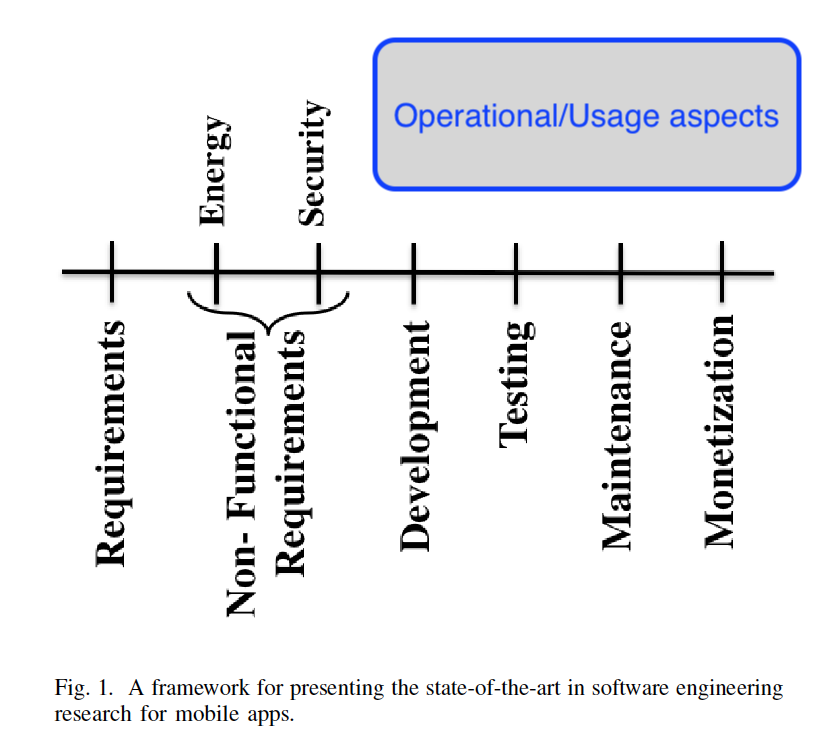
\includegraphics[width=11cm]{images/related-work/future-trends-in-sweng-for-mobile-apps-fig-1-annotated.png}
    \captionof{figure}{Annotated version of the framework for presenting the state-of-the-art in software engineering for mobile apps SANER2016~\citep{nagappan2016_future_trends_in_sw_eng_for_mobile_apps}}
    \label{fig:nagappan2016_future_trends_in_sw_eng_for_mobile_apps_figure_1_annotated}
    } % Thanks to https://tex.stackexchange.com/a/232290/88466

Mining review data for various forms of data including requests for bug fixes as is using rating as an assessment of goodness. 
Figure~\ref{fig:nagappan2016_future_trends_in_sw_eng_for_mobile_apps_figure_2_annotated} is an annotated version of their `Figure 2'. Various sources of information can be used by the development team, of these ratings and reviews are broadly researched, whereas device-level and app-level analytics have not been previously researched.

    {\centering
    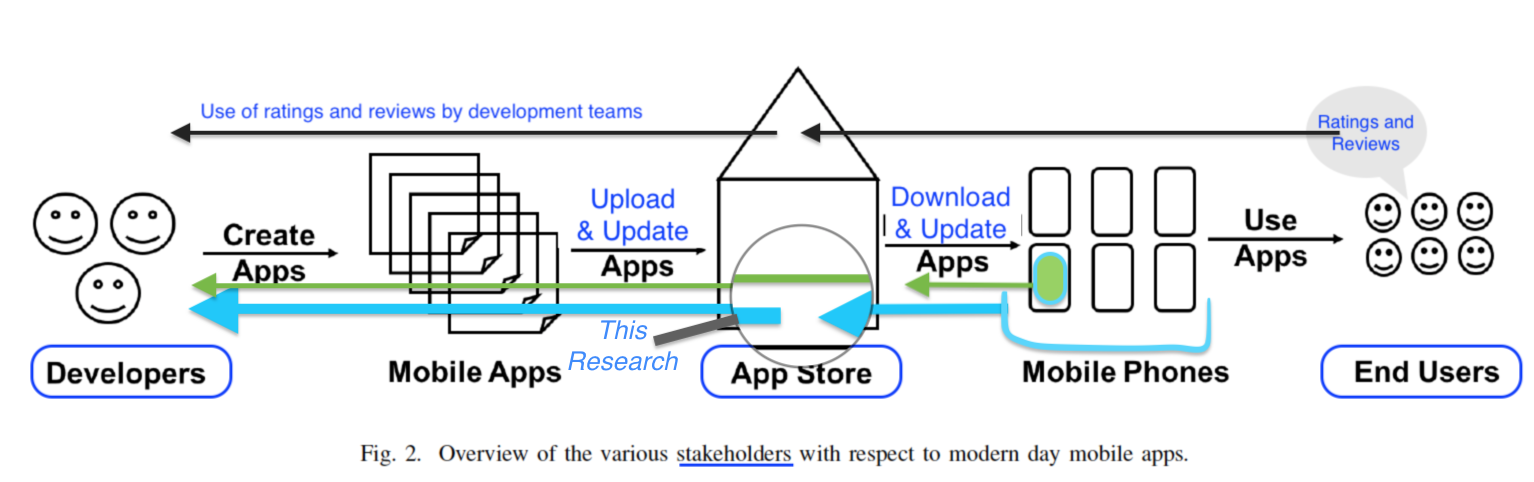
\includegraphics[width=12cm]{images/related-work/future-trends-in-sweng-for-mobile-apps-fig-2-annotated-with-highlights.png}
    \captionof{figure}{Annotated version of the various stakeholders in the modern app store ecosystemSANER2016~\citep{nagappan2016_future_trends_in_sw_eng_for_mobile_apps}}
    \label{fig:nagappan2016_future_trends_in_sw_eng_for_mobile_apps_figure_2_annotated}
    }

One of the key challenges identified is restricted access to data held by the app store, and that the only way to gather historical information is to continually mine the app store on a regular basis.

Are failure data potentially a form of requirements? (in a similar fashion to leveraging reviews in the app store to extract `requirements'). And similarly can complaints and failure data be combined to help developers prioritise issues they should consider addressing (the paper restricted the discussion to prioritising issues the developers should be \textit{testing} for).

The authors of the paper discuss limitations they experienced, perhaps without being aware that developers of Android apps have long term access to all the reviews of their apps. Details of how developers can download these and other reports, including the data structures, are available online~\citep{google_play_download_and_export_monthly_reports}. 

\emph{``Linares-Vasquez et al. [56] propose MonkeyLab, which mines recorded executions to guide the testing of Android mobile apps."} Their approach records GUI events (click events). Members of the project team (developers, testers, etc.) perform the actions, the authors claim their log collection process could scale to collecting logs from ordinary users. Key limitations include events that aren't purely dependent on the user's GUI inputs, there would also be challenges getting users to accept such an approach where the app records every input they made. Also, they generate GUI events that have x,y coordinates - absolute positioning that may have limited portability to other devices, screen rotations, and so on. Their playback also appears to require rooted devices. There are numerous other limitations described in their paper, nonetheless their work shows promise in terms of detecting and generating patterns the students did not find. It would be interesting to compare the results using accomplished software testers with experience and expertise testing similar Android apps.

Building on a point made in this paper: \emph{``the future of app quality engineering is data driven."}~\citep{maalej2016_towards_data_driven_requirements_engineering} % cite 97.

\emph{``Thus even if the app is tested on one device, there is no guarantee that it may work on another device."} - I agree. They don't provide any substance for this statement.

\emph{``The area of software maintenance is one of the most researched areas in Software Engineering. However, due to the fact that mobile apps is a young subarea within SE, the maintenance of mobile applications remains to be largely undiscovered."} - My work does investigate aspects of maintenance. 

\emph{``Syer et al. [93] compares mobile apps to larger “traditional” software systems in terms of size and time to fix defects. They find that mobile apps resemble Unix utilities, i.e., they tend to be small and developed by small groups. They also find that mobile apps tend to respond to reported defects quickly."} - Check the details of what quickly means and how the teams discovered the defects.

\emph{``Bavota et al. [16], show that the quality (in terms of change and fault-proneness) of the APIs used by Android apps negatively impacts their success, in terms of user ratings. Similarly, McDonnell et al. [65], study the stability and adoption rates for the APIs in the Android ecosystem."} - Skim read both these papers to determine their relevance.

\emph{``Another line of work examined Android-related bug reports. Bhattacharya et al. [18] study 24 mobile Android apps in order to understand the bug-fixing process. They find that mobile bug reports are of high quality, especially for security related bugs. Martie et al. [63] analyzed topics in the Android platform bugs in order to uncover the most debated topics over time. Similarly, Liu et al. [58] detected and characterized performance bugs among Android apps."} - Looks at how the bugs were fixed and compare the practices they detected with those I'm aware of. Are platform bugs that relevant? They look at performance bugs (Android Vitals also reports performance issues, Firebase Analytics has tools for performance tracking), I'm looking mainly into reliability measurements and issues.

Following on from the challenges and future directions section on maintenance research for mobile apps: do researchers focus in areas where the streetlights are rather than where the problems are? \emph{i.e.} on where they can find material to study rather than on issues that practically affect the majority of developers of apps?

\emph{``One interesting line of future research is in estimating the maintenance cost for a mobile app. Currently there are just anecdotal estimates [3]."} - Skim read this paper.

An opening gambit for my research: \emph{``Finally as mentioned in Section IX, there are several companies that collect operational data from mobile apps that have been installed on millions of devices. Most of these companies provide the app developers with the data and some rudimentary analysis on them. There is a wide variety of reliability and performance problems that can be solved by building tools and approaches that mine such operational data (past work has barely scratched the surface of such a problem by looking more at the server side of mobile applications than the client side [92])."}

Monetization is a post-release measurement, where revenues and other business-oriented metrics are applied to consider the successfulness of a mobile app. Although the paper focuses on small development teams (see the following quote as an example) in my experience many developers have measures they use in order to assess their prior work and focus their immediate future work. 
\emph{``In such apps where the development organization is small, often the developers will also have to make several engineering decisions that could affect their bottom line. Therefore software engineering researchers have examined how we can provide data to mobile app developers so that they can make these decisions in a more careful fashion."} This may be useful to support the bug triage process that developers use when determining which of the reliability bugs they choose to fix.

\emph{``Currently there are also several analytics companies (AppAnnie [1], Quettra [9], Crittercism [6] etc.) that provide valuable usage data to developers for improving their monetization strategies. They track the downloads of apps, and how the apps are being used, when users purchase things from the app etc. These companies are able to track such user data, by incorporating tracking libraries in the mobile devices. Using this information developers are able to make smarter data driven decisions with respect to making their app more successful. However, most of these recommendations are more from a marketing perspective than software engineering perspective."}
There's a lot to unpack here. Firstly although this topic discusses monetization strategies, the use of analytics can also help developers make smarter data driven decisions with respect to making their app more successful from a~\emph{software engineering} perspective. Secondly, the tracking libraries mentioned here are added to the app rather than to the device. 
\begin{itemize}
    \item AppAnnie~\citep{appannie2021}: 
    \item Crittercism: rebranded as Apteligent, which was acquired by VMWare in 2017. A few traces remain on StackOverflow and GitHub, etc. of Crittercism's analytics products of 2015. Essentially crash reporting. Some integration into enterprise systems e.g. to Splunk.
    \item Quettra: Acquired by SimilarWeb~\citep{techcrunch2015_quettra_mobile_analytics_acquired} their focus was described as a deep understanding of the users, which was then intended to help developers improve retention and also improve targeting of adverts.
\end{itemize}

\emph{``There has been some recent initial work in this direction where Bavota et al. [16] looked at the impact of using certain APIs on the ratings and Tian et al. [94] model a set of factors (like size of app, complexity of app and its UI, quality of the library code etc.) against the ratings. They were able to find that there is initial evidence that high rated apps have a certain DNA (certain value for various factors)."}

\end{mdframed}

\chapter{Methodology}~\label{chapter-methodology}
\epigraph{Is there method in the madness?}{Anon (1964--on)}
\buzzwords{Empirical Studies, Theoretical Framework, Conceptual Framework, make assumptions explicit, methodological analysis using prior publications to identify a vocabulary - SE in practice, qualitative analysis,  the 1-2-3 of research design (question - evidence - method) ...}

\begin{wrapfigure}{R}{0.7\textwidth}
  \vspace{-0.75\intextsep}
  \begin{center}
    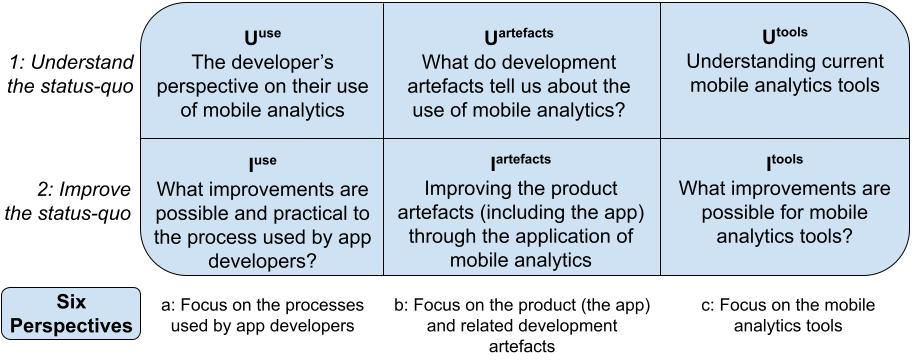
\includegraphics[width=0.66\textwidth]{images/my/six-perspectives-2x3-matrix-12-nov-2021.jpeg}
  \end{center}
    \caption{Methodology six perspectives (repeated)}
    \label{fig:six-perspectives-in-the-methodology}
\end{wrapfigure}

%In the Introduction (page~\pageref{rq-leads-to-six-perspectives}) six perspectives were introduced to support the main research question; these are repeated here in Figure~\ref{fig:six-perspectives-in-the-methodology} for ease of reference. These six perspectives consider three parallel topics: the processes, the products, and the mobile analytics tools in terms of the current practices - their use - and the scope to improve them.
%
%This research applies the 1-2-3 of research design (Question - Evidence - Method) which follow in the next three sections: 

The research needs to provide evidence to answer the main research question: \emph{How can applying analytics improve software development and software testing for mobile apps in practice?} (from Section \ref{overall-research-question}, page \pageref{overall-research-question}). The literature review has situated this question in existing research~\pending{do this once the Lit Review has been revised.}.  

To answer the research question the research needs to both understand the status-quo and to identify potential improvements, with respect to developer practices and thinking, apps and all the associated development artefacts (\textit{e.g.}, source code, issue tracking, tests, and operational configurations) that provide evidence of use, and the analytics tools themselves.

Improvements need to be compared to a baseline. In terms of this research the baseline has three perspectives: the processes currently being used by developers, the products of their development including the development artefacts and in particular the mobile app, and the mobile analytics tools themselves. Similarly it is appropriate to consider the improvements in terms of three perspectives, \textit{i.e.}: the processes, the artefacts including in particular the behaviour of the mobile app in use, and finally in terms of improvements possible in the mobile analytics tools. These are illustrated in the six perspectives introduced in the Introduction (page~\pageref{rq-leads-to-six-perspectives}) and repeated here in Figure~\ref{fig:six-perspectives-in-the-methodology} for ease of reference.

Therefore methodology needs to include techniques that can address these two key dimensions of investigation:
\begin{enumerate}
    \item a dimension that covers the different objects of analysis: the software development processes used by app developers; the software product (i.e. app) and related development artefacts; and the mobile analytics tools; 
    
    \item a temporal dimension that allows understanding of the current status and scope for improvements relating to the objects of analysis.
\end{enumerate}

%these six perspectives.  
Hence, the methodology must 
focus on practical aspects of app development, the use of mobile analytics tools by these app development teams, the quality of these tools, and the value and impact from the perspective of these teams. It also needs to determine what \emph{is} and what \emph{could be}.

\medskip

This chapter identifies the evidence requirements in \secref{methodology-evidence-requirements}\improvement{I'm aware the first letter isn't capitalised of Section. I've got an action to improve the macro.} and then, in \secref{methodology-data-sources}, presents the data sources that were used.  Then \secref{methodology-methodology-section} describes the methodology used in this research. This is followed in turn by \secref{section-introducing-the-case-studies}, which introduces two forms of case studies, those which are app-centric and those which are mobile analytics tool-centric, and the procedure used for app-centric case studies in \secref{methodology-app-centric-case-study-procedure}. The remaining sections cover the ethical aspects~\secref{methodology-ethical-considerations-section}, the threats to validity~\secref{methodology-threats-to-validity-section}, and finally a summary of this chapter in Section~\secref{methodology-summary-section}. 

\section{Evidence requirements}~\label{methodology-evidence-requirements}
Answering this research question requires rich, contextualised evidence of how developers use mobile analytics in practice.\pending{Add paragraph before this to replay findings of literature review, together with the overarching research question. If you organise your literature review as we discussed to use the three columns of the perspectives,  you could introduce the six perspectives at the end of the Lit Review. If the Lit Review takes a different direction introduce the six perspectives here.}  
Hence, the research needs to be situated in real-world industry practice and experience, drawing on real-world apps and projects for which analytics have relevance, \textit{i.e.}, that are part of an app-store ecosystem that collects analytics, and that are used by real-world users. The evidence needs to come from the developers, from their app microcosms, and from real-world mobile analytics.



% \newthought{The research needs to be situated in the real-world}
%As the real-world apps live in an app-store ecosystem, and as the main app stores collect app analytics, the research needs to be situated in apps that are available in an app store. And as the analytics are derived from usage the apps need to be used, ideally by real-world users of those apps. 

The goal of this research is to explore and understand the use and impact of analytics on mobile app development. %, rather than produce general findings that are applicable in all context.
Therefore, in order to gain an understanding of the six perspectives outlined in Figure~\ref{fig:six-perspectives-in-the-methodology}, it is necessary to investigate different examples of mobile app development practice. In this context, a comprehensive statistically representative sample of mobile apps was beyond the scope of a PhD, as determining the characteristics of sufficient representative apps and gaining access to their development contexts would be impractical. Instead, this research adopts the approach of `purposive sampling'  as described by ~\citep[pp180-182]{flick2018_an_introduction_to_qualitative_research_sixth_ed} was considered to be a more suitable approach. (Flick uses the term `purposive sampling' which is treated as a synonym of purposeful sampling in this thesis). A similar approach has been successfully applied by other researchers undertaking in-depth, qualitative explorations of software development practice, e.g., recent work on qualitative analysis of pair programming undertaken by ~\citep[p.114]{zieris2020_phd_qualitative_analysis_of_knowledge_transfer_in_pair_programming}\footnote{\emph{``Unlike for quantitative methods, statistical generalization from a sample to the population is not a goal. Instead, qualitative studies look for information-rich cases that allow to deepen the researcher’s understanding. Early in the process, each case is treated as unique and studied in great detail; cross-case analyses follow later and are based on the well-understood individual cases."}}. 

Flick presents six strategies of purposive sampling, in p.181. Of necessity the strategy used in this research is one described by Flick as convenience, however a more appropriate term for the strategy is opportunistic, since few of the case studies were convenient. As Flick notes wryly, on p.182, `the problem of access may be one of the crucial barriers' which particularly applies when seeking access to sensitive data and information about software failures for commercial mobile apps.

In terms of purposive sampling in the research I strove to use a variety of projects and apps including: commercial and volunteer led development teams, solo developer, small, medium and large development teams, industry and opensource apps, apps that include in-app mobile analytics and those that choose not to. Some of the projects that declined to participate in the research would have helped address some of the gaps in coverage of the known varieties of projects and apps.

The research explored a variety of analytics tools, as no two are identical: they offer a variety of features and capabilities, and have distinct behaviours.  Furthermore there are tools that work at the platform level and others that work at the app level; researching tools that work at both levels helps determine and distinguish their characteristics and compare their behaviours. There is only one platform-level mobile analytics tool in Google Play, the one that Google provides. In contrast there are tens of app level mobile analytics tools so there is value in researching several these app level mobile analytics tools.

The varieties of projects, apps, and mobile analytics tools, are all intended to help to uncover emergent features, capabilities, and behaviours; they also help establish ranges of examples of improvements and concerns. An additional objective is to increase the `weight of evidence' in support of particular propositions, rather than to prove them~\citep[see p.569]{seaman1999_qualitative_methods_in_esse}, which is impractical in the scope of this research.

Note: the collection of evidence depends on the source and the availability of that source in a particular study or context. It may also be constrained by technical, legal, logistical and other factors.

\section{Data sources}~\label{methodology-data-sources}
The nature of research in a sometimes messy real-world environment means access is opportunistic and often occasional. The evidence will be incomplete, yet rich, complex, and multi-faceted. For this research the data sources include:

\begin{itemize}
    \itemsep0em
    \item Development artefacts: their epicentre is the development team. They include: app binaries, app source code, tests, work schedules, documentation, bug tracking systems, \textit{etc.}, these were collected during the various case studies and complemented by public sources for additional mobile apps. 
    \item `Grey material': includes grey data and grey literature. Some were stimulated as part of the case studies, others were found during additional background research.
    \begin{itemize}
                \item Grey data includes: various discussion forums used by mobile app developers and other online contextual information, online issue tracking and related code for opensource projects beyond those that were the focus of the app-centric case studies developed in this research (e.g., open source networking libraries used by Android apps). 
                \item Grey literature includes: online materials on mobile analytics tools, articles including on medium.com and various blogs. Some were found in response to findings during particular case studies, others were found during additional background research.
    \end{itemize}
    \item Pre-study interviews: with developers and as appropriate authorised representatives of their organisation. These were used for setting up the study and understanding the development context. They were collected as part of the case studies.
    \item Mid-study communications with developers: usually email correspondence for clarification, to obtain updates, or comment on observations. These were collected as part of the case studies.
    \item Field notes: some handwritten, others recorded as text on computers. These were collected as part of the case studies and during background research.
    \item Analytics tools and associated analytics artefacts: their epicentre is the mobile analytics tool. Analytics artefacts, in particular, were a key data source; they include various outputs including screen captures, screen-scraping and parsing, results from calling APIs, and automated emails generated by analytics tools. Product documentation, online help materials, examples, and so on were also used as data sources. For open source analytics tools, the code was also used as a data source. All these data sources were collected on an ongoing basis during case studies and during additional background research.
\end{itemize}

The evidence is mainly based in real-world cases, augmented with micro-experiments where these were more appropriate. For all of these real-world cases, collection of naturally-occurring data (e.g., development artefacts, grey material) was augmented by elicitation of additional data (e.g., interviews and communications with developers) to provide clarification, breadth and insight.  Different research methods made use of these data sources, as appropriate.

In terms of the methodology, during the active case study it is vital to collect and perform ongoing analysis of mobile analytics and whatever other materials are available. Many of these are ephemeral in nature. For instance graphs generated by analytics tools may change by the minute. There is seldom a manual for the mobile analytics outputs (\textit{e.g.} the reports), furthermore many of the reports are dependent on the underlying data and/or on changes in the underlying service, Therefore the researcher often needs to iteratively learn the mobile analytics reporting in an exploratory manner\pending{Add a link to the Expo example from LocalHalo as an example}.


Third-party mobile analytics (including those provided by Google) have terms of use. These terms of use have various names, such as a policy, \textit{e.g.} for Google Play ~\citet{google_play_developer_policy_center}. These may place limitations on data collection and use of the relevant service. For the research covered in this thesis a conservative approach was used in terms of data collection to reduce the risk of consequential issues for the researcher, the project, and the stakeholders for the app. This topic and the implications are expanded on in the Discussion chapter in Section~\secref{discussion-considerations-on-the-method}, starting on page~\pageref{discussion-considerations-on-the-method}.

The choice of tools, including the humble web browser used by the researcher, affects aspects of the ease of collection of on line reports. As an example, the screenshot capability of the Mozilla Firefox browser~\footnote{Described in \url{https://screenshots.firefox.com/}} is far richer than that provided by Google Chrome at the time of writing. Many of the reports in mobile analytics tools require extensive vertical scrolling, Firefox can capture the entire contents easily, Chrome does not. 

Similarly some content is only generated on screen on demand, in response to user actions, for example through scrolling vertically (such as using `infinite scrolling'~\citep{parker2012_infinite_scrolling}) and/or paging through reports. Others are contextual and may only appear when the relevant conditions occur. For example, the release management reports in Google Play Console appear for the first 7 days of a new release. Therefore, to capture the content the researcher (or their human/automated proxy) needs to perform these actions to obtain these contents and pertinent materials saved/safeguarded to facilitate longer term analysis and provide/record evidence. Where practical, the underlying text was collected in addition to visual content; we created software called Vitals Scraper do so for Google Play Console with Android Vitals. The text could then be processed relatively easily and without needing to be re-keyed. Note: it is not always practical or useful to record ``everything"; how much is suitable is a topic for future research. 

\subsection{Mapping the data sources to the six perspectives}
The various data sources described in the previous section each contribute to the six perspectives as indicated in Table~\ref{tab:mapping-datasources-to-six-perspectives}. The table has two indications of the strength of the contribution: `\textbf{S}' indicates a strong contribution, and `\textbf{m}' indicates a medium contribution. The blank cells indicate low, or marginal, contributions rather than necessarily no contribution at all.

\begin{table}
    \small
    \setlength{\tabcolsep}{4pt} %% default is 6pt
    \setlength{\arrayrulewidth}{0.1mm}
    \centering
    \begin{tabular}{l|ccc|ccc}
      & \multicolumn{3}{c|}{\bfseries \small Understand} & \multicolumn{3}{c}{\bfseries \small Improve} \\
      \toprule
         % &\textsubscript{u}Use &\textsubscript{u}Artefacts &\textsubscript{u}Tools &\textsubscript{i}Use &\textsubscript{i}Artefacts &\textsubscript{i}Tools \\
         \multicolumn{1}{r|}{Six perspectives} &\uuse &\uartefacts &\utools &\iuse &\iartefacts &\itools \\ % Thanks to https://tex.stackexchange.com/a/33488/88466
        \hline 
        Development artefacts                       &S &S &m &m &m &m \\
        Grey Data                                   &S &m &m &  &  &  \\
        Grey Literature                             &m &m &m &m &m &m \\
        Pre-study interviews                        &S &  &m &m &m &m \\
        Mid-study communications with developers    &m &m &m &m &m &m \\
        Field notes                                 &S &m &S &S &S &S \\
        Analytics tools \& artefacts                &m &m &S &m &S &S \\
        \bottomrule
    \end{tabular}
    \caption[Mapping data source rows to the 6 perspectives columns]{Mapping research methods rows to the 6 perspectives columns \\ S = \textbf{S}trong contribution \\ m = \textbf{m}oderate contribution }
    \label{tab:mapping-datasources-to-six-perspectives}
\end{table}

Development artefacts contribute strongly to understanding of the use of mobile analytics and the artefacts themselves. They also contribute to the understanding of mobile analytics tools, for instance as they contain the usage of any API's provided by a mobile analytics tool. Through understanding the development artefacts various potential improvements emerge across the board for each of the three objects of analysis.

Grey data, \textit{e.g.} developer-centric discussions in project issues on GitHub and Q \& A on StackOverflow, mainly contribute to understanding the current state of affairs, both the immediate issues and historical issues that may or may not have been addressed or retired through changes to the mobile analytics tools and any of their associated SDKs. While they may also hint at future improvements that's seldom the focus of the developer-centric discussions. That said, occasionally external developers to a project may also suggest and/or contribute specific improvements.

Grey literature can contribute to all six perspectives moderately. It is unlikely to contribute strongly to any, partly as the material tends to be general in nature rather than specific to particular apps or projects.

Pre-study interviews mainly contribute to understanding a team's current use of mobile analytics tools. They seldom get into detail of the development artefacts, apart from various statistics that are reported by mobile analytics tools \textit{e.g.} the crash rate of the team's app(s). They often indicate areas of improvement across the board that the team could make, but not in enough detail to provide concrete improvements at this early stage in the relationship.

Mid-study communications are often focused on understanding immediate and recent events from a variety of sources (including use, changes to the artefacts, outputs from the mobile analytics). During discussions that are part of the communications scope for improvements emerge across the board.

Field notes may well be the strongest data source overall, the only area where they're limited to a moderate contribution is in terms of understanding the artefacts - generally the understanding is primarily evidenced in the development artefacts directly, so the field notes augment these rather than being the strongest source of information for \uartefacts.

Perhaps unsurprisingly, analytics tools and associated artefacts contribute most strongly to the use and improvement of the tools themselves. They also contribute strongly to improvements in the artefacts \textit{e.g.} through identifying areas in the source code that lead to a crash.


\section{Methodology}~\label{methodology-methodology-section}
The germs of the methodology include three primary complementary sources: Ball and Ormerod's `cognitive ethnography', Runeson and Höst's `guidelines for conducting and reporting case study research in software engineering', and Seaman's `Qualitative methods in empirical studies of software engineering'~\footnote{Note: this methodology was also influenced by additional research from a variety of authors in the fields of software engineering, \href{glossary-esse}{ESSE}, and a miscellany of interesting ideas from various research fields.}.

Broadly, this research starts from what Ball and Ormerod described as `cognitive ethnography'~\citep{ball2000_putting_ethnography_to_work_cognitive_ethnography}, that is, observation-based enquiry conducted \textit{in situ} to investigate ``...the interplay between people-laden contexts and expert cognition'' (p. 149). Ball and Ormerod characterise cognitive ethnography in terms of observational specificity, verifiability and purposiveness: 

\begin{quote}
  \textit{``Our own conception of cognitive ethnography is characterized by three key features. First, it relies on small-scale data collection based around representative time slices of situated activity. As such, it demonstrates observational specificity, as opposed to the intensity of a prototypical ethnography. Second, it is purposive, in that its mode of questioning focuses on issues that are informed by some intention to intervene with, or somehow affect, existing work practices ... Third, it places a strong emphasis on verifiability, in terms of validating observations across observers, data sets and methodologies.''}   ~\citep[p.152]{ball2000_putting_ethnography_to_work_cognitive_ethnography} 
\end{quote} %

Consistent with this orientation, this research sought to derive a situated understanding of analytics (in terms of the six perspectives in Figure~\ref{fig:six-perspectives-in-the-methodology}). The insights that emerged from the more ethnographically-inspired analysis of naturally-occurring data were then investigated further and tested using other approaches, namely across-case comparison, hypothesis testing (systematic manipulation in micro experiments) and action research (evaluation through interventions in specific cases) -- consistent with Ball and Ormerod's emphasis on verifiability.  

As Runeson and Höst note, software engineering motivates specialised research methodologies as the study objects: develop software, they are project oriented, and the work is advanced engineering work by highly educated people~\citep[pp. 132-133]{runeson_2008_guidelines_for_conducting_and_reporting_case_study_research_in_sw_eng}. % See below comment for the relevant text.
These criteria apply to all the case studies in this research and therefore specialised research methods were developed in order to perform the research effectively and productively. 

\begin{comment}
The study objects are 1) private corporations or units of public agencies developing software rather than public agencies or private corporations using software systems; 2) project oriented rather than line or function oriented; and 3) the studied work is advanced engineering work conducted by highly educated people rather than routine work. 
\end{comment}

My research is situated in development teams who create mobile apps and use software tools - in particular mobile analytics - in order to provide apps that work adequately for their userbases. As Seaman notes, it's important to study \emph{``nontechnical issues and the intersection between the technical and nontechnical in software engineering"}~\citep[p.557]{seaman1999_qualitative_methods_in_esse}. The author further notes the key advantage of using qualitative methods is to force the researcher \emph{``to delve into the complexity of the problem rather than abstract it away."} (p.557).

%The research resonates with the considerations and approach described by Seaman in terms of empirical studies in software engineering~\citep{seaman1999_qualitative_methods_in_esse} which provides a useful checklist and guide for the research; and by Runeson and Höst, particularly in terms of the research methodology~\citep[p.134]{runeson_2008_guidelines_for_conducting_and_reporting_case_study_research_in_sw_eng} % I needed to explain the relevance to this methodology. 


\begin{figure}
    \centering
    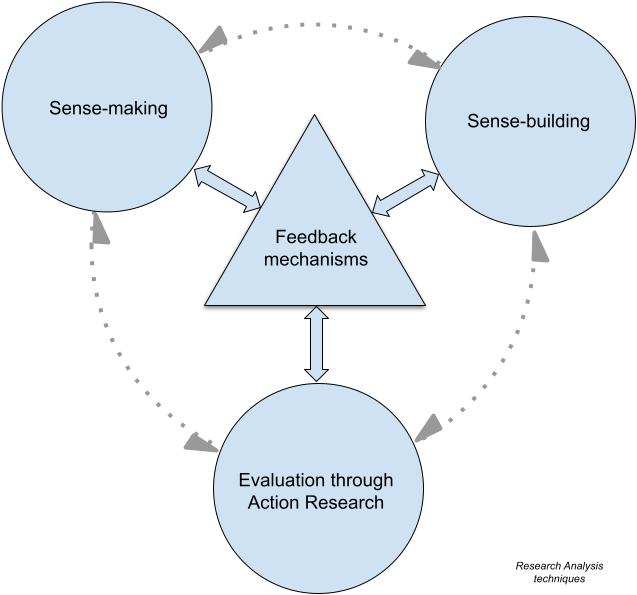
\includegraphics[width=10cm]{images/my/analysis-techniques-in-PhD-08-Nov-2021.jpeg}
    \caption{Categories of research methods}
    \label{fig:categories-of-research-methods}
\end{figure}

\subsection{Categories of research methods}
Figure~\ref{fig:categories-of-research-methods}, on page~\pageref{fig:categories-of-research-methods}, provides a visual overview of the four categories of research methods used to serve this `cognitive ethnography' approach; they include 1) sense-making, 2) sense-building, and 3) evaluation through action research. These were complemented by the fourth category 4) feedback mechanisms to help support and verify the analyses. 
%Categories of research methods (sense-making, sense-building, feedback mechanisms, and evaluation through action research). Each has a distinct purpose which will be discussed in the rest of this section. 

Note: Figure~\ref{fig:categories-of-research-methods} is an over-simplification with clear boundaries between the categories in order to convey the alignment of methods to purposes, and the categories are not discrete.  Some methods include several data sources, and some data sources are analysed using several methods. In practice, individual research methods provided multi-faceted contributions; for instance local app experiments contributed to both sense-building and sense-making. 


\medskip

%\subsection{Overview of the research methods}
%Various methods were chosen to address the research needs by engaging with data collected from actual practice, as summarised in Table ~\ref{tab:mapping-analysis-to-six-perspectives}, which groups the methods under their main category, illustrated in Figure~\ref{fig:categories-of-research-methods}, and maps them to the six perspectives. 

Table ~\ref{tab:mapping-analysis-to-six-perspectives} identifies the various research methods, groups them in terms of their roles in the research (as illustrated in Figure~\ref{fig:categories-of-research-methods}), and maps them to the six perspectives.  Each of these research methods includes data collection \textit{and} analysis unless otherwise stated.


\begin{table}
    \small
    \setlength{\tabcolsep}{4pt} %% default is 6pt
    \setlength{\arrayrulewidth}{0.1mm}
    \centering
    \begin{tabular}{l|ccc|ccc}
      & \multicolumn{3}{c|}{\bfseries \small Understand} & \multicolumn{3}{c}{\bfseries \small Improve} \\
      \toprule
         % &\textsubscript{u}Use &\textsubscript{u}Artefacts &\textsubscript{u}Tools &\textsubscript{i}Use &\textsubscript{i}Artefacts &\textsubscript{i}Tools \\
         \multicolumn{1}{r|}{Six perspectives} &\uuse &\uartefacts &\utools &\iuse &\iartefacts &\itools \\ % Thanks to https://tex.stackexchange.com/a/33488/88466
         
        \hline 
        \textbf{Sense-making} & & & & & & \\
        (comprehension and exploration) & & & & & & \\
        Beacon finding and    &Y &y &Y &y &y &y \\
        Drill Down            &y &y &Y &Y &y &y \\
        %\tabucline[1pt on 3pt]  \\ % See https://tex.stackexchange.com/a/109301/88466 however here it is terminated prematurely and a bit heavy 
        % Or try https://tex.stackexchange.com/a/229334/88466 or https://tex.stackexchange.com/a/613907/88466 if I've not collapsed these two previous rows soon.
        % Or use a newer latex package, see https://tex.stackexchange.com/a/611494/88466 

        \hline
        \textbf{Sense-building} & & & & & & \\      
        %(Integration and differentiation)    & & & & & & \\        
        (micro-experiments and macro-discoveries) & & & & & & \\
        Local App Experiments   &y &Y &Y &  &Y &Y \\
        FOSS Contributions      &  &  &Y &  &  &Y \\
        Across Case Comparisons &Y &y &Y &Y &y &y \\        
        
        \hline
        \textbf{Feedback mechanisms} & & & & & & \\
        (triangulation and validation) & & & & & & \\
        Ask The App Devs      &Y &y &y &y &y &y \\
        Ask The Tool Devs     &  &  &Y &y &y &y \\
        Grey Literature \& Grey Data Analysis       &y &y &Y &y &y &  \\
        Code Analysis         &y &Y &  &y &y &  \\
                
        \hline
        \textbf{Evaluation through action research} & & & & & & \\
        (embedded intervention)  &y &Y &y &Y &Y &y \\
        Observation and Analysis &Y &Y &Y &Y &Y &y \\
        Field Experiment         &y &  &  &Y &Y &  \\
        Hackathon                &y &y &  &Y &Y &  \\
        
        \bottomrule
    \end{tabular}
    \caption[Mapping research methods rows to the 6 perspectives columns]{Mapping research methods rows to the 6 perspectives columns \\ Y = Strong mapping \\ y = Weak mapping \\FOSS = Free and Open Source Software}
    \label{tab:mapping-analysis-to-six-perspectives}
\end{table}


`\textbf{Sense-making}' methods were concerned with understanding current practice (as reflected in artefacts, tools, and developers' practices and perspectives -- i.e., perspectives \uartefacts, \utools, and \uuse) and identifying potential improvements in tools and in how analytics are used in app development and maintenance (i.e., perspectives \itools and \iartefacts). The research methods include beacon-finding (see page~\pageref{section-beacon-finding-method}) and drill-down (see page~\pageref{drill-down-research-method}).

Sense-making incorporates an iterative pattern of \textbf{beacon finding} to identify areas of interest within a case, \textbf{drill down}\unsure{Does putting the methods in bold help with readability?} to investigate one or more beacons, and comparisons both within and across~\footnote{While across case comparisons are grouped under sense-building they also help with sense-making.} cases to identify patterns, relationships, counterfactuals~\footnote{\emph{``...relating to or expressing what has not happened or is not the case." Oxford Languages.}}, as some characteristics emerge in contrasts across and between a body of studies. 
%
Comparisons were performed iteratively on an ongoing basis (for active apps the values are not constant). These comparisons included comparisons across releases, using different windows of time, on different dates, comparisons with peers, and so on.


`\textbf{Sense-building}' methods build on insights found through sense-making. The research methods included micro-experiments, carried out on local apps (see page~\pageref{local-app-experiments-research-method}), FOSS contributions\unsure{Arosha's suggested alternative concepts of white and black box testing of the tools. I'm mulling these over. TBD.} (see page~\pageref{foss-contributions-research-methods}), and across case comparisons (see page~\pageref{across-case-comparisons-research-method}).

Local app experiments (see page~\pageref{local-app-experiments-research-method}) were used to investigate detail and give insight into the relationships between tools, quality of analytics, and potential impact of analytics use on apps (i.e., perspectives \uartefacts, \utools, \iartefacts, \itools).

Across-case comparisons (see page~\pageref{across-case-comparisons-research-method}) identify macro-discoveries -- that is, they identify characteristics and patterns that were not evident in individual case studies, potential improvements to practice (i.e., perspectives \uuse and \iuse), as well as the influence of the quality of tools in practice (\itools). They can also corroborate and/or challenge findings found in individual cases.


`\textbf{Feedback mechanisms}' were used to support and verify the other analyses, by comparing observations to other evidence, or by asking developers for clarifications or reflections. Feedback mechanisms are used throughout the research and mainly contributed to the understanding of perspectives associated with (\uuse, \uartefacts, and \utools), nonetheless they were also frequently used when considering improvements (\iuse, \iartefacts, and \itools). 

`\textbf{Evaluation through action research}' methods were largely concerned with evaluation of the effect of improvements in the use of analytics, in terms of adoption into use and app performance (i.e., perspectives \iuse and \iartefacts). It includes three research methods: 1) observation and analysis, 2) field experiment, and 3) hackathon. These are explained in page \pageref{section-evaluation-through-action-research-method} onwards. 

The research was iterative, moving through sensemaking, sensebuilding and feedback mechanisms repeatedly as new cases are studied or new insights emerge.  The methods and the data sources often also inform several of the six perspectives.  The research methods are introduced in more detail in the sections that follow.

\subsection{Sensemaking}
% c.f. https://en.wikipedia.org/wiki/Sensemaking_(information_science)
%1) Identifying patterns (inductive analysis) c.f. grounded theory. 2) 

`Sensemaking' includes 1) beacon finding and 2) drill down. These were used for \textit{inductive analysis} of artefacts, broadly consistent with grounded theory where the statements or propositions are supported in many ways by the data discovered in development and analytics artefacts; \textit{c.f.} the discussion of `grounded theory' methods where the propositions are ``grounded" in the data~\citep[p.566]{seaman1999_qualitative_methods_in_esse}~\footnote{This research in turn cites:  Glaser, Barney G., Anselm L. Strauss, and Elizabeth Strutzel. \emph{"The discovery of grounded theory; strategies for qualitative research."} Nursing research 17, no. 4 (1968): 364., which I have not been able to access.}\pending{Marian to help with the grounded theory aspects e.g. via~\citep{zieris2020_phd_qualitative_analysis_of_knowledge_transfer_in_pair_programming}}. 

\julian{\textit{c.f.} `Cognition in the wild', as a comparison with grounded theory. Cognition in the wild provides a parallel example of rich and emergent findings from the real world that would be very hard to specify or determine the factors that applied at the time the ship was being brought under control~\citep{hutchins1995_cognition_in_the_wild}.}\pending{I'm waiting to borrow Marian's copy of this book, then I can write about the connection to this research and the methodology.}

These sense-making methods were amplified through the feedback mechanisms, covered shortly. 
%In addition a third method, local app experiments, was used to create conditions for additional sensemaking.

\begin{figure}
    \centering
    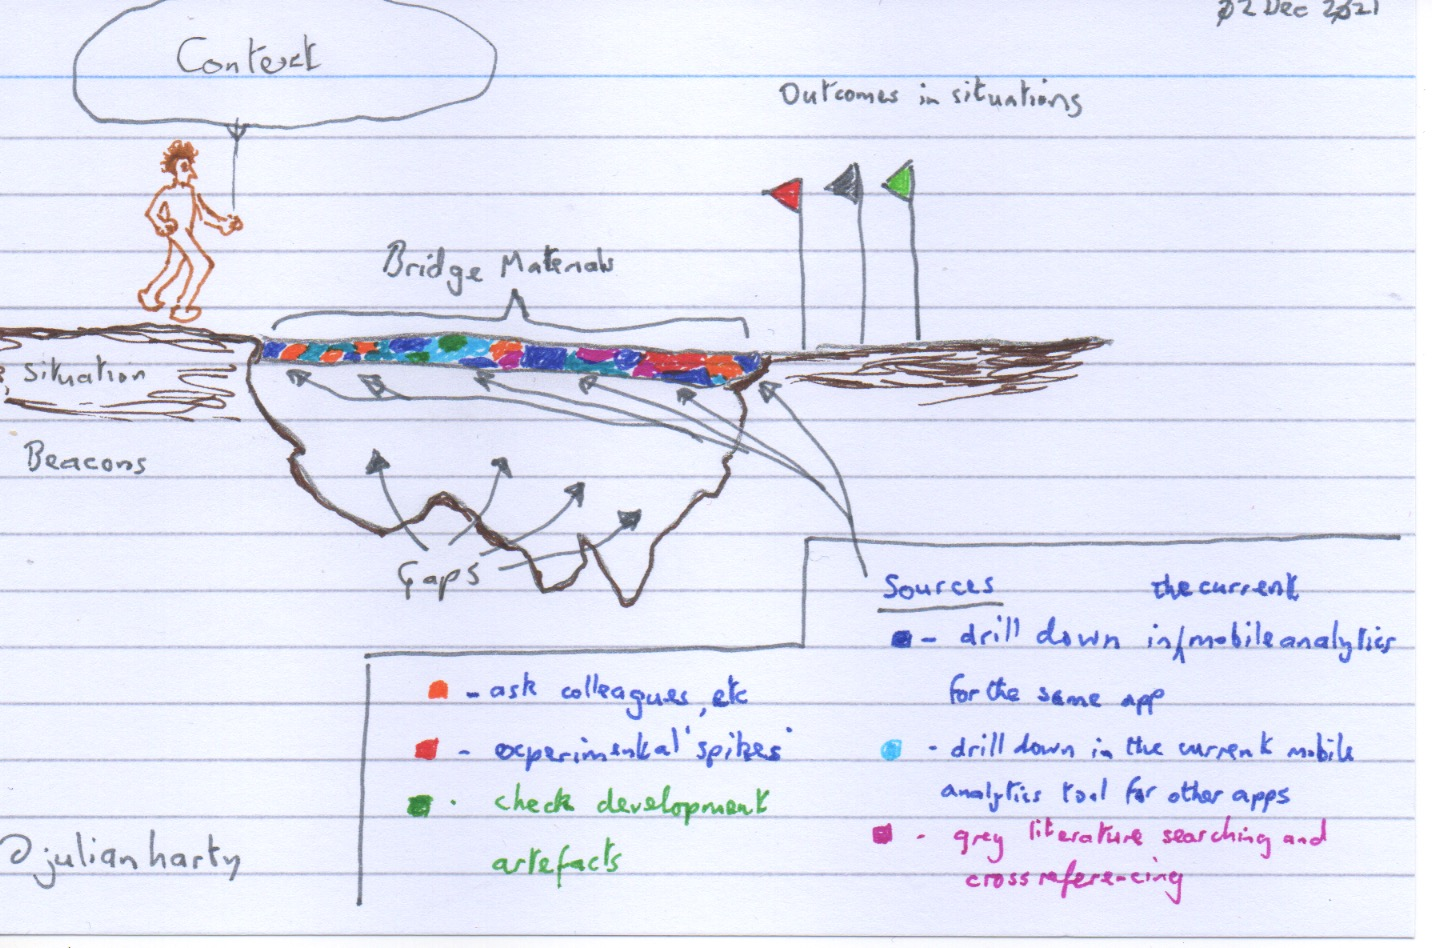
\includegraphics[width=15cm]{images/rough-sketches/the-sense-making-metafor-revised.jpeg}
    \caption{Custom Sense-Making Metaphor diagram}
    \label{fig:the-sense-making-metafor-revised}
\end{figure}

Sense-making has been used in research in Information Science, the topic is well summarised in \citealt{naumer2008_sense_making} co-authored by Karen E. Fisher, and by Brenda Dervin who created the sense-making methodology presented in this paper. Figure~\ref{fig:the-sense-making-metafor-revised} presents a revised edition of the Sense-Making Metaphor in Brenda Dervin's methodology adapted here to illustrate sense-making in this research. It broadens the approach to indicate the range of potential sources used in sense-making for mobile analytics, here illustrated with individual colours~\footnote{The choice and selection of colours illustrative and not intended to be definitive.}. The range of sources include:

\begin{itemize}
\itemsep0em
    \item Drill-down in the current mobile analytics tool for the same app.
    \item Drill-down in the current mobile tool for other apps. (If the app incorporates other mobile analytics tools these tools may also help where there is overlapping content common to both tools; for example crashes reported in both Android Vitals and in Crashlytics.)
    \item Comparing various analytics artefacts, particularly reports, using various criteria.
    \item Searching grey data and grey literature and cross referencing of materials.
    \item Asking people: for instance colleagues, the developers of the app, the developers of the mobile analytics tool, \textit{etc}.
    \item Experimental `spikes' (these tend to require significant effort so are not likely to be used lightly).
    \item Check development artefacts as these may provide relevant and pertinent information and clues.
\end{itemize}

In short, beacons need to be understood in context and the context includes seeking and obtaining additional information from a wide variety of sources. That said, of the many potential sources, two are core to sense-making: beacons are first found and thereby they also become a source and then drill-down used to make sense of the information pertaining to the beacon. The others are also useful, however for the purposes of this research they mainly serve another category and are therefore allocated to that category.

%Further reading: two of Brenda Dervin's figures for her sense-making metaphor are adapted very slightly if at all in https://asistdl.onlinelibrary.wiley.com/doi/epdf/10.1002/asi.20400 which focuses on gap-building~\citep{savolainen2006_information_use_as_gap_bridging_the_viewpoint_of_sensemaking_methodology}.

%Sensemaking has been applied to various aspects of computing and software development, for example: in program comprehension, in understanding end-users' understanding of spreadsheets~\citep{grigoreanu2012_end_user_debugging_strategies_a_sensemaking_perspective}. COULD-DO discuss the work of~\citep{naumer2008_sense_making}. Our use of sensemaking is inspired by sensemaking in research into these areas. 

%The following methods primarily helped with sense-making: analysing and ``making sense" of mobile analytics tools, development artefacts, and the developers' perspectives on their use of mobile analytics. 

\subsubsection{Beacon-finding}~\label{section-beacon-finding-method} %concept, adaption to suit this research, examples.

The notion of \textbf{`beacons'} is borrowed from research on program comprehension; for instance by Wiedenbeck, who helped establish the notion of beacons in software development: ~\emph{``In programming, beacons are lines of code which serve as typical indicators of a particular structure or operation"}~\citep[p.679]{WIEDENBECK1986_beacons_in_computer_program_comprehension}. The work was extended and updated to explicitly consider the effects of beacons in comprehension of source code, for instance in~\citealt{crosby2002_roles_beacons_play_in_comprehension_etc}.

The notion of beacons was generalised for this research to include indicators in the analytics of something of interest, or something that required attention.  And so 'beacon finding' was an inductive process by which significant indicators in the analytics data were used to identify areas of the code base that required further investigation.  Mobile analytics may include source code that calls APIs in the application's source code, however the bulk of the contents that need to be comprehended comes as outputs from the mobile analytics tools, therefore the beacons will differ accordingly. In this research the beacons include: the shape of graphs in mobile analytics report, failure clusters, a method call in stack traces, and so on\pending{I'm assembling some relevant raw notes in a new file: beacons-in-mobile-analytics.tex TBD where and how I'll integrate it.}.

%\marian{Now specify how you spotted beacons... I looked for things on this basis, how I kept track of things, what selection criteria were used and why?}

Beacons emerge in various ways. For instance in reports they include: anomalies within a report, mismatches and inconsistencies between two sibling reports or between a master report and the linked detailed report~\pending{Arosha, suggested introducing these terms for different types of report when discussing analytics tools in the lit. review. I agree, TBD once the lit. review has been reworked.}, in the shape of the curve of a graph, in the distribution and groupings of aggregate data, and so on. Similarly, alerts as determined by a mobile analytics service may be considered potential beacons being `promoted' by the mobile analytics reports. 

The most common method of recording potential beacons was using web browser screenshots and/or other mechanisms that preserved information electronically. Some were annotated as part of the beacon-finding and drill-down analysis. Additional notes were written both electronically and/or in physical notebooks. 

Selection criteria included: top ranking results, atypical rates of change, adverse changes to reliability, novel failures particularly for the most recent release, etc. A consistent and overriding criterion was to seek beacons that indicated flaws and failures that could materially and adversely affect the user experience of the app for one or more users of the app.


%\textbf{Beacon finding} seeks potentially relevant indicators, typically within bounded domain such as software code. Beacons help to convey meaning and are used for comprehension, for instance by programmers who wish to understand source code~\citep[page i]{crosby2002_roles_beacons_play_in_comprehension_etc}. The concept of beacons in source code has been studied by various authors for several decades; for instance by Wiedenbeck, who helped establish beacons in software development: ~\emph{``In programming, beacons are lines of code which serve as typical indicators of a particular structure or operation"}~\citep[p.679]{WIEDENBECK1986_beacons_in_computer_program_comprehension}. The work was extended and updated to explicitly consider the effects of beacons in comprehension of source code, for instance in~\citealt{crosby2002_roles_beacons_play_in_comprehension_etc}.
 


% I'm not sure where to discuss beacons in conversations: for instance in a developer's description of their use of mobile analytics to assess the quality of the app - they exist to me - TBD.


\subsubsection{Drill-down}~\label{drill-down-research-method}
Beacons stimulate interest, the interest needs to be satisfied one way or another by investigating the beacons and their underlying information sources. 
Are the identified beacons genuinely significant? What do they signify or relate to in the app and its usage, etc.?  Drill-down starts with the original data sources, but may draw in other data sources for example to clarify relationships, responses by the developers, etc.

Here are 2 examples:  % Temporarily these are a list, they'll probably be embedded in the paragraph once the relevant examples have been incorporated. The pending command links were poorly formatted when the text was inline.
\begin{enumerate}
    \itemsep0em
    \item 1) investigating a large spike in the overall crash rate to determine the constituent causes \pending{Add link to an actual example in a case study}
    \item 2) understanding a Java WebView Exception \pending{Again provide a link to the example in my thesis)}.
\end{enumerate}

Note: it transpires developers use a similar form of sense-making, this is discussed in \secref{sensemaking-and-decision-taking-by-developers-section}, starting on page \pageref{sensemaking-and-decision-taking-by-developers-section}.

\clearpage
\subsection{Testing mobile analytics tools on a continuum}~\label{section-testing-mobile-analytics-tools-on-a-continuum}

\buzzwords{Translucence, various levels of opacity, white+grey+white box testing}

 The research includes three methods of testing in order to evaluate aspects of the mobile analytics tools.\improvement{FYI this subsection is a w-i-p to explore whether the following material is clearer and more faithful to the research than the current local app experiments and FOSS contributions. If it is, this section will be woven into the rest of the methodology chapter. The catalyst was a suggestion by Arosha on \nth{8} Dec 2021.} 
 They are all forms of micro-experiment. The methods of testing are loosely based on familiar concepts of black-box, white-box, and grey-box testing where there are various levels, or depths, of opacity in the system under test.

The tests include: testing the developer support channels, testing the process and experience of providing contributions to several opensource projects owned by mobile analytics tool providers, and testing mobile analytics tools by treating them as a black-box system under test (SUT) though the development of several small-scale Android apps. These small-scale apps were used to exercise the app store's pre-launch facilities and several of the in-app mobile analytics tools.\pending{This needs connecting to the material that follows.} 

Add a table: mapping the methods to the granularity, show the connection to the colour of box and how they connect to the object of the testing.\pending{Add a table showing the mapping}


\newthought{Developer support channels}


\newthought{Mini, local app experiments} 
Essentially the same story as it the local app experiments method.

\newthought{Testing contribution processes} 
Code contributions to opensource packages of commercial mobile analytics projects.
%
Essentially the same material as in the FOSS contributions method. The hypothesis was that some companies make their proprietary code available as opensource but do not actually accept contributions. The experiments involved creating small improvements to one or two aspects of their opensource projects and then creating pull requests to discover their acceptance process and what the results would be in terms of them accepting the pull requests.

\newthought{Working with the Iteratively product}
This experiment emerged from earlier collaborations with the founders of Iteratively. They offered free access to their product. The experiment incorporated their product into a small Android app where the analytics was routed by their SDK to Amplitude. The experiment provided a translucent view into their SDK and its behaviour in terms of the integration with Amplitude and also the support for custom implementations.

\newthought{Collaboration with Google is also a form of testing}
In some ways the collaboration with Google's engineering team was a form of testing to see whether they would firstly accept the contributions as valid and of merit, and then whether they would improve their product to address flaws reported to them during the collaboration. Google... TBC.

%%%%%%%%%%%%%%%%%% See also %%%%%%%%%%%%%%%%%%%%%%
% https://en.wikipedia.org/wiki/Transparency_meter
% https://en.wikipedia.org/wiki/Opacity_(optics)
\clearpage

\subsection{Sense-building}
Sense-building moves beyond sense-making. Sense-making aims to understand \textit{what is} while sense-building involves direct action and more active research, for instance: to devise and run experiments to learn more about the behaviours of mobile analytics, and to seek patterns and generalisations across tools, and case studies. Two methods were used primarily in sense-building: local app experiments and across-case comparisons, together with a third method: \href{glossary-FOSS}{FOSS} contributions. 

\subsubsection{Local-app experiments}~\label{local-app-experiments-research-method} 
\textbf{Local app experiments} were used to \textit{test the understanding} of the relationships between the usage and the analytics through manipulations of apps and observation of the effects -- hence, the local app experiments were used to test some of the patterns identified in the inductive analysis. They consist of \textit{micro-experiments} involved creating and developing small mobile apps intended to exercise particular aspects of mobile analytics~\footnote{Similar to the `invent the future' adage, for example: \url{https://quoteinvestigator.com/2012/09/27/invent-the-future/}}). The inputs to an app were directed in order to determine the outputs from mobile analytics. These helped to answer questions and gaps observed as part of sensemaking.  The local app experiments gave insight into the relationships between tools, quality of analytics, and potential impact of analytics use on apps (i.e., perspectives \uartefacts, \utools, \iartefacts, \itools). 

The apps that were developed as local-app experiments are small mobile apps and not intended for production use. They were developed in order to investigate the relationships between the inputs (such as usage) and the analytics outputs (such as reports) through deliberate manipulation of the inputs and observation of the consequences.  

The local-app experiments allow for tighter control on the usage, \textit{i.e.} the inputs, in comparison to the unfettered use of real-world mobile apps. They can help surface behaviours and provide for tighter evaluation in the early, pre-launch/pre-production phases. %I can't say feedback as that'd conflate the other use of feedback here in the methodology.
The local app experiments were used to test some of the patterns identified in the inductive `sensemaking' analysis.

Where practical the source code of these apps is made available under a permissive opensource license to facilitate further research by others and in order to facilitate inspection by and feedback from others.

%\akb{Also explain how the results of these experiments connected to other parts of the method? e.g., did they change / add to the sense-making activities?}
The results of the local app experiments helped augment the across-case experiments, particularly in terms of providing additional results to compare with those from the app case studies. They also informed discussions with the app and tool developers. 

\subsubsection{FOSS contributions}~\label{foss-contributions-research-methods}
\href{glossary-FOSS}{FOSS} contributions provided experimental evidence where contributions were offered to public repositories of opensource mobile analytics components to explore their willingness to accept contributions and their process for doing so. The contributions were each intended to improve one or more elements of the respective codebase and thereby improve the respective product offering. They were small in size and made on an \emph{ad-hoc} basis rather than systematic~\footnote{While systematic contributions may be a valid approach to research this topic, it was not core to this research.}.


\subsubsection{Across-case comparisons}~\label{across-case-comparisons-research-method}
\textit{Across-case comparisons} were concerned largely with understanding current practice and identifying potential improvements to practice (i.e., perspectives \uuse and \iuse), as well as the influence of the quality of tools in practice (\itools). This method draws on the approach discussed in \citet[pp. 567-569]{seaman1999_qualitative_methods_in_esse}, \textit{e.g.} to compare pairs of case studies to determine variations and similarities, with the additional considerations of seeking areas of potential improvements based on findings from the various case studies.

Similar to using various software testing techniques to find bugs, making comparisons across the case studies can help to identify more of the behaviours of mobile analytics, their use, and their efficacy. Across-case comparisons can increase the probability of seeing fresh characteristics and establish similarities across cases. The comparisons across case studies help establish norms (which can also be used to identify beacons, and anomalies), patterns (and anti-patterns), variety, and ranges. 

Comparisons across cases (\textit{i.e.} across projects and their mobile apps) helps both researchers and developers, albeit their interests and focus may differ.

\begin{itemize}
    \item \textbf{For developers}: they can compare the reports for their apps with the results others obtain. Doing so may help them identify problems-in-common (shared problems) and fixes-in-common that work for many apps with similar failures. They can also establish norms and the comparisons help provide triangulation and perspective. Some developers also find peer-group comparisons stimulating.
    
    \item \textbf{For researchers}: across case comparisons include `plus one'~\citep[pp 28-29]{aurini2016_how_to_of_qualitative_research} research that can help uncover emergent behaviour, reinforce existing findings, and so on. The across case comparisons also provide additional microcosms where new findings are discovered in the behaviours of apps, the tools, the development practices, and the efficacy of the use of mobile analytics performed by a wider variety of development teams.
\end{itemize}


The data and the system state for individual apps can help to increase the `coverage criteria' for a mobile analytics tool (which may be considered a system or simply a `box' as in black-box, grey-box, or white-box system)~\pending{In the planned Tools chapter I can discuss this property of the various Mobile Analytics tools.}. 

We know from a related domain, software testing, that more test cases can increase the detection rate of behaviours. For example, a paper by Briand~\citet{briand2007_a_critical_analysis_of_empirical_research_in_software_testing} discusses concepts including the concept of a cost-effectiveness curve and of what the author terms `random variations' and the effect these random variations have on fault detection effectiveness in page 5 of their paper. The set of inputs (\textit{e.g.} crash reports) into mobile analytics tool may result in various beacons - and related data - appearing in the outputs. By increasing the sets of inputs, particularly from dissimilar apps, there is the potential to increase the appearance of more beacons. And the larger volume of beacons across the projects allows for weightier analysis.

A key observation is that detection is not static nor a one-off value; behaviours come and go, particularly in mobile analytics tools where reports are often ephemeral. The value of across-case comparisons increases when the sampling increases to record more of the ephemeral behaviours and outputs.

The nature of this PhD research based on a relatively small number of apps and associated case studies means it is premature to attempt to systematically plot the number of cases against the behaviours that were observed. Instead the focus is on monitoring 
new insights vs. resonance, and how often a new case highlights something that was not noticed in previous ones, even though they were there~\footnote{\textit{c.f.} Testing and Noticing~\citep{bolton2009_testing_and_noticing} which discusses noticing (and not noticing) from a software testing perspective.}.

We also need to consider: does anything generalise beyond a single case?   


\subsection{Feedback mechanisms}
Sense-making and sense-building methods are centred on the research and driven by the researcher's focus and perspective. Unaided - even if they're productive - they risk being marginalised and disconnected from the work of others, in particular the work of those who actually develop the apps and the tools. Feedback triangulates and validates the outputs of sense-making and sense-building. 

Feedback mechanisms also corroborate and challenge the research findings; for example to calibrate particular findings with the developers who can be asked if they recognise and agree with particular findings.

In this research, four methods were used to obtain feedback, two involved asking humans and the other two interrogated existing materials created (mainly) by humans.

\phantomsection
\label{method-vectored-questions}
%A method termed `\textbf{vectored analysis}' was used with both app developers and and analytics tool developers, \textit{i.e.} during two of the feedback methods: 1) ask the app devs, and 2) ask the tool devs. 
Vectored observations/questioning/analysis was used with the aim of increasing the understanding of their work pertaining to mobile analytics. Vectored questions are purposeful and focused, they are similar to Petre's `targeted observation'~\citep[p.234]{petre2009_insights_from_expert_software_design_practice} and situated in the actual practice of the developers - their real world microcosm. They draw on multiple data sources which allows for comparison/triangulation/colligation and allows for multiple methods to gather and analyse data -- all with a focus on the research questions.\pending{Marian will rewrite this paragraph.}


\subsubsection{Ask the app devs}~\label{section-ask-the-app-devs-research-method}
The developers of the apps are uniquely able to voice their perceptions and thinking on their use, experience, and perceptions of using mobile analytics. They are therefore well placed to provide feedback on their use of mobile analytics and also answer questions about their use of mobile analytics in their development artefacts and their perceptions of the mobile analytics tools.

They are also busy with their challenges related to developing and improving the mobile apps they are responsible for. As Petre notes in~\citep{petre2009_insights_from_expert_software_design_practice} experts are willing to try/explore many tools however they focus on what can help them, and they may discount many aspects of the mobile analytics tools including some of the characteristics and behaviours of interest from a research perspective. Nonetheless from a research perspective it may be useful to learn more about why they have discounted or rejected various aspects of the tools. 

\subsubsection{Ask the tool devs}~\label{section-ask-the-tool-devs-research-method} 
%  &  &  &Y &y &y &y \\
The tool developers understand their mobile analytics tools in depth and many have a unique vantage point to observe how their mobile analytics behaves across a large population of apps. Furthermore they are well placed to design, implement, and release fixes and improvements to their mobile analytics products and services. They understand the rationale of their mobile analytics tools and their user-base. And yet, they do not know everything about how their tools are used or perceived and many are keen to receive feedback and insights accordingly.

The research method entails communicating with knowledgeable, available and interested people who develop (in the broad sense) the relevant mobile analytics tool. The communication may be direct or indirect (for instance via their customer service, via online feedback links, or in the form of contributions to their opensource project). Being able to provide succinct, clear, timely, and relevant communications may increase the chances of engaging in a mutually productive dialogue.

\subsubsection{Grey literature and grey data analysis}~\label{section-grey-literature-and-data-analysis-research-method}\improvement{So two shades of grey? :)}   
%   &y &y &Y &y &y &  \\
A great deal of grey literature, and grey data~\citep[pp 219-221]{banks2010_blog_posts_and_tweets_the_next_frontier_for_grey_literature}, is available online, covering mobile analytics and to errors, problems related to source code and libraries used in real-world mobile apps. The main sources of relevant grey data include Stack Exchange websites frequented by mobile app developers (particularly \href{https://stackoverflow.com/}{stackoverflow.com}) and GitHub. 

Both Stack Exchange and GitHub provide comprehensive and useful search capabilities which help find relevant content, for instances examples where other development teams have found, understood, and addressed particular crashes in their Android app that also apply to the app in the case study.

\href{https://stackoverflow.com/}{stackoverflow.com} provides facilities that encourage meta-data to be provided by users of the site \textit{e.g.} tags, votes, accepted answer flag, \textit{etc.} and their search provides facilities to perform searches that use meta-data as well as free text~\citep{stackoverflow2021_search_help}.

The nature of GitHub projects provides some inherent structure which can be utilised when performing searches, for example to search issues and pull requests~\footnote{\url{https://docs.github.com/en/search-github/searching-on-github/searching-issues-and-pull-requests}}. Note: GitHub uses the term `qualifier' in the online documentation~\citep{github2021_searching_code_github_docs}, and the terms `prefix' and `tag' in their online search page \url{https://github.com/search} to describe their mechanisms to filter the search results. These mechanisms facilitate structured searches of public projects (and those the individual also has access to).

% Crashlytics search should be mainly matched in Android projects because of the target filename. https://github.com/search?q=crashlytics+filename%3Abuild.gradle&ref=simplesearch 

% If I ever have the time and purpose, continue trying to use https://sourcegraph.com/search in case it's able to perform the searches we did in our joint research. Ditto try again with github's v4 search API.

There are similarities in searching programmer-generated grey literature and the low-ceremony evidence described in \citet{scaffidi2007_toawards_a_calculus_of_confidence, scaffidi2007developing} where the sources of evidence include votes received by questions and answers on StackExchange sites and on public issue tracking sites including GitHub and Google. % ADD example of Google  

\subsubsection{Code Analysis}~\label{section-code-analysis-research-method}   
%       &y &Y &  &y &y & \\
Source code provides a snapshot of raw ingredients which is used by the development team's build process in order to generate an app. The source code often includes at least one build `recipe'~\footnote{For most Android apps the main build recipe is in the file \texttt{./app/build.gradle}.} so the build can also be evaluated and hopefully reproduced~\footnote{Aside from sensitive ingredients such as signing keys used to digitally sign each binary when it is created.}. The source code's repository augments the source code by recording the historical evolution of the source code.

Code analysis in the context of mobile analytics involves searching for indications of the use of one or more in-app mobile analytics libraries in the project's source code~\footnote{The Exodus Project \url{https://reports.exodus-privacy.eu.org/en/} is one of several tools that can identify the mobile analytics library in an application's binary file.}. The steps performed to identify indicators %c.f. beacons as used in this chapter
of the use of a mobile analytics library include:

\begin{enumerate}
    \itemsep 0em
    \item Details in one or more \texttt{gradle} scripts where the analytics is added as a `dependency', the version of the dependency provides useful meta-data on whether the analytics are actively maintained by the developers. % COULD-DO\textit{e.g.} add code snippet e.g. see https://firebase.google.com/docs/analytics/get-started?platform=android#add-sdk
    \item Initialisation of the analytics library in the source code, often this occurs in the Android app's \texttt{Application} class. % Ditto there's an example code snippet at https://firebase.google.com/docs/analytics/get-started?platform=android#add-sdk
    \item \texttt{Import} statements in individual source code files that reference the analytics Java package(s).
    \item Searching for one or more \textit{wrapper} class files. If these exist then extend the search for these custom classes in step 3 and 5.
    \item Search for calls to the original and any wrapper mobile analytics API classes. % e.g. based on examples including https://firebase.google.com/docs/analytics/get-started?platform=android#start_logging_events
\end{enumerate}

After the five steps have been completed the matching lines of source code are then available for analysis. 
%
The analysis can be performed for any snapshot of a codebase \textit{i.e.,} for any commit made to the version control repository. Commands such as \texttt{git blame} provide information of the particular commit where lines of code were last updated and complement analysis of the snapshots.

The application of five steps can be scripted. As an example, in joint research~\citep{harty2021_logging_practices_arxiv} a mix of manual and scripted steps were applied to enable the analysis of the use of Firebase mobile analytics in all the commits made to 57 opensource Android apps.

A useful confirmatory test to help establish the integrity of an app's codebase is to build the app using the build scripts. There may be additional documentation of the build process available \textit{e.g.} in a README file incorporated into the code base.

\subsection{Evaluation through action research}~\label{section-evaluation-through-action-research-method}
The article by ~\citet*{avison1999_action_research} on action research explains the utility and importance of Action Research in order to establish the relevance of academic research by trying out theories with practitioners in real situations and in real organisations. They recommend action research \emph{``because this particular qualitative research method is unique in the way it associates research and practice, so research informs practice and practice informs research synergistically."}~\citep[p.94]{avison1999_action_research}. Action research is particularly relevant for the evaluation where it \emph{``encourages researchers to experiment through intervention and reflect on their intervention and the implication of their theories."}~\citep[p.95]{avison1999_action_research}. 

This research applies their recommendation where the research informs the practice of both app developers and the work of the developers of mobile analytics tools. Conversely, the research is enriched through understanding the practices and the potential for the application of mobile analytics to help improve the quality of the work of the app developers. The predominant approach to the research is through case studies. These case studies include examples where the researcher's mode of engagement was as:
\begin{enumerate}
    \itemsep0em
    \item a consultant and/or an embedded developer: an active participant integrated into the project team,
    \item a coach: of existing teams of app developers who applied the concepts,
    \item an interviewer: of various development teams to learn of their practices and results,
    \item an analyst/observer: performing static analysis of opensource code repositories~\footnote{Analysis of proprietary code repositories is also possible, but not practicable for this research owing to confidentiality agreements.}.
\end{enumerate}

All these modes of engagement include at least some observation and analysis. 

The coach role and embedded developer modes ended up being fairly similar. They both included organising a hackathon for the respective project and a field experiment for the respective project. The material differences were two-fold: a) the embedded developer role was for many months, whereas the coach role was for several months, also, b) the embedded developer role included contributions to the project's code-base. 

The consultant role included engineering leadership, mentoring developers and product owners in learning how they could integrate mobile analytics into their work practices, co-writing automated tests and related code, code reviews, and working with various mobile analytics tools throughout the assignment.

Note: this research predates the publication of a detailed article on `The ethics of action research participation'~\citep{davison2021_the_ethics_of_action_research_participation} that includes six principles for `Integrated Action Research'. These would be of interest in future related work.

\subsubsection{Observation}~\label{section-observation-research-method}
In this research observation includes observations of either or both development artefacts and analytics artefacts. One example is to observe the outputs from mobile analytics tools (the analytics artefacts) and what the developers do with these subsequently. 

\subsubsection{Analysis}~\label{section-analysis-research-method}
In this research this method is combined with observation where the researcher provides analysis of the observations and findings to the project and development team. There are two main objectives: 1) to provide value for the project team who were willing to contribute their time and who provided access to their analytics and other artefacts, and 2) to encourage scrutiny and validation of the findings and observations.

\subsubsection{Field experiment}~\label{section-field-experiment-method}
In this research, field experiments use real-world apps and their core code repositories. They were not as rigorous as controlled experiments owing to the nature of the development teams and their priorities. Nonetheless they included a control app and an experiment app where experiments are performed on the experiment app and mobile analytics results compared for both these apps. They are also ecologically valid, ~\citep[p.126]{Ko2015_a_practical_guide_to_controlled_experiments_of_sw_eng_tools_with_human_participants}, as they are situated in real world challenges found in their core mobile apps.

The approach described in~\citep{Ko2015_a_practical_guide_to_controlled_experiments_of_sw_eng_tools_with_human_participants}: were not suitable for several reasons~\footnote{This form of research may be useful and also viable for large, funded research groups and/or for organisations such as the larger mobile analytics tool providers, particularly Google. That said, Google in particular has access to such a vast range of data about the use of their mobile analytics tools they may not need or want to perform controlled experiments of the form discussed in this research.}. 
%
My research didn't have the opportunity to compare two tools quantitatively, nor was it practical to perform quantitative research experiments as none of the projects were interested in the complexity and demands of the type of controlled experiments illustrated in their research. Therefore, the field experiments were designed to suit the specific opportunities provided by the respective projects as follows:
\begin{itemize}
    \item Hackathons were used to initiate the field experiments for the opensource projects. These were attractive to the development teams, partly as they were for a distinct period where the team were able to meet and enjoy the experience of collaborating.
    \item Both the opensource projects had multiple apps, including one that had the worst reliability of their apps (as measured by mobile analytics). The project leads saw value in helping arrange and support the hackathons. They also had apps which were suitable to act as the control for their hackathon. 
\end{itemize}

\subsubsection{Hackathon}~\label{section-hackathon-research-method}
The hackathon research method in this research applies the concepts of software development hackathons. The vital distinction is the additional concept of using mobile analytics tools as a source of information related to issues in the behaviour of one of more mobile apps supported by participants in the hackathon.

In other words, these hackathons are: \textit{a software development hackathon + use of failure data reported by mobile analytics for that team's mobile app}.

The hackathons were communal+contributive+catalytic, see: \emph{``communal (towards  community  nurturing), contributive  (issue-oriented),  or  catalytic  (towards  the search  for  innovation)."}~\citep[p.3]{medina2020_what_do_we_know_about_hackathons_etc_a_SLR} Note: The source of these terms appears to be in `A Typology of Hackathon Events'~\citep[pp. 1-3]{drouhard2016_typology_of_hackathon_events} %a paper published via \url{https://hackathon-workshop.github.io/}, 
% The 2nd workshop is no longer online, instead see https://web.archive.org/web/20181203070803/http://hackathon-workshop-2018.com/ 
They were \emph{communal} as the participants were part of common development communities (as developers for the opensource apps they contributed to); \emph{contributive} as there were common concerns about the issues the hackathons were intended to address with a strong desire for impact, ~\citep[see p.2]{drouhard2016_typology_of_hackathon_events}; and \emph{catalytic} as one of the aims was to demonstrate a new approach to the use of a dataset (mobile analytics reports) and technology (mobile analytics tools)~\citep[see p.3]{drouhard2016_typology_of_hackathon_events}.

No rewards were offered to participants beyond being at the respective hackathon and participating. These are termed `Single-Application' hackathons in~\citealt[p.5]{briscoe2014_digital_innovation_the_hackathon_phenomenon}. The participants were current members of the respective development team.

In the context of this research the hackathons included the researcher and a highly experienced leader and contributor in previous hackathons. They prepared much of the hackathons together; and in one case (PocketCode) co-led the hackathon. The app, topic, and focus were both selected as part of the preparations. The work during the hackathon was determined by the participants with guidance and suggestions from the organisers.

% https://hackathon-planning-kit.org/ 

 

\subsection{Summary of this analytics centric methodology}~\label{analytics-centric-methodology-section}

The research needed to be grounded in real-world projects and with real-world app development teams, accordingly the methodology incorporates a mutually-beneficial, symbiotic, bi-directional connection where the iterative research is evaluated with and through these real-world projects and teams. 

The analytics centric methodology grounded in case studies corresponds in principle to the structure and premises of grounded theory where patterns are induced, data iterated to see if categories are appropriate, and identifying patterns with comparisons with other data sets for checks and balances. Although the research includes a variety of apps, development teams, and mobile analytics tools the practical limitations of PhD research compared to the vast volumes of apps, mobile analytics tools, and so on means the research and therefore the results cannot be definitive. The research will not reach saturation in terms of determining the transition point where additional cases wouldn't contribute new insights.

\clearpage

\section{Introducing the case studies}~\label{section-introducing-the-case-studies}
All the case studies involved application of sense-making, sense-building and feedback mechanisms. There are two broad categories of case study: app-centric and tool-centric. The app-centric case studies can be distinguished by the role of the researcher when applying the action research method, and the main method(s) used to analyse data to develop case.
The tool-centric case studies emerged from the app-centric case studies and from various sense-building methods.
 
The case studies range in the richness of their contributions to the research, Table~\ref{tab:app-centric-studies-research-perspective} provides the research context for each of app-centric case studies, and Table~\ref{tab:tool-centric-studies-research-perspective} provides the research context for the mobile analytics tool-centric case studies. The tool studies emerged as effects of the app case studies where there was mutual interest in exploratory field studies. 

%\begin{landscape} % Rotates the table into a landscape page in the generate PDF
\begin{table}
    \centering
    \tabcolsep=0.06cm
    \tiny
    \begin{tabular}{lllp{3.5cm}p{3.5cm}}\toprule
    Case Study                 & Main Research Role &  Main Research Method   & Research Opportunities             & Research Purpose \\
    \arrayrulecolor{blue!70}\midrule
    \multicolumn{5}{c}{{\large Interviews}} \\    
    GTAF                       & Interviewer        & Ask the app devs & Additional perspective & Exploring the long tail \\
    LocalHalo                  & Interviewer        & Ask the app devs & Additional technologies & Hybrid Programming and tools \\
    Moodspace                  & Interviewer        & Ask the app devs & Small startup &Bootstrap view \\
    Moonpig                    & Interviewer        & Ask the app devs & Leading edge view & Mature, innovative, vanguard dev. practices \\
    \arrayrulecolor{blue!70}\midrule
    \multicolumn{5}{c}{{\large Interventions}} \\
    Kiwix (Kiwix app)          & Embedded           & Field-experiment   & The proof-of-concept      & The treatment \\ 
    Kiwix (WikiMed (EN))       & Analyst/Observer   &                    & Control for the above app & The control  \\
    Kiwix (Custom apps)        & Analyst/Observer   &                    & Evaluate scalability      & \textit{pico} generalisation \\
    \arrayrulecolor{blue!20}\midrule
    Catrobat (PocketCode)      & Coach              & Hackathon   & Fabric Crashlytics        & Compare Mobile Analytics with Clean Code \\
    Catrobat (PocketPaint)     & Analyst/Observer   &                    & Establish baseline        & The control  \\
     \midrule
    C1                         & Consultant         & Hybrid/Mixed & Large scale, complex, commercial & Mission-critical view \\
    \arrayrulecolor{black}\bottomrule
    \end{tabular}
    \caption{App-centric cases: the research perspective}
    \label{tab:app-centric-studies-research-perspective}
\end{table}
%\end{landscape}

The research includes seven app-centric case studies, they are grouped into interviews and interventions. The app-centric cases were complemented by empirical studies with several providers of mobile analytics tools. Several of these initiated either directly or indirectly from the app-centric cases. 


The app case studies map to an app case study procedure, covered in the next section which starts on page \pageref{methodology-app-centric-case-study-procedure}. 

\subsection{Introducing the app-centric case studies}~\label{methodology-introducing-the-app-centric-case-studies-section}
As Table~\ref{tab:app-centric-studies-research-perspective} indicates, four project teams were interviewed to provide the developers' perspectives on their use of various mobile analytics tools. Two of these (LocalHalo and GTAF) provided real-time access to at least one of these tools. GTAF also provided access to their bug tracking system which records issues they find using mobile analytics.

Three project teams were subject to interventions. Of these, both Kiwix and Catrobat develop and work as opensource projects where access to their code, to their issue tracking, and to other aspects of their projects are public. They both also provided access to their mobile analytics tools. The last of these case studies is based on a mission-critical commercial product where a similar approach to applying mobile analytics was applied for the Android app element of the product.

\begin{table}
    \centering
    \tabcolsep=0.06cm
    \tiny
    \begin{tabular}{p{3.2cm}llp{3.3cm}p{3.3cm}}\toprule
    Case Study              & Role of Researcher    &  Main Research Method & Research Opportunities             & Research Purpose \\
    \midrule
    Firebase Analytics      & Interviewer           & Ask the app devs      & Insights into maintaining a reliable app  & Obtain expert user's view of the most popular mobile analytics tool \\
    Fabric Crashlytics      & Analyst/Observer      & Sense-making          & Compare 2 Google Analytics tools  & Triangulation \\   Microsoft App Centre    & Analyst/Observer      & Sense-making         & Crash \& Error analytics          & Blue-chip alternative \\
    Sentry                  & Analyst/Observer      & Sense-making          & Mobile analytics for React Mobile cross-platform apps    & Increase variety and coverage of tools \\
    \midrule

    Google Play Console with Android Vitals & Analyst/Observer  & Ask the tool devs & Mutual symbiotic cross-pollination & Learn about the providers' perspectives \\
    \midrule
    Iteratively             & Consultant            & Ask the tool devs & `Behind the curtain' & Discover state of the art approach to improving the rigour of mobile analytics \\
    Iteratively->Amplitude  & Interviewer \& IEEP & Ask the tool devs & Explore state of the art novel tool & Insights into \itools \\
    \bottomrule
    \end{tabular}
    \caption[Tool-centric cases: the research perspective]{Tool-centric cases: the research perspective \\ {\small IEEP = Informal Early Experience Program}}
    \label{tab:tool-centric-studies-research-perspective}
\end{table}


\subsection{Introducing the tool-centric case studies}~\label{methodology-introducing-the-tool-centric-case-studies-section}
The tool-centric studies range from those that were part of an app-centric case study (the first four listed in Table~\ref{tab:tool-centric-studies-research-perspective} \textit{i.e.}, Fabric Crashlytics, Microsoft App Centre, Sentry, and Google Play Console with Android Vitals), to the the collaborative work with Iteratively who were then acquired and integrated into Amplitude, and finally some very minor contributions to several Mobile Analytics tools that include opensource elements which are not listed in this table. These minor contributions will be covered separately in the Tools chapter (temporarily the material will be in the  \href{appendix-analytics-tools}{Analytics Tools used in this research} material in the \href{tools-minor-contributions}{minor contributions section}).

The tool-centric empirical studies include: Google (initiated through findings on the Kiwix and Catrobat case studies), Iteratively (who sought out the researcher, learned about the research, and were happy to share their tools and some of their commercial research), and several mobile analytics providers who provide at least some of their material as opensource. 

Shortly after Iteratively was acquired by Amplitude the Iteratively SDK was incorporated into an updated version of one of the small local app experiments. In effect it was an informal, early-experience program which continued during the post acquisition integration of Iteratively's product into Amplitude and the migration of the mobile analytics account.


\section{App-centric case study procedure}~\label{methodology-app-centric-case-study-procedure}
% I'm not yet decided on whether to call this a: 1) methodology, model, procedure, or a technique - aspects of each of these apply to the following. See \url{https://wikidiff.com/technique/procedure} to compare two of these words, it also facilitates similar comparisons of the rest.

As mentioned in the previous section, app-centric case studies map to a procedure, this procedure. Details of the mapping are provided in the individual case studies in the next chapter~\pending{Details need adding once the new, next chapter has been structured.}

The app-centric case studies have several phases, this section explains each of the main phases in the form of a procedure.

The procedure needs to address the phases of each case study that involves projects and their respective organisations; namely: exploration and selection, engagement, the active case study (including data collection, contemporaneous analysis, and any contributions to the project), \emph{post-hoc} analysis, wrap-up, and publication. While these phases may overlap somewhat, they are in approximate time order from first to last. They are covered in order in the following subsections, after the \emph{modus operandi}.

\newthought{\textit{modus operandi}}
During the active case studies, available systems are checked on multiple occasions. Pertinent examples were saved (rather than saving the contents of every check). Preserving the contents of every check may be counter-productive and risk overwhelming the researcher while providing little or no value in terms of the research results. 

There is a tension between a) collecting potential evidence, b) the development/project practices, and c) challenges collecting the evidence. These may be exacerbated by the restrictions and constraints that frame each case study. Therefore, where practical a good starting point is to use existing sources of evidence (such as source code repositories, issue tracking databases, and so on). As discussed later~\pending{Add the relevant forward reference to the relevant section in this thesis.} 
there may be various reasons why ongoing and frequent harvesting of outputs from mobile analytics services may be challenging.

The following stages include commentary~\improvement{Migrate the commentary to the discussion chapter} in the hope they are useful to readers who are interested in similar research.

\subsection{Exploration and selection}
The projects and their respective organisation need to develop mobile apps and be willing to use mobile analytics in their development practices for their apps. For the app-centric case studies in this research every project included at least one actively used Android app in Google Play\footnote{By having an active app in Google Play they will also have access to the Google Play Console with its dashboard, Android Vitals, release tools, and other related reports. Therefore they will \emph{de-facto} have at least one source of analytics, collected by the Google Android platform.}. Note: this approach may work with minor variations for other app stores and mobile platforms.

In this research I was already working as part of a development team: for the Kiwix project. The source of the other cases was through personal recommendation, two were via academia (Catrobat and Greentech Apps) and the rest via software developers in industry.

\subsection{Engagement}
The engagement phase includes discussions to determine whether the project team (and their organisation) and the researcher(s) would be willing to participate in a viable and productive case study. 

It is also a suitable time to agree on the role of the researcher, and on depth, scope, range, and duration of the case study. Similarly concerns and constraints need to be determined and agreed that protect all the stakeholders involved while also allowing the research to be not deliberately biased by the project team/organisation. The stakeholders may extend beyond the primary participants, for instance the end users could potentially be stakeholders in what happens during the case study.

The decisions are made mutually by the parties involved, generally the project's team and their organisation set the limits and constraints - they need to be convinced of the value of engaging in the research. That said, if their are aware their projects have excessively high error rates (for instance if they are aware of these via their mobile analytics reports) they have the motivation to participate in the research in the hope of materially reducing the error rates and furthermore they may seek an intervention in the guise of action research in order to achieve reductions in any excessively high error rates.

There may also need to be discussion, joint understanding, and agreement on: intellectual property rights, copyright, confidentiality, non disclosure agreements, and so on~\footnote{Note: some researchers may be introduced to these together with the ethical aspects under the term LSEPI, discussed in ~\citet{brooke2018__becoming_professional_a_university_perspective}}. Researchers may be subject to their contract with their institution, employer, and so on. The project team and organisation sometimes may be concerned about any intellectual claims by the researcher's organisation. For the research covered in this thesis copyright is retained by the researcher.

As \citet[p.324]{barroca_2018_bridging_the_gap} notes, timeliness and relevance are vital to industry partners, while they also want to guard against the research being too intrusive or too demanding of their time or other resources. Therefore the research needs to offer something of sufficient value, relevance, and timeliness to the project team and their organisation. 

The ROI of empirical research was discussed and published a relatively long time ago from the perspective of scientific and industrial views~\citet[pp. 54-57]{prechelt_2007_optimizing_ROI_for_empirical_SE_studies}. Investment in case studies includes dealing with the researcher and their needs so if the researcher is able to use mobile analytics tools, analyse the reports, and investigate initial findings they may reduce the burden placed on the project team and their organisation.

Fortunately research into using mobile analytics to improve the quality of their mobile apps has often provided relevant and timely contributions to the projects, particularly in the more in-depth case studies. Also the projects generally already have at least one form of mobile analytics so the incremental cost is low in terms of tooling.
 
\subsection{The action research stage}
 The researcher's role will affect the activities undertaken in the action research stage (see page \pageref{section-evaluation-through-action-research-method} on roles available to the researcher). All the roles support communications with the project and allow for the researcher to ask questions, offer suggestions including issues and/or code contributions, and discussing findings with the developers for their case study. 
\begin{itemize}
    \itemsep0em
    \item For interviews, the researcher actively engages in the interview with the aim of initiating topics if they have not already arisen in the interview.
    \item As an analyst/observer, the researcher observes and analyses the available development artefacts and mobile analytics. If practical and permitted they also observe and analyses the development practices~\footnote{I recognise pure observation would be considered ethnographic research, in this research the all the case studies included sharing insights based analysis of observations.}. 
    \item As a coach, the researcher helps set the direction and helps guide the developers in the effective use of mobile analytics tools. The researcher is expected to know how to use mobile analytics tool(s) pertinent to the case study. While they may contribute artefacts occasionally doing so is not a primary objective in this role.
    \item As an embedded developer, the researcher is expected to contribute directly to the project (while also maintaining their research perspective and obligations).
    \item As a consultant, the researcher is expected to coach, to lead aspects of the project and development-related work, and to contribute artefacts. They are also likely to be actively engaged in team discussions and aspects of planning work, etc. 
\end{itemize}

If the researcher has direct access to the mobile analytics and/or other materials (such as source code, issue tracking) they can perform at least some of the research directly. Otherwise the route to mobile analytics reports and any other material available is indirect, via someone who is part of the project and collaborating in the case study. All the case studies included elements of working with and through at least one member of the project team.

If the engagement also includes contributions to the project's materials, similarly, the researcher may be able to contribute directly if they have write access and/or the facility to fork the codebase and create pull requests.

For the in-depth case studies where the researcher is more actively involved with the project, the research is likely to have opportunities to work with a variety of team members, and they are also more likely to have direct access to mobile analytics and at least some of the resources. Notes made during and immediately after interviews help to record what was discussed, together with any agreements, actions, or outcomes pertinent to the research and/or the project. Subsequent checking and confirmation of the discussion, for instance in a summary email to the other people in the discussion, 

\citet[p.250]{falessi2010_applying_ESE_to_sw_architecture_etc} states \emph{``there is now a growing need to systematically gather empirical evidence about the advantages or otherwise of tools and methods rather than just rely on promotional anecdotes or rhetoric."}. That was published in 2010, similarly in current times over a decade later, there is a similar growing need to gather evidence about the use of mobile analytics.

%%%%% Revised ad-hoc notes during a recent call with Arosha
% Some features are contextual...
% Aim to clearly separate the active analysis vs. the post-hoc stuff for reflective analysis especially across the case studies. Arosha expects most of the research to be based on the post-hoc aspects.

From a research perspective some analysis and verification is likely to occur during the active case study period, and some happens afterwards - based on \emph{post-hoc} analysis.

The nature of working with live mobile analytics data and real-world projects means there are likely to be important events that need to be found and processed rapidly in order to preserve their value in terms of the case study. Therefore, one of the success factors in terms of the research is to practice continuous, ongoing, low latency, and iterative analysis, verification, course correction, efficacious communications; where it is viable to do so~\footnote{In other words, there are four key tasks: analysis, verification, course correction, and efficacious communications. All of these need to be performed on a continuous, iterative, and ongoing basis. Keep latency in the work to a minimum in order to increase the value of the results and the effects.}. The viability is governed by various factors including: the working relationships with the project team set in the context of their working practices, research access to the various systems, and the characteristics of the event being reported via the mobile analytics tool(s). 


\subsection{\emph{Post-hoc} analysis}
Post-hoc analysis is more research oriented, analysis; the active case study is often more project oriented. The \emph{post-hoc} analysis is of material that has been collected, the raw evidence for the research findings. It includes any records and results, identifying patterns in and across case studies, and so on.

By this stage, the active engagement with the project has tapered-off, although in some cases additional updates may be available. For instance, if there is ongoing access to mobile analytics as some projects have provided in this research and/or updates from the project team. Nonetheless, for the most part the evidence has been harvested and any active interventions have generally ceased. The time has come to perform \emph{post-hoc} analysis and verify the findings and analysis with the project team wherever practical to do so. 

The nature of the active case studies where there is a need to deal effectively with ephemeral events, data, actions, \textit{etc.} on an opportunistic, often sporadic, basis biases towards tactical findings and outcomes. From a research perspective the active case study may appear messy, chaotic, and yet incomplete. 
The \textit{post-hoc} stage provides the opportunity for complementary more reflective, objective, and strategic research. It can help reduce inadvertent bias in the more immediate tactical work by seeking counterfactuals, alternatives, and/or mistakes and flaws.

\newthought{Establishing patterns of case studies}

This stage may identify patterns within and across one or more case studies. Doing so may help to generalise the research, it may also indicate gaps in the research to date and therefore opportunities to prioritise research aimed at addressing the gaps. Applying the six perspectives (illustrated in Figure~\ref{fig:six-perspectives-in-the-methodology}) help to categorise and group various findings in the \textit{post-hoc} analysis. 

Conclusions, together with their supporting findings and their respective sources, are well worth verifying with the project team wherever practical to do so. Doing so may help protect the integrity of the work and results; it may also provide additional value for the project and the project team. 


\subsection{Wrap-up}
The research will need to be wrapped up once the bulk of the research has been completed, with the possible exception when a case study is ongoing and has no end-date. 

The wrap-up can include various actions such as safeguarding and archiving evidence, unsubscribing from services provided for a given case study~\footnote{Note: the project team may control the researcher's access to various systems and development artefacts, and perform their own equivalent of a wrap-up.}, reviewing findings, analysis, and conclusions with the development team (and with their organisations), preparing what is appropriate to publish in terms of evidence, and so on.

Consider redacting personal details from communications with the stakeholders; for instance, in order to provide emails as supporting evidence for quotes and/or claims made in the research.

This stage may also provide an opportune period for retrospectives of the case study \textit{and} for the research methods and outcomes, while the case study is still topical. The outputs of the retrospective in some cases may be valuable to fellow researchers, for instance \emph{caveats} for those who follow. 

\subsection{Publication}
%called Reporting in ~\citep[pp 154-158]{runeson_2008_guidelines_for_conducting_and_reporting_case_study_research_in_sw_eng}
Given the practical and empirical nature of the research publishing for industry \emph{and} for academia can help to increase the value of the research. These audiences may have almost orthogonal needs and expectations, for instance industry is particularly interested in highly actionable findings they can apply and obtain productive improvements almost immediately, whereas publication for academia seeks rigour and prefers peer-reviewed acceptance of the material being published.

Sometimes the development teams have the time and interest to read drafts of publications pertaining to their projects. When they do they can provide additional verification of the contents and validations of the results and conclusions.

\subsection{Related work for the app-centric case study procedure}
There are similarities between this case study procedure and the work of Runeson and Höst. They identify five major process steps for a case study research process \citep[pp. 137-138]{runeson_2008_guidelines_for_conducting_and_reporting_case_study_research_in_sw_eng} - they do not discuss the engagement phase, nor the role of the researcher explicitly, however they do confirm the iterative nature of the process and discuss the ethical aspects. % See comment below for their 5 process steps. 

\begin{comment}
1. Case study design: objectives are defined and the case study is planned.
2. Preparation for data collection: procedures and protocols for data collection are defined.
3. Collecting evidence: execution with data collection on the studied case.
4. Analysis of collected data
5. Reporting
\end{comment}


\section{Ethical considerations}
\label{methodology-ethical-considerations-section}

\newthought{General ethical considerations in Empirical Studies in Software Engineering} 

This research applies the four core ethical concepts presented by Singer and Vinson, namely: \emph{``informed consent, scientific value, beneficence and confidentiality"}~\citep[p.1178]{singer2002_ethical_issues_in_empirical_studies_of_software_engineering}. Their article was one of the first aimed at establishing guidelines and procedures for empirical studies in software engineering (\href{glossary-esse}{ESSE}). These four core ethical concepts are still relevant nearly 20 years on and they were applied to my research as follows in the rest of this section.

\newthought{How ethical issues applied to my case studies and why}

The case studies included people working with software together with the software artefacts they created, therefore there were, and are, ethical considerations that apply to these case studies. 
% The majority of the case studies presented in this research include other people. 
It is right and proper to ensure the developers and their respective organisations are willing to support the research directly - by participating - and/or indirectly - for instance by providing access to systems, tools, bug tracking systems, and so on. Some organisations require non disclosure agreements, and - in practice - they all choose what access to provide to what, to whom, and for how long. 

\newthought{Ethics of contributing to projects during the research}

Some of the opensource projects that form part of this research received and accepted pull requests from the researcher, these were freely given and freely received and have no known monetary value.

\newthought{Professional codes of conduct were also applied to the research}

As I am also practitioner as well as a researcher and as various case studies were at least in part granted because of my professional reputation it was also appropriate that my work abided by suitable, professional codes of conduct.   
During the case studies I was also a member of three relevant professional bodies: the British Computer Society (BCS), the IEEE, and the ACM, and worked to abide by their respective codes of conduct~\citep{bcs_code_of_conduct_2021, ieee_and_acm_code_1999on}.


\subsection{Informed consent}
Consent was obtained from the development team leaders and development team members who participated; and consent was also obtained from their respective organisation as appropriate. In every case they were explicitly aware of the research from the outset of discussions.

\textit{De-facto} consent was also given in terms of the access provided to the tools and artefacts that teams and their organisations provide during the case study. They may also place constraints on aspects of the use of the materials obtained, \textit{i.e.} consent may be fine-grained and also context dependent.

Tacit consent was also given by individuals in the development teams as their participation was core to many aspects of the case study. Tacit consent draws on the trust that is established with the people who manage the project and with the people who participate in the case study. They needed to individually \textit{and} as a group see value in the work in order to actively participate in the case study.

\newthought{Forms of consent and approvals}

Organisations often require approval from one or more senior representatives in the organisation, these may include head of development, and one or more of their legal, marketing, commercial, and risk departments. This applied to [at least] two of the case studies to my knowledge.

For startups, one person may hold multiple roles, for instance in small startup teams they may be the CTO while also being an active developer of the software, \emph{and} the person responsible for operations, support and customer service. This was the case for two of the case studies presented in this research (LocalHalo and Iteratively), and in Moodspace the CTO was also the main developer of the app. In terms of obtaining permission, startups and small organisations (such as \href{glossary-gtaf}{GTAF}) tend to be easy to work with if they agree to support the research as one or two people can quickly decide to support the research and provide access to whatever materials they are willing to share. 

They may not have time or patience to read or sign formal agreements, however an email summary of any verbal agreement helps to sum up that agreement and provide them the opportunity to confirm, clarify, or reject the contents of the agreement. These agreements are best addressed in the engagement phase of a case study, however occasionally they [also] occur in later phases for instance if the scope of the study increases and/or additional mobile analytics tools are introduced.

My university also provided informed consent during the case studies, firstly through my supervisors, and as appropriate through requesting and obtaining ethics approval.

\subsection{Scientific value}
The importance and relevance of the research topic, to seek ways to improve the quality of mobile apps and the processes used when developing those apps have been confirmed from multiple sources including academia and industry. Mobile analytics are also seen to be important as evidenced by the practices of app developers who include mobile analytics in over 75\% of all Android apps in Google Play and by the ongoing development of a multitude of mobile analytics tools and related services. This research aims to contribute scientific value through applying the methodology to contribute to knowledge about the practices, the tools, and the outcomes of using mobile analytics tools as part of development practices. 

As the apps run on end users' mobile devices the risks of the data collection and the use of that data are also considered throughout the research. In particular, although some of the apps of the projects do contain PII, no \href{glossary-pii}{PII} was collected or analysed in the mobile analytics from a research perspective.

The research is situated in real world projects who develop and publish real world apps, and it incorporates aspects of internal, external and ecological validity (a topic discussed in the methodological validity section starting on page \pageref{methodology-threats-to-validity-section} and in the discussion on validity starting on page \pageref{discussion-threats-to-validity-section}).

Permission was obtained from the app development teams to share findings with the mobile analytics development teams and vice-versa as and where appropriate (it was not applicable in all the cases).


\subsection{Beneficence}
\textbf{Beneficence}: aims to maximise the overall benefits for all the stakeholders and harm none. This includes the people who participate in the development teams, their organisations (where applicable), and the end users of their mobile app(s). 

\begin{itemize}
    \item For the app developers, they had the opportunity to use mobile analytics as they wished (including not using it) which offered them an additional technique and for some new skills.
    \item For the app developers' organisations, they had ongoing issues with the stability of their mobile apps and they would be able to benefit by having various stability issues considered and potentially addressed which would improve the stability and therefore the quality of their mobile app(s).
    \item For the tool developers and their respective organisations they had the opportunity to receive insights into the behaviours and into the use of their tools. They were able to freely use the material that was shared with them to improve their mobile analytics tools and related services.
    \item For the end users, they did not contribute any additional information nor did they need to do anything beyond what they chose to do in terms of using and upgrading the respective app on their devices. Improvements in the quality of the app had the potential to improve their user experience when using the app, through the app being more reliable and performant.
\end{itemize}

The case studies also involved development teams and their relationship with their organisation. 
As \citet[p.2]{robinson2019_applying_endosymbiosis_theory_tourism_and_its_young_workers} observe: \emph{``Business, or work, ecosystems are a community of interacting organisations and individuals (or groups) – or the organisms of the commercial world"}. Their research was into the relationships of tourism and its young workers, and the possibility for exploitation in either or both directions. The challenges in their domain may apply to this type of case study based research therefore the research was performed with due consideration of the potential adverse effects for any of the parties involved in the case study. 

A concrete example of how the consideration was applied is where the researcher held one-to-one working sessions with various developers in several of the app-centric case studies to discuss ways that using mobile analytics could help the developer to work more efficaciously and in ways that reduced the risk of developers being `blamed' for causing or neglecting stability issues in the app as they now have the opportunity to address these issues before their effects become widespread or public.

\newthought{Beneficence: the need for beneficial relationships}

This research aimed and aims to provide benefit all the participants and for any relationships to be mutually beneficial.

Mutualism, commensalism, parasitism, predation and competition are five types of symbiotic relationship. % ``There are five main symbiotic relationships: mutualism, commensalism, predation, parasitism, and competition."  Symbiosis: The Art of Living Together https://www.nationalgeographic.org/article/symbiosis-art-living-together/ 
Of these the last three may produce adverse outcomes for at least one participant, therefore the research aimed to limit working relationships to those that would provide mutual benefits for all the stakeholders.

In computer science research that involves organisations and live projects the type or types of symbiotic relationship(s) are another key consideration. The candidate projects and their organisations need to be confident that if they participate as case studies in research that they will not suffer in the relationship. If they see mutual benefits of the research they may be more willing to actively participate. 


\subsection{Confidentiality}
In this research, the confidentiality was protected of: the participants and also of the information provided and/or gleaned during the case study unless a) the work is in the public domain, b) permission has been granted to make the information public \textit{e.g.} as part of this research.

\subsection{Steps taken to mitigate the relevant ethical issues in the app-centric case studies}
For the hackathons the participants were volunteers who were already working on the respective opensource project. They freely volunteered to participate and their contributions in terms of development artefacts were (and are) public. 

Ethical approval obtained from the Open University for the workshop at the TestFest 2020 Conference in Poland. The ethics approval was requested as the workshop was intended to include personal, voluntary contributions of how the participants thought and felt about the use and efficacy of mobile analytics for software testing of the respective mobile apps. The workshop participants gave express consent for their contributions and any additional artefacts to be made public as part of the research. They were volunteers \textit{who wanted to actively participate in the workshop for their own intrinsic reasons - to learn and practice new skills, concepts, and mobile analytics tools.}

The participants of the case studies were briefed and gave their permission either individually or on behalf of their organisations to use the material they freely provided. Several have reviewed the related research and provided constructive feedback which has been applied. 
Note: It has not always been practical to reach all the participants, for instance some are no longer reachable.
%
Participants are anonymous with a couple of exceptions: 1) when the information is already public, 2) where they were happy to be identified in public as contributors to this research.  

The research did not involve other human subjects (such as the end users), the data is related to apps and how the app was used and how the app performed, humans were not and are not the subject of the research. No PII information was collected by the analytics tools used.

The majority of specific findings in this thesis are for opensource, freely available, apps without any restrictions on sharing the findings of the performance of the apps. 

The commercial project is subject to various professional legal agreements that include confidentiality and intellectual property considerations. Recreated, anonymous examples are used to protect the confidentiality of the the organisation, the development team, the app, and the artefacts.

For the interviews prior consent was requested and freely given. For the smaller organisations the participants were decision makers for the project and able to act on behalf of the project \textit{i.e.}, they did not need any additional approval. For the larger organisations, representatives of the organisation sought and obtained legal approval for the work covered in the respective case study.


\subsection{Steps taken to mitigate the relevant ethical issues in the tool-centric case studies}
For the mobile analytics tool providers they choose not to ask for confidentiality agreements or for any of the findings to be withheld from publication. 

With the engineering team at Google the respective managers and the overall director of Google Play at the time were explicitly aware of the research and were happy to openly discuss and debate the findings that emerged from the app-centric case studies. They read and reviewed research publications in order to check the findings which they accepted based on the evidence. They found the finding sufficiently useful to request a more detailed report of all the various findings with examples of flaws found by this research with the aim of helping them to consider understanding and addressing them. This report was provided to Google free of charge and they were permitted to use and share the contents with the aim of improving their product and service.

With the Google engineering team we also discussed their various policies and terms of service that apply for app developers in terms of their applicability to the research being considered. Finally, we explored whether they would be willing to share confidential material subject to signing a confidentiality agreement; this did not come to fruition and therefore no confidential material was received from Google.

The co-founders of Iteratively (the CEO and CTO) confirmed on multiple occasions they were happy for any of the discussions and materials they had provided could be used freely for research purposes and freely used generally. They volunteered and provided additional materials, for instance from their market research. They have also provided permission to work directly with one of their development team to answer any ongoing questions, topics, and concerns.

Despite not having confidentiality agreements in place various details that emerged from working with these organisations have been kept private where I consider it appropriate to do so, for instance some information was provided off-the-record and/or informally which was not approved to be made public. 

Both organisations have been offered the opportunity to read this thesis so they can suggest corrections and/or offer additional insights, etc.

\newthought{Agency of participants and their organisations}

Another consideration is the concept of `agency' that the organisations and the relevant people are free to choose whether they wished to participate in the research. Some candidate projects declined to participate in the research on behalf of their project or organisation for various reasons. A common reason was lack of time on their part, another was that some candidate projects perceived the research would not be acceptable to their organisation, for instance owing to confidentiality or business risk.

The participating projects choose their model of engagement, this means the research needs to be adapted to their engagement model, availability, and ways of working. The researcher may need to bridge between and/or mediate between the academic research ways of working and those practiced in industry, and here in the domain of mobile app development. In particular the researcher needs to uphold the expectations of both academia and industry, this may be easier for someone who has sufficient experience and competence in both ecosystems.

\section{Threats to validity}~\label{methodology-threats-to-validity-section}
This section concentrates on threats to validity in terms of the methodology and the use of case studies. It complements the later threats to validity section in the Discussion chapter (see page \pageref{discussion-threats-to-validity-section}).

\textbf{Methodological validity}: the research combines twelve methods grouped into four categories (see Table~\ref{tab:mapping-analysis-to-six-perspectives} on page \pageref{tab:mapping-analysis-to-six-perspectives}) there may be other, additional methods available that would provide at least as relevant results. The research uses combinations of methods to provide triangulation and to compare what people say they do with what they actually do. Flick discusses triangulation in qualitative research and sums up \emph{``three modes of application for triangulation: as a validation strategy, as an approach to the generalization of discoveries, and as a route to additional knowledge."}~\citep[p.183]{flick2004_triangulation_in_qualitative_research}. In this research triangulation is used as a route to additional knowledge and to gain a better understanding about the use and impact of analytics.

For example, as ~\citealt[pp.132-133]{Ko2015_a_practical_guide_to_controlled_experiments_of_sw_eng_tools_with_human_participants} discusses, determining usefulness of a software tool may be tricky and there is a significant risk of developers providing the answers they believe the researcher seeks. To help mitigate against the risk of similar distortion in the findings this research focuses on the actual use as seen and as described by developers (and the use of mobile analytics inferred by analysing development artefacts).

Known gaps in the data was identified and alternative sources of the desired data were sought to increase the accuracy and completeness of data collected.

The validity of my interpretations were cross-checked by using used different data sources and analysis methods to consider counterfactuals and contradictions in findings: a) in individual case studies, and b) across case studies.

\textbf{Ecologically validity}: the cases are ecologically valid, being real-world projects with real-world engineering desires to apply mobile analytics, \emph{i.e., ``illustrating a tool’s benefits (or lack thereof) on a real software engineering activity taken from practice"}~\citep[p.126]{Ko2015_a_practical_guide_to_controlled_experiments_of_sw_eng_tools_with_human_participants}.

\textbf{Internal validity}: is low for the case studies. As the case studies are based in real world projects it is impractical for them to have high internal validity, there are too many factors outside the control of the experimental setting. Efforts were made to increase the internal validity through establishing control apps for the two opensource Android projects as part of the field experiments and hackathons. Furthermore, the approach of using mobile analytics - particularly from Google Play Console with Android Vitals, was applied with multiple teams, apps, and projects and in every case the stability of the apps improved. Where additional mobile analytics sources were available, for instance in the Catrobat case study, the reports from Fabric Crashlytics correlated the improvement in crash rates.

The internal validity was higher for the micro-experiments and for investigation of various development artefacts as the mobile apps, the selection of mobile analytics, the app releases, and many aspects of the app usage were controlled as part of the research.

\textbf{External validity}: was high for both the app and the tool case studies. While it was not practical or viable to control all the factors, the use of control apps, and tracking the changes made to the source code provided probable causation in terms of connecting cause and effect in terms of increases in the stability of the apps being subject to the interventions.

At least some of the results from the micro-experiments also led to subsequent outcomes in the real-world apps and tools. These outcomes help validate the external validity of these more controlled experiments. 

At least two of the software utilities that were developed as part of this research have been used by other projects, vitals scraper was used at Moonpig and crash-dummy was enhanced and used by a corporation (details of whom are covered by private communications). These help provide some indication the software developed as part of this research are reproducible. Also, a set of artefacts generated by vitals-scraper have been published and made available to the research community. 

Researchers have yet to settle on the relative importance of internal and external validity in empirical software engineering, based on the results of a survey of programme-committee and editorial-board members of several major, empirical software engineering venues~\citep[p.4]{sigmund2015_views_on_internal_and_external_validity_in_ESE}. Note: this paper is an interesting read on the topic of internal and external validity in empirical software engineering.



\textbf{Repeatability}: One research goal is to consider the repeatability of the research. For this research there are various challenges to repeat and demonstrate repeatability of the practices applied in this research. As Vitek and Kalibera argue, there are structural factors that inhibit the desire to repeat or reproduce research findings~\citep[p.30]{vivek2012_r3_repeatability_reproducibility_and_rigor}. A previously unpublished PhD thesis is unlikely to attract researchers who are willing to repeat the work. Furthermore, the nature of working with ephemeral data, real-world projects, and the people who develop the apps and tools, combined with challenges accessing the tools and related development artefacts may dissuade many of the curious.

As mentioned here and elsewhere in the thesis, the software developed as part of this research has been released under a permissive opensource license to encourage and facilitate further research, and a set of the outputs generated by vitals scraper have been preserved and made available.

One objective is to make the \emph{post-hoc} analysis repeatable, where other researchers can perform the analysis and obtain similar results; therefore this section explains various patterns of analysis and there are various worked examples provided in the individual case studies\pending{I've yet to add these and may revise this if I don't have suitable worked examples. TBD.}.

Research into mobile analytics is quite new with many unknowns and where much of the early work is exploratory. When the research combines these tools with interactions with project teams, human factors are likely to influence the outcomes of the case studies and the results of the research. In a podcast hosted by Tim Harford, he, and Professor Martin Schweinsberg discuss some of the surprising results of research where different researchers analysing the same data came to opposite results. They also discussed research into the impact of `Power Pose' stances on results of human interactions~\citep{harford2021_more_or_less_same_data_opposite_results_can_we_trust_research}. As the research includes communications and other interactions with humans to what extent does the researcher and their behaviours affect the results?


\section[Summary of the methodology chapter]{Summary}~\label{methodology-summary-section}
The methodology has been chosen to maximise the viability of answering the primary research question in real-world projects and contexts where access to the tools are granted by project teams and their respective organisations, and where (with the exception of the analysis of opensource projects) the development teams actively engage and support the research. The Discussion chapter includes various reflections on the methodology, in Section \secref{discussion-on-methodology-and-case-study-procedure} starting on page \pageref{discussion-on-methodology-and-case-study-procedure}.

The next chapter introduces each of the case studies, see you there.


%%%%%%%%%%%%%%%%%%%%%%%%%%%%%%%%%%
%%%%%%%%%%%%%%%%%%%%%%%%%%%%%%%%%%
% Julian to continue from here!!!!
%%%%%%%%%%%%%%%%%%%%%%%%%%%%%%%%%%
%%%%%%%%%%%%%%%%%%%%%%%%%%%%%%%%%%
%\setcounter{mtc}{5}
% see https://tex.stackexchange.com/questions/36846/minitoc-thesis-template-pdflatex for the use of setcounter for minitoc in this context.

\chapter{Preparing the ground}
\label{chapter-preparing-the-ground}
\emph{`...there is nothing new under the sun. \\Is there anything of which one can say,``Look! This is something new"?'}~\footnote{\href{https://www.biblegateway.com/passage/?search=Ecclesiastes+1\%3A9-10&version=NIV}{Ecclesiastes Ch:1 vv. 9-10 NIV edition.}}

\vspace{10mm}

This chapter provides a grounding in the domain of mobile apps, how developers obtain information, and mobile analytics,~\emph{etc.}  
% MUST-DO revise opening sentence and remove the etc. via \akb
For any individual elements there may be much that is known and seemingly little novelty. And yet, it has become clear that when these elements are combined an interesting and rich domain emerges that can serve developers of their mobile apps.

Before diving into the rest of the chapter, please note, 
there are limits of the certainty of closed, proprietary systems including those discussed in this thesis. Therefore, there may be situations where there are differences between these observations and findings and those of other users of these tools. To improve readability the thesis includes some generalisations rather than using qualifiers throughout, such as often, mainly, and so on, unless they materially reflect variations in people's experiences.

The chapter introduces five 
%MUST-DO revise this and the next paragraph once the chapter's contents have settled down.
conceptual models, including: a model of apps and app stores, layers of an app and observation points, of analogue and digital feedback, usage analytics, and finally DevOps. These concepts help us understand key considerations for mobile app developers and what they are working with.

The chapter continues with five practical aspects including app development and usage, information sources for developers, and choices for engaging with analytics. Developers need to address these as part of being effective in their work and providing apps of adequate quality. Mobile analytics can provide useful sources of information, including problems with the apps in use, and mobile analytics can complement and calibrate other sources of quality related information including software testing. 

\begin{comment}
% See also https://tex.stackexchange.com/questions/3001/list-sections-of-chapter-at-beginning-of-that-chapter
\minitoc 
\mtcskip 
\setcounter{mtc}{4} %This is a hack as minitoc seems to have different counters for the toc and the figures. As I'm probably only using minitoc temporarily while working on the chapter I can live with this. See https://tex.stackexchange.com/questions/184135/adding-general-introduction-to-table-of-contents-as-chapter-causes-a-problem to try and align the counters, I parked this issue as not worth the time investment currently. 
\minilof
\end{comment}

\section{Development practices for mobile apps}
Few if any developers write perfect software, and this applies also to developers of mobile apps. 

%SHOULD-DO Add the Amphitheatre illustration. And suitable words to explain the concepts.

This section introduces the concept of \textit{Zones} as they apply to finding and potentially fixing issues while developing software. The concepts are inspired by various sources including agile development practices, release management for mobile apps, computer networks, and particularly the use of firewars and `de-militarised-zones' (known as DMZ). 

\subsection{Control (find-fix) zones}
A find-fix Zone incorporates the scope of finding issues and being able to fix, or at least ameliorate, them. Where issues are discovered in the local Zone, developers can fix the issue without needing to involve others (however they can choose to do so), and indeed some may consider these issues an intrinsic and essential part of iterative software development. Other zones extend beyond the immediate developer and involve other people.

For the purposes of my research I propose three categories of zones:
\begin{enumerate}
    \item \textbf{Local Zone}: This is local to the developer of software, tests, resources, designs, and so on.
    \item \textbf{Mezzo Zone(s)}: These zones involve other people, they may be peers, team members, other people in the organisation, trusted testers, and so on. There may be anything from virtually no zone for solo independent developers working on their own app, to a plethora of zones involving various stages of pre-release testing, checking and approvals in large corporate organisations.
    \item \textbf{Live Zone}: End users are able to use the released app. The app is finally able to potentially achieve business objectives. 
\end{enumerate}



\begin{figure}[htbp!]
    \centering
    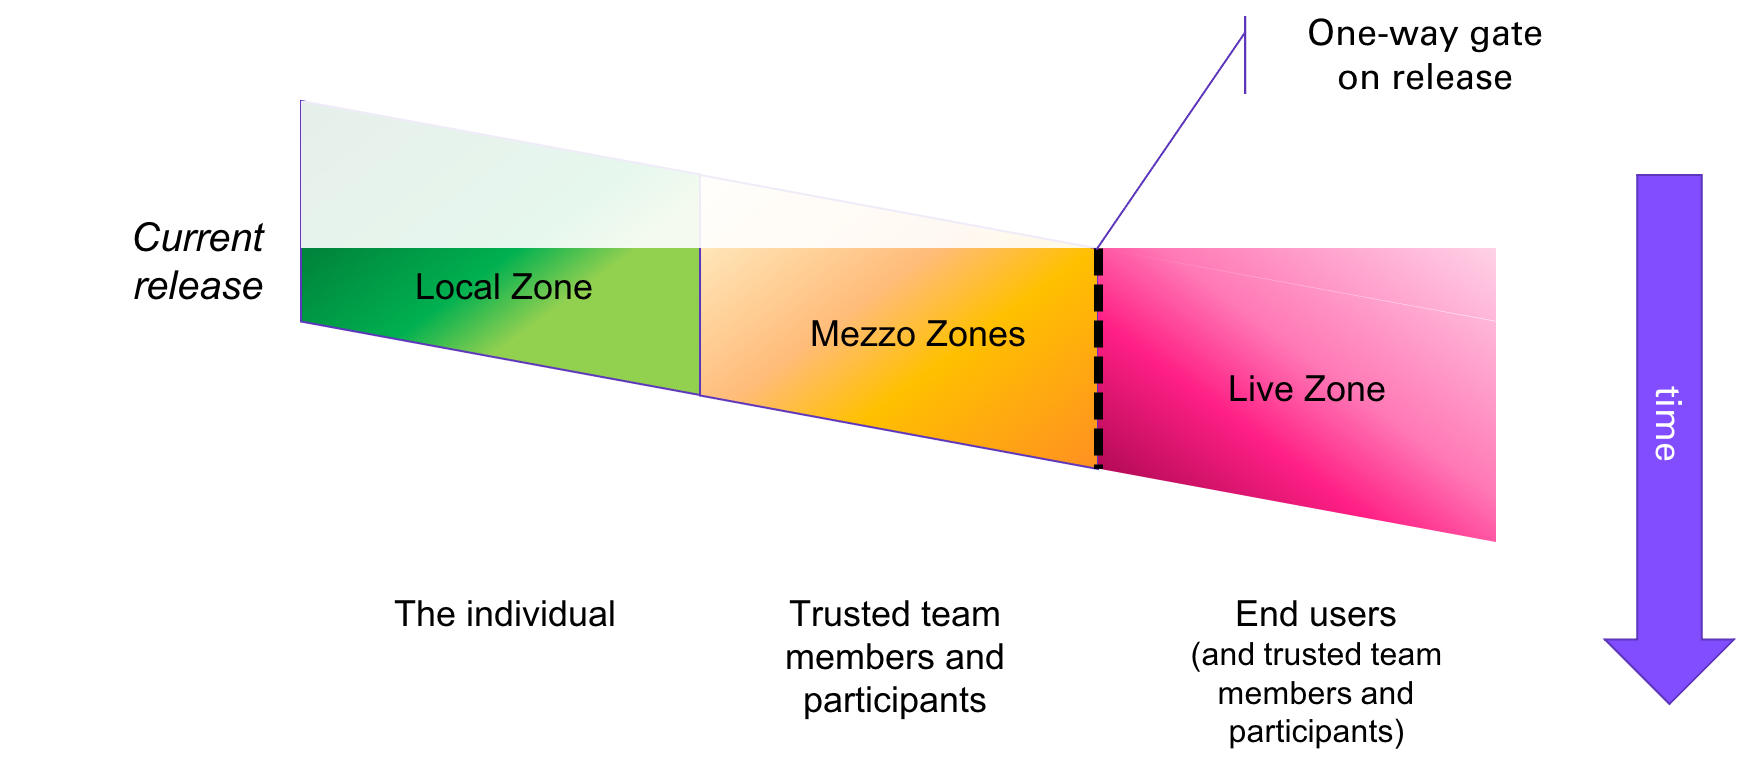
\includegraphics[width=13cm]{images/my/control-find-fix-zones-a.png}
    \caption{Control find-fix zones}
    \label{fig:my:control-find-fix-zones-overview}
\end{figure}

These three categories of zones are illustrated in Figure~\ref{fig:my:control-find-fix-zones-overview}. The figure includes a one-way gate, that behaves like the Rubicon in Julius Caesar's time~\citep{wikipedia_rubicon} where the die is cast once a release has been launched in the app store. The release cannot be reverted, at best it can be paused or superseded with another subsequent release. The app now comes into contact with end-users and is expected to achieve the business objectives of the organisation who made it available.

\begin{figure}[htbp!]
    \centering
    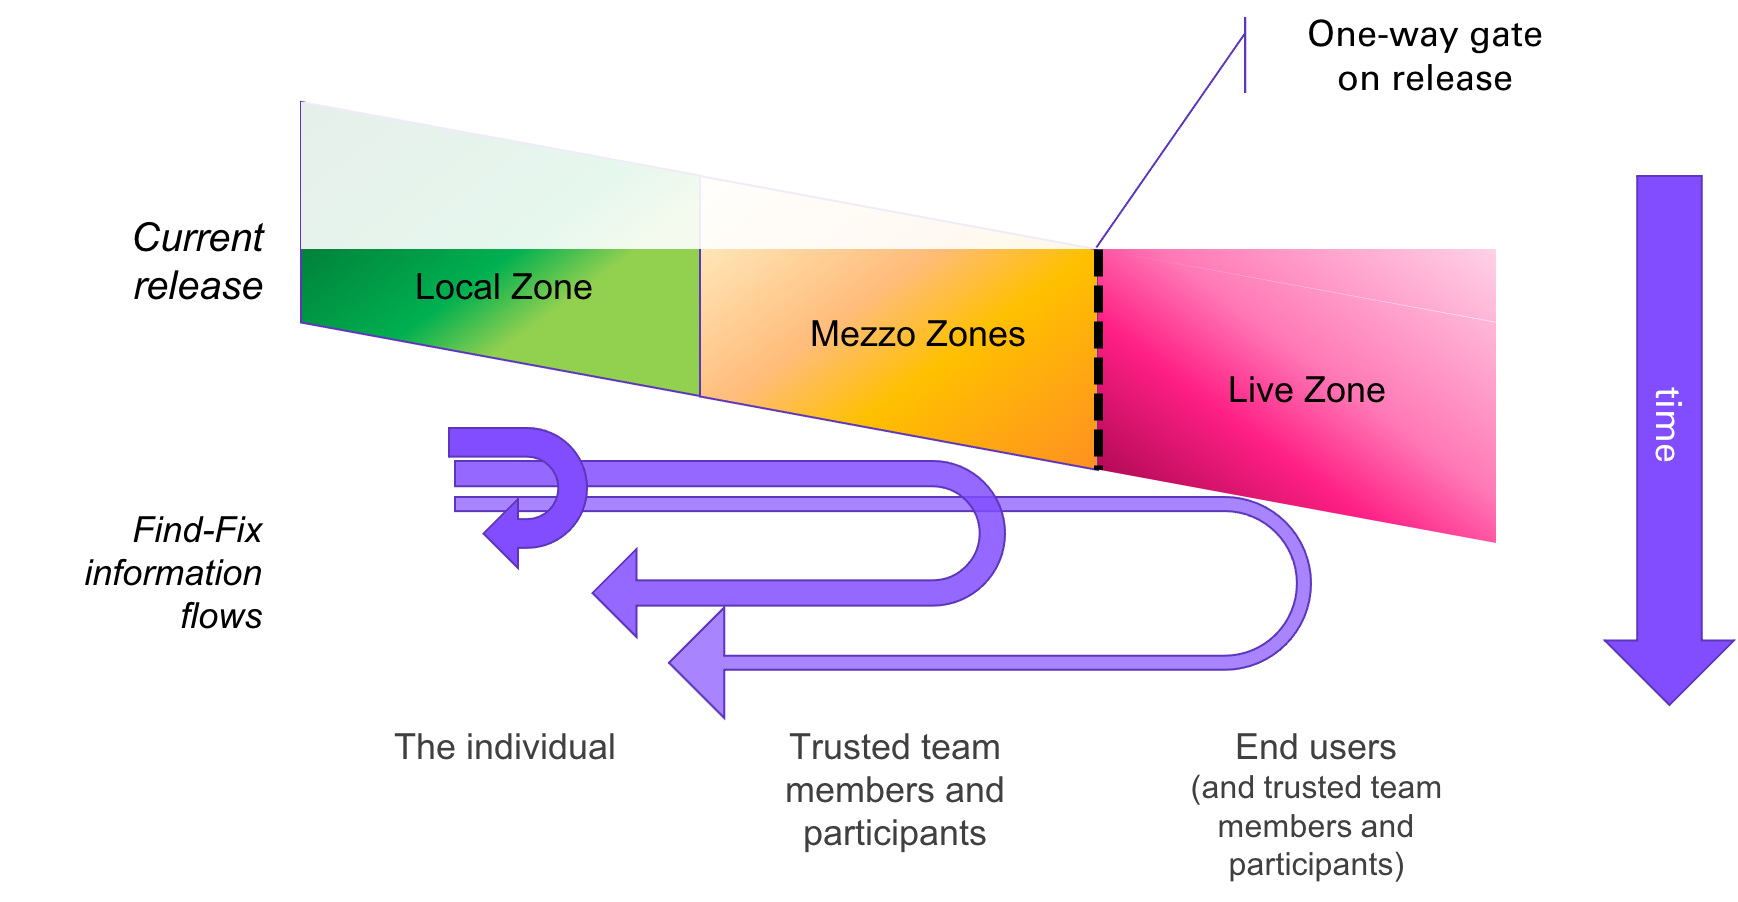
\includegraphics[width=13cm]{images/my/control-find-fix-zones-with-information-flows.png}
    \caption{Control find-fix zones with information flows}
    \label{fig:my:control-find-fix-zones-with-information-flows}
\end{figure}

Figure~\ref{fig:my:control-find-fix-zones-with-information-flows} is a modified version of Figure~\ref{fig:my:control-find-fix-zones-overview} that includes the find-fix information flows. Assuming fixes are made be the development team for the app (rather than improvements that can be addressed in servers, through configuration changes, and so on) then the information about flaws and issues needs to reach that development team somehow. For issues found in external releases (\emph{i.e.} those made available to end-users) 


When issues are discovered before the software is released there is the possibility of the developer being able to address them before the software is released (they stakeholders may choose to delay the release to allow this to happen). Where issues are discovered in the released app, unless there are viable mechanisms to patch the app, the fix needs to be made in a subsequent release \textit{and} the end-user needs to use the subsequent release to receive the benefit of the release.

There are two key challenges:
\begin{enumerate}
    \item the developer learning about issues in sufficient detail to potentially address them,
    \item being able to address issues and provide the benefit to users who are, or  may be, affected by it.
\end{enumerate}

Both these aspects are covered next in terms of the bug-fix process for mobile apps.

\subsection{Bug-fix process for mobile apps}
%MUST-DO move the following comment to the next chapter once I've drafted the relevant illustrations.
% In my view, mobile analytics helps in the 'current' timeframe of the development and release process, in that it can provide ranked notifications of various issues (including 'stability' failures: i.e. crashes and ANRs) on a timely basis. 

Given apps have been released and users are using those releases then - there may be issues in the app exposed while it is in-use. Some of these may be noticeable (or perceivable) by the end-users, others not. These issues include 'stability' failures: \textit{i.e.} crashes and ANRs and performance-related issues \textit{e.g.} slow responses, excessive power and network consumption, and so on.

For the development team to actively address any of these failures they need to be aware of them and have sufficient details to take action. Figure~\ref{fig:my:bug-fix-process-for-mobile-apps-in-prod} illustrates past, current, and future, activities for current and future releases of an app. We will return to this figure %in this section and 
in the next chapter where the effects of applying analytics to the development process is considered.
%MUST-DO make sure I do return to {fig:my:bug-fix-process-for-mobile-apps-in-prod} in the next chapter, on applying analytics.

\begin{figure}[!htbp]
    \centering
    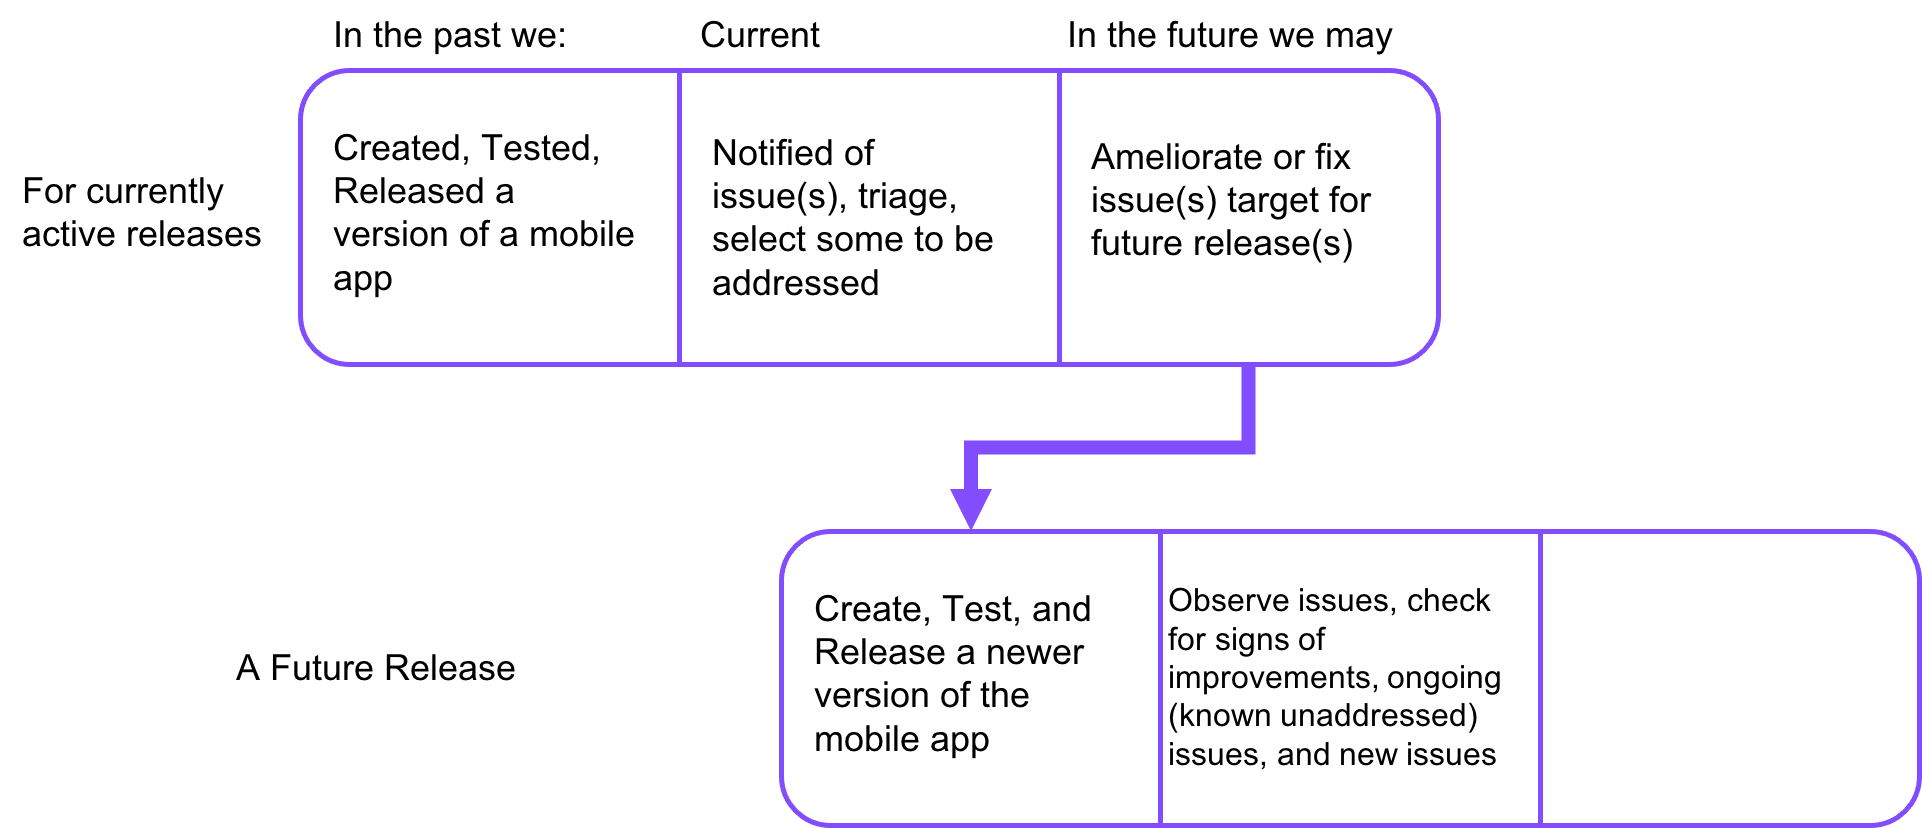
\includegraphics[width=13cm]{images/my/production-bug-fix-process-for-mobile-apps.png}
    \caption{Bug-fix, process for mobile apps in production}
    \label{fig:my:bug-fix-process-for-mobile-apps-in-prod}
\end{figure}


Developers might learn of some of these issues from other sources e.g. from colleagues who use the app, from end-users who report issues (e.g. in reviews in the app store, on social-media, and even using in-app feedback if the app's functioning sufficiently etc.). 
% MUST-DO refer to research in automatically creating automated tests to reproduce crashes and discuss some of the limitations of that research vector. Note: this might be covered in the related works chapter.
However in my experience, and based on other research, only a subset of the issues are reported by people who use the app, and certainly not all users report all the stability issues all of the time.

Any amelioration or fix that occurs in the app's codebase is only useful to those users who use the newer release of the app that include the improvements. Our research confirms some users continue using older releases of the app unless blocked/prohibited from doing so (there are mechanisms for doing so). Blocking/prohibiting use of older failing versions of the app may be a mixed blessing. Some users may be lost and/or upset by being forced to upgrade the app. However the stability stats in the app store may improve (assuming the intended improvements were effective).


\section{Conceptual model of apps and app stores}
This section introduces a conceptual model of apps and app stores and presents four views of apps in an app store together with various implications of the views, relationships and interactions. 

The vast majority of mobile apps are provided through app stores, and the two largest app stores:~\href{https://play.google.com/store/apps}{Google Play} and Apple's~\href{https://www.apple.com/app-store/}{App Store} both collect mobile analytics from end user's devices with permission. So, understanding the conceptual model of apps and app stores provides some context for these sources of mobile analytics. 

The research is situated in apps that are available in app stores. App stores house millions of apps and serve billions of users. They also present a rich tapestry of perspectives on software apps and the ecosystem. There has been a great deal of research that focus on particular areas of these apps and sometimes connect these areas as part of the research. This research focuses on an area seldom investigated, namely it concentrates on the developer's view of how their app is perceived by the app store and whether they can improve the perception by addressing sources of failures.

\begin{figure}[htbp!]
    \centering
    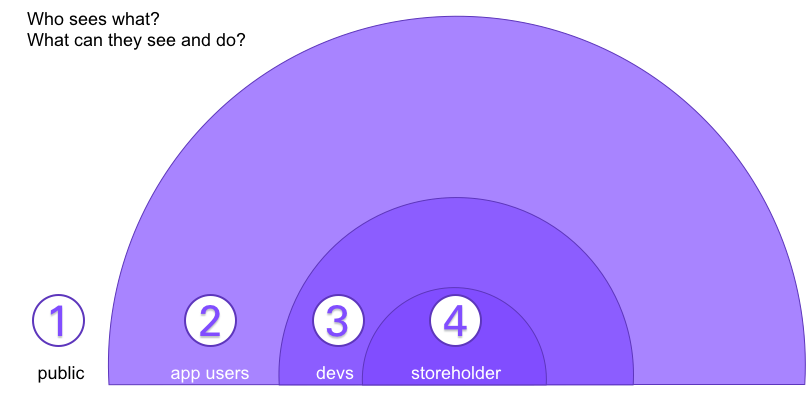
\includegraphics[width=12cm]{images/who-sees-what.png}
    \caption{Four Views of an App Store}
    \label{fig:4-views-of-apps-in-app-store}
\end{figure}

Figure~\ref{fig:4-views-of-apps-in-app-store} illustrates the four views; broadly, those closer to the centre can also see what those in outer rings can see. As a wise supervisor commented: \emph{``It's a bit like standing at different elevations on a mountainside and looking out over the landscape - the higher you are, the more you can see"}.

The first view is the public view of the app store, what is visible to someone who is not actively engaged with the app store. Examples include people who are not logged into their account, search engines, researchers mining the app store for ratings and reviews, and so on. The public is able to see aggregate ratings and some recent reviews for specific apps. Older reviews are generally hidden from public view (which may limit some research and search engine insights).

The next view is that of a user of a particular app or set of apps. They may have installed some of the apps directly, they are likely to also have pre-installed apps on their device too. They have the ability to interact with the app store, for instance they can see, create, and update their ratings and reviews~\footnote{If supported by the app store, for instance Google Play does.}. They can also see the public view.

%\akb{In the sentence below, does '.. records about their interactions ...' refer to the interactions of the developer or the user?}
Developers have the next view, which includes information the app store records about the developer's interactions with the app store, and information the app store provides the developers directly (\emph{i.e.} generated by the app store and related entities), as well as feedback provided by users via the app store (\emph{e.g.} ratings and reviews). Developers can also see the public view, although they cannot see the entire view of their user-base. However they can see any rating and reviews provided by the users.

%\akb{Do we know why the qualified 'often' is needed in the next sentence? Is this a non-deterministic behaviour of app stores and hence a forewarning of some of the data quality issues in the analytics platforms?}
Authors and developers are the two end points of ratings and reviews. Authors create them and developers receive them and can choose to respond to them, at least in some app stores. %these conversations. 
Importantly, their primary communications goes via the app store, rather than being direct, and aspects of these communications are often public for a period. Authors and developers can see their individual ratings and reviews for much longer periods than presented in the public view. The app store can use the ratings to decide on the quality of the app and their assessment may affect various important facets of the app's existence in the app store. For instance, well rated apps may be promoted and poorly rated apps may be demoted in search results. As Google states~\emph{``Apps whose metrics are higher have greater promotability, which raises their ranking in Google Play Store searches."}~\citep{android_vitals_best_practices} Also, poorly rated apps are sometimes subject to additional scrutiny and delays in the release process, as illustrated in Figure~\ref{fig:pocketpaint-to-help-better-protect-users} when the overall rating for a release dropped sufficiently to trigger this change. % The communications and implications will be covered later in this section.

\begin{figure}[htbp!]
    \centering
    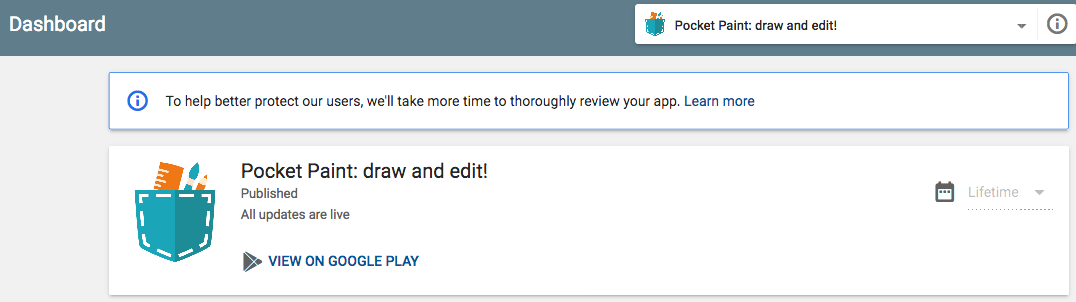
\includegraphics[width=15cm]{images/android-vitals-screenshots/pocketpaint-to-help-better-protect-users.png}
    \caption{Google Play message for Pocket Paint: To help better protect our users...}
    \label{fig:pocketpaint-to-help-better-protect-users}
\end{figure}

The final view is that of the app store, the `storeholder' in the figure. They have a global and holistic view of the entire store, including \textit{potentially}\footnote{A caveat on the use of potentially: this is because the app stores are closed systems with limited information about their actual behaviour in the public domain.} all the reviews, user interactions, and whatever usage activities have been performed by all the other three views. 
%\akb{Some explanation of the caveat term 'potential' here would be useful I think - i.e. this is because the app stores are closed systems with limited information about their behaviour in the public domain?}

We now cover various implications of the app store conceptual model.

\subsection{Trust relationships}
One of the key success factors of the modern app store (typified by the Apple App Store and Google Play) was that the platform provider provided the entire ecosystem and established the rules of engagement. The locus of trust is the provider of the app store, which acts as the public face and to some extent also acts as a representative for both the users and the developers. In terms of financial transactions it also acts as the intermediary and facilitates users being able to obtain refunds for app and in-app purchases subject to various conditions. 

Note: There are many details related to the trust relationships for those interested in that topic, however in the interests of focus and concision they are outside the scope of this thesis. 

\subsection{Communications paths and data flows}
There are numerous communication paths for mobile apps both with and without an app store being involved. As the vast majority of apps and users use devices and apps that are part of an app store ecosystem (even if they are obtained from other sources, e.g. as often occurs in India) I will only consider the ecosystem that includes an app store in this thesis. Figure~\ref{fig:sources-of-info-with-app-store-background-ch} illustrates various sources of information for apps available in an app store. The sources and communications paths will be considered next. 
% SHOULD-DO Perhaps a Venn diagram would also complement this illustration?

\begin{figure}[htbp!]
    \centering
    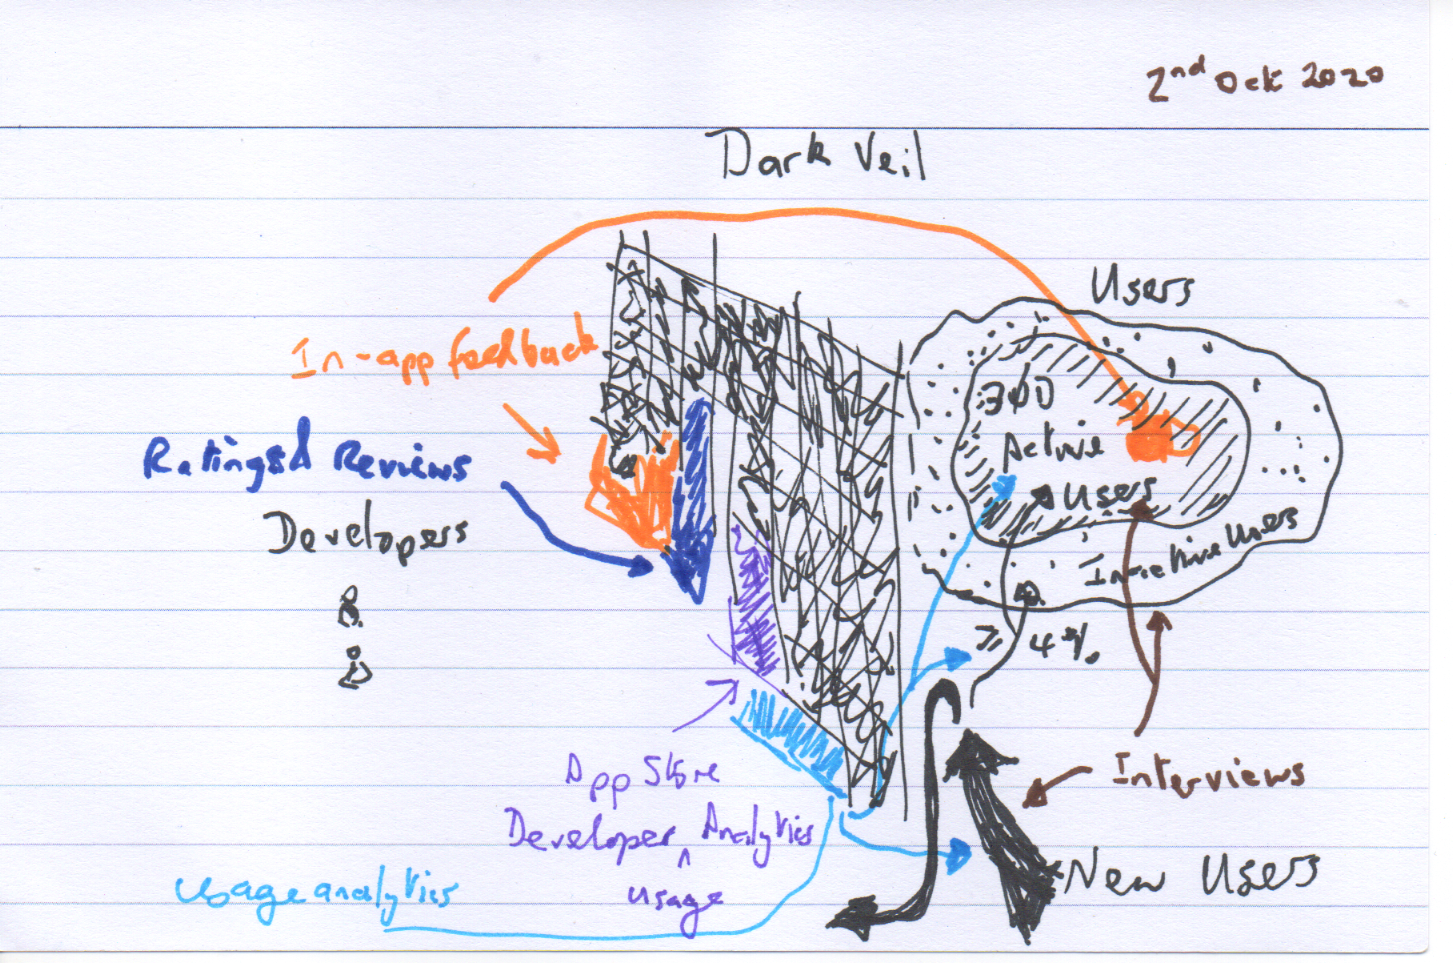
\includegraphics[width=13cm]{images/rough-sketches/sources-of-information-with-app-store-1.png}
    \caption{Sources of information with an App Store}
    \label{fig:sources-of-info-with-app-store-background-ch}
\end{figure}

The information about mobile apps can come from users directly or indirectly, from the app if it collects information either directly or indirectly, from devices. Such data collection could be via the operating system, installed apps with privileges to access information about other apps, from accessibility services, and potentially other means e.g. installed viruses. Alternatively, it could come from intermediaries - particularly the app store, and also from network traffic, observers,~\emph{etc.} 

Source code and source code repositories are also useful sources of information about mobile apps. Information can be usefully combined from several sources, for instance from source code about calls to write log messages compared to actual logs recorded when the app has been used on a device. Given the app store plays a pivotal role let's consider its role in terms of communication paths now. 

An app store is more than the store front, it controls and affects many aspects of the ecosystem that gathers around it. It is also more than the software, data and information that the various memberships can access. For instance the modern app stores often include software that is mandatory and pre-installed on end-user devices where that software cannot be easily removed or disabled by users\footnote{competent, technically savvy individuals may be able to thwart protection mechanisms as may other specialist organisations and software.} . This software includes a local storefront that offers end-users new apps, updates, and enables users to manage optional apps\footnote{Optional apps can be installed and uninstalled by end users at will. Non-optional apps are installed by various organisations, including the app store provider, some device manufacturers, and so on.}.

The app store provides various primary communications paths between the various parties involved in the ecosystem. It may be an active party, for instance in some of the reports provided to developers and/or users, and in policy-related matters; or it manages communications between app users and developers. Often the app store's owners define the rules of communications, including details such as whether and when apps can ask users to rate an app.

\begin{figure}[htbp!]
    \centering
    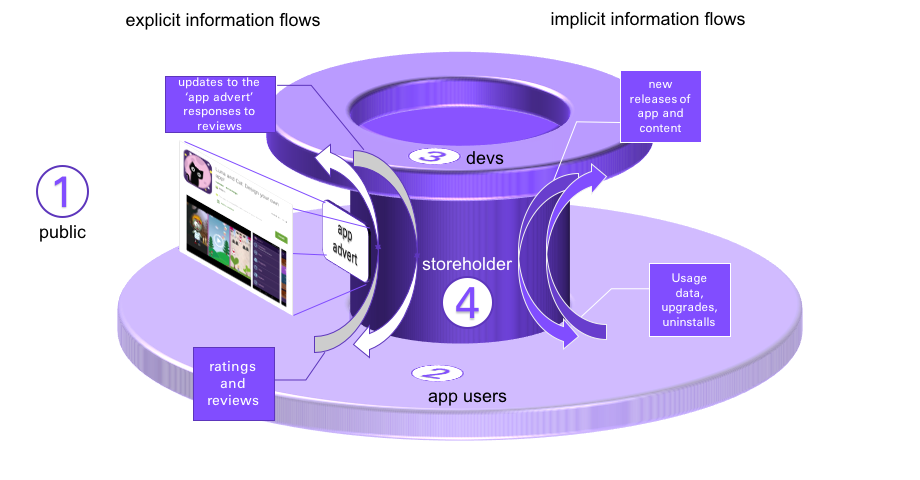
\includegraphics[width=17cm]{images/app-store-data-flows-3d.png}
    \caption{App Store: Communications Paths and Data Flows}
    \label{fig:app-store-data-flows}
\end{figure}

Some of the communications involves humans, or software chatbots masquerading as pseudo-humans intended to behave similarly to how humans would do in similar circumstances, for instance to provide in-app assistance~\citep{baez2020_chatbot_integrations} and to help developers respond automatically to app reviews~\citep{greenheld2018_automating_developers_responses_to_app_reviews}. Other communications is generated by software, for instance usage and diagnostic data collected by the operating system and related utilities on a mobile device (collectively described as the platform).

%\akb{Why are bots characterised as 'pseudo-humans'?}

The communications paths and data flows in an app store ecosystem are illustrated in Figure~\ref{fig:app-store-data-flows}. There are two forms of data flows: explicit and implicit. Explicit data flows are actively and intentionally performed by one or more of the participants, implicit data flows represents information that can be inferred or gleaned from various actions and inactions.

Examples of actions intended to communicate explicitly include:
\begin{itemize}
    \item Making the app available in the app store; this includes creating screenshots, a description of the app, adding meta data the app store requires and/or requests, \emph{etc.} This information becomes public if the app store approves the app for release.
    \item Ratings and reviews performed by app users. Only a subset of users provide these, the percentage varies from zero to a maximum of around 10\% with typical percentages around 1\% to 3\%. % SHOULD-DO find credible source for these estimates, I've checked various sources without success
    Estimates vary, partly as the definitions vary too. AppBrain states 46.5\% of Android apps do not have a rating~\footnote{Their definition is \emph{``Apps that have less than 3 ratings we consider to not have a rating yet"}~\url{https://www.appbrain.com/stats/android-app-ratings}}. In comparison, 42matters.com estimate 41\% of Android apps and 57\% of iOS apps have no rating~\footnote{\url{https://42matters.com/stats}}.
    \item Responses to reviews, for example Google Play allows developers to respond to reviews, and for both reviewers and developers to update their reviews and responses.
    \item Suspending an app so it is no longer available to users to download. Storeholders sometimes suspend apps and even developer accounts where they perceive the app and possibly the developer contravenes the app store's policy. % c.f. the recent ban of Fortnite in both Apple and Google stores. And see the comment after this article re German law https://www.overpass.co.uk/google-play-account-suspended/ 
    %\href{https://www.ape-apps.com/viewpage.php?p=34186}{My Colony Suspended from Google Play}
    %\href{https://www.ape-apps.com/viewpage.php?p=34173}{My Colony removed from Google Playstore} - over 50% of users come from Google Play.
    
\end{itemize}
%%%%%%% Various interesting sources of Android- (and some iOS) related stats
% https://www.businessofapps.com/data/app-statistics/
% https://www.statista.com/statistics/266217/customer-ratings-of-android-applications/ (seems to be a rehash of AppBrain's report)
% https://mindsea.com/app-stats/
% 

%\akb{Use consistent labels for concepts - below you refer to '(implicit) information flows' whereas above you use '(explicit) actions intended to communicate'.  By using different labels you are suggesting that these two implicit/explicit categories are not directly comparable, i.e., they are different types of things altogether. However, I am not sure this is your intent.}

Implicit information flows include:
\begin{itemize}
    \item New releases of apps and related content (such as in-app content, often purchased using in-app purchasing). These indicate the developer is wishes to actively engage their userbase. Upgrades may include changes to the app seeded by various sources such as ratings and reviews and other data, including:
    \item Usage data and upgrades, both imply the software provides some value to the users. Lack of usage may also be an indication the software is not currently providing value - this may be expected for instance with seasonal apps. Uninstalls are a stronger signal that users no longer see sufficient value in the app to keep it on their device.
\end{itemize}

On-device bug reports may be a hybrid, where the bug reporting utility on the device does much of the data collection and may report this automatically and transparently, however it may sometimes ask the user for additional input and permission to send the bug report.

\subsection{Membership criteria of each group}
%\akb{Explain why the membership criteria are important to understand, perhaps combine with next section single explanation of groups and what members can do in each}
As Figure~\ref{fig:app-store-data-flows} illustrates there are four numbered groups in the illustration. People can potentially belong to more than one group (albeit membership of the storeholders is limited to owners and those they assign membership to,~\emph{e.g.} as administrators of the app store). Group membership constrains what the members can do as participants and what they have access to.

\begin{enumerate}
    \item Public: the membership criteria are minimal. Here `public' is any entity, human or technological, that has access to the app store\footnote{For our purposes we can assume online digital access, other modes may also be viable, for instance some researchers use archives of data sourced from app stores.}. An example of a technological entity, is a search engine crawler or software including web scraper technology and scripts that use APIs provided to obtain information about apps in the app store.
    %\akb{Not sure what is meant by 'minimal' here. You could describe 'public' as any entity, human or technological, that has access to the app store. Provide an example of a technological entity, e.g., a search engine crawler}
    \item App user: the public can use an existing account or create a new account with the app store that would allow them to become an app user~\footnote{They need to meet the criteria of the app store.}. Note: there may be restrictions or constraints that mean not everyone can install every app on every device, however the general practice is that apps are freely available for app store users to install on any device they possess. 
    \item Developer: developers need to be registered and validated by the app store, the process varies for specific app stores, they often involve payment of a fee and some amount of validating their identity. Some app stores may perform additional checks based on information they and/or others hold.  
    \item Storeholder: they are generally a legal entity, and certainly for the purposes of this research they are. Apart from a few exceptions (such as F-Droid~\footnote{Details are available online at~\url{https://www.f-droid.org/en/about/}}) they are multi-national major corporations.
\end{enumerate}


\subsection{What participants can and cannot do (and who dictates the rules?)}
%\akb{You don't explain the link between the implicit/explicit data flows and these membership groups.}
\begin{itemize}
    \item Public: The public cannot review an app or easily download the app. They can view publicly accessible information, including information that was gathered previously, potentially by others.
    \item App user: They can rate and review apps they have installed on their account~\footnote{ user may have several devices and choose not to install an app on all of them. Also some apps may by limited to devices that meet particular criteria e.g. the platform version.} or device. They can also install, update and deinstall apps~\footnote{There may be restrictions imposed for some apps, for instance Google Apps and Manufacturer apps might be blocked from being uninstalled, and updates are sometimes mandatory, \emph{etc.}}.
    \item Developer:  Approved developers can upload apps to the app store and publish them if the app store also approves the release. They can choose to submit new versions of their apps, sometimes they may be required to do so by the app store. They can choose to suspend or withdraw their app from the store, note: generally users can continue to use the app if they have it installed. Developers are expected to interact with the app store and often do so of their own volition, for instance to see how their app is `doing'. The developer may define a price for their app and/or any in-app purchases. They may also require users comply with additional terms of use, and many apps do so.
    \item Storeholder: They are by far the most powerful participant as they establish the ecosystem including the rules of engagement and enforce these rules. The app store has the right of delay or veto of releases, it can suspend apps and developers, and much else besides. They are expected to comply with the laws of the various countries the app store is available in and also where their business is situated. These laws may affect the developers and the app users, for instance the amount of sales tax charged on a purchase in the app store.
\end{itemize}

We have already identified four membership groups involved in app store ecosystems, there is at least one more and also additional data flows in the ecosystem. The fifth membership group is a~\emph{service provider}. These service providers provide non-trivial functionality and other capabilities such as in-app analytics, feedback, and so on. Developers can choose to incorporate software libraries into their apps and use the services provided, for instance as conduits of communications between the app and the developers. Here developers include other specialist groups in their organisation such as customer service personnel and marketing teams. Many app developers choose to use at least one such service, some incorporate several and there is even specialist software that enables developers to manage multiple similar services within their apps on end-user devices. An example of this type of software is~\url{https://github.com/segmentio/analytics-android} (other platforms are also supported and there are other providers of similar software).

Membership matters in particular because of who has access to which data and for how long they have access. Note: Control and `ownership' of the data are also relevant topics, however they are not necessary to comprehend the rest of this topic. % SHOULD-DO consider whether to add material on this topic in the thesis. 

\section{Conceptual model of layers within apps and observation points}
Observation can be internal,~\emph{i.e.} built into apps, and external. External includes instrumentation, debugging tools, the operating system at runtime, accessibility interfaces, event listeners, log watchers, and so on (as this is not intended to be an exhaustive list). The observation may also be indirect, for instance using network monitoring software, and/or from remote APIs, REST endpoints, and web servers (with their attendant logging).

\subsection{Three layers of an app}
In earlier work, published in ~\citep{harty_aymer_playbook_2016}, the concept of three layers of an app was introduced. These are illustrated in Figure \ref{fig:3-layers} and shows three primary conceptual layers related to a mobile app. 

\begin{figure}[htbp!]
    \begin{minipage}{\textwidth}
    \centering
    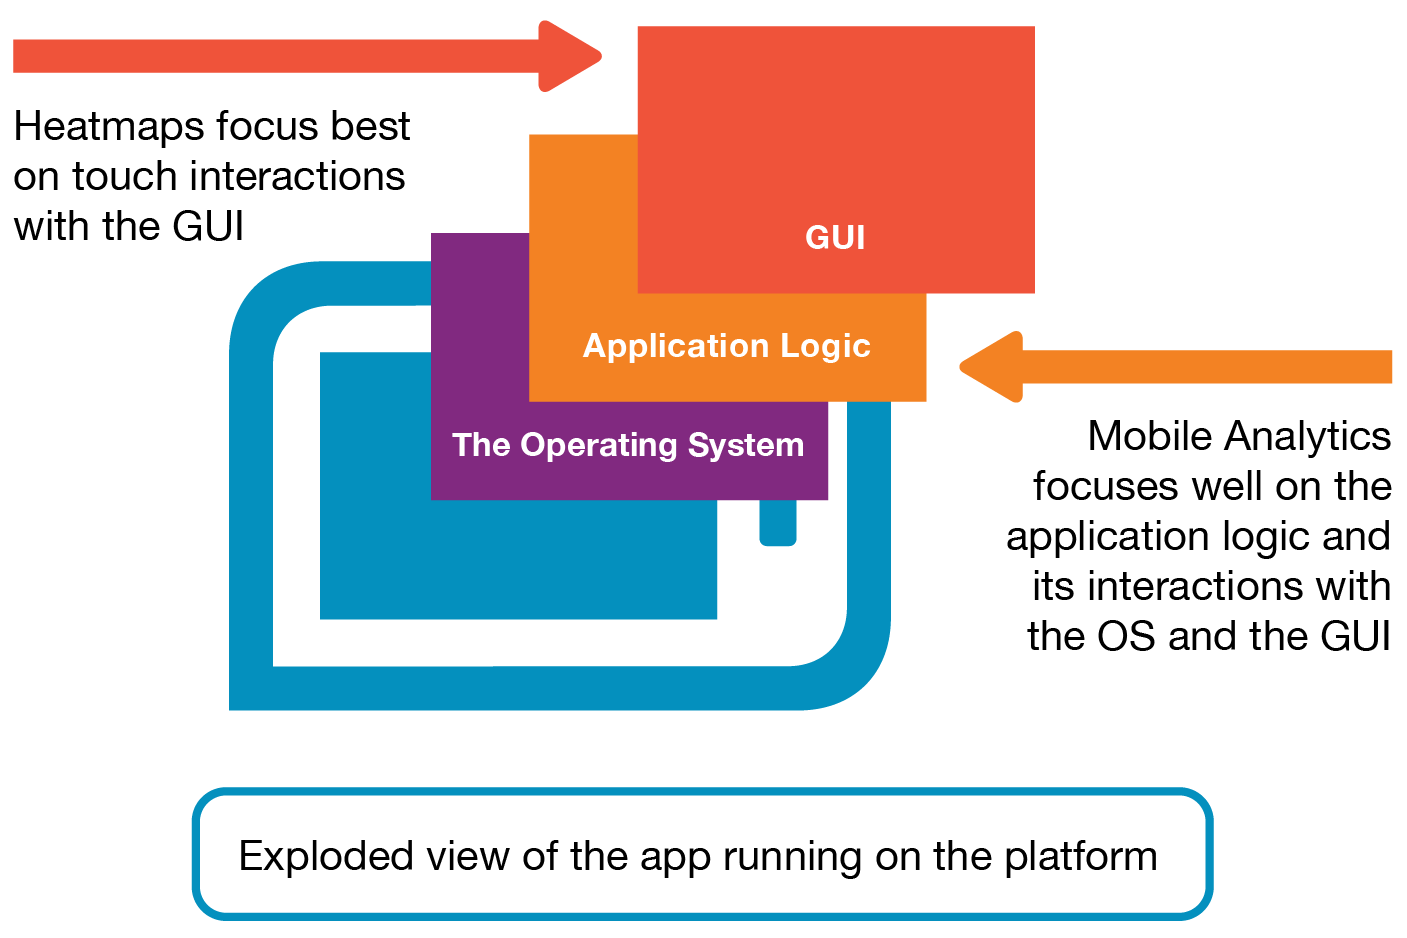
\includegraphics[width=10cm]{images/mobile-analytics-playbook/3-layers.png}
    \caption[Three layers of an app]{Three layers of an app~\footnote{Image credit: First published in The Mobile Analytics Playbook~\citep{harty_aymer_playbook_2016}}.}
    \label{fig:3-layers}
    \end{minipage}
\end{figure}

Of course, apps aren't quite this simple or well defined in reality, for instance they include software libraries from various sources, A/B testing utilities, logging code, run-time lifecycle management, and so on. Nonetheless, these three layers are a useful abstract, particularly in terms of useful observation points about apps on user's computer devices~\footnote{Another observation point that was orthogonal to the application logic layer was one popularised by a company that has since been acquired, called SafeDK. They provided app developers with software that provided an interface between the developer's code and the libraries the code used. This software collected and reported usage data on the performance and reliability of the libraries. Given the commercial nature of the business, their acquisition and the demise of their products and the company's website, and the fast moving nature of the internet, obtaining concrete information may be impractical for all but a few people who know those who were involved at the time.}.

The Graphical User Interface (GUI) % SHOULD-DO add to glossary.
can be visually observed by sighted users, it can also be observed by Accessibility software, and test automation tools, \emph{etc.} externally to the app. It can also be observed from within the app, for instance through using software known as \emph{heatmapping} that records the screens and the touch interactions performed by users of that screen. One of the the more popular, mature heatmapping offerings is from AppSee~\footnote{\url{  https://www.appbrain.com/stats/libraries/details/appsee/appsee}. Note: in 2019 Appsee's team was acqui-hired by ServiceNow~\url{https://techcrunch.com/2019/05/13/servicenow-acquihires-mobile-analytics-startup-appsee/} and the service no longer directly available.}, nonetheless they are only used in a small minority of mobile apps.


\subsection{Observation points: inside-outside perspectives}
The observation point determines what can be observed and how. 
As Figure~\ref{fig:internal-external-table} illustrates there are internal and external perspectives on an app for various purposes, including observations, interactions (e.g. through test automation), and emitting information (e.g. through logging, reporting, or mobile analytics). Where the information is observed affects what can be known and what is possible, an insider is privy to information an outsider is not; whereas an outsider has perspective and can potentially perceive things insiders cannot.

\begin{figure}[htbp!]
    \centering
    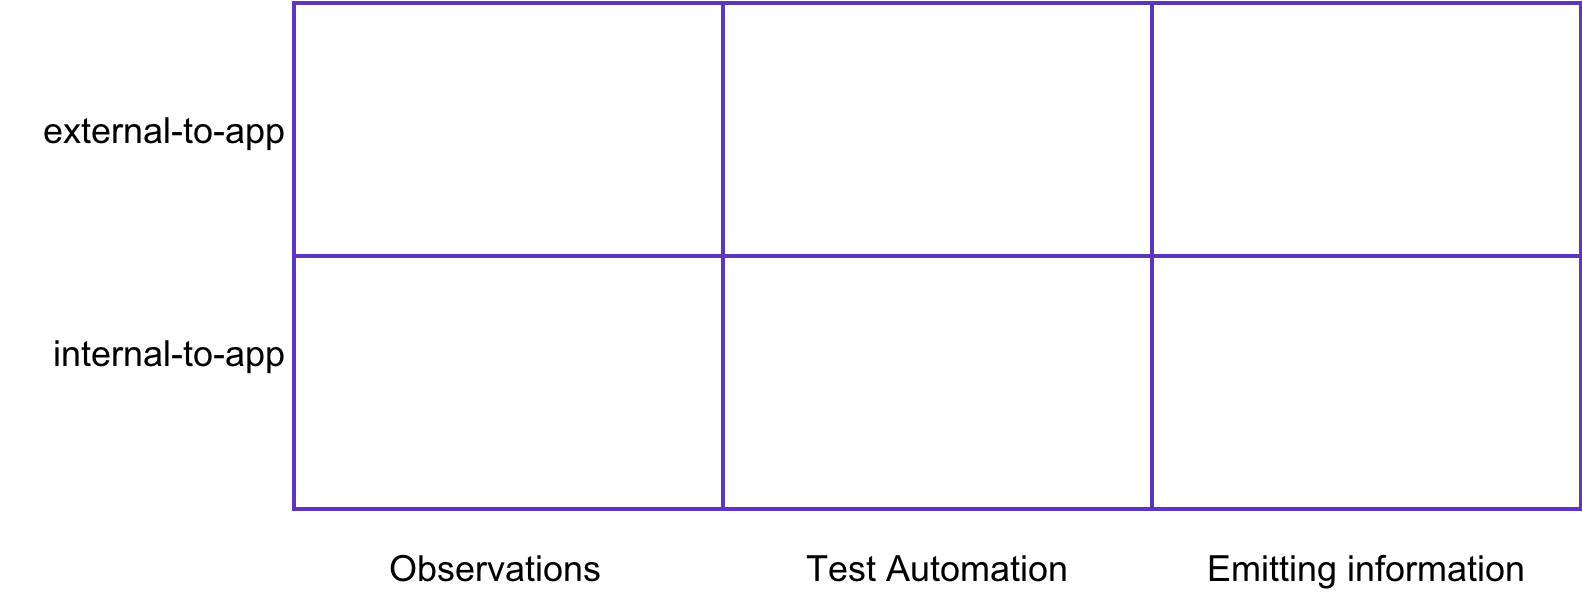
\includegraphics[width=13cm]{images/internal-external-table.png}
    \caption{Internal and external perspectives of an app}
    \label{fig:internal-external-table}
\end{figure}

%\textbf{SHOULD-DO} Expand the following: What is test automation? discuss how mobile apps are tested, the unique aspects of using accessibility interfaces, etc.

\section{Conceptual model of analogue and digital feedback}~\label{analogue-and-digital-feedback}
Feedback can help developers to find and choose ways to improve their software. Various researchers have investigated way to understand and use feedback provided by end-users, for instance, in ratings and reviews users provide to the app store. For the purposes of this research feedback people provides is considered~\emph{analogue feedback} as it has the richness and complexity of analogue signals, and also challenges of processing and comprehension.

In contrast, digital feedback originates from software and is generally deterministic~\footnote{~\url{https://en.wiktionary.org/wiki/deterministic}}. For the purposes of this research~\emph{digital feedback} is provided by running software where programmers added code to programs to collect data that provides feedback about software use and certain behaviours of that software. The addition of the code may be automated, in part, or wholly, for instance by another program or script. As an example, AppPulse Mobile claims they can add analytics automatically without developers writing a line of code~\footnote{~\url{https://www.microfocus.com/en-us/products/apppulse-mobile-app-apm-monitoring/overview}}.

\begin{figure}[htbp!]
    \centering
    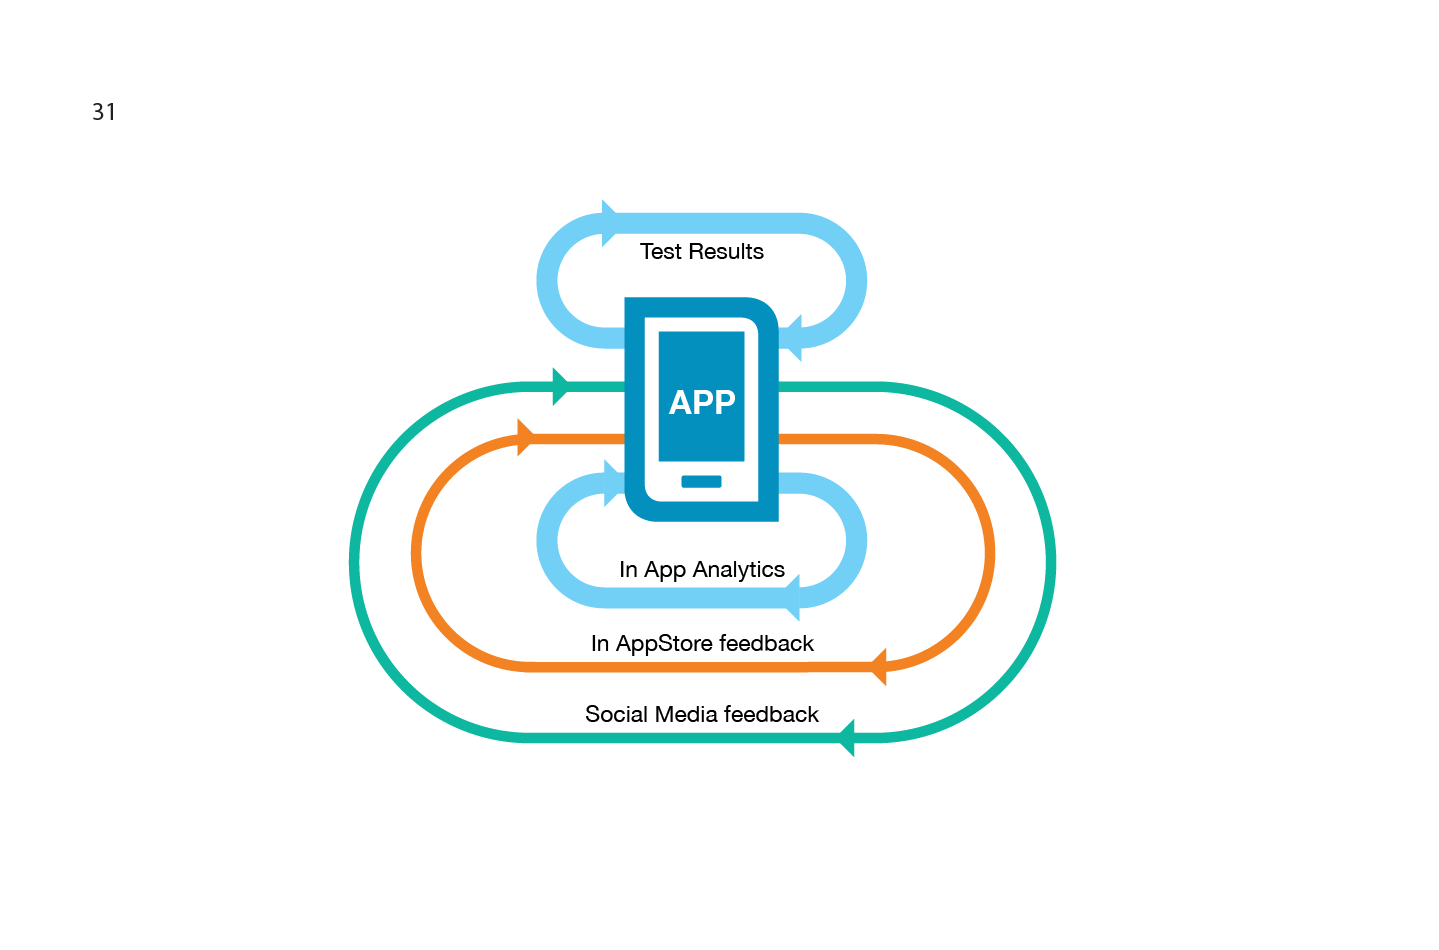
\includegraphics[width=15cm]{images/mobile-analytics-playbook/Chart-07-FeedbackLoops.png}
    \caption{Feedback Loops for mobile apps~\citep{harty_aymer_playbook_2016}}
    \label{fig:map2015-feedback-loops-for-mobile-apps}
\end{figure}
%SHOULD-DO edit the figure to remove whitespace, etc.

Figure~\ref{fig:map2015-feedback-loops-for-mobile-apps} illustrates various feedback loops where the feedback could be used to change and improve a mobile app. Within the team's aegis are test results (and static analysis, etc.). Beyond their direct control are feedback within the app, within the app store, and outside the app store ecosystem such as feedback on social media about their app. This figure illustrates in-app analytics which was the primary form of analytics at the time the figure was published, since then two additional forms of feedback have emerged: platform-level feedback such as Android Vitals and in-app feedback.

\subsection{Analogue feedback: in-app tools}
One source of feedback is when apps include feedback mechanisms within the app. Various benefits are touted to encourage developers to add such feedback including the ability to: ~\emph{``...capture valuable insights into the usability of the app and quickly resolve any issues..."}~\citep{mopinion2017_top11_mobile_in_app_feedback_tools}, for example. 

Some apps also collect in-app feedback if the user indicates they are not satisfied with the app and conversely ask users to submit a review online in the app store if they are satisfied. One hypothesis is their developers have implemented this approach to divert adverse ratings and reviews from public view and from the app store algorithms. 

In-app feedback enables a wider range of communications and also scope for richer dialogues than relying on feedback mechanisms provided by app stores which consist of a rating and an optional plain text comment. Examples of wider ranges of communications include surveys, and richer dialogues include audio recordings.

In-app feedback has also been proposed for bi-directional communications between developers and users of the app for instance to elicit non-functional requirements~\citep{avellis_harty_yu_towards_mobile_twin_peaks}.

\subsection{Analogue feedback: app store feedback}
App store feedback, combines a rating (typically using a one- to five- start rating and an optional plain-text comment). It is a subject covered by significant volumes of research and discussed in the related works chapter. %MUST-DO actually write up this related research and contrast it with mobile analytics.

\begin{figure}[!htbp]
    \centering
    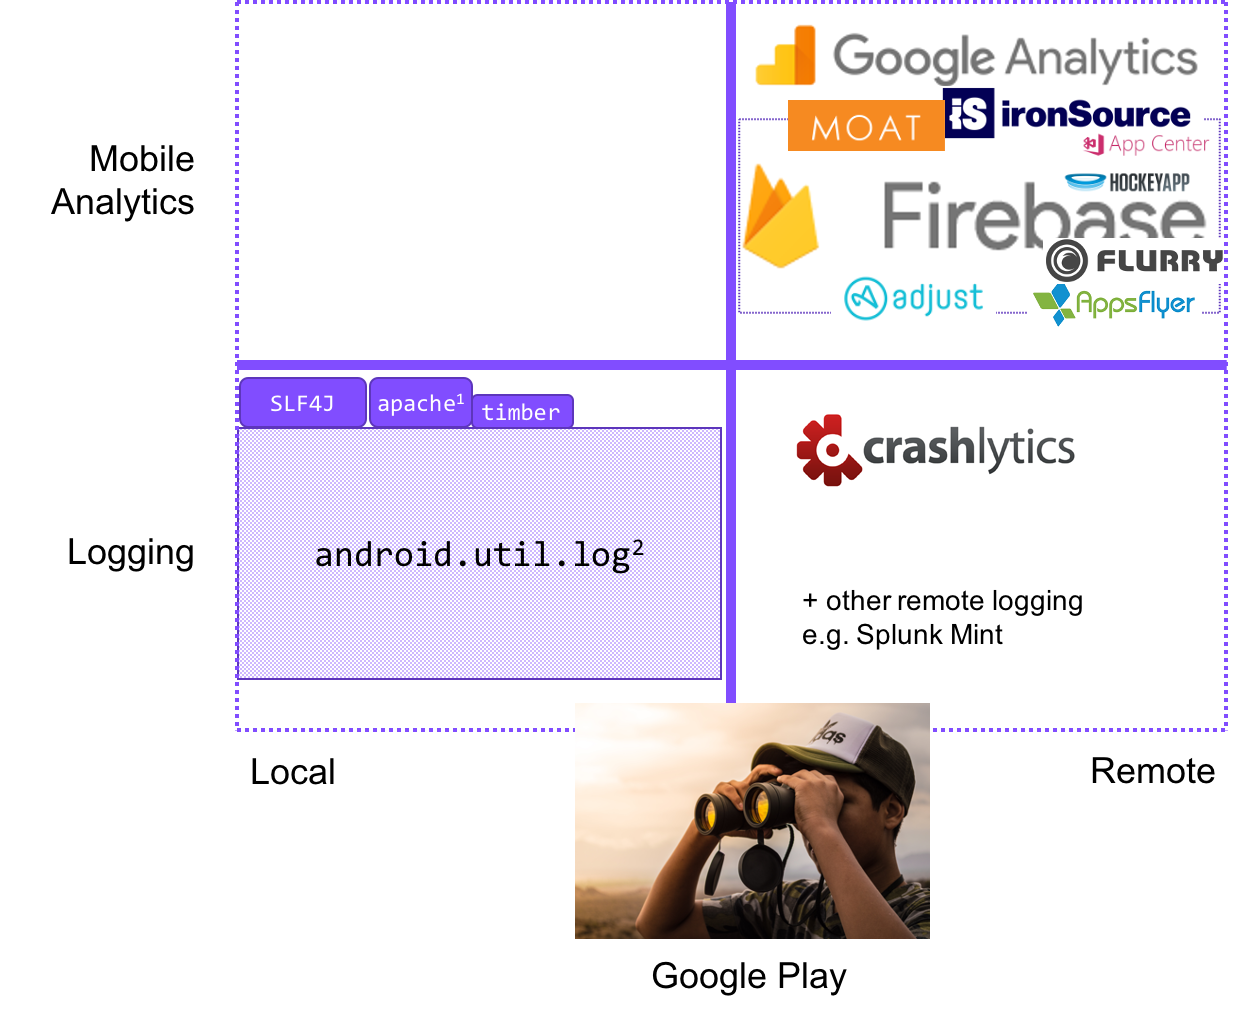
\includegraphics[width=12cm]{images/matrix-of-logging.png}
    \caption{Matrix of logging}
    \label{fig:matrix-of-logging}
\end{figure}

\subsection{Digital feedback: logging and mobile analytics}
The application may incorporate logging and/or mobile analytics. Logging in mobile apps is often used locally, by developers independently of other mechanisms. Mobile analytics is used remotely, as are crash reporting libraries. 



Figure \ref{fig:matrix-of-logging} illustrates a matrix of logging, where logging and mobile analytics are on the Y axis and local and remote on the X axis. There is a cross-cutting example where the mobile platform observes local events and then forwards the information remotely. A good example is Google Play which appears to be an external observer of data recorded in device logs. Data collection runs locally and is sent to Google servers where Google analyses the data and provides reports to developers for their apps. %SHOULD-DO check for related US patent filings by Google in this area.

\begin{table}[!htbp]
    \centering
    \begin{tabular}{lll}
         Category of logging &Local access?  &Remote access? \\
         \hline
         None            &N/A  &N/A \\
         \texttt{StdOut} &It depends &Unlikely \\
         Default platform logging library &Yes &Possible \\
         Enhanced platform logging library &Yes &Possible \\
         Third-party logging library &as-designed &as-designed \\
         Proprietary logging library &as-designed &as-designed \\
         
    \end{tabular}
    \caption{Choices available to developers for logging in mobile apps}
    \label{tab:logging-choices-for-devs}
\end{table}

Table~\ref{tab:logging-choices-for-devs} identifies various categories of logging available to developers of mobile apps. They range from no active logging in the app (some information is still logged by the platform) to proprietary custom logging libraries which a tiny minority of development teams would chose to do - they may do so to keep their logging as private as practical from the rest of the device.

\texttt{StdOut} is often used in code written for other platforms including Linux that has been ported to mobile platforms. Some people who are unfamiliar with logging libraries who have a superficial understanding of developing for mobile devices may also use print statements in their code (which effectively writes to the standard output) rather than use log statements in their code. There are various nuances of how the standard output and standard error outputs are handled in Android code (Java, Kotlin, etc.) and native code (C/C++) are directed as standard for Android apps. In short, for native code (\emph{e.g.} written in C/C++) as standard the outputs are discarded by `writing' them to~\texttt{/dev/null}. For Android code (\emph{e.g.} written in Java/Kotlin) \texttt{System.out} and \texttt{System.err} can be redirected to the log on some Android releases if the device is configured to do so.
%MUST-DO add references for https://github.com/android/ndk/issues/671 and https://codelab.wordpress.com/2014/11/03/how-to-use-standard-output-streams-for-logging-in-android-apps/ and https://stackoverflow.com/a/17199704/340175 and https://stackoverflow.com/questions/10531050/redirect-stdout-to-logcat-in-android-ndk

There are various enhanced log libraries, for instance~\texttt{timber} which are used by discerning app developers. These libraries also write to the platform log files. 

To Be Continued. %MUST-DO

\begin{figure}[htbp!]
    \centering
    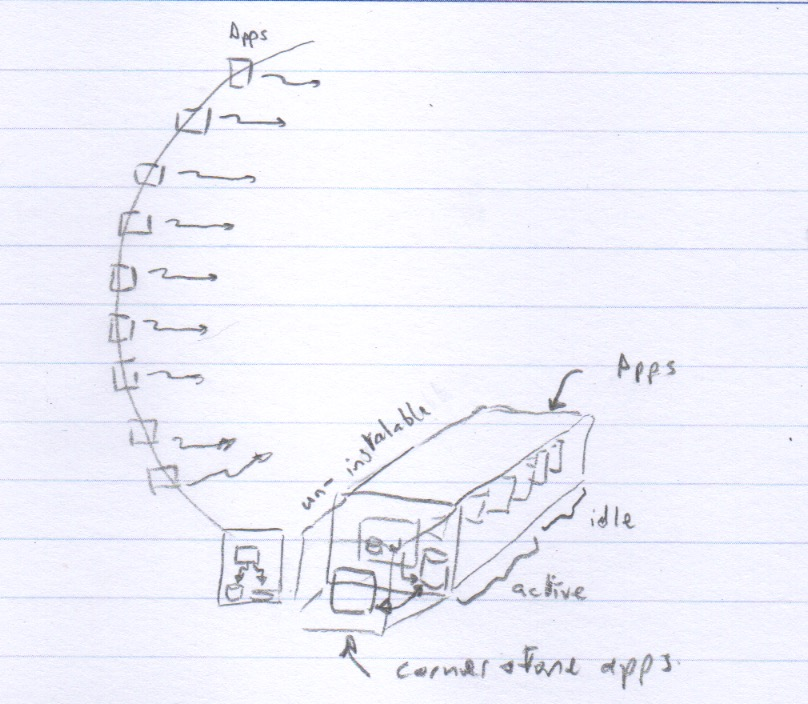
\includegraphics[width=12cm]{images/rough-sketches/apps-on-device-boundaries-sketch.jpeg}
    \caption{Apps on the device boundaries}
    \label{fig:apps-on-device-boundaries}
\end{figure}

\begin{figure}[htbp!]
    \centering
    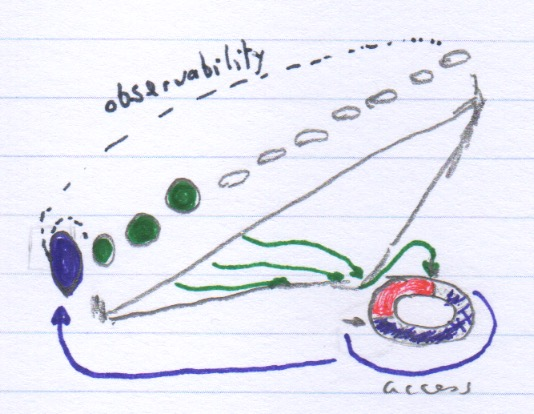
\includegraphics[width=8cm]{images/rough-sketches/on-device-logging-sketch.jpeg}
    \caption{On-device logging}
    \label{fig:on-device-logging}
\end{figure}

A couple of rough sketches, Figures~\ref{fig:apps-on-device-boundaries} and~\ref{fig:on-device-logging} present two views of apps installed on any given mobile device. These apps are broadly one of three categories: platform, pre-installed (non-removable), and user-installed (removable). Here the focus is on their use of logs on the device.

At any point one or more of these apps may be running, the rest are idle. The majority of these apps, with the possible exception of system apps, write to one or more shared, common, log files. These log files have a finite size, and once they are filled newer messages overwrite the oldest ones in turn. In Figure~\ref{fig:on-device-logging} the left-most blob, in purple, represents a system app that is able to read the shared system log files. These apps are pre-installed by the manufacturer, they may include those from the provider of the platform, particularly from Google for Android devices that use Google Play, and also some device manufacturers may have similar apps. Other apps are also pre-installed by manufacturers including a suite of apps from Google and some from the manufacturer. They may also include apps from organisations with agreements with the device manufacturer, for instance they may pre-install some games and utilities from partners. TBC.


As an observation the vast majority of Android developers use the default inbuilt logging library \texttt{android.util.log} and choose one or more of Google's analytics offerings (which include Firebase and Crashlytics). A commercial organisation, AppBrain, provides current statistics for third-party logging libraries~\footnote{Logging libraries (note the default android log library is not tracked at the time of writing~\url{https://www.appbrain.com/stats/libraries/tag/logging/logging-libraries}}, crash libraries~\footnote{\url{https://www.appbrain.com/stats/libraries/tag/crash-reporting/android-crash-reporting-libraries}} and mobile analytics~\footnote{\url{https://www.appbrain.com/stats/libraries/tag/analytics/android-analytics-libraries}}. Some apps have several of these libraries so counts may exceed 100\% in their reports.

\begin{itemize}
    \item Logging: enables developers to understand what their software is doing. The practice is commonplace across many software domains including mobile apps, and each platform and language includes a standard method of generating log messages. These messages tend to be small and intended for immediate, local consumption. On Android when developers use the standard logging library (\texttt{android.util.log}) their log messages are written to a shared circular log file on a device. As illustrated in Figures~\ref{fig:apps-on-device-boundaries} and~\ref{fig:on-device-logging}, some privileged Android software is able to read these shared logs. Developers can also read them using standard Android development tools \emph{e.g.} \texttt{adb logcat} providing they are connected to the device with the log file. Older versions of Android allowed apps to read the full contents, more recently apps are restricted to only the log messages they wrote unless they are granted the relevant permission by Google and the user. 
    In other domains \emph{e.g.} web servers, infrastructure software, and many others, logging is used for production monitoring, fault-finding and analysis. A minority of mobile app developers use remote logging.
    \item Mobile analytics, can extend and scale logging. For mobile analytics, a minority of developers incorporate custom implementations, however the vast majority who use analytics do so through using third-party analytics libraries such as Google Firebase Analytics, details of the current usage of analytics libraries are provided by AppBrain~\footnote{\url{https://www.appbrain.com/stats/libraries/tag/analytics/android-analytics-libraries}}.
\end{itemize}

One of the appendices, ~\href{appendix-on-mobile-analytics}{\textit{on mobile analytics}}, provides details of the design of content and messages together with the mechanics of sending the data; in terms of establishing a grounding in this topic it is enough to be aware that these are both relevant aspects of incorporating and using mobile analytics.


\begin{figure}[htbp!]
    \centering
    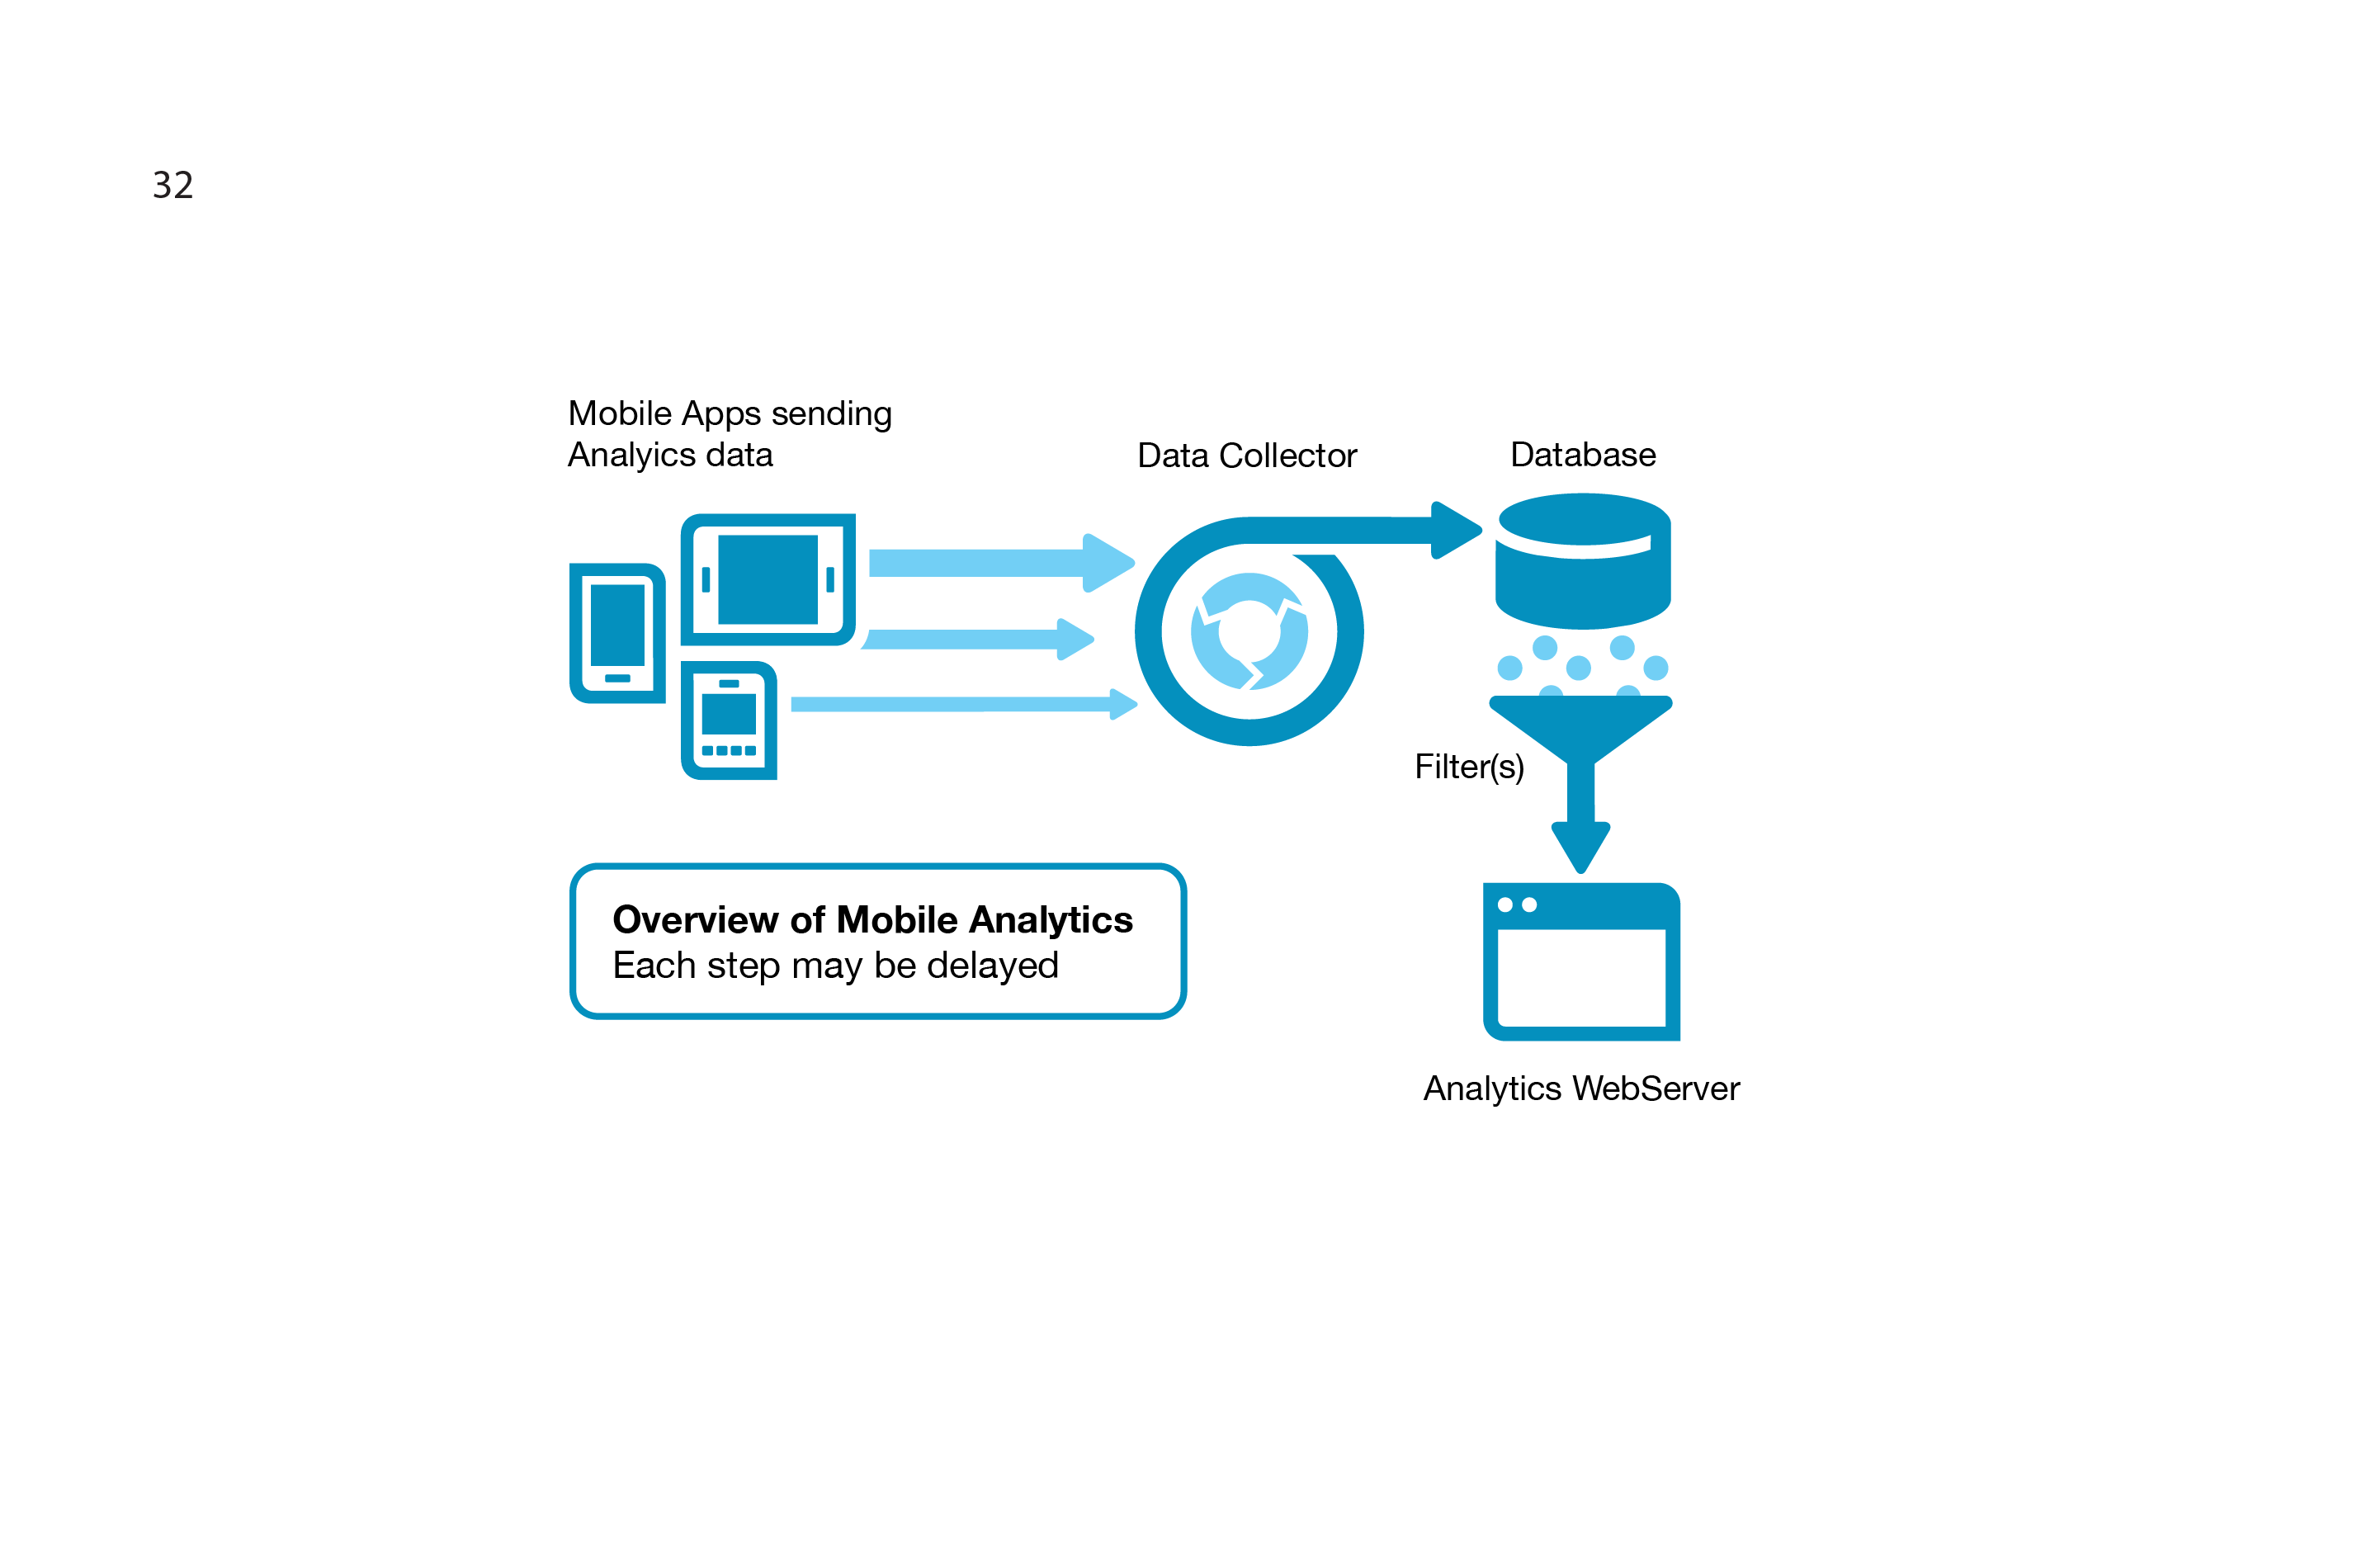
\includegraphics[width=15cm]{images/mobile-analytics-playbook/Chart-08-Overview-of-MobileAnalytics.png}
    \caption{Overview of Mobile Analytics~\citep{harty_aymer_playbook_2016}}
    \label{fig:map2016-overview-of-mobile-analytics}
\end{figure}

An overview of Mobile Analytics was published in The Mobile Analytics Playbook,~\citep{harty_aymer_playbook_2016}, and the figure is reproduced here with permission in Figure~\ref{fig:map2016-overview-of-mobile-analytics}. The overall approach also applies conceptually in terms of how either apps (often delegated to the analytics library implementation) or the device sends the data. As an observation, the approach would also work if the data is transferred using other conduits, such as copying the data using a memory card, however these details are unlikely to apply to the vast majority apps and even for those developers the conceptual model is unlikely to change materially.

Transmission of the contents of the logs and/or mobile analytics data is asynchronous and may occur almost immediately, or in some rare cases months later. In a discussion on the Android implementation of the popular segment.io library, a non-profit reading app needs to store up to six months of reading analytics on the device using this library. The authors discussed practical ways to store the analytics events without loss and then to be able to upload them correctly even where network connectivity is unreliable~\citep{segmentio_supporting_6_months_offline}. Several analytics providers have documented their transmission mechanisms. \emph{``Crashlytics limits logs to 64kB and deletes older log entries when a session's logs go over that limit."} and it~\emph{``...only stores the most recent eight recorded exceptions. If your app throws more than eight exceptions, older exceptions are lost."}.  The non-fatal exceptions are sent the next time the app launches~\citep{firebasecrashlytics2020_customize_crash_reports}. In contrast the Segment implementation for Android stores up to 1000 events~\citep{segment_analytics_for_android_docs}.

One of the particular implementation details may be worth considering, which is the growth in intermediaries and their adoption by developers. Segment provides one such service, where they provide developers with a single per-client app API that then wraps hundreds of potential implementations and offers two \emph{``connection modes"}, device and cloud~\citep{segment_analytics_for_android_docs}. When using their cloud-mode~\emph{``Segment sends messages to the Segment servers, and then translates and forwards that data on to the downstream tools."} Their service becomes a vital additional component in the process and may affect many aspects of the data including privacy, who can analyse it, and latency implications.   

\subsection{Data funnels from users to devs}
The following list itemises a set of possible stages in a data funnel for data that originates from a user's device until it is available for use by the development team. real-world funnels are likely to include a subset of these, in a particular order in terms of the data flow.

\begin{itemize}
    \item Per-app implementation and options
    \item Per-analytics/logging library implementation and options
    \item Farming the log (and/or potentially other usage data) data on device
    \item Device model and operating system combination
    \item Per device implementation and options
    \item Data daemons that control/negotiate what data is and is not available/provided
    \item Data privacy screening (can occur at various points in the funnel)
    \item Batching, queuing, limits, latencies, transmission triggers, ...
    \item Connectivity quality and reliability
    \item Network behaviours e.g. where traffic may be blocked in some geographies, by some network providers, etc.
    \item Data Collector inbound processing (filtering, buffering, validity checks, non-repudiation, dealing with spoofing, fakes, etc.)
    \item Analytics tool filtering and reporting. This may include muting of some aspects of the reporting e.g. for issues considered no longer actionable. 
    \item Content access, storage, combination with other sources, further reporting, etc.
\end{itemize}

Note: there may also be data injected into the funnel, for instance through \href{https://en.wikipedia.org/wiki/Synthetic_monitoring}{synthetic monitoring}, testing of the apps and/or the analytics clients and APIs, spoofing, denials of service, and so on. 

MUST-DO add figure, write up this section.




\section{Conceptual model of usage analytics}
Usage analytics pertains to recording and analysing the usage of software. Application usage analytics is mentioned in various sources, including patents filed by Google in the USA~\emph{e.g.} for methods and systems to collect and provide application usage analytics to developers~\citep{googlepatent_hyman2016_collecting_application_usage_analytics}. 

Conceptually there appear to be four broad levels of usage analytics, these are illustrated in Figure \ref{fig:four-layers-of-analytics-for-mobile-apps} and described next. These four levels can be approximately mapped~\footnote{The approximation is because software is not quite so cleanly cut into layers or levels. For instance app-level mobile analytics can be used to record many aspects of GUI activities, albeit unnaturally. Also, the operating system can observe aspects of the GUI, for instance by instrumenting the Accessibility APIs, a topic I touch on in one of the appendices.} to the three layers of an app:

%\akb{Are 'Visual' analytics tools automatically 'Mobile' tools as well? The \textit{heatmapping} example seems to be one that could fit into both layers}

Their use will be discussed in more detail in the chapter titled~\href{chapter-applying-analytics-to-development-practices}{\emph{\nameref{chapter-applying-analytics-to-development-practices}}}. %MUST-DO decide whether layer and level are synonymous, and if not whether to use one term or the other. Anyway I'm aware I may be conflating both terms here and want to improve the precision of whichever term(s) I use. 

\begin{figure}[htbp!]
    \centering
    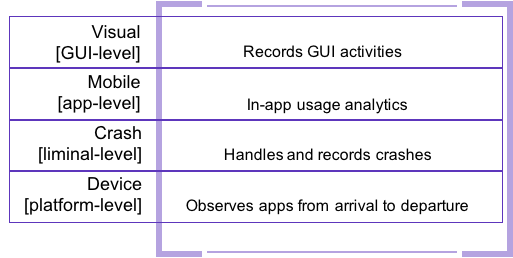
\includegraphics[width=12cm]{images/4-layers-of-analytics.png}
    \caption{Four Layers of Analytics for Mobile Apps}
    \label{fig:four-layers-of-analytics-for-mobile-apps}
\end{figure}

\begin{itemize}
    \item \textbf{Visual (GUI-level)} operates at the GUI level, or layer, of the app. It records aspects of the GUI activities such as touches, gestures, interactions with the screen, and data entry. Often it includes recording what is on the screen too. A common type of Visual analytics is \emph{heatmapping} software. Note: visual analytics may be \emph{implemented} in the app, conceptually they observe the GUI as if from above the UI.
    \item \textbf{Mobile (app-level)} is incorporated as part of the app and records aspects of what the app is doing, in effect aspects of the usage of the app. Mobile Analytics is prevalent in Android apps and already used for various business purposes.
    \item \textbf{Crash (liminal-level)} is where specialised reporting can intercept crashes. Through the interception they can change the behaviour of the app, for instance to provide a better user-experience, log, and report the crash to the developers. \emph{Fatal crashes} are ones where the application quits. These can also be observed by the operating system; for mobile apps the operating system is an intrinsic part of the platform.
    \item \textbf{Device (platform-level)} Platform-level analytics can record apps from when they are installed until they are removed. This recording can include details such as when apps are in-use, crashes, freezes, and so on. Both of the dominant platforms (iOS and Google Android) allow users to decide whether their devices will share this data.
\end{itemize}

% https://new-wine.org/resources/blog/living-liminality-lessons-trust-gratitude-prayer-compassion-global-church-dd508239ff5

This research includes case studies and developer reports of examples of analytic tools that cover three of these four layers of analytics. The remaining layer, visual analytics, is described briefly with a few examples, visual analytics is seldom used in production mobile apps and therefore it was excluded these from the core research. They may be an interesting topic for future research particularly given some of the potential benefits of visual analytics. % COULD_DO add notes on privacy issues and other complicating factors in this sort of research. 

\section{Conceptual model for DevOps}
DevOps recognises the benefits of connecting development and operations of software. a Yin Yang symbol recognises there's some negative in the positive and vice-versa. Conceptually, teams can choose to invest in operations while they're developing to improve the operational aspects of their software, for instance by designing in good operability. Similarly when the software is in use by observing the software's behaviours operations can improve the development. Examples include: considering the how improvements could be developed or the software development lifecycle process improved based on how the software is being used.

\begin{figure}[htbp!]
    \centering
    \includesvg[scale=0.5]{images/wikipedia/Yin_yang.svg}
    \caption{Yin Yang to represent DevOps}
    \label{fig:yinyang_for_devops}
\end{figure}



One of the popular concepts in DevOps is represented by an infinite loop in the shape of a horizontal figure of eight like diagram, illustrated in Figure~\ref{fig:atlassian-state-of-devops-report-2016-devopsloop}.~\footnote{This example is from a blog post by Atlassian~\url{https://www.atlassian.com/blog/devops/2016-state-of-devops-report} announcing \emph{``The State of DevOps report"} 2016 edition.} There are many variations of this illustration available, perhaps unsurprisingly given the popularity of DevOps and those who write and publish on the topic who may want to give their own spin on the topic.

\begin{figure}[htbp!]
    \centering
    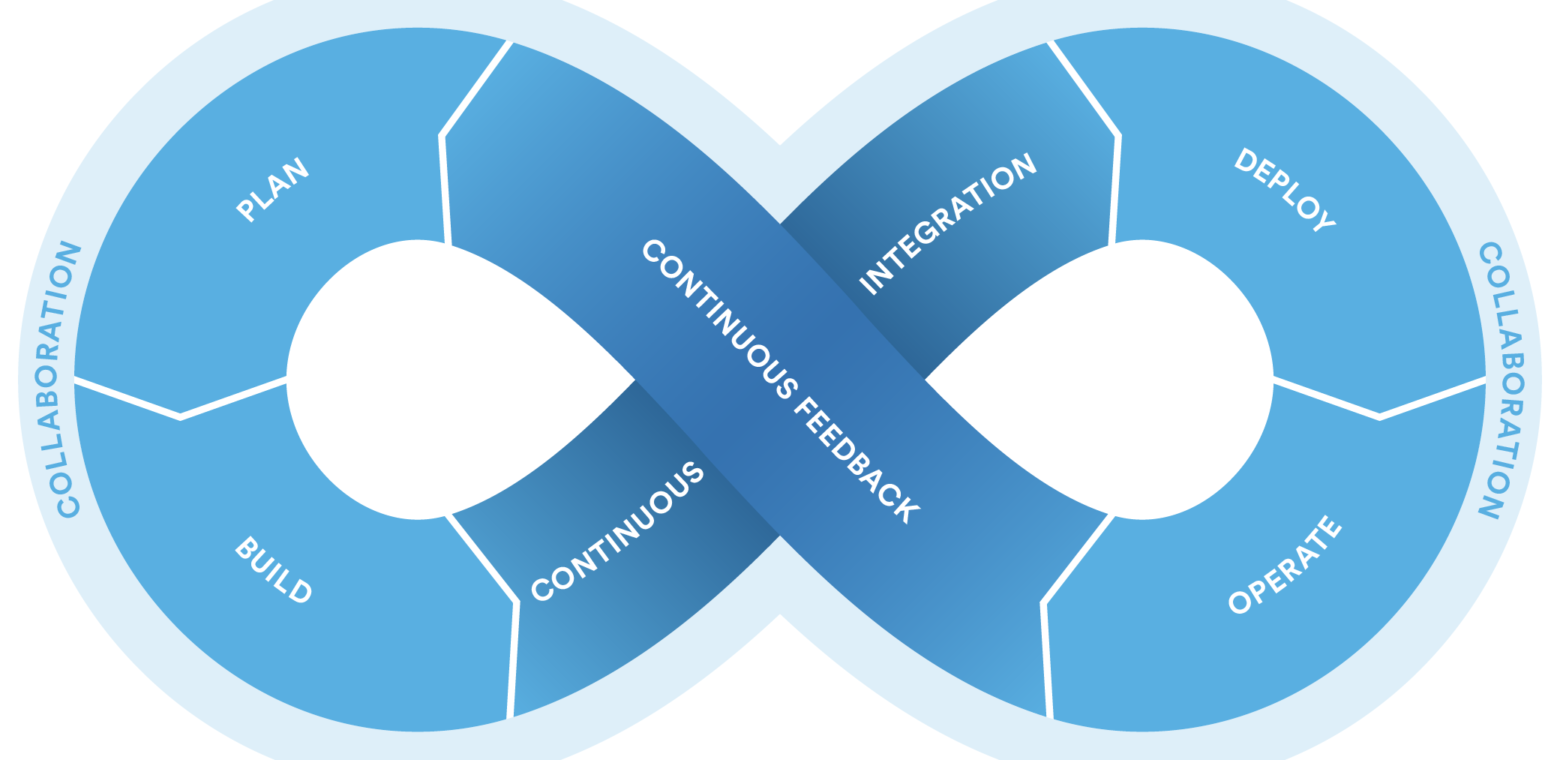
\includegraphics[width=13cm]{images/atlassian/atlassian-state-of-devops-report-2016-devopsloop.png}
    \caption{Atlassian DevOps loop}
    \label{fig:atlassian-state-of-devops-report-2016-devopsloop}
\end{figure}
% https://3kllhk1ibq34qk6sp3bhtox1-wpengine.netdna-ssl.com/wp-content/uploads/devopsloop-1560x760.png



\section{From conceptual models to practicalities}
The previous sections introduced five conceptual models that help to establish the context for the ecosystem, structural aspects of mobile apps and perspectives where mobile apps can be observed, analogue and digital feedback, usage analytics and DevOps considerations. The next five sections cover various practical aspects of mobile apps including development and usage lifecycles, information sources and finally choices for engaging with analytics.

\section{Mobile apps and development team's mobile devices}
A mobile app is more than compiled source code, it includes various resources such as text, images, audio, screen layouts, and sometimes other contents. Many include software libraries from one or more sources. Mobile apps are also digitally signed. Data and information can be obtained for these various constituent parts, for instance some failures may occur within a library at run-time and be reported in logs and via mobile analytics.

Development team's mobile devices, with occasional exceptions are often the same device models that end users have and use; and furthermore they have similar end-user accounts and the majority of their apps are installed in similar ways to those installed on end-user devices. These similarities have some important implications - data on the usage of these devices by the development team may also be collected and considered as being part of the end-user population, and any in-app analytics in the various installed apps may provide their data to the respective mobile analytics systems,~\emph{etc.}

These devices may be configured differently and they may also run local builds and internal releases of apps. The apps may be configured to provide different amounts of information in local logs and/or using mobile analytics libraries for instance to either distinguish the usage or to suppress data from being shared. Knowing and understanding these nuances can help interpret some of the sources of data and information pertaining to these devices and apps.

\section{Mobile app development lifecycle}
To provide some context for this section, Figure \ref{fig:ci-cd-development-and-feedback}~\footnote{Reproduced from \emph{``An empirical study of architecting for continuous delivery and deployment"}~\cite{shahin2019empirical_study_architecting_cd}}
illustrates a modern continuous software lifecycle including feedback. We can observe several distinct stages in the development and deployment of software and the feedback each stage can provide. %MUST-DO check the guidelines for reproducing and citing a figure as-is.
%
In contrast, Figure \ref{fig:google-play-app-development-and-feedback} illustrates a similar software lifecycle for Android apps released through Google Play together with the various forms of feedback~\footnote{Here we have excluded feedback from the app store, nonetheless it exists for many app stores.} 

Key differences between typical CI/CD lifecycles and the one for Google Play is the pre-launch testing and the app store providing both user feedback and a service called Android Vitals. The pre-launch reports are generated automatically by Google where the app store runs automated monkey testing on a farm of Android devices and various static analysis checks of releases deployed to any of the test channels. They are described in~\href{subsection-test-channels}{Test Channels}. %MUST-DO actually add information on the test channels and how releases can be promoted to production releases in Google Play.


\begin{figure}[htbp!]
    \centering
    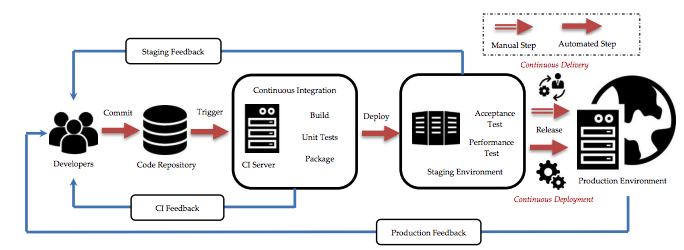
\includegraphics[width=13cm]{images/ci-cd-development-and-feedback.png}
    \caption{CI/CD development and feedback, reproduced from~\cite{shahin2019empirical_study_architecting_cd}}
    \label{fig:ci-cd-development-and-feedback}
\end{figure}

There are additional sources of \emph{analogue feedback} from people, including from alpha and beta testers and end users; and \emph{digital feedback} from Google tools and from usage data collected from the field. These terms are expanded in the section~\href{analogue-and-digital-feedback}{\emph{\nameref{analogue-and-digital-feedback}}}.

\begin{figure}[htbp!]
    \centering
    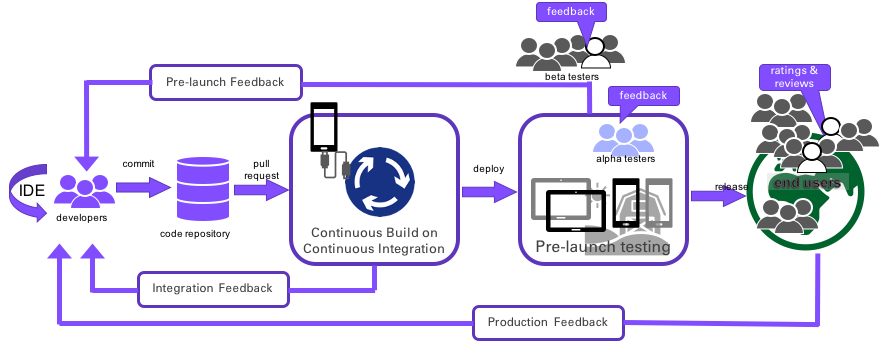
\includegraphics[width=13cm]{images/google-play-app-development.png}
    \caption{Google Play App Development and Feedback}
    \label{fig:google-play-app-development-and-feedback}
\end{figure}

\section{Mobile app usage lifecycle}
Mobile apps have a usage lifecycle, which starts when an app is chosen to be installed and ends with either abandonment or active removal of the app from a device. Figure~\ref{fig:mobile_app_usage_lifecycle}~\footnote{Based on a figure in~\cite{bohmer2011falling_asleep_with_angry_birds}} illustrates the possible stages of a mobile app's life on a user's device. Google Play Console collects data consistent with this lifecycle, analyses it and provides aggregate reports based on their analysis. 

For clarity and completeness there is another lifecycle when the app is running, described in the Android documentation as the \emph{``Processes and Application Lifecycle"}~\cite{android_processes_and_application_lifecycle} These are more detailed and are not included in the reports Google provides developers. %(I doubt their details would be recorded either). 
Note: the processes and application lifecycle may affect how in-app analytics libraries behave, including when they transmit their data to their respective central servers.

% More info and code samples: https://www.vogella.com/tutorials/AndroidLifeCycle/article.html

\begin{figure}[htbp!]
    \centering
    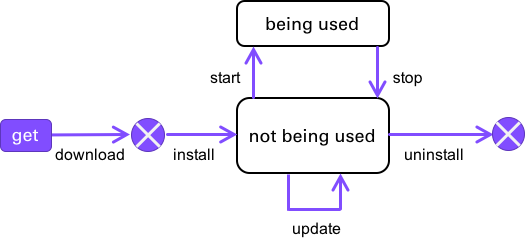
\includegraphics[width=12cm]{images/mobile_app_usage_lifecycle.png}
    \caption{Mobile App Usage Lifecycle}
    \label{fig:mobile_app_usage_lifecycle}
\end{figure}

A later section~\href{platform-level-analytics}{\emph{\nameref{platform-level-analytics}}} provides a proposal of how Google collects the underlying data (they do not document, explain or encourage research in how their system works, We return to their (Google's) reported behaviour and the effects later in this thesis). % MUST-DO add link to: Developers banned from app store ecosystem and their apps removed.
And the chapter \href{appendix-software-contributions}{\emph{\nameref{appendix-software-contributions}}} describes software we developed to help collect data from Google Play Console in order to facilitate both research and to enable developers to collect and use data...

Crashes are often considered a concrete measure of poor performance of software and there has been extensive research in crashes for Android applications, in particular. I suspect there are various reasons for the focus on crashes as an oracle for testing software, crashes are unambiguous (even if the causes are not) and they are also binary so easy to determine whether software has, or has not, crashed. 

In 2017, Google launched a service called Android Vitals as a new, intrinsic part of Google Play Console,~\cite{googblogs_I_O_2017_everything_new_in_the_google_play_console}, where they popularised a measure called \emph{Stability} to assess the quality of Android apps. Their measure includes both crashes and when an application freezes or is unresponsive for at least 5 seconds from a user's perspective, a term Google call Application Not Responding (ANR).


\subsection{DevOps for mobile apps}
This section starts with an overview of DevOps concept of an infinite loop for software generally before becoming more specialised on DevOps for mobile apps. %SHOULD-DO consider expanding this section. TBD how much I should write about the concepts and terms. 
The focus here is on data from various stages of a conceptual infinite combined development and operations process to indicate where mobile analytics applies in terms of providing data to the development team. This data includes: log data, static analysis results, test results, release and usage data, and mobile analytics data and reports.

In October 2020, one of the students taking part in the PhD symposium at the ICST2020 conference presented a variation of the DevOps loop (as illustrated earlier in this chapter in Figure~\ref{fig:atlassian-state-of-devops-report-2016-devopsloop}) that is relevant to this research. In the student's figure their focus was on crash reproduction and this illustration is temporarily illustrated in Figure~\ref{fig:crash-reproduction-icst2020}(~\emph{pending an update from the presenter of that topic}).

\begin{figure}[htbp!]
    \centering
    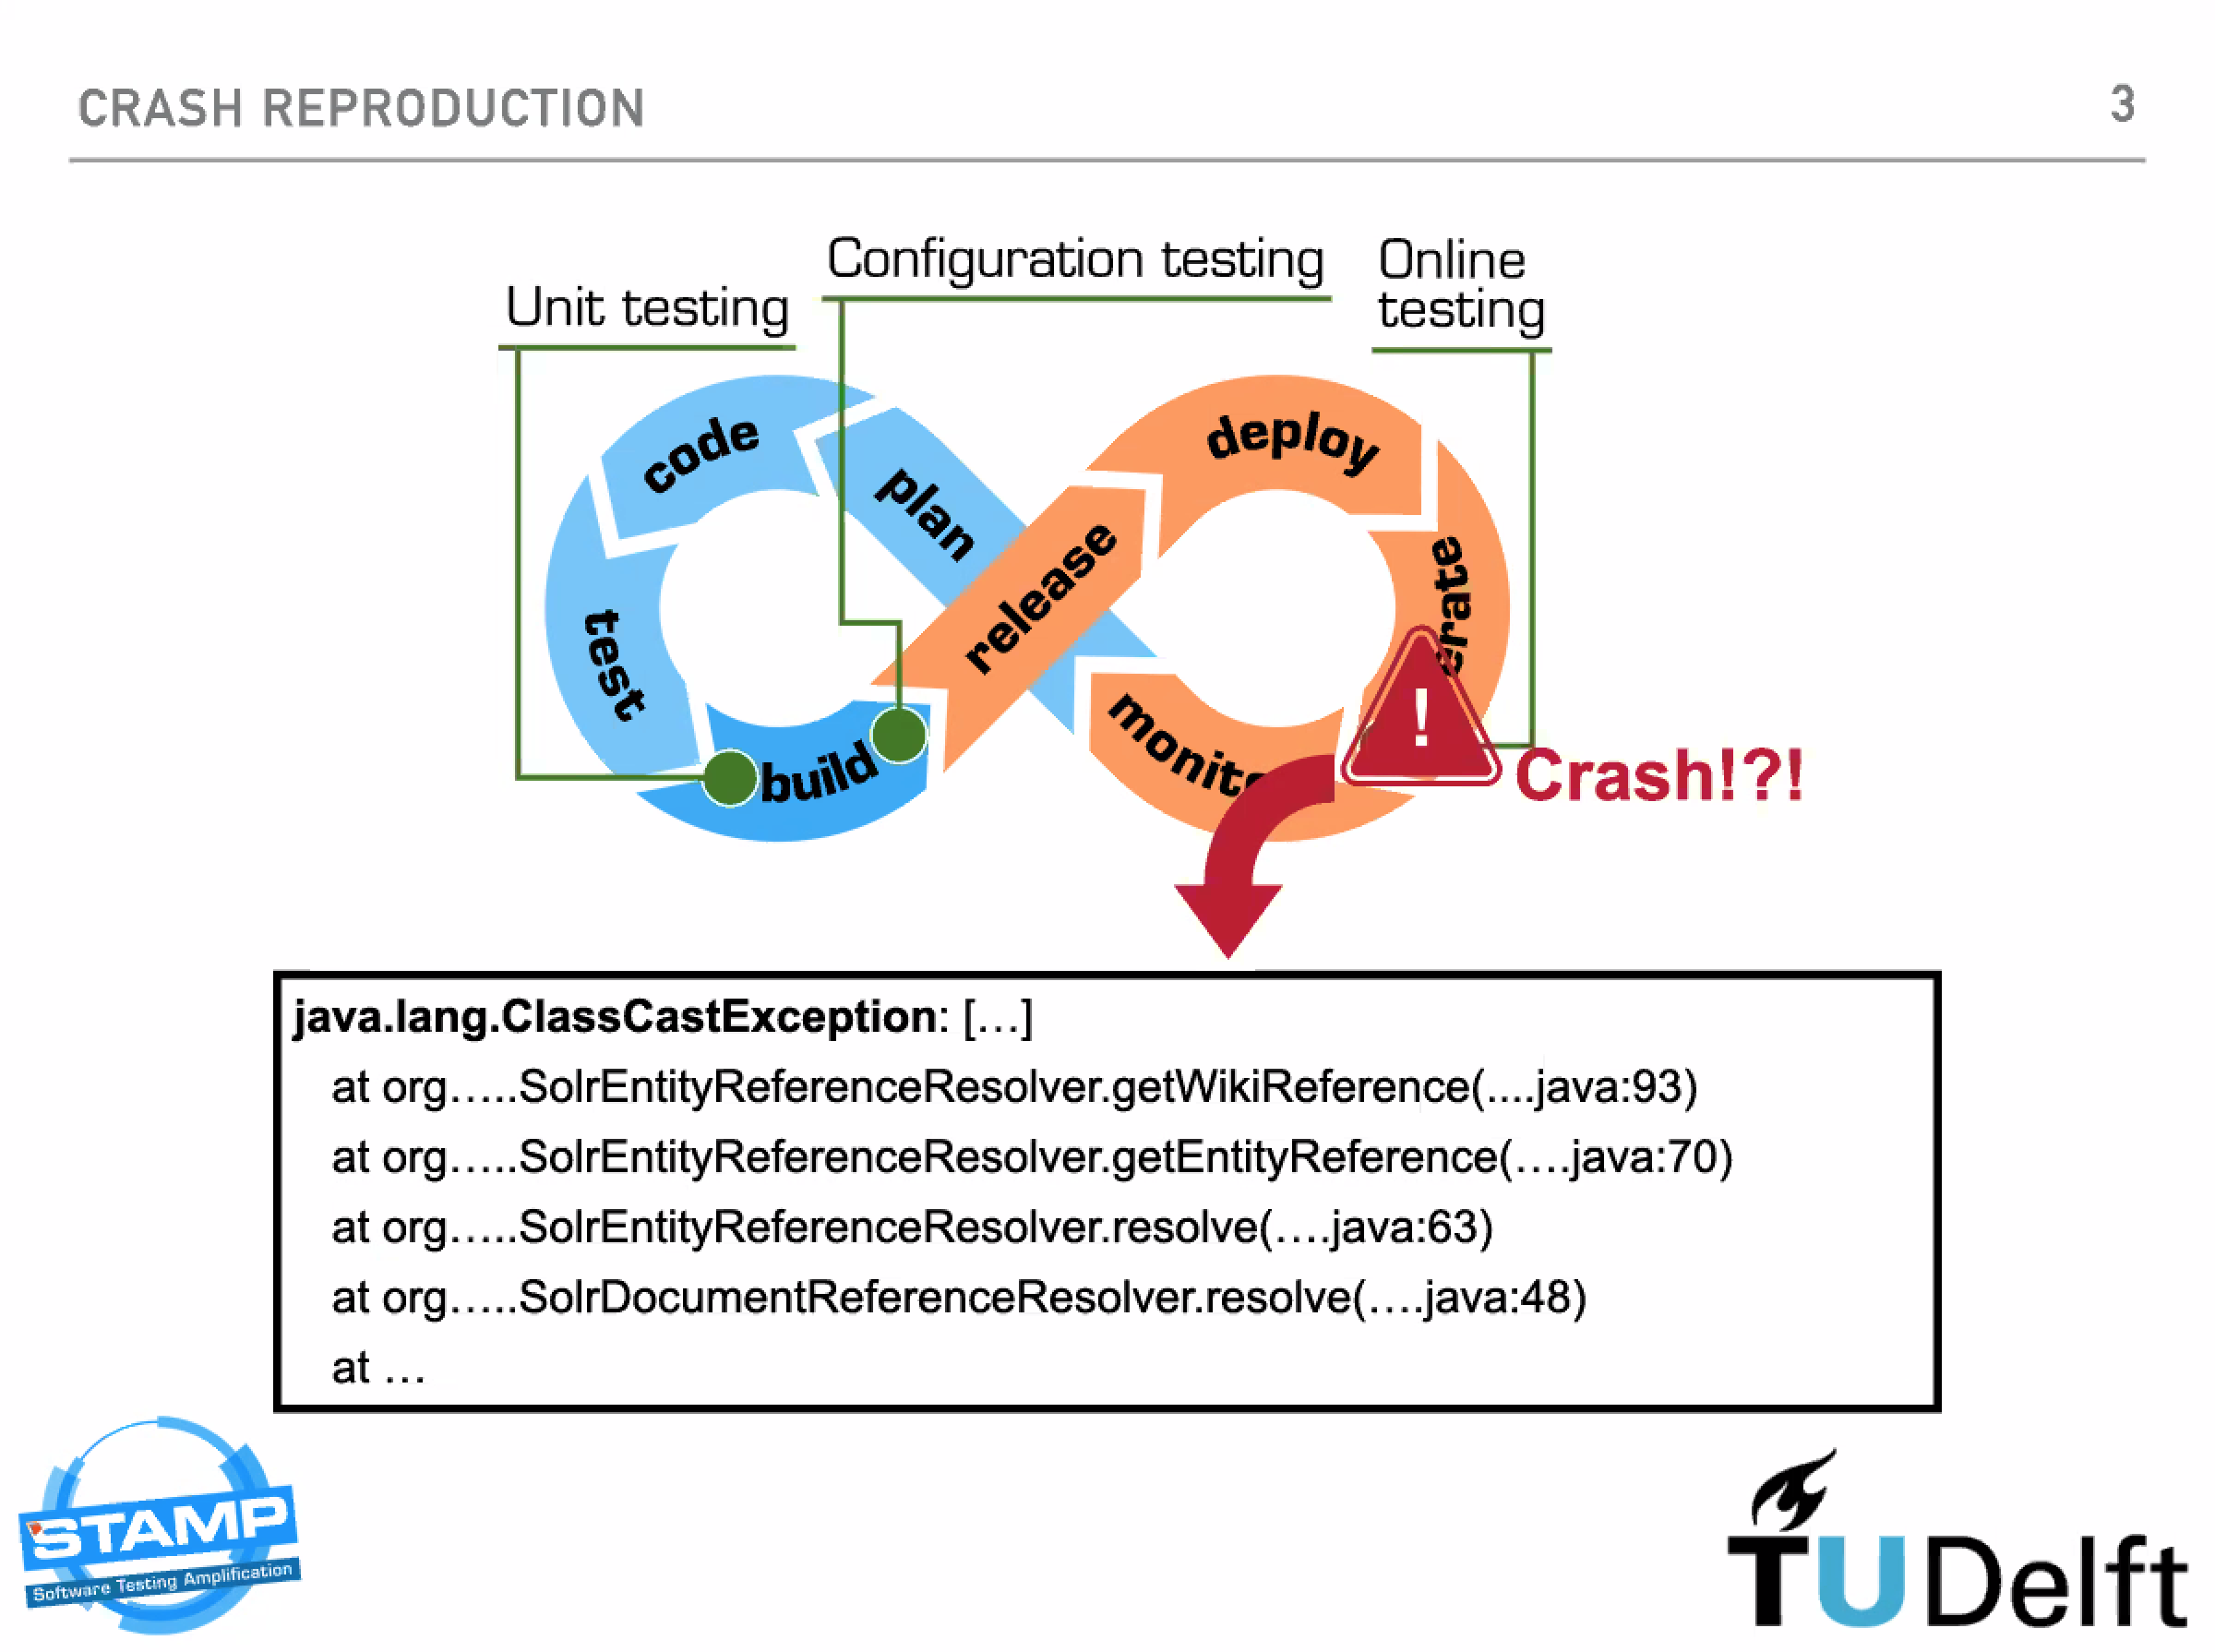
\includegraphics[width=14cm]{images/icst-2020/crash-reproduction-icst2020.png}
    \caption{Temporary image: Crash Reproduction}
    \label{fig:crash-reproduction-icst2020}
\end{figure}

Figure~\ref{fig:oberve-and-apply-devops-loop} is revised illustration that shows, in red, the extent software can be observed, and in green of when the results of those observations can be applied to the code. Note: the observations can be applied throughout every phase, for instance during deployment aberrant behaviour observed during the deployment may lead to the deployment being paused.

\begin{figure}[htbp!]
    \centering
    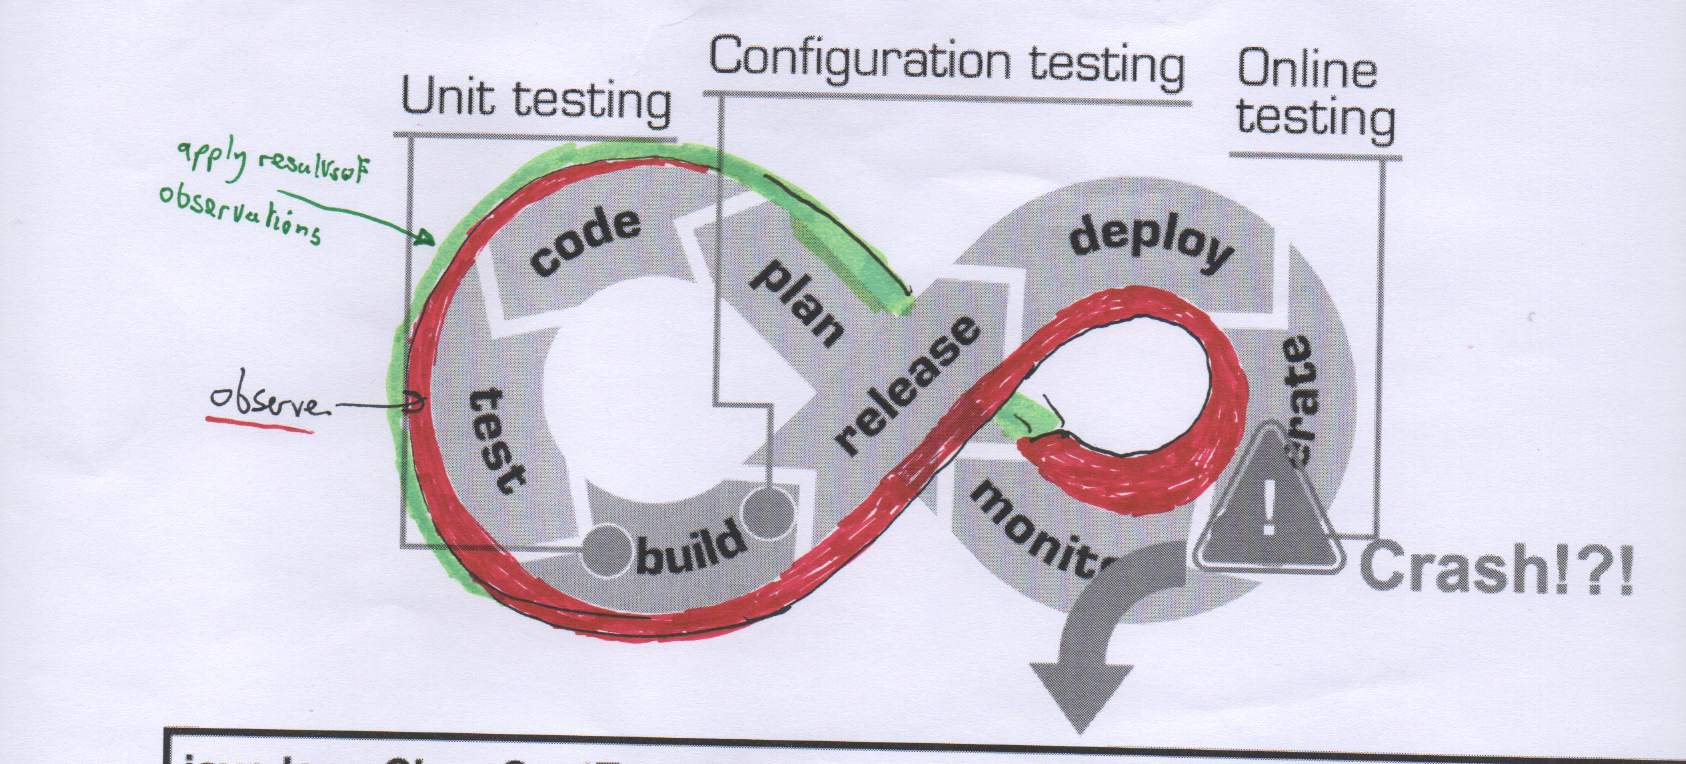
\includegraphics[width=14cm]{images/rough-sketches/hack-of-devops-crash-figure.png}
    \caption{Rough Sketch: Concept of feedback on software and applying it}
    \label{fig:oberve-and-apply-devops-loop}
\end{figure}

Data is available using various sources about software from the outset of coding until the software dies; however for the purposes of this thesis the focus is on when the software is actively used and maintained, as illustrated in the previous three figures:~\ref{fig:atlassian-state-of-devops-report-2016-devopsloop},~\ref{fig:crash-reproduction-icst2020},~\ref{fig:oberve-and-apply-devops-loop}. 

During coding code analysis tools such as static analysis identifies patterns of potential concern in the source code and similar artifacts such as GUI layouts, strings in resource files, and so so. Tests can also be created and performed from the outset of the coding to provide runtime feedback (~\emph{i.e.} data) about the software under test, and similarly developers can add logging statements and also use logging built into the operating system that both provide data that can be mined to learn about the software's behaviours.

The build process may include configuration details, for instance to create a range of custom applications, to include instrumentation, to compress and obfuscate the application binary, and to create debug and release editions of the software. Data about the build process and about what has been built may also be observed and analysed and the products tested and analysed; for example an application binary can be scanned for information leakage in an obfuscated build, and builds can be tested to provide more data about how the software performs.

The release and deployment phases will be covered in more detail in the next section; here the focus is on the data available as part of these phases. 

As software is released the software transitions from being within the view of the development team to being used by others where the development team no longer has direct access to the devices that have the app installed or being used. They are remote from the use of the app. This means that local access to devices (to see what's happening and to try things out) and to the device's logs are unlikely to be practical, other sources of information now need to take precedence.

The release of a mobile app using an app store is subject to the processes and controls applied by the provider of the app store. The app store may offer both free and paid-for optional services to the developer, for example Google provides optional, free pre-launch reports that contain the results of automated testing and static analysis of application binaries. The app store may provide reports to the development team particularly if they decide to delay or block a release or suspend an app from being downloaded by end-users.

Usage is the ultimate active phase for a mobile app installed on a user's device. Simplifying slightly, as some apps run automatically in the background, most apps are started and used by end-users. Aspects of the usage can be recorded by various software utilities, in particular by the platform which records when an app starts and when it terminates. The platform can also record when an app is installed, when it is updated, and when it is uninstalled. The app store may provide developers with reports and statistics on the app's install base and usage. The app store may also provide developers with information about the performance of the app including any failures of the app while it was running.

Crashes are logged locally by the platform, some platforms may also record other failures and performance related data as well as resource utilisation and various capacities such as battery level locally. The platform may have permission from end-users to forward a copy of the information logged locally on the device and to use it for various purposes.  

\subsection{Software releases for mobile apps}
For mobile apps, the release management may include deployment of the app to end-user's devices either as a fresh install for new users or as an update for existing users that app on a given device~\footnote{Mobile apps for Apple and Google app stores are installed per device and licensed per user so users can freely choose how many devices to install an app on, and they may even have different releases of the same app on different devices.}.

Releases may be acute or chronic in nature. Acute releases are actioned immediately and deployed as soon as practical. Chronic releases may involve alpha (closed-group membership) and beta (open-group membership) testing followed by rollout in stages, for instance starting at 10\% of the user-base, then increasing to 25\%, and so on until the new release is available to 100\% of the user-base. Note: there is no guarantee that the new release will be deployed to the entire user-base, and in my experience some users will keep using much older releases for as long as several years after newer releases were made available to them. 

The actual deployment and market penetration of a new release depends on several factors which may be outside the developer's direct control. This particularly applies for mobile apps made available through an app store where the app store and end-users can block new releases being applied. In my experience across a range of Android apps, for a 100\% rollouts it takes about a week for the new release to be installed on 50\% of the user-base's devices, however the range varies from 3 days to several weeks to reach 50\%.  

\begin{figure}[htbp!]
    \centering
    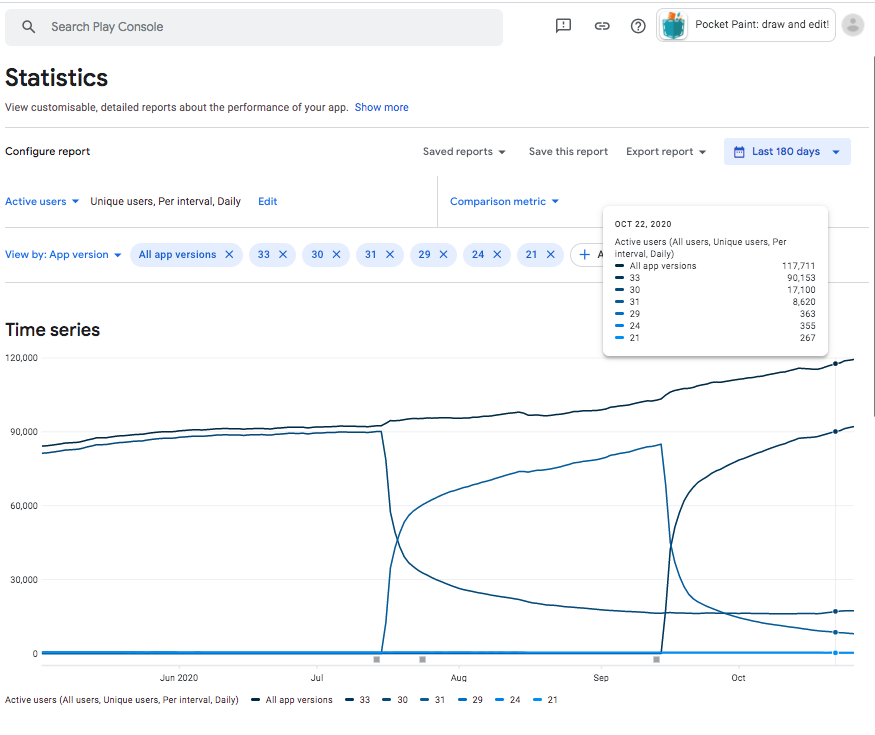
\includegraphics[width=15.5cm]{images/android-vitals-screenshots/PocketPaint-ActiveUsers-180days-2020-10-29.png}
    \caption{PocketPaint Active Users 180 days by app version}
    \label{fig:pocketpaint-180d-active-users}
\end{figure}

Figure~\ref{fig:pocketpaint-180d-active-users} illustrates a typical pattern of the majority of the userbase migrating from one app release to another and yet others remain with older releases during this period of 180 days (apologies for the small text in the image it was impractical to resize it adequately). Note: Google defines active users as:~\emph{``
The number of users who have your app installed on at least 1 device that has been turned on in the last 30 days"}~\footnote{Text extracted from the online help for the `Active users' contextual help icon in Figure~\ref{fig:pocketpaint-180d-active-users}.} so it's not necessarily those who use the app in this period. The residues of users who remain on older releases of the app constrains the rate of change of the overall statistics as measured by Google Play Console and Android Vitals. This means that old buggy releases may continue to adversely affect the overall stability metrics for the app for long periods, even for months and years. Conversely, the project team may have addressed some of the causes of poor stability yet don't have a viable way of proposing users upgrade to the newer releases, and sometimes newer releases may have undesirable features or characteristics from an end user's perspective.

\begin{figure}
    \centering
    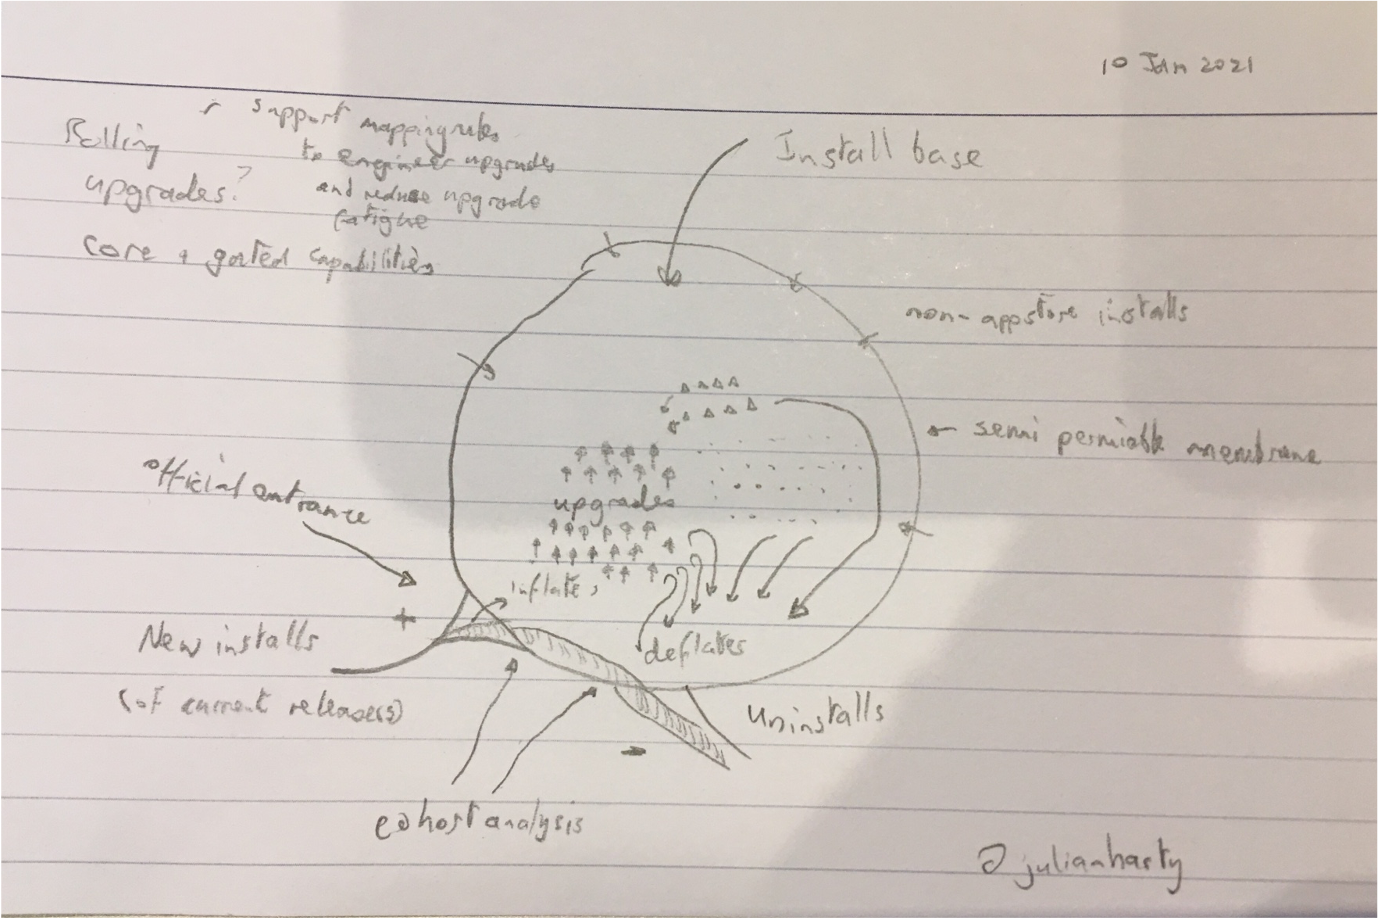
\includegraphics[width=14cm]{images/rough-sketches/app-install-base.png}
    \caption{App install base}
    \label{fig:app-install-base-rough}
\end{figure}

\textbf{Installation base}: The rough sketch in Figure~\ref{fig:app-install-base-rough} illustrates static and dynamic aspects of the installation base for a mobile app. The approximate circle contains the installation base for an app. The size ebbs and flows based on new installs - which inflate the shape, and uninstalls - which deflate it. In current mainstream app stores users do not get a choice of which release of an app they will receive when they receive it, that choice is made by the app store using one or more releases provided by the developer. The app store may allow developers to choose various criteria for current releases, such as a percentage rollout, and then apply that on behalf of the developer. The boundary may be considered semi-permeable as some installations are not sourced from the app store. A key consideration is that upgrades apply to the install base so they occur within a population and do not change the number of installs. That said they may lead to decreases in the installation base for various reasons. Some users may uninstall an app prompted by learning of a new update of the app - for instance if it requires permissions the user considers intrusive or unsafe; others may uninstall the app after the update, for instance if they believe it is too buggy to merit using. Note: they are not able to revert to an earlier release within the current major app store's practices / constraints. 

To sum up so far, new installs receive the most current release gated by the rollout algorithms implemented by and in the app store. Upgrades also receive the most current release gated by the same rollout algorithms.

\textbf{Cohorts}: represent a group of users who share something in common and measures at intervals through time. Examples include new users who install the app on a particular day or in a particular week. They are used in analysis, for instance to measure what proportion of new users still have the app installed a week later. Cohorts can also be used to group users with a distinct release of an app, and so on. Useful introductions to cohort analysis using Google Analytics are available online~\citep{codehouse2020_cohort_analysis, googleanalytics2021_the_cohort_analysis_report}, and cohorts are used in various analytics tools including Google Analytics and Firebase Analytics. 

% https://www.codehousegroup.com/insight-and-inspiration/digital-strategy/cohort-analysis-and-how-to-use-it-in-google-analytics
% CHEST journal: Cohort Studies https://doi.org/10.1016/j.chest.2020.03.014

One reason why users uninstall an app is because of poor quality behaviours by the app. In a survey by Dimensional Research, 3011 participants completed an electronic survey to identify key factors that led to end user satisfaction with mobile apps. The research also `... sought to determine what users did when they were unsatisfied with a mobile app.' (page 5). 
53\% of respondents have uninstalled or removed mobile apps that regularly crashed, stopped responding or had errors and 37\% stopped using the app (page 16)~\citep{dimensionalresearch2015_mobile_app_use_and_abandonment}~\footnote{The report is free of charge upon request: \url{https://techbeacon.com/resources/survey-mobile-app-users-report-failing-meet-user-expectations}}.

To sum up again, the installation base relies on a combination of existing and new users. Updates can lead to some existing users uninstalling the app - a topic to consider when planning releases of the app. Cohorts can be used to measure the effects of new releases of an app and several analytics tools already use them for tracking the retention of new users. Poor quality of an app may lead to more uses abandoning and even uninstalling the app. As a hypothesis: if an update of an app improves the quality of an app for a user the user may be pleased with the update and continue using the app, conversely if an update does not improve the quality of the app for that user some users will merely stop using the app others will actively deinstall it. Releases can be a point of inflection in terms of the userbase.

\textbf{Forced updates?} Some developers, and some platforms, may incorporate mechanisms to encourage or even try to force users to update their apps. However, doing so may upset and alienate some users. One of the case studies,~\href{section-greentech-apps}{\emph{\nameref{section-greentech-apps}}}, has used these mechanisms and this topic will be expanded in that case study. In contrast, the Kiwix Android app has over 70 releases being reported as active in a 7 day period, some several years old. Figure~\ref{fig:kiwix-30d-active-users} shows the overall active user base and the top ten of the 70+ releases according to Google Play Console~\footnote{Google Play Console limits the graph to ten items on the secondary category.}.

\begin{figure}[htbp!]
    \centering
    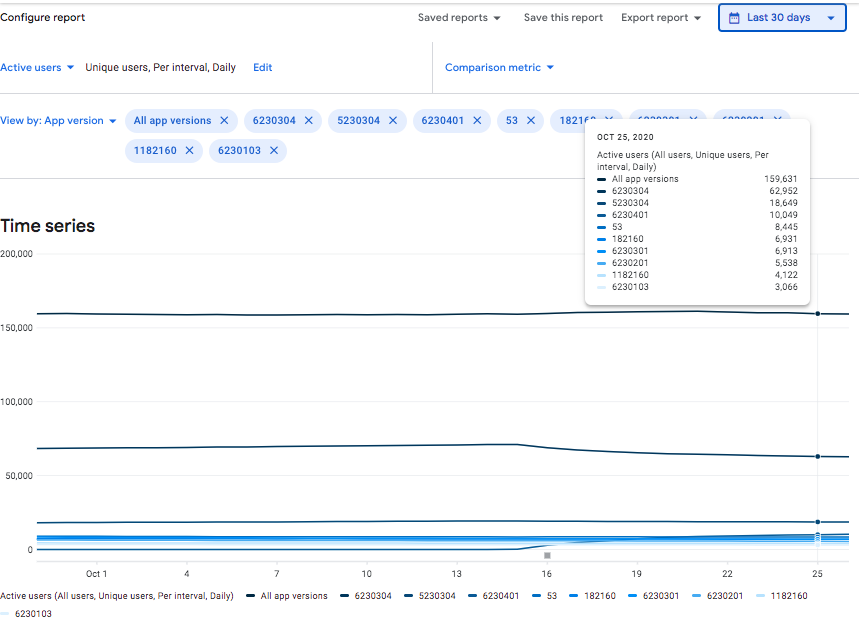
\includegraphics[width=15.5cm]{images/android-vitals-screenshots/kiwix-ActiveUsers-30-days-2020-10-29.png}
    \caption{Kiwix Android Active Users 30 days by app version}
    \label{fig:kiwix-30d-active-users}
\end{figure}

As mentioned above, there are various practical constraints to the frequency of releasing mobile apps using an app store. Chiefly there are two constraints: 1) the relatively slow rollout of new releases to the user-base which can take a week or more to achieve 50\% and also 2) the app store's review process which has been a hotly debated topic particularly by developers who may end up waiting days or even weeks for a release to be approved. Apple states~\emph{``Review times may vary by app. On average, 50\% of apps are reviewed in 24 hours and over 90\% are reviewed in 48 hours."} and Google informs developers in Google Play Console~\emph{``We're experiencing longer than usual review times
Due to adjusted work schedules at this time, you may experience longer than usual review times for your app."} ~\footnote{This message is on the \texttt{app-dashboard} page for each app in Google Play Console and only visible to authorised development team members}. Sophisticated development teams may find ways to alleviate these constraints, for instance by shipping code updates that are applied by a current release rather than by creating and releasing a new binary of the entire app.

Given the constraints that are faced by the vast majority of mobile app developers, of rollouts taking many days and of needing to cope with sometimes lengthy delays in app approvals. 

Mention poor behaviour and their effects on app approvals.

TODO Discuss limits on releasing often that lead to an adapted set of working practices, release frequencies, etc. Perhaps do so elsewhere in this thesis?


\section{Information sources for app developers}
Developers want and need to know how well their apps are performing from various perspectives such as: growth and adoption (\emph{``do we have more users and are they using the app [more] often?"}), users' ratings and reviews (\emph{``do they like our work?"} and in terms of quality (\emph{``does it perform well? is it fast and reliable?"}). 

\begin{figure}[htbp!]
    \centering
    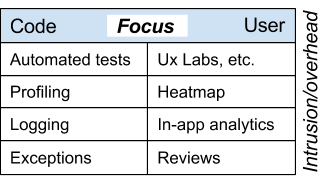
\includegraphics{images/ComparingTechniquesRHS.png}
    \caption{Comparing Techniques}
    \label{fig:comparing_techniques}
\end{figure}

\begin{table}[htbp!]
    \parbox{.40\linewidth}{
        \centering
        \small
        \begin{tabular}{lll}
            Technique  & Gen. Effort & Usage Effort  \\
            \hline
            Automated Tests  & High  & Medium \\ 
            Profiling   & 1 & 1 \\
            Code Quality tools & 1 & 1 \\
            Logging   & 1 & 1 \\ 
            Exceptions  & 1 & 1 \\ 

        \end{tabular}
        \caption{Focus: Code \label{HRVtable}}
    }
    \hfill
    \parbox{.40\linewidth}{
        \centering
        \small
        \begin{tabular}{ll}
            Technique & vector$_1$  \\
            \hline
            UX labs, etc. & 1  \\ 
            Heatmap & 1  \\ 
            In-app feedback & 1  \\ 
            App-store reviews & 1  \\
        \end{tabular}
        \caption{Focus: User \label{BACtable}}}
    \caption{Comparing techniques}
\end{table}

HRV data in Table \ref{HRVtable} and BAC data in Table \ref{BACtable}.

There are various techniques that can be used to assess aspects of quality of mobile apps. Figure \ref{fig:comparing_techniques} provides a visual overview of eight techniques. Of these four are code-oriented and the remaining four more user- or usage- oriented. They are ordered in approximate rank of the overhead, effort, or intrusion involved of each technique. % MUST-DO continue and expand this argument. Discuss why exceptions were chosen as one of the core elements of this research and PhD thesis.

Google's Google Play app store provides developers with answers to all these niggling questions through a developer-oriented user interface called Google Play Console. 
In Google Play Console they provide various tools, reports and data all aimed at informing developers about how their apps are 'doing' and performing. Broadly, these include an overview page with one line of pre-selected data per app managed by the Google Play \textit{Developer Account}. Then, per app, Google provides an overview dashboard of graphs which, in turn, link to more detailed reports and information which provide greater depth. (Examples are provided in the~\href{appendix-analytics-tools}{\emph{\nameref{appendix-analytics-tools}}} appendix.)  Some graphs only appear when Google's algorithms decide they are relevant, these seem to be related to events and/or volumes of underlying data.




\section{Passive, tacit, and explicit analytics choices}
Various degrees of choices are available depending on how actively the development team wishes to incorporate analytics into their development practices. These include using what already exists, where the data is gathered by others and made available to the developers, here these sources are called \emph{passive analytics}. Developers can choose to take more authority in the data collection, for instance by deciding what data they would like to collect and how they wish to collect it. They can use these tools at various depths, ranging from superficial use to actively maximising the efficacy of using analytics to provide them with the data they believe they need to achieve their outcomes. There is an interesting discussion in a blog article~\cite{mukherjee_implicit_versus_explicit_event_tracking_hits_and_misses} on what they term \emph{implicit, or codeless} and \emph{explicit or code-based} event tracking using web analytics tools. The article compares the benefits (hits) and flaws (misses) of both approaches. It also provides a flow chart to help teams select analytics tools that suit their context.

% More reading
% https://web.archive.org/web/20120401053907/http://www.wiikno.com/blog/explicit-vs-implicit-data
% MUST-DO check Patrick's recording of this webinar: https://snowplowanalytics.com/events/explicit-vs-implicit-tracking/ and write up germane items here.


\subsection{Passive Analytics}~\label{subsection-passive-analytics}
Passive analytics are those not actively under the control or influence of the development team, they are provided from other sources such as the operating system or the app store. In the context of this research the passive analytics are all managed by the app store, Google Play, and made available to developers through Google Play Console. As Google states in a US patent,~\emph{``several services provide passive analytics collection such as receiving information about the device type, time of usage, location usage, feature usage, and event reporting."}~\cite{googlepatent_hyman2016_collecting_application_usage_analytics}.  

% COULD-DO compare with the concept of passive monitoring https://en.wikipedia.org/wiki/Passive_monitoring however the Wikipedia article doesn't currently add enough to justify citing it or comparing with it.

\subsection{Tacit Analytics}~\label{subsection-tacit-analytics}
Tacit is variously defined as \emph{``Something tacit is implied or understood without question."}~\footnote{\url{https://www.vocabulary.com/dictionary/tacit}}, \emph{``Understood or implied without being stated."}~\footnote{\url{https://www.lexico.com/en/definition/tacit}, Note: Lexico.com is a new collaboration between Dictionary.com and Oxford University Press~\url{https://www.lexico.com/about}}, silent, wordless, or noiseless. 
%
It may be something that is inherent in the nature of using many of the third-party analytics libraries. In this research~\emph{tacit analytics} is where developers accept whatever default data is collected by an analytics library without the developer needing to do anything more than integrate the library into their app. 

\subsection{Explicit Analytics}~\label{subsection-explicit-analytics}
Explicit analytics is where developers have actively added code to interact with analytics libraries, for instance by calling methods in the API(s) provided by the library's. There are various degrees of use of the APIs and developers may have various intentions for calling these APIs.

\section{Drilling down into analytics}\label{section-drilling-down-into-analytics}
At the highest level of information, an item and an associated number provides some information: a total crash rate of 99.1 \%, 97K total installs, 37 reviews, and so on. These values may change over time, however if we do not keep track of previous values they cannot be compared, and also relevant information may be hidden behind the totals. The total sums up as many values as exist (from zero values onwards). Some of the reported analytics are of this high-level form.

Totals for subsets of the overall volume of data helps provide additional and potentially relevant information. Relevant subsets for mobile analytics include: date ranges, app releases, platform versions, and many others. Other examples, found in some analytics tools include crash clusters - collections of crash reports considered to be sufficiently similar to enable various individual crashes to be grouped and aggregated. The ability to segment and report on segments allows more detailed analysis than simply observing subsets. 

Comparisons with one or more peer groups provide relational analytics, helping answer: ``how is this app performing compared to various peer groups?" Unless the team has direct access to the data for their peer group, the statistics for the peer group need to be available to a trusted party who perform the comparisons. Some data is publicly available for instance the overall rating of an app together with a limited number of recent reviews and the total installs \textbf{MUST-DO} write up research that uses these sources in the related works chapter, add some of the citations here. There are also commercial services available, and some analytics tools, including Google Play Console, provide these comparisons as part of their services.

Individual records provide the most detail that's available. Note: Developers may be able to create new records and enhance existing records and/or add additional forms of analytics if they want/need more detail. Examples of individual records include stack traces for crashes and similar internal state data for ANRs. Some analytics tools allow developers to capture and subsequently see individual records, for instance details of an item added to an e-commerce shopping cart by an end user. Mobile analytics ultimately can only report on data that is provided to it. 

The analytics tool may or may not make aspects of the data available to the users of the tool. As a concrete example, Google Play Console provides developers access to individual reviews (with their associated rating), it also used to provide access to crashes and ANRs for several years before removing these and replacing them with summary data in 2018 \textbf{MUST-DO} add reference and cite it.

\textbf{MUST-DO} provide screenshots of category peer groups and custom peer groups. Discuss either here, or in a later chapter, Google's cap on the number of changes to the custom peer group.

Two key points in summary: being able to keep track of analytics as they change over time allows comparisons and trends to be determined. Additional detail can help identify meaningful differences for instance that a crash rate is much higher than the mean for a particular model of smartphone. 

How much information is needed to be actionable? (Thought: This may be more of a research question...)


\textbf{MUST-DO} introduce my concept of resolution.

\textbf{PERHAPS} introduce the concept of app peer groups here?


\section{Summary and transition}
% This chapter has introduced various concepts and topics which help provide context for the rest of this thesis. Some additional background material is available in various appendices, including more information on mobile analytics and various software contributions.
We now have a grounding in the domain of mobile apps, logging and mobile analytics which is underpinned by research in both academic research and grey literature. The next chapter describes the application of mobile analytics to software development practices for mobile apps.

%\chapter{Evaluation}
This chapter evaluates the research performed during the PhD.

The case studies both led to significant improvements to the measured reliability of the treatment app. 

For the Kiwix project this reduction was one of the main reasons why they then chose to update the codebase for the majority of their custom apps~\footnote{The Kiwix project team decided some seldom used apps were not worth updating.}. They achieved similar improvements in the measured reliability despite only using the default analytics provided by Google Play Console. 

For the Catrobat project the development teams chose to add crash and mobile analytics to their iOS app which had neither previously and mobile analytics to their Android app, as it already incorporated crash analytics.

\section{Evaluation of the Kiwix case study}
%%%% Table generated originally by Spread-LaTeX
%\begin{adjustwidth}{-1 cm}{-1 cm}
\begin{threeparttable}[!htp]\centering
\caption{Reductions in Crash Rates}\label{tab:evaluation-reductions-in-crash-rates}
\scriptsize
\begin{tabularx}\textwidth{lrrr} % SHOULD-DO I'd like to reduce the width slightly.
\toprule
%& & & & \\
&\multicolumn{3}{c}{30-day crash rates reported in Android Vitals~\tnote{0}} \\
\midrule
\multirow{2}{*}{.} &\multicolumn{2}{c}{Kiwix Apps} \\
Stage &Release&\cellcolor[HTML]{efefef}Experiment &Control  \\

&\cellcolor[HTML]{efefef}&\cellcolor[HTML]{efefef}Kiwix & WikiMed English \\

1 &0 
  &\cellcolor[HTML]{efefef}5.07\% &1.13\% \\
2 &1 &\cellcolor[HTML]{efefef}3.12\%~\tnote{1} &\multirow{2}{*}{\cellcolor[HTML]{A8A8A8}}... \\
3 &2~\tnote{2} &\cellcolor[HTML]{efefef}1.59\%~\tnote{3} & \cellcolor[HTML]{A8A8A8}... \\
  &3 &\cellcolor[HTML]{efefef}0.53\%~\tnote{4} &1.09\%~\tnote{5} \\
4 &4 &\cellcolor[HTML]{efefef}0.72\%~\tnote{6} &0.60\%~\tnote{7} \\
  &4~\tnote{8} 
&\cellcolor[HTML]{efefef}0.55\% &0.41\% \\
  &5 &\cellcolor[HTML]{efefef}0.40\%~\tnote{9} &0.26\%~\tnote{10} \\
\bottomrule
\end{tabularx}
\begin{tablenotes}
  \item[0] Except when otherwise noted.
  \item[1] Kiwix Release 2.5 with the previous custom download facility replaced by a Google Android downloader.
  \item[2] The code is under 25 lines including 10 lines of comments~\url{https://github.com/kiwix/kiwix-android/pull/1388}.
  \item[3] Aggregate crash rate over 7 days for versions 2.4, 2.5.1, 2.5.2, 2.5.3 (to Aug \nth{26} 2019).
  \item[4] Previous 30 days crash rate, before release 3.1.2 pushed the crash rate up (same graph as TODO).
  \item[5] \emph{Unchanged release from the first control.}
  \item[6] Includes 3.1.2 which had an average (mean) crash rate of roughly 1.7\% (roughly \nth{31} Dec 2019).
  \item[7] A mixed set of crash rates, averaged by Android Vitals. For the first updated release of Wikimed (the 2019-12 release).
  \item[8] As usage increased of the more reliable releases the averages declined.
  \item[9] The crash rates for releases 3.2.1 are 0.23\% and 3.3.1 are 0.31\%
  \item[10] Release 2020-03 actually has a crash rate of around 0.05\% the numbers are higher as there are still significant volumes of usage on the previous 2 releases.

\end{tablenotes}
\end{threeparttable}
%\end{adjustwidth}
\vspace{5mm}
%%%% Isabel recommends creating a timeline instead - sounds good SHOULD-DO

Table~\ref{tab:evaluation-reductions-in-crash-rates} provides a numerical summary of five releases of two of the Kiwix Android apps. There are four stages in this case study:

\begin{enumerate}
    \itemsep0em
    \item The baseline
    \item Simplifying the most buggy code
    \item Applying the concepts in the research to the experiment
    \item The new normal: %ongoing improvements to the experiment app \emph{and} applying these improvements to the custom apps (including the previous control app).
\end{enumerate}
% Great ideas to reduce space in list items in https://tex.stackexchange.com/questions/6081/reduce-space-between-enumerated-items
% COULD-DO I've only applied the basic suggestion for this single list so far, might be worth thesis wide changes as the thesis matures.

The active part of the experiment started in stage 3 of this case study, although the initial research into the feasibility started several months earlier during the baseline stage.

\subsection{Stage 1: the baseline}
Before the experiment started there was little focus on finding and fixing causes of crashes. The development team did fix some sporadically, however they seldom used the reports from Android Vitals to identify crashes or address them.

The core app included an integrated download facility to download content to a user's local device. Files sizes ranged from a few MB to over 60GB and could take several days to download, especially in areas where connectivity wasn't ideal.  This integrated download facility provided users with several useful features, for example, they could pause and restart downloads. It also had an integrated recovery mechanism to restart and continue partial downloads after a failure, and it provided users with a progress indicator. However, this custom download facility had numerous bugs and was the largest source of crashes in real world use.

The custom apps were pre-packaged with content (which Google Play Services downloaded at the same time as downloading the app's binary). They did not need, and did not include the custom downloader. This meant their crash rates were significantly better (lower) than the core app managed.

\subsection{Stage 2: simplifying the most buggy code}
The first release, release 1 in the table, predated the hackathon (which was the start of the experiment). In this release the lead developer decided to replace a large body of custom code with generic downloader code rather than focus on fixing individual sections of code. The custom code was considered too problematic to fix. However, there was a trade-off by increasing the reliability there was a reduction in usability and also an impact on what happened when downloads stopped or otherwise failed before completion.

\subsection{Stage 3: applying the research concepts of the experiment app}
I convinced the the leaders of the Kiwix project that we might be able to reduce the crash rate significantly by applying the concepts described in chapter 5. They had slowly become increasingly aware of the excessively high crash rate and the potential impact on both users and the app store's ranking of the apps based on the high crash rates. 

We agreed we would start by focusing on several of the most frequently occurring crashes as reported in Android Vitals. The opportunity to do so was at a week-long hackathon in Stockholm in August 2019. I led the discussions and analysis with several of the volunteer developers at the hackathon. 

Following this discussion and analysis about the crashes being reported in Android Vitals for version \texttt{2.5.0} of the core application, the developers fixed several of the causes of the most frequent crashes with a surprisingly small amount of code of under 25 lines (including 10 lines of text added to the release log)\footnote{\url{https://github.com/kiwix/kiwix-android/pull/1388}}.

Various developers continued to make corrective changes to the codebase which made ongoing incremental improvements to the app released to the \texttt{2.5.x} releases. 

\subsection{Stage 4: the new normal}
The improvements in the reliability of the core app were sufficiently compelling \emph{and} the reliability of the custom apps sufficiently poor that the development team chose to refresh the majority of the custom apps, including the one used as the control (WikiMed English). Note: Various details of the crash rate at the time and the plan to migrate the custom apps are included in~\url{https://github.com/kiwix/kiwix-android/issues/1426}. 

All the apps share a common codebase, they are created using a common set of build scripts, they differ in their data contents, various `resources'~\footnote{\emph{``Resources are the additional files and static content that your code uses, such as bitmaps, layout definitions, user interface strings, animation instructions, and more."}~\url{https://developer.android.com/guide/topics/resources/providing-resources}}, and the custom apps exclude file management and download features as the contents are pre-packaged as part of the build process instead.

Several releases later, each with various changes and improvements aimed at fixing causes of crashes the crash rate was materially lower than when we started, at the time of writing the overall crash rate for the last 7 days is 0.54\% which is inflated because the rash rate for the previous release (\texttt{3.1.2}) spiked at 1.38\%, compared to 0.18\% for release (\texttt{3.0.5} -  the last production release) and 0.25\% for the recently released fix (\texttt{3.1.3}).

\subsection{Overall evaluation of the Kiwix case study}
Within five months the project was able to reduce the crash rate of the core application from over 3\% to around a tenth of that figure. One of the main causes was the focus on addressing the most prevalently reported crash clusters in Android Vitals. This was not the only cause, the software was also being revised and updated, this included replacing some of the existing Java code with Kotlin equivalents. 

Empirical research in Android apps that migrate from Java to Kotlin indicate the code quality often improves in tandem according to static analysis of the binary files of various releases of the studied opensource apps~\cite{GoisMateus2019_an_empirical_study_on_the_quality_of_android_apps_in_kotlin}. That work does not investigate exceptions or crashes, it does include the Kiwix Android project~\footnote{Kiwix is listed as one of the projects their research investigated:~\url{https://github.com/UPHF/kotlinandroid/blob/master/docs/fdroid_all.md}.}. However, their research predates both my case study and when the Kiwix codebase transitioned to Kotlin.

The Kiwix Android project team continue to file bug reports and address them, for instance {\small~\href{https://github.com/kiwix/kiwix-android/issues/2104}{\texttt{github.com/kiwix/kiwix-android/issues/2104}}} 
provides an example of the lead developer raising a bug report for a crash reported by Android Vitals; and \\{\small ~\href{https://github.com/kiwix/kiwix-android/issues?q=is\%3Aissue+\%22crash+report\%22+}{\texttt{github.com/kiwix/kiwix-android/issues?q=is\%3Aissue+\%22crash+report\%22+}}} provides an up-to-date view of issues labeled with ``crash report". 

In conclusion, addressing crash reports is now performed actively by the developers and the crash rate of all the Android apps updated since the start of the case study have improved.

\section{Evaluation of the Catrobat case study}
The developers were able to significantly improve the reliability of their major Android app: Pocket Code, through applying a variation of the process identified in my research. The minor app, called Pocket Paint, is a separately packaged version of the drawing (paint) functionality in Pocket Code.

The project team were able to use two sources of analytics on crashes: Google Play Console incorporating Android Vitals, and Fabric Crashlytics. There were differences in the outputs and results of these tools, these are discussed later in this chapter, nonetheless they contained a common set of crashes and fixing the crash was reflected in both tools.

The project has a particularly and unusually mature process and focus on software quality as part of being an essential year-long module for various undergraduate courses and also used for post graduate research at Masters and PhD level. Nonetheless the crash rate was stubbornly high and exceeded Google's limit before we started the case study.

TBC

Still to do:
\begin{itemize}
    \item Intermittent focus on addressing crashes
    \item Loss of Crashlytics data for a period through a mistake configuring a release.
    \item The inclusion of Firebase Analytics in the Android app.
    \item The inclusion of Crash and Firebase Analytics in the iOS app, including ongoing work: See Firebase in iOS app https://jira.catrob.at/browse/CATTY-371?jql=text%20~%20%22firebase%22%20ORDER%20BY%20created%20DESC 
    \item Proposal to move to privacy-friendly analytics tools. 
\end{itemize}



\section{Evaluation of the Analytics Tools}

\textbf{TODO} \textit{Rewrite this section using the evaluation criteria in Chapter 5.}

The research primarily used and compared two analytics tools: Google Play Console incorporating Android Vitals, and Fabric Crashlytics, developed and maintained by Google. The research identified a wide range of flaws, summarised here.

\begin{enumerate}
    \item Testing discouraged: being encouraged and able to test the workings of the algorithm can increase the confidence in the analytics being generated. Flaws can be identified, discussed and either addressed or workarounds found.
    \item Negative user populations: Google Play Console provides two complementary graphs in addition to a third value useful for triangulation and for understanding the user-base for an app. For some apps the combination of the data in the first two graphs adds up to a negative volume of users.
    \item Gaps in the data: On numerous occasions Android Vitals graphs had gaps in the charts.
    \item No updates for 10+ days: in Autumn 2019. No explanation or information was provided to developers about the problem or the causes. %pigeon food experiment psychological effects.
    \item No service dashboard: Google Play Console does not provide anywhere to check the current status or previous outages (unlike many other similar tools and other Google services).
    \item Repeated graphs in dashboard report.
    \item Inconsistent data ranges for some of the graphs in the dashboard report.
    \item Incorrect data ranges for Crash and ANR statistics reports.
    \item Unexplained and unfounded headline warning alerts.
    \item Missing URL parameters for links to drill-down reports in Android Vitals for some Android Releases.
    \item Second most popular country's details conflated with the the most popular and used for the title of one of the acquisition reports.
    \item Poor grouping of crash clusters.
    \item Lack of reports for low to medium volume user-bases.
    \item 10x difference in calculated crash rate between the two analytics tools.
    \item Misleading date for the last update of apps
\end{enumerate}

\textbf{MUST-DO} Group into types of problem. 

\iffalse 
\begin{table}[!htbp]
    \begin{threeparttable}[t]
    \footnotesize
    \centering

    \begin{tabular}{p{0.15\textwidth}p{0.3\textwidth}p{0.4\textwidth}}
    Flaw &Example &Impact \\
    \hline

    Negative populations &
    Pocket Code (see lifetime report L) &
    Lack of trust in Google’s analytics.\\
    
    Gaps in the data &
    Data missing for 1+ days (see below for examples) &
    Calculations affected, reduction in value of the reports, incomplete information. \\
    
    Missing URL parameters &
    Links to drill down on crash clusters for particular Android versions\tnote{1} &
    Confusion, risk of misattributing the reported crashes to a particular Android version when they are actually for the overall, current range of Android releases an app is running on. \\
    
    Incorrect ranges (a possible off-by-one calculation?) &
    Mismatch between overview and timeseries reports for Crashes and ANRs (see figures W,X,Y,Z). \\
    
    Poor groups of crash clusters &
    Kiwix examples dated \nth{4} July 2020\tnote{2} &
    Flaws in bug identification (mistakenly believing the scope of a crash cluster), potential suboptimal prioritisation of bugs to address. \\
    
    Lack of reports for low-volumes of usage &
    e.g. for WikiMed in Japanese with 1842 active users &
    Some key reports not available during early growth stages of an app, those apps may fail to thrive if they’re failing and developers don’t know the causes are poor reliability. \\
    
    \nth{2} country’s data conflated with \nth{1} &
    Acquisition Reports in app dashboard (see screenshot C)\tnote{3} &
    Confusion and lack of confidence in the reports. \\
    
    No facility for testing and testing discouraged &
    Implicit from the Terms of Service, section\tnote{4}. Other analytics tools, including those provided by Google, do encourage testing. &
    Developers dissuaded from testing the functionality or reporting. They have to [decide whether to] take on trust what Google chooses to tell them. \\


    \end{tabular}
    \begin{tablenotes}
    \item[1]e.g. the URL includes the relevant numeric value for most but not all the Android Versions \texttt{androidVersion=28} is correct and present for Android 8.1
    
    \item[2] a) \texttt{java.lang.IllegalStateException org.kiwix.kiwixmobile.core.base.BaseActivity.onCreate} \\
    b) \texttt{tgkill}
    
    \item[3] Note: partly addressed in the June 2020 revamp of Google Play Console.
    
    \item[4] \emph{``Broken Functionality We don’t allow apps that crash, force close, freeze, or otherwise function abnormally.”}~\cite{google_play_developer_policy_center}
    \end{tablenotes}
    
    \caption{Issues in Google Play Console Reports}
    \label{tab:issues-in-google-play-console-reports}
    \end{threeparttable}
\end{table}
\fi

% Please add the following required packages to your document preamble:
% \usepackage{booktabs}
% \usepackage[normalem]{ulem}
% \useunder{\uline}{\ul}{}
\begin{table}[!htbp]
\scriptsize
\renewcommand\TPTminimum{\textwidth}
%% Arrange for "longtable" to take up full width of text block
\setlength\LTleft{0pt}
\setlength\LTright{0pt}
\setlength\tabcolsep{6pt}
\begin{tabular}{p{0.18\textwidth}p{0.46\textwidth}p{0.35\textwidth}} %{@{}lll@{}}

\toprule
Flaw &
  Example &
  Impact \\ \midrule
Negative populations &
  Pocket Code (see lifetime report below) &
  Lack of trust in Google’s analytics \\
Gaps in the data &
  Data missing for 1+ days (see below for examples) &
  Calculations affected, reduction in value of the reports, incomplete information \\
Missing URL parameters &
  Links to drill down on crash clusters for particular Android versions e.g. Android 8.0 vs. Android 8.1 &
  Confusion, risk of misattributing the reported crashes to a particular Android version when they are actually for the overall, current range of Android releases an app is running on. \\
Incorrect ranges (a possible off-by-one calculation) &
  Mismatch between overview and timeseries reports for Crashs and ANRs (see below for examples - 4 figures) &
  One day’s data ‘missing’ from the timeseries reports. Confusion, lack of trust in the reports. \\
Poor groups of crash clusters &
  Kiwix example 04 Jul 2020\\ java.lang.IllegalStateException &
  Flaws in bug identification (mistakenly believing the scope of a crash cluster), potential suboptimal prioritisation of bugs to address. \\
Lack of reports for low-volumes of usage &
  E.g. for WikiMed in Japanese with 1842 active users. &
  Some key reports not available during early growth stages of an app, those apps may fail to thrive if they’re failing and developers don’t know the causes are poor reliability \\
2nd country’s data conflated with 1st. &
  Acquisition Reports in app dashboard (see below for screenshots). Note partly addressed in the June 2020 revamp of Google Play Console. &
  Confusion and lack of confidence in the reports \\
No facility for testing and testing discouraged &
  Implicit from the Terms of Service, section “Broken Functionality We don’t allow apps that crash, force close, freeze, or otherwise function abnormally.” Other analytics tools, including those provided by Google, do encourage testing. &
  Developers dissuaded from testing the functionality or reporting. They have to {[}decide whether to{]} take on trust what Google chooses to tell them. \\
Repeated graphs &
  In dashboard report for apps 2 graphs are repeated: New users acquired, and Users lost. &
  Breaks ‘don’t repeat yourself’ (DRY). Waste of attention. \\
Inconsistent date ranges for some dashboard reports &
  The audience growth reports: new users acquired by country, and top countries graphs are for fixed periods - the period is not explained or visible on the report. In contrast the Android Vitals graphs are explicitly for the last 30 days, not necessarily ideal but at least documented that the period is fixed. &
  Confusion, inconsistent behaviour of the reports, potential for misinterpretation. \\
No updates for several days &
  In September 2019 the Android Vitals graphs and data were not updated for around 10 days &
  Inability to see or respond to stability issues, loss of confidence in the service. \\
Unexplained negative headline rate &
  Crash rate of 1.66\% - urgent warning, yet drilling down into the report none of the details reach 1.66\%, they are all significantly lower values. &
  Reduction in confidence in their alerts, and similarly a lack of trust in their calculations \\
No Service Problem Reporting &
  Google, and many others, provide a service status page, and many also include a history. For instance Salesforce provides https://trust.salesforce.com/en/ and status pages e.g. https://status.salesforce.com/incidents/5800 &
  A lack of transparency which leads to a lack of trust. \\ \bottomrule
\end{tabular}
    \caption{Issues in Google Play Console Reports}
    \label{tab:issues-in-google-play-console-reports}
\end{table}


\section{Evaluation of the software created for the research}
\textbf{MUST-DO} complete his section.

Placeholders for this section:
\begin{itemize}
    \item Testing logging:
    \item Zipternet app: Microsoft AppCenter, zero-to-ten, Kotlin.
    \item Vital Scraper and related projects: NPM package release process.
    \item ...
\end{itemize}



\section{Validity considerations}
In absolute terms, my research covers a minuscule percentage of all the apps available in Google Play, roughly 1 in 100,000. So these results may not apply to all the apps, or potentially even a majority of them. And yet, the results have consistently indicated that when development teams pay attention to stability metrics they are able to materially improve the reliability of their mobile apps even though their apps range across several app store categories and range in userbase from under 1,000 active users to over 160,000. These apps are spread across 6 of the 7 groups of downloads identified in AppBrain's `Download distribution of Android apps'~\cite{appbrain_download_statistics_june_2019} and similarly 5 of the 7 groupings representing over 94\% of the distribution of downloads in Google Play according to Wang ~\emph{et al} (2018)~\cite{wang2018beyond}.

\textbf{MUST-DO} answer the following question: What exists in the literature, common practices, vs what I was able to achieve. \emph{From a question raised by Alistair Willis, OU, 30 April 2020.}

\subsection{How many developers are enough to ask?}
On of the key considerations for research is adequacy in terms of coverage. For my research there are several types of coverage, including: development teams, user-bases for the various apps, software tech stacks used (in terms of programming languages, analytics libraries, etc.), application domains, and so on. 

c.f. Krug is a well respected Usability guru whose work is inherently practical in nature. In the first edition of his~\emph{``Don't make me Think"} book he discusses ways to obtain practical results even with short timescales and few resources. In terms of obtaining value the author indicated that 3 to 4 people were capable of delivering more relevant feedback by involving them over time, (Chapter 9 in ~\cite{krug2000dont_make_me_think}). In terms of selecting the candidates his recommendation was to worry less about selecting 'representative users', instead\emph{``Recruit loosely, and grade on a curve."} (Chapter 9 in ~\cite{krug2000dont_make_me_think})~\footnote{Note: Krug made several chapters, including this one available online when the second edition of the book was published. I have copies of all three versions of the book and of these chapters as PDF files.}.

% exploratory personas.
% GTAC conference talk about developers not having engineering degrees (The one Isabel went to Mr Tupule, Googler.)

My research included working with two mature project teams and developers of three commercial apps. It is also based on work I did in industry that predates the PhD research, unfortunately I am not able to provide details of those projects in my thesis. 

\section{Summary of evaluation of case studies}


\clearpage
\end{comment}
%\chapter{Catrobat Case Study}
\chapter{Case Studies}
\label{chapter-case-studies}

\emph{``Things to avoid: User studies. Real code. Talking to practitioners. All you'll learn is that your assumptions were all wrong, your approach won't work, and the problem is much hairier than expected. Don't let reality come between you and your publication. (15/18)"}~\citep{zeller2021_tweet_the_devils_guide_to_incremental_research_15_18}. As Bertrand Meyer observes, empirical studies are vital yet studies into processes - how practitioners work - is particularly challenging: \emph{``The difficulties are formidable."}~\citep{meyer2018_towards_empirical_answers_to_important_engineering_questions}. For each of these case studies, people and organisations needed to be convinced to share business critical and sensitive engineering data - on how and when their software fails in the real world. The help and support of all the case study participants is particularly appreciated, and similarly to the people who considered but were not able to help in the research - thank you for listening.

Case studies may provide insights that might not be achieved using other methods~\citep{rowley2002_using_case_studies_in_research}. This research includes a combination of case studies to provide as many insights as practical. The roles of the researcher include: active participant, coach, observer, and interviewer. Two of the case studies include a hackathon and demonstrate how they can use used fruitfully to address reliability issues in the respective mobile apps. The projects range in scope from small teams, such as Moodspace and LocalHalo, to larger groups -- Kiwix, Moonpig, and Catrobat -- to large-scale international businesses where 50+ developers support a single mobile app and platform combination. The projects also include opensource codebases and working practices, through closed source self-contained apps, to apps with millions of users as components in larger enterprise wide systems and services. 

%\textbf{MUST-DO} integrate one or more of the tables from the \href{section-case-studies-red-thread}{case-studies' red-thread} section.
%\section{Red Thread for the Empirical Studies}
\label{section-empirical-studies-red-thread}

\subsection*{Notes I need to apply}
Each case study needs to be formatted consistently so that the reader can find and compare any of them with any of the others, and establish patterns and connections as they're reading them, if indeed there are intentional patterns, orderings, and so on (beyond chronological).

``Empirical research methods in software engineering"~\citep{Wohlin2003_empirical_research_methods_in_software_engineering} introduces four research methods for empirical research in software engineering: 1) controlled experiments, case studies, surveys, post-mortem analyses. Each of these has been used during the research to some extent.

A controlled experiment formed the backbone of the initial Kiwix Android app case study, then this case study applied the results of the experiment to determine whether similar improvements were achievable across the set of the project's custom Android apps. % They were...

There are a variety of in-depth case studies for specific apps within projects. These were augmented by obtaining the experiences of developers of additional Android apps who were surveyed (interviewed) on a common theme of their use and experiences with using mobile analytics services. 

After the case studies were completed, a form of post-mortem analysis identifies adverse effects of entropy returning when development teams stop paying active attention to addressing issues reported through mobile analytics.


The research combines various forms of empirical studies. These include:
\begin{itemize}
    \item Primary Research: Various \textbf{app case studies} each centered around a development team who are responsible for one or more related Android apps
    \item Secondary Research: Investigating the logging practices of developers of opensource Android apps that incorporate Google's Firebase Analytics service
    \item Primary Research: small experiments that were not appropriate in the main app case studies.
    \item Primary Research: interviews with app developers on their use of mobile analytics - indirect (secondary?) experiences of the services and tools.
    \item Primary Research: collaborations with two mobile analytics engineering teams: Google and Iteratively. 
    \item Secondary Research: Literature Review.
\end{itemize}

\subsection{Coherence throughout the case studies, in particular}


\subsection{Dimensions of the app case studies}
The following list is a proposed set of properties each case study would include:
{\small
\begin{itemize}
    \itemsep0em
    \item Role of the researcher?
    \item What are the focal points in this case study?
    \item Development practices of the project?
    \item Analytics sources: External, external + crash reporting, external + commercial internal, external, internal, and proprietary?
    \item Engagement level of the team?
    \item Privacy concerns?
    \item What opportunities did the case study present?
    \item What were the objectives (when I started the case study) compare and contrast with what actually happened? 
    \item What were the \textbf{F}indings and \textbf{I}nsights gleaned from each?
    \item What were the limitations of the tools that restricted the abilities to effect improvements? What were the limitations of the engineering practices that limited the improvements?
\end{itemize}
}

\begin{landscape} % Rotates the table into a landscape page in the generate PDF.
\definecolor{Gray}{gray}{0.9}
\begin{table}
    \setlength\extrarowheight{3pt} % provide a bit more vertical whitespace
    \captionsetup{size=footnotesize}
    \centering
    \tiny
    \tabcolsep=0.06cm
    %\rowcolors{1}{green}{pink}
    \begin{tabular}{lrrlllllllll}
        \mycolumnheading{1.9cm}{Case Study} &\mycolumnheading{0.9cm}{Apps} &\mycolumnheading{1.1cm}{Active Installs} &\mycolumnheading{1.6cm}{Role of Researcher} &\mycolumnheading{2.0cm}{Main Research Focus} &\mycolumnheading{2.0cm}{Development Practices} &\mycolumnheading{1.5cm}{Mobile Analytics} &\mycolumnheading{3.5cm}{Case Study Objectives} &\mycolumnheading{1.4cm}{Privacy} &\mycolumnheading{2.5cm}{Opportunities} &\mycolumnheading{3.2cm}{Findings} \\
        \toprule
        \rowcolor{Gray}
        Catrobat &2  &70.9K  &Coach         &Experiment &Sophisticated  &Crashlytics    &M.A. vs. Clean Code          &Strong        &Opensource          &Immediate improvements \\
                 &   &190K   &Observer      &Control     &\textit{ditto} &              &Control for above           &\textit{ditto} &\textit{ditto}      &N/A \\ 
        
        \midrule
        \rowcolor{Gray}
        C1       &1  &1M+   &Consultant     &at Scale   &Laminar        &Multiple       &Stability, Ways of Working   &Known        &Large-scale   &Rich \\
        \midrule
        GTAF     &11 &1.1M  &Observer       &Priorities &Team+          &Miscellaneous  &Accurate local language apps &Strong       &Distinct view &Their priorities \\
        \midrule
        \rowcolor{Gray}
        Kiwix    &1  &150K  &Embedded       &P-o-C      &Team+          &Android Vitals &Suppress crash rate          &V.Strong     &Open, \nth{1} case study &It works!\\
        \textit{-"-} WikiMed (EN) &1  &58.9K &Observer       &Control    &\textit{ditto} &\textit{ditto} &Control for above            &\textit{ditto} &\textit{ditto} &\textit{ditto} \\
        \rowcolor{Gray}
        \textit{-"-} Custom apps &16 &222K  &Observer       &Scaling    &\textit{ditto} &\textit{ditto} &Measure scaling              &\textit{ditto} &\textit{ditto} &\textit{ditto} \\
        \midrule         
        LocalHalo &1 &1.1K  &Observer       &Startup    &Cross-platform &Sentry.io      &New business view            &Unknown   &React-Native app &\\
        \midrule
        \rowcolor{Gray}
        Moodspace &1 &19.2K &Observer       &Startup    &1 core dev.      &Crashlytics    &New business view            &Unknown   &            &Feedback on M.A.\\
        \midrule
        Moonpig  &1  &138K  &Observer       &Firebase   &Clean Code     &Firebase       &Leading edge practices       &Known     &Firebase insights &Insightful \\ 
        \midrule
        \rowcolor{Gray}
        Big C's  &10\textsuperscript{1} &10\textsuperscript{7} &Observer &Multi-teams &N/A &N/A      &Large corporates         &Unknown   &Big picture &   \\
        \midrule
        Analytics tools &10\textsuperscript{6} &10\textsuperscript{9} &Various &Trustworthiness &Various &Various &Improve the tools &Commercial &Bleeding edge &Flaws in tools \&services \\
    \end{tabular}
    \caption{Overview of App Case Studies}
    \label{tab:overview_of_app_case_studies}
\end{table}
\end{landscape}
%%%% Notes on compressing tables
% https://tex.stackexchange.com/questions/10766/how-to-make-really-wide-tables-narrower
% https://stackoverflow.com/questions/2563498/making-latex-tables-smaller
% https://en.wikibooks.org/wiki/LaTeX/Tables#Resize_tables 
% Smaller text finally worked after applying the tips from https://tex.stackexchange.com/a/56011/88466
% Row colors https://texblog.org/2011/04/19/highlight-table-rowscolumns-with-color/
% Rotate table https://tex.stackexchange.com/questions/370393/how-to-rotate-the-large-table-and-caption/370394
% Add a footnote https://tex.stackexchange.com/a/66641/88466
% Improvements in the formatting of the generated table https://tex.stackexchange.com/a/327977/88466

\begin{comment}
MUST-DO
The monster table needs a column for what each study contributes to my thesis.
Any other pertinent information to add ?
What viewpoints did each case study provide?
Merge Research Focii and case study objectives vs. the objectives of the case study team.
The long view is useful to highlight of various case studies. Repeated and long-term engagement and access to analytics and/or code.
Mini-table for each case study, include the active study period, follow over ...
The role of the case study.
\end{comment}

\newthought{Joe's suggestions}
\textit{Note: these will be merged into the rest of the thesis, here as a reminder until that's done.}

Joe is an industrial colleague. He proposed each case study could be formatted as a mini-paper with an abstract per case study.
{\small
\begin{itemize}
    \itemsep0em
    \item Which of the research questions does it answer?
    \item What’s the context? Mobile app? Web? Reporting tools? Library?
    \item What’s the company? Org structure? Communication tools?
    \item What tools were used? MS App Center, Android Vitals, etc. Crashlytics, Testing Frameworks, Collaboration tools,
    \item Team structure?
    \item How many users?
    \item Do the devs have access to the tools? how integrated into the development practices?
    \item Future work for each case study.
\end{itemize}
}
There are some overlaps and similar topics between the suggested dimensions of each case study and Joe's proposed list. TODO These two lists need to be harmonised, non-essential topics may be pruned from the combined list.


\subsubsection{Revised set of Marian's comments from our call on \nth{1} Sept 2021}

\newthought{The map is vital.}

There new tables aim to provide a partial map for the examiners so they don't get lost or side-tracked. They also help to clarify the thinking and make the case studies more consistent and coherent.

\begin{enumerate}
    \item \ref{tab:empirical-studies-research-perspective} \nameref{tab:empirical-studies-research-perspective}
    \item \ref{tab:empirical-studies-their-characteristics} \nameref{tab:empirical-studies-their-characteristics}
    \item \ref{tab:empirical-studies-findings-and-results} \nameref{tab:empirical-studies-findings-and-results}
\end{enumerate}

Notes: The previous table \ref{tab:overview_of_app_case_studies} \nameref{tab:overview_of_app_case_studies} may eventually be retired and removed from this red-thread. Another table, on the analytics tools, is also worth me creating.

Ideally a drawn map would complement these tables.


\newthought{Demonstrate competence as a researcher}
You need to be more precise in how you report the methodology, e.g., the case studies actually use mixed methods (not just the expansion). A methodology combines reasoning with the method. You need to convey rigour within the constraints of access to case studies.

At some point, you need a 'map' of the case studies:  these need to include the: case, methods, purpose...  This should give the reader an overview of what each contributes and where they overlap.


\newthought{Explain the challenges of anyone being permitted by teams to access their sensitive data, the opportunistic access and rigour applied in the case studies.}

Maximise my ability to make systematic use of what was pragmatically available: Opportunistic access, then I worked systematically and rigorously. Demonstrating the demands of rigour is vital. Explicit reporting of what I had and the efforts I made to handle the data systematically and be vigilant for bias. This helps avoid the case studies being considered as anecdotal. Amplify with the dialogues I had as part of the teams.

Start with what data did I collect and how I collected it. The case studies with similar sources of data can be compared which multiply the contribution.

Aim to explain what are the issues that arose in each case study?
A clear rationale needs to be provided. 

It's wise for the thesis to demonstrate there's a really clear audit trail and justification for the conclusions.

\begin{itemize}
    \item Characterise the empirical studies.
    \item Make explicit what data was collected and for what purpose. 
    \item Separate insights into a separate table. 
\end{itemize}

Quality of reporting of the empirical work is key

\newthought{Be Orthogonal and separate concerns}

MUST-DO Separate the reporting from the discussion.


\begin{landscape} % Rotates the table into a landscape page in the generate PDF
\begin{table}
    \centering
    \tabcolsep=0.06cm
    \tiny
    \begin{tabular}{lllll}\toprule
    Case Study                 & Role of Researcher &  Primary Research Method   & Research Opportunities             & Research Purpose \\
    \midrule
    Kiwix                      & Embedded           & Quasi-experiment   &The proof-of-concept      & The experiment \\ 
     \textit{-"-} WikiMed (EN) & Observer           &                    &Control for the above app & The control  \\
    \textit{-"-} Custom apps   & Observer           &                    & Evaluate scalability     & \textit{pico} generalisation \\
    \midrule
    Catrobat                   & Coach              & Quasi-experiment   &                          & Compare Mobile Analytics with Clean Code \\
     \textit{-"-}              & Observer           &                    & Establish baseline       & The control  \\
     \midrule
    C1                         & Consultant         & Hybrid/Mixed & Large scale complex commercial & Mission-critical view \\
    GTAF                       & Interviewer        & Semi-structured interview & Add'l perspective & Exploring the long tail \\
    LocalHalo                  & Interviewer        & Semi-structured interview & Add'l technologies & Hybrid Programming and tools \\
    Moodspace                  & Interviewer        & Semi-structured interview & Small startup &Bootstrap view \\
    Moonpig                    & Interviewer        & Semi-structured interview & Leading edge view & Mature, innovative, vanguard dev. practices \\
    Analytics tool providers   & Various            & & `Behind the curtain' & Learn about the providers' perspectives \\
    \bottomrule
    \end{tabular}
    \caption{Empirical Studies: the research perspective}
    \label{tab:empirical-studies-research-perspective}
\end{table}
\end{landscape}


\begin{table}
    \centering
    \tabcolsep=0.06cm
    \footnotesize
    \begin{tabular}{lcrcll}\toprule
    Case Study               & Apps                 & Reach & Project context & Mobile Analytics Tools\textsuperscript{*}  &Dev. practices  \\
    \midrule
    Kiwix                    &                    1 &  150K & Wikipedia, FOSS            & GPC with AV &          Team+ \\ 
     \textit{-"-}            &                    1 & 58.9K & \textit{-"-}   & GPC with AV & \textit{ditto} \\
     \textit{-"-}            &                   16 &  222K & \textit{-"-}   & GPC with AV & \textit{ditto} \\
    Catrobat                 &                    1 & 70.9K & Coding, FOSS            & Crashlytics &  Sophisticated \\
     \textit{-"-}            &                    1 &  190K & \textit{-"-}   & GPC with AV & \textit{ditto} \\
    C1                       &                    1 &  1M+  & Mission-critical &    Multiple &        Laminar \\
    GTAF                     &                   11 &  1.1M & Another app category             &Miscellaneous &          Team+ \\
    LocalHalo                &                    1 &  1.1K & Risky early startup &   Sentry.io & Cross-platform \\
    Moodspace                &                    1 & 19.2K & Medical    & Crashlytics &        Startup \\
    Moonpig                  &                    1 & 138K  & E-commerce &    Firebase &     Clean Code \\
    Analytics tool providers &10\textsuperscript{6} &10\textsuperscript{9} & No &  Several &        Various \\
    \bottomrule
    \end{tabular}
    \caption[Case Studies: their characteristics]{Case Studies: their characteristics \\ {\tiny * All the apps used GPC with AV; one of the tool providers \emph{is} GPC with AV \\ FOSS = Free and Open Source Software}}
    \label{tab:empirical-studies-their-characteristics}
\end{table}

To consider: project context, the drivers for the project, and what's noteworthy about the case study to help the reader?

Each of the in-dept case studies had their own objectives from participating in the research, and a common need from their perspective was to try and reduce the reported crash rate for at least one of their Android apps.

\begin{landscape} % Rotates the table into a landscape page in the generate PDF
\begin{table}
    \centering
    \tabcolsep=0.06cm
    \tiny
    \begin{tabular}{lllll}\toprule
    Case Study                  &Evidence    &Results               &Main Findings             &Insights  \\
    \midrule
    Kiwix                       &Code and Analytics results &3x improvement        &Targeted bug fixes v.effective &Visibility drove action \\ 
     \textit{-"-}               &Baseline         &stable                &                     & \\
     \textit{-"-}               &Code and Concrete results &reduced crash-rates   &The approach scaled  &Lead dev. took ownership \\
     \midrule
    Catrobat                    &Corroboration, crashlytics &2x improvement     &Immediate improvements &Ongoing ownership is vital \\
     \textit{-"-}               &Baseline         &stable                &                     & \\
     \midrule
    C1                          &Concrete results &Multi-faceted improvements &OKRs achieved & Rich, multi-faceted \\
    GTAF                        &Corroboration    &                      &Historical perspective &Their priorities  \\
    LocalHalo                   &Add'l M.A. tool  &                      &Sentry.io &Limitations of GPC with AV for hybrid apps \\
    Moodspace                   &Corroboration    &                      &Effectiveness of good app design &Feedback on M.A. \\
    Moonpig                     &Corroboration    &                      &Effectiveness of engaged, motovated teams &Insightful \\
    Analytics tool providers    &Their priorities &Improvements made to their tools & Flaws in tools \& services &This research is v.valuable \\
    \bottomrule
    \end{tabular}
    \caption{Case Studies: findings and results}
    \label{tab:empirical-studies-findings-and-results}
\end{table}
\end{landscape}

\begin{comment}
MUST-DO
Disambiguate Contributions into Evidence, Insights, and the Distinct Opportunity/Perspectives it provided. Impact on the teams.
Consider an Insights table, mapping back on to the case studies. 
Insights in practices of the development teams. 
Try creating an evidence table. 
\end{comment}

\subsection{Classifications of Mobile Analytics tools}
The case studies also facilitated the study of various mobile analytics tools. A map of these tools and the case studies they were used in may help the reader (and the author). Here are suggested topics to consider for each of these tools.
\begin{itemize}
    \itemsep0em
    \item To consider: which projects was the tool used in/relevant to?
    \item What was the tool used for?
    \item What insights did we glean from using the tool?
    \item If anythings made the tool distinctive, what were those things and why are they distinctive in the context of developers using mobile analytics?
\end{itemize}

\subsection{Contributions of the empirical studies to the research question}
For ease of reference, the main research question is:
\begin{quote}
    \emph{How can applying analytics improve software development and software testing for mobile apps in practice?}    
\end{quote}
Sub-questions focus on sources, value and impact. 
\begin{landscape} % Rotates the table into a landscape page in the generate PDF
\begin{table}
    \centering
    \tabcolsep=0.06cm
    \tiny
    \begin{tabular}{lllll}\toprule
    Case Study                  &Results                &Sources                &Value             &Impact within the case study  \\
    \midrule
    Kiwix                       &3x improvement         &GPC with AV            &Crash rates improved &  \\ 
     \textit{-"-}               &stable                 &GPC with AV            &Crash rates improved &  \\
     \textit{-"-}               &Reduced crash-rates    &GPC with AV            &Crash rates improved & Dev. lead took ownership. \\
     \midrule
    Catrobat                    &2x improvement         &GPC with AV, Fabric Crashlytics &Crash rates improved &Led to dev team visiting Poland. \\
     \textit{-"-}               &stable                &   &                  & \\
     \midrule
    C1                          &Multi-faceted improvements &In-house, Google Analytics, App Center &OKRs achieved &Sporadic \\
    GTAF                        &                      &TBC &High crash rates addressed &Pareto-like application \\
    LocalHalo                   &                      &sentry.io &Critical failures are fixed & \\
    Moodspace                   &                      & & & \\
    Moonpig                     &                      &Firebase & & \\
    Analytics tool providers    &Improvements made to their tools &GPC with AV, iterative.ly  &This research is v.valuable &Demonstrated by results \\
    \bottomrule
    \end{tabular}
    \caption{Empirical Studies: contributions to research questions}
    \label{tab:empirical-studies-contributions-to-research-questions}
\end{table}
\end{landscape}

The participants in the case studies include: teams who rely on analytics others gather and provide, those who minimally incorporate libraries into their apps, those who write code to actively use the analytics libraries, and even touch on organisations who roll-their-own end-to-end analytics service.

Two providers of analytics tools are also included. The first - Google - emerged when issues were discovered with the Google Play Console, used by every Android developer who releases apps in the Google Play Store, and the second - Iteratively - when they contacted me about my research and agreed to provide their insights and perspective on their approach to improve the use and value of usage analytics. Vignettes and insights from other analytics providers are also included. 

Virtually all the case studies cover the Android platform and ecosystem, which is probably the largest composite ecosystem globally (at least for the duration of this research). Some also extend to other platforms and ecosystems, and some examples have been included in this research as they help illustrate the concepts, approach, challenges, and value of the concept of improving application quality using mobile analytics also apply to those ecosystems and related technologies.



\clearpage
\section{Overview of Case Studies}
\label{section-overview-of-case-studies}
\begin{figure}
    \centering
    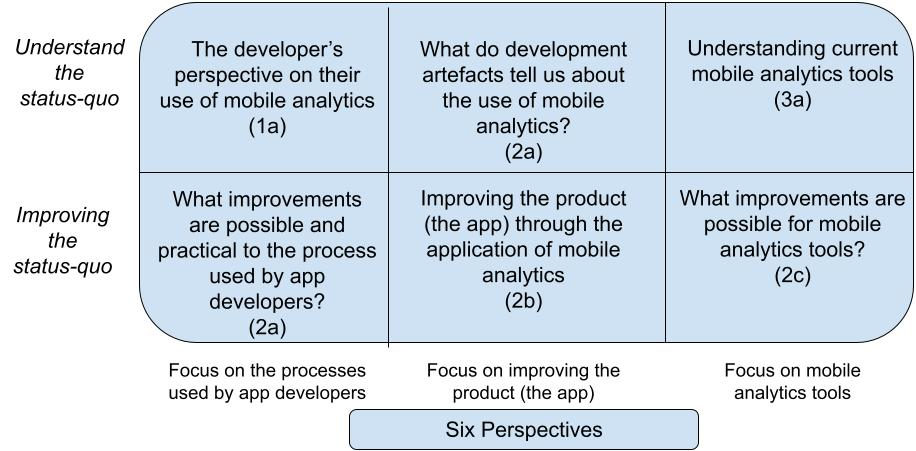
\includegraphics[width=15cm]{images/my/six-perspectives-2x3-matrix-25-oct-2021abc.jpeg}
    \caption{Six Perspectives (repeated for the case studies)}
    \label{fig:six-perspectives-in-case-studies}
\end{figure}


The case studies apply the six perspectives (illustrated in Figure~\ref{fig:six-perspectives-in-case-studies}) that were introduced to help answer the main research question by using three distinct approaches of applying Mobile Analytics to Android apps
~\footnote{Android apps were selected to enable the use of Google Play Console reports and analytics, including Android Vitals; nonetheless one of organisations studied chose to also include analytics in their iOS app, so this will also be covered briefly.}. Each study contributes to at least one of these six perspectives. In practice they all contribute to several and may contribute to most of them. 

\textbf{Challenge: how to structure the studies in the thesis} As each study contributes to a range of the perspectives, I find it hard to decide on a way to report on the various studies clearly so the reader can maintain focus and clarity in terms of the readability of the research\footnote{
\textbf{Marian's suggested gameplan} 
I need to provide for each study:
Context and orientation; then drive from the [6] perspectives.
A suggested order: Status Quo slice, then what happens if we interfere?
}.

\begin{enumerate}
    \item The first approach is to learn what app developers do in terms of using mobile analytics for their apps. The material collected includes a mix of direct interactions, conversations, together with investigating various artefacts. These artefacts stem from two sources: 1) mobile analytics reports, and 2) the development team (\emph{e.g.} source control, bug reporting tools). Some developers provided direct access, others provided offline snapshots.
    \item The second approach is direct engagement with the project teams to facilitate more in-depth research. Two of the projects are opensourced, the rest are proprietary, commercial mission-critical apps. Each of these projects had their own needs in terms of their use of mobile analytics.  % Can we interfere / affect their behaviours
    \item The third approach focuses on the source code of various Android apps to investigate how the app developers incorporate analytics into their respective apps in terms of the types of information they recorded using the dominant in-app mobile analytics library: Firebase. The code provides a dispassionate perspective. % What do they do in terms of their code. 
\end{enumerate}

Several small experiments complemented the case studies, for instance to evaluate what is reported using both platform and in-app analytics. 
The research led to collaborations with two providers of mobile analytics, Google and Iteratively (since acquired and integrated into Amplitude); and provided insight into a wider range of mobile analytics tools.


\subsection{The rest of this chapter}

This chapter first introduces the methodology and repeatability aspects of case-studies for research into mobile analytics in \secref{section-methodology-ethics-and-repeatability-of-case-studies}. This is followed with another introduction into range of known data sources used in at least one of the case studies, in \secref{section-case-studies-data-sources}. 

Section \secref{section-field-reports-case-studies} presents the app developers' perspectives. 

The direct engagement case studies start with the two opensource case studies \secref{section-kiwix-case-study} and \secref{section-catrobat-case-study}. These are followed with extracts from one or more commercial projects in \secref{section-corporate-engineering-case-studies}, to protect the confidentiality of the organisation various details have been removed. Some representative and similar, `white-labeled' examples are also used to anonymise otherwise potentially sensitive characteristics of the source of the case study; where practical these have been made available as opensource projects to facilitate exploration and reproduction.

The source code perspective is in \secref{section-research-in-logging-practices}.

Where practical the experiments incorporate small opensource projects created for the respective experiments and are described in \secref{section-mini-experiments} and \secref{section-some-examples}. 

The collaborations with providers are covered in \secref{section-google-play-console-case-study} and \secref{section-iteratively-case-study}~\footnote{TODO consider whether to include the work with Appachhi.}. A summary of the various mobile analytics tools is covered in \secref{appendix-analytics-tools}

The final part of this chapter provides a summary of the various case studies \secref{section-summary-of-case-studies}. 

%%%% Marker for Julian - continue below here %%%%
\hrulefill
\clearpage
\section{Previous material follows}
\textit{The following content needs to be reevaluated and the stuff that's still relevant will be integrated earlier in this chapter.}
\begin{figure}[htbp!]
    \centering
    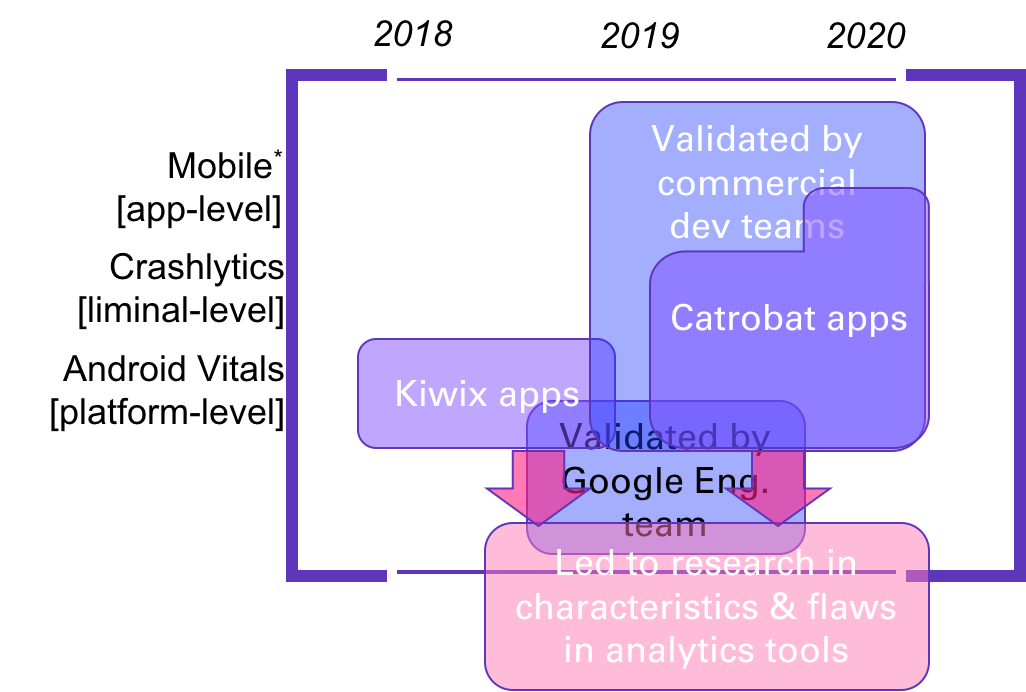
\includegraphics[width=10cm]{images/visual-connections-in-research.png}
    \caption{Visual Connections in my research}
    \label{fig:visual-connections-in-research}
\end{figure}

\textit{MUST-DO update this figure, it is out of date.} Figure \ref{fig:visual-connections-in-research}  aims to provide a visual overlay of the main practical elements of the research from 2018 to 2020. There are three main factors: 1) the type(s) of analytics used, 2) the development team and their apps, and 3) the progression of the case studies, as they augment what has been learned in earlier case studies.
% \akb{Why is it important to understand the timeline here - what implication does it have for understanding the research problem?}

The research started with the Kiwix~\footnote{The Kiwix project enables people to use Wikipedia and other content offline~\url{https://www.kiwix.org/en/}} set of Android apps where the app with the highest crash rate, as reported by Google's Android Vitals, was used as the experiment to see if the crash rate could be improved. By design the Kiwix apps do not include any analytics or crash reporting to minimise the digital usage footprint of these apps as they may be used in areas of the world where Wikipedia is banned, \emph{etc.} where the users may be persecuted or even imprisoned. Nonetheless, as the apps were available through Google Play (amongst many sources), the development team received ongoing reports in Google Play Console including the Android Vitals reports on various `stability' metrics as defined and applied by Google.

The Catrobat team was and is an extremely well researched and supported collection of mobile apps intended to help young people learn how to enjoy developing games visually. It was established % Removed details for the review period: "by Professor Wolfgang Slany of" 
at the TU Graz university where both undergraduate and postgraduate students actively practice software skills on the codebase. My engagement started around June 2019, and we decided jointly to pick the thornier and most complex Android app - Pocket Code - as the subject for our collaboration and research, as it had proved to have an intractable ongoing issue with the high reported crash rate and was therefore a worthy challenge for the concepts proposed in my research. We had a reference app, called Pocket Paint, which had a lower crash rate. Note: Pocket Paint was and is incorporated into Pocket Code in addition to being a standalone app.

Pocket Code already incorporated one of the most popular crash analytics library called Crashlytics. At the time, it used an older, mature version of Crashlytics branded Fabric (a business first acquired by Twitter, then by Google). I have chosen to use the term \emph{liminal}~\footnote{\url{https://www.lexico.com/en/definition/liminal}} to indicate crash reporting is something that lives in the boundary layer between the app and the operating system, or platform. Either is able to observe application crashes, and for apps where both the app and the platform capture information about crashes the two data sources can be usefully cross-referenced and compared, as my research has done.

As Pocket Code was an Android app, available in Google Play, the team also received the reports provided by Google through Google Play. These two data sources provided an interesting and rich set of research challenges. 

Relatively recently, in February 2020, the Catrobat team had to migrate their Crashlytics reporting from the Fabric service, which Google was ceasing, to Firebase, the replacement reporting service Google provided. In parallel with this migration of the reporting, the project team agreed to incorporate mobile analytics into their Android and iOS apps. They decided to use Firebase Analytics for various reasons (to be covered later in my thesis), hence the extension of the apps into app-level analytics.

The two arrows in the figure indicate an area of unplanned research: 
%
I discovered various flaws in the developer-oriented reports Google provides to app developers who make their apps available in Google Play (approximately 2.9 million apps globally). This led initially to discussions with the relevant engineering teams for Google Play and Android Vitals at Google where they confirmed various flaws. They asked for ongoing updates on my findings and requested a report which I provided. Through our interactions and discussions, I realised the merit of researching the characteristics and flaws in analytics tools, and particularly those provided by Google for Android developers. This research is ongoing and intended to continue post-PhD given the importance and relevance of the topic.

In mid-2019 several commercial Android development teams learned of my research and offered to contribute their experiences and practices of using mobile analytics in their commercial apps. These apps include app-level analytics in addition to the development teams receiving the ongoing reports Google provides automatically. The contributions of these development teams helped provide additional weight to the value and relevance of using mobile analytics to identify flaws in mobile apps and evidence of the importance developers placed on addressing quality issues gleaned through these tools.

%\yy{The practical research}{Need to complete the sentences, what is liminal? Change Kiwix/Catrobat apps to "Kiwix/Catrobat teams"? }

\begin{table}[htbp!]
    \centering
    \small
    \setlength{\tabcolsep}{4pt} %% default is 6pt
    \begin{tabular}{llrr}
      Case Study &Role of Researcher &Apps &Active Users\\
      \hline
       \href{https://play.google.com/store/apps/dev?id=9116215767541857492&hl=en_GB}{Kiwix}  &Embedded &18 &367K\\
       \href{https://play.google.com/store/apps/developer?id=Catrobat&hl=en_GB}{Catrobat} &Guide &6 &200K\\
       \href{https://play.google.com/store/apps/dev?id=7665838187257770408}{Greentech Apps} &Observed &10 &987K\\
       \href{https://play.google.com/store/apps/developer?id=Moonpig.com&hl=en_GB}{Moonpig.com} &Observed &1 &130K\\
       \href{https://play.google.com/store/apps/details?id=boundless.moodgym&hl=en_GB}{Moodspace app} &Interviewed &1 &20K\\
       \href{https://play.google.com/store/apps/details?id=com.localhalo.app&hl=en_GB}{Local Halo app} &Observed &1 &1.1K\\
       Commercial case study &Consultant &1 &1.9M\\
       Analytics tools &Various &10\textsuperscript{6} &10\textsuperscript{9} \\
    \end{tabular}
    \caption{Project teams and Commercial apps in the case studies}
    \label{tab:case_studies}
\end{table}

For the Kiwix case study, the researcher has been an intrinsic long-term member of the diffuse project team, able to work directly with the code-base and collaborate directly with the developers and ancillary members of the project team. The second phase of the case study included collaboration during a week-long hackathon, the first of two case studies that used a hackathon as part of the research. 

For the Catrobat case study, the researcher advised and assisted the project team to apply mobile analytics to their larger, older, and less reliable app: \emph{Pocket Code}. The researcher helped lead a one-day hackathon and otherwise interacted through a bug reporting tool, JIRA, discussions and using shared documents. Pocket Code also included a crash-reporting library which allowed cross-tool comparisons of reports, analytics and data. During the research, the reporting platform for the crash-reporting was migrated to a newer service which provided further insights and comparisons across and between the various mobile analytics tools.

The Greentech apps case study blends public and private sharing of their projects, they track issues in public, the codebase is private. Their active userbase is larger than the combined userbases of the Kiwix and Catrobat mobile apps. The team structure is similar to those for the Kiwix project: it is a not-for-profit foundation where donations help fund some of the development work; however many of the development team members are part-time volunteers. Their core team are in Bangladesh, distant from the Western world, and their focus is to enable native Bangla speakers to learn and study the Quran. Their priorities differ from those of most projects; the quality of their material is paramount; and they sometimes disable support for apps that have serious quality flaws in these materials. 

For the commercial app teams (Moonpig, Moodspace, and LocalHalo), the researcher corresponded with one of the development team for each of the commercial apps and received either direct access to their analytics tools (LocalHalo), or was provided with snapshots (Moonpig and Moodspace). Permission was granted by their respective organisations for their contributions to be used for research purposes.

The corporate case study has an order of magnitude more complexity than the other apps with much higher demands on the software being reliable and performant. The business and the service provided through the client apps are expected to grow massively as the product matures and the software quality improves. While they include clients for MacOS, iOS, Android, webRTC, and Windows desktop operating systems, the case study focuses on the Android client.

How developers of Android apps actually use mobile analytics for remote logging compared to how developers use local logging focuses on the perceived purpose of the logging across over 100 opensource projects on GitHub.com. And the final case study is from the perspective of a startup who are developing and researching tools and techniques to help developers improve their design, implementation and use of usage analytics tools (both web and mobile apps). 

\subsection{TODO: Structure used to describe the case studies}
TODO describe Arosha's proposed structure and introduce its applicability and purpose here.

\clearpage
\section{Methodology, ethics, and repeatability of case studies} \label{section-methodology-ethics-and-repeatability-of-case-studies}

\begin{figure}
    \centering
    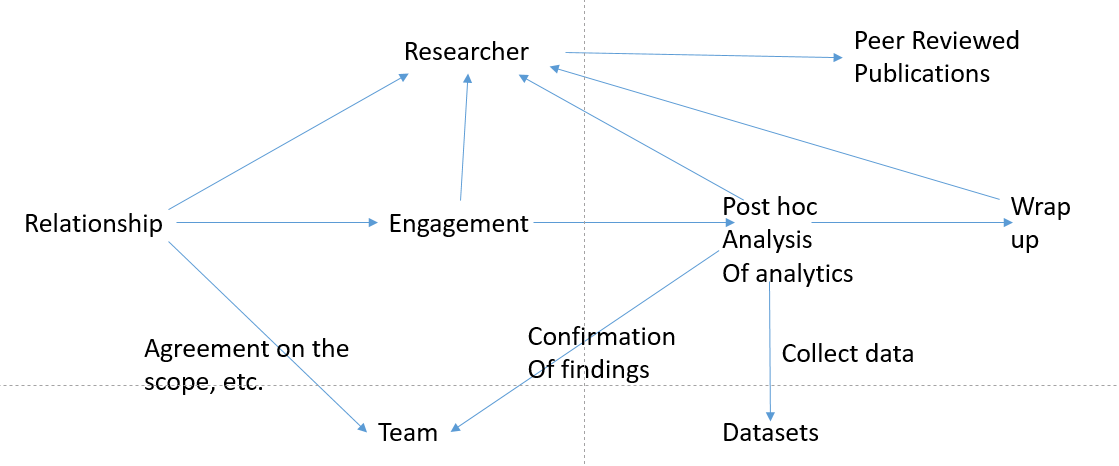
\includegraphics[width=14cm]{images/rough-sketches/Yijun-rough-sketch-of-relationships-in-case-study-methodology.png}
    \caption{Yijun's rough sketch of the methodology- a w-i-p}
    \label{fig:yijun-methodology-sketch}
\end{figure}




\subsection{Repeatability}
\textbf{Expand on:} What's hard to repeat (and why), aims to improve and demonstrate repeatability of the practices applied in this research.
\textbf{Absolutely key is what another researcher would do.}

One objective is to make the \emph{post-hoc} analysis repeatable, where others can perform the analysis and obtain similar results; therefore this section explains various patterns of analysis and there are various worked examples provided in the individual case studies.

\isabel{suggests repeatability is part of good research ethics.}
\isabel{Research as a political statement c.f. her transfer report.}

\begin{comment}
TODO papers to consider discussing here include: 
\begin{itemize}
    \item ``R3: repeatability, reproducibility and rigor"~\citep{vivek2012_r3_repeatability_reproducibility_and_rigor}

\end{itemize}
\end{comment}


\subsection{Research ethics for the case studies}
\label{section-research-ethics-for-the-case-studies}
\julian{Clarify what types of case studies: app, tools, both?}

The majority of the case studies presented in this research include other people. It is right and proper to ensure they and their respective organisations are willing to support the research directly - by participating - and/or indirectly - for instance by providing access to systems, tools, bug tracking systems, and so on. Some organisations require non disclosure agreements, and - in practice - they all choose what access to provide to what, to whom, and for how long. 

Engagement and trust need to be established with the people who manage the project and with the people who participate in the case study. Organisations often require approval from one or more senior representatives in the organisation, these may include head of development, and one or more of their legal, marketing, commercial, and risk departments.

For startups, one person may hold multiple roles, for instance in small startup teams they may be the CTO while also being an active developer of the software, \emph{and} the person responsible for operations, support and customer service. This was the case for two of the case studies presented in this research (LocalHalo and Iteratively), and in Moodspace the CTO was also the main developer of the app. In terms of obtaining permission, startups tend to be easy to work with if they agree to support the research as one or two people can quickly decide to support the research and provide access to whatever materials they are willing to share. They may not have time or patience to read or sign formal agreements, however an email summary of any verbal agreement helps to sum up that agreement and provide them the opportunity to confirm, clarify, or reject the contents of the agreement.


\newthought{General ethical considerations in ESSE}

An article jointly written by Singer and Vinson and published in 2002 was one of the first aimed at establishing guidelines and procedures for empirical studies in software engineering. \textbf{TODO complete the following: I addressed these in turn (as follows sub-sections) Relocate my current material into these 4 topics, else put it aside for now.} 

They proposed~\emph{``four core ethical concepts...: informed consent, scientific value, beneficence and confidentiality"}~\citep[p.1178]{singer2002_ethical_issues_in_empirical_studies_of_software_engineering} and they provided various examples of ethical issues in empirical studies of software engineering (\href{glossary-esse}{ESSE}). These four core ethical concepts are still relevant nearly 20 years on.

\newthought{How ethical issues applied to my case studies and why}

The case studies included people working with software together with the software artefacts they created, therefore there were, and are, ethical considerations that apply to these case studies. The considerations include all four of the core ethical concepts mentioned in the previous paragraph.

\begin{itemize}
    \itemsep0em
    \item \textbf{Informed consent}: participants and their respective organisations need to give informed consent in the work contained in the respective case study.
    \item \textbf{Scientific value}: the research has to be valid and relevant in order to justify the case study happening.
    \item \textbf{Beneficence}: aim to maximise the overall benefits for all the stakeholders and harm none. This includes the people who participate in the development teams, their organisations (where applicable), and the end users of their mobile app(s). 
    \begin{itemize}
        \item For the developers, they had the opportunity to use mobile analytics as they wished (including not using it) which offered them an additional technique and for some new skills.
        \item For the organisations, they had ongoing issues with the stability of their mobile apps and they would be able to benefit by having various stability issues considered and potentially addressed which would improve the stability and therefore the quality of their mobile app(s).
        \item For the end users, they did not contribute any additional information nor did they need to do anything beyond what they chose to do in terms of using and upgrading the respective app on their devices. Improvements in the quality of the app had the potential to improve their user experience when using the app, through the app being more reliable and performant.
    \end{itemize}
    \item \textbf{Confidentiality}: protect the confidentiality of participants and also protect the confidentiality of information provided and/or gleaned during the case study unless a) the work is in the public domain, b) permission has been granted to make the information public \textit{e.g.} as part of this research.
\end{itemize}

The case studies also involved development teams and their relationship with their organisation. 
As \citet[p.2]{robinson2019_applying_endosymbiosis_theory_tourism_and_its_young_workers} observe: \emph{``Business, or work, ecosystems are a community of interacting organisations and individuals (or groups) – or the organisms of the commercial world"}. Their research was into the relationships of tourism and its young workers, and the possibility for exploitation in either or both directions. The challenges in their domain may apply to this type of case study based research therefore the research was performed with due consideration of the potential adverse effects for any of the parties involved in the case study.

\newthought{Steps taken to mitigate the relevant ethical issues in the case studies}

For the hackathons the participants were volunteers who were already working on the respective opensource project. They freely volunteered to participate and their contributions in terms of development artefacts were (and are) public. Ethical approval obtained from the Open University for the workshop at the TestFest 2020 Conference in Poland. The ethics approval was requested as the workshop was intended to include personal, voluntary contributions of how the participants thought and felt about the use and efficacy of mobile analytics for software testing of the respective mobile apps. The workshop participants gave express consent for their contributions and any additional artefacts to be made public as part of the research. They were volunteers \textit{who wanted to actively participate in the workshop for their own intrinsic reasons - to learn and practice new skills, concepts, and mobile analytics tools.}

The participants were briefed and gave their permission either individually or on behalf of their organisations to use the material they freely provided. Several have reviewed my research and provided constructive feedback which has been applied. 
Note: It has not always been practical to reach all the participants, for instance some are no longer reachable.
%
Participants are anonymous with a couple of exceptions: 1) when the information is already public, 2) where they were happy to be identified in public as contributors to this research.  

The research did not involve other human subjects (such as the end users), the data is related to apps and how the app was used and how the app performed, humans were not and are not the subject of the research. No PII information was collected by the analytics tools used.

The majority of specific findings in this thesis are for opensource, freely available, apps without any restrictions on sharing the findings of the performance of the apps. 

The commercial project is subject to various professional legal agreements that include confidentiality and intellectual property considerations. Recreated, anonymous examples are used to protect the confidentiality of the the organisation, the development team, the app, and the artefacts.

For the interviews prior consent was requested and freely given. For the smaller organisations the participants were decision makers for the project and able to act on behalf of the project \textit{i.e.}, they did not need any additional approval. For the larger organisations, representatives of the organisation sought and obtained legal approval for the work covered in the respective case study.

Some of the opensource projects that form part of this research received and accepted pull requests from the researcher, these were freely given and freely received and have no known monetary value.

Note: during the case studies I was also a member of three relevant professional bodies: the British Computer Society (BCS), the IEEE, and the ACM, and worked to abide by their respective codes of conduct~\citep{bcs_code_of_conduct_2021, ieee_and_acm_code_1999on}.

\newthought{Beneficence: the need for beneficial relationships}

This research aimed and aims to provide benefit all the participants and for any relationships to be mutually beneficial.

Mutualism, commensalism, parasitism, predation and competition are five types of symbiotic relationship. % ``There are five main symbiotic relationships: mutualism, commensalism, predation, parasitism, and competition."  Symbiosis: The Art of Living Together https://www.nationalgeographic.org/article/symbiosis-art-living-together/ 
Of these the last three may produce adverse outcomes for at least one participant.

In computer science research that involves organisations and live projects the type or types of symbiotic relationship(s) are another key consideration. The candidate projects and their organisations need to be confident that if they participate as case studies in research that they will not suffer in the relationship. If they see mutual benefits of the research they may be more willing to actively participate. 




\newthought{Agency of participants and their organisations}

Another consideration is the concept of `agency' that the organisations and the relevant people are free to choose whether they wished to participate in the research. Some candidates declined to participate in the research on behalf of their project or organisation for various reasons. A common reason was lack of time on their part, another was that some candidates perceived the research would not be acceptable to their organisation, for instance owing to confidentiality or business risk.

The participants choose their model of engagement, this means the research needs to be adapted to their engagement model, availability, and ways of working. The researcher may need to bridge between and/or mediate between the academic research ways of working and those practiced in industry, and here in the domain of mobile app development. In particular the researcher needs to uphold the expectations of both academia and industry, this may be easier for someone who has sufficient experience and competence in both ecosysystems.

\newthought{How were these research concepts applied in this research?}

Every one of the actual case studies, and those that did not come to pass, started with a connection between two or more people. Sometimes the connection was indirect via someone who knew of the research. In several cases the relationship was established by someone at the candidate case study who was aware of the researcher and the research. There will be other ways to recruit potential case studies, however they were not used for this research.

However an initial contact/communication came about thumbnail of the research was presented to the candidate. This included an explanation that at least some of the work would need to be permitted to be published as part of the research and that permission would need to be freely given. With the exception of a particular commercial case study the engagement was voluntary and unpaid. The particular commercial case study ran alongside a paid consultancy where the researcher was engaged to help address challenges in one or more projects with similar aims to this research. Details of the organisation, the project(s), and the particular results are constrained by a commercial non-disclosure agreement.

For the two direct engagement case studies for opensource projects, they both asked for help to improve the reliability of at least one of their Android apps. Therefore the engagement had the potential to be mutually beneficial. Similarly, for the case studies with mobile analytics tool/service providers they saw value in being engaged with the research and the immediate results of those case studies. For the developer interviews the symbiotic relationship was closest to being commensal, while they may glean some benefits, it was not a primary factor in their willingness to participate. Instead they were keen and willing to help with the research for the good of the research. 


\begin{comment}
\begin{itemize}
    \item Ethics review for Workshop in Poland (and then for various reasons the contents of the workshop were not viable because of the effects of COVID-19.
    \item No other human subjects, the data related to apps and how the app is used and performs, humans are not the subject of the research.
    \item Opensource, freely available apps without any restrictions on sharing the findings of the performance of the apps. No PII information collected by the analytics tools used.
    \item Semi-structured interviews with various individuals in their professional and/or project capacities.
\end{itemize}
\end{comment}



\begin{comment}
TODO papers to consider discussing in the ethics section include: 
\begin{itemize}
    \item ``The human is the loop: new directions for visual analytics"~\citep{endert2014_the_human_in_the_loop_new_directions_for_visual_analytics}
    \item ``Not All Trust Is Created Equal: Dispositional and History-Based Trust in Human-Automation Interactions"~\citep{merritt2008_not_all_trust_is_created_equal_etc}.
    \item \emph{``Symbiosis
Symbiosis refers to the partnership (usually long-term) that is established between two or more organisms. In microbiology, symbiotic relationships are often established between a microorganism and its host, and the partnership can be mutualistic or parasitic."} \url{https://www.nature.com/subjects/symbiosis}
\end{itemize}
\end{comment}

\clearpage
\chapter{Data sources}
\label{app:data-sources}

There are various sources of relevant data in terms of my research and research into mobile analytics necessarily includes the data and reports that are made available through mobile analytics. These data and reports are primarily aimed at the development teams responsible for the respective mobile apps. Other data sources include source code and bug tracking systems. 

Various development teams made at least some of their mobile analytics reports, data, source code, and/or bug tracking systems available for research purposes. Some provided occasional snapshots, others access for a period, and some provided access on a long term basis.

\section{Characterising the data as presented}
The providers of the analytics services choose and constrain what data is available, to whom, and for how long. App, developer, and organisation specific mobile analytics are private and only available to authorised users of the respective services and accounts.

The analytics services present their data in at least one form, the most common being via web pages that include visual reports. The others include: file downloads, API access, proprietary mobile apps, and vendor specific exports to one or more cloud-hosted services. Some also provide integration with issue/bug management tools.

Examples of web pages include the two shown in Figure~\ref{fig:examples-of-sentry-io-mobile-analytics-reports} from \href{https://sentry.io/}{sentry.io} which show the ranked set of recent issues detected by \href{https://sentry.io/}{sentry.io} for the LocalHalo app, and the two shown in Figure~\ref{fig:examples-of-gpc-with-av-mobile-analytics-reports} from Google Play Console for the main Kiwix Android app. 

\begin{figure}
    \centering
    \subfloat[Issues Report]{{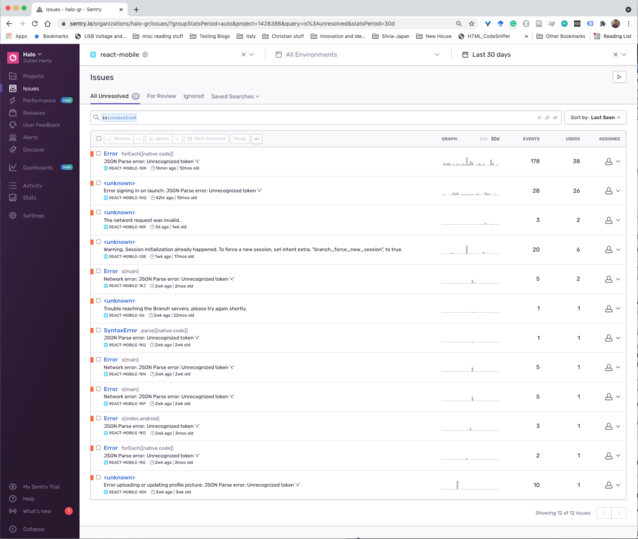
\includegraphics[width=6cm]{images/sentry.io/sentry.io-issues-page-resized.png} }}
    \qquad
    \subfloat[Individual Error Details]{{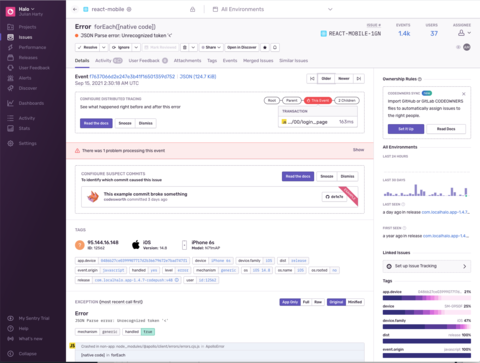
\includegraphics[width=6cm]{images/sentry.io/sentry.io-error-page-resized.png} }}
    \caption{Examples of sentry.io mobile analytics}
    \label{fig:examples-of-sentry-io-mobile-analytics-reports}
\end{figure}

\begin{figure}
    \centering
    \subfloat[Dashboard for Kiwix]{{\includegraphics[width=6cm]{images/android-vitals-screenshots/kwix/resized-example-for-kiwix-dashboard-2021-sep-16.png} }}
    \qquad
    \subfloat[ANR's for Kiwix in Android Vitals]{{\includegraphics[width=6cm]{images/android-vitals-screenshots/kwix/resized-example-of-android-viatals-anr-chart-2021-sep-16.png} }}
    \caption{Examples of Google Play Console mobile analytics}
    \label{fig:examples-of-gpc-with-av-mobile-analytics-reports}
\end{figure}
% Thanks to https://resizeimage.net/ for enabling easy resizing of the screenshots and 
%  https://www.codegrepper.com/code-examples/whatever/how+to+set+two+images+side+by+side+in+latex for the above latex.

When the data is presented visually (as web pages or in mobile apps) many of the reports are interactive, and some can be customised to varying degrees. The contents are often dynamic and recent, and therefore ephemeral. While reports these are useful for developers they do not necessarily facilitate further processing, storage, or analysis of the underlying data. Web scraping is one approach to extracting data from web pages; \href{section-vitals-scraper}{\nameref{section-vitals-scraper}} was developed as part of this research to preserve reports and data from Google Play Console with Android Vitals. The challenges, design, and implementation are discussed in that section of this thesis. In terms of this topic, data sources, Vitals Scraper enabled copies of visual reports in Google Play Console to be preserved as PDF files, summary data to be exported as a CSV file. It also exported and crash and ANR clusters were exported from Android Vitals in the JSON format.

Interactive downloads reduce the need to parse web pages that contain the same underlying data and therefore a mechanism to improve the working life of the data, however in practice often they contain a small subset of the data. They are also a static snapshot, \textit{i.e.} they are not updated by the provider once they have been downloaded. A germane example of one of the extracts available from a visual report in Android Vitals is illustrated in Listing~\ref{listing:crash-stack-trace-in-kiwix}. This facility was added to Android Vitals in 2021 and a good example of how providers change the capabilities and features of their mobile analytics from time to time.

Google Play Console also provides various downloadable daily summary reports. The details change from time to time, the current details should be available online at \url{https://support.google.com/googleplay/android-developer/answer/6135870}.

{\footnotesize
\begin{quote}
    `Control access to Google Cloud Storage
    Reports available on Google Cloud Storage use the same access restrictions that control data access on your Play Console. This means account users with access to areas of a Play Console account have access to the corresponding reports in Google Cloud Storage.
    
    Account owners can update permissions for individual users at any time.
    
        To access bulk reports, your "View app information" permission must be set to "Global."
        To download financial reports, your "View financial data" permission must be set to "Global." '
\end{quote}}~\citep{google_play_download_and_export_monthly_reports}~\footnote{in 2020, this help page  \url{https://support.google.com/googleplay/android-developer/answer/6135870} stated the developer's user account needed to be given 'Global' permission rather than per-app. In 2021 the same article no longer explains what permissions are needed, however another help page \url{https://support.google.com/googleplay/android-developer/answer/9844686} partly answers the permissions that needs to be granted.}

Here are the instructions for how to change the setting to Global \url{https://support.google.com/googleplay/android-developer/answer/2528691}

Where and when the data is available using APIs and/or available for ongoing cloud-based processing there is the greatest flexibility and opportunity for development teams (and others with access) to perform ad-hoc and ongoing analysis. When providers do offer these services, they sometimes need to be paid for on an ongoing basis. 

\begin{lstlisting}[language=json, caption=Exported contents for a crash reported in Android Vitals in Sept 2021, label=listing:crash-stack-trace-in-kiwix]
  java.lang.IllegalStateException: 
  at androidx.fragment.app.Fragment.requireContext (Fragment.java:805)
  at androidx.fragment.app.Fragment.getResources (Fragment.java:869)
  at androidx.fragment.app.Fragment.getString (Fragment.java:891)
  at org.kiwix.kiwixmobile.core.main.CoreReaderFragment.webViewFailedLoading (CoreReaderFragment.java:1478)
  at org.kiwix.kiwixmobile.core.main.CoreWebViewClient.onReceivedError (CoreWebViewClient.java:112)
  at android.webkit.WebViewClient.onReceivedError (WebViewClient.java:298)
  at fz.handleMessage (chromium-Monochrome.aab-stable-457706223:125)
  at android.os.Handler.dispatchMessage (Handler.java:109)
  at android.os.Looper.loop (Looper.java:166)
  at android.app.ActivityThread.main (ActivityThread.java:7555)
  at java.lang.reflect.Method.invoke (Native Method)
  at com.android.internal.os.RuntimeInit$MethodAndArgsCaller.run (RuntimeInit.java:469)
  at com.android.internal.os.ZygoteInit.main (ZygoteInit.java:963)
\end{lstlisting}

\section{Google Play}
Google Play provides a public end-user orientated visual view of apps in Google Play. It also provides a developer-oriented view of \emph{their} apps\footnote{More correctly, apps they are permitted to view and manage. Google provides account owners the ability to invite people to view, and potentially manage, one or more Android apps. Not everyone who has access is a developer, nonetheless the reports, tools, etc. are aimed primarily for developers.}; this is known as Google Play Console.

\section{Google Play Console}
Monthly reports are available for developers to download, they include: Install statistics, Crash statistics, Rating statistics, Reviews and Retained installers. 

Google provides several online help pages on the monthly reports~\citep{google_play_download_and_export_monthly_reports}. They do not describe the fields or the character encoding of the contents of the files. The files start with a two-character code \texttt{0xFE 0xFF} which indicate the contents of the file is encoded as UTF-16 little-endian. These seemingly useful characters can prevent the content from being loaded in many programs and utilities intended to work with CSV data.

\subsection{Defunct reports}
Various reports used to be available to download, Google chose to remove them~\citep{google_play_download_and_export_monthly_reports}. The removed reports include: subscription acquisition (removed November 2019), detailed crash and detailed ANR reports (removed May 2018).

\subsection{Coping with UTF-16 content}
Google provides the files encoded in UTF-16 format. The default import tool in the R programming language fails to import data in this (or many other encodings). Through research and experiments the following code snippet is able to load downloaded crash reports into a Data Frame in R.

\begin{lstlisting}[language=R, caption=Processing UTF-16 contents using R, label=listing=processing-utf-16-contents-in-r]
  setwd("\textbf{$_{\widetilde{~}}$}")  %All this to display a tilde adequately.
  filenames = list.files("./Dropbox/Google Play Console Reports/reports/kiwix/", pattern = ".csv")
  directory = "./Dropbox/Google Play Console Reports/reports/kiwix/"
  filenames <- paste(directory, filenames, sep="/")
  CrashAndAnrStats <- lapply(filenames, read.csv, fileEncoding="UTF-16")
\end{lstlisting}

Data I downloaded (not necessarily used) include reviews stored in Google Drive.

\subsection{Obtaining the data}
Google provide two documented ways to obtain the reports. The simplest for occasional use is to download the reports from the relevant \emph{Download Reports} section in Google Play Console. The second is to configure and use the \texttt{gsutil} command-line tool.

\subsubsection{Interactive per-file downloads}
The interactive GUI for download reports leads to three menu options: Reviews, Statistics, and User acquisition. Statistics includes three types of information: Install statistics, Rating statistics, and Crash statistics. The other two menu options offer a single type of information: \emph{Reviews}, and \emph{Retained installers} for user acquisition.

\subsubsection{gsutil}
Google provides a command-line tool called \emph{gsutil}\footnote{Perhaps the name is based on \underline{G}oogle \underline{S}torage \underline{util}?} which can be used to download reports in bulk. While Google encourages people to create and configure a Google Cloud account and use gsutil from the Google Cloud sdk, they also provide the file as a separate download together with installation~\footnote{Installation instructions for gsutil \url{https://cloud.google.com/storage/docs/gsutil_install}} and configuration instructions~\footnote{\url{https://cloud.google.com/storage/docs/gsutil_install\#creds-gsutil}}. I chose to use the standalone version of gsutil and was able to install and configure it without problems.  

Example command-lines are provided in the documentation, these need to be edited to point to the correct project bucket for a given app's data, and similarly unless all the files are to be downloaded, a suitable wildcard provided for gsutil.  
% https://cloud.google.com/storage/docs/quickstart-gsutil

%%%% Example command-lines
% gsutil -m cp -r gs://pubsite_prod_rev_14876298819229479527/stats/crashes/crashes_org.kiwix.kiwixcustomphet_20* .
% gsutil -m cp -r gs://pubsite_prod_rev_14876298819229479527/stats/installs/installs_org.kiwix.kiwixcustomphet_20* .

\subsection{Installs}
Installs are important as one measure of success of an app. Mainstream Android apps need to be installed before they can be used (unlike web apps, for instance which are not explicitly 'installed'). 

\subsubsection{Assumptions for Installations } 
One assumption is that new apps should start with no installs, the second is that there are more installs than uninstalls, in other words the total number of uninstalls cannot exceed the total number of installs (assuming they are measured and counted similarly).

Analysing Installs: 
\begin{enumerate}
    \item Obtain data from Google Play
    \item Gather data from files into linear list, coping with changes in file structure over time.
    \item Interpret fields as best possible.
    \item Estimate which fields are correctly populated.
    \item Generate equivalent reports to those presented in Google Play Console.
\end{enumerate}

\subsubsection{Fields change over time in files}
We observed several changes in the contents of the monthly files with three different formats in the first six months of the installs files for the Chemistry and Physics Simulations Kiwix app. These changes made the data harder to compare and analyse as several fields are not consistently available over the history of the data.
% (a) Date,Package Name,Current Device Installs,Daily Device Installs,Daily Device Uninstalls,Daily Device Upgrades,Current User Installs,Total User Installs,Daily User Installs,Daily User Uninstalls
% (b) Date,Package Name,Current Device Installs,Daily Device Installs,Daily Device Uninstalls,Daily Device Upgrades,Current User Installs,Total User Installs,Daily User Installs,Daily User Uninstalls,Active Device Installs
% (c) Date,Package Name,Daily Device Installs,Daily Device Uninstalls,Daily Device Upgrades,Total User Installs,Daily User Installs,Daily User Uninstalls,Active Device Installs
\begin{table}[htbp!]
    \centering
    \footnotesize
    \begin{tabular}{lll}
    (a) &(b) &(c)\\
    \hline
    Date &Date &Date\\
    Package Name &Package Name &Package Name\\
    Current Device Installs &Current Device Installs &\\
    Daily Device Installs &Daily Device Installs &Daily Device Installs\\
    Daily Device Uninstalls &Daily Device Uninstalls &Daily Device Uninstalls\\
    Daily Device Upgrades &Daily Device Upgrades &Daily Device Upgrades\\
    Current User Installs &Current User Installs &\\
    Total User Installs &Total User Installs &Total User Installs\\
    Daily User Installs &Daily User Installs &Daily User Installs\\
    Daily User Uninstalls &Daily User Uninstalls &Daily User Uninstalls\\
                          &Active Device Installs &Active Device Installs\\
    \end{tabular}
    \caption{File Formats for Installs}
    \label{tab:file_formats_for_installs}
\end{table}

The changes in the columns means that more work is needed to combine the data consistently for reporting and analysis. 

\begin{lstlisting}[language=R, caption=Code snippet in R showing the error reported when columns in the data to import do not match, label=listing:r-import-error-code-snippet]
installs_data <- do.call(rbind, installs)
Error in rbind(deparse.level, ...) : 
  numbers of columns of arguments do not match
\end{lstlisting}

An article by Amy Whitehead~\footnote{\url{https://amywhiteheadresearch.wordpress.com/2013/05/13/combining-dataframes-when-the-columns-dont-match/}}, together with comments to that article \emph{e.g.} on using \texttt{Reduce()} enabled the data to be loaded despite differences in the columns.
% Also interesting ideas in https://stackoverflow.com/questions/26874710/how-does-one-combine-two-uneven-dataframes-to-create-a-full-species-matrix-for-a/26900774#26900774

\subsubsection{Processing Dates}
The source data files have the date as the first column in \texttt{YYYY-MM-DD} format. When these were loaded into R using \texttt{read.csv} the dates were converted into vectors. The dates are hard to process or analyse as vectors. 

The first approach was to use \texttt{flipDate} an opensource R package~\cite{r_date_conversion_github}, documentation is available in an online article~\cite{r_date_conversion_article}. \texttt{flipDate} is able to convert the dates stored as vectors into R's Date object. We used the \texttt{ymd()} method to do so.

The first approach was replaced by specifying a column class to the \texttt{read.csv} method~\cite{r_bloggers_using_colclasses}. Doing so improves both performance and utility of the data. It also removed the need to use \texttt{flipDate}.

\subsubsection{Dates in filenames}
The filenames represent monthly reports, as such, their name includes the 4 digit year and the month encoded in two digits, from 01 for January to 12 for December. The following listing provides examples of the first six filenames for installs for the Pocket Code.

\begin{comment}


\begin{lstlisting}[language=R, caption=Querying installs using R, label=listing=using-head-for-installs-in-r]
head(install_filenames)
[1] "installs_org.catrobat.catroid_201308_overview.csv"
[2] "installs_org.catrobat.catroid_201309_overview.csv"
[3] "installs_org.catrobat.catroid_201310_overview.csv"
[4] "installs_org.catrobat.catroid_201311_overview.csv"
[5] "installs_org.catrobat.catroid_201312_overview.csv"
[6] "installs_org.catrobat.catroid_201401_overview.csv"
\end{lstlisting}

\end{comment}

%%%% Useful articles include:
% https://stackoverflow.com/questions/17496358/r-help-converting-factor-to-date
% https://www.displayr.com/r-date-conversion/ (mentioned above)
% https://stackoverflow.com/questions/32854538/converting-a-character-string-into-a-date-in-r
% https://www.r-bloggers.com/using-colclasses-to-load-data-more-quickly-in-r/
% https://stackoverflow.com/questions/5158179/processing-date-and-time-data-in-r
% https://www.r-bloggers.com/date-formats-in-r/

The \texttt{Date} datatype enables dates to be analysed and compared \emph{e.g.} \texttt{min("my\_date")}~\cite{r_bloggers_date_formats_in_r}.


\subsection{Crash and ANR Reports}
Google Play Console only provides the Crashes and ANRs in a combined summary report. We created and opensourced \href{https://github.com/commercetest/vitals-scraper}{Vitals Scraper} to enable additional data to be downloaded, including details of crashes and ANR's.

For the summary reports provided by Google Play Console, in \texttt{R} the data was first loaded file by file, each into a distinct \texttt{data.frame}. These are then combined into a single larger data set as follows:  
\texttt{do.call(rbind, crash\_and\_anr\_stats)}\footnote{Using the initial naive approach is enough to obtain the behaviour I sought \url{https://www.r-bloggers.com/concatenating-a-list-of-data-frames/}}

\begin{lstlisting}[language=R, caption=Querying daily crash and ANR statistics files using R, label=listing=using-head-for-crashes-and-anrs-in-r]
head(crash_and_anr_stats[[1]])
        Date         Package.Name Daily.Crashes Daily.ANRs
1 2014-01-02 org.catrobat.catroid             1          0
2 2014-01-04 org.catrobat.catroid             1          0
3 2014-01-05 org.catrobat.catroid             1          0
4 2014-01-11 org.catrobat.catroid             1          0
5 2014-01-12 org.catrobat.catroid             1          0
6 2014-01-14 org.catrobat.catroid             1          0
\end{lstlisting}

We can observe there are dates without data, for instance \nth{3} January 2014 for Pocket Code. One possibility is there were no reported crashes or ANRs for the dates that are not in the reports, Google does not document the contents of the files, so the reason is not known currently.

\section{Fabric Crashlytics}
Fabric Crashlytics and the associated Android programming library and APIs has been used by the Pocket Code Android app for several years, predating my involvement. It was retired by Google in early May 2020, they replaced it with the Firebase Console for the reporting. They also offer a replacement library and APIs which the project has  yet to switch to.

The reports in Fabric and the replacement Firebase console are predominantly graphical and visual in nature. Fabric allowed some of the data in the reports to be exported. Details and examples TBC %MUST_DO continue this section.

\section{Microsoft AppCenter}
We used Microsoft AppCenter with the Zipternet Android app we developed for various reasons, including this research. It is another tool predominantly graphical and interactive in nature.
% MUST_DO extend this section and provide some examples. I need to log back into AppCenter too, I need to remember how I originally logged in though :)

\section{Summary of Data Sources}
My research analysed data using various sources for several case studies. 

\section{Field Reports from Commercial App Developers}~\label{section-field-reports-case-studies}
The research includes field reports from developers of three distinct commercial Android apps. Each uses mobile analytics in their regular software development practices.

\subsection{Characteristics of the commercial apps}

\begin{itemize}
    \item Technologies
    \item Analytics available to the team
    \item Development priorities for their use of analytics
\end{itemize}

\subsection{Moonpig}

\begin{figure}
    \centering
    \includegraphics[width=13cm]{images/android-vitals-screenshots/moonpig/real-time-crashes-Screenshot-2019-06-10-at-15.42.34.png}
    \caption{Android Vitals: Moonpig snapshot of top crashes \nth{10} June 2019}
    \label{fig:av-moonpig-top-real-time-crashes-10-jun-2019}
\end{figure}

In Figure~\ref{fig:av-moonpig-top-real-time-crashes-10-jun-2019} Android Vitals shows the most frequent crash clusters for the production releases of the Moonpig Android app. The majority of crashes were an \texttt{IllegalStateException} in a third-party library SpiceManager, part of the RoboSpice opensource project https://github.com/stephanenicolas/robospice . 

This crash is an excellent example of how changes and new developments in the ecosystem can render what was reliable working software into software that is no longer fit for purpose, \emph{i.e.} RoboSpice was developed in 2012 to help developers simplify coding of asynchronous networking requests https://github.com/stephanenicolas/robospice and the library worked really well at the time and for several years afterwards. It became popular as a result and was used widely by many teams, including at Moonpig. However, as the Google Android platform morphed some of the changes to Android were incompatible with RoboSpice. And with Android Oreo (Release 8.0) changes to the way background services worked broke the functionality of the library sufficiently that the project was archived by the creator and project owner https://github.com/stephanenicolas/robospice/issues/467 

For apps that used RoboSpice the crash rate increased on the newer releases of Android, for example Figure~\ref{fig:av-moonpig-crash-rate-groupings} shows the crash rates by Android version were lowest on Android 7, higher for Android 8 and 8.1, and significantly higher again for Android 9. The teams needed to allocate time and energy to finding a suitable alternative to RoboSpice and then implement and test the new approach. Android Vitals helped provide an indication of the effects of the crashed and therefore provided evidence the development team could use to assess and prioritise the work.

\begin{figure}
    \centering
    \includegraphics[width=13cm]{images/android-vitals-screenshots/moonpig/Screenshot 2019-06-10 at 15.41.23.png}
    \caption{Android Vitals: Moonpig various groupings of the crash rate \nth{10} June 2019}
    \label{fig:av-moonpig-crash-rate-groupings}
\end{figure}

\subsection{Moodspace}
Moodspace is an Android app aimed at improving mental health through various exercises incorporated into the app. It was released in 2019, with over 150K downloads by early 2020~\citep{objectbox2020_moodspace_interview}. Ian Alexander, the interviewee, was the software developer, co-founder, and runner of the company~\citep{objectbox2020_moodspace_interview} so he combines technical and operational responsibilities. He is an experienced app developer and also trained as a chemical engineer.  % https://www.linkedin.com/in/ian-alexander-01353340/

(\nth{13} June 2019)
% Source https://mail.google.com/mail/u/0/?q=kiwix+crash+rate+#search/kiwix+crash+rate/KtbxLzGHgCVznXxsGDjVgJGLFwmmGXxvxq
I love Android vitals - especially \textbf{core vitals}. Seeing your app in comparison to apps of peers provides some great motivation to step up your game. The only issue I have with core vitals is that I can't see them all! We are by no means a big app, so don't have enough data to meet googles standard for anonymised results, so results for most of the core vitals are hidden. I don't quite understand why this should be the case as the headline figure of your apps performance surely doesn't have to rely on anonymous data? Whereas the drilled down details of a core vital should be anonymous, so maybe the details view could just be blocked instead of hiding the entire core vital? To give context, MoodSpace has at least 4k monthly users, so there must be plenty of apps which get little or no use form core vitals, simply from them being hidden.

As for the other tools Google provides:
\begin{itemize}
    \item \textbf{ANR \& crashes} - I usually use crashlytics, so never really use this tab. the reason being, that the play console used to be very unreliable for crashes. But by the looks of it, it seems to have improved a lot, and pretty much matches the crashes I see in crashlytics now. Looking at it now, I actually noticed an ANR which could probably be fixed!
    \item \textbf{Pre launch reports} - I don't usually use this. Although this tool provides a nice safety net, it's quite basic, so any bugs that would cause the pre launch tests to fail have been found pre uploading through some quick manual testing. I actually ended up ignoring most pre launch reports when accessibility problems used to trigger failures, as we don't really have the resources to handle accessibility for now. But this seems to have changed in the last few months and accessibility problems don't cause a host of errors - maybe a way to ignore issues would be useful? In fact, pre-launch reports currently don't run on my app and fail with an incompatible apk error, not too sure why thats the case...
    \item \textbf{App signing} - very useful! and always use this since it was added.
    \item \textbf{Seperate release tracks} - love them! Especially since the addition of the internal track. The only issue was that I couldn't easily distribute debug versions of the app from the play store, and had to use a 3rd party tool to achieve that. Although Google have recently added Internal app sharing which should remedy that problem - however, I haven't figured out how to integrate that into our continuous integration process quite yet.
    \item \textbf{App bundles} - I'm still trying to integrate this, but as our new apps going to be heavily illustrated, this should cut our apk size significantly
\end{itemize}

As for several things I think are missing:

\begin{itemize}
    \item A gradle plugin to integrate play store uploading into CI processes. I currently use a 3rd party plugin to do this, but it would feel a little more secure if it came from Google.
    \item Top line core vitals figures even if you don't have enough users!
    \item Someway for testers to download old apks from either internal app sharing, or the internal release track.
\end{itemize}

I've attached the ANR and crash rates for the app. As I say, I usually use Firebase crashlytics, so don't really fix crash issues from Play store data.

You're welcome to use any data or comments in your research! If you do use it, please send over a copy.

(\nth{15} June 2019)
I think there's two things which has helped keep the app quite stable:
\begin{itemize}
    \item The app has the benefit that it's been around for quite a while without any major features being added. So most updates have been small and incremental, which has gradually increased it's stability. (This may change when the new, big update drops...)
    \item The app doesn't use any api, so all datas stored in very fast ORM databases like object-box (and uses memory caching). This enables the app to be mostly synchronous, which hugely cuts down on complexity of code. i.e. no need to handle loading, errors, or concurrency. This is a bit benefit! And cuts down on errors significantly, with no real impact on performance for users. To illustrate that it has little impact on users, I use firebase performance to run a trace on some methods that call the ORM/cache - it's peak duration is 40ms while the majority of calls take 3-6 ms.
\end{itemize} 

Crashlytics only covers the crash report of Android vitals, so unfortunately there's no way to get things like battery usage of ANR reports unless Google makes those reports available :(. In terms of crashes, I'd always prefer Crashlytics to Android vitals, simply because there are added features like non-fatal reporting and logs which can make surfacing the cause of errors much easier (but do take need added effort to integrate compared to android vitals).

There's been a change of branding of the app development organisation to \href{https://play.google.com/store/apps/developer?id=Chachi+Productions&hl=en_GB&gl=US}{Chachi Productions}. \url{https://www.appbrain.com/dev/Chachi+Productions/}


\newthought{Notes to integrate into the case study}
\begin{itemize}
    \item \url{https://www.psycom.net/25-best-mental-health-apps} Helps set the context for these apps.
    \item \url{https://objectbox.io/moodspace-mobile-app-use-case/} An interview with the founder Ian Alexander on the technological choices, particularly objectbox as the database. He'd mentioned the performance was lightning fast and one reason the app was performant and reliable. 
    \item ``Built MoodSpace, a digital platform empowering everyone to take control of their mental health. MoodSpace began as a side project which later took on a round of funding and with a team of 6 supported a user base of 300k. Although no longer pursued as a business we continue to maintain the project and release regular updates to 10s of thousands of active users. The most recent iteration of the app was built with Kotlin, clean architecture, MVVM, Data binding, Gitlab CI, Coroutines/Flow, and ObjectBox and was architected to enable the use of Kotlin Multiplatform to share ~60\% of the codebase between platforms."~\url{https://www.linkedin.com/in/ian-alexander-01353340/}
    \item 4.18/5.00 User Experience rating \url{https://onemindpsyberguide.org/apps/moodspace/}
    \item ``To make the app work well at all we collect the following anonymous data:
    \begin{itemize}
        \item Crash reports: If you've never seen the app crashing, it's because as soon as one happens, we get a crash report. A little red light flashes in our office, a loud siren blares, and we release a fix right away. It's quite annoying actually.
        \item Analytics: We assume you're going to use the app a certain way. We're almost always wrong, and you often surprise us. Analytics lets us see how people like you actually use the app, so we can make improvements to the right places. Analytics can use the Google Advertising ID to identify you. This doesn't tell us anything about you (it's just some numbers and letters), but if you really want to trick us you can reset your Google Advertising ID at any time. Go to your device Settings > Google > Ads."
    \end{itemize}~\citep{moodspace2021_privacy_policy}
\end{itemize}


\subsection{Local Halo}
MUST-DO complete this sub-section on Local Halo.

\begin{table}[htbp!]
    \centering
    \small
    \begin{tabular}{ll}
       Question &Answer  \\
       Website &\url{https://www.localhalo.com/} \\
       Founded &2018\\
       Business Domain &Digital neighbourhood groups in UK.\\
       Business type &Startup \\
       Technologies  &React Native \\
       Analytics Available &Sentry, Mixpanel, Google Play Console \\
       Development Practices &Cross-platform development
    \end{tabular}
    \caption{Case Study Overview: Localhalo}
    \label{tab:local_halo_anaytics_overview}
\end{table}

\subsubsection{Experiences of using mobile analytics}
Localhalo incorporate two analytics libraries into their cross-platform mobile application: sentry for crash reporting and mixpanel for business-oriented usage analytics. For their Android app they also have access to Google Play Console.

They experience numerous crashes reported by Sentry, which occur within the React Native runtime environment. Sentry provides email alerts to the development team together with summary reports, (Figure~\ref{fig:localhalo-sentry-weekly-report-21-sep-2020} is example for the period~\nth{14} to~\nth{21} September 2020), and online access to their analytics.

A release in March 2020 had a high crash rate for the production release of their Android app. The top crash cluster was for:

\texttt{java.lang.RuntimeExceptionhost.exp.exponent.experience.a\$b.run}. 

This was traced to a problem in the expo library they used in the app~\url{https://github.com/expo/expo/issues/5839}. In that issue several developers for different Android apps provide data from Google Play Console confirming they also receive similar crash clusters. The cause has not yet been definitively traced or addressed, however for the LocalHalo app the crashes stopped being reported once a new release of the Android app, release 1.3.0, was released around \nth{6} April 2020.

\begin{figure}[htbp!]
    \centering
    \includegraphics[width=9cm]{images/localhalo/sentry-weekly-report-21-Sep-2020.png}
    \caption{LocalHalo: Sentry weekly report 14 - 21 September 2020}
    \label{fig:localhalo-sentry-weekly-report-21-sep-2020}
\end{figure}

\textbf{Sentry}

MUST-DO Check in Sentry for the various types of error. How actively are the development team reading, reviewing and addressing crashes being reported? 

\begin{figure}[htbp!]
\centering
\begin{minipage}{.5\textwidth}
  \centering
  \includegraphics[width=.8\linewidth]{images/localhalo/sentry-weekly-report-16-mar-2020.png}
  \captionof*{figure}{\nth{16} -~\nth{22} March 2020}
  \label{fig:localhalo-sentry-weekly-report-16-mar-2020}
\end{minipage}%
\begin{minipage}{.5\textwidth}
  \centering
  \includegraphics[width=.8\linewidth]{images/localhalo/sentry-weekly-report-23-mar-2020.png}
  \captionof*{figure}{\nth{23} -~\nth{29} March 2020}
  \label{fig:localhalo-sentry-weekly-report-23-mar-2020}
\end{minipage}
    \caption{Missing data reported in Sentry}
    \label{fig:sentry-missing-data-march-2020}
\end{figure}

\begin{comment}


\begin{figure}[htbp!]
    \centering
    %\subfigure[]{\includegraphics[width=0.4\textwidth]{images/localhalo/sentry-weekly-report-16-mar-2020.png}\caption{\nth{16} -~\nth{22} March 2020}\label{localhalo-sentry-weekly-report-16-mar-2020}}
    \subfigure[]{\includegraphics[width=0.4\textwidth]{images/localhalo/sentry-weekly-report-23-mar-2020.png}%\caption{\nth{23} -~\nth{29} March 2020}%\label{localhalo-sentry-weekly-report-23-mar-2020}
    }
    \caption{Missing data reported in Sentry}
    \label{fig:sentry-missing-data-march-2020}
\end{figure}
\end{comment}

%TODO fix the layout of the above figures: try: https://tex.stackexchange.com/questions/37581/latex-figures-side-by-side/37597#37597
Data missing from reports from~\nth{17} March to~\nth{25} March 2020 which affected the statistics around the time of the crashes related to Expo. Figure~\ref{fig:sentry-missing-data-march-2020} illustrates the gap across the two weekly reports. 

SHOULD-DO Consider summarising the crash totals per week. 

\textbf{MUST-DO} write up what we learn from the localhalo case study. external libraries can adversely affect the reliability of apps. Even small development teams can and do use multiple mobile analytics libraries. What can developers learn from the various reports provided by Sentry? How does cross-platform development in react-native affect the app reliability? are there crashes that only occur on Android or iOS? What's the correlation between crashes reported in Android Vitals and Sentry?


\subsection{Summary of Field Reports}
Active and ongoing use. 

%%% Ad-hoc notes from meeting Jakob D. Moonpig
% Business changes including the company's IPO mean the company has cut back on information they're willing to share internally and externally (e.g. for my PhD research).

\section{Greentech Apps}~\label{study-greentech-apps}

\subsection{Introduction to the Greentech Apps case study}
The aims and objectives of this case study include:

\begin{itemize}
    \item \textbf{A linear increase (+1)} : validation the methods described in my research are repeatable and scale to additional apps beyond the previous case studies.
    \item \textbf{Additional examples of characteristics of Google Play Console (+1)} :
    \item \textbf{A closed source case study (?)} : The previous case studies were all with opensource codebases so the code was available for bug investigation purposes. For this case study the source code and build processes are treated as a black box (it may potentially become a grey box case study if the development team share details of their engineering practices, etc.)
\end{itemize}

\subsection{Background to the Greentech Apps case study}
A set of Android apps developed and provided by Greentech Apps Foundation. They are described as modern Islamic Applications, according to their website \url{https://gtaf.org/}. The project encourages voluntary contributions, for instance to provide translations~\url{https://greentech.oneskyapp.com/collaboration/}. Their apps are popular, and well regarded. % MUST_DO add data on usage and ratings.


The project started in 2016 with the aim of enabling people to learn the Quran in the local language - Bangla - in Bangladesh. The project was started by a self-taught Android developer and his cousin Yemin, at the time an undergraduate student in computer science, who is now employed by the project in a hybrid role of software developer and project manager. The development team was predominantly volunteers until around 2018 when the first engineer was employed. In April 2020 the development team added two part-time paid developers and there are plans to grow the employed team including someone with UI and UX expertise. The team are funded through voluntary donations. From a research perspective my contacts at the project are Yemin and a fellow PhD student Riasat who also volunteers for the project.

At the start of the case study (June 2020) the team had ten Android apps published in Google Play~\url{https://play.google.com/store/apps/dev?id=7665838187257770408}. Of these apps, three are their core apps, and a couple are overdue an engineering revamp.  Two analytics tools are used for their core apps: Firebase Crashlytics and the default combination of Google Play Console with Android Vitals.

Their development team maintain their issues lists in public (\url{https://gitlab.com/greentech/}), the source code is private. They use a variety of languages and frameworks to develop their apps include React Native for at least one app (\href{https://play.google.com/store/apps/details?id=com.taskinator}{Taskinator}) and Java for the majority, they aim to use Flutter~\cite{flutter_dev_site} in future.

Exodus Privacy~\cite{exodus_privacy_project}, a non profit organization, was used to determine which analytics libraries are embedded in which of their apps as the source code was not available for these apps.

\textbf{SHOULD-DO} reformat the following as a table, or similar. Add the rest of their apps for completeness.

\href{https://play.google.com/store/apps/details?id=com.greentech.quran}{Al Quran (Tafsir \& by Word)} includes \href{https://reports.exodus-privacy.eu.org/en/reports/com.greentech.quran/latest/}{Google Crashlytics, Google Firebase Analytics}.

\href{https://play.google.com/store/apps/details?id=com.greentech.hadith}{	
Hadith Collection (All in one)} includes~\href{https://reports.exodus-privacy.eu.org/en/reports/77502/}{Google Firebase Analytics}.

\href{https://play.google.com/store/apps/details?id=com.greentech.hisnulmuslim}{	
Dua \& Zikr (Hisnul Muslim)} includes~\href{https://reports.exodus-privacy.eu.org/en/reports/54714/}{Google Firebase Analytics}. This app is available in two primary languages, English and Bangla (the mother tongue of where the core development team live, in Bangladesh). The \href{https://play.google.com/store/apps/details?id=com.greentech.hisnulmuslimbn}{Bangla} version of the app is several times more popular than the English release. Unlike the English version, the Bangla version of the app includes~\href{https://reports.exodus-privacy.eu.org/en/reports/146430/}{Google Crashlytics, Google Firebase Analytics}.

\href{https://play.google.com/store/apps/details?id=com.taskinator}{Taskinator} uses~\href{https://reports.exodus-privacy.eu.org/en/reports/146496/}{Firebase Analytics, OneSignal}.

Additional analysis by the researcher in July 2020 is available online in a Google Document that has been shared with two core members of the project team amongst others~\url{https://docs.google.com/document/d/1Ghu0UBXNrwOB3HYbgsPQ-OJV-fPmsP68lSLVRfcc4aA/edit?usp=sharing}.

\subsection{Development microcosm}
Who, how, where source and bug tracking take place. 

When do teams decide to fix which bugs, and what influences their decision making process?

NPE's and IndexOOBExceptions vs. IllegalStateException and native crashes.

The team have used Firebase TestLab to test some of the apps occasionally and the Robo testing performed automatically by the test lab has triggered various crashes in the apps being tested. One such example was where an app was missing a `resource'. The team fixed the build by adding the missing resource but did not explicitly retest the app afterwards in Firebase. 

\subsection{Applying analytics to the development practices}

The development team check Android Vitals approximately once a week, and Firebase more frequently as the team decided the crash reports in Firebase are more actionable. Perhaps unsurprisingly they check more often after new releases of their apps looking for any new bugs arising in the new release as it rolls out across the user population.



Differences noticed in their reports, however the focus is on the crashes reported in Firebase as they contain more contextual detail. ANRs seldom checked, considered to be less impactful on users and lower frequencies.

\subsubsection{Worked examples}
\textbf{This section needs redoing as the discussion with Yemin indicates they use Firebase predominantly}.
These worked examples are taken from Android apps developed and maintained by the Greentech team. They are taken on the \nth{7} and \nth{8} September 2020. They exemplify various aspects of the~\href{section-select-aggregate-scope-analyse-triage-and-prioritise}{\MakeLowercase{\emph{\nameref{section-select-aggregate-scope-analyse-triage-and-prioritise}}}} section. % SHOULD-DO find out why the section name still has an initial capital letter.



\subsubsection{Preserving the failure clusters}
Details of the crashes are recorded in individual issues on the respective project's GitLab site. The issue is cross-referenced in a note in the crash cluster reported in Firebase.

\subsection{Priorities of the project team}
Throughout 2020 and until April 2021 the team are focusing on bug-fixes which include fixing the causes of crashes in the apps. Three of the apps (four as one app is released as two distinct binaries) are in ongoing active development (\href{https://play.google.com/store/apps/details?id=com.greentech.quran}{Al Quran},~\href{https://play.google.com/store/apps/details?id=com.greentech.hadith}{Hadith Collection}, and~\href{https://play.google.com/store/apps/details?id=com.greentech.hisnulmuslim}{Dua \& Zikr}, which is also released separately in Bangla~\href{https://play.google.com/store/apps/details?id=com.greentech.hisnulmuslimbn}{{Dua and Zikr (Hisnul Muslim)}}~\emph{in Bengali}); and they plan to revamp two more of the apps (\href{https://play.google.com/store/apps/details?id=com.greentech.islamicquiz}{(Islamic Quiz)} and~\href{https://play.google.com/store/apps/details?id=com.greentech.salatbn}{Meaningful prayers (salat)}~\textit{in Bengali}, which was called salat in our interview).

% SHOULD-DO add support somehow for Bengali Unicode so I can replace the Anglicised app names with the correct ones. The issues are a mismatch between the compiler I'm using (pdfLatex) vs. the recommended packages to use
% e.g. 
% https://tex.stackexchange.com/questions/285507/how-can-i-use-bengali-script-in-an-english-document
% https://tex.stackexchange.com/questions/99606/how-to-write-bengali-in-latex
% https://www.overleaf.com/learn/latex/Multilingual_typesetting_on_Overleaf_using_babel_and_fontspec
% https://www.overleaf.com/learn/latex/international_language_support#Babel
% %%%
% https://www.researchgate.net/post/How_to_write_Bengali_unicode_text_in_English_document_in_Latex
% https://www.overleaf.com/learn/latex/arabic


\subsection{Summary of the Greentech Apps case study}
TODO complete this section, reflecting the topics raised in the introduction to the case study.
Integrate their comments on reducing the crashes and using analytics \url{https://gtaf.org/blog/gtaf-accomplishment-2020}.
\clearpage


%\setcode{utf8}

\section{Kiwix Android Apps}
\label{section-kiwix-case-study}
Relying on analytics and reports provided by the Google Android's platform and presented in Google Play Console, we were able to reduce the crash rates of a family of Android apps. 
%
We chose the most sophisticated and complex of the Android apps, which also had the highest Crash rate at the time (see Table~\ref{tab:gpc_kiwix_apps_11_feb_2019}). The reduction went from over 5\% to under 0.25\% during the case study.

Figure~\ref{fig:android-vitals-kiwix-android-crash-rate-vs-peers} provides an illustrative example of the crash rate for Kiwix Android. The comparison with its peers, apps in the same category across Google Play, also shows Kiwix Android was in the bottom 7\% in terms of crash rate in that category. So the app was unreliable by either measure.

By applying what the team learned about crashes reported in Android Vitals the team was able to reduce the crash rate of this app several fold. When the improved codebase was used to refresh various custom apps their crash rates also decreased several fold.

\begin{figure}
    \centering
    \includegraphics[width=13cm]{images/android-vitals-screenshots/Example-crash-rate-vs-peers 10-jun-2019.png}
    \caption{Android Vitals Kiwix Android crash rate vs peers \nth{10} June 2019}
    \label{fig:android-vitals-kiwix-android-crash-rate-vs-peers}
\end{figure}

Note: I have been involved in various aspects of Kiwix since 2014 including helping with the Android app, with manual and automated testing, with the PHeT project mentioned here, and so on.

\setminted{fontsize=\small,baselinestretch=1}

\subsection*{Evidence}
  \begin{minted}[
    gobble=4,
    frame=single,
    fontsize=\tiny,
    breaklines=true
  ]{yaml}
    evidence available :
      vitals-scraper : ~/sandbox/vitals-scraper-logs/android-stability-analysis/data/from-android-vitals
      google-play-console-reports : ~/Dropbox/Google Play Console Reports/reports/catrobat/pocketcode/crashes
      various-materials : in Dropbox
      co-written-paper : MOBILESoft 2019~\citep{harty_google_play_console_insightful_development_using_android_vitals_and_pre_launch_reports}, WAMA 2019~\citep{harty_better_android_apps_using_android_vitals}, MOBILESoft 2020~\citep{harty_improving_app_quality_despite_flawed_mobile_analytics}, ICST 2020~\citep{harty2020_how_can_software_testing_be_improved_by_analytics_to_deliver_better_apps}.
    evidence-needed : 
      Supporting materials for Phase 2:
      Supporting materials for Phase 3: 
      Releases and their release dates.
      Latest status of the tickets related  to crashes and ANRs.
      Current stability metrics for the Kiwix apps.
  \end{minted}

\subsection{Introduction of Kiwix Android Case Study}
%Introduce Kiwix at the risk of repetition. 
% TODO replace URLs with citations.
Kiwix makes knowledge available to people with no or limited internet access (\emph{i.e.} four billion people) by providing highly compressed content and a reader for the bespoke compression format. Anyone is free to use the software and the content. The project includes an offline reader for online content like Wikipedia, Project Gutenberg, or TED Talks and the project also develops and maintains software to download, compress, package, and make content easy to download and share~\citep{kiwix_about_the_project, gomez2017_wikimedia_kiwix_article}.

The project provides offline access to Wikipedia materials and many other read-only materials including TED talks, StackExchange sites, interactive science simulations, and others~\citep{kiwix_about_the_project, gomez2017_wikimedia_kiwix_article}. 

The Android project comprises various apps all based on a common opensource codebase. The core case study captures activities from early 2019 to early 2020; however the project is a long-term, ongoing project and I am still involved with it. Several post case-study updates will be covered in later chapters. The crash rate had been excessive for over a year and far exceeded the bad behaviour threshold Google Play specified. 

The case study started with a period of observation and discussion of the crash rate in particular as it had increased repeatedly and to such an extent that the 2.3 release had been aborted by the project team, various details follow.

In mid-April 2018 the reported crash rate was 1.53\%~\footnote{Details available in \href{https://github.com/kiwix/kiwix-android/issues/712}{issue 712} for the Kiwix Android project, the main app releases were version 2.2 and 2.3 at the time.}. By mid-June 2018 the overall crash rate had increased to 1.71\%~\footnote{The crash rate for version 2.2 was 2.03\% in the 30 days to \nth{14} June 2018.}. The rollout for 2.3 was aborted in February 2019~\footnote{The milestone for this release and the issues that were addressed is available online~\url{https://github.com/kiwix/kiwix-android/milestone/1?closed=1}.} as there was a crash that affected 10\% to 20\% of the users (according to the lead developer at the time). The crash rate for the app averaged over 5\% in January and February 2019. 


%\akb{Provide dates over which the excessive crash rate was noted? Also, while the project is a long-term, ongoing project, your case study captures its activity during a specific window.}

The project team actively exclude any tracking or analytics within the app to minimise the risk of harm to users of the app. This is because in some parts of the world Wikipedia is banned \url{https://en.wikipedia.org/wiki/Censorship\_of\_Wikipedia} and usage may result in oppression, prison, and so on. By design the app makes Wikipedia content freely available and easy to distribute peer to peer (and it has been downloaded in response to bans of the main Wikipedia web site~\url{https://twitter.com/KiwixOffline/status/968493031224733697?s=20}). The apps are also available on Google Play and the apps are popular there. The project team agreed they were willing to use the analytics Google Play provides about their apps and these analytics provide the basis for this case study.

Google Play obtains, processes, and provides analytics of Android apps from opted-in devices that incorporate Google Play Services (installed over 10 billion times \url{https://play.google.com/store/apps/details?id=com.google.android.gms&hl=en\_GB&gl=US} and installed on several billion Android devices (\url{https://en.wikipedia.org/wiki/Android_(operating_system) 2B+ in 2017}). These analytics include stability metrics for Android apps on those devices where developers are provided the analytics for their apps free of charge.
Note: Google Apps are available to download from third-party websites, particularly \url{https://www.teamandroid.com/gapps/}. 


The development team was relatively large and fluid ranging from teenagers to several professional developers and their active contribution periods ranged from weeks to many years~\footnote{Kiwix Android had 96 Contributors to the GitHub project at the time of writing~\url{https://github.com/kiwix/kiwix-android/graphs/contributors}}. The developers reviewed the code using pull requests.  The codebase included some application level automated tests; and the project included a continuous build, and used a commercial device farm provided free of charge by bitbar.com~\footnote{The tests were run using BitBar's custom \href{https://support.smartbear.com/bitbar/docs/integrations/gradle.html}{Gradle plugin} BitBar also providesinteractive testing on a wide range of devices, which helps with \emph{ad-hoc} testing, \href{https://github.com/kiwix/kiwix-android/pull/2350}{Issue 2350} provides a good example where the developers needed to test on a range of Android releases and had the facility to use this service.} 

One of the apps was chosen as the experiment and another as the control to determine whether the crash rate could be reduced through applying information Google Play provides in Google Play Console.

This was the first of the case studies and opened the research into the effects of applying analytics gathered at the platform (Android) level. Key distinctions include: the ability to perform a controlled experiment, to then see results of what happened when the experiment’s code was rolled out to the rest of the sibling apps, and the long terms effects of pursuing crashes and fixing them over a series of releases.

Key similarities include the use of Google Play Console analytics (virtually all the projects use it to varying degrees), and the improvements (reductions) in failures through applying the techniques. 

%\akb{I like this summary of the key differences and similarities}

\subsection{Context}
\textit{(Product/Project overview, Developer characteristics, tools, methods, key challenges for product/project).}

\subsubsection{Product/Project overview}
The Kiwix project was created in 2006 to help ensure people can access the \emph{``sum of all human knowledge"}~\citep{coillet2016-wikimedia-kiwix-ten-years}. Annually over a million people download it and the content packages the project creates and provides free of charge~\citep{coillet2016-wikimedia-kiwix-ten-years}.

It is mature as a project and led by several highly experienced contributors, where two volunteers co-founded the project and others joined over the years. From the outset the project has been open, and the software is also open sourced~\citep{sutherland2014_wikimedia_on_kelson}. It has received various grants and awards to help sustain the project and some of the funds pay for a hybrid mix of developers, where some are paid for at least some of their contributions. The Android codebase is one of many maintained by the project~\citep{gaudin2017_wikimedia_kiwix_android}. 

Various codebases, including Android, use and depend on another codebase written in C++ to process the custom ZIM file format developed by and for this project~\citep{gaudin2017_wikimedia_kiwix_android}. The open ZIM project (\url{https://wiki.openzim.org/wiki/OpenZIM}) and codebases are closely related and integrated with the Kiwix project and codebases, nonetheless it is distinct and separate.

\subsubsection{Design of the Kiwix family of apps}
Here is a brief overview of the relevant history of the codebase when the case study started. .

\begin{comment}
Additional material on Kiwix custom apps - possibly put in an appendix?

The project created a distinct opensource project for the creation of Android custom apps~\url{https://github.com/kiwix/kiwix-android-custom} At the time of the case study the build tools were very immature for custom apps.

\url{https://github.com/kiwix/kiwix-android-custom/blob/master/CONTRIBUTING.md}

\end{comment}



The Kiwix Android project was started in 2013 as a port of one of the other Kiwix codebases; and version 1.0 of the App was released in Google Play in Spring 2013~\footnote{\url{https://sourceforge.net/p/kiwix/kiwix/ci/1.0-google-play/tree/android/}}. The app was designed to enable people to read contents provided in a custom file format called ZIM files. Users originally needed to obtain and transfer these files onto their Android devices, the app was then enhanced with the addition of a custom downloader designed to suit the needs of users who may have intermittent, sometimes expensive, and unreliable internet connections. The custom downloader allowed users to pause downloads and to continue partial downloads.

The project team also realised that some users would prefer versions of the app that included pre-packaged contents, such as Wiki Medicine articles, travel articles, and so on, all drawn initially from Wikimedia Foundation websites and content. This led to the development and release of various custom Android apps. The build process for custom apps was quite manual and few members of the team ever knew how to create and package existing custom apps, let alone create custom apps with new contents.  In parallel we devised tools and processes to package the HTML5 PHeT simulations in 2015/16 and then created and released a custom app containing these simulations. The pre-packaged content was packaged using standard Google Play Android functionality known as \href{https://developer.android.com/google/play/expansion-files}{APK Expansion Files}~\footnote{Google announced material changes to the mechanism from August 2021:~\emph{``Important: From August 2021, new apps will be required to publish with the Android App Bundle on Google Play. New apps larger than 150 MB are now supported by either Play Feature Delivery or Play Asset Delivery."}~\citep{apk_expansion_files}}. % A copy of the current contents of this guide as of 5th June 2021 has been stored with the rest of the supporting materials as the contents are likely to change in the coming months...

The custom apps did not need the custom downloader or the code that searched for ZIM files on the Android device as they came with their own pre-packaged content.


\subsubsection{Developer characteristics}
One of the many benefits of the project’s openness is the visibility into the developers who have developed and maintained the source code \url{https://github.com/kiwix/kiwix-android/graphs/contributors}. Many of the contributors joined as volunteers through Google Summer of Code~\citep{google_summer_of_code} or Google Code-in \url{https://codein.withgoogle.com/archive/}~\footnote{Google Code-in was shutdown and the history archived by Google in 2020.}, and several of these became core contributors for a year or more, and some of these now work for leading technology businesses. 

Life-members: the two co-founders of the Kiwix project also contribute to the codebase at times. They are both long-term software developers across various programming languages and codebases.

Professional developer: sufficient funds were made available to fund a professional Android developer for a period of just under 20 months. (Severe cutbacks in funding as part of the manifold effects of COVID-19 restrictions ceased their involvement).

Miscellaneous contributors: including me, and several people I introduced. Occasionally Software Engineers from Google contributed their time to help the project, for instance as part of what Google call Google Serve~\footnote{(I used to be involved in Google Serve when I was an employee of Google from 2006 to 2010.)}.

%\akb{You will need to tidy up the language to be consistent in how you refer to yourself - e.g., I am not sure if 'author' and you are the same person in the paragraph above - would be best to write in 3rd-person as far as possible}

The vast majority of the contributors had developing for Android as a primary interest, unsurprising as this is the Android app for the project.

\subsubsection{Tools}
For the case study the main measurement tools we used were Google Play Console and Android Vitals in particular. Standard, commonplace Android Development tools such as Android Studio https://developer.android.com/studio (the default IDE) were and are used by the developers. The source code was and is hosted on GitHub \url{https://github.com/kiwix/kiwix-android}.

%\akb{Main tool or tools?}

\subsubsection{Related tools}
The software development tools suited a large mainstream Android opensource project, i.e. the tools and services were free-of-charge. Many are provided by commercial organisations such as Google, GitHub, Travis-CI, and \href{https://bitbar.com/}{BitBar} (since acquired by \href{https://smartbear.com/}{SmartBear}). Often the tools are popular and widely used, e.g. Junit and Espresso frameworks for the automated tests. The project uses continuous builds, at the start of the case study it used travis-ci the project migrated to GitHub actions in late 2019, early 2020 \url{https://github.com/kiwix/kiwix-android/issues/1593}.

The Kwixi Android project uses various frameworks and libraries, many are listed in the project README~\url{https://github.com/kiwix/kiwix-android} (e.g. Espresso isn’t listed, however it’s used by the project \url{https://github.com/kiwix/kiwix-android/search?q=espresso}).

Code coverage is tracked automatically online using a free service called Codecov \url{https://codecov.io/gh} The line coverage according to this tool ranged between roughly 32\% and 43\% \url{https://app.codecov.io/gh/kiwix/kiwix-android}~\emph{i.e.} where there are one or more automated tests that execute a given line of source code.  

The codebase could be built from a fresh installation from the source on GitHub.com; This is mentioned as relatively few projects can actually be compiled and built as-is. There had been significant investment in establishing the vanilla build process (which relied on several binaries being pre-built as part of sibling projects).

The resources used in the app are translated using translatewiki.net which also supports many other projects \url{https://translatewiki.net/wiki/Translating:Kiwix} and \url{https://diff.wikimedia.org/2011/08/20/kiwix-localisation-is-supported-at-translatewiki-net/}.

The project, and various related projects, are automatically built on a nightly basis and made freely available online \url{http://download.kiwix.org/nightly/}.

\subsubsection{Methods}
%\emph{[I’m not sure what this topic should include – should it be the methods applied in the case study? or those applied by the project/product team? Both? or something else entirely?] Anyway, I’m writing some notes on the methods used by the development team.}

The development team had few of the practices considered part of Agile development – no sprints, no scrum master, no story points, etc. Nor was it waterfall, so few signs of requirement documents, test plans, and so on. The project did and does use 3 templates on GitHub to help organise new work requests \url{https://github.com/kiwix/kiwix-android/tree/develop/.github/ISSUE\_TEMPLATE} and occasionally created small lightweight projects \url{https://github.com/kiwix/kiwix-android/projects?query=is\%3Aclosed} 

However as mentioned in the Tools topic, the project did have some automated tests, a CI, used pull requests, code coverage reports, a public issue tracker, code reviews, and so on.

Several key contributors had at least read-only access to Google Play Console for one or more of the apps. I have had read-only access to the organisation’s Google Play Account for several years (access at the organisation level enables access to download monthly reports in addition to viewing the details of any of the particular apps).

The set of project members on GitHub.com is updated from time to time, probably a couple of times a year (For example, I am no longer currently a member as of the end of December 2020 as I didn’t contribute any code in 2020).

\subsubsection{Key challenges for the product/project}
\textit{[Here my focus is mainly on technical challenges. Let me know if you’d like me to cover other challenges.]}

Few of project contributors want to write tests, sort out build or testing infrastructure, or fix bugs. Although the project did run the automated tests on several physical devices there was marginal perceived value in doing so, and few of the development team had access to the testing service which further discouraged their involvement in the automated tests as they couldn't see the tests running or the test results~\footnote{(It wasn’t practical to materially expand who could access the service provided by Bitbar which was oriented more towards paying customers. Access to the service was donated as a favour to me).}.

%\akb{How is the parenthetical point / last sentence relevant to the research?}

Many new volunteer contributors want to contribute new code rather than maintain existing code, especially existing code where failures lurk. 

\subsection{Analytics intervention}
\textit{(Describe what you did with analytics in the context of the case). Focus on this and the next sections since they’re core to the thesis.}

Analytics was used to select which app(s) to focus on, to determine the replacement of high-functionality/low-reliability custom code with low-functionality/high-reliability code, and to prioritise the crash clusters to address over several releases of the experiment/treatment app. It was also used to measure the effects of the analytics interventions.

\begin{itemize}
    \item Google Play Console provided details of the install base for the various Kiwix Android apps and it also provided a dashboard for each of these apps, these sources were used to help select which apps to focus on - those that were popular and would have lots of data.
    \item Android Vitals was used to provide the other information, on the custom downloader code and to determine which crash clusters to focus on.
\end{itemize}

%\akb{Check consistency with paragraph above where both Google Play Console and Vitals were mentioned as the main measurement (i.e. analytics?) tools.}

\href{glossary_android_vitals}{Android Vitals} was the source of the analytics for this case study. It provided statistics and details of crashes for the more popular Kiwix Android apps; as we discovered Android Vitals does not provide statistics or reports for the less popular apps; why this occurs will be discussed in the \href{case-study-kiwix-discussion}{Discussion section} of this case study. 

%\akb{As noted above, it would be good to have dates over which the observations recorded in the case study were recorded so that the reader understands when 'the start of the case study' was}

At the start of the case study, in February 2019, all the apps had a crash rate above Google's Bad Behavior Threshold of 1.09\% as Table~\ref{tab:gpc_kiwix_apps_11_feb_2019} illustrates. The total count of active installs was 252,490 according to Google Play Console with the core Kiwix app the most popular with 101,873 installs, followed by WikiMed in English with 55,357 installs, and then Chemistry \& Physics simulations with 37,244 installs. All the apps were very highly rated, ranging from 4.74 to 4.43 stars~\footnote{Google announced changes to the rating calculations in May 2019~\citep{androiddevelopersblog2019_io2019_whats_new_in_play}. Developers were able to see both the current and the new ratings for several months in Google Play Console before Google rolled out the new ratings to the public facing store front of Google Play. These changes mean ratings pre and post Summer 2019 are not safe to compare directly.}.

The reported crash rates were compared for the core Kiwix app and various custom apps. Kiwix had the highest crash rate, followed by the PHeT application\footnote{The PHeT application has since been renamed \href{https://play.google.com/store/apps/details?id=org.kiwix.kiwixcustomphet}{Chemistry and Physics simulations}. The content source,~\href{https://phet.colorado.edu/}{University of Colorado Boulder}, have since released their own Android app, called~\href{https://play.google.com/store/apps/details?id=edu.colorado.phet.androidApp}{PhET Simulations}, and the Kiwix team agreed to rename our app to enable their app to be more easily discovered by new users of either app. The contents were and still are freely available to be used~\url{https://phet.colorado.edu/en/licensing}. For completeness, I was involved in some of the initial work for this project and also contributed translations and support to the upstream PHeT project.}.
%
The rest of the custom applications had a range of crash rates from 1.77\% to 1.13\% (Table~\ref{tab:gpc_kiwix_apps_11_feb_2019}).

\begin{table}
    \centering
    \tabcolsep=0.06cm
    \tiny
    \begin{tabular}{lrrrrrr}

	App name &Active Installs & Average rating & Total ratings & Crashes & Crash Rate & Last Update \\ 
	%\begin{CJK*}{UTF8}{bkai}醫學維基百科(離線版)\end{CJK*} &  &  &  &  &  &  \\ 
WikiMed (in Chinese)  &  &  &  &  &  &  \\
	org.kiwix.kiwixcustomwikimedzh & 3,297  & 4.45 & 220 & 31 & NA & Sep 6, 2018 \\
	%\begin{CJK*}{UTF8}{gbsn}医療ウィキペディア(オフライン)\end{CJK*} &  &  &  &  &  &  \\ 
	WikiMed (in Japanese)  &  &  &  &  &  &  \\
	org.kiwix.kiwixcustomwikimedja & 1,498  & 4.63 & 27 & 46 & NA & Sep 6, 2018 \\ 
	% ମେଡିକାଲ ଉଇକିପିଡିଆ (ଅଫଲାଇନ
	Wiki Medicine (in Odia) &  &  &  &  &  &  \\ 
	org.kiwix.kiwixcustomwikimedor &242  & 4.72 & 102 & 3 & NA & Sep 9, 2018 \\ 
	%ویکی‌پدیای پزشکی آفلاین &  &  &  &  &  &  \\ 
    Wiki Medicine (in Farsi) &  &  &  &  &  &  \\ 
	org.kiwix.kiwixcustomwikimedfa &2,935  & 4.60 & 610 & 5 & NA &  Sep 20, 2018 \\ 
%	ويكيبيديا الطبية بلا إنترنت &  &  &  &  &  &  \\
	Wiki Medicine (in Arabic) &  &  &  &  &  &  \\
	org.kiwix.kiwixcustomwikimedar &11,940  & 4.65 & 2477 & 424 & 1.77\% & Sep 12, 2018 \\ 
	WikiVoyage Europe - Offline Travel Guide &  &  &  &  &  &  \\ 
	org.kiwix.kiwixcustomwikivoyageeurope &712  & 4.65 & 59 & 0 & NA & Dec 16, 2018 \\ 
	Wikivoyage - Offline Travel Guide &  &  &  &  &  &  \\ 
	org.kiwix.kiwixcustomwikivoyage &5,680  & 4.73 & 706 & 71 & 1.22\% &Dec 16, 2018  \\ 
	WikiSpecies &  &  &  &  &  &  \\ 
	org.kiwix.kiwixcustomwikispecies &141  & 4.58 & 43 & 0 & NA & Sep 11, 2018 \\ 
	WikiMed mini - Offline Medical Wikipedia &  &  &  &  &  &  \\ 
	org.kiwix.kiwixcustomwikimedmini &8,883  & 4.58 & 507 & 343 & 1.5\% &  Aug 31, 2018 \\  
	WikiMed - Wikipedia Medizin (Offline) &  &  &  &  &  &  \\ 
	org.kiwix.kiwixcustomwikimedde &5,174  & 4.74 & 259 & 56 & NA &  Dec 16, 2018 \\ 
	WikiMed - Wikipédia médicale hors-ligne &  &  &  &  &  &  \\ 
	org.kiwix.kiwixcustomwikimedfr &12,163  & 4.68 & 1674 & 832 & 1.19\% &  Sep 4, 2018 \\  
	WikiMed - Wikipédia Médica Offline &  &  &  &  &  &  \\ 
	org.kiwix.kiwixcustomwikimedpt &347  & 4.71 & 95 & 10 & NA & Dec 16, 2018 \\ 
	WikiMed - Wikipedia Médica Offline &  &  &  &  &  &  \\ 
	org.kiwix.kiwixcustomwikimedes &4,947  & 4.74 & 760 & 326 & 1.83\% & Dec 16, 2018 \\
	WikiMed - Offline Medical Wikipedia &  &  &  &  &  &  \\ 
	org.kiwix.kiwixcustomwikimed &55,357  & 4.69 & 16685 & 2810 & 1.13\% & Sep 6, 2018 \\ 
	Kiwix, Wikipedia offline &  &  &  &  &  &  \\ 
	org.kiwix.kiwixmobile &101,873  & 4.52 & 14427 & 12140 & 5.07\% & Aug 8, 2018 \\ 
	Encyclopédie de la Tunisie &  &  &  &  &  &  \\ 
	org.kiwix.kiwixcustomtunisie &27  & 4.43 & 7 & 3 & NA & Sep 22, 2018 \\ 
	Enciclopedia de Venezuela &  &  &  &  &  &  \\ 
	org.kiwix.kiwixcustomvenezuela &30  & 4.63 & 8 & 1 & NA & Sep 11, 2018 \\ 
	Chemistry \& Physics simulations &  &  &  &  &  &  \\ 
	org.kiwix.kiwixcustomphet &37,244  & 4.65 & 1910 & 1050 & 4.08\% & Sep 24, 2018 \\ 

\end{tabular}		
    \caption{Google Play Console statistics for published Kiwix Apps @\nth{11} Feb 2019}
    \label{tab:gpc_kiwix_apps_11_feb_2019}
\end{table}					

Initial analysis of the crash rates across the Kiwix apps found several clusters in the crashes, some where common to several apps - unsurprisingly since they shared a common codebase, others were specific to a particular app. Two examples illustrate specific crash clusters:
\begin{enumerate}
    \item Crashes in the downloader - this code was only active in the main Kiwix Android app, none of the custom apps used the downloader, hence it wasn't a surprise these crashes were only reported in the main app. In Figure~\ref{fig:android-vitals-kiwix-android-example-crash-clusters-10-jun-2019} all three of most frequent crash clusters were in the download service. 
    \item Crashes in the Chemistry \& Physics simulations app. These crashes were related to the contents which was multi-layered JavaScript with deeply nested calls. The JavaScript powered the simulations and wasn't intended to run in a WebView container, WebViews and some of their effects will be discussed later in this case study and also later in this thesis in the~\href{section-webview-component}{WebView Component section}.
\end{enumerate}

\begin{figure}
    \centering
    \includegraphics[width=13cm]{images/android-vitals-screenshots/Example-crash-clusters 10-jun-2019.png}
    \caption{Android Vitals: Kiwix Android crash clusters snapshot on \nth{10} June 2019}
    \label{fig:android-vitals-kiwix-android-example-crash-clusters-10-jun-2019}
\end{figure}

In March 2019, we~\footnote{The Android project leads at that time and myself} decided to focus on using analytics to effect improvements in the main Kiwix app and use WikiMed in English as the control. 
\begin{itemize}
    \item There were several reasons for selecting the Kiwix app as the experiment: it contained all the functionality\footnote{baring a tiny amount of code used in the custom apps} and it could process all the contents that the various custom apps contained therefore just about any of the current crashes could potentially be addressed through working on this app. Furthermore as the custom apps were derived from this app fixes in the codebase for the Kiwix app could percolate to the custom apps in future. 
    \item WikiMed in English was the second-most popular app in the family and was highly representative of many of the custom apps in terms of the contents and the likely usage.
\end{itemize}

We chose not to select the Chemistry \& Physics simulations as the contents were highly specific~\footnote{Furthermore, at the time the JavaScript libraries used in the simulations had high demands and would not run as-is on older Android devices. One of the Kiwix developers used a transpilation step to enable the simulations to run on these older devices, nonetheless the simulations were sometimes slow to load and less reliable than we desired. Again, all challenges that were well worth addressing (and the team did so), however they meant we chose not to use this app in the experiment.} 
and if we focused on fixing crash clusters specific to this app they may not effect improvements in the crash rates of many of the other apps in the family. (To be clear, we agreed the specific crashes were still relevant and would be worth addressing, however they weren't the main focus of the work.) 

Three bug clusters were identified through the analysis: the download manager, Android Lifecycle management, and content processing. The development lead was pressed for time and believed the causes of these bug clusters were hard to address. Various approaches were considered including paying for some off-shore developers to sift through the code for clues of the causes; however these were not followed through, partly because of the perceived complexity of a) solving the bugs, b) ensuring they were actually fixed, c) integrating with the Android platform. 
% See email conversation https://mail.google.com/mail/u/0/?q=kiwix+crash+rate+#search/kiwix+crash+rate/QgrcJHrhsvdVtDQRKfRGJrZmpsMLLCfQJcL

\subsubsection{Crash reproduction mini-experiments} 
Two mini-experiments were established during this case study with the aim of evaluating crash reproduction of crashes reported by the mobile analytics. These were: 1) testing interactively on a physical device 2) using CrashScope as the authors of that research claimed it was effective at reproducing crashes.

\textbf{Mini-experiment: device-specific interactive testing} 
Android Vitals sometimes includes the crash rate for specific device models when Google has sufficient data to publish this statistic for that device. One of the devices with a high crash rate was a sm-g532 model. This is a Samsung phone. The model code matches several branded models. As part of the research I decided to procure one of these devices to determine whether crashes could be reproduced when using this device.  

\textbf{Method}: Various sources are available online to map the model code to the branded models. For this case study \url{https://desktop.firmware.mobi/} was used, and one of the matching models was purchased: the Samsung Galaxy Grand Prime Plus Black G532 8GB. 

The then current version of Kiwix was installed on this device~\footnote{Current and historical releases of the Kiwix app are freely available online at \url{http://download.kiwix.org/release/kiwix-android/}.} and the app was used interactively with the aim of triggering one or more of the crashes being reported in Android Vitals. We were not able to explicitly reproduce any of the reported crashes during several sessions of testing over several weeks. 

\textbf{Results}: Given the volume of that testing the results are not definitive and it would be inappropriate to form conclusions from this testing. Percentages over a population of sessions do not necessarily distinguish between a subset of users who have perennial crashes consistently or crashes that occur less frequently over a larger portion of the userbase. There may be other, currently unknown contributory factors that led to the crashes for users on those device models.

\textbf{Mini-experiment: using CrashScope}
The aim of this experiment was to see if CrashScope can trigger some of the crashes automatically that are reported in Android Vitals (part of the Google Play Console). A version of CrashScope is available online~\footnote{at~\url{http://173.255.245.197:8080/CrashScope/index.xhtml}, obtained from the project's homepage~\citep{crashscope_project_homepage}}. In~\citep{moran2016_automatically_drr_android_app_crashes} the authors were able to find distinct crashes with CrashScope compared to other automated testing tools and their automatically bug-reproduction reports were well liked by the students who used them to try to reproduce these crashes (which they frequently managed to do). However, \textit{the crashes it found were not necessarily crashes that occur for end users and there was little indication whether it could find crashes that are occurring for end users.} 

Therefore, it seemed a useful experiment would be to determine whether CrashScope could reproduce actual crashes that affected end users; particularly given the subsequent publication on CrashScope being a practical tool for automated testing of Android applications~\citep{moran2017_crashscope_a_practical_tool_for_automated_testing_of_android_apps}.  Furthermore, as the Kiwix Android codebase is opensource and the apps are popular the experiment could help explore the utility of CrashScope in terms of its use for real-world, popular, Android apps.

\textbf{Method}: An account was created on the public CrashScope site. Two of the Kiwix Android apps were uploaded as APK files: 1) the \href{https://play.google.com/store/apps/details?id=org.kiwix.kiwixcustomphet}{Chemistry and Physics Simulations app} (known as PhET), and 2) the core Kiwix app. The PhET app was downloaded using an online service, APKCombo~\citep{apkcombo_website_about_us}, that facilitates such downloads; and it was used as the PhET app, like all the Kiwix Android custom apps, uses expansion files~\citep{apk_expansion_files} containing the contents. The expansion files are packaged using the Android specific OBB format
%
\footnote{The URL used to download the app was \url{https://apkcombo.com/en-gb/chemistry-physics-simulations/org.kiwix.kiwixcustomphet/download/obb} to download the APK and then the \href{glossary-obb-file-format}{OBB} file for the app. Their website explained how and where to copy the OBB file for the app to access it (they need to be in a particular location for the app to find the contents of the expansion file.}.

\textbf{Results}: 
CrashScope had no facility to upload, include, or use expansion files. I contacted one of the authors of the project, at the time it was not practical for them to add support which meant CrashScope was (and still is not) able to test any apps with expansion files.

The Kiwix app did not appear in their user interface and there were no indications the app had been tested by CrashScope. Similarly I contracted the same author of the project at the time and subsequently. For various reasons, unfortunately, they have been unable to provide a viable environment or any version of CrashScope either in source code or binary formats~\footnote{The authors had intended to make the project available as an opensource project.}.

\textbf{Summary of mini-experiments}
Neither of the mini-experiments were successful at reproducing crashes reported in the field. In the author's experience app developers~\footnote{The practical limitations of being able to reproduce crashes is also corroborated by numerous \textit{ad-hoc} informal discussions with development teams for many apps in industry.} are frequently faced with failures they are not able to reproduce practically. This indicates app development teams may need other practical mechanisms to determine whether failures have been ameliorated or even fixed. Concepts such as relative correctness e.g. in~\citep{ghardallou2016debugging_without_testing} show promise in terms of comparing the failures reported in subsequent releases of an app, the absence of a particular failure \textit{might} indicate the failure has at least been partly addressed provided the developers have made attempts to address at least one possible cause of the failure. In some instances, failures have remained submerged for several releases - for instance with the Kiwix Android app, in September 2019 there were 55 crashes reported for a \texttt{WebViewFactory MissingWebViewPackageException}; see Figure~\ref{fig:55-crashes-missing-webview-package-exception}. This crash disappeared for several releases before reappearing. The disappearance might have been for various reasons, one possible one was simply the particular user who was adversely affected stopped using the app. 

\begin{figure}
    \centering
    \includegraphics[width=13.5cm]{images/android-vitals-screenshots/55-crashes-WebViewFactory-MissingWebViewPackageException_2019-09-19-kiwix_trimmed.png}
    \caption{Kiwix Android 55 crashes for one user}
    \label{fig:55-crashes-WebViewFactory-MissingWebViewPackageException}
\end{figure}

\FloatBarrier

\subsection{Outcomes}
\textit{(Describe the outcomes resulting from the intervention). Not the speculative analysis, here it’s the concrete analysis of what was done.}

%\akb{The unsuccessful mini experiments make it hard to pick out which of the analytics related actions contributed to the first outcome reported below}

This case study led to several distinct forms of outcomes. The first was the dramatic improvement in the crash rate of the experiment app - Kiwix. The second was the development and adoption of opensource software - Vitals Scraper - which facilitated the collection and retention of otherwise ephemeral analytics information. And the third was the collaboration with the engineering team for Google Play Console as we discovered and reported various flaws in Google Play Console and Android Vitals. 

The mini-case studies did not provide direct outcomes (as neither provided the intended results). Instead they provided a couple of indicators that inform ongoing engineering practices and research. The first indicator, is that some failures may be impractical to reproduce within the time and other resources available at the time to the development team. Analytics tools such that measure [un-] reliability may help those teams measure the effects of their changes once the release is being used. The second indicator is that even promising research tools may also be impractical to apply beyond the immediate ecosystem that created that tool or after that research was published. The group that created CrashScope also provided a running instance of it at the time, however the service has not functioned on demand and the underlying software isn't available for others to use. Opensourcing the code of such tools provides an incomplete approach to enabling others to use and reuse the work. The code needs to include adequate support and ideally be maintained on an ongoing basis, something that seldom occurs for a multitude of reasons.

%%%% Table generated originally by Spread-LaTeX
%\begin{adjustwidth}{-1 cm}{-1 cm}
\begin{threeparttable}[!htp]\centering
\caption{Reductions in Crash Rates}\label{tab:kiwix-evaluation-reductions-in-crash-rates}
\scriptsize
\begin{tabularx}\textwidth{llrr} % SHOULD-DO I'd like to reduce the width slightly.
\toprule
%& & & & \\
&\multicolumn{3}{c}{30-day crash rates reported in Android Vitals~\tnote{0}} \\
\midrule
\multirow{2}{*}{.} &\multicolumn{2}{c}{Kiwix Apps} \\
Stage &Release&\cellcolor[HTML]{efefef}Experiment &Control  \\

&\cellcolor[HTML]{efefef}&\cellcolor[HTML]{efefef}Kiwix & WikiMed English \\

1 &0 
  &\cellcolor[HTML]{efefef}5.07\% &1.13\% \\
2 &1 &\cellcolor[HTML]{efefef}3.12\%~\tnote{1} &\multirow{2}{*}{\cellcolor[HTML]{A8A8A8}}... \\
3 &2~\tnote{2} &\cellcolor[HTML]{efefef}1.59\%~\tnote{3} & \cellcolor[HTML]{A8A8A8}... \\
  &3 &\cellcolor[HTML]{efefef}0.53\%~\tnote{4} &1.09\%~\tnote{5} \\
4 &4 &\cellcolor[HTML]{efefef}0.72\%~\tnote{6} &0.60\%~\tnote{7} \\
  &4~\tnote{8} 
&\cellcolor[HTML]{efefef}0.55\% &0.41\% \\
  &5 &\cellcolor[HTML]{efefef}0.40\%~\tnote{9} &0.26\%~\tnote{10} \\
\bottomrule
\end{tabularx}
\begin{tablenotes}
  \item[0] Except when otherwise noted.
  \item[1] Kiwix Release 2.5 with the previous custom download facility replaced by a Google Android downloader.
  \item[2] The code is under 25 lines including 10 lines of comments~\url{https://github.com/kiwix/kiwix-android/pull/1388}.
  \item[3] Aggregate crash rate over 7 days for versions 2.4, 2.5.1, 2.5.2, 2.5.3 (to Aug \nth{26} 2019).
  \item[4] Previous 30 days crash rate, before release 3.1.2 pushed the crash rate up (same graph as TODO).
  \item[5] \emph{Unchanged release from the first control.}
  \item[6] Includes 3.1.2 which had an average (mean) crash rate of roughly 1.7\% (roughly \nth{31} Dec 2019).
  \item[7] A mixed set of crash rates, averaged by Android Vitals. For the first updated release of Wikimed (the 2019-12 release).
  \item[8] As usage increased of the more reliable releases the averages declined.
  \item[9] The crash rates for releases 3.2.1 are 0.23\% and 3.3.1 are 0.31\%
  \item[10] Release 2020-03 actually has a crash rate of around 0.05\% the numbers are higher as there are still significant volumes of usage on the previous 2 releases.

\end{tablenotes}
\end{threeparttable}
%\end{adjustwidth}
\vspace{5mm}
%%%% Isabel recommends creating a timeline instead - sounds good SHOULD-DO

Table~\ref{tab:kiwix-evaluation-reductions-in-crash-rates} provides a comparison of the crash rates for the experiment and the control apps over four stages of this case study. There were three phases that interleave with these four stages.

The stages are:
\begin{enumerate}
    \itemsep0em
    \item The baseline,
    \item Simplifying the most buggy code (which was the downloader),
    \item Applying the concepts in the research to the experiment,
    \item The new normal.
\end{enumerate}
% Great ideas to reduce space in list items in https://tex.stackexchange.com/questions/6081/reduce-space-between-enumerated-items
% COULD-DO I've only applied the basic suggestion for this single list so far, might be worth thesis wide changes as the thesis matures.

The active part of the experiment started in stage 3 of this case study, although the initial research into the feasibility started several months earlier during the baseline stage.

\subsection{Stage 1: the baseline}
Before the experiment started there was little focus on finding and fixing causes of crashes. The development team did fix some sporadically, however they seldom used the reports from Android Vitals to identify crashes or address them.

The core app included an integrated download facility to download content to a user's local device. Files sizes ranged from a few MB to over 60GB and could take several days to download, especially in areas where connectivity wasn't ideal.  This integrated download facility provided users with several useful features, for example, they could pause and restart downloads. It also had an integrated recovery mechanism to restart and continue partial downloads after a failure, and it provided users with a progress indicator. However, this custom download facility had numerous bugs and was the largest source of crashes in real world use.

The custom apps were pre-packaged with content (which Google Play Services downloaded at the same time as downloading the app's binary). They did not need, and did not include the custom downloader. This meant their crash rates were significantly better (lower) than the core app managed.

\subsection{Stage 2: simplifying the most buggy code}
The first release, release 1 in the table, predated the hackathon (which was the start of the experiment). In this release the lead developer decided to replace a large body of custom code with generic downloader code rather than focus on fixing individual sections of code~\footnote{The combined commit with this change is~\href{https://github.com/kiwix/kiwix-android/commit/fcac33cf2daed5cea98387743c5c5dc52d59e09a}{commit fcac33cf2daed5cea98387743c5c5dc52d59e09a}}. The custom code was considered too problematic to fix. However, there was a trade-off by increasing the reliability there was a reduction in usability and also an impact on what happened when downloads stopped or otherwise failed before completion. The crash rate reduced to under 2\% once most users had the release with the new downloader installed.

\subsection{Stage 3: applying the research concepts of the experiment app}
I convinced the the leaders of the Kiwix project that we might be able to reduce the crash rate significantly by applying the concepts described in chapter 5. They had slowly become increasingly aware of the excessively high crash rate and the potential impact on both users and the app store's ranking of the apps based on the high crash rates. 

We agreed we would start by focusing on several of the most frequently occurring crashes as reported in Android Vitals. The opportunity to do so was at a week-long hackathon in Stockholm in August 2019. I led the discussions and analysis with several of the volunteer developers at the hackathon.

Following this discussion and analysis about the crashes being reported in Android Vitals for version \texttt{2.5.0} of the core application, the developers fixed several of the causes of the most frequent crashes with a surprisingly small amount of code of under 25 lines (including 10 lines of text added to the release log)\footnote{\url{https://github.com/kiwix/kiwix-android/pull/1388}}. Of interest, at least one of the fixes had actually been made and committed to a pending major release of the app but wasn't applied to the current production release~\emph{until the effects of the crash was made visible using analytics}. Details of the crash report and fix are available online~\url{https://github.com/kiwix/kiwix-android/issues/1261}~\footnote{The release was rolled out in Google Play to end users in stages from \nth{19} to \nth{23} August 2019 in stages, through an overabundance of caution given the small footprint and nature of the changes.}. The crash rate stabilised around 1.1\% once the majority of userbase had release 2.5.3 installed; it would have been lower were it not for the \texttt{UnsatisfiedLinkError} exceptions, discussed next.

Several new crash clusters emerged for \texttt{UnsatisfiedLinkError} exceptions. These were not directly related to the crash fixes in the \texttt{2.5.x} releases, instead they were related to the project choosing to apply advice from Google to use App Bundles~\citep{android_app_bundle}~\footnote{In practice, app releases often include a mix of bug fixes together with other changes so it is sometimes impractical to measure the effects of bug fixes in isolation. Similar challenges and behaviours exist in code commits,~\citep{partachi2020_flexme_untangling_commits} discusses that topic well. Nonetheless approaches used to detangle commits are unlikely to work as-is for releases as releases need to satisfy other constraints. Release planning and release management are discussed in~\href{chapter-related-work}{\nameref{chapter-related-work}}}.
%
With App Bundles Google Play took responsibility for delivering the correct app binaries to suit the end-user's device's hardware architecture~\emph{e.g.} ARM 32-bit, ARM-64 bit, Intel 64-bit, and so on. However, sometimes the users seemed to receive one or more binaries that didn't run on their device which led to this crash. What wasn't well published is enabling App Bundles is similar to Caesar crossing the Rubicon~\footnote{\url{https://grammarist.com/idiom/cross-the-rubicon/}} - there's no turning back. Therefore, rather than having the option to revert to `fat binaries' the project had to find an approach that worked in the context of App Bundles. As the Kiwix Android apps include a native library, written in C++, the solution needed to work for native code in addition to managed code.

There's quite a detailed issue report available on GitHub.com,~\href{https://github.com/kiwix/kiwix-android/issues/1259}{Issue 1259 - Crash Report: \texttt{UnsatisfiedLinkError} reported in Android Vitals for 2.5.x users}. The cause required in-depth investigation, changes to the build process, and changes to the application code in order to reduce the likelihood of the incorrect binaries being deployed to the end user devices.

Various developers continued to make corrective changes to the codebase which made ongoing incremental improvements to the app released to the \texttt{2.5.x} releases.

\subsection{Stage 4: the new normal}
The improvements in the reliability of the core app were sufficiently compelling \emph{and} the reliability of the custom apps sufficiently poor that the development team chose to refresh the majority of the custom apps, including the one used as the control (WikiMed English). Note: Various details of the crash rate at the time and the plan to migrate the custom apps are included in~\url{https://github.com/kiwix/kiwix-android/issues/1426}. 

All the apps share a common codebase, they are created using a common set of build scripts, they differ in their data contents, various `resources'~\footnote{\emph{``Resources are the additional files and static content that your code uses, such as bitmaps, layout definitions, user interface strings, animation instructions, and more."}~\url{https://developer.android.com/guide/topics/resources/providing-resources}}, and the custom apps exclude file management and download features as the contents are pre-packaged as part of the build process instead.

Several releases later, each with various changes and improvements aimed at fixing causes of crashes the crash rate was materially lower than when we started, at the time of writing the overall crash rate for the last 7 days is 0.54\% which is inflated because the rash rate for the previous release (\texttt{3.1.2}) spiked at 1.38\%, compared to 0.18\% for release (\texttt{3.0.5} -  the last production release) and 0.25\% for the recently released fix (\texttt{3.1.3}).



\subsubsection{Improvements in the crash rates}
Improvements in the crash rate came in three phases:
\begin{enumerate}
    \itemsep0em
    \item Replacing the custom downloader with core Android functionality in version 2.5 of the Kiwix app.
    \item Targeted crash fixes found and addressed during a hackathon in Stockholm, Sweden.
    \item Ongoing crash fixes, combined with migration of code from Java to Kotlin.
\end{enumerate}

\textbf{Phase 1}: As reported here and in \cite{harty_google_play_console_insightful_development_using_android_vitals_and_pre_launch_reports} and \cite{harty_better_android_apps_using_android_vitals} the Kiwix Android app had a very high overall crash rate caused by several significant flaws in the app. The project team released version 2.5 of the main Kiwix app in July 2019. As figure \ref{fig:kiwix_crash_rate_drops_v2_5} shows, the crash rate decreased significantly as version 2.5 rolled out to the majority of the userbase. %In the last 30 days the crash rate was 1.87\% down from 5.07\% in February 2019.

One of the major changes in version 2.5 was the replacement of the in-house download utility with the default Android Download Manager\cite{kiwix_release_2_5_0}. The in-house, custom, version was a major source of crashes, and the replacement obviated a class of crashes, however it did so at a price in terms of functionality and usability. The in-house download utility allowed users to pause and resume downloads, and it would complete failed partial downloads. Users also received updates on the progress of the downloads, important when they often took many minutes or even hours or days in some cases (such as for multi-GB downloads over poor, slow, unreliable connections on low-end devices).

\begin{figure}[htbp!]
    \centering
    \includegraphics[width=\textwidth]{images/android-vitals-screenshots/kiwix-crash-rate-drops-with-v2_5.png}
    \caption{Kiwix Crash Rate Drops with V2.5 Release}
    \label{fig:kiwix_crash_rate_drops_v2_5}
\end{figure}

\textbf{Phase 2}: Following initial discussions about the crashes being reported in Android Vitals for version 2.5.0 of the Kiwix application, a group of the developers for the Kiwix projects collaborated on a week-long hackathon in Stockholm in August 2019. One of the areas the developers worked on was to focus on identifying and addressing some of the biggest contributors to the high crash rate. 
%

%%%%% Consider whether to convert the following two visual figures to code listings so they can be included in the Code Listings in the table of contents. 
\begin{figure}
    \centering
    \includegraphics[width=14cm]{images/github/kiwix-pr1388-extract-1.png}
    \caption{First material change in PR-1388 for Kiwix Android}
    \label{fig:kiwix_pr1388_extract_1}
\end{figure}


\begin{figure}
    \centering
    \includegraphics[width=14cm]{images/github/kiwix-pr1388-extract-2.png}
    \caption{Second material change in PR-1388 for Kiwix Android}
    \label{fig:kiwix_pr1388_extract_2}
\end{figure}


The developers ended up fixing some of the causes of the most frequent crashes with a surprisingly small amount of code of under 25 lines (including 10 lines of text added to the release log)\footnote{\url{https://github.com/kiwix/kiwix-android/pull/1388}}. Figures~\ref{fig:kiwix_pr1388_extract_1} and~\ref{fig:kiwix_pr1388_extract_2} illustrate the material changes that were made to address two of the crashes. The first adds another null check: \small{\texttt{currentWebViewIndex < mWebViews.size() \&\&}}. 
The second catches an \texttt{IllegalArgumentException} if one occurs. 

According to Android Vitals, the crash rate was more than halved once release 2.5.3 had rolled out to the majority of the userbase, for example for the 30-day period of \nth{19} Aug 2019 to \nth{16} Sep 2019 the overall crash rate was 1.47\% for the Kiwix app. Figure~\ref{fig:kiwix_android_vitals_with_gaps_2019_09_20} is the source of this data. Several aspects of this figure will be discussed in more detail in the \href{section-flaws-in-the-analytics}{\nameref{section-flaws-in-the-analytics}} topic. For now, the main point to highlight in this figure is the difference between the crash rates for two different builds of the 2.5.3 release, 0.96\% for 6220503 versus 2.22\% for 5220503. These builds were for different hardware architectures of Android where crashes related to Android App Bundles occurred more often for the 5220503 release. Further analysis of these crashes are in the~\href{kiwix-android-app-bundling-crashes}{\nameref{kiwix-android-app-bundling-crashes}} topic.

\begin{figure}
    \centering
    \includegraphics[width=12.5cm]{images/android-vitals-screenshots/Screeenshot_2019_09_20_Android_Vitals_Overview_Kiwix_Google_Play_Console.png}
    \caption{Android Vitals overview for Kiwix, 30 day view on \nth{20} Sep 2019}
    \label{fig:kiwix_android_vitals_with_gaps_2019_09_20}
\end{figure}


Various developers continued to make corrective changes to the codebase which made ongoing incremental improvements to the app released to the \texttt{2.5.x} releases. 



\textbf{Phase 3}: Several developers for the Kiwix project, the lead developer in particular, have been actively reviewing crashes reported by Android Vitals, filing issues, and addressing the causes of the crashes in order to reduce the crash rate and improve the app's stability. For the Kiwix project crashes are tracked as issues on GitHub, on~\nth{11} June 2021 there are 182 closed and 8 open issues that mention `crash': 182 closed, 8 open % Was 133 closed, 6 open.
\footnote{\url{https://github.com/kiwix/kiwix-android/issues?q=is\%3Aissue+crash}}
%COULD-DO analyse each issue to identify the source of the crash.

Several releases later, each with various changes and improvements aimed at fixing causes of crashes the crash rate was materially lower than when we started, in early 2020 the overall crash rate for the last 7 days was 0.54\% which is inflated because the rash rate for the previous release (3.1.2) spiked at 1.38\%, compared to 0.18\% for release (3.0.5 -  the last production release) and 0.25\% for the recently released fix (3.1.3).


\textbf{A Quick discussion on perspectives and views}. 
One of the key challenges when trying to interpret Android Vitals analytics is to determine comparisons and to establish reference points. For instance, are the recent crashes related to the embedded WebView component related to changes in the app, in the Android platform, to a particular device manufacturer? 

For instance, the most frequent crash in the 60 days to \nth{11} Jun 2021 has only occurred on Huawei devices for the most recent release of the Kiwix app (3.4.4). The crash is:

\begin{lstlisting}
java.lang.IllegalStateException
org.kiwix.kiwixmobile.core.main.CoreReaderFragment.webViewFailedLoading
\end{lstlisting}

that affected 16 users a total of 96 times in these 60 days. % https://play.google.com/console/developers/9116215767541857492/app/4975184706939091905/vitals/crashes?errorType=CRASH&versionCode=6230404%2C5230404%2C4230404%2C3230404&days=60&installedFrom=PLAY_STORE
Could this be related to The US government's ban on Huawei including the prevention of Google software from being installed on new Huawei models?~\footnote{\url{https://www.cnet.com/news/huawei-ban-timeline-chinese-company-android-rival-coming-phones-tablets/}~\citep{androidauthority2021_the_huawei_ban}, \url{https://www.androidauthority.com/huawei-google-android-ban-988382/}} and/or the Android WebView component being disabled, or yet another as yet unknown cause? (For instance perhaps it's a similar crash to the one reported on some models of Samsung S9 and S9+ phones~\citep{ebling2018_so_s9_specific_webview_device_crash_report}? Understanding the reasons may help the developer decide on a suitable method to address the runtime failure in the app and/or provide a better user-experience.

% Some notes are in a the draft materials document in \href{section-experiments-with-webviews}{\nameref{section-experiments-with-webviews}}.



\subsubsection{Vitals Scraper}
~\href{section-vitals-scraper}{\emph{Vitals Scraper}} was developed to facilitate the collection, preservation, and sharing of reports and data presented in Google Play Console and Android Vitals. Details of the software's design and implementation are discussed in the~\href{chapter-code-needed}{\nameref{chapter-code-needed}} chapter.

\begin{figure}
    \centering
    \includegraphics[width=7cm]{images/google-play-console/Dashboard - Kiwix-Google-Play-Console-(2019-Jun-14)-p1.png}
    \includegraphics[width=7cm]{images/google-play-console/Dashboard - Kiwix-Google-Play-Console-(2019-Jun-14)-p3.png}
    \newline
    \includegraphics[width=7cm]{images/google-play-console/Dashboard - Kiwix-Google-Play-Console-(2019-Jun-14)-p2.png}
    \includegraphics[width=7cm]{images/google-play-console/Dashboard - Kiwix-Google-Play-Console-(2019-Jun-14)-p4.png}
    \caption{Print web page of Dashboard in Google Play Console}
    \label{fig:screenshot-dashboard-gpc-kiwix}
\end{figure}

To help illustrate why tools such as Vitals Scraper was developed, Figure~\ref{fig:screenshot-dashboard-gpc-kiwix}, shows the results of printing the dashboard for the Kiwix app in Google Play Console on \nth{14} June 2019, in order to record the analytics reports for the app. Content is poorly formatted and split across pages, and web page pop-ups sometimes overlaid and obscured the contents of the report. (Some of the flaws illustrated in the contents of the report will be discussed shortly).

Vitals Scraper was able to extract data from various on-screen reports that wasn't otherwise available. It also generated cleaner reports saved as images. Vitals Scraper was jointly developed with Joseph Reeve as an opensource project and tested independently by a lead developer of one of the commercial app projects mentioned later in this thesis as part of evaluating the applicability and generality of the software. It could be scripted and run unattended to facilitate data collection at scale and as an ongoing basis.

In terms of this research, Vitals Scraper was used to collect analytics reports for multiple projects and development teams including the Kiwix apps. 


\subsubsection{Flaws in the analytics}~\label{section-flaws-in-the-analytics}
Various flaws and/or limitations were discovered in the analytics through using them. Their discovery led eventually to collaborating with the relevant engineering team at Google who were responsible for the analytics and for Google Play Console, which is discussed in the next topic.

You may already have noticed that the previous two figures both contain visible flaws. Figure~\ref{fig:kiwix_crash_rate_drops_v2_5} has a gap in the graph, and figure~\ref{fig:screenshot-dashboard-gpc-kiwix} already illustrates at least one flaw, where two reports (the installs by user and uninstalls by user) were repeated in the dashboard for the Kiwix application (on the first and second pages of the print out). 

Fourteen of the flaws were published in a poster that supported my short paper at MOBILESoft 2020~\citep{harty_improving_app_quality_despite_flawed_mobile_analytics}. The flaws discovered in Google Play Console and Android Vitals are also itemised in Table~\ref{tab:issues-in-google-play-console-reports} in the discussion chapter which combines flaws from several case studies.

A key consideration is to determine if they were local in scope or more general. They were cross-checked in several dimensions:
\begin{itemize}
    \item Across apps on the same Google Play Console account.
    \item Across multiple Google Play Console accounts.
    \item For other logins.
    \item With the engineering team who created and provided the analytics service. 
\end{itemize}

All of these checks eventually use the same source of analytics data - that gathered by Google Play Services running on end-user Android devices~\footnote{More precisely, by design, the data is collected from Android devices where the device manufacturers have satisfied Google's requirements where those devices have various Google software pre-installed. There ~\emph{may} be additional sources of the data e.g. where Google Apps have been installed subsequently using GApps~\citep{opengapps} or similar services including~\citep{nikgapps}.}.
%
Subsequent case studies extend the comparisons to additional sources of analytics for similar analytics events, particularly crashes.

As some flaws are data dependent sometimes they cannot be checked for every app and every login for every period. On this basis there may be other flaws that I did not experience.

When several of the flaws emerged they were reported to Google through two channels. The first is available to Android developers when they are using Google Play Console, through a feedback menu option in the Google Play Console user interface. The second was through directly contacting a public member of the product team for Google Play Console and Android Vitals, at that time Fergus Hurley. 

\begin{comment}
The bugs include inconsistencies in the crash rate, reported variously as 6.75\%, 5.48\%, and 5.07\% for the main Kiwix app. The values are found in various sections of the data, however, it's not clear why each is favored in particular areas of the Reports.

\nth{14} March 2019
FYI I've also found the counts of Crashes (11.99K) https://play.google.com/apps/publish/?account=9116215767541857492#AppDashboardPlace:p=org.kiwix.kiwixmobile&appid=4975184706939091905  is higher than either the last 30 days of crashes and even the combination of crashes and ANRs (assuming my copy+paste and manual editing didn't lose any data). https://play.google.com/apps/publish/?account=9116215767541857492#StatisticsPlace:p=org.kiwix.kiwixmobile&appid=4975184706939091905&statms=DAILY_ANDROID_METRICS_CRASHES&statms=DAILY_ANDROID_METRICS_ANRS&statg=DAILY&ts=THIRTY_DAYS I've attached the calculations in an Excel spreadsheet so you can check these if you wish.

I've made quite a few changes, partly after a good discussion today with Fergus Hurley at Google who challenged lots of details in the flaws section and wanted as much feedback and suggestions as possible on ways I'd like the tools improved.
\end{comment}

\begin{comment}
Issues reported using Google Play Developer Support on \nth{19} June 2018, Google replied on \nth{19} July 2018, one month later (many times longer than their published response time of a few days at the time).

Please see a copy of your initial inquiry:

"The pre-launch reports indicate the tests aren't actually running these 
days. Instead it states the app is incompatible with all 14 devices with 
the following error message: "Devices incompatible with APK" 

And I had asked for these two items in response:
Which APK version code you wish to view the pre-launch report for?
Screenshot of the page you're viewing(these are really helpful!)

\nth{24} July 2018: 
 I'm still seeing some test runs in the pre-launch report that claim some devices aren't compatible, and also many more test runs that don't seem to run any tests at all. 

It's not obvious why sometimes the number of devices varies - do you have any idea why? e.g. sometimes the tests seem to be scheduled on 9 devices, other times 7, and often 0

I've attached a couple of screenshots.
And here's a URL for the test run with 7 devices
https://play.google.com/apps/publish/?account=9116215767541857492#PreLaunchReportPlace:p=org.kiwix.kiwixmobile&plrtab=CRASH&plrvc=1181980
and here with 9 
https://play.google.com/apps/publish/?account=9116215767541857492#PreLaunchReportPlace:p=org.kiwix.kiwixmobile&plrtab=SCREENSHOTS&plrvc=181980

Also, in case you're interested, the Pixel 2 device sometimes reports an extremely long start up e.g. 16K (presumably milliseconds) as shown in one of the attached screenshots however, watching the video it's clear the tests are interacting with the app and the app is responding within a couple of seconds. This quirk seems to happen mainly on the Pixel 2 - perhaps there's a bug in how it (the device model) reports activity? Any suggestions?

And sorry I realise I didn't provide an example of where the pre-launch report claims the devices/the app are incompatible. Here you go, a screen shot and here's the URL
https://play.google.com/apps/publish/?account=9116215767541857492#PreLaunchReportPlace:p=org.kiwix.kiwixmobile&plrvc=4181770&plrtab=SCREENSHOTS
This is from 26th June, there were only 1 set of reports, all on 26th June so I'm presuming we tried to push one release, probably with various platform-specific APKs.

Thanks for your reply and detailed notes, screenshots. Really helps us investigate! 

For the varying number of compatible devices on each APK upload, I checked in with our team and it seems they may vary from time to time. If you're noticing, especially that all devices show as completely incompatible and no tests are run, you may want to upload a new APK to try.

Secondly, thanks for reporting the behavior on the long startup time. I’ve documented this and escalated to our technical team for further investigation. Our team is working to resolve this issue for you as soon as possible.

I appreciate your patience and I’ll let you know the moment I have an update. 

Also I'd appreciate whatever you can discover about why the set of devices varies from one test run to another. e.g. is it random, based on load, or availability, or something hard to guess like the day of the week multiplied by the current temperature in NYC?

I understand your point. I’ll be sure to pass along your specific feedback to our product team on showing the reason for incompatibility. We’re continually adding new features and functionality, so please stay tuned.

For your second question, the help center mentions the following, and sadly I am not able to provide further information than this: 
Test devices are selected based on a wide range of criteria, including popularity, crash frequency, screen resolutions, manufacturers, operating systems, and more. The selection of test devices may vary. 
For your reference, there is a custom test functionality which gives you the ability to choose the device types and testing method. If you’d like to create a custom test using Firebase Test Lab for Android, at the top of your screen, you’ll see a “Run Custom Tests” banner if you're able to run a custom test. To begin, select Get Started. You can learn more about this feature in the Firebase documentation.

All the above was forwarded to Fergus who confirmed he'd forwarded the issues to the relevant team (March 2019).
\end{comment}

\begin{comment}
My email to Nick Fortescue (Googler on SO)

Started with \url{https://stackoverflow.com/questions/54519393/the-number-of-downloads-in-firebase-is-30x-different-from-the-google-console}
"The project has some thorny problems, particularly related to lifecycle bugs and our crash rate according to the Dev Console is around 5\%. I'm working with Fergus to see how we can improve the app and Android Vitals"
\end{comment}

\subsubsection{Collaboration with Google}~\label{section-collaboration-with-google}
In February 2019 I was reintroduced to the Engineering Director at Google Play and the head of the Google Play Console engineering team, Milena Nikolic, by a work colleague on a recent professional engagement who thought Google may be interested in my research and findings related to Google Play Console. After an in-person discussion about my research and findings she introduced me to Fergus Hurley who was the Product Manager for Android Vitals at the time. He took an active interest in my research, including reviewing and cross-checking various details of flaws in Android Vitals and Google Play I had discovered and reported to Google. 

One of the other case studies in particular, with the Catrobat project, overlapped this case study on the Kiwix project. The Collaboration with Google expanded in both depth and breadth as the analytics used by that project (Fabric Crashlytics in addition to Google Play Console and Android Vitals) provided additional vantage points and additional flaws surfaced through the collective analytics being used across the case studies. 

Google then introduced me to several senior members of the engineering team for Google Play Console and Android Vitals and requested a comprehensive report on the flaws and issues found through my research. This report was written and shared with them, it is based on a subset of the information and results presented in this thesis (which includes more recent updates and results from additional case studies). The team stated they do not acknowledge contributions, nonetheless they have ended up addressing some of the flaws and some of the requests for improvements to Google Play Console and Android Vitals. Hopefully the report and the collaboration had some postive influence, yet I'm aware of the rick of falling into the \textit{post hoc fallacy}~\citep{wikipedia_post_hoc_fallacy}, and illustrated in Figure~\ref{fig:xkcd-correlation}.

\begin{figure}
    \centering
    \includegraphics{images/xkcd/correlation-552.png}
    \caption{XKCD: Correlation, source \url{https://xkcd.com/552/}, used with permission.}
    \label{fig:xkcd-correlation}
\end{figure}

In terms of research hygiene, the research into the behaviours of Google Play Console and Android Vitals were debated and cross-checked with Google, and my paper~\citep{harty_google_play_console_insightful_development_using_android_vitals_and_pre_launch_reports} was reviewed by the Product Manager who was acknowledged with his permission in the paper.


\subsection{Discussion}~\label{case-study-kiwix-discussion}
\textit{(Explore what these outcomes mean for the use of analytics in mobile software more generally).}

Android Vitals is of limited value for low-volume apps as several reports are only available once there are data volumes to enable the data to be anonymized sufficiently to protect users' privacy. As the product owner confirmed at the time: \emph{``... it [information] only shows up for apps that have enough data to be privacy compliant"}~\footnote{unpublished correspondence with Google.}.

As reported in~\citep{harty_google_play_console_insightful_development_using_android_vitals_and_pre_launch_reports}, the Android Vitals reports were more relevant for apps with 10,000+ active users. Paradoxically, the threshold may be lower for apps which fail more often as they would generate more failure reports. However, actively testing this hypothesis may have adverse lifetime effects for the person who releases such poorly behaving apps, and knowingly doing so contravenes Google's policy for Google Play~\citep{google_play_developer_policy_center}~\footnote{The relevant section of the policy is currently available at:~\url{https://support.google.com/googleplay/android-developer/topic/9876964?hl=en&ref_topic=9858052,9857238,2856718,} and supported by training material at~\url{https://playacademy.exceedlms.com/student/path/65190-comply-with-google-play-s-spam-and-minimum-functionality-policies}}.


\textbf{MUST-DO} describe about the flaws discovered in GPC and Android Vitals and the discussions with Google Engineering.

\begin{comment}
Links to docs:
Android Developer Documentation: https://developer.android.com/topic/performance/vitals
Play Console Help Center: https://support.google.com/googleplay/android-developer/answer/7385505?hl=en-GB
Overview video: https://www.youtube.com/watch?v=vj3Y8L5HLdg

 https://android-developers.googleblog.com/2018/12/wrapping-up-for-2018-with-google-play.html, https://android-developers.googleblog.com/2017/07/android-vitals-increase-engagement-and.html and https://developer.android.com/topic/performance/vitals/ 
\end{comment}

\subsection{Summary of Kiwix Android Case Study}
% Joe's notes this is not compelling and doesn't compare with the other case studies.
% Why Kiwix, what did I gain, similarities and contrasts, why include in the PhD.

This is a long term study, where I was embedded as part of the development team for a period of the case study. We demonstrated it was practical to use only external, platform, analytics and still able to be effective in reducing the crash rate. For projects that do not use in-app crash reporting the platform tools are sufficient to make material improvements \emph{when the team actively monitors and addresses the crashes reported in the platform level analytics}. The practices need to be applied on a long term basis; with the loss of the project lead who focused on addressing the runtime failures the failure rates are increasing. Entropy increases.
% c.f. working with tech debt which has similar behaviours

%\akb{Include point about long term engagement needing tools like Vitals Scraper to provide data that can be used analyse performance of the app over time?}

The user interface of Google Play Console and Android Vitals was interactive and Google had removed an earlier feature where historic crashes could be downloaded for further analysis which meant the user interface was ephemeral, reports could not be stored easily (and even printing the reports as PDF files or on paper didn't capture the contents well) the user interface required human input and navigation, and retaining information for historical and trend analyses was difficult. Vitals Scraper was developed to address facilitate my ongoing research of this and other projects and enabled data, reports, crashes and ANRs to be recorded in ways that enabled comparisons and analysis. 

The case study was very useful in terms of providing  control and experiment apps. It was also the first of the experiments that set the scene and the direction for further case-studies.

The analytics reported on both \href{glossary_jvm}{JVM} and native crashes (written in C++) where that code is external and shared with various projects. 

% Provided materials published in various of my papers
This case study also led to the discovery of various flaws in Google Play Console and Android Vitals which led to the meetings, discussions and writing the report for the Google Engineering team. They have improved their product iteratively - v2 still had some flaws v3 has addressed some of these and similarly reduced some of the operability headaches.




%%%%%%%%%%%%%%%%%%%%%%%%%%%%%%%%%%%%%%%%%%%%%%%%%%%%%%%%%%%%%%%%%%%%%%%%
\par\noindent\rule{\textwidth}{0.4pt}
~\textbf{Earlier material follows}






% Following initial discussions about the crashes being reported in Android Vitals for version 2.5.0 of the Kiwix application, we collaborated on a week-long hackathon in Stockholm in August 2019. There, the developers ended up fixing some of the causes of the most frequent crashes with a surprisingly small amount of code of under 25 lines (including 10 lines of text added to the release log)\footnote{\url{https://github.com/kiwix/kiwix-android/pull/1388}}.



\subsection{Examples of real-time crashes}
Each of these examples exemplifies at least one characteristic of the reports that are provided by Android Vitals in Google Play.

\subsubsection{EsxRenderBucket::AddUnbucketedEntries(...)}
This crash is one of the most frequent crashes reported in early October 2020 and has been occurring on an ongoing basis according to Android Vitals for the current release of the Chemistry \& Physics simulations app (release 2020-04). Through analysis of the reports this crash only affects one release of the app (release 5200950) and it does not occur on the other three releases (6200950, 4200950, 3200950). It occurs on multiple manufacturer's device models, and on Android 9.0, 8.1, and 8.0). 

This crash is a native crash and mainly occurs within the context of \texttt{/system/app/Chrome/Chrome.apk} \textit{the web browser app created by Google!} The Kiwix apps rely on an embedded web browser, which is generally Google's Chrome browser, to render (\emph{i.e.} display) the content to the user\footnote{It also appears for other variants of the Android Chrome browser on some devices e.g. \texttt{/data/app/com.android.chrome-bAmCl9DcPfmqf3oKL54Efg==/base.apk (offset 0xbe7000)} and also the Android WebView component~\texttt{/data/app/com.google.android.webview-9ShSu\_81V02zu4ENrAjvJA==/lib/arm/libwebviewchromium.so} (also created by Google).}.

\begin{listing}[H]
\caption{Crash Cluster: EsxRenderBucket::AddUnbucketedEntries} \label{code:crash_cluster_add_unbucketed_entries}
\tiny
\begin{minted}{cpp}
*** *** *** *** *** *** *** *** *** *** *** *** *** *** *** ***
pid: 0, tid: 0 >>> org.kiwix.kiwixcustomphet <<<

backtrace:
  #00  pc 00000000001535a0  /vendor/lib/egl/libGLESv2_adreno.so (EsxRenderBucket::AddUnbucketedEntries(EsxCmdBufType, unsigned int)+132)
  #01  pc 0000000000152b17  /vendor/lib/egl/libGLESv2_adreno.so (EsxRenderBucket::BucketRenderingCmds(EsxRenderBucketParams*)+740)
  #02  pc 0000000000186a6d  /vendor/lib/egl/libGLESv2_adreno.so (EsxContext::BucketRenderingCmds(int)+712)
  #03  pc 00000000000e6987  /vendor/lib/egl/libGLESv2_adreno.so (EsxContext::BindDrawFramebuffer(EsxFramebufferObject*)+178)
  #04  pc 00000000000b6a5d  /vendor/lib/egl/libGLESv2_adreno.so (EsxContext::GlBindFramebuffer(unsigned int, unsigned int)+332)
  #05  pc 0000000001b8c659  /system/app/Chrome/Chrome.apk (offset 0x80c000)
\end{minted}

\end{listing}

Of the 53 crash clusters reported over the last 60 days for all Android versions and version 5200950 of the app, installed from Google Play, 16 of the 53 crash clusters are for this crash.

Searching local logs, generated using the opensource software~\texttt{vitals-scraper} that we created as part of this research we can see the same crash cluster has occurred in some, not all, of the Kiwix applications. The command used to find the files that contain this crash cluster is:~\texttt{grep -c EsxRenderBucket::AddUnbucketedEntries * | sort -t ':' -k 2 -g}. This returns a list of the files, sorted by the number of matches for the string found in each of the files. Here are the entries with at least one match.

\begin{listing}[H]
\caption{Logs that include crash cluster: EsxRenderBucket::AddUnbucketedEntries} \label{code:vitals_scraper_logs_add_unbucketed_entries}
\footnotesize
\begin{minted}{text}

android-crash-clusters-org.kiwix.kiwixcustomphet_1572958874833.json:2
android-crash-clusters-org.kiwix.kiwixmobile_1599898794048.json:2
phet-1-day-android-crash-clusters_1569599996989.json:2
android-crash-clusters-org.kiwix.kiwixcustomphet_1572966654935.json:3
android-crash-clusters-org.kiwix.kiwixmobile_1577913956806.json:3
android-crash-clusters-org.kiwix.kiwixcustomphet_1574380641173.json:4
android-crash-clusters-org.kiwix.kiwixcustomphet_1572976000060.json:5
android-crash-clusters-org.kiwix.kiwixcustomphet_1577913523667.json:5
android-crash-clusters-org.kiwix.kiwixcustomphet_1601883786819.json:5
wikimed-60-days-android-crash-clusters_1568705009571.json:6
phet-7-days-android-crash-clusters_1569484818005.json:13
android-crash-clusters-org.kiwix.kiwixcustomphet_1573403158401.json:14
android-crash-clusters-org.kiwix.kiwixcustomphet_1599898464809.json:14
phet-60-days-android-crash-clusters_1568703927627.json:18
android-crash-clusters-org.kiwix.kiwixcustomphet_1572903426940.json:21
phet-60-days-android-crash-clusters_1565933377493.json:21
android-crash-clusters-org.kiwix.kiwixcustomphet_1572812538185.json:25
\end{minted}

\end{listing}

From these results the crash occurs most often in the Physics \& Chemistry simulation custom app (these include the phrase `phet'\footnote{`phet' is the term used for the source of the contents used in this custom app, i.e. the source of the various Chemistry and Physics simulations, written in HTML5. They are extremely rich in terms of their content and dynamic rendering as they provide interactive, dynamic simulations.} as part of the filename. It also occurred relatively infrequently in two other of the apps: five times in the core Kiwix app, and six times in the Wikipedia in English app. The core Kiwix app can be used with the same contents as the project bundles in the custom apps, so some of the crashes~\emph{might} be for the same content, we don't know enough from the stack trace to determine the contents. the reasons for the error in the custom WikiMed app are not known at this stage. 

Searching online, using Google Search, for \texttt{EsxRenderBucket::AddUnbucketedEntries} finds a similar stack trace occurs with the Unity SDK and it appears to be related to a particular chipset:
\begin{itemize}
    \item \href{https://developer.qualcomm.com/forum/qdn-forums/software/adreno-gpu-sdk/67924}{Forums - Help with crash in {\footnotesize libGLESv2\_adreno.so (EsxRenderBucket::AddUnbucketedEntries)}} 2020
    % \item \href{https://github.com/flutter/flutter/issues/38676}{/system/vendor/lib/egl/libGLESv2_adreno.so #38676} 2019
    % \item \href{https://stackoverflow.com/questions/29728931/libglesv2-adreno-so-game-crash-in-galaxy-note-4-and-lollipop-5-0}{libGLESv2_adreno.so game crash in Galaxy Note 4 and Lollipop 5.0} 2015
    \item \href{https://forum.unity.com/threads/unity-2019-android-build-crashes-on-devices-using-adreno-506-gpu.712229/}{Unity 2019 Android build crashes on devices using Adreno 506 GPU}. This bug report includes several different method names where the crash occurs. Various developers report the issue, \href{https://forum.unity.com/members/waldgeist.1371619/}{Waldgeist} reporting the one with this method name.
\end{itemize}

The bug appears hard for developers to reproduce and from the app developer's perspective it happens in software they cannot fix themselves. 

As Ogien reports in~\href{https://forum.unity.com/threads/unity-2017-2-crashes-vs-5-6-2f1.511995/}{Unity 2017.2 Crashes vs 5.6.2f1} they may be able to identify correlations (in this example using a screenshot from Android Vitals, I believe, as shown in Figure~\ref{fig:unity-2017-2-android-vitals-annotated-graph}). The Unity support team state the bug may have been fixed and the developer promised to try the new release and report back at the time, in 2018, however they have not done so online at least\footnote{This user was online more recently, including \nth{24} September 2020.} so that issue has an indeterminate result from a research perspective.

\begin{figure}[htbp!]
    \centering
    \includegraphics[width=12cm]{images/unity-forum/unity-2017-2-android-vitals.jpg}
    \caption{Unity 2017.2 Android-Vitals annotated graph (\url{https://forum.unity.com/threads/unity-2017-2-crashes-vs-5-6-2f1.511995/}}
    \label{fig:unity-2017-2-android-vitals-annotated-graph}
\end{figure}


\subsubsection{Android App Bundling}~\label{kiwix-android-app-bundling-crashes}
MUST-DO complete this section

MUST-DO Discuss the augmented crash stack trace utility, how it works, and why we did~\emph{not} use it in Google Play apps.


\subsection{Lessons learned from this case study}

As~\citep{kidwell2015_toward_fault_taxonomy_application_of_software_analytics} notes, previous research by~\citep{weider1998_software_fault_prevention_in_coding_and_RCA} nearly half the faults were introduced during coding and \emph{``...many of the faults were preventable"}. These results were borne out in the Kiwix Android case study where some of the most frequent crashes were null pointer errors in the Java code. For the Kiwix Android project one of the longer term challenges was the youth of many of the volunteer contributors including some of the development leads who were often teenagers and pre-undergraduate level software developers who wouldn't have the expertise expected of professional software developers\footnote{(They often joined via Google Code-in~\citep{google_code_in_archive} or Google Summer of Code~\citep{google_summer_of_code}).}. While there may well be training techniques and software tools, including Android Lint, that may have been able to find some of the causes of the crashes reported by Android Vitals it's unlikely that these volunteers would choose to use those tools or want to undergo training. And as interviews with developers demonstrated the perceived effort of dealing with static analysis reports and the volume of false positives mean developers don't use static analysis tools very often to find bugs~\citep{johnson2013_why_dont_devs_use_static_analysis}.

%\subsection{Summary of Kiwix Android Case Study}
\subsection{Overall evaluation of the Kiwix case study}
Within five months the project was able to reduce the crash rate of the core application from over 3\% to around a tenth of that figure. One of the main causes was the focus on addressing the most prevalently reported crash clusters in Android Vitals. This was not the only cause of the improvement, the software was also being revised and updated, this included replacing some of the existing Java code with Kotlin equivalents. 

Empirical research in Android apps that migrate from Java to Kotlin indicate the code quality often improves in tandem according to static analysis of the binary files of various releases of the studied opensource apps~\cite{GoisMateus2019_an_empirical_study_on_the_quality_of_android_apps_in_kotlin}. That work does not investigate exceptions or crashes, it does include the Kiwix Android project~\footnote{Kiwix is listed as one of the projects their research investigated:~\url{https://github.com/UPHF/kotlinandroid/blob/master/docs/fdroid_all.md}.}. However, their research predates both my case study and when the Kiwix codebase transitioned to Kotlin.

The Kiwix Android project team continued to file bug reports and address them, for instance {\small~\href{https://github.com/kiwix/kiwix-android/issues/2104}{\texttt{github.com/kiwix/kiwix-android/issues/2104}}} 
provides an example of the lead developer raising a bug report for a crash reported by Android Vitals; and \\{\small ~\href{https://github.com/kiwix/kiwix-android/issues?q=is\%3Aissue+\%22crash+report\%22+}{\texttt{github.com/kiwix/kiwix-android/issues?q=is\%3Aissue+\%22crash+report\%22+}}} provides an up-to-date view of issues labeled with ``crash report". 

In conclusion, addressing crash reports was performed actively by the developers and the crash rate of all the updated Android apps updated since the start of the case study did improve. However, following the loss of the (professional) lead developer the crash rate of the flagship app has increased, and may not decrease unless the project team take ownership of addressing the causes of the increased crash rate.

%%%%%%%%%%%%%%%%%%%%%%%%%%%%%%%%%%
\par\noindent\rule{\textwidth}{0.4pt}
%%%%%%%%%%%%%%%%%%%%%%%%%%%%%%%%%%

Confounding factors, in the discussion chapter. e.g. the observations of the crash rate increasing, the change of lead developer. Gains are not permanent, and need active engagement. c.f. more recent Kiwix data shows... ditto Catrobat.


\clearpage

\section{Catrobat Android Apps}
\label{section-catrobat-case-study}


%%%%%% Be brief if this confirms work in previous case studies.

\subsection*{Rationale}
%\marian{Need to connect this case study with the thesis: what was the goal and show the key contributions. Rationale for this case study. which gave me the chance to look at .... Rationale for the intervention.}

This case study provided an opportunity to perform a similar exercise to that in the Kiwix case study with an unusually well researched and mature mobile app. The app and its ecosystem were significantly more complex than Kiwix, which is a far simpler app in terms of codebase, development practices, and functionality. 

Like Kiwix, the core Android app had chronic and ongoing high crash rates that far exceeded the bad behaviour threshold of 1.09\%. The immediate goal was to find out whether a hackathon would enable the development team to find and address at least some of the most common run time failures in their flagship mobile app, Pocket Code. 

The key contributions to the PhD research were the hackathon and the improvements that were made in the stability of the Pocket Code Android app in the two months that followed the hackathon. The case study also contributed insight into the retiring Fabric Crashlytics mobile analytics service and the replacement, Firebase Crashlytics, and how their reports and capabilities compared with those provided by Google Play Console with Android Vitals.

The rationale for the intervention was to try and tackle a perennial challenge with the Pocket Code's quality in terms of its poor reliability/stability.

This case study built on the experiences of the Kiwix case study in several relevant ways:
\begin{itemize}
    \item To evaluate the replicability of being able to improve the stability of Android apps with another team and codebase.
    \item With the researcher playing a different role, of coach rather than being embedded in the core development team. Would the development team be able to make the improvements themselves?
    \item It included in-app crash analytics using another analytics tool which provided the opportunity to compare and contrast what the tools provide the development team and their respective utility. 
    \item The Fabric Crashlytics SDK provided the ability for developers to report handled exceptions `Errors' a feature unavailable from Google's Android platform analytics.
    \item It enabled the evaluation of a shorter hackathon approach to applying analytics to improve reliability.
\end{itemize}


\akb{Suggested general structure for the case studies: §1 Introduction (Highlight key features of case, similarities and differences w.r.t. other cases); §2 Context (Product/Project overview, Developer characteristics, tools, methods, key challenges for product/project); §3 Analytics intervention (Describe what you did with analytics in the context of the case); §4 Outcomes (Describe the outcomes resulting from the intervention); §5 Discussion (Explore what these outcomes mean for the use of analytics in mobile software more generally)}

Common attributes of Kiwix and this project include:
\begin{itemize}
    \item They are large, mature opensource projects with multiple Android apps that share some code in common. 
    \item Note: there are also separate distinct codebases for additional platforms however these were excluded from this research.
    \item They are developed by a mix of participants with a wide range of development skills.
    \item They both participate in Google's \href{https://summerofcode.withgoogle.com/}{Summer of Code} program
    \item They both have some paid development work done as a seamless part of the overall project in terms of the team structures, ways of working, and so on.
\end{itemize}

The rationale for the intervention (what I did) was to explore whether improvements could be made with as little as a day of coaching an existing development team without other material changes to their current testing, use of code quality tools, or release practices. The coaching was to help them use existing analytics data they already had available where the focus would be on establishing changes they could make to the application's source code to address various crashes and ANRs.

\subsection*{Contributions of this case study}



\setminted{fontsize=\small,baselinestretch=1}

\subsection*{Evidence}
  \begin{minted}[
    gobble=4,
    frame=single,
    fontsize=\tiny,
    breaklines=true
  ]{yaml}
    evidence available :
      vitals-scraper : ~/sandbox/vitals-scraper-logs/android-stability-analysis/data/from-android-vitals
      google-play-console-reports : ~/Dropbox/Google Play Console Reports/reports/catrobat/pocketcode/crashes
      various-materials : in Dropbox
      co-written-paper : WAMA 2019
    evidence-needed : 
      Releases and their release dates.
      Latest status of the tickets raised at the hackathon.
      Current stability metrics for the 2 apps.
      Check the evidence I have from Fabric Crashlytics and the comparisons I made between the results of both Fabric and Google Play Console.
  \end{minted}

%%%%%
% Stuff on minted
% https://tex.stackexchange.com/questions/35546/minted-setstretch-and-font-size
% https://tex.stackexchange.com/questions/484788/how-to-change-overall-font-size-of-minted
% https://tex.stackexchange.com/questions/399340/change-font-size-in-minted
% https://tex.stackexchange.com/questions/531738/minted-environment-not-working-in-overleaf
% https://tex.stackexchange.com/questions/132849/how-can-i-change-the-font-size-of-the-number-in-minted-environment
% Revisit the following if I include minted more often https://tex.stackexchange.com/questions/103141/set-global-options-for-inputminted


\subsection*{Abstract}
During a 1-day hackathon with six of the core development team for the Pocket Code Android app we applied an intervention by changing the working practices of these developers. They were asked to address the top ten crashes and top ten ANRs for the app using reports provided in Android Vitals.  The team worked on a subset of these 20 issues during the hackathon and in the following weeks. The crash rate was halved within 2 releases of the app and six weeks of the hackathon. 

\marian{Needs a sense of the change was that was introduced by my intervention. Focal points of analysis: were the developers ignoring stuff? did their behaviour change? \textbf{I need to add the researcher point of view}. Make explicit the utility of the analytics, there are early signs in~\href{catrobat-case-study-findings-and-results}{\nameref{catrobat-case-study-findings-and-results}}.}

The improvement was particularly impressive as the team's clean coding practices and their sophisticated `best practices' had not managed to effect a similar improvement in the previous months. Further scope for improvement is likely. However, the improvements petered out after the the owner for runtime stability left the team shortly after these two releases were deployed. New stability issues have emerged in more recent releases, indicating a tendency to entropy in codebases and their products unless runtime failures are actively monitored and addressed.

Changes enforced by Google led to the migration from Fabric Crashlytics to Firebase Crashlytics for reporting purposes. The team discovered personal information was being collected and reported by Google \textit{despite the Crashlytics SDK remaining unchanged and intended only to report on crashes and errors}. The project leader chose to stop actively using Crashlytics in the project as a result in order to protect the privacy of the end users.

Aspects of this case study were published and presented at WAMA 2019 in~\citep{harty_better_android_apps_using_android_vitals} and I also released a data set to make it freely available to the research community~\citep{harty_wama_dataset_examples}. 
 
% Applying advice from https://nssmic.ieee.org/2019/wp-content/uploads/sites/2/2019/02/Abstract_Style_Guide.pdf
% See also https://conferences.ieeeauthorcenter.ieee.org/write-your-paper/structure-your-paper/ 


\subsection{Introduction to the Catrobat Case Study}
% Joe's notes this is not compelling and doesn't compare with the other case studies.
% Why Catrobat, what did I gain, similarities and contrasts, why include in the PhD.
% Existing best practices, assiduously applied didn't reduce the crash rate, my approach did! :)
% Needs to be applied on a long term basis.

The Android app in this case study is an extremely and unusually well researched and properly developed app and codebase. The project started in 2010, has had over 1,300 contributors, 4 million downloads, and 350 thousand active users, and is used in 180+ nations in 60+ languages~\citep{catrobat_project}. There are at least 216 contributors for the Android Pocket Code app~\citep{github_catroid}.

Many perceived good practices were and are assiduously applied on an ongoing basis, for instance:~\href{https://github.com/Catrobat/Catroid}{Test-Driven Development, Clean Code}~\citep{catrobat_first_steps_into}, a documented consistent~\href{https://github.com/Catrobat/Catroid/wiki/Workflow}{workflow} and \href{https://github.com/Catrobat/Catroid/wiki/Creating-a-pull-request}{Pull Requests}, and \href{https://jenkins.catrob.at/job/Catroid/}{Continuous Integration}. The codebase is far more complex than the Kiwix Android apps and the app is significantly richer in terms of the features and functionality~\citep{mueller2019_pocketcode}.

This case-study includes some in-app analytics, in the form of a crash reporting tool called Crashlytics. This additional source of analytics identified additional concerns with analytics tools as the two sources of analytics (Google Play Console and Crashlytics) had significant differences in their calculations and reports. It illustrates the efficacy of investigating crashes reported by the analytics where relatively minor effort was needed to identify and fix causes of poor reliability.

The case study included two main events, 1) a hackathon in November 2019 and 2) participation in a pre-conference workshop in Poland in February 2020. 

The hackathon was mooted % in August 2019
following the success of the hackathon for the Kiwix project as a fresh intervention for the Catrobat project team to see if it would foster and encourage the development team to address at least some of the top issues that adversely affected the stability of the Pocket Code Android app. The focus was to improve code quality based on failures and issues reported in Android Vitals (cross-referenced with those reported in Fabric Crashlytics). The workshop was intended to foster collaboration between software testers and the development team while also using mobile analytics that incorporated mobile analytics into the workshop.

\subsection{Context}
% Temporal aspects, duration and nature of the engagement, 
% Consider providing a per- case-study timeline. Use dots to indicate the ongoing engagement. Use bars to indicate when I was actively involved.

\subsubsection{Product overview}

\subsubsection{Project overview}
\keywords{History, University led, combined user focus with learning, and research focus, 2 core apps, several custom apps, ...}

\newthought{Potted History of the Project}
TODO Discuss with Marian, Arosha and Yijun on whether this material is useful for providing context.
\begin{enumerate}
    \item Rationale:
    \item Involvement of under-grads and post-grads. Master's theses: (at least 8 published theses focus on the Catrobat project~\footnote{Available from \url{https://diglib.tugraz.at/search}.}).
    \item External contributors: translations, rich community contributions of PocketCode apps, ...
    \item Catrobat foundation, and funded work.
    \item Software Development, testing, maintenance,...
\end{enumerate}

\subsubsection{Developer characteristics}
\newthought{Catrobat Software Engineering Practices}
Approach to development, testing, deployment, production monitoring, ...

The project uses Jenkins to run continuous builds for PocketCode and other related projects \url{https://jenkins.catrob.at/job/Catroid/}. Most of the builds are for the Develop code branch \url{https://jenkins.catrob.at/job/Catroid/job/develop/}. The deployment practices have also been streamlined by combining Jenkins and Fastlane where various tasks people find tedious and are error-prone were automated to reduce deployment errors~\citep{luhana2018streamlining}.

The project applies various forms of test automation including unit, integration, and UI tests~\citep{luhana2018streamlining}. In addition they incorporate Behavior Driven Testing (BDD), described in detail in~\citep{ali2019using_catrobat}; and the project also uses Cucumber to automatically test the support for BiDi (\underline{Bi}-\underline{Di}rectional) text in the user interface~\citep{ayyal2016automated_bidi_testing, awwad2017_automated_bidi_testing, ali2019behavior_catrobat}. To provide some perspective, they would be one of the top few ranked projects in terms of using automated tests compared with the survey of developers of opensource Android apps~\citep{linares2017_how_do_developers_test_android_apps}, and given the project's investment in custom visual testing tiles in addition to all the other forms of automated testing could be argued to be preeminent across all the opensource Android projects. 

\newthought{The Project's Working Practices}
% Try to include examples of the human aspects and the game
Specific roles, who can do what.
Issues need to be reported in JIRA in order for any code to be considered



\subsubsection{Tools}

\newthought{Introduce the Analytics Tools}
\begin{enumerate}
    \item Types of crashes: Soft crashes (mapping terminology between Fabric Crashlytics and Android Vitals).
\end{enumerate}

\subsection{Analytics intervention}
% (Describe what you did with analytics in the contextof the case)


\subsubsection{Methods}
% It should include a statement of the main focus of the case study, as well as 'what you did'.
% Observations of the developers, looking at the code, what I did with the evidence the data collection
The main focus of this case-study was twofold: 1) to evaluate whether a hackathon driven by existing analytics would help the team materially improve the quality in use of their more complex Android app, and 2) to investigate Fabric Crashlytics as an additional source of analytics about the (un-) reliability of the app.

The approach, jointly selected by the project lead Professor Wolfgang Slany
and myself as the primary researcher,
was to co-organise a hackathon in Graz, Austria at the project's parent university, planned for 24 hours from 9am on \nth{16} November 2019. We agreed to invite and include an individual who combined extensive experience of hosting and leading hackathons with his nimble, rapid software development expertise. This individual would help to add vigour to the hackathon as the project team was not familiar with hackathons and would benefit from additional encouragement from a fellow developer who `knew the ropes' while also `demonstrating by example'.

We further agreed to two optional introductory sessions on the day before, the~\nth{15} November 2019. In the morning I would present a combination of topics related to mobile app quality, experiences of working in industry, and using analytics to improve software quality. In the afternoon a group of us would visit one of the industry leaders in system-wise monitoring, management and analytics who had a regional office nearby.

\subsubsection{Key challenges for the project/product}

\subsection{Findings}
% reporting on the data I collected
\subsection{Findings and Results of the Case Study}
\label{catrobat-case-study-findings-and-results}

Android Vitals `Bad Behavior' alerts colour coded and intended to help developers quickly notice and respond to high error rates, as illustrated in Figure~\ref{fig:android-vitals-pocketcode-alerts-23-jan-2020}. %Evidence AppHealthOverviewPlace_8841632091579025670_org.catrobat.catroid_1579796386172.png

\begin{figure}
    \centering
    \includegraphics[width=12cm]{images/google-play-console/android-vitals-pocketcode-alerts-23-jan-2020.png}
    \caption{Android Vitals overview, bad behaviours (Pocket Code example)}
    \label{fig:android-vitals-pocketcode-alerts-23-jan-2020}
\end{figure}

No plots for either Pocket Code or Pocket Paint for the ANRs and for the crashes on \nth{10} February 2020, as illustrated in Figure~\ref{fig:android-vitals-pocketcode-broken-graph-10-feb-2020}. 
%Evidence AppHealthDetailsPlace_8841632091579025670_org.catrobat.paintroid_1581848687528.png and AppHealthDetailsPlace_8841632091579025670_org.catrobat.catroid_1581848687528.png and AppDashboardPlace_8841632091579025670_org.catrobat.paintroid_1581848687528  

\begin{figure}
    \centering
    \includegraphics[width=10cm]{images/google-play-console/android-vitals-pocketcode-broken-graph-10-feb-2020.png}
    \caption{Android Vitals graph data missing for~\nth{10} Feb 2020 (Pocket Code example)}
    \label{fig:android-vitals-pocketcode-broken-graph-10-feb-2020}
\end{figure}
Illogical results for installed userbase. %Evidence various graphs.



\subsubsection{Peer Groups}
The Pocket Code Android app had a significantly higher crash-rate compared to its peer group, as Figure \ref{fig:pocketcode_peer_crash_rate_18_nov_2019} shows in section \href{android-vitals-peer-groups}{\emph{\nameref{android-vitals-peer-groups}}} shows. While this may be undesirable, the Pocket Code app had incredible richness and complexity compared to the perceived peer apps; for instance it includes support for generating native Android apps, an app store, generation of rich, graphical games, as examples of some of the rich capabilities on offer.



\subsection{Results/Outcomes}
% (Describe the outcomes resulting from the intervention e.g. Impact on the reliability of the app, changes in the behaviour of the dev. team)

\begin{figure}
    \centering
    \includegraphics[width=16cm]{images/annotated_pocketcode_90_day_fabric_crashlytics_report.jpg}
    \caption{Annotated improvements with key PocketCode app releases}
    \label{fig:annotated-improvements-pocketcode-app-releases}
\end{figure}

\begin{figure}
    \centering
    \includegraphics[width=6cm]{images/mobilesoft/resized-mobilesoft2020-poster.png}
    \caption{MobileSOFT 2020 Poster}
    \label{fig:mobilesoft2020-poster}
\end{figure}

\textbf{MUST-DO} write up and include the various images here and in the kiwix case study from the MobileSOFT2020 materials (e.g. from Figure~\ref{fig:mobilesoft2020-poster}) as appropriate.

\subsubsection{Summary of the Hackathon}
The visit (including the presentation at the Graz University of Technology on Friday morning and to Dynatrace\footnote{\url{https://www.dynatrace.com}} on Friday afternoon) helped reinforce the value of creating and using the Vitals-Scraper software to preserve history. 

There was a peak of eight participants from the Catrobat team during the hackathon. This included two people %(including Wolfgang and Matthias)
in non-coding capacities. Approximate time spent. Twenty-two (22) issues were raised during the day (tagged: hackathon-2019)\footnote{\url{https://jira.catrob.at/browse/CATROID-426?jql=labels\%20\%3D\%20hackathon-2019}}. Most of these were created in the morning, one for each of the top crashes and ANRs as recorded and ranked in Android Vitals. 

\subsubsection{Immediate outcomes post Hackathon}
We can group the issues using as follows (already fixed, addressed during the hackathon, pending, rejected).

\subsubsection{Already fixed} JIRA issue 405\footnote{\url{https://jira.catrob.at/browse/CATROID-405}} was the \#1 issue with over 2000 crashes reported in the 30 days preceding the hackathon (and over 3200 in the lifetime of the app). However, it had already been addressed in JIRA issue 379\footnote{"media download progress dialog crashers" \url{https://jira.catrob.at/browse/CATROID-379}} and incorporated in to the most recent release \footnote{Release:
0.9.65 Nov 13, 6:01 PM: Full rollout.} as part of a major effort to improve the code quality around the embedded WebView component.

Early indications are that the fixes related to the WebView have made a material improvement in the crash-rate for PocketCode 2.45\% vs. 3.9.3\% on Monday \nth{18} November 2019; details are in Table \ref{tab:androidvitals_rollout_of_0_9_65}. Therefore, in terms of assessing any improvement that results from the work of the hackathon the baseline is 2.45\%.

% TODO perhaps move these to a Glossary section?
% Number of sessions tool-tip: Approximate number of recorded sessions
% Crash-free sessions tool-tip: Percentage of daily sessions during which your users did not experience any crashes. A daily session refers to a day during which your app was used.
% Impacted sessions tool-tip: Percentage of daily sessions during which your users experienced at least one crash. A daily session refers to a day during which your app was used.
\begin{table}[htbp!]
    \centering
    \footnotesize
    \begin{tabular}{r|r|r|r}
        App version &Impacted sessions &Crash-free sessions &Number of sessions  \\
        \hline
        69 (0.9.65) &2.45\% &	97.55\% 	&~800 \\
        Production &&& \\
        \hline
        66 (0.9.64) &3.93\% &96.07\% 	&~3K
    \end{tabular}
    \caption{AndroidVitals: Improvement in crash-rate post WebView improvements}
    \label{tab:androidvitals_rollout_of_0_9_65}
\end{table}

The change was to remove a progress dialog for media downloads. The development team was not able to reproduce the crash according to the JIRA ticket or the code review in the pull request \#3362\footnote{\url{https://github.com/Catrobat/Catroid/pull/3362/files}}. And yet the fix seems to have had the desired effect in terms of the crash rate. The effect on the UX is not known.

\subsubsection{Addressed During the Hackathon}
Some of the issues were determined to be `soft errors' that were leaking to Android Vitals even though the app handled / recovered from them. These were addressed through the work recorded in  \href{https://jira.catrob.at/browse/CATROID-426}{CATROBAT-426}. Table \ref{tab:hackathon_2019_jira_addressed} provides a brief summary of all the issues addressed in the hackathon.


\href{https://jira.catrob.at/browse/CATROID-418}{CATROID-418 - Crash in PlaySoundAndWaitBrick.addActionToSequence} The author paired with one of the developers on this issue. It is believed to be a bug that can only occur at runtime when the user has deleted the sound file that is being used by the \texttt{PlaySoundAndWaitBrick} which raised an \texttt{IllegalArgumentException} as it cannot determine the path from the Java Object that represented the sound file for this PocketCode visual programming element. We were able to reproduce the error on a local device and implement a fix. The developer thought a similar behaviour might be the cause of the exception reported in issue \href{https://jira.catrob.at/browse/CATROID-419}{419}; this has yet to be investigated.

\begin{table}[htbp!]
    \footnotesize
    \centering
    \begin{tabular}{rll}
        JIRA Ticket &Category &Remarks \\
        \hline
        \href{https://jira.catrob.at/browse/CATROID-407}{CATROBAT-407} &NullPointerException &Soft error already handled by app. \\
        \href{https://jira.catrob.at/browse/CATROID-409}{CATROID-409} &NullPointerException &Crash in showLegoSensorConfigInfo
        \\
        \href{https://jira.catrob.at/browse/CATROID-418}{CATROID-418} &IllegalArgumentException &Crash in \\&&  PlaySoundAndWaitBrick.addActionToSequence \\
        %SHOULD_DO fix Temporary hack to wrap above text.

    \end{tabular}
    \caption{Hackathon bugs addressed during hackathon.}
    \label{tab:hackathon_2019_jira_addressed}
\end{table}

\subsubsection{Pending} 
Table \ref{tab:hackathon_2019_jira_issues_pool} summarises the issues that were raised and were not actioned during the hackathon.

Of these, \href{CATROID-410}{https://jira.catrob.at/browse/CATROID-410} and \href{https://jira.catrob.at/browse/CATROID-412}{CATROID-412}seem, as issue \href{CATROID-405}{https://jira.catrob.at/browse/CATROID-405} was, to have been fixed in the recent release 0.9.65 (69). Android Vitals shows these crashes last occurred in the previous release of 0.9.64 (66).

Similarly, issues \href{https://jira.catrob.at/browse/CATROID-413}{CATROID-413 - Crash in saveScreenshot} has not yet been reported for the current release: 0.9.65 (69).

\href{CATROID-411}{https://jira.catrob.at/browse/CATROID-411} is for an ANR (where the app freezes) when taking a screenshot. This occurs in both the previous and current releases and is currently being investigated by one of the development team.

\href{https://jira.catrob.at/browse/CATROID-413}{CATROID-413 - Crash in LineTool.draw} seems to be a long-running issue, found in releases (65), (66), and the current release (69).

\href{https://jira.catrob.at/browse/CATROID-415}{CATROID-415 - Crash in onBackPressed} is another long-running release however it is happening much more often - twenty-eight times by Monday \nth{18} November 2019 in the current release (69), versus once in release 63 (on \nth{23} October 2019. Of the crashes in (69) happened on the same day as the hackathon - perhaps the participants were triggering albeit they might not be aware of it? If they weren't aware, this might be another instance where the issue is a 'soft-error' which is handled by the app and therefore suitable for similar treatment to that proposed in \href{https://jira.catrob.at/browse/CATROID-426}{CATROID-426}?

\href{https://jira.catrob.at/browse/CATROID-416}{CATROID-416 - Crash in VisualPlacementActivity} from Android Vitals, this crash has only been reported in the current release 0.9.65 (69). It affected a range of devices and occurred on at least 2 Android versions.

\href{https://jira.catrob.at/browse/CATROID-417}{CATROID-417 - Crash in MainMenu onCreate} may be newly introduced in 0.9.65 (69). This has only been reported for a single user who experienced it 4 times. The exception is a \texttt{java.lang.ClassCastException} perhaps it's triggered by a particular PocketCode script or method call?

\href{https://jira.catrob.at/browse/CATROID-420}{CATROID-420 - Crash in resolveFileName} This was addressed two days after the hackathon and merged into the next release 0.9.66 (70). The crash was newly reported in 0.9.65 (69) and happened twice, once on an Huawei Y9 and once on an Honor 7X.

\href{https://jira.catrob.at/browse/CATROID-421}{CATROID-421 - ANR in MainMenuActivity} This ANR was reported in both 0.9.64 (66) and 0.9.65 (69) and has been reported on Android 7.0 and 7.1 on 3 distinct device models with all bar one on Xiaomi devices, the remaining crash is on a Lenovo VIBE K6 Note (K53a48), with Android 7.0.

\href{https://jira.catrob.at/browse/CATROID-423}{CATROID-423 - ANR in ProjectActivity} This ANR has also occurred in the most recent release: 0.9.66 (70). It's been reported 7 times on 4 device models in the last 30 days and on both Android 7.0 and 7.1

From the trace, perhaps it's related to taking a screenshot? Also, the queue delay can be over 18 seconds - far longer than anyone would like:

\texttt{\footnotesize{"Input dispatching timed out \\(org.catrobat.catroid/org.catrobat.catroid.ui.ProjectActivity, \\Waiting to send non-key event because the touched window has not finished processing certain input events that were delivered to it over 500.0ms ago. Wait queue length: 28. Wait queue head age: 18726.7ms.)"}}

\href{https://jira.catrob.at/browse/CATROID-424}{CATROID-424 - ANR in SpriteActivity} This ANR is also reported in newer 0.9.66 (70) and older releases, see \ref{tab:catroid_424}:

\begin{table}[htbp!]
    \centering
    \begin{tabular}{r|r|r}
Release	&Instances	&Percent \\
\hline
66	&12	&63.2\% \\
69	&6	&31.6\% \\
70	&1	&5.3\% \\
    \end{tabular}
    \caption{By app version for CATROID-424 issue}
    \label{tab:catroid_424}
\end{table}

The error summary is:

\texttt{\footnotesize{
Input dispatching timed out (AppWindowToken{c8e9f token=Token{b3ee03e ActivityRecord{4ed08f9 u0 org.catrobat.catroid/.ui.SpriteActivity t12205}}}, Waiting because no window has focus but there is a focused application that may eventually add a window when it finishes starting up.)}}

\href{https://jira.catrob.at/browse/CATROID-425}{CATROID-425 - tgkill crashes} There are various crash clusters for \texttt{tgkill}, 19 in 60 days to \nth{1} December 2019 across all versions of the app and Android versions. These have not been investigated yet. The ticket includes references to various guides to help investigate the causes.

\begin{table}[htbp!]
    \centering
    \footnotesize
    \begin{tabular}{r|l|l}
        JIRA Ticket &Category &Remarks \\
        \hline
        \href{https://jira.catrob.at/browse/CATROID-406}{CATROBAT-406} &NullPointerException &...BrickBaseType.getDragAndDropTargetList. \\
        \href{https://jira.catrob.at/browse/CATROID-408}{CATROID-408} &NullPointerException &Crash in Save Project. \\
        \href{https://jira.catrob.at/browse/CATROID-410}{CATROID-410} &NullPointerException &Crash in saveLegoNXTSettingsToProject \\
        \href{https://jira.catrob.at/browse/CATROID-411}{CATROID-411} &ANR &\texttt{StageListener.takeScreenshot} \\
        \href{https://jira.catrob.at/browse/CATROID-412}{CATROID-412} &NullPointerException &Crash in SetBackgroundEventId.hashCode \\
        \href{https://jira.catrob.at/browse/CATROID-413}{CATROID-413} &NullPointerException &Crash in saveScreenshot \\
        \href{https://jira.catrob.at/browse/CATROID-414}{CATROID-414} &NullPointerException  &Crash in LineTool.draw \\
        \href{https://jira.catrob.at/browse/CATROID-416}{CATROID-416} &NullPointerException &Crash in VisualPlacementActivity \\
        \href{https://jira.catrob.at/browse/CATROID-417}{CATROID-417} &ClassCastException &Crash in MainMenu onCreate \\
        \href{https://jira.catrob.at/browse/CATROID-420}{CATROID-420} &SecurityException &Crash in resolveFileName \\
        \href{https://jira.catrob.at/browse/CATROID-421}{CATROID-421} &ANR &MainMenuActivity \\
        \href{https://jira.catrob.at/browse/CATROID-423}{CATROID-423} &ANR &ProjectActivity \\
        \href{https://jira.catrob.at/browse/CATROID-424}{CATROID-424} & ANR &SpriteActivity \\
        \href{https://jira.catrob.at/browse/CATROID-425}{CATROID-425} &tgkill &Various crash clusters \\
    \end{tabular}
    \caption{Hackathon bugs in the "Issues Pool"}
    \label{tab:hackathon_2019_jira_issues_pool}
\end{table}

\subsubsection{Rejected}
\href{https://jira.catrob.at/browse/CATROID-422}{CATROID-422 - Crash at org.catrobat.catroid.ui.ProjectActivity.showLegoSensorConfigInfo } \texttt{(ProjectActivity.java:396)} %TODO work out why I needed to split the above to avoid a latex compile error.
This was rejected by one of the developers as they wanted to suppress the crash (which is considered one the app recovers from) through \href{https://jira.catrob.at/browse/CATROID-426}{CATROID-426}. Interestingly the 'fix' did not stop this crash from being reported in 0.9.66 (70).

\subsubsection{Permission Denials}
One of the Android Vitals "qualities" pertains to how often users deny permissions requested by an app. A low percentage (ideally zero) is their target recommendation. As Table \ref{tab:pocketcode_permission_denials} shows, PocketCode has a significant percentage of denials, 4.74\% as of \nth{18} November 2019. In discussion with the project lead % Commented out for review purposes:  , Prof. Wolfgang Slany, 
during the hackathon, this is a known consideration. The project team aims to improve the behaviour (\emph{i.e.} the design and implementation). The app currently asks users early on for permission to check the memory card in order to find PocketCode projects. As the permission dialog asks about access to read photos and videos, etc.\todo{Add screenshot and correct wording} it does not seem relevant to some users and they say no. As others have determined\todo{add references to design and timing of when to ask users things}  when and how an app asks a user has affects the outcomes.


% The following was copy-pasted from Android Vitals on 18th Nov 2019 for the PocketCode app.
% Metric 	Last 30 days 	Previous 30 days vs. peers’ median The difference between you and the peers’ median
% Permission denials Percentage of daily permission sessions during which users denied permissions. A daily permission session refers to a day during which your app requested at least 1 permission from its user. If a user makes multiple decisions for the same permission, only the final decision at the end of a day is recorded. Transparently explaining the reasons for permission requests can help reduce permission denials. 	4.74% 	4.39% 	-

% https://play.google.com/apps/publish/?account=8841632091579025670#AppHealthDetailsPlace:p=org.catrobat.catroid&appid=4975762901432177859&aho=APP_HEALTH_OVERVIEW&ahdt=PERMISSION_DENIAL&ts=THIRTY_DAYS&ahbt=_APPLICATION


  \bxtable[htbp!]{{AndroidVitals: PocketCode: "Permission Denials"}}
  {
  \begin{minipage}{16cm}
  %\begin{center}
    \begin{tabular}{lrrr}
        Metric 	&Last 30 days\footnote{As of \nth{18} Nov 2019} 	&Previous 30 days &vs. peers’ median  \\
        Permission denials\footnote{Percentage of daily permission sessions during which users denied permissions.\\ A \emph{daily permission session} refers to a day during which your app requested at least 1 permission from its user. If a user makes multiple decisions for the same permission, only the final decision at the end of a day is recorded. Transparently explaining the reasons for permission requests can help reduce permission denials~\citep{androiddevelopers2020_permission_denials}} & 4.74\% 	&4.39\% 	&- \\
   
   \label{tab:pocketcode_permission_denials}
    \end{tabular}
     % \end{center}
  \end{minipage}
  \centering
}

% Thanks to https://tex.stackexchange.com/questions/10181/using-footnote-in-a-figures-caption for the local footnotes.
% This also helped me find a viable approach: https://tex.stackexchange.com/questions/109467/footnote-in-tabular-environment
% This also looks good as an alternative: https://texblog.org/2012/02/03/using-footnote-in-a-table/
% Ditto the following threeparttable example https://blog.modelworks.ch/tables-with-footnotes-in-latex/

% And yet more reading in an attempt to quiesce nag messages (I've yet to succeed)
% https://latex.org/forum/viewtopic.php?t=31733
% https://tex.stackexchange.com/questions/237549/center-environment-nag-warning-for-floats-in-beamer

% Tables ain't trivial in latex. Finally the following article clearly explains how to use captionof minipage and tabular
% https://tex.stackexchange.com/questions/15282/tabular-title-above-and-caption-below
% and https://tex.stackexchange.com/questions/2275/keeping-tables-figures-close-to-where-they-are-mentioned

\subsubsection{1 Week on}
Release 0.9.65 is now the dominant release, with ~4000 sessions between \nth{17} and \nth{23} November, compared to ~600 sessions for the previous release of the app (0.9.64). The overall reported crash rate reduced to 2.10\% for \nth{18} to \nth{23} November, compared to the previous 7 days crash rate of 3.62\%. \textbf{Note these are for releases that predate the hackathon.}

During a call with Professor Slany on \nth{25} November, he mentioned they had planned to release a new version of the app on Friday to address the loss of Fabric Crashlytics data and several improvement related to the hackathon; however their Jenkins build was coincidentally broken that day \url{https://jenkins.catrob.at/job/Catroid/job/develop/1098/} where the build failed to complete for over 54 hours. The cause was being investigated. According to logs on Jenkins it may be related to Docker not being available \texttt{Cannot connect to the Docker daemon at unix:///var/run/docker.sock. Is the docker daemon running?} \footnote{\url{https://jenkins.catrob.at/view/Catroid/job/Catroid/job/develop/1102/execution/node/27/log/}}

\subsubsection{2 weeks on}
\nth{1} December 2019.

A new release of the app was launched on November \nth{26} after several days of problems with the Jenkins CI pipelines which delayed this release by about 4 to 5 days.

The new release 0.9.66 (70) seems to have made a slight improvement to the overall crash rate which is currently 1.95\% after 3 days of data in Android Vitals, the previous release has a crash rate of 2.56\% for the last 7 days (to \nth{29} November. It is premature to determine the overall effect of the crash rate for this app as it's still being rolled-out (which typically takes over a week to reach the majority of the user-base e.g. on \nth{2} December (4 days after the release started rolling out) Android Vitals reports 20K install events).

The ANR rate is also showing encouraging signs, for the last 7 days (actually it seems to be only for 6 days, from \nth{24} to \nth{29} November 2019 as reported on \nth{1} December 2019) in Table~\ref{tab:ANR_rate_24_to_29_Nov_2019}.

\begin{table}[htbp!]
    \centering
    \footnotesize
    \begin{tabular}{r|r|r|r}
      App version  &Impacted sessions &ANR-free sessions &No. sessions \\
      \hline
      70 (0.9.66) Production &0.30\% &99.70\%	&~700 \\
      69 (0.9.65)            &0.46\% &99.54\%	&~3K  \\
    \end{tabular}
    \caption{PocketCode: ANR rate for Last 7 days}
    \label{tab:ANR_rate_24_to_29_Nov_2019}
\end{table}

\subsubsection{Progress in cumulative releases}

% MUST_DO add screenshots and summaries of the progress made with subsequent releases of Pocket Code for Android.

\begin{table}[htbp!]
    \centering
    \footnotesize
    \tabcolsep=0.06cm
    \begin{tabular}{r|r|r|r|r}
    \small
        App version &Impacted sessions &Crash-free sessions &Number of sessions &Period \\
        \hline
        72 (0.9.68) &1.26\% &   98.74\%     &~9K  &11-Jan-2020 to 08-Feb-2020 \\
        71 (0.9.67) &1.25\% &   98.17\%     &~14K &11-Jan-2020 to 08-Feb-2020 \\
        70 (0.9.66) &1.65\% &   98.35\%     &~5K  &04-Jan-2020 to 01-Feb-2020 \\
        69 (0.9.65) &2.05\% &	97.95\% 	&~2K  &22-Oct-2019 to 19-Nov-2019 \\
        \hline
        66 (0.9.64) &3.61\% &   96.39\% 	&~16K &22-Oct-2019 to 19-Nov-2019 \\
    \end{tabular}
    \caption{AndroidVitals: Improvement in crash-rate post Hackathon}
    \label{tab:androidvitals_crashrate_post_hackathon}
\end{table}

Some notes on Table~\ref{tab:androidvitals_crashrate_post_hackathon}:
\begin{enumerate}
    \item The data was reported for thirty-day periods, one of three durations available in the user interface. All figures were calculated and provided by Google's Android Vitals analytics.
    \item The reports exclude small aggregate counts that fail to meet Google's reporting thresholds.
    \item The percentages fluctuate depending on where releases are in their maturity (their production lifecycle). Therefore these values are spot figures calculated that day and indicative rather than necessarily being suitable for calculating ratios for different periods. % c.f. https://gradcoach.com/nominal-ordinal-interval-ratio/ This point is probably worth expanding on - that it's unwise to simply compare absolute values to determine 'better' and 'worse' in terms of the quality of the actual app. Instead we're getting the equivalent of spot prices of how that release, etc. fared that period. Proivde examples from Kiwix (WebView) and the large industrial case study. Note this material should probably be in an overall chapter rather than this case study. Here we can forward reference that material.
    \item These reports appear to be regenerated once a day, roughly 24 hours apart.
    \item It is unclear whether the underlying data is filtered to limit it to apps only installed by end users of production releases from Google Play.
\end{enumerate}




\subsection{Discussion}
% (Explore what these outcomes mean for the use of analytics in mobile software more generally)
% Also address the RQ's here for this case study.
Effects of being measured is a well-known in work, business, etc. One of the effects here was that `soft-crashes' were reaching Android Vitals and therefore significantly and adversely affecting the crash rate (see \cite{CATDROID-426-JIRA}).

\subsubsection{Validity considerations}
\begin{itemize}
    \item Inconsistencies in the practices
    \item Inconsistencies in the tools
\end{itemize}

Furthermore, the project team chose to invest their energies into supporting a testing workshop in Poland and to introducing application-level in-app analytics to both their Android and iOS PocketCode apps (later reversed as explained in the discussion). Their actions indicate the project team recognise the benefits of applying and incorporating analytics into their software development and quality improvement practices.


One possible hypothesis is the team were overly focusing their efforts in pre-release activities. \citep{kitchenham1996_software_quality_elusive_target}, observed that the approach of taking a product view of quality~\emph{``is frequently adopted by software-metrics advocates, who assume that measuring and controlling internal product properties (internal quality indicators) will result in improved external product behavior (quality in use)."}~\footnote{US English spelling was used in the original article so used here in the quotation.} Would working backwards from the failures help the team address the quality in use more effectively?








\subsubsection{Slower growth of user-base}
PocketCode is an app developed to serve several challenges simultaneously, including research aspects such as the effects of various software development engineering practices, while also being intended to be open, in terms of informing the end-user of the purposes of the app, yet also being easy, fun and educational for children to use in terms of exploring how to write and publish software. These various concurrent challenges led to the users being presented with a long page of legal text (reformatted slightly from the original \href{https://github.com/Catrobat/Catroid/blob/develop/catroid/src/main/res/values/strings.xml}{\textbf{\texttt{Privacy policy on GitHub}}} and reproduced below in Listing~\ref{pocketcode-privacypolicy}). New users are expected to read and agree to before they are allowed to use the app further. Imagine having to scroll through all the text on a small screen \emph{before seeing what the app can do!} The thesis continues after the listing...

% COULD_DO there's lots of scope to tidy up this listing at some point.

\definecolor{dkgreen}{rgb}{0,0.6,0}
\definecolor{gray}{rgb}{0.5,0.5,0.5}
\definecolor{mauve}{rgb}{0.58,0,0.82}

\lstset{frame=tb,
  language=Cobol,
  aboveskip=3mm,
  belowskip=3mm,
  showstringspaces=false,
  columns=flexible,
  basicstyle={\tiny\ttfamily},
  numbers=left,
  numberstyle=\tiny\color{gray},
  %keywordstyle=\color{blue},
  commentstyle=\color{dkgreen},
  %stringstyle=\color{mauve},
  breaklines=true,
  breakatwhitespace=true,
  breakautoindent=true, 
  breakindent=1pt,
  tabsize=2,
  xleftmargin=0pt
}
\begin{multicols}{3}
% \lstinputlisting[{language=[LaTeX]TeX},breaklines=true]{\jobname.tex}

\begin{lstlisting}[caption={Privacy Policy for Pocket Code},captionpos=b,label={pocketcode-privacypolicy}]
Welcome!
Before you can start coding, please read and accept our Privacy Policy to use the app:
To offer you all the benefits of our services and the associated account, it is necessary to collect certain data from you.
* To maintain and improve our services (apps and websites) and to do scientific research on ICT and STEM/STEAM education, we use Google Analytics, Crashlytics, and Firebase, all by Google LLC (USA), as well as Dynatrace by Dynatrace LLC (USA) to get metadata about the usage of our services, e.g., crash information, timestamps, visited pages/screens, usage of our apps and services, used operating system, and information about the network provider. This analysis and the collected data is not linked to your profile and does not contain any personal information (last bits of the IP address get anonymized). However, the collected data will get transferred to the service-provider (Google LLC, USA and Dynatrace LLC, USA). 
Data processing is based on agreements with Google LLC and Dynatrace LLC. 
This relationship to the service provider conforms to the European Union\'s General Data Protection Regulation (EU GDPR) and EU-USA \"Privacy Shield\" agreement.
* To create and use an account in our systems, and to inform you about necessary changes about your account per e-mail, e.g., updates or violations of our Terms of Use and Service, our community rules, or our policies, we will store your username and, if provided by you, your e-mail address. If you have connected your account via your Google or Facebook account, we additionally store an identification key connected to your account on these services. We will not use this data for any other (e.g., marketing) purposes, unless you explicitly allowed us to do so.
* On a voluntary basis, you can give us your country of residence through your account page on the sharing site. This will get displayed on your public profile and only be used for statistical and research purposes by us. It can be removed at any time in your profile settings.
* You can withdraw the usage of the personal data belonging to your account at any time by deleting your account through your profile page on https://share.catrob.at. After deleting your account you will still be able to use the provided services, but not to collaborate, e.g., through uploading programs, commenting, or liking. Also, all provided content linked to your account, e.g., uploaded programs, comments, etc., will be deleted.
* To avoid misuse of our services, e.g., through user contributed uploads or comments for illegal purposes, all user generated public data (uploads, comments) will be stored internally in a database, together with a timestamp and the used internet address. This data will not be used by or forwarded to any institutions, unless sufficiently illegal actions are reasonably suspected and officially entitled legal institutions request it based on applicable law. Each case will be thoroughly checked on an individual basis by us first.
* You can voluntarily subscribe to the Catrobat Newsletter, on https://catrob.at/newsletter provided by us through the MailChimp service (The Rocket Science Group LLC d/b/a MailChimp, USA). You will then receive updates on the Catrobat project and its services to your provided e-mail address. You can withdraw the newsletter at any time by using the \"unsubscribe\" link in the footer of every newsletter. This newsletter is provided by MailChimp with whom we do have a data-processing agreement and who committed to the EU General Data Protection Regulation and EU-USA \"Privacy Shield\". For further details on MailChimp please also look up MailChimp\'s Privacy Policy and Terms of Use.
* All Services are provided by the free open source Catrobat project under the umbrella of the International Catrobat Association - Verein zur Foerderung freier Software, a non-profit NGO incorporated in Graz, Austria (European Union). Our policies pay respect to EU and Austrian data protection law (GDPR). To get in touch with us, please send an e-mail to contact@catrobat.org or mail us to Catrobat,
    c/o
    Institute of Software Technology,
    Graz University of Technology,
    Inffeldgasse 16b,
    A-8010 Graz, Austria
    (European Union).
In case you are below the age of 14, this policy must be accepted by a legal guardian (usually a parent).

Catrobat\'s official English language privacy policy is available on the web under https://catrob.at/privacypolicy.

Version 2.2, 17 October 2019

Find the previous, outdated, version of our privacy policy (2.0) here: http://developer.catrobat.org/privacy_policy_2-0
\end{lstlisting}
\end{multicols}
% Inspired by https://tex.stackexchange.com/questions/34098/two-column-code-listings-in-appendix-in-a-one-column-report

Welcome back. 

I hope the experience of scrolling past the privacy policy here provided you with an idea of how adding a mandatory, relatively comprehensive privacy policy interrupts the flow. One of the topics in the future work chapter, \href{enhancing-quality-vs-enhancing-ux}{\textit{\nameref{enhancing-quality-vs-enhancing-ux}}}, considers whether developers may obtain greater return on their investment by improving user experience rather than improving technical qualities of an app. As \href{enhancing-quality-vs-enhancing-ux}{Figure \ref{fig:Firebase-pocketcode-android-7-day-new-user-retention-29-may-2020}} shows, the Pocket Code app only retains 4\% of new users by day 2. Perhaps, the low retention rate may restrict the growth of the user-base even though the quality has improved markedly.

\subsubsection{Catrobat iOS Pocket Code App}
A more recent codebase, aimed at providing similar functionality to the Android Pocket Code app. This codebase is written specifically for iOS using the mainstream iOS development tools and development environment. 

In February 2020 the development lead for the iOS app, in conjunction with me and the overall project lead, decided to add Firebase Analytics to the iOS codebase and implement crash reporting and in-app analytics. This was quickly integrated and made available in an interim build of the app which also included some diagnostic features, including the ability to trigger a crash using an unusual pattern of interactions with the GUI of the app (to avoid end users accidentally triggering crashes).

%SHOULD-DO find screenshots of the crash. Update this section with links to the documentation from the test:fest hackathon.

\begin{itemize}
    \item The design document
    \item The implementation process and effort needed
    \item Early discoveries (discussed at the workshop in Poland on \nth{28} February 2020.
\end{itemize}
TBC

\section{Evaluation of the Catrobat case study}
The developers were able to significantly improve the reliability of their major Android app: Pocket Code, through applying a variation of the process identified in my research. The minor app, called Pocket Paint, is a separately packaged version of the drawing (paint) functionality in Pocket Code.

The project team were able to use two sources of analytics on crashes: Google Play Console incorporating Android Vitals, and Fabric Crashlytics. There were differences in the outputs and results of these tools, these are discussed later in this chapter, nonetheless they contained a common set of crashes and fixing the crash was reflected in both tools.

The project has a particularly and unusually mature process and focus on software quality as part of being an essential year-long module for various undergraduate courses and also used for post graduate research at Masters and PhD level. Nonetheless the crash rate was stubbornly high and exceeded Google's limit before we started the case study.

TBC

Still to do:
\begin{itemize}
    \item Intermittent focus on addressing crashes
    \item Loss of Crashlytics data for a period through a mistake configuring a release.
    \item The inclusion of Firebase Analytics in the Android app.
    \item The inclusion of Crash and Firebase Analytics in the iOS app, including ongoing work: See Firebase in iOS app https://jira.catrob.at/browse/CATTY-371?jql=text%20~%20%22firebase%22%20ORDER%20BY%20created%20DESC 
    \item Proposal to move to privacy-friendly analytics tools. 
\end{itemize}



\subsection{Codicil for this case study}
The case study started with a single core event - the hackathon in Graz and the ramifications of that hackathon. However one of the ramifications was an agreement to collaborate and participate in a subsequent workshop in Wroclaw, Poland at a conference primarily organised by and for software testers. That workshop did not go to plan for a couple of key reasons. Covid-19 had started to permeate Poland immediately before the conference which necessitated the conference organisers having to make wide-ranging major adaptions to the design of the conference and to the programme as some speakers had symptoms of covid-19. Second, the conference organisers were the bulk of the participants for the workshop and couldn't spend the time they'd intended in the workshop since they had to attend to everything else, and third some of the intended participants were asked to stay home to reduce the risk of the event becoming `a superspreader'~\citep{cave2020covid}.

\subsection{Summary of the Catrobat Case Study}
TBC

\dotfill
\subsection{Old materials follow and are available to pillage before being removed.}

\subsubsection{Opening gambit}
At the start of the case study the crash rate of the Pocket Code app remained stubbornly high despite the extensive use of code quality tools and practices, automated testing, continuous builds and so on. They also had access to two sources of crash analytics. What were they missing?
\clearpage

\section{Corporate engineering case studies}
\label{section-corporate-engineering-case-studies}
\textbf{Relevance}
Brand name corporations with large engineering teams can choose from any of the commercial mobile analytics tools and/or develop their own. They need to deliver software at scale and that scales. They have far larger professional software development teams than any of the other case-studies and face different challenges. They already use multiple mobile analytics tools, their challenge is to harness them consistently and productively to improve the `health' of their software and service to help staunch their loss of users because of software failures. In parallel they aim to launch new features that need to work for millions of users and serve both business-to-business and business-to-consumer users.


\subsection{A major technological corporation}
\textbf{Context} Acceptable use of PII. Fast growth of the team and very rapid initial growth of use of the service. High crash rates led to abandonment by users. 


% A major corporation with millions of paying customers launch a free service in their main territory. Take up is rapid. 

\subsection{Methodology}
Consultant and advisor to the team with access to the key commercial sources of client-side analytics and access to the source code of the Android app and related library project. Worked with one of the product engineering teams for a fast growing product in the covid-19 era of 2020 and beyond.

\textbf{Priorities} data pipelines, ability to query across the many data sources without silos, 

\textbf{Some example issues} multiple analytics tools and data sources incorporated into the software and services, and yet extremely high ANR rates, very high crash rates. DNS error, how the error was discovered. 

\subsection{Lessons learned and/or confirmed}
Not all users of clients update, and a buggy release may leave a large stain on the statistics for the app. As the development team size increases so does the tendency to entropy in the implementation and use of embedded analytics. Furthermore, the team need to consistently check and apply the results of the many and various analytics services if they are to manage and improve the reliability and performance of their software.

The tools need to scale to billions of events per day.

Android Vitals provides a unique source of information, on ANR errors. Microsoft Windows does not offer equivalent reporting to the app developers. %TBD what Apple provides.

Blind spots exist, as do inconsistencies in the various end-to-end data collection and reporting in each analytics offering. 



\subsection{Uber}
MUST-DO write up notes from 14-Jan-2021.

Cite various recent public articles and videos on Uber's engineering practices and team size.


\subsection{Dynamics of sizes of development teams}
Development teams range from one person part-time to many people who work full time on particular mobile apps. A twitter survey that finished on \nth{2} January 2021 had 818 votes; the results are shown in Table~\ref{tab:gergelyorosz_twitter_team_size_survey_02_jan_2021}. %Source \url{https://twitter.com/GergelyOrosz/status/1345288831029956610}. 
The author, Gergley Orosz, asked anyone with more than 20 mobile engineers to add their company name in a reply. At least 22 people did so, they follow in approximate~\footnote{As the contents of answers varied an absolute order is hard to establish.} descending order.

\begin{table}[htbp!]
    \centering
    \begin{tabular}{c|c}
        Mobile app team size &Percent  \\
        Up to 5 devs &53.5\% \\
        5-20         &25.9\% \\
        More than 20 &8.9\% \\
        More than 50 &11.6\% \\
    \end{tabular}
    \caption{Native app mobile development team size~\citep{gergelyorosz2021_twitter_mobile_app_poll}}
    \label{tab:gergelyorosz_twitter_team_size_survey_02_jan_2021}
\end{table}

In addition to the survey respondents with teams Companies with more than 20 engineers include: Uber (100+), % Why is the Uber App So LArge?? https://www.youtube.com/watch?v=zmeCYiD0hnE 
WayFair (100+), Gojek Indonesia (80+ on Android, iOS similar), % 50M+ downloads, 3M6 ratings, a super-app https://play.google.com/store/apps/details?id=com.gojek.app 
Twitter (70+ for iOS, 70+ for Android), Rappi (70 android, 60 iOS), iFood (50+ Android consumer app), Android music app (50+ per mobile platform), Target (80), BumbleEng (40 Android devs, similar for iOS), Xing (30+ for Android), Skyscanner (`~30 per platform'), Garmin (about 30 per platform, excluding those working on internal libraries), `>50 Mercado Libre | nasdaq: Meli', Just Eat (20+ per platform), hotels.com have several subteams - Expedia estimated at 50 per platform, `many native devs at Walmart', unnamed enterprise app 40 Android app developers, 80\% via agencies, `At 
@Falabella\_India we are 29 engineers working on Falabella ecommerce app. 12 are Android Engineers, 13 are iOS Engineers and 4 are QA Engineer.', N26 (`more than 20 ios/android engineers'), 19 in total at thecodeside.com, SoundCloud (`under 20 if you count per platform')~\citep{gergelyorosz2021_twitter_mobile_app_poll}.
%%%%
% COULD-DO cross-reference the development teams with their apps, possibly in tabular format to see if there's a pattern between team size and approximate userbase of the app. Note unless the actual active user counts are available they would need to be estimated based on the installation buckets Google Play Console provides. As I've discovered these counts vary significantly so we'd need to guesstimate and provide error-bars. A bubble chart might be useful.

\subsection{i1}

Crash rates increased inadvertently through changes in the in house networking code paradoxically intended to improve the code quality of the networking related code. One of the changes added a network interceptor (a standard piece of functionality provided by the OkHttp library) to log networking calls and responses. This code inadvertently only worked when the networking response had a `happy path' response. The revised code was code-reviewed and tested as usual. When the app was released with the revised networking code and the rollout into the userbase increased the release management section of Google Play Console reported an increase in crashes, however the rollout was not paused or halted at the time, possibly the reports hadn't been noticed by many in the team at the time? By the time this release was installed on the majority of the userbase the daily crash rate had climbed  to around 10\%, over double the crash rate of previous recent releases.

MUST-DO describe how the networking issues were addressed, automated tests, modified code, new release, steady and ongoing improvement in the measured crash rate. COULD-DO also discuss the distinct yet related changes to the networking code in the separate API codebase.

The experience of the networking crashes are similar to those reported in an Industry report from Apteligent in September 2016 where they found 20\% of crashes were correlated with a network issue at the time. The authors stated the causation figure was closer to 7\% of all crashes on iOS and Android [were related to network-related code]~\citep{apteligent2016_data_report_network_crash_edition}. %See also https://www.slideshare.net/apteligent/apteligent-choosing-the-right-sdks-to-optimize-app-performance-68423213 which restates the crash rate. It also had useful tips on assessing an SDK and the provider of the SDK.

FWIW More information on similar refactoring available in `Legacy Project Refactoring: Handling API Errors with Retrofit2 and RxJava' \url{https://medium.datadriveninvestor.com/legacy-project-refactoring-handling-api-errors-with-retrofit2-and-rxjava-c9f8b23c7673}


\subsection{Some observations in common}
For the larger corporations where the multiple engineering teams combine to develop, maintain and operate mobile apps multiple sources of analytics are used. These often include a mix of external commercial services together with at least one proprietary logging and analytics service. In these examples the organisations see the benefits of integrating their various analytical sub-systems and invest significantly to integrate and streamline the various sources to enable and facilitate consistent reporting across products, platforms, and apps.

\clearpage

\section{Research in logging practices}
\label{section-research-in-logging-practices}
Portions of the contents of this case study have been published in a jointly authored paper published at MOBILESoft 2021~\citep{harty2021_logging_practices_with_mobile_analytics}.

\begin{figure}
    \centering
    \includegraphics[width=15cm]{images/mobile-analytics-logging/musical-illustration.jpg}
    \caption{Musical representation of commits for local and mobile analytics logging}
    \label{fig:mobile_analytics_logging_musical_illustration}
\end{figure}

This case study investigates commits to various software repositories to determine their composition and characteristics of the frequency of those related to mobile analytics and the contents of the mobile analytics messages implemented in those commits. 

Commits to repositories may be hard to visualise; there is at least one software project that represents commits both visually and through sound, namely \href{https://github.com/debugger22/github-audio}{GitHub Audio} and available online~\url{https://github.audio/}~\footnote{Inspired by \href{http://listen.hatnote.com/\#}{Listen to Wikipedia} with the associated software project~\url{https://github.com/hatnote/listen-to-wikipedia}.} which does so. The patterns of commits this case study detected inspired a way to represent commits, their contents, and the longevity of their contents through music. Figure~\ref{fig:mobile_analytics_logging_musical_illustration} where each commit is represented as a heartbeat. Some include changes to local logging, some include changes to mobile analytics logging and these are represented by musical notes. Commits provide the tempo, the length of the note represented the length a particular change lives for where shorter notes represent short-lived changes, and longer notes represent long-lived changes. 

% The organ music score in https://music.stackexchange.com/questions/24426/what-does-grt-and-sw-mean-in-this-organ-score might be a good basis to develop my musical analogy. 

\subsection*{Rationale}
%\marian{Need to connect this case study with the thesis: what was the goal and show the key contributions. Rationale for this case study. which gave me the chance to look at .... Rationale for the intervention.}

This case study investigates and illustrates how developers have chosen to use mobile analytics to effectively provide remote logging from the field when their application is being used. The case study presents empirical research into characteristics of mobile analytics logging including the density of logging code, the frequency of updates to this code, and also what is being logged. Logging is an endemic practice in software engineering and the realisation that developers have chosen to use mobile analytics effectively for remote logging is relevant in terms of its use for measuring and potentially improving the reliability of their apps.

This case study gave me the chance to look at the historical practices of hundreds of developers of actively maintained Android apps. The goal was to increase understanding of what these developers have used the most popular and prevalent mobile analytics service (Firebase Analytics) for. It also presented an excellent opportunity for international collaboration with a mix of fledgling and highly experienced researchers in areas related to my research.

\textbf{Still TBD} how to weave in, and integrate, the earlier work Joe and I did to analyse local logging and the software we created to help analyse log messages. It was a precursor to the collaborative research and certainly helped inform my thinking and aspects of my collaboration with the rest of the authors, first at the Shonan, and then subsequently in the joint research that led to the MOBILESoft 2021 paper. In my view the work with Joe on log analysis aligns with the case study however none of us actually applied that work to the collaborative case study discussed in this section.

\par\noindent\rule{\textwidth}{0.4pt}

\subsection*{Contributions of this case study}
\begin{itemize}
    \item Insights into the footprint and overhead of what developers of 57 Android apps actively log, together with an understanding that developers of 50 more Android apps chose to simply integrate Firebase into their app and [presumably] rely on the default information Firebase provides them.
    \item An example of collaborative research I helped lead in an area related to my PhD.
    \item Identifying differences between internal and external logs/logging.
    \item A connection established between logging and mobile analytics.
    \item TBC the intersection between using mobile analytics \textit{and} crash reporting.
\end{itemize}


\setminted{fontsize=\small,baselinestretch=1}

\subsection*{Evidence}
  \begin{minted}[
    gobble=4,
    frame=single,
    fontsize=\tiny,
    breaklines=true
  ]{yaml}
    evidence available :
      public reproduction package : \url{https://github.com/mobileanalyticslogs/mobileanalyticslogging}
      local private reproduction : ~/sandbox/apmtracker and~\url{https://github.com/julianharty/research-in-logging-practices}
      co-written-paper : MOBILESoft 2021
      joedocs : various notes.
        \url{https://joedocs.com/julianharty/site/apm-logging-research}
      zoom : various meeting recordings.
      overleaf: drafts and the final paper for MOBILESoft 2021
    evidence-needed : 
      An assessment of which of the 107 projects also incorporate crash analytics.
      Review Luca's list of 8K verified Android apps on GitHub.
      Are any of the 107 apps on f-droid? How many are in the 8K verified Android apps from Luca Pascarella et al.?
  \end{minted}  

\subsection*{ad-hoc, interim, notes}
Notes from Skype call on 14 May 2021 for this case study in particular
\begin{enumerate}
    \item  Clearly separate temporary content from content intended to remain in the thesis.
    \item  Across a collection of apps and their characteristics
    \item  Limit the stuff off message. \textit{The message is to always connect Reliability, Mobile Analytics, and Software Engineering.}
    \item  Explain briefly that F-Droid is an app store that has these characteristics... 
    \item  Check the intersection between the 57 apps and those on F-Droid.
    \item  Commits provide the tempo - helps understand the illustration, the sonification, vs. does the audio help the developers improve their code.
    \item  It's OK to self-plagiarise provided I make this clear to the reader
\end{enumerate}


\subsection{Introduction}
\emph{(Highlight key features of case, similarities and differences w.r.t. other cases);}

This case study provides an additional perspective: that of investigating what various opensource Android developers have used Firebase Analytics for in their Android apps. It complements the development team case studies (where I worked with and/or interviewed the developers) by studying the contents and history of source code of 107 projects. It mines software repositories hosted on~\href{https://github.com/}{GitHub} and compares the use of the foremost mobile analytics SDK (Google's Firebase Analytics) for logging compared to the use of local logging.

Where these apps are in Google Play the developers would already have access to Google Play Console and Android Vitals, yet they have chosen to incorporate an additional analytics library into their app's codebase to log various details. 

Similarities to other case studies include: the projects are for live, actively maintained, Android projects and apps. Mobile Analytics is at the core of the case study. It investigates the use of mobile analytics by the development teams. The research has been collaborative in nature and aims to lead to further research.

We had two primary research questions for this case study:
\begin{enumerate}
    \item What are the characteristics of logging practices with mobile analytics?
    \item What do developers log in mobile analytics?
\end{enumerate}


\subsection{Context}
\emph{(Product/Project overview, Developer characteristics, tools, methods, key challenges for product/project);}

In this section, we present our case study and the results through answering our two research questions.

\noindent \textbf{Subjects.} Our study is based on analyzing 25,611 Java projects used in prior research of logging utilities practices~\cite{boyuanlogutility}. In particular, all the Java projects are obtained from the GHTorrent~\cite{10.5555/2664446.2664449} MySQL dump  (last updated on 2019-06-01). Duplicate (\textit{e.g.} forks and clones) projects were removed as were inactive projects. In order to identify the projects that use Firebase Analytics, we further filtered the projects by searching keyword ``FirebaseAnalytics'' in each project's source code and collected 107 projects. For each of the 107 projects we manually examined whether customised APIs are used by developers for mobile analytics logging. We found 50 of them only collect the default automated metrics generated by Firebase without proactively logging any information. Therefore, our study focuses on the remaining 57 projects where developers intentionally leverage the logging features in Firebase to collect information for their software.

\noindent \textbf{Identifying logging statements.} Initially we followed the same practice as prior research where logging statements are identified based on the Abstract Syntax Tree (AST) and the particular pattern of method invocation of each logging library~\cite{yizengemse,chen2017characterizing}. 
%
However, after manually examining the logging statements, we found \emph{developers often wrap the Firebase APIs in a custom logging class}. In particular, logging using the Firebase API is rather complex where multiple method invocations are often needed to 
log once. Therefore, developers rarely directly call the Firebase APIs to log. Instead, they create wrapper class that provides utility methods that log using the Firebase API.
% This is also hard to decipher.
We manually identified these wrapper classes and their utility methods. These methods were used as keywords to automatically identify the logging statements in their respective project.
%
Specifically, we leveraged srcML to convert source code files to XML files. (Kotlin source files were first renamed from \texttt{*.kt} to \texttt{*.java} which was enough to process them). We then extracted all the invocation calls by using XPath. Then, for each project we used regular expressions to check whether the caller names matched with the corresponding class names we found.


The project was initiated in December 2019 during various breakout sessions I participated in at Shonan Workshop 152~\citep{nii_shonan_workshop_152} where we, a group of researchers, agreed we would like to learn more about mobile analytics being used for logging by mobile apps. The initial group comprised of three late stage PhD students~\footnote{Two of these successfully defended their thesis during this case study.} and two associate professors. We were subsequently joined by an additional early stage PhD candidate who led the initial searches for suitable projects and who also wrote the source code and scripts used to perform the core analysis of these projects.

As one of the professors (\href{https://users.encs.concordia.ca/~shang/}{Weiyi Shang}) had extensive, recent, and relevant experience of two key and related aspects, namely 1) analysis of local logging practices in opensource Android apps~\citep{zeng2019studying_logging_practices_fdroid} and 2) in using the srcML analysis tool we used these to bootstrap our research. Similarly, the GHTorrent offline repository of GitHub projects~\citep{gousios2012_ghtorrent_githubs_data_from_a_firehose} was chosen for the initial selection and filtering of projects based on his recommendation and prior research experience. 


\subsubsection{Methods} 
%GHTorrent records the information of all the projects on GitHub. In the first step, we downloaded the most recent GHTorrent SQL dump and ruled out the projects (projects not in java or kotlin) we didn't need. In the second step, we further filtered these projects with FirebaseAnalytics. The first step was done by a previous master student in our lab, I started my work from the second step.  The GitHub HTTP queries are mainly used for further filtering the projects, the GraphSQL queries are mainly for getting the author information and the commit information etc. so that we can email the authors (we finally decided not to do the survey part so the information is not used). 

\textbf{Identify the projects to analyse}
The first pass was to identify Android apps on F-Droid~\citep{fdroidwebsite} that included Firebase Analytics. F-Droid is a small, alternative to Google Play for Android apps where the apps and the app store are all fully opensourced. There are currently just over 4,000 apps in May 2021~\footnote{Based on summing up the package counts for all the categories~\url{https://f-droid.org/en/packages/}.} % {Connectivity:213,Development:158,Games:378,Graphics:64,Internet:553,Money:109,Multimedia:432,Navigation:203,Phone \& SMS:91,Reading:187,Science \& Education:267,Security:179,Sports \& Health:136,System:545,Theming:166,Time:181,Writing:207} 
% See also https://en.wikipedia.org/wiki/F-Droid for various analysis of f-droid, at the time of writing it was several months out of date.
so it's a miniature app store, yet one that's used relatively frequently by researchers owing to the availability of the source code and visibility into the system and service compared to the Google and Apple app stores.

Only 7 were found to incorporate Firebase Analytics in the F-Droid source projects. We therefore decided to analyse public projects hosted on GitHub which hosts many more Android apps. (Counts vary, ~\citep{geiger2018_a_graph_based_dataset_of_commit_history_of_realworld_android_apps}, identified 8,431 actively maintained, live opensource Android apps matched on Google Play of a far larger set of unique Android apps identified by their package name.)

The most recent GHTorrent SQL dump that was available at the time, from \nth{1} June 2019~\footnote{The dump is available from \url{http://ghtorrent-downloads.ewi.tudelft.nl/mysql/mysql-2019-06-01.tar.gz} it's 102973 MB (source~\url{https://ghtorrent.org/downloads.html}) so best to only download when needed and practical to do so!}. This was filtered in two stages, first to exclude projects not in Java or Kotlin which resulted in 25,611 matches, and then those were filtered to select those that included FirebaseAnalytics (a compound word to match the relevant SDK in the source code) \textit{i.e.} for Firebase Analytics.

\textbf{Selecting active, real-world, apps}
GitHub.com contains a vast range of projects and the nature of git where forks of projects are encouraged and trivial to do meant we needed to filter out duplicates, toy, and inactive projects. Various signals were used to perform the filtering including the number of project stars, the volume and recency of commits, etc. GitHub HTTP queries were mainly used for further filtering the projects.

We also ran ad-hoc queries by searching for the keyword firebaseanalytics directly on GitHub for edification and to help the various authors participate and for sanity checks.
%
An example of the query is \url{https://github.com/search?q=\%22implementation+\%27com.google.firebase\%3Afirebase-analytics\%27\%22&type=Code}. These match a pattern used in \texttt{app/build.gradle} a standard file in virtually all Android projects. Listing~\ref{listing:trashout_ancient_firebaseanalytics_version} provides an example of one of the search results. A quick indication this project is no longer actively maintained is the version number at the end of the line of code, version 15.0.1 of Firebase Analytics was current in Spring of 2018 (as confirmed by the release history for Firebase: \url{https://firebase.google.com/support/release-notes/android#version_1502})~\footnote{Oddly this lists release 15.0.0 and 15.0.2 and does not have an entry for 15.0.1, yet 15.0.1 is found in examples online.}.

\begin{listing}
\begin{minted}[
    gobble=4,
    frame=single,
    fontsize=\tiny,
    breaklines=true
  ]{groovy}
      implementation 'com.google.firebase:firebase-analytics:15.0.1'
\end{minted}
\caption{Source~\href{https://github.com/TrashOut/Android/blob/e897c1c05629f3f5da23516fdfbd24870f773166/app/build.gradle\#L88}{Line 88 of app/build.gradle for TrashOut Android}}
\label{listing:trashout_ancient_firebaseanalytics_version}
\end{listing}
%%%% Note groovy is the language code to use for gradle, see https://pygments.org/docs/lexers/

\textbf{Identify the logging statements}

\begin{listing}
\begin{minted}[
    gobble=2,
    frame=single,
    fontsize=\tiny,
    breaklines=true
  ]{bash}
  % Sanity check of commits for the muzei Android app for messages that mention adding or revising analytics
  git log --oneline | grep -i analytics | grep -v Up | grep -v Merge | grep -v Disable | grep -v Convert | wc -l
\end{minted}
\caption{Bash command as a sanity check for commits mentioning analytics in the muzei Android repo}
\label{listing:sanity_check_muzei_android_commits}
\end{listing}


\textbf{Identify potential contributors to survey}
We performed preliminary analysis to identify the potential candidates for a survey. These include the person who made the first, second, and last commits. The script~\href{https://github.com/mobileanalyticslogs/mobileanalyticslogging/blob/76569d59f0ea6f49f9549433d24ae59dda7fedfd/util/repo\_info\_crawler.py}{util/repo\_info\_crawler.py} also identified the top three contributors to each of the repositories. 

GraphQL queries were mainly used that queried GitHub's GraphQL API~\footnote{\url{https://docs.github.com/en/graphql}} to obtain the author and the commit information \textit{etc.}. 

From an ethics perspective all these details are publicly and freely available \footnote{For example, the contributors for the OneBusAway Android app are available online at~\href{https://github.com/OneBusAway/onebusaway-android/graphs/contributors}{Contribotors to OneBusAway/onebusaway-android}.} and the people involved choose how much personal information to provide and can use pseudonyms, ~\emph{etc.}.

Note: We decided not to do the survey so the information was not used.


\textbf{Establish and maintain coherence across the team}
As a disparate group of individuals, from different cultures, various mother tongues, and working across multiple timezones (from Hong Kong to Quebec) there were multiple opportunities for confusion, misunderstandings, and miscommunication. As a group we therefore focused on establishing and maintaining coherence by having each person work with at least two others, through actively taking and sharing notes, and so on. Furthermore we established a common codebook with total agreement on the contents and the assignment of categories to each of the log lines in the `training set' used to calibrate us as a team and as a coherent group of researchers.  

\textbf{Establish the codebook}


\textbf{Apply the codebook on a larger, representative, sample}


\textbf{Key challenges} included finding suitable projects on f-droid, identifying suitable projects on GitHub, agreeing on the classifications, \href{subsection_srcml_working_with_kotlin_files}{working with Kotlin source files}, and the collaboration in general given the range of locations and timezones of the authors. 

\textbf{Methods for effective collaboration}
As a codicil to the methods section, here is a brief overview of the methods used to collaborate as researchers. 

We used a private GitHub repo for the data analysis and source code until the first paper was written. Overleaf was used as our collaborative editor for academic writing and subsequent publications. In addition two online services were used for written work: 1) google docs for ad-hoc documents and spreadsheets, and 2) \href{https://joedocs.com/}{JoeDocs}~\footnote{JoeDocs was co-created and is subsequently maintained by a friend, collaborator, and colleague - Joseph Reeve. JoeDocs provided a practical alternative to Google Docs, especially during the first lockdown for COVID-19 where various online services were struggling to cope.}. 

A series of meetings used Zoom video calls and many of these calls were recorded with the full agreement of the group so we could review to meetings afterwards, for instance if anyone missed a meeting. Of course, emails were also endemic. I made notes for many of the meetings and these are freely available for our group of researchers.

\subsubsection{Working with Kotlin source files}
\label{subsection_srcml_working_with_kotlin_files}

\begin{listing}
\begin{minted}[
    gobble=2,
    frame=single,
    fontsize=\tiny,
    breaklines=true
  ]{bash}
  # Download and install srcML from their project’s website

  srcml -V
  # 1.0.0 etc.

  srcml --show-language ./main/src/main/java/com/google/android/apps/muzei/MuzeiActivity.kt
  # no visible output

  ln -s  ./main/src/main/java/com/google/android/apps/muzei/MuzeiActivity.kt MuzeiActivity.java

  srcml --show-language MuzeiActivity.java#Java
  srcml MuzeiActivity.java -o MuzeiActivity.xml
  vim MuzeiActivity.*
\end{minted}
\caption{Bash commands to show how srcml can be coerced into analysing Kotlin files}
\label{listing:bash_example_srcml_does_kotlin}
\end{listing}

One of the challenges we encountered was in how to analyse source code written in Kotlin~\footnote{Kotlin is increasingly popular both for new Android apps and many developers are migrating code from Java to Kotlin in existing apps. 
%
Up to date estimates of the growth of Kotlin are available from AppBrain~\href{https://www.appbrain.com/stats/libraries/details/kotlin/kotlin}{Kotlin - Android SDK statistics | AppBrain}, for example.}. 
The software tool we used for this research, \href{https://www.srcml.org/}{srcML}, did not support Kotlin directly at the time of the case study, it only supported C, C++, Java and C\#. Our solution was crude yet appeared to be adequate for the purposes of our research; we created symbolic links for each Kotlin source file where the link has a \texttt{.java} extension. Listing~\ref{listing:bash_example_srcml_does_kotlin} illustrates the approach. We checked the XML files that srcML generated for these files together with the results of the regular expression matches to confirm this approach was sufficient~\footnote{Details about srcML including the XML it generates are available on the project's \href{https://www.srcml.org/about.html}{About} page}.

\subsection{Findings and Results}
\textit{(Describe what you did with analytics in the context of the case);} 



\begin{figure}[htbp!]
\centering
\begin{minipage}{.5\textwidth}
  \centering
  \includegraphics[width=.8\linewidth]{images/mobile-analytics-logging/logging-churn-rate.png}
  \captionof*{figure}{Churn}
  \label{fig:logging-churn-rate}
\end{minipage}%
\begin{minipage}{.5\textwidth}
  \centering
  \includegraphics[width=.8\linewidth]{images/mobile-analytics-logging/logging-code-density.png}
  \captionof*{figure}{Density}
  \label{fig:logging-code-density}
\end{minipage}
    \caption{Characteristics of logging}
    \label{fig:logging_rq_1}
\end{figure}

\begin{figure}
    \centering
    \includegraphics[width=15cm]{images/mobile-analytics-logging/graph-for-research-question-2.png}
    \caption{What is being logged}
    \label{fig:logging_rq_2}
\end{figure}


\begin{listing}
\begin{minted}[
    gobble=4,
    frame=single,
    fontsize=\tiny,
    breaklines=true
  ]{kotlin}
      private fun configureLogging() {
        if (BuildConfig.DEBUG) Timber.plant(Timber.DebugTree())
    }
\end{minted}
\caption{Source~\href{https://github.com/duckduckgo/Android/blob/2f3d42be6a972551c2330daccba6ff4039e1c1a8/app/src/main/java/com/duckduckgo/app/global/DuckDuckGoApplication.kt\#L177-L179}{Lines 177-179 of DuckDuckGoApplication.kt}}
\label{listing:duckduckgo_timber_debug_logging}
\end{listing}

The short source code snippet in Listing~\ref{listing:duckduckgo_timber_debug_logging} provides an example of how developers can choose to vary, or control, the behaviour of the logging for particular builds of their app.


\subsubsection{SmartNavi}
I followed up with one of the 57 projects, the \href{https://smartnavi.app/home}{smartnavi app}~\footnote{The follow-up was triggered by me noticing some problems with a Google website that redirected to an old URL for the project which was now used for insalubrious content. I chose to alert both Google and the project owner so they could address any issues.}.


\textit{The following raw notes are from one of my email updates, on \nth{28} July 2020}

I had my call with Christian Henke who created the project. Here are various notes that are pertinent to our joint research into logging.
\begin{itemize}

    \item The project uses crash reporting (to catch, report, and analyse crashes) and mobile analytics (to try to ascertain where users do and don't use the app). In terms of our coding his use mainly focuses on events generated when users interact with his app.
    \item The app is mature (5+ years) and originally had analytics de developed himself using MySQL, etc. to record the events. He did this mainly to learn about the topic, he was a bachelors|masters student at the time.
    \item Over the years he's used Firebase and Google Analytics mainly for tracking the popularity and use of the app's features. One of the key challenges for this app in his estimation is helping users who don't understand GPS, etc. why the app may be relevant to them. It saves battery life because of the ways it tracks movement, and is mainly intended for people moving at walking pace (rather than in high-speed vehicles).
    \item He also uses Firebase tools to perform A/B experiments related to tutorials and their usability and effectiveness.
    \item He spent a lot of time a year or so ago where he actively focused on fixing crashes being reported in Fabric Crashlytics (since superseded by Firebase Crashlytics). The few crashes that remain are ones either too impractical to investigate (e.g. on a few unbranded low-end Android devices he has no access to) or in a third-party library that only occurs again on a few unusual devices.
    \item The app can run in the background and provide GPS services to other apps e.g. to Google Maps. This has some interesting challenges where Android on various devices and in various conditions may suspend some background activities automatically. If analytics could help track how the background activity is working (and when it's no longer running) that might be very helpful to him and enable him to improve the app's behaviours when run in the background.
    \item He's not proactively working on the app currently. He may spend more time on it soon if he perceives there are new users/use cases for the app. Separately to our research I may help find one or two projects that would be motivating for him e.g. related to mapping Tanzania.
    \item He does coach students at his old university in Germany who are studying marketing. They do various practical exercises to help them gain better marketing skills.
\end{itemize}

We've agreed that there's little more to be gained from asking more about his current quiescent use of analytics since he only checks the analytics infrequently in Firebase (he checked it while we were talking, previously it was around 8 weeks ago he thought). He is happy for others to collaborate on the project, to use it, etc.

\subsection{Outcomes} 
\textit{(Describe the outcomes resulting from the intervention); }


\subsection{Discussion} 
\textit{(Explore what these outcomes mean for the use of analytics in mobile software more generally)}

This case study found the developers of these 57 apps used Mobile Analytics sparsely and the relevant source code was long-lived. Furthermore, what developers chose to log using Firebase differed materially from what similar developers chose to log locally in their codebases. The combination of these findings are worth comparing with the various industrial case studies and these comparisons will be covered later in this thesis %MUST_DO and then add cross-reference link here.  

In hindsight, only finding 7 apps use that firebase logging in F-Droid was a paradox. They were paradoxically too few for the research to be material and too many as F-Droid state they do not accept any apps with Firebase or other non-open Analytics SDKs. The inclusion policy of F-Droid effectively excludes any apps that use Firebase (which they list explicitly as a blocker, along with Crashlytics.)~\url{https://f-droid.org/en/docs/Inclusion_Policy/}. The lack of Firebase Analytics in F-Droid is almost the inverse of what commercial developers do in their Android apps, where over 62\% of all apps include Firebase Analytics, and over 90\% of the top applications do.


\begin{itemize}
    \item Threats to validity include: opensource projects not being very representative of commercial apps; our method where we relied on prior work for our comparisons; use of basic regular expressions; use of srcml that doesn't support Kotlin.
    \item It's an open question whether the opensource developers are using Firebase analytics for similar purposes to the purposes identified in our research. This can be cross-correlated with the interview with Jakob D. where they used Firebase Analytics to capture runtime issues. Admittedly a tiny sample of 4 responses replied to Maurício Aniche's request on Twitter~\url{https://twitter.com/mauricioaniche/status/1250687381914750976} %A copy of the tweet and replies is stored in my misc references folder.
    \begin{itemize}
        \item Pedro Pessoa \href{https://twitter.com/pedpess}{@pedpess} Apr 16, 2020 Replying to @mauricioaniche \emph{``Depends... Usually, critical parts of the biz. For instance, if I can order something from the app, I wanna know if the order succeeded or failed and why... For pure native, I was using Firebase - Crashlytics. Lately, for React Native, Sentry."}
        \item Marabesi Personal computerFlag of Brazil \href{https://twitter.com/MatheusMarabesi}{@MatheusMarabesi} Apr 16, 2020 Replying to @mauricioaniche \emph{``Sentry/bugsnag"}
        \item Robson Soares Amorim \href{https://twitter.com/AmorimRob}{@AmorimRob} Apr 16, 2020 Replying to  @mauricioaniche \emph{``Currently, using App Center to track logs from crashs and custom errors messages in try catchs blocks, personalized events (user clicked on button save, for example). Also, the analytics data provided is very useful for viewing new version adoptions, user session time, devices .."}
        \item Roman Sirokov \href{https://twitter.com/RSirokov}{@RSirokov} Apr 16, 2020 Replying to  @mauricioaniche \emph{``@Firebase has a lot of extremely helpful cross-platform tools; starting from detailed crashlytics, going to app’s performance metrics and user analytics. It’s also possible to implement custom events."}
    \end{itemize}
\end{itemize}

Both this case study and the related work may suffer from the Streetlight effect~\citep{wikipedia_streetlight_effect}, where we research where we can based on sources that are easier to obtain.

\subsection*{Further Work related to this case study}
Further work can be summed up as: ask the devs, concurrent analysis of all the forms of logging, understanding context, and better tooling.

\textbf{Ask the developers:} as mentioned earlier, with one exception, we did not discuss the source code with the authors. We had planned to survey the developers and we believe there would still be merit in doing so to obtain their perspective, experiences, and insights into their use of Firebase Analytics.

\textbf{Concurrent analysis of all logging} This research built on closely-related and relatively recent analysis of similar opensource Android projects. This approach enabled the team to accelerate the initial work and identify broad differences between how Android opensource developers used local and mobile analytics logging. However, by not comparing both local and mobile analytics logging in the same codebases at the same time may have led to inaccuracies in the comparisons. Concurrent analysis of all the forms of logging in the same repos at the same time would help to reduce the scope for inaccuracies and may lead to additional insights.

\textbf{Understanding context}

\textbf{Signal strengths} \textit{c.f. ``On the Naturalness and Localness of Software Logs"} MSR 2021

\textbf{Better tooling} There are several alternative approaches to querying GitHub including the pydriller project (described in~\citep{spadini2018_pydriller}), GitHub's GraphQL API~\footnote{\url{https://docs.github.com/en/graphql}}, and others. These may improve the filtering and selection process. There is also another dataset of verified opensource Android apps on GitHub, ~\href{https://androidtimemachine.github.io/}{AndroidTimeMachine}, described in~\citep{geiger2018_a_graph_based_dataset_of_commit_history_of_realworld_android_apps}. This was co-authored by one of the collaborators for this case study. Unlike our work, theirs includes metadata extracted from Google Play Store; details of their matching and data retrieval process are documented online~\url{https://androidtimemachine.github.io/dataset/} and their implementation is also freely available~\url{https://github.com/AndroidTimeMachine/open_source_android_apps}. Their approach could be used to improve our assessment of liveness and validity of the source repositories, and it might also accelerate aspects of the data collection and filtering.
% To get started, they provide a guide and a docker container https://androidtimemachine.github.io/guide/

Furthermore there are various code analysis tools including: LGTM~\footnote{\url{https://lgtm.com/help/lgtm/customizing-code-extraction}} which provide ways to query codebases for specific calls, and CodeScene which tracks the history of changes in the codebase. These may provide more streamlined and production-refined approaches to analysing the code. These would augment rather than replace the value of asking the developers for their perspectives and insights into their choices in selecting and using mobile analytics to monitor reliability and additional software qualities. 


%%%%%%%%%%%%%%%%%%%%%%%%%%%%%%%%%%%%%%%%%%%%%%%%%%%%%%%%%%%%%%%%%%%%%%%%
\par\noindent\rule{\textwidth}{0.4pt}
~\textbf{Earlier material follows}

Logging and mobile analytics intersect with each other, particularly in terms of how they are implemented and in using them to record aspects of the runtime behaviour of software. Previous case studies in this thesis focused on the use and application of various forms of mobile analytics, this section focuses on some of the details of the implementation of logging and the use of mobile analytics to provide a form of remote logging. 

Here we cover:
\begin{itemize}
    \item analysis of logging practices via Firebase Analytics in 107 opensource Android apps,
    \item tools and utilities developed to facilitate the capture and testing of logging in Android apps,
    \item followed by a discussion the design and testing of logging pertaining to Android apps.
\end{itemize}

Logging orients to line-item details and analytics to patterns in what has been logged when the data is aggregated.

\subsection{TODO Materials to incorporate}
\textit{This subsection is to remind me of my various sources for this case study. This entire subsection needs removing once I've done so.}
\begin{itemize}
    \item My draft paper on improving logging.
    \item The MOBILESoft 2021 paper, under review currently.
    \item Various notes in `Notes' on my macbook account.
    \item Bits and pieces related to Shonan Meeting 152. The report provides a useful reminder. Note, for my hysteresis concept we can also add the adaption and application of enterprise tools e.g. using ELK stack.  
\end{itemize}

%After covering various aspects of logging in proprietary apps and codebases, this section addresses three topics with a common focus on logging and logging tools available in opensource projects. It covers two aspects, with a subsequent discussion on the design and testing of logging:

As we learn to program we also enjoy seeing the program output things to show it's doing something under our control, when we run the program we see messages being output, when we don't run it, we don't - concomitant variation in action!~\citep{mill1884system}. Listing~\ref{code:basic_example} is a representative example of the sort of program some of us would have written in BASIC, equivalent output statements exist in many programming languages. Examples to say `Hello World' are available in 28 programming languages~\citep{helloworld2017}. 

% https://www.overleaf.com/learn/latex/Code_Highlighting_with_minted
\begin{listing}
\caption{A representative first BASIC program} \label{code:basic_example}
\begin{minted}{basic}
10 cls
20 print "Hello, world!"
30 sleep
40 end
\end{minted}
Source: \href{https://en.wikibooks.org/wiki/BASIC_Programming/Beginning_BASIC/Your_First_Program}{en.wikibooks.org/wiki/BASIC\_Programming/Beginning\_BASIC/Your\_First\_Program}
\end{listing}

Programmers continue to write and use output statements to observe aspects of what a program is doing, the values of variables, and so on. This includes programmers who develop mobile apps. They can use core components in a programming language, such as a \texttt{printf\{'...'\}} statement, logging libraries, such as \texttt{Log.w\{'...'\}} from the core \mintinline{java}|Android.util.Log|
library, custom logging libraries such as timber, and proprietary libraries. They can also use Mobile Analytics libraries for logging purposes which is what led to this case study.
% https://tex.stackexchange.com/questions/45756/inline-code-and-short-verb-with-minted

Mobile platforms include an operating system that runs on the device; both Android and iOS are based on UNIX. UNIX includes three standard terminal I/O devices: \texttt{stdin}, \texttt{stdout}, and \texttt{stderr}. Of interest here are \texttt{stdout} and \texttt{stderr} which are both output devices, that output text and errors respectively. Developers can therefore use these in their programs, albeit the platform providers (Google and Apple) recommend developers use logging libraries instead. These I/O devices can be redirected the log files on the devices as various people note.

\textbf{Android} includes: comparing ways to redirect \texttt{stdout} to logcat [the standard Android log]~\citep{krysmanski2012_so_redirect-stdout-to-logcat-in-android-NDK, rcdailey2018_ndk_redirect_to_logcats}, and an elegant solution for native code is described in~\citep{tsiombikas2014_native_NDK_stdio_to_android_log}.

\textbf{iOS} includes: 

By default the output of programs are local to the computer the program runs on. This characteristic limits the ability for programmers to observe or analyse the outputs, they need to be local and see the logs as they are generated. 
%
When programs run remotely from the developer they cannot see the logs directly. Many tools exist for collecting and analysing logs from servers and systems, conversely few tools exist to obtain logs from end-user device, which include their smartphones and tablets. Nonetheless, runtime logs are still of interest to developers of mobile apps both for local debugging (generally pre-release) and for remote analysis.



\subsection{How do developers of opensource Android apps use Firebase Analytics?}
\begin{enumerate}
    \item Analysis of third-party opensource Android apps that incorporate Firebase Analytics.
    \item Tools we created to facilitate the testing and analysis of logging by Android developers.
    \item Discussion in methods to improve the effectiveness of logging and the analysis of log messages generated by apps.
\end{enumerate}

Logging is an integral part of the software development process, ranging from sometimes seemingly random print statements to using fully featured software libraries and sophisticated software systems to transfer, replicate, store and analyze log data. Logs are also important developer aids for diagnosing problems and errors, with many app developers collect crash logs for their app from end-user devices - some even ask users for permission to send crash logs when problems occur.  This use of logging is particularly important for mobile software development, where developers need to understand the difference between between effects of the runtime environment, such as poor connectivity, from behaviours of the app when handling the various runtime conditions.

When developers incorporate mobile analytics in their apps, what do they use them for? 

In earlier case studies in this thesis several commercial developers shared their practices informally. This case study complements their insights by analysing 107 opensource Android projects that use Google's Firebase Analytics (the most popular and prevalent in-app analytics tool) to answer two research questions:
\begin{enumerate}
    \item What are the characteristics of logging practices with mobile analytics?
    \item What do developers log with mobile analytics?
\end{enumerate}

This research was performed jointly with an international group of researchers, all-bar-one, met at the~\textit{\nth{152 }NII Shonan meeting~\citep{nii_shonan_workshop_152}} where a group of us agreed to investigate the use of logging in mobile applications as a follow-up activity. We wrote and submitted our first paper in October 2020 where I am the first author. The paper is currently under review. The materials are available as an opensource project at \url{https://github.com/mobileanalyticslogs/mobileanalyticslogging/}.



Early research explored ways developers of opensource Android apps use local logging, a complementary and oft used approach intended to help developers learn more about how their app behaves locally at run-time. MUST-DO provide context either here or in the related works chapter.



MUST-DO continue to write up our post-shonan paper.



\subsubsection{Tacit/default use of analytics}
50 of the 107 codebases studied ... expand with contents from the collaborative research post Shonan. Cross-link my material on tacit logging here.

\subsection{Tools to facilitate capture and testing of logging}

\begin{itemize}
    \item \href{https://github.com/ISNIT0/log-searcher}{\textbf{Log Searcher}}:
    \item \href{https://github.com/ISNIT0/logcat-filter}{\textbf{Logcat Filter}}:
    \item \href{https://github.com/ISNIT0/log-complexity-comparison}{\textbf{Log Complexity Comparison}}:
    \item \href{https://github.com/ISNIT0/AndroidLogAssert}{\textbf{Android Log Assert}}:
    \item \href{https://github.com/ISNIT0/AndroidCrashDummy}{\textbf{Android Crash Dummy}}:
\end{itemize}



\subsection{Discussion on practical aspects for the design, incorporation, and testing of logging} \label{apx:practical-aspects-for-design-and-incorporation-of-logging}
%This appendix introduces various practical aspects of incorporation of mobile analytics that are not necessary to understand the overall approach. The intention is to help those who would be actively involved in the concepts and approach described in the core thesis.
This introduces germane aspects of the design and incorporation of logging...



\subsection{Designing logging}
Unstructured logging can serve immediate needs, for instance to trace code execution or display the value of a variable at run-time. The resulting entries into a log file have limited value in terms of longer term analysis and they may also be harder to identify, filter, and lack relevant content for such analysis.

In the domain of logging both business and research consider logging design important and valuable. 

Storage and transmission of log entries. Sematext provides opensource libraries for Android~\citep{github2020_sematext_logsene_android} and iOS.

Controllable logging: Developers can optionally provide facilities to control the amount of logging that is performed by the app. The well-established K-9 Mail Android app includes optional debug logging that users can activate to help developers diagnose problems and errors~\citep{github2020_k9mail_logging_errors}. A good example of this feature being used is issue 2705 \emph{``Deleted mail from inbox is doubled in trash directory"} on their GitHub site where various users contributed logs and additional information~\citep{github2017_k9mail_issue_2705}. Out of interest, the issue took 20 months to address and multiple contributions before the development team determined the cause, according to the updates in the issue. The project team uses this facility extensively; by \nth{23} December 2020 they had 11 open and 128 closed issues that included the keyword~\href{https://github.com/k9mail/k-9/issues?utf8=\%E2\%9C\%93\&q=is\%3Aissue\%20is\%3Aopen\%20loggingerrors\%20}{loggingerrors}.
% Note: in 2017 the project has 30 open issues and 39 closed, which reference the LoggingErrors wiki page. https://github.com/k9mail/k-9/issues?utf8=%E2%9C%93&q=is%3Aissue%20is%3Aopen%20loggingerrors%20 Some issues are waiting for logging to be provided, others include the requested logcat output.

Materials to incorporate on designing logging:
\begin{itemize}
    \item Retrace from Stackify: Logging meets monitoring. Full lifecycle APM.~\url{https://stackify.com/}
    \begin{itemize}
        \item \url{https://docs.stackify.com/docs/error-and-logs} Logging Rate, Top Errors, Recent Errors, Top Error Chart, Error Rates in dev, test and production.
        \item Application Performance: Slow Pages, Performance Breakdown, Slow Query, Server Performance, Satisfaction Breakdown.~\url{https://docs.stackify.com/docs/application-performance-widgets}
        \item Monitoring and Metrics, App Score:~\href{https://docs.stackify.com/docs/app-score-widgets}{https:// docs.stackify.com/docs/app-score-widgets}.
        \item Centralized Logging: 
        \item Filters, Fields and Tags, and Querying logs:~\url{https://docs.stackify.com/docs/logs-dashboard}. Monitoring logs. 
    \end{itemize}Control Which Logs are Sent to Stackify; ~\texttt{Enrich.WithProperty};~\texttt{stackifyLogger.ForContext}~\url{https://docs.stackify.com/docs/errors-and-logs-serilog}. \emph{``Our .NET libraries automatically handle batching, compressing, queuing, throttling, and error retry logic for uploading your application logs."}\url{https://docs.stackify.com/docs/errors-and-logs-net-supported-frameworks}. \url{https://docs.stackify.com/docs/troubleshoot-errors-and-logs-net-configurations} 4 steps to troubleshooting logging to Stackify's systems. And possibly use the App Score somewhere else in the thesis?~\url{https://docs.stackify.com/docs/appscore}
\end{itemize}

Implementation choices: 

\subsection{Testing logging}
Unit testing of logging to date has not been widely available as a core capability of the logging libraries. There are several possible approaches to asserting the logging is as expected, these include recording the log output \emph{within} the software \emph{i.e.} in memory, and checking what has been written to an actual log [file]. The first approach is described in \citep{altindag2020_unit_testing_log_messages_made_easy} and made available as an opensource project called LogCaptor~\citep{log-captor-github-project}. The second approach was implemented jointly by myself and Joseph Reeve and made available as an opensource project~\citep{android_log_assert}. Both these approaches assert that what was intended to be in the log actually appears there. At the time of writing, the LogCaptor includes richer examples. Our work supports the standard Android logging API in addition to custom logging libraries. As both projects are opensourced and have permissive licenses there is the opportunity to improve either or both of them and for cross-fertilisation.

\begin{comment}
\begin{itemize}
    \item \url{https://cran.r-project.org/web/packages/logger/vignettes/Intro.html} and the related more detailed references~\url{https://daroczig.github.io/logger/articles/customize_logger.html} and \url{https://daroczig.github.io/logger/articles/anatomy.html} which has a very clear figure~\footnote{\url{https://github.com/daroczig/logger/blob/master/vignettes/logger_structure.svg}} representing how logging is implemented.
\end{itemize}
\end{comment}

\clearpage

\section{Mini experiments}~\label{section-mini-experiments}
Augmented by mini experiments:

\begin{itemize}
    \item Bug Reproduction: in Kiwix (,and in a commercial project)
    \item CrashScope:
    \item Zipternet: 
\end{itemize}

\section{Some additional examples}
\label{section-some-examples}
Here are some examples of investigating failures discovered by using mobile analytics. Some details have been revised or removed to protect the source, these changes do not affect the core message of the example.

\subsection{Errors in network-related code}

Tell the story: the initial problem, the initial 'fix' and the resulting effects. Further analysis and the improved fixes. Final results.

\textbf{Issue}

\textbf{Discovery of the issue}

\textbf{Bug investigation}

\textbf{Establishing the traffic characteristics}

\subsubsection{Tools and techniques when working on networking code}

\begin{figure}
    \centering
    \includegraphics[width=15cm]{images/my/time-based-checking-and-analysis.jpg}
    \caption{Time-based checking and analysis}
    \label{fig:my_timebased-checking-and-analysis}
\end{figure}

Figure~\ref{fig:my_timebased-checking-and-analysis} illustrates five distinct zones where the behaviour of network IO may be checked and potentially controlled. There are a range of mechanisms and tools available to both check and control the network IO. These include:

\begin{itemize}
    \item mock servers that can run within the system under test TODO add link to OkHttp MockWebServer,
    \item external local servers, such as Qontract, 
    \item network monitors and traffic interceptors,
    \item modifying the configuration of the primary servers, such as nginx, to return particular results and behaviours,
    \item making similar modification in back-end systems and services.
\end{itemize}

\textbf{Method} 
\begin{itemize}
    \item Manual code comprehension
    \item Experiments with using protocol server. Network traffic routing, techniques for redirecting the intended destination.  Modifications to the protocol server.
    \item OkHttp source code and reviewed their automated tests and testing.
    \item Create pure JVM minimum example to decouple from Android dependencies.
    \item Use mock web server and custom configuration of the mocks to reproduce the crash in the JVM.
    \item Devise, implement and test a suitable fix.
    \item Port the automated tests, support code, and implementation back to the Android codebase. Determine and implement support for JUNIT 5 test execution on Android using a third-party, opensource utility.
    \item Prove the bug can also be reproduced using the automated tests with the current application codebase.
    \item Port the fix and integrate it into the Android app.
    \item Perform code review on the changes, create pull request, another code review, merge the changes.
\end{itemize}

We also discovered other flaws in the closely related code that would lead to crashes. Devised a tiny change to the ordering of three code statements that would address the flaw. This change was excluded from the next release for various internal reasons. Released a new version of the app with the improvements, crash rate reduced over 5x. Observed that the flaw we had discovered was actually being exposed in production (now the major crash had been addressed this was easier to observe. Consider, was error masking as a factor?). Awaiting a rollout of the fix for the ordering of the interceptors. 


\textbf{Results: bug reproduction}

\textbf{Results: improving the code}

\textbf{Results: effects in production}


\clearpage

\section{Google Play Console with Android Vitals}\label{section-google-play-console-case-study}

\section{A tools provider's perspective: Iterative.ly}
\label{section-tool-providers-perspective}
\label{section-iteratively-case-study}
The use of mobile analytics extends beyond the development role in a team or organisation. Software tools should also serve the project rather than being the master of it. ~\citep{budgen1993_case_tools_masters_or_servants} raises a similar issue of whether CASE tools are masters or servants. There is a significant risk that development teams lose control of the data, and/or are constrained by the policies, implementation, and so on of a particular tool provider. Companies including Iteratively, Avo, and Segment aim to provide aspects of: freedom of choice and the ability to choose, cross team alignment and visibility of the use of embedded (in-app) analytics, and compliance. Here, Iteratively is included as a mini case-study of what one of these companies is doing to help development teams in their use of embedded (in-app) mobile analytics.

%Cross team tracking and alignment on the use of embedded (in-app) mobile analytics 

%Introduce the company: location, age, type of business, etc. Information freely given with permission to use it generally, including for research purposes.
Iteratively was founded on \nth{20} February 2019 and based in Seattle, Washington State, USA by two experienced co-founders. They contacted me in May 2020 as they were interested in my perspective and research into mobile analytics. %Sources include: https://iterative.ly/about/ https://www.crunchbase.com/organization/iteratively
%
Subsequently, they kindly agreed to contribute to this research as a small case study of a startup aiming to develop products to help development teams improve their use of mobile analytics. They provided all information is freely given with permission to use it generally, including for research purposes.

This research case study include these research methods: semi-structured interviews, a walk-through of the tools and service, collaborative verbal discussions and various written materials.

Their service is self-described as ``GitHub for your analytics", providing a versioned schema registry for analytics events~\footnote{Source: a non-public document used with permission.}.
%
Their value proposition: a versioned schema for web and mobile analytics. Tools that generate the client-side SDK that developers then include in their apps. They use lint tools to verify that events have been instrumented correctly. At runtime their SDK validates event payloads match the schema to help enforce data quality. They provide tools that help detect some forms of PII with the aim of helping improve legal compliance.  

Relevance to the research in the thesis: tools to help design and validate the analytics content. A whitebox insight into an analytics provider who also develop and provide tools to help organisations improve their use of mobile and web analytics. 


\subsection{Related work}
- Mention similar work avo.app
- segment.io - indicates the growth and relevance of mobile analytics as a market, of addressing data ownership and freedom of choice of analytics implementations. 

\subsection{Their market research}
MUST-DO expand this section, mainly to cover key points in their early market research and the relevance to the research in this thesis.

What leading edge businesses value in their analytics tools? (10 dots voting examples, see Figure~\ref{tab:10dots_voting_iteratively}), their early market research (see the first notion.io document.)


Dot voting is a simple voting exercise where each participant has a finite number of dots they can vote with to prioritise a set of choices~\citep{18f_dot_voting}. Dot voting is used in many software development teams who use Agile software development practices, and offers easy and lightweight voting of ideas~\citep{nngroup_dot_voting}. There are criticisms of the technique, for instance where poorly designed options split votes, where people vote tactically, or where people appropriate and use dots from others~\citep{dotmocracy}. The approach used by iteratively mitigates against these concerns through the design and implementation of the voting. 

Iteratively's method uses a video call with screen sharing. Each participant has already agreed to take part in the research exercise which includes the ten dots voting as part of a semi-structured interview. They are presented with the prepared template `Spend 10 coins', as illustrated in Figure~\ref{fig:iteratively-spend-10-dots}. The interviewer explains each item in order until each of them have been explained. Some interviewees allocate the coins (dots) early others wait until the end of the explanation.


\begin{figure}[htbp!]
    \centering
    \includegraphics[width=10cm]{images/iteratively/spend-10-dots.png}
    \caption{Interatively spend 10 dots}
    \label{fig:iteratively-spend-10-dots}
\end{figure}

According to Iteratively the votes are helpful, and the discussions around the topics more so.  Figure~\ref{fig:iteratively-dot-voting-example} is an example where the votes have been cast. 

\begin{figure}[htbp!]
    \centering
    \includegraphics[width=10cm]{images/iteratively/dot-voting-example.png}
    \caption{Iteratively dot voting example}
    \label{fig:iteratively-dot-voting-example}
\end{figure}


Seven candidate topics were used, here are the exact wordings of each topic description:
\begin{enumerate}
    \item \textbf{Testability}: Integrate analytics into your existing test suite to automate QA and ensure high-quality data.
    \item \textbf{Audit SDK}: Drop in itly\footnote{itly: Iteratively.} to be able to get a health report of your existing analytics in less than 5 minutes.
    \item \textbf{Metrics}: Create a living document for not just your events + properties but the metrics they roll up into.
    \item \textbf{Property Library}: Reuse properties across events to keep things DRY. Changes to a property apply to all events.
    \item \textbf{Health Dashboard}: An overview of the health of your tracking in production including both failed and passed events.
    \item \textbf{Alerting}: Itly will alert you when we detect issues with your tracking both in the SDLC\footnote{SDLC: Software Development Life Cycle.} as well as in production.
    \item \textbf{Data Pipeline}: Route your data to a DWH\footnote{DWH: Data Warehouse.} or 3rd party destinations with our connectors. On-prem~\footnote{On-prem: On premise.} and cloud.
\end{enumerate}
These topics were chosen to help Iteratively with planning their product roadmap. They also provide a useful context and perspective for the research into using mobile analytics from product and data engineering perspectives. With one exception, all the participants actively use analytics in their software and have expressed an interest in improving their approach into incorporating and using analytics in their apps.

\begin{table}[htbp!]
 
    \centering
    \small
    \setlength{\tabcolsep}{4pt} %% default is 6pt
    %% With thanks to http://tex.my/how-to-deal-with-wide-tables/ for the \tabcolsep tip
    \begin{tabular}{lr|rrrrrrrrrrrrrr}
    % SHOULD-DO Added column span over the participants, reduce the heavy lines on the table.
                     &Sum &A  &B  &C  &D  &E  &F  &G  &H  &I  &J &K &L &M &N\\
    \hline     
    Testability         &30 &3  &3  &3  &1  &   &3  &3  &1  &5  &3 &  &3 &1 &1\\
    Audit SDK           &25 &   &2  &   &   &2  &2  &3  &1  &2  &1 &3 &3 &5 &1\\
    Metrics             &6  &   &   &   &   &   &1  &   &   &   &  &  &1 &3 &1\\
    Property library    &21 &1  &3  &3  &2  &3  &2  &1  &   &   &1 &1 &1 &  &3\\
    Health Dashboard    &17 &2  &   &2  &   &3  &   &2  &2  &   &2 &2 &  &1 &1\\
    Alerting            &18 &3  &2  &   &2  &   &2  &   &4  &   &3 &  &1 &  &1\\
    Data Pipeline       &18 &1  &   &2  &   &2  &   &1  &2  &3  &  &4 &1 &  &2\\
         
    \end{tabular}
    \caption{10 dots voting Iteratively market research}
    \label{tab:10dots_voting_iteratively}

\end{table}
% My spreadsheet https://docs.google.com/spreadsheets/d/1Acti8klc6JvLu_NAR7t7cC8XdMHx-FIkfSHcqt_srwc/edit#gid=0 
% Source from iterative.ly's miro board https://miro.com/app/board/o9J_kujB-Y4=/ 

The first ten sets of dot votes rank the choices as follows: Testability (25), Property Library (16), Alerting (16), Audit SDK (13), Health Dashboard (13), Data Pipeline (11), and lastly Metrics (1). The next three sets of dot votes cement testability as the \#1 ranking, they also bump up auditing the use of the SDK to second place in the rankings, and even metrics gets a boost to 5 votes in total. 

With 14 sets of votes, the ranking is still volatile and the scores unlikely to be sufficiently robust to depend on. Nonetheless several indications are starting to emerge. 
These votes indicate testability is the most desired property for designing and implementing analytics where the analytics can help shape and drive automated testing of software based on production usage characteristics. Auditing of the SDK is in a strong second place, to provide an immediate health check of the existing analytics. Participants who use Iteratively's services score property library highly as they have experienced the value in this capability. Alerting when issues are detected with the tracking in the SDLC and production ties in joint fourth place with the data pipeline. Data pipeline is more important than it may appear, as some of the respondents professed they preferred alternatives to using Iteratively to provide the data pipeline. The interviews indicated that data pipelines are more important than the score indicates.

The seven topics were chosen quickly and not necessarily intended to be comprehensive. One omission we discussed is the area that encompasses: privacy, Personally Identifiable Information (PII), and compliance, nonetheless these are believed to be important to Iteratively's current and potential customers and an area they are actively working on.

\subsection{Evaluation of their service}
SHOULD-DO apply their tooling for an Android app for an existing app and discuss the effects of using their tooling and service. % Possibly do this with Joe Reeve to include his perspective as he transitions from outsider to insider at the company?

\subsection{Indications of where mobile analytics is heading}
Iteratively and several companies with similar value propositions indicate several potential trends in the use of mobile analytics. These trends include: mobile analytics is now subject to quality criteria, where organisations seek mechanisms to help them integrate mobile analytics as a first-class citizen in app development, potentially at least as valuable as some features in their apps. Also there is a need and a desire to use and manage mobile analytics effectively, including ownership and management of the data that is collected by the many and various mobile analytics tools. 

% Call notes with Patrick Fri 30th April 2021 30 mins, 16:00 BST
% He's keen to read my thesis and provide feedback.
% He's fine with him and with Joe providing details and me picking Joe's brains about Iteratively and the products. 
% He's also keen to give back in terms of the help and advice I've provided

\clearpage

\section{Summary of Case Studies}~\label{section-summary-of-case-studies}
MUST-DO revise and update this summary close to submitting the thesis - when the main canon of the work is closed; i.e. when there are no new case studies likely to be added.

Summary of bugs
Bugs will reach production. They vary on their visibility, effects, and ease of reproduction. Some may be latent for long periods. Their effects may also vary, with some affecting a small number of users, others may have a more widespread effect across a population. Some will be destructive to the end user's experiences while others may be virtually unnoticeable. 





The case studies includes a useful range of Android apps developed by independent teams using a variety of programming languages, mindsets, objectives, and constraints. In each team they learned to actively focus on stability metrics as reported in various technology-facing analytics tools, and the developers continue to see the merit of doing so on an ongoing basis.

Developers want to improve their software however their ongoing use of usage analytics ranges from infrequent to integrating it in their working practices. Moonpig and Kiwix Android are two projects where they actively engage with mobile analytics. They have chosen different approaches, Moonpig incorporated in-app mobile analytics into their app and use the platform level analytics as a secondary source of information. Kiwix Android relies on the platform level analytics. Of these Moonpig is able to address issues more quickly and target failures accurately through the additional data they receive from Firebase Analytics. 

Ease-of-use and richness of the reports are key factors and led several of the teams to choose reports from App Center, Fabric, and Firebase over Google Play Console.

Being able to actively manage and track failures across and between systems is also an important factor for at least some of the teams. As examples, the Greentech team actively cross-reference crashes with their ticketing system, as do both the commercial teams, one going so far as to automatically create tickets for newly discovered crashes in their apps.


Testability is a cross-cutting concern which applies throughout the development and operational aspects of mobile app development. Examples include the ease (or otherwise) of being able to reproduce reported issues, testability of the analytics libraries, tools, and services, and testability of changes to the app pre-release to try and ascertain whether the stability of the app will improve once it has been launched and deployed to a large portion of the userbase.






Integration and streamlining become increasingly important as the userbase and teams grow. The case studies alone are insufficient to provide quantitative trends, nonetheless they align with my experience across multiple large organisations in the USA, Europe, and beyond. The ad-hoc survey by Orosz provides examples of tens of organisations who have development teams of at least 20+, 50+, and even 100+ developers on the team for an app.


Many of these large teams will have apps that include crash and in-app analytics, and they are likely to have multiple people accessing and using analytics reports. They may include multiple people contributing code related to using the respective crash and in-app analytics APIs which may lead to gaps and inconsistencies in the application of these tools unless the entire team works hard to maintain consistency in their practices. Tools, such as those provided by Iterative.ly (a tool vendor introduced in one of the case studies in this thesis) aim to help provide coherence, clarity and consistence in the use of mobile analytics. Software development style guides, software quality utilities, and productive code reviews, may also help to establish, maintain and even improve the practices. In the opensource projects evaluated in one of the case studies \textbf{MUST-DO} write that up and extend this section... the developers were found to update their use of mobile analytics for logging less frequently than other aspects of their code.


% Also, COULD-DO For the 107 Android apps we reviewed post Shonan #152, are there any patterns between the use of Firebase Analytics and the active developer userbase? i.e. how many significant contributors does each of these projects have?
\clearpage
\chapter{Analytics Tools used in this research}
\label{appendix-analytics-tools}

This chapter complements the `On Mobile Analytics` chapter. That chapter covers the key elements and concepts, this one describes the analytics tools we used during my research.

\begin{itemize}
    \item Android Vitals (integrated into Google Play Console)
    \item AppPulse Mobile (when owned by HP)
    \item Azetone heat mapping together with some collaboration with Appsee
    \item count.ly
    \item Crashlytics (when owned by Google and branded as Fabric, and briefly after it was migrated to Firebase)
    \item Flight Recorder (now defunct)
    \item sentry.io
    \item Iteratively
    \item Microsoft App Center
    \item Google Firebase Analytics
    \item Google Play Console (2018-2020 and 2020-2021 editions)
\end{itemize}


%%%%%%%%%%%%%%%%%%%%%%%% AppPulseMobile %%%%%%%%%%%%%%%%%%%%%%%%%%%%%%%%
\section{AppPulse Mobile}

Open API \href{https://github.com/MicroFocus/apmobile-openapiclient/blob/master/doc/AppPulse_Mobile_Open_API_Guide.pdf}{Open API Guide} and a  \href{https://github.com/MicroFocus/apmobile-openapiclient}{sample client for AppPulse Mobile's Open API}

``Open API – Resource Usage: Extract battery usage and cellular usage data to create custom reports integrated with external systems and dashboards. New APIs help you mine resource usage metrics from your user’s devices and operating systems." from ``What's New in AppPulse Summer '16 Release"

\begin{itemize}
    \item ``...tested an hybrid application, this requires to turn a special flag in the instrumentation process, I assume it wasn’t turned on and that is the reason for not capturing some of the things." However: the \texttt{-hybrid} instrumentation flag which doesn't actually seem to exist in 1.96, perhaps it's only in a pre-release version
    \item ``AppPulse mobile requires internet access from the mobile device. We monitor the user actions, crashes etc. and report the statistics back to HP SaaS servers – sending the data is done over the internet."
    \item HP have made improvements to AppPulse Mobile as a result of working with me, so their library now captures more of the user actions (Sept 2015).
\end{itemize}

Findings: 
\begin{enumerate}
    \item How well does the client library cope in terms of storing and subsequently forwarding events, messages, whatever, in the following circumstances?
    \begin{enumerate}
        \item Use of a proxy server?
        \item When connected to a Wi-Fi that doesn't have internet access e.g. a local internal hotspot?
        \item When the network is unavailable e.g. when the device is in 'flight mode' without Wi-Fi or mobile network access?
    \end{enumerate}
    \item I saw an example where my app crashed on an Android 2.3 device (and old Google Nexus One) where AppPulse Mobile didn't record the crash.
    \item The FunDex score varied more than I expected, and sometimes changed as I navigated around the various sections of the UI. A pattern seemed to start to emerge but I didn't test it sufficiently to describe it accurately.
    \item Some UI events, and other events, don't seem to be captured by AppPulse Mobile. Examples include:
    \begin{enumerate}
        \item Read aloud text on the screen (triggered from a menu option)
        \item Navigation in a WebView
        \item Changing ease of access settings and other UI preferences
    \end{enumerate}
\end{enumerate}

I'd also appreciate knowing more about the data transmission aspect, such as message sizes, frequency of sending, whether it aggregates several events into a single transmission, etc.

BTW: I wonder how much it's been used with apps that support multiple UI languages (Kiwix for Android supports 100+). The screen labels are sometimes derived from the display language so they seem to be treated as separate elements in the user flows.]

Results:
\begin{itemize}
    \item The development team of the Analytics tool observed: ``I instrumented the apk, in general the instrumentation works. I do see some gaps, some missing actions, it’s because the application loads the content from the local file system - it seems that sometimes we don’t inject the instrumentation fast enough. I investigating it now and will let you know about the progress. [The] -hybrid flag is used in the java code internally, the shell script just passes the parameters." % Email source: https://mail.google.com/mail/u/0/#search/apppulse+mobile/FMfcgxmMlGKpJrtjFNcbGDcwpvBHHBjv
    \item [I discovered] AppPulse Mobile did not deliver events that occurred when the device had no internet connection. I proposed improvements to the AppPulse Mobile SDK so that it would store timestamped events locally and transmit them when the network connection was available. The improvements included considerations on the server-side processing of delayed events. %Original notes follow, the email source is: https://mail.google.com/mail/u/0/#search/apppulse+mobile/FMfcgxmNwpbfZkVPJpqFPrKMZjTjwxGW
    \item A bug in an analytics SDK didn't release memory for objects while scrolling a very long image list ( cart list) which caused the app to crash in production. An unanswered question was whether the built APK file was checked after the crashes occurred to determine whether optimisation practices such as zipalign were run correctly on it \url{https://developer.android.com/studio/command-line/zipalign.html} which reduces the memory footprint at runtime. Sources private correspondence with the SDK provider % https://mail.google.com/mail/u/0/#search/apppulse+mobile/FMfcgxmQHnbPSVLJShFHXvrxlccmzrJD
\end{itemize}

\begin{comment}
I've asked earlier to see if you could get AppPulse Mobile to be able to collect data (the analytics events) when there's no suitable network available, and where the data is safely recorded locally on the mobile device until such time as a viable network connection is available, then the data would be transmitted to the receiving AppPulse Mobile servers.

There are some design implications. Here are the main ones I consider:
Timestamping of event records. Perhaps the event records are already timestamped. If not, they, and their timestamps need to be transmitted, if we want to accurately process them.
Reporting of the data. As some data may arrive hours or even days after data that's been sent synchronously (from devices that had a working network connection), then reports may need to be recalculated and possibly retransmitted (and available as an update via the Open API's). There may need to be cutoffs in the system, possibly in the acceptance of 'old' data, possibly in the automated reports, possibly elsewhere.
How much data would be stored for how long on the local devices? FYI IIRC one of the similar genre of mobile analytics stores 5 discrete crashes while offline. Any more cause some data to be discarded. I don't know the details. It would be possible to calculate summary statistics and transmit those in cases where the AppPulse Mobile library has exceeded it's design/implementation/runtime storage limit(s). I'd hope the data could be stored for long periods and in relatively large volumes in terms of records. There are various techniques available to compress the data that's transmitted.
Having offline collection can help capture usage data and usage patterns that occur when the network is not available. In some cases the patterns may only happen when there's no viable network. For instance, apps may offer specific functionality when working in 'offline mode'.

Various competitors include support for offline data collection. My expectation is that as more people use AppPulse Mobile some will discover the lack of offline data collection and cause them to adversely consider the product as a result.
\end{comment}


%%%%%%%%%%%%%%%%%%%%%%%% HEAT-MAPPING %%%%%%%%%%%%%%%%%%%%%%%%%%%%%%%%
\section{Heatmapping: Azetone and Appsee}~\label{section-heatmapping}
Two heatmapping offerings were evaluated in 2015~\footnote{The date is particularly relevant as the industry has moved on significantly and one of these companies acquired in the interim.} partly in preparation for The Mobile Analytics Playbook~\citep{harty_aymer_playbook_2016} and partly to learn more about their capabilities in terms of providing mobile analytics. The two offerings were Azetone, provided by a French company, and Appsee, an Israeli company. %Confirmation https://techcrunch.com/2013/10/21/appsee/ 

The main focus of this case study was to determine characteristics of commercial heatmapping offerings for Android apps as a proof-of-concept for any further research. The evaluations were with the support and permission of the two companies who provided the offerings, they also provided additional materials about their products. 

There are various prerequisites to using the products:
\begin{enumerate}
    \item Obtain an account and the respective SDK key. Some providers offer either time-limited or a free tier that generally includes a subset of their overall service offering. 
    \item Integrate the relevant SDK and add the necessary call to the SDK passing in the SDK key as a parameter.
    \item Deploying the app with the integrated SDK and the app being used to generate the raw data that is then processed as part of the service.
    \item Observing the analytics provided online.
\end{enumerate}

If the analytics are to be calibrated then the usage needs to be known so the analytics and reports can be compared to the actual source activities.



\subsection{Azetone (in 2015)}
\begin{itemize}
    \item ``by default our SDKs are reporting back to the servers with a delay which can be up to 15 hours (to minimize bandwidth and resource consumption)"
    \item  \texttt{IntentReceiver com.immersion.android.haptics.HapticFeedbackManager\$HapticFeedbackBroadcastReceiver@41d4fe50} integrated into their Android SDK
    \item Record in admin mode ``make sure you use connect to your App in Admin mode to gather the different screens you want Heatmaps on…"
    \item Configuration options: optional call to increase the level of logging, explicit call to set the dispatch period to 240 seconds,
    \item Flaws in the reports: A system that's never been used should indicate it's never been used and is 'at-rest', whereas I've currently used (got) 20 users and even improvements on last month. application's name still appears as abcdef in the dashboard.
    \item  I decided to apply for a free trial of Azetone, however I discovered they a) don't make the Android SDK available, they only email (automatically) the iOS one, and b) they prohibit using with opensource softwware - so I've emailed their generic 'welcome' email address asking for permission to use their SDK with opensource apps, as I want to try it with Kiwix, etc.
    \item I've been trying to use Azetone's heatmap software / service. So far I've found numerous problems trying to get started, including various login problems, broken links, problems creating an app, naming an app, etc. I've yet to actually try integrarting their SDK, however I hope I'll now be able to finally do so.
    \item (mid Aug 2015) A quick update: I've made some progress with Azetone and first David (the CTO) then Philippe (who you know) introduced themselves after I'd sent them various feedback on the challenges I was facing and my observations of their platform. Philippe kindly explained they'd recently launched the self-service model (before the handheld their customers through the process). He also offered an extension until the end of November in return for my feedback and help. All good stuff. I decided to explain our relationship and that I know of his work, it seemed a good time to do so now I've got this far in the process. I've yet to see any results from using their heatmap SDK (I'm trying it with Kiwix again, as I did for AppPulse Mobile). I'll keep going until I/we either get it to work or they tell me it's broken.
    \item (27 Aug 2015) When I tried to create an application called kiwix-android I don't get an error message when I press 'create' or any other indication that anything's happened apart from the name I used diappears. When I then try to navigate elsewhere in the UI I'm taken to a login page. That login page doesn't accept my login with the correct password (one your site assigned after I used the 'forgot my password' service. However when I used the back button in my browser I was able to return to the dashboard UI. I eventually tried a simple, stupid application name of abcdef (IIRC) which was accepted and then displayed a fancy dashboard. Please can you improve your web site so:
    \begin{itemize}
        \item a) it allows more complex application names (I wanted to create kiwix-android and kiwix-ios, for instance)
        \item b) it tells the user if the name is not acceptable
        \item c) it does not force me to login again for no sane reason
        \item d) if it does, please at least let me login properly rather than having to use by browser's back button :)
    \end{itemize}
    \item (\nth{27} Aug 2015) Hmmm, do you have real users using this web site? I ask what seems like an insane question as I managed to get redirected to \texttt{'localhost'} i.e. a link intended to go to your internal computer, rather than your production web site. Here's the URL I was taken to: \url{http://localhost/azt\_dashboard/html/dashboard/res\_initialize.php} when I clicked the Resources link (see below for the raw text)  \url{https://dashboard.azetone.com/application.php} (the URL which contains the broken link)

\end{itemize}
Sources include email correspondence and my notes at the time.

\href{https://www.azetone.com/mobile-ux-analytics/}{Understand, Optimize and Personalize your UX - UX Analytics for iOS and Android}

\section{Examples of flaws in mobile analytics offerings}
\subsection{Azetone [Heatmaps]}
Some quirks in the system at rest and never been used: as the following extract, in Figure \ref{fig:azetone_dashboard_flaws_for_kiwix_2015}, of a screenshot shows - a brand new account has some quirks that don’t seem correct:
\begin{itemize}
    \item The app structure at 0 is 33\% higher than last month
    \item For app structure and profiles set-up there is a bar, but not for the other indicators, which have none.
    \item Spurious percentages: 59\%, 29\% and 12\%
    \item 20 of 50,000 [users] used
\end{itemize}

\begin{figure}[htbp!]
    \centering
    \includegraphics[width=12cm]{images/azetone/azetone_dashboard_flaws_for_kiwix_2015.png}
    \caption{Various flaws in Azetone's dashboard for a new project (2015)}
    \label{fig:azetone_dashboard_flaws_for_kiwix_2015}
\end{figure}

Comment from their CEO \emph{``FYI, by default our SDKs are reporting back to the servers with a delay which can be up to 15 hours (to minimize bandwidth and resource consumption)."}. However, during my limited evaluation no heatmaps appeared in their dashboard for our project.

\subsection{Appsee (in 2015)}
Individual recordings, aggregate heatmaps: Slide 4: ``Visualize both single user data (user replay) and aggregated user behaviour (touch heatmaps)" This point is insightful, and explains how both individual information and aggregate information are relevant and useful.

Slide 5: I like the comparison between "Gives the Why" and "Gives the What". However I think the quote favours themselves (as one might expect) and underplays how other mobile analytics can help. Also, from a privacy perspective, there's a general dislike and disquiet about such intrusive monitoring (visual monitoring, recording interactions, etc.) I sent you the spreadsheet with the results from my questionnaire on 17th, so app developers need to carefully consider whether visual analytics is worth the extra bandwidth usage and intrusion into users' privacy. 

\begin{figure}
    \centering
      \begin{minipage}[b]{0.4\textwidth}
        \includegraphics[width=\textwidth]{images/my/kiwix-appsee-slide.png}
        \caption{Slide gesture recorded by Appsee}
      \end{minipage}
      \hfill
      \begin{minipage}[b]{0.4\textwidth}
        \includegraphics[width=\textwidth]{images/my/kiwix-appsee-zoom-dezoom.png}
        \caption{Zoom and Dezooms recorded by Appsee}
      \end{minipage}
    \caption*{Examples of Heatmapping using Appsee integrated into Kiwix Android}
    \label{fig:heatmapping-examples-kiwix-appsee}
\end{figure}
% Thanks to https://tex.stackexchange.com/questions/148438/putting-two-images-beside-each-other

Appsee far more polished than Azetone. For example, good first impressions of their terms of service and privacy agreements. It offered additional integration e.g. custom event messages, \href{https://web.archive.org/web/20150416132023/https://www.appsee.com/features/remote-configuration}{remote configuration}, \href{https://web.archive.org/web/20150317060748/https://www.appsee.com/features/crash-recordings}{recording of crashes and events that preceded the crashes}.

\begin{comment}
(From 2015)

While simple app analytics are great in providing numbers, they don’t reveal the full story. Appsee helps in understanding the reasons behind the numbers, while focusing on user behaviour. Appsee provides single session tracking, in addition to simple yet powerful reports based on aggregated data, and it's true power is the combination of the two. For example: you can see that 30\% of users quit the app from a certain screen, and then drill down to the single sessions to understand why.

In addition, Appsee provides visual analytics (such as heatmaps) - and automatically tracks all events in the app - so you don't have to think what to track, and makes sure that no interesting data is missed.~\href{https://web.archive.org/web/20150317073340/https://www.appsee.com/features/appsee-vs-analytics}{Appsee vs. Simple App Analytics}
\end{comment}

\href{https://youtu.be/GQ2DoINkba4?t=554}{Appsee-Optimizely Webinar: How to Perform the Ultimate A B Test with UX Analytics} %I've a copy of the slides sent by the then CEO Zahi

See also \url{https://www.youtube.com/watch?v=aRN\_XrxNCNE} %https://www.youtube.com/watch?v=aRN_XrxNCNE&spfreload=10


\url{https://medium.com/@Appseecom}



More information is available in \href{section-visual-gui-analytics}{section-visual-gui-analytics} on some early work pertaining to mobile app heatmaps. It also includes some recent updates on commercial heatmapping analytics.

%%%%%%%%%%%%%%%%%%%%%%%% Google Play Console w/Android Vitals %%%%%%%%%%%%%%%%%%%%%%%%%%%%%%%%
\section{Google Play Console incorporating Android Vitals}\label{google_play_console_section}

\subsection{Key Components of Google Play Console}
\subsubsection{Google Play Console UI}

TODO Describe each screen and the contents. Provide a table of the URL mapping and summary of their contents.

Name each graph and provide a screenshot so they can be discussed.

\begin{figure}[htbp!]
    \centering
    \includegraphics[width=15cm]{images/android-vitals-screenshots/AppListPlace-kiwix-2020-Jun-17.png}
    \caption{Google Play Console: AppListPlace for Kiwix project}
    \label{fig:gpc-applistplace-kiwix}
\end{figure}

\subsubsection{Release Management}
Mobile apps are released in the app store and there are defining events representing the start and end of each release. Releases take time to complete. During the release period the developers have some control on the rollout within the app store (they may also have controls within the app and/or in their related systems and services). Google Play Console provides them with the controls in the app store, it also provides three bands of reports, these are:

\begin{itemize}
    \item Release stability (which leads to Android Vitals)
    \item Ratings and reviews
    \item Installs and uninstalls
\end{itemize}

\begin{figure}
    \centering
    \includegraphics[width=12cm]{images/google-play-console/gpc-release-dashboard-pocketcode-v0.9.75-on2021-01-15.png}
    \caption{GPC: Release Dashboard for PocketCode V0.9.75}
    \label{fig:gpc-release-dashboard-pocketcode-v0.9.75}
\end{figure}

Figure~\ref{fig:gpc-release-dashboard-pocketcode-v0.9.75} provides an example of a recent release (0.9.75) of Pocket Code.


\subsubsection{Release Management: Release stability}


\subsubsection{Release Management: Ratings and Reviews}


\subsubsection{Release Management: Installs and uninstalls}




\subsection{Pre-launch reports}

~\url{https://stackoverflow.com/questions/48291106/security-warning-in-google-developer-console-pre-launch-reports-security-tab}

\subsection{Test channels}\label{subsection-test-channels}
MUST-DO complete this section.

\subsubsection{GPC Pre-launch Reports issues}
(December 2020)

\begin{itemize}
    \item \url{https://github.com/firebase/firebase-android-sdk/issues/2161}
    \item \url{https://stackoverflow.com/questions/64706041/fatal-exception-firebase-messaging-intent-handle-java-lang-noclassdeffounder}
    \item \url{https://issuetracker.google.com/issues/160907013}
    \item \url{https://forum.unity.com/threads/error-during-google-app-submission-java-lang-noclassdeffounderror-aewt.1005593/}    
\end{itemize}







\subsection{Android Vitals}
\subsubsection{Android Vitals UI}

\subsubsection{Peer Groups in Android Vitals}\label{android-vitals-peer-groups}
% Google calls them peer groups.
Android Vitals offers developers the option to define a peer group of between 8 and 12 other apps in the Google Play Store. The peer group can be edited up to 3 times per month according to the documentation, and changes seem to take immediate effect in terms of the reporting~\footnote{\url{https://support.google.com/googleplay/android-developer/answer/9324048}}.

The daily crash rate for the peer group can vary which is interesting in terms of observing variations in their overall crash-rate; Figure \ref{fig:pocketcode_peer_crash_rate_18_nov_2019} illustrates the daily change for one of the case studies: the Pocket Code Android app. It is not likely to be easy to determine which of those apps spiked (as the list can only be updated 3 times per month, editing the list and observing the difference has a low likelihood of unmasking the peer, the author will leave designing approaches for future research).

\begin{figure}[htbp!]
    \centering
    \includegraphics[width=\textwidth]{images/android-vitals-screenshots/peer-crash-rate-catrobat-18-nov-2019.jpg}
    \caption{Pocket Code peer crash-rate as of \nth{18} Nov 2019.}
    \label{fig:pocketcode_peer_crash_rate_18_nov_2019}
\end{figure}{}


\subsection{Monthly Report Files}

Google Play Console generates monthly reports, with the current month's report updated on a daily basis. 

%COULD_DO map screens or graphs to monthly report files.

\subsubsection{Access to the Monthly Report Files}
The reports are only made available for accounts which have 'global' read-only access\emph{`To access bulk reports, your "View app information" permission must be set to "Global."'}~\footnote{\url{https://support.google.com/googleplay/android-developer/answer/6135870\#export}}. Google explain why \emph{``Reports available on Google Cloud Storage use the same access restrictions that control data access on your Play Console. This means account users with access to areas of a Play Console account have access to the corresponding reports in Google Cloud Storage."}~\footnote{\url{https://support.google.com/googleplay/android-developer/answer/2528691}}  

\subsection{Google Play Console Revamp}
Google transitioned all users of Google Play Console from the previous version to a revamped version between June and 2nd November 2020. Developers were able to continue using the older version during the transition period by choosing the `classic' Play Console, this caused a URL parameter to be added~\texttt{\&noredirect} as demonstrated here
\url{https://play.google.com/apps/publish/?account=nnnnnnnnnnnnnn\&noredirect#AppListPlace} (the account number has been replaced to protect that account).

%%%%%%%%%%%%%%%%%%%%%%%% Fabric Crashlytics %%%%%%%%%%%%%%%%%%%%%%%%%%%%%%%%
\section{Fabric Crashlytics}

\begin{itemize}
    \item History of Crashlytics:
    \item Crashlytics, one of several products incorporated into Fabric.
    \item Migration of Fabric from Twitter to Google.
    \item Firebase eclipses and supersedes Fabric
\end{itemize}

\url{https://status.firebase.google.com/incident/Crashlytics/20001}

Google retired the Fabric products, including Fabric Crashlytics on \nth{4} May 2020. They provided a range of similar product offerings in Firebase. For Fabric Crashlytics they continue to support the Fabric Client API (presumably so developers did not need to modify their apps to continue collecting crash data) however the reports differ in the Firebase Console, and developers had to explicitly migrate their apps from Fabric to Firebase. The Catrobat development team experienced insurmountable issues trying to migrate all bar one of their Android apps that used Fabric Crashlytics. Seemingly a common flaw also prevents the project team from adding Crashlytics to new apps in their Firebase Account. The workaround the team used was to create a second unrelated account in Firebase and to use that account to configure Crashlytics for apps. %SHOULD-DO discuss the final migration process with Wolfgang and the Android and iOS development teams.


%%%%%%%%%%%%%%%%%%%%%%%% Firebase %%%%%%%%%%%%%%%%%%%%%%%%%%%%%%%%
\section{Firebase}
Firebase has come a long way from modest beginnings in 2011~\url{https://techcrunch.com/2012/04/19/firebase-post-launch/} and a change in focus~\url{https://techcrunch.com/2012/05/22/firebase-funding/} through acquisition by Google and further acquisitions~\url{https://www.crunchbase.com/organization/firebase}. Firebase analytics, incorporating Crashlytics, is now by far the most popular analytics library included in Android apps in Google Play. 

\subsection{Firebase Crashlytics}

\subsection{Firebase Analytics}


%%%%%%%%%%%%%%%%%%%%%%%% Microsoft AppCenter %%%%%%%%%%%%%%%%%%%%%%%%%%%%%%%%
\section{Microsoft AppCenter}
App Center combines various tools and utilities and includes in-app mobile analytics and crash reporting. According to AppBrain is is installed in over 10 thousand apps and those apps have been downloaded over 3 billion times by \nth{25} November 2020 and in over 13 thousand apps and 30 billion downloads by \nth{16} July 2021. It is in \nth{8} place in the Analytics library category for Android apps.. It's also in 6.24\% of top apps, partly as it's included in top Microsoft apps (Microsoft OneDrive, Ecel and Word 1 billion+ per app, LinkedIn 500 million, Mirosoft Office 100 million, and Skype Beta 5 million). It's installed in 1.76\% of new apps and 0.24\% of new app installs~\footnote{App data sourced from~\url{https://www.appbrain.com/stats/libraries/details/appcenter/visual-studio-app-center}}.  

\begin{table}[htbp!]
    \centering
    \footnotesize
    \begin{tabular}{rrr}
      Market share overall  &Market share in top apps &Market share in new apps  \\
      1.23\% of apps	  &7.20\% of apps &2.36\% of apps\\
      3.26\% of installs &8.10\% of installs &1.66\% of installs \\
    \end{tabular}
    \caption{AppBrain Statistics for Visual Studio App Center}
    \label{tab:appbrain_statistics_appcenter}
\end{table}

	

Statistics~\url{https://www.appbrain.com/stats/libraries/details/appcenter/visual-studio-app-center}

\textbf{Developer experience} The service and tools are freely available and there is a free pricing tier. The developer-oriented documentation is also freely available and includes~\href{https://docs.microsoft.com/en-us/appcenter/sdk/troubleshooting/android}{Android SDK troubleshooting}.

\textbf{Alerts and updates} 

\textbf{Account management} Access can be shared by the account holder.

\textbf{Integration of processes and practices} For development teams, no information is an island. Being able to annotate, track, integrate, and link information enables the tools and their reports to be integrated into software development practices such as bug reporting and tracking, cross-referencing of related work and activities and so so.

\emph{Dissecting a URL reference}
\url{https://appcenter.ms/users/ISNIT0/apps/Zipternet/crashes/errors/3418961070u}


\textbf{Data-pipeline-ability}


\textbf{Main features}
near real-time activity reporting.
email notifications of errors.

\href{https://docs.microsoft.com/en-us/appcenter/analytics/export}{\textbf{Export}}: App Center can continuously export raw Analytics data into Azure.

\section{sentry.io}
Evaluated as part of the LocalHalo case study for their react-native app, and their website.

Their Android app\footnote{\url{https://play.google.com/store/apps/details?id=io.sentry.mobile.app}} has a small subset of the capabilities of their web interface - the app provides what they call Release Health.

\begin{figure}
    \centering
    \includegraphics[width=5cm]{images/sentry.io/Screenshot_20210914-192435.png}
    \caption{sentry.io Android app uses their Analytics SDK}
    \label{fig:sentry-io-analytics-sdk-opt-in}
\end{figure}

\begin{figure}
    \centering
    \includegraphics[width=5cm]{images/sentry.io/Screenshot_20210914-192538.png}
    \caption{sentry.io homescreen showing Release Health for the localhalo Android app}
    \label{fig:sentry-io-homescreen-release-health-for-localhalo-android}
\end{figure}


Sentry Developer plan 

\begin{itemize}
    \item Some useful pointers to topics of interest are fairly found in their busy twitter stream \url{https://twitter.com/getsentry}
    \item \emph{``See Slow Faster - Introducing Mobile Vitals"} on YouTube 53 minutes \url{https://www.youtube.com/watch?v=J0tAK6dKY3Y}
    \item Some vignettes in their customer story for ChartHop \url{https://sentry.io/customers/charthop/}
    \item On their hackathon that led to their early release mobile app \emph{``Sentry's New Mobile App for Managing Releases"}  \url{https://blog.sentry.io/2021/08/03/fluttering-our-mobile-wings}
    \item Customising dashboards \url{https://docs.sentry.io/product/dashboards/custom-dashboards/}
\end{itemize}

\section{Summary of Analytics Tools used in this research}

\chapter{Future work}
This PhD provides a snapshot of research I have done in recent years. This work fits within a larger body of research with similar overall objectives, to improve both the software and how that software is developed. This chapter introduces various topics related to my ongoing research which may be of interest to the research community.

\section{Evaluating Google Play Console Reports}
With discovering the many and various flaws and quirks in Google's analytics products I decided a set of experiments would help increase the trust and transparency of Android Vitals and Google Play Console. Aspects of these experiments may also be highly relevant to evaluate other analytics tools, products, and services. Some of the experiments could trigger defensive mechanisms used to 'protect' large-scale online services such as Google Play. For instance App Stores, including Google Play, are known to take protective and corrective activities related to fake reviews. Some experiments might want to assess the effectiveness of protective defenses, others may aim to avoid triggering them. 

Google is known to take punitive actions against developers whom it deems to be related to undesirable behaviours. %MUST-DO add references to examples. 
As these actions can include a lifetime ban for the account deemed to have transgressed, and for other accounts it considers are related, the effects of their actions can be far reaching and remove all revenues for an organisation's Android apps where the onus is on the people in that organisation being able to convince Google of the merits of reinstatement often without knowing what the reasons were, what the evidence was, and with no other practical way of restoring their account.

The Google Engineering team have been defensive and guarded in terms of suggestions to help evaluate the behaviours of their system. SHOULD-DO add some examples. 

A cautious set of basic tests to help establish characteristics of analytics from no (zero) to tens of users is available online at 
\url{https://joedocs.com/julianharty/evaluating-gpc-reports}

\textbf{Placeholders to extend on this topic}: Holding ourselves and each other to account. Humility, openness, comparisons with financial auditing of businesses. \emph{c.f.} Sentry.io's work, opensourcing of client libraries, etc. 

\begin{itemize}
    \item Due diligence. \emph{`Trust and Confirm')~\footnote{\url{https://www.leadergrow.com/articles/443-trust-but-verify}}}. The risks of overtrusting and not doing due diligence, especially where money is involved. The author encourages verification (as I do). Beware of end to end systems that are not verifiable by an outside party~\footnote{\url{https://www.forbes.com/sites/frankarmstrong/2019/10/21/trust-but-verify/}}.
    \item \emph{``The Only Thing Necessary for the Triumph of Evil is that Good Men Do Nothing"}~\footnote{\url{https://quoteinvestigator.com/2010/12/04/good-men-do/}}
\end{itemize}

\section{Research into Google Android data collection}
The mechanism(s) Google uses to collect data on devices is worthy of research given the scope, range and effects of this data in terms of assessing qualities of all the Android apps in Google Play.

My work has identified numerous flaws in the reporting, do any of these stem from the data collection on the devices? Is it possible? is it practical? to generate fake data that Google would use and rely on? Research has already found evidence of systemic tainting of ratings and reviews, perhaps it's also possible that diagnostic and usage data can also be tainted at scale?

related work: Botnets, black market reviews, device farms using emulators, device farms intended for testing, ...

A related topic is to better understand whether the underlying device data can be accessed using non-Google software. 

\begin{enumerate}
    \item What data does Android Vitals capture?
    \item Where is that data available on Android devices?
    \item Ways to access that data?
    \item Homebrew approach to accessing, collecting, and analysing the data.
\end{enumerate}

\subsection{Homebrew}
Parsing the Android logs requires Android permission(s) ... Once the software has been granted permission it can read all the logs (...) and parse them. [Presumably] the logs are read-only for apps (the history can be cleared using the \texttt{adb logcat} command-line command externally (e.g. from a PC).

Structure and presentation of content in the Android logs: ...
Consistency in pertinent events in Android logs (we believe they're consistently formatted with predictable elements always provided, which makes them easier to parse and process).



\section{Enhancing quality vs. enhancing UX}\label{enhancing-quality-vs-enhancing-ux}
Success of software is multifactorial and development teams need to consider where, when and how to focus their energies to achieve satisfactory outcomes for themselves and their patrons (often their management and funders). Where does improving and achieving high-quality software fit amongst other demands on their time and energies?

\begin{figure}[ht]
    \centering
    \includegraphics[width=10cm]{images/firebase/Firebase-pocketcode-android-7-day-new-user-retention-29-may-2020.png}
    \caption{Firebase>Catrobat>New User Retention}
    \label{fig:Firebase-pocketcode-android-7-day-new-user-retention-29-may-2020}
\end{figure}

An area of my ongoing research is to evaluate the impacts of enhancing software quality in terms of stability compared to enhancing the UX of an app. The Pocket Code mobile Android app has low retention rates for new users according to Firebase, the 7 day retention of new users is illustrated in Figure \ref{fig:Firebase-pocketcode-android-7-day-new-user-retention-29-may-2020}. Both the iOS and Android Pocket Code apps have similar screens, especially the initial screens seen by new users of either app. Through our research and the focus on identifying and fixing various stability metrics we plan to focus on improving the design of the user experience for new users. One measure will be the `new user retention' report.

\section{Adding in-app analytics to PocketCode}
The Pocket Code Android app included the legacy Fabric Crashlytics analytics library for several years predating my involvement with the project (the earliest commit to add Fabric Crashlytics is on \nth{27} June 2017~\footnote{\href{https://github.com/Catrobat/Catroid/commit/95aa37ff5263402b41b63f50296aabc8c354433e}{\texttt{CAT-2420 Replace Firebase with Crashlytics}}}). This recorded both caught and uncaught exceptions but nothing else about how the app was used, or by whom. As part of my collaboration with the Catrobat team we agreed we would design and add in-app analytics in addition to the crash reporting. This work coincided with migrating from the legacy Fabric reports to the replacement Firebase reports so Firebase Analytics was selected. I helped lead the initial design and testing of the in-app analytics~\footnote{Various details are available in a Google hosted document~\url{https://docs.google.com/document/d/1cqCP2aqcx8mpTTHWe9ooGygtXh7eTvYzM3f9FbexUNM/edit?usp=sharing}}. The work has been delayed because of various impacts of the COVID-19 pandemic, the aim is to resume it as various countries and regions emerge from their respective lockdowns.

\section{Developer-centric logging in mobile apps}
Developers use logging for various reasons when they work with source code. Therefore developers use logging when they work on source code for mobile apps. Do they use logging in particular ways or for specific purposes when developing mobile apps? Research considerations include the use of remote logging and/or the use of mobile analytics.

My research in mobile analytics overlaps and closely aligns with research on logging - both are used by software development teams to learn about how their software behaves. I am part of a group of distributed, international researchers investigating aspects of how and why developers add logging to their mobile applications. One of our current research areas investigates the use of Google Firebase Analytics for logging. \emph{Ad-hoc} research notes are available at \url{https://joedocs.com/julianharty/apm-logging-research}.


\section{Improving the design, implementation and engineering of in-app analytics}
Research in approaches to improve the design, implementation and engineering of in-app analytics may inform the state of the art in the use of in-app analytics, particularly for software engineering and software quality. It may also help inform and guide the practice of in-app analytics. 

Commercial services, such as \href{http://iterative.ly}{Iteratively}, aim to facilitate the \emph{``capture [of] accurate analytics right firs time"} and enable developers to \emph{``Quickly instrument analytics with code snippets and automated QA."} through their software tools. How might services such as these help development teams improve their engineering of in-app analytics? 

Two suggested areas of research are whether these tools successfully guide developers to:
\begingroup
\renewcommand{\theenumi}{\alph{enumi}}
\begin{enumerate}
    \item actively use data already available to them?
    \item design how to use optional analytics tools efficaciously?
\end{enumerate}
\endgroup
% Thanks to: https://tex.stackexchange.com/questions/346787/how-can-i-get-a-list-starting-with-a-b-c-instead-of-1-2-3

\section{Dynamic Adaptive logging in mobile apps}
This is a placeholder and a reminder to incorporate some early ideas on this topic in an unpublished paper titled \emph{``Dynamic Distributed Logging and Analytics"}, see \url{https://www.overleaf.com/read/mgcrcqkbsnzh}.

\section{Using Mobile Analytics to improve testing of mobile apps}
% MUST-DO expand this section.
\begin{itemize}
    \item Using Mobile Analytics to improve the testing of mobile apps. This was work I had hoped to perform as part of this research, various practical constraints meant this was not practical during the PhD.
\end{itemize}

\section{Summary of Future Work}
The thesis is a snapshot of work done to date. The PhD journey and a combination of the relationships and experiences that have been established on the journey have led to various interesting and related areas of ongoing and future work which I am actively engaged in. Please get in contact if you would like to collaborate with any of these and/or with other topics that relate to my research.


\backmatter
\bibliographystyle{ACM-Reference-Format}
\refstepcounter{chapter}
\bibliography{./references/bibliography_for_core_thesis,./empirical-studies/catrobat-case-study,./references/bibliography_on_phd_experience,./references/logging_paper.bib}
%%%% TODO Consider having separate sections e.g. for books and/or a separate bibliography for AppendixB.

% \clearemptydoublepage
\appendix
%\chapter{Software Contributions}
\label{app:software-contributions}

This research is not intended to live in a vacuum! One of the aims throughout my research has been to contribute potentially useful software and materials and make it freely available for whoever wishes to use and improve it. This chapter itemises various projects on GitHub that I contributed to. Many of the projects I instigated and often co-developed them with Joseph Reeve a friend and part-time colleague on an occasional basis. He is a prolific, fast and responsive software developer (see~\url{https://github.com/isnit0} for his activities on GitHub) and enabled me to expand the research significantly rather than relying on my limited software development skills. 

\section{Co-developed GitHub projects}~\label{subsec:co-developed-github-projects}
\begin{itemize}
    \item AndroidCrashDummy\\ \url{https://github.com/ISNIT0/AndroidCrashDummy}\\ A small Android app to test logging and exceptions.
    \item AndroidLogAssert\\ \url{https://github.com/ISNIT0/AndroidLogAssert}\\ A library to facilitate and test log messages for Android apps.
    \item Android Monkey Test with Login \\ \url{https://github.com/commercetest/android-monkey-test-with-login}\\ An experiment to help increase the effectiveness of Android Monkey when it needs to interact with an Android app that uses a login page (since monkeys seldom enter a valid username and password. (Android Monkey is a very popular test automation tool used both by developers and researchers.) 
    \item Android Stability Analysis\\ \url{https://github.com/commercetest/android-stability-analysis}\\ A utility script to pattern match clusters of errors reported in Android Vitals. Android Vitals does not group clusters completely which leads to flaws in their rankings of the errors. This scripts helps teams identify common clusters, the totals for these clusters can then be recalculated. The recalculated totals then enable a corrected league table to be produced. Teams can then choose the order to address reported errors based on the corrected ranking rather than the flawed ranking Google generates.
    \item (Android) Vitals Scraper\\ \url{https://github.com/commercetest/vitals-scraper}\\ one of the major contributions of my research. Released as an \texttt{npm} package \url{https://www.npmjs.com/package/vitals-scraper}. The npm site reports seven downloads per week, on average.
    \item Log Searcher \url{https://github.com/ISNIT0/log-searcher} A tool for searching Android codebases and analysing usage of \texttt{``Log.*"}. Includes a discussion in the README on the rich potential of designing and using logging.
    \item Log-complexity-analysis\\ \url{https://github.com/ISNIT0/log-complexity-comparison}\\ An experimental early-stage project to try and identify complex code that lacks logging.
    \item Logcat-filter and analysis tool\\ \url{https://github.com/ISNIT0/logcat-filter}\\ A utility that runs on a developer's computer to filter and analyse log messages for specified Android apps. Generates a JSON format output on request to facilitate additional processing.
    
    % \item Goldfinch Android \emph{[private]} \url{https://github.com/commercetest/goldfinch-android}
    
    \item Zipternet\\ \url{https://github.com/ISNIT0/zipternet}\\ A small Android application generator, written in Kotlin, to provide a basic app with sufficient functionality to be potentially realistic and useful. It is similar in concept to the custom apps created and maintained by the Kiwix Android project team.
\end{itemize}


\subsection{Android Stability Analysis}~\label{subsec:android-stability-analysis}
In August 2019 we started another opensource project \href{https://github.com/commercetest/android-stability-analysis}{android-stability-analysis}~\citep{android-stability-analysis} to enable scattered crash clusters reported in Android Vitals to be regrouped. Currently, the analysis tool simply matches reported crash clusters with a series of lines that should be common to related crashes, see Listing \ref{listing:codelines}  for an example.

\begin{lstlisting}[caption=Example of lines to match,label=listing:codelines]
at org.kiwix.kiwixmobile.downloader.
 DownloadService.pauseDownload(DownloadService.java:266)
 at org.kiwix.kiwixmobile.downloader.
    DownloadFragment$DownloadAdapter.
    setPlayState(DownloadFragment.java:227)
 at org.kiwix.kiwixmobile.downloader.
    DownloadFragment$DownloadAdapter.
    lambda$getView$5(DownloadFragment.java:286)
\end{lstlisting}


\section{Solo projects}~\label{sec:solo-projects}
\begin{itemize}
    \item Android analytics testing\\ \url{https://github.com/commercetest/android-analytics-testing}\\ Notes to help prepare for testing of analytics for Android devices. The notes may also suit testing of analytics on other platforms.

    \item Software quality hackathons\\ \url{https://github.com/commercetest/software-quality-hackathons}\\ An introductory set of notes to help run a software quality hackathon. Created to support the hackathon with the Catrobat team in Graz, Austria in November 2019. 
    \item GPC Reports Analysis\\ \url{https://github.com/julianharty/gpc-report-analysis}\\ Various small scripts written in \texttt{R} to analyse various Google Play Monthly reports.
    
    \item Testing with analytics workshop\\ \url{https://github.com/julianharty/testing-with-analytics-workshop}\\ Material to support my workshop presented at the test:fest 2020 conference in Poland on \nth{28} February 2020.
\end{itemize}

\section{Contributions to external projects}~\label{sec:contributions-to-external-projects}
Contributions to external projects include:
\begin{itemize}
    \item Analytics Testing [using] Puppeteer\\ \url{https://github.com/dumkydewilde/analytics-testing-puppeteer}\\ Simply created a small README for the project. The project automates testing of Google Web Analytics.
    
    \item EduVPN\\
    \url{https://github.com/eduvpn/android}\\
    I created a proof-of-concept Continuous Build for the project \url{https://github.com/commercetest/android}, however the underlying projects were particularly complicated to build and problematic so the work has stalled pending decisions on the direction for the overall codebase.
    
    \item Pocket Code (Android)\\
    \url{https://github.com/Catrobat/Catroid}\\
    I work with the project team, including the developers, to help them understand the principles and tools for using analytics as part of their development and bug investigation practices. I have also been involved in helping instigate and design several small projects in parallel which are not on GitHub.
    
    \item Pocket Code (iOS)\\
    \url{https://github.com/Catrobat/Catty}\\
    Worked with the lead developer to design and implement crash and mobile analytics using Firebase.
    
    \item Kiwix Android\\
    \url{https://github.com/kiwix/kiwix-android/}\\
    The first of the case studies. I have been involved with this project since 2014.

    \item Release Engineering for Mobile Apps\\ \url{https://github.com/shonan-releng-mobile/shonan-releng-mobile}\\ Contributed material on an ongoing basis for international collaborative research on this topic. 
\end{itemize}

\section{Software we developed for Google Play Console}~\label{sec:software-we-developed-for-google-play-console}
Developers are only able to read Android Vitals reports in real-time in the user interface Google provides in Google Play Console. This limits their ability to perform trend analysis beyond the period Google allots. Also they are restricted to taking screenshots, etc. to save pertinent information. There are several limits, a hard limit of 60 (sixty) days and seemingly limits based on volumes of crash and ANR data. 

Our contributions enable them to preserve various relevant reports and also individual crash and ANR trace data by using our Vitals Scraper software. They can then also use our software to group incompletely grouped crash clusters which enables them to improve the prioritisation of their work to investigate and improve quality aspects of their apps.

The developers can also choose to make the reports and data available to others, for instance for analysis and research. Our software is extensible and freely available as permissively-licensed opensource software tools. 

\subsection{Background}
Google Play Console is a developer's view of the Google Play app store and includes data and reports for the apps the person has access to. Typically people have access to data for apps they develop and/or support.

At least some of the data is collected from users who opt-in to share their usage and diagnostics data with Google, and Google - in turn - shares some of this data with developers~\cite{google_play_share_usage_and_diagnostics_info_with_google}.

Google Play Console provides various summary data as monthly reports in a downloadable format, and these files are available historically so the data can be downloaded for previous periods. 

\subsection{Summary Data is available for download}
The monthly summary reports are available to download\footnote{\url{https://support.google.com/googleplay/android-developer/answer/6135870}} either interactively or using a command line tool \texttt{gsutil}\footnote{\url{https://support.google.com/googleplay/android-developer/?p=stats\_export}}. The reports include crashes and ANRs, ratings, reviews, installations, and financial information. 

From what we can tell the data is available from when it was first generated by Google Play Console.

Google used to provide detailed crash and ANR reports until May 2018~\cite{google_play_download_and_export_monthly_reports} before removing this facility. They also removed the ability to download these reports for prior periods which left a gap in terms of being able to analyse either of these quality issues.

\subsection{Design and Development}
\begin{itemize}
    \item Add figure from discussion with Yijun on scrapers.
    \item Explain about the use of the embedded browser and using TypeScript
    \item Explain how the software was developed and by whom
    \item Discuss some of the technical challenges
    \item Discuss some of the softer challenges and risks of Google blocking the user account and those of those it deems "related"
    \item How did we address these various challenges, and what remains to address.
\end{itemize}

\textbf{Note} Consider my materials in a draft paper on Scraper APIs.

\section{Summary of software contributions}~\label{sec:summary-of-software-contributions}
Software development is an essential aspect of my research, albeit one I practice on an occasional basis. I aim to be a well-behaved and effective citizen and participant working with and across various software teams. This seems to be working out OK given the many and various collaborations and contributions related to my PhD research.

%\chapter{Data sources}
\label{app:data-sources}

There are various sources of relevant data in terms of my research and research into mobile analytics necessarily includes the data and reports that are made available through mobile analytics. These data and reports are primarily aimed at the development teams responsible for the respective mobile apps. Other data sources include source code and bug tracking systems. 

Various development teams made at least some of their mobile analytics reports, data, source code, and/or bug tracking systems available for research purposes. Some provided occasional snapshots, others access for a period, and some provided access on a long term basis.

\section{Characterising the data as presented}
The providers of the analytics services choose and constrain what data is available, to whom, and for how long. App, developer, and organisation specific mobile analytics are private and only available to authorised users of the respective services and accounts.

The analytics services present their data in at least one form, the most common being via web pages that include visual reports. The others include: file downloads, API access, proprietary mobile apps, and vendor specific exports to one or more cloud-hosted services. Some also provide integration with issue/bug management tools.

Examples of web pages include the two shown in Figure~\ref{fig:examples-of-sentry-io-mobile-analytics-reports} from \href{https://sentry.io/}{sentry.io} which show the ranked set of recent issues detected by \href{https://sentry.io/}{sentry.io} for the LocalHalo app, and the two shown in Figure~\ref{fig:examples-of-gpc-with-av-mobile-analytics-reports} from Google Play Console for the main Kiwix Android app. 

\begin{figure}
    \centering
    \subfloat[Issues Report]{{\includegraphics[width=6cm]{images/sentry.io/sentry.io-issues-page-resized.png} }}
    \qquad
    \subfloat[Individual Error Details]{{\includegraphics[width=6cm]{images/sentry.io/sentry.io-error-page-resized.png} }}
    \caption{Examples of sentry.io mobile analytics}
    \label{fig:examples-of-sentry-io-mobile-analytics-reports}
\end{figure}

\begin{figure}
    \centering
    \subfloat[Dashboard for Kiwix]{{\includegraphics[width=6cm]{images/android-vitals-screenshots/kwix/resized-example-for-kiwix-dashboard-2021-sep-16.png} }}
    \qquad
    \subfloat[ANR's for Kiwix in Android Vitals]{{\includegraphics[width=6cm]{images/android-vitals-screenshots/kwix/resized-example-of-android-viatals-anr-chart-2021-sep-16.png} }}
    \caption{Examples of Google Play Console mobile analytics}
    \label{fig:examples-of-gpc-with-av-mobile-analytics-reports}
\end{figure}
% Thanks to https://resizeimage.net/ for enabling easy resizing of the screenshots and 
%  https://www.codegrepper.com/code-examples/whatever/how+to+set+two+images+side+by+side+in+latex for the above latex.

When the data is presented visually (as web pages or in mobile apps) many of the reports are interactive, and some can be customised to varying degrees. The contents are often dynamic and recent, and therefore ephemeral. While reports these are useful for developers they do not necessarily facilitate further processing, storage, or analysis of the underlying data. Web scraping is one approach to extracting data from web pages; \href{section-vitals-scraper}{\nameref{section-vitals-scraper}} was developed as part of this research to preserve reports and data from Google Play Console with Android Vitals. The challenges, design, and implementation are discussed in that section of this thesis. In terms of this topic, data sources, Vitals Scraper enabled copies of visual reports in Google Play Console to be preserved as PDF files, summary data to be exported as a CSV file. It also exported and crash and ANR clusters were exported from Android Vitals in the JSON format.

Interactive downloads reduce the need to parse web pages that contain the same underlying data and therefore a mechanism to improve the working life of the data, however in practice often they contain a small subset of the data. They are also a static snapshot, \textit{i.e.} they are not updated by the provider once they have been downloaded. A germane example of one of the extracts available from a visual report in Android Vitals is illustrated in Listing~\ref{listing:crash-stack-trace-in-kiwix}. This facility was added to Android Vitals in 2021 and a good example of how providers change the capabilities and features of their mobile analytics from time to time.

Google Play Console also provides various downloadable daily summary reports. The details change from time to time, the current details should be available online at \url{https://support.google.com/googleplay/android-developer/answer/6135870}.

{\footnotesize
\begin{quote}
    `Control access to Google Cloud Storage
    Reports available on Google Cloud Storage use the same access restrictions that control data access on your Play Console. This means account users with access to areas of a Play Console account have access to the corresponding reports in Google Cloud Storage.
    
    Account owners can update permissions for individual users at any time.
    
        To access bulk reports, your "View app information" permission must be set to "Global."
        To download financial reports, your "View financial data" permission must be set to "Global." '
\end{quote}}~\citep{google_play_download_and_export_monthly_reports}~\footnote{in 2020, this help page  \url{https://support.google.com/googleplay/android-developer/answer/6135870} stated the developer's user account needed to be given 'Global' permission rather than per-app. In 2021 the same article no longer explains what permissions are needed, however another help page \url{https://support.google.com/googleplay/android-developer/answer/9844686} partly answers the permissions that needs to be granted.}

Here are the instructions for how to change the setting to Global \url{https://support.google.com/googleplay/android-developer/answer/2528691}

Where and when the data is available using APIs and/or available for ongoing cloud-based processing there is the greatest flexibility and opportunity for development teams (and others with access) to perform ad-hoc and ongoing analysis. When providers do offer these services, they sometimes need to be paid for on an ongoing basis. 

\begin{lstlisting}[language=json, caption=Exported contents for a crash reported in Android Vitals in Sept 2021, label=listing:crash-stack-trace-in-kiwix]
  java.lang.IllegalStateException: 
  at androidx.fragment.app.Fragment.requireContext (Fragment.java:805)
  at androidx.fragment.app.Fragment.getResources (Fragment.java:869)
  at androidx.fragment.app.Fragment.getString (Fragment.java:891)
  at org.kiwix.kiwixmobile.core.main.CoreReaderFragment.webViewFailedLoading (CoreReaderFragment.java:1478)
  at org.kiwix.kiwixmobile.core.main.CoreWebViewClient.onReceivedError (CoreWebViewClient.java:112)
  at android.webkit.WebViewClient.onReceivedError (WebViewClient.java:298)
  at fz.handleMessage (chromium-Monochrome.aab-stable-457706223:125)
  at android.os.Handler.dispatchMessage (Handler.java:109)
  at android.os.Looper.loop (Looper.java:166)
  at android.app.ActivityThread.main (ActivityThread.java:7555)
  at java.lang.reflect.Method.invoke (Native Method)
  at com.android.internal.os.RuntimeInit$MethodAndArgsCaller.run (RuntimeInit.java:469)
  at com.android.internal.os.ZygoteInit.main (ZygoteInit.java:963)
\end{lstlisting}

\section{Google Play}
Google Play provides a public end-user orientated visual view of apps in Google Play. It also provides a developer-oriented view of \emph{their} apps\footnote{More correctly, apps they are permitted to view and manage. Google provides account owners the ability to invite people to view, and potentially manage, one or more Android apps. Not everyone who has access is a developer, nonetheless the reports, tools, etc. are aimed primarily for developers.}; this is known as Google Play Console.

\section{Google Play Console}
Monthly reports are available for developers to download, they include: Install statistics, Crash statistics, Rating statistics, Reviews and Retained installers. 

Google provides several online help pages on the monthly reports~\citep{google_play_download_and_export_monthly_reports}. They do not describe the fields or the character encoding of the contents of the files. The files start with a two-character code \texttt{0xFE 0xFF} which indicate the contents of the file is encoded as UTF-16 little-endian. These seemingly useful characters can prevent the content from being loaded in many programs and utilities intended to work with CSV data.

\subsection{Defunct reports}
Various reports used to be available to download, Google chose to remove them~\citep{google_play_download_and_export_monthly_reports}. The removed reports include: subscription acquisition (removed November 2019), detailed crash and detailed ANR reports (removed May 2018).

\subsection{Coping with UTF-16 content}
Google provides the files encoded in UTF-16 format. The default import tool in the R programming language fails to import data in this (or many other encodings). Through research and experiments the following code snippet is able to load downloaded crash reports into a Data Frame in R.

\begin{lstlisting}[language=R, caption=Processing UTF-16 contents using R, label=listing=processing-utf-16-contents-in-r]
  setwd("\textbf{$_{\widetilde{~}}$}")  %All this to display a tilde adequately.
  filenames = list.files("./Dropbox/Google Play Console Reports/reports/kiwix/", pattern = ".csv")
  directory = "./Dropbox/Google Play Console Reports/reports/kiwix/"
  filenames <- paste(directory, filenames, sep="/")
  CrashAndAnrStats <- lapply(filenames, read.csv, fileEncoding="UTF-16")
\end{lstlisting}

Data I downloaded (not necessarily used) include reviews stored in Google Drive.

\subsection{Obtaining the data}
Google provide two documented ways to obtain the reports. The simplest for occasional use is to download the reports from the relevant \emph{Download Reports} section in Google Play Console. The second is to configure and use the \texttt{gsutil} command-line tool.

\subsubsection{Interactive per-file downloads}
The interactive GUI for download reports leads to three menu options: Reviews, Statistics, and User acquisition. Statistics includes three types of information: Install statistics, Rating statistics, and Crash statistics. The other two menu options offer a single type of information: \emph{Reviews}, and \emph{Retained installers} for user acquisition.

\subsubsection{gsutil}
Google provides a command-line tool called \emph{gsutil}\footnote{Perhaps the name is based on \underline{G}oogle \underline{S}torage \underline{util}?} which can be used to download reports in bulk. While Google encourages people to create and configure a Google Cloud account and use gsutil from the Google Cloud sdk, they also provide the file as a separate download together with installation~\footnote{Installation instructions for gsutil \url{https://cloud.google.com/storage/docs/gsutil_install}} and configuration instructions~\footnote{\url{https://cloud.google.com/storage/docs/gsutil_install\#creds-gsutil}}. I chose to use the standalone version of gsutil and was able to install and configure it without problems.  

Example command-lines are provided in the documentation, these need to be edited to point to the correct project bucket for a given app's data, and similarly unless all the files are to be downloaded, a suitable wildcard provided for gsutil.  
% https://cloud.google.com/storage/docs/quickstart-gsutil

%%%% Example command-lines
% gsutil -m cp -r gs://pubsite_prod_rev_14876298819229479527/stats/crashes/crashes_org.kiwix.kiwixcustomphet_20* .
% gsutil -m cp -r gs://pubsite_prod_rev_14876298819229479527/stats/installs/installs_org.kiwix.kiwixcustomphet_20* .

\subsection{Installs}
Installs are important as one measure of success of an app. Mainstream Android apps need to be installed before they can be used (unlike web apps, for instance which are not explicitly 'installed'). 

\subsubsection{Assumptions for Installations } 
One assumption is that new apps should start with no installs, the second is that there are more installs than uninstalls, in other words the total number of uninstalls cannot exceed the total number of installs (assuming they are measured and counted similarly).

Analysing Installs: 
\begin{enumerate}
    \item Obtain data from Google Play
    \item Gather data from files into linear list, coping with changes in file structure over time.
    \item Interpret fields as best possible.
    \item Estimate which fields are correctly populated.
    \item Generate equivalent reports to those presented in Google Play Console.
\end{enumerate}

\subsubsection{Fields change over time in files}
We observed several changes in the contents of the monthly files with three different formats in the first six months of the installs files for the Chemistry and Physics Simulations Kiwix app. These changes made the data harder to compare and analyse as several fields are not consistently available over the history of the data.
% (a) Date,Package Name,Current Device Installs,Daily Device Installs,Daily Device Uninstalls,Daily Device Upgrades,Current User Installs,Total User Installs,Daily User Installs,Daily User Uninstalls
% (b) Date,Package Name,Current Device Installs,Daily Device Installs,Daily Device Uninstalls,Daily Device Upgrades,Current User Installs,Total User Installs,Daily User Installs,Daily User Uninstalls,Active Device Installs
% (c) Date,Package Name,Daily Device Installs,Daily Device Uninstalls,Daily Device Upgrades,Total User Installs,Daily User Installs,Daily User Uninstalls,Active Device Installs
\begin{table}[htbp!]
    \centering
    \footnotesize
    \begin{tabular}{lll}
    (a) &(b) &(c)\\
    \hline
    Date &Date &Date\\
    Package Name &Package Name &Package Name\\
    Current Device Installs &Current Device Installs &\\
    Daily Device Installs &Daily Device Installs &Daily Device Installs\\
    Daily Device Uninstalls &Daily Device Uninstalls &Daily Device Uninstalls\\
    Daily Device Upgrades &Daily Device Upgrades &Daily Device Upgrades\\
    Current User Installs &Current User Installs &\\
    Total User Installs &Total User Installs &Total User Installs\\
    Daily User Installs &Daily User Installs &Daily User Installs\\
    Daily User Uninstalls &Daily User Uninstalls &Daily User Uninstalls\\
                          &Active Device Installs &Active Device Installs\\
    \end{tabular}
    \caption{File Formats for Installs}
    \label{tab:file_formats_for_installs}
\end{table}

The changes in the columns means that more work is needed to combine the data consistently for reporting and analysis. 

\begin{lstlisting}[language=R, caption=Code snippet in R showing the error reported when columns in the data to import do not match, label=listing:r-import-error-code-snippet]
installs_data <- do.call(rbind, installs)
Error in rbind(deparse.level, ...) : 
  numbers of columns of arguments do not match
\end{lstlisting}

An article by Amy Whitehead~\footnote{\url{https://amywhiteheadresearch.wordpress.com/2013/05/13/combining-dataframes-when-the-columns-dont-match/}}, together with comments to that article \emph{e.g.} on using \texttt{Reduce()} enabled the data to be loaded despite differences in the columns.
% Also interesting ideas in https://stackoverflow.com/questions/26874710/how-does-one-combine-two-uneven-dataframes-to-create-a-full-species-matrix-for-a/26900774#26900774

\subsubsection{Processing Dates}
The source data files have the date as the first column in \texttt{YYYY-MM-DD} format. When these were loaded into R using \texttt{read.csv} the dates were converted into vectors. The dates are hard to process or analyse as vectors. 

The first approach was to use \texttt{flipDate} an opensource R package~\cite{r_date_conversion_github}, documentation is available in an online article~\cite{r_date_conversion_article}. \texttt{flipDate} is able to convert the dates stored as vectors into R's Date object. We used the \texttt{ymd()} method to do so.

The first approach was replaced by specifying a column class to the \texttt{read.csv} method~\cite{r_bloggers_using_colclasses}. Doing so improves both performance and utility of the data. It also removed the need to use \texttt{flipDate}.

\subsubsection{Dates in filenames}
The filenames represent monthly reports, as such, their name includes the 4 digit year and the month encoded in two digits, from 01 for January to 12 for December. The following listing provides examples of the first six filenames for installs for the Pocket Code.

\begin{comment}


\begin{lstlisting}[language=R, caption=Querying installs using R, label=listing=using-head-for-installs-in-r]
head(install_filenames)
[1] "installs_org.catrobat.catroid_201308_overview.csv"
[2] "installs_org.catrobat.catroid_201309_overview.csv"
[3] "installs_org.catrobat.catroid_201310_overview.csv"
[4] "installs_org.catrobat.catroid_201311_overview.csv"
[5] "installs_org.catrobat.catroid_201312_overview.csv"
[6] "installs_org.catrobat.catroid_201401_overview.csv"
\end{lstlisting}

\end{comment}

%%%% Useful articles include:
% https://stackoverflow.com/questions/17496358/r-help-converting-factor-to-date
% https://www.displayr.com/r-date-conversion/ (mentioned above)
% https://stackoverflow.com/questions/32854538/converting-a-character-string-into-a-date-in-r
% https://www.r-bloggers.com/using-colclasses-to-load-data-more-quickly-in-r/
% https://stackoverflow.com/questions/5158179/processing-date-and-time-data-in-r
% https://www.r-bloggers.com/date-formats-in-r/

The \texttt{Date} datatype enables dates to be analysed and compared \emph{e.g.} \texttt{min("my\_date")}~\cite{r_bloggers_date_formats_in_r}.


\subsection{Crash and ANR Reports}
Google Play Console only provides the Crashes and ANRs in a combined summary report. We created and opensourced \href{https://github.com/commercetest/vitals-scraper}{Vitals Scraper} to enable additional data to be downloaded, including details of crashes and ANR's.

For the summary reports provided by Google Play Console, in \texttt{R} the data was first loaded file by file, each into a distinct \texttt{data.frame}. These are then combined into a single larger data set as follows:  
\texttt{do.call(rbind, crash\_and\_anr\_stats)}\footnote{Using the initial naive approach is enough to obtain the behaviour I sought \url{https://www.r-bloggers.com/concatenating-a-list-of-data-frames/}}

\begin{lstlisting}[language=R, caption=Querying daily crash and ANR statistics files using R, label=listing=using-head-for-crashes-and-anrs-in-r]
head(crash_and_anr_stats[[1]])
        Date         Package.Name Daily.Crashes Daily.ANRs
1 2014-01-02 org.catrobat.catroid             1          0
2 2014-01-04 org.catrobat.catroid             1          0
3 2014-01-05 org.catrobat.catroid             1          0
4 2014-01-11 org.catrobat.catroid             1          0
5 2014-01-12 org.catrobat.catroid             1          0
6 2014-01-14 org.catrobat.catroid             1          0
\end{lstlisting}

We can observe there are dates without data, for instance \nth{3} January 2014 for Pocket Code. One possibility is there were no reported crashes or ANRs for the dates that are not in the reports, Google does not document the contents of the files, so the reason is not known currently.

\section{Fabric Crashlytics}
Fabric Crashlytics and the associated Android programming library and APIs has been used by the Pocket Code Android app for several years, predating my involvement. It was retired by Google in early May 2020, they replaced it with the Firebase Console for the reporting. They also offer a replacement library and APIs which the project has  yet to switch to.

The reports in Fabric and the replacement Firebase console are predominantly graphical and visual in nature. Fabric allowed some of the data in the reports to be exported. Details and examples TBC %MUST_DO continue this section.

\section{Microsoft AppCenter}
We used Microsoft AppCenter with the Zipternet Android app we developed for various reasons, including this research. It is another tool predominantly graphical and interactive in nature.
% MUST_DO extend this section and provide some examples. I need to log back into AppCenter too, I need to remember how I originally logged in though :)

\section{Summary of Data Sources}
My research analysed data using various sources for several case studies. 
%\chapter{Analytics Tools used in this research}~\label{chapter-analytics-tools}
This chapter complements the `On Mobile Analytics` chapter. That chapter covers the key elements and concepts, this one describes the analytics tools we used during my research.

\section{Google Play Console incorporating Android Vitals}\label{google_play_console_section}

\subsection{Key Components of Google Play Console}
\subsubsection{Google Play Console UI}

TODO Describe each screen and the contents. Provide a table of the URL mapping and summary of their contents.

Name each graph and provide a screenshot so they can be discussed.

\begin{figure}[htbp!]
    \centering
    \includegraphics[width=15cm]{images/android-vitals-screenshots/AppListPlace-kiwix-2020-Jun-17.png}
    \caption{Google Play Console: AppListPlace for Kiwix project}
    \label{fig:gpc-applistplace-kiwix}
\end{figure}

\subsubsection{Release Management}
Mobile apps are released in the app store and there are defining events representing the start and end of each release. Releases take time to complete. During the release period the developers have some control on the rollout within the app store (they may also have controls within the app and/or in their related systems and services). Google Play Console provides them with the controls in the app store, it also provides three bands of reports, these are:

\begin{itemize}
    \item Release stability (which leads to Android Vitals)
    \item Ratings and reviews
    \item Installs and uninstalls
\end{itemize}

\begin{figure}
    \centering
    \includegraphics[width=12cm]{images/google-play-console/gpc-release-dashboard-pocketcode-v0.9.75-on2021-01-15.png}
    \caption{GPC: Release Dashboard for PocketCode V0.9.75}
    \label{fig:gpc-release-dashboard-pocketcode-v0.9.75}
\end{figure}

Figure~\ref{fig:gpc-release-dashboard-pocketcode-v0.9.75} provides an example of a recent release (0.9.75) of Pocket Code.


\subsubsection{Release Management: Release stability}


\subsubsection{Release Management: Ratings and Reviews}


\subsubsection{Release Management: Installs and uninstalls}




\subsection{Pre-launch reports}

~\url{https://stackoverflow.com/questions/48291106/security-warning-in-google-developer-console-pre-launch-reports-security-tab}

\subsection{Test channels}\label{subsection-test-channels}
MUST-DO complete this section.

\subsection{Android Vitals}
\subsubsection{Android Vitals UI}

\subsubsection{Peer Groups in Android Vitals}\label{android-vitals-peer-groups}
% Google calls them peer groups.
Android Vitals offers developers the option to define a peer group of between 8 and 12 other apps in the Google Play Store. The peer group can be edited up to 3 times per month according to the documentation, and changes seem to take immediate effect in terms of the reporting~\footnote{\url{https://support.google.com/googleplay/android-developer/answer/9324048}}.

The daily crash rate for the peer group can vary which is interesting in terms of observing variations in their overall crash-rate; Figure \ref{fig:pocketcode_peer_crash_rate_18_nov_2019} illustrates the daily change for one of the case studies: the Pocket Code Android app. It is not likely to be easy to determine which of those apps spiked (as the list can only be updated 3 times per month, editing the list and observing the difference has a low likelihood of unmasking the peer, the author will leave designing approaches for future research).

\begin{figure}[htbp!]
    \centering
    \includegraphics[width=\textwidth]{images/android-vitals-screenshots/peer-crash-rate-catrobat-18-nov-2019.jpg}
    \caption{Pocket Code peer crash-rate as of \nth{18} Nov 2019.}
    \label{fig:pocketcode_peer_crash_rate_18_nov_2019}
\end{figure}{}


\subsection{Monthly Report Files}

Google Play Console generates monthly reports, with the current month's report updated on a daily basis. 

%COULD_DO map screens or graphs to monthly report files.

\subsubsection{Access to the Monthly Report Files}
The reports are only made available for accounts which have 'global' read-only access\emph{`To access bulk reports, your "View app information" permission must be set to "Global."'}~\footnote{\url{https://support.google.com/googleplay/android-developer/answer/6135870\#export}}. Google explain why \emph{``Reports available on Google Cloud Storage use the same access restrictions that control data access on your Play Console. This means account users with access to areas of a Play Console account have access to the corresponding reports in Google Cloud Storage."}~\footnote{\url{https://support.google.com/googleplay/android-developer/answer/2528691}}  

\subsection{Google Play Console Revamp}
Google transitioned all users of Google Play Console from the previous version to a revamped version between June and 2nd November 2020. Developers were able to continue using the older version during the transition period by choosing the `classic' Play Console, this caused a URL parameter to be added~\texttt{\&noredirect} as demonstrated here
\url{https://play.google.com/apps/publish/?account=nnnnnnnnnnnnnn\&noredirect#AppListPlace} (the account number has been replaced to protect that account).

\section{Fabric Crashlytics}

\begin{itemize}
    \item History of Crashlytics:
    \item Crashlytics, one of several products incorporated into Fabric.
    \item Migration of Fabric from Twitter to Google.
    \item Firebase eclipses and supersedes Fabric
\end{itemize}

\url{https://status.firebase.google.com/incident/Crashlytics/20001}

Google retired the Fabric products, including Fabric Crashlytics on \nth{4} May 2020. They provided a range of similar product offerings in Firebase. For Fabric Crashlytics they continue to support the Fabric Client API (presumably so developers did not need to modify their apps to continue collecting crash data) however the reports differ in the Firebase Console, and developers had to explicitly migrate their apps from Fabric to Firebase. The Catrobat development team experienced insurmountable issues trying to migrate all bar one of their Android apps that used Fabric Crashlytics. Seemingly a common flaw also prevents the project team from adding Crashlytics to new apps in their Firebase Account. The workaround the team used was to create a second unrelated account in Firebase and to use that account to configure Crashlytics for apps. %SHOULD-DO discuss the final migration process with Wolfgang and the Android and iOS development teams.

\section{Firebase}
Firebase has come a long way from modest beginnings in 2011~\url{https://techcrunch.com/2012/04/19/firebase-post-launch/} and a change in focus~\url{https://techcrunch.com/2012/05/22/firebase-funding/} through acquisition by Google and further acquisitions~\url{https://www.crunchbase.com/organization/firebase}. Firebase analytics, incorporating Crashlytics, is now by far the most popular analytics library included in Android apps in Google Play. 

\subsection{Firebase Crashlytics}

\subsection{Firebase Analytics}

\section{Microsoft AppCenter}
App Center combines various tools and utilities and includes in-app mobile analytics and crash reporting. According to AppBrain is is installed in over 10 thousand apps and those apps have been downloaded over 23 billion times by \nth{25} November 2020.

\begin{table}[htbp!]
    \centering
    \footnotesize
    \begin{tabular}{rrr}
      Market share overall  &Market share in top apps &Market share in new apps  \\
      1.23\% of apps	  &7.20\% of apps &2.36\% of apps\\
      3.26\% of installs &8.10\% of installs &1.66\% of installs \\
    \end{tabular}
    \caption{AppBrain Statistics for Visual Studio App Center}
    \label{tab:appbrain_statistics_appcenter}
\end{table}

	

Statistics~\url{https://www.appbrain.com/stats/libraries/details/appcenter/visual-studio-app-center}

\textbf{Developer experience} The service and tools are freely available and there is a free pricing tier. The developer-oriented documentation is also freely available and includes~\href{https://docs.microsoft.com/en-us/appcenter/sdk/troubleshooting/android}{Android SDK troubleshooting}.

\textbf{Alerts and updates} 

\textbf{Account management} Access can be shared by the account holder.

\textbf{Integration of processes and practices} For development teams, no information is an island. Being able to annotate, track, integrate, and link information enables the tools and their reports to be integrated into software development practices such as bug reporting and tracking, cross-referencing of related work and activities and so so.

\emph{Dissecting a URL reference}
\url{https://appcenter.ms/users/ISNIT0/apps/Zipternet/crashes/errors/3418961070u}


\textbf{Data-pipeline-ability}


\textbf{Main features}
near real-time activity reporting.
email notifications of errors.

\href{https://docs.microsoft.com/en-us/appcenter/analytics/export}{\textbf{Export}}: App Center can continuously export raw Analytics data into Azure.


\section{Summary of Analytics Tools used in this research}

%\chapter{Software we developed for Google Play Console}~\label{chapter-software-we-developed-for-google-play-console}
Developers are only able to read Android Vitals reports in real-time in the user interface Google provides in Google Play Console. This limits their ability to perform trend analysis beyond the period Google allots. Also they are restricted to taking screenshots, etc. to save pertinent information. There are several limits, a hard limit of 60 (sixty) days and seemingly limits based on volumes of crash and ANR data. 

Our contributions enable them to preserve various relevant reports and also individual crash and ANR trace data by using our Vitals Scraper software. They can then also use our software to group incompletely grouped crash clusters which enables them to improve the prioritisation of their work to investigate and improve quality aspects of their apps.

The developers can also choose to make the reports and data available to others, for instance for analysis and research. Our software is extensible and freely available as permissively-licensed opensource software tools. 

\section{Background}
Google Play Console is a developer's view of the Google Play app store and includes data and reports for the apps the person has access to. Typically people have access to data for apps they develop and/or support.

At least some of the data is collected from users who opt-in to share their usage and diagnostics data with Google, and Google - in turn - shares some of this data with developers~\cite{google_play_share_usage_and_diagnostics_info_with_google}.

Google Play Console provides various summary data as monthly reports in a downloadable format, and these files are available historically so the data can be downloaded for previous periods. 

\subsection{Summary Data is available for download}
The monthly summary reports are available to download\footnote{\url{https://support.google.com/googleplay/android-developer/answer/6135870}} either interactively or using a command line tool \texttt{gsutil}\footnote{\url{https://support.google.com/googleplay/android-developer/?p=stats\_export}}. The reports include crashes and ANRs, ratings, reviews, installations, and financial information. 

From what we can tell the data is available from when it was first generated by Google Play Console.

Google used to provide detailed crash and ANR reports until May 2018~\cite{google_play_download_and_export_monthly_reports} before removing this facility. They also removed the ability to download these reports for prior periods which left a gap in terms of being able to analyse either of these quality issues.

\section{Design and Development}
\begin{itemize}
    \item Add figure from discussion with Yijun on scrapers.
    \item Explain about the use of the embedded browser and using TypeScript
    \item Explain how the software was developed and by whom
    \item Discuss some of the technical challenges
    \item Discuss some of the softer challenges and risks of Google blocking the user account and those of those it deems "related"
    \item How did we address these various challenges, and what remains to address.
\end{itemize}

\textbf{Note} Consider my materials in a draft paper on Scraper APIs.
\chapter{On Mobile Analytics}~\label{chapter-on-mobile-analytics}
Mobile Analytics is a specialisation of a general category of software usage analytics and some aspects are in-common. Nonetheless it is distinct and has unique characteristics based on the operating system, the ways libraries are bundled with apps, etc. TBC.

Mobile Analytics, an umbrella term that encompasses various aspects of:
\begin{itemize}
    \item Products and/or Services:
    \item Software libraries:
    \item Data reporting, filtering, collection, propagation, import, storage, analysis, reporting, export
    \item Data use and ownership, data 'protection', privacy, sensitive data, permissions, etc.
    \item Types and extent of data collected, and not collected (which affects the ability to analyse, fault-find, etc.)
    \item The history and movements in the industry might also be relevant and of interest.
\end{itemize}

Include my 3 layers figure. Perhaps the 3 views of quality figure. My data sources figure. 

\section{Layers of an app}
\begin{enumerate}
    \item User Interface:
    \item The rest of the app:
    \item The platform's perspective of an app:
\end{enumerate}

\subsection{Visual (GUI-level) analytics}

\subsubsection{A potted-history of related work}
When Android was publicly launched in 2008, a team of Google engineers, including myself, developed various utilities and applications to help make Android more useful and usable for people with visual impairments. The project became known as the \emph{eyes-free} project and the source code was released as the, now archived, \href{https://code.google.com/archive/p/eyes-free/}{\texttt{eyes-free}} opensource project. 

A key aspect of that work was the implementation of code that 'overlaid' the user interface within an app and intercepted touch events Android sent to the app in response to user interactions with the touch screen. The library and apps were presented by various Google engineers at the time, for instance by T.V. Raman and Charles Chen at Google I/O 2009~\footnote{ \href{http://transcriptvids.com/v/xS-ju61vOQw.html}{link to the video with transcription} for ease of searching for the overlay~\texttt{TouchGestureControlOverlay}. The slides are available at~\url{https://docs.huihoo.com/google/io/2009/Th_0115_EyesFreeUserInteraction.pdf} and a version of the library in one of my also archived projects~\href{https://github.com/julianharty/android-daisy-epub-reader/blob/master/src/com/google/marvin/widget/GestureOverlay.java}{\texttt{GestureOverlay} in Android DAISY ePub Reader}.} 

I am not aware of any work that extended our work at the time, however I believe it would be practical to extend that code to include GUI-level analytics by reporting the touch events, together with some basic information about the app version, device model, settings, and screen orientation to be able to use the event data.

Eventually the Android operating system included Accessibility APIs and incorporated Text-To-Speech (TTS) support directly, for instance the popular~\href{https://support.google.com/accessibility/android/answer/6283677?hl=en}{TalkBack Screen Reader}. In tandem several commercial companies released TTS 'engines', which meant the apps and utilities the team had developed became less necessary. In summary our work started with providing a custom overlay that developers incorporated into their app, and became less relevant once the platform had sufficient support for Accessibility.

%SHOULD_DO discuss heatmapping tools for non-mobile platforms e.g. web, and perhaps even desktop. Also cite relevant research. 

\subsubsection{Heatmapping for mobile apps}
%MUST_DO Include examples from AppSee that were in the mobile analytics playbook.

% SHOULD_DO combine these figures as sub-figures. Trim whitespace on Azetone image.
\begin{figure}[ht]
    \begin{minipage}{\textwidth}
    \centering
    \includegraphics[width=10cm]{images/mobile-analytics-playbook/Chart-10-azetone.png}
    \caption[Example of Azetone heatmap overlaid on shopping app]{Example of Azetone heatmap overlaid on shopping app~\footnote{Image credit: First published in the Mobile Analytics Playbook~\cite{harty_aymer_playbook_2016}}.}
    \label{fig:azetone-heatmap-example}
    \end{minipage}
\end{figure}

\begin{figure}[ht]
    \begin{minipage}{\textwidth}
    \centering
    \includegraphics[width=8cm]{images/mobile-analytics-playbook/Appsee-Screen-Heatmap.png}
    \caption[Appsee example of usability flaw found using visual analytics]{Appsee example of usability flaw found using visual analytics~\footnote{Image credit: First published in the Mobile Analytics Playbook~\cite{harty_aymer_playbook_2016}}.}
    \label{fig:appsee-example-t-and-c-screen}
    \end{minipage}
\end{figure}

Learn more about Appsee's work: ~\url{https://www.youtube.com/watch?v=aRN_XrxNCNE}

~\url{https://www.youtube.com/watch?v=GQ2DoINkba4}

~\subsubsection{Extending GUI to Multimodal UI analytics}

\begin{figure}
    \begin{minipage}{\textwidth}
    \centering
    \includegraphics[width=15cm]{images/mobile-analytics-playbook/Chart-11-extending-gui-analytics.png}
    \caption[Extending GUI Analytics]{Extending GUI Analytics~\footnote{Image credit: First published in the Mobile Analytics Playbook~\cite{harty_aymer_playbook_2016}}.}
    \label{fig:extending-gui-analytics}
    \end{minipage}
\end{figure}
% https://texfaq.org/FAQ-ftncapt

\subsection{Platform-level analytics}~\label{platform-level-analytics}
Mobile software platforms include an operating system that runs on end-user devices such as smartphones and tablet devices. Operating systems are responsible for running software, including apps. They may also be responsible for stopping apps, for instance to recover from adverse conditions such as frozen apps (that are no longer responsive for the user), crashes (where the app does not handle the crash adequately), or to free up resources for other purposes. Mobile operating systems often incorporate one or more centralised log buffers~\footnote{Buffers are also often called files in the context of logging, buffers have a finite storage and older events are eventually overwritten.}, when application software writes log messages % SHOULD-DO check the following: or to STDOUT (the standard output stream used by traditional programs and still available to apps)
using the platform logging APIs (\emph{e.g.}~\texttt{android.util.log}) and other logging APIs which use this indirectly these log messages are recorded in a centralised log. For Android there are currently five documented log buffers (radio, events, main, system, crash)~\footnote{~\url{https://developer.android.com/studio/command-line/logcat\#alternativeBuffers}}. Developers do not choose which buffer is used, the Android operating system determines which log to use, for instance the crash buffer, perhaps unsurprisingly is used to record crashes.

Trusted (privileged) software may be granted access to one of more of these device-wide logs (early releases of Android allowed any app to access them with permission~\footnote{Examples of apps that had access and details of Android logs in earlier versions are described in~\url{https://android.stackexchange.com/questions/14430/how-can-i-view-and-examine-the-android-log}.}). What most users perceive as 'Android' is actually a combination of an operating system, Android, together with various software called Google Mobile Services (GMS) Google provides to approved partners for certified devices~\footnote{\emph{``Google Mobile Services (GMS) is a collection of Google applications and APIs that help support functionality across devices. These apps work together seamlessly to ensure that your device provides a great user experience right out of the box."}~\url{https://www.android.com/gms/}}. GMS includes Google Play and various APIs including some related to Google Play~\footnote{~\url{https://developers.google.com/android/guides/overview} and~\url{https://developers.google.com/android/guides/setup}}.

A seemingly logical design for Google to collect device-level analytics is through a combination of some software packaged as part of GMS that has privileged access to read the relevant device logs. The logs include the data that is also reported in Google's Android Vitals service (part of Google Play Console). Developers can read these logs locally using a combination of the Android Debug Bridge (adb) software to access the logs on devices that have been enabled in development mode and which have debugging enabled and authorised for the developer's computer. Google provide an API \texttt{android.app.usage}~\footnote{\href{https://developer.android.com/reference/android/app/usage/package-summary.html}{Documentation available at~\texttt{android.app.usage}}.} that provides access to various configuration, event, and usage statistics, amongst others.
% https://stackoverflow.com/questions/9012361/how-to-track-app-usage-in-android-how-to-detect-when-an-activity-is-launched

\subsubsection{iOS device analytics}
Apple ask clear direct questions of users and provide clear explanations (at least for those who understand the concepts). Their mobile devices ask users two questions when they first sign into a new release of iOS (on both new and updated devices):
\begin{itemize}
    \item \textbf{iPhone Analytics}: \emph{``Help Apple improve its products and services by allowing analytics of usage data from your iPhone. You can change your decision later in Settings. All data is collected using prvacy preserving techniques such as differential privacy and is not associated with you or your account."} The setting can be controlled via \texttt{Settings > Privacy > Analytics \& Improvements} and looking under \texttt{Analytics Data}.
    \item \textbf{App Analytics}: \emph{``Help app developers improve their apps by choosing to share app activity and crash data with them through Apple. You can change your decision later in Settings."} The setting can be controlled via: \texttt{Settings > Privacy > Analytics \& Improvements Share With App Developers}.
\end{itemize}

\subsection{Mapping Analytics tools to layers of an app}

\subsection{Key components of Mobile Analytics}
\begin{itemize}
    \item [Local] Logging component, on device:
    \item Software that records pertinent data locally:
    \item Local data collector:
    \item Data transmitter:
    \item A Conduit:
    \item Data receiver:
    \item Load, validate, transform:
    \item Data base:
    \item Data processing (e.g. filtering, grouping and aggregation, pattern recognition and matching, etc.)
    \item Report Generator:
    \item User Interfaces, including APIs:
\end{itemize}

\subsubsection{Four perspectives on apps in a platform ecosystem}
\large{\texttt{\emph{1} Public \textbf{(}\emph{2} User \textbf{(}\emph{3} Development team \textbf{(}\emph{4} App Store\textbf{)))}}}
% To tweak the text size, see https://texblog.org/2012/08/29/changing-the-font-size-in-latex/

App stores have established various groups of people, each has a distinct view of the mobile apps in the app store. Broadly, the public (group 1) knows the least, and the app store (group 4) knows the most.

Groups and their perspectives:
\begin{enumerate}
    \item \textbf{Public}: The public can see information that is publicly available in the app store pertaining to apps. This information includes screenshots, descriptions, popularity, and additional information about particular apps. They may also see rankings, promoted apps, etc.
    \item \textbf{User}: A user has installed an app, they can explore the app and use it. They may form opinions on the usefulness, value and quality of the app. They determine whether they use it, and when. They may stop using it for whatever reason, and may uninstall the app. QoE and UX both pertain to user's and their perspectives of an app.
    \item \textbf{Development team}: The development team own the creation and development of an app. They may also maintain and support it. They may obtain information from various sources pertaining to the use of their app from their app's user-base. They choose what an app reports and to whom in terms of logging recorded by, and analytics sent by, the app.
    \item \textbf{App Store}: The app store has an aggregate perspective of all the apps in their app store (and also apps they have suspended or rejected).
\end{enumerate}

There are many factors that influence why install mobile apps. These include perceived risk, trust, perceived benefit amongst other factors~\cite{harris2016identifying}. Trust, in turn, includes several considerations - whether an app is trustworthy and whether the \emph{`app market has high integrity'}~\cite{harris2016identifying}.

\begin{figure}[ht]
    \centering
    \includegraphics[width=13cm]{images/Consumer_Value_Perspectives_screenshot.png}
    \caption{Continuance Intention Research Framework (\textcopyright Elsevier Ltd 2015)}
    \label{fig:consumer_value_perspectives_elsevier}
\end{figure}
% Figure from: https://doi.org/10.1016/j.tele.2015.08.014
% RightsLink permission: 4836950640436 obtained 27 May 2020.

Users don't use all their apps, they use some because they're bored~\cite{pielot2015attention}, and others because they have to or want to. Uses and gratification of mobile apps by people in Jordan~\cite{ALNAWAS2016313}, and in the USA are assessed in detail in~\cite{gerlich2015app}. For apps that are used when people are bored they are easy to abandon, particularly if the quality of the app's performance is poor, for instance 35.18\% of users in~\cite{lim_investigating_country_differences} stated they abandoned apps because of crashes. 

Ongoing use may be longer for some categories of apps such as social apps~\cite{HSIAO2016342}, seasonal \emph{e.g.} Google's Santa Tracker app, periodic \emph{e.g.} a conference app for academic research conferences, and so on. Usage also varies by the type of app, for instance news apps may be used more in mornings, communications apps throughout the day, and games in the evenings~\cite{bohmer2011falling_asleep_with_angry_birds}. There are also differences in the behaviours of users from various countries~\cite{lim_investigating_country_differences}.  
\cite{HSIAO2016342} provides the research framework reproduced in Figure \ref{fig:consumer_value_perspectives_elsevier} ( used with permission)\footnote{RightsLink permission: 4836950640436 obtained 27 May 2020. DOI~\url{https://doi.org/10.1016/j.tele.2015.08.014}}) to help assess user's intentions to continue using an app.

Uninstalls: TBC see~\cite{bohmer2011falling_asleep_with_angry_birds} in turn cited in~\cite{lim_investigating_country_differences} on uninstalls. % MUST-DO complete this section 27-May-2020.

\begin{figure}[ht]
    \centering
    \includegraphics[width=\textwidth]{images/data_sources_and_views_25_jan_2020.jpg}
    \caption{Data sources and views}
    \label{fig:data_sources_and_views}
\end{figure}

Data can be collected by apps, devices, and the app store, as illustrated in Figure \ref{fig:data_sources_and_views}. Users can see which apps they have installed on their device and may be able to decide whether device analytics is collected. They can also see publicly available information about apps in the app store. Developers can see the same public data in the app store, they can also see additional data Google gathers and provides about \textit{their} apps together with whatever access they have to analytics tools incorporated into these apps.

Note: the third set of observers are the people and organisations who provide the app store and the various tools and products. They have a unique perspective across \textit{all the apps} that use their product. Google, for instance, calculates and publishes app-store wide "Bad behavior thresholds" for crash rates (1.09\%) and ANRs (0.47\%).

\section{Characteristics of Analytics Tools}


\begin{itemize}
    \item Status and Reporting of problems and outages
    \item Testability
    \item Performance Characteristics (Latency, Volumes,...)
    \item Time (Timezones, Daily Updates, Reporting periods, Data availability,...)
    \item Interoperability with external software e.g. for integration, analysis
    \item Vitality and Popularity: 
    \item Pricing:
    \item TBC
\end{itemize}

\section{Examples of flaws in mobile analytics offerings}
\subsection{Azetone [Heatmaps]}
Some quirks in the system at rest and never been used: as the following extract, in Figure \ref{fig:azetone_dashboard_flaws_for_kiwix_2015}, of a screenshot shows - a brand new account has some quirks that don’t seem correct:
\begin{itemize}
    \item The app structure at 0 is 33\% higher than last month
    \item For app structure and profiles set-up there is a bar, but not for the other indicators, which have none.
    \item Spurious percentages: 59\%, 29\% and 12\%
    \item 20 of 50,000 [users] used
\end{itemize}

\begin{figure}[ht]
    \centering
    \includegraphics[width=12cm]{images/azetone/azetone_dashboard_flaws_for_kiwix_2015.png}
    \caption{Various flaws in Azetone's dashboard for a new project (2015)}
    \label{fig:azetone_dashboard_flaws_for_kiwix_2015}
\end{figure}

Comment from their CEO \emph{``FYI, by default our SDKs are reporting back to the servers with a delay which can be up to 15 hours (to minimize bandwidth and resource consumption)."}. However, during my limited evaluation no heatmaps appeared in their dashboard for our project.

%\chapter{Learning R}
The R language, and the popular IDE R Studio, have provided a productive environment for data analysis and graphing. In terms of my research, they are part of my objective to share the code and analysis in conjunction with the thesis and the underlying data.

\section{Learning R}
Automated Data Collection with R~\cite{munzert2014automated} is an interesting, relevant book with several useful examples\footnote{\url{http://www.r-datacollection.com/}}. However the world has moved on since the book was written and published so some of the examples need updating and enhancing.

Other resources include the RStudio cheatsheets~\footnote{\url{https://rstudio.com/resources/cheatsheets/}} and online courses on the datacamp.com website~\footnote{\url{https://learn.datacamp.com/}}.

\section{Using R for reproducible research}
An aptly titled book, \emph{Reproducible research with R and R studio}, now in its third edition~\cite{gandrud2020reproducible} provides a useful model for my research and analysis. Accordingly, the source code for my analysis using R is available in an opensource project on GitHub \url{https://github.com/julianharty/gpc-report-analysis}. Publishing the code facilitates reproducibility and enables others to use, critique, and improve the code.

\begin{lstlisting}[caption=Parsing dates from Wikipedia content,label=listing:parse_dates]
> yend_clean <- str_extract_all(danger_table$yend, "^[[:digit:]]{4}")
> danger_table\$yend <- as.numeric(yend_clean)
> danger_table$yend

  [1] 2001 1992 2013 2013 2013 2013 2016 2016 2016 2003 1986 2014
 [13] 2005 2013 2003 2013 1993 2012 1984 2015 2017 2016 2017 2000 
 [25] 2019 1997 2018 2012 1997 2002 2006 1992 2016 2007 1997 1982
 [37] 2015 2016 2016 2014 2015 2010 1996 2016 1999 2007 2014 2013
 [49] 2012 2012 2010 2011 1994
\end{lstlisting}

\section{Quality Control Tools: Implemented in R}
There are various visually-oriented quality tools, including Ishikawa diagrams. The \texttt{SixSigma} package can be used to create these diagrams using R code, as discussed in an interesting article \emph{7 Basic Quality Tools with R}~\cite{7_basic_quality_tools_with_R}.

Another relevant reference is \emph{Quality Control in R}~\cite{quality_control_in_R_book}. Chapter 3 \emph{The Seven Quality Control Tools in a Nutshell: R and ISO Approaches} discusses these same tools in greater depth and rigour. The authors also provide a website with an R package~\url{http://www.qualitycontrolwithr.com/package.html} and their example appears to predate and inspire the one references in~\cite{7_basic_quality_tools_with_R}.

\subsection{Ishikawa Diagrams}
As discussed in the Related Work chapter, Ishikawa diagrams can hep identify causes and effects visually so they can be considered and the issue addressed.

\begin{lstlisting}
# Import the SixSigma package
library(SixSigma)

# Specify the effect to be analyzed
b.effect <- "Delay"

# Create a vector with the names of the causes classification groups
b.groups <- c("Personnel", "Weather", "Suppliers", "Planning")

# Create a vector that contains the causes
b.causes <- c(vector(mode = "list", length = length(b.groups)))

# Create lists corresponding to the causes for each corresponding group
b.causes[1] <- list(c("Training", "Inadequate"))
b.causes[2] <- list(c("Rain", "Temperature", "Wind"))
b.causes[3] <- list(c("Materials", "Delays", "Rework"))
b.causes[4] <- list(c("Customer", "Permissions", "Errors"))

# Create the cause-and-effect diagram
ss.ceDiag(b.effect,
          b.groups,
          b.causes,
          main = "Cause-and-Effect Diagram (SixSigma package)",
          sub = "Construction Example")
\end{lstlisting}
Source code reproduced from GitHub, and \href{https://gist.github.com/rsalaza4/eff4a0a7e8e4894e4b82152fcf66e847/raw/cfbfe93c784989ee8fd6b686dd26fb88f4cec26d/Cause-and-effect\%20diagram.R}{available online}. This generates the functional diagram shown in Figure ~\ref{fig:ishikawa-example-in-R}.

\begin{figure}[ht]
    \centering
    \includegraphics[width=0.8\textwidth]{images/cause-effect-diagram.png}
    \caption{Cause and Effect diagram generated by R code}
    \label{fig:ishikawa-example-in-R}
\end{figure}

\hypertarget{pareto.diagrams.in.r}{}
\subsection{Pareto Diagrams}
Some issues have greater effects than others, and potentially those with the greatest effects are worth addressing first in order to maximise the measured improvement \emph{e.g.} in software quality.

The \texttt{qcc} R library enables Pareto figures, such as Figure~\ref{fig:pareto_chart_example}, to be generated in R~\cite{7_basic_quality_tools_with_R}. 

\begin{lstlisting}
# Import the qcc package
library(qcc)                  

# Create a vector with the number of defects per defect type
defects <- c(27, 389, 65, 9, 15, 30, 12, 109, 45, 321)            

# Create a vector with the names of the defects 
names(defects) <- c("Defect 1", "Defect 2", "Defect 3", "Defect 4",
                    "Defect 5", "Defect 6", "Defect 7", "Defect 8",
                    "Defect 9", "Defect 10")   

# Create the Pareto chart
pareto.chart(defects,
             ylab = "Frequency",
             y2lab ="Cumulative Percentage",
             main = "Pareto Chart",
             cumperc = seq(0, 100, by = 20))
\end{lstlisting}
\href{https://gist.githubusercontent.com/rsalaza4/a69615daba7c7c56290838b46cc121cc/raw/974774009f38d6af534168f2a324ce2b3c61d632/Pareto\%20chart.R}{Code Gist for Pareto chart.R}
\begin{figure}[ht]
    \centering
    \includegraphics[width=0.8\textwidth]{images/Pareto_chart_example.png}
    \caption{Pareto Chart example}
    \label{fig:pareto_chart_example}
\end{figure}


%\section{Actions}
\label{meta-chapter-actions}
This is my global combination of stuff I know I want to do and next steps.
\begin{itemize}
    \item Add all the planned chapters with at least 1 - 2 pages of content to cover the purpose of the chapter. Approx 8 paragraphs according to Arosha would be good.
    \item Incorporate raw material from my papers to date. For instance, figures, revised tables, key findings, \emph{etc.}
    \item Work on the Discussion and also the Introduction.
    \item Devise my test plan for the test apps (zipternet, android-crash-dummy, etc.). \emph{In progress 24-May-2020, see} \url{https://joedocs.com/julianharty/evaluating-gpc-reports} \emph{for my research on evaluating Google Play Console reports.}
    \item Work on my Related Works chapter.
    \item (Done) Fix as many warnings as practical. \emph{24-May-2020 0 warnings apart from the word count (see comment in latex in this file} \texttt{actions.tex}.
    \item Clean up and make my references coherent and complete.
    \item \akb{style point - the voice of the text jumps around from talking about 'the research' to 'my research', addressing the reader directly to the third person, etc.  Need to stick to a consistent style.}
    \begin{itemize}
        \item Done: Abstract, Background Chapter(s)
        \item Next: Introduction, Research Questions.
    \end{itemize}
    \item Review all the text that appears in the ToC LoF, LoT, etc. to make the document structure clear and professional. See~\url{https://tex.stackexchange.com/questions/296759/footnote-in-caption} for an example of creating short labels for captions.
    \item Revisit my rejected papers (and the accepted ones) for snippets and evidence worth incorporating in this thesis. For example,
    \begin{itemize}
        \item \href{https://www.overleaf.com/4666349717jtgjwrkchfkh}{Testing Veracity and Fidelity of Software Analytics}
    \end{itemize}

\end{itemize}

% COULD_DO To fix the word count errors, try debugging along the lines of:  https://tex.stackexchange.com/questions/286019/how-can-i-convince-texcount-that-my-use-of-newcolumntype-is-perfectly-valid-syn

\section{Using MoSCoW for TODOs}
I discovered that TODO's in the material are not sufficiently precise to enable me to work out the differences between what I \textbf{M}ust do, what I \textbf{S}hould do, what I \textbf{C}ould do, and what I \textbf{W}on't do as part of this thesis. The various items are identified in Table \ref{tab:moscow_for_todos}:

\begin{table}[htbp!]
    \centering
    \begin{tabular}{l|l}
       Identifier         &Action by end of thesis \\
       \hline
       \texttt{MUST-DO}   &Must Do  \\
       \texttt{SHOULD-DO} &Should Do \\
       \texttt{COULD-DO}  &Could Do \\
       \texttt{WONT-DO}   &Won't do as part of this thesis, possibly will do subsequently. \\
         &
    \end{tabular}
    \caption{MoSCoW Identifiers during my writing}
    \label{tab:moscow_for_todos}
\end{table}

\subsection{Miscellaneous COULD-DO's}
Here are various general tasks that I could do that might improve the thesis, others are embedded in the latex source as this is a recent addition.
\begin{enumerate}
    \item Somewhat late to the party, I've finally discovered latex foundations that seem clear to me \url{https://artofproblemsolving.com/wiki/index.php/LaTeX:Layout}

    \item Make figures live so people can click them in the PDF and be taken to primary text that references them (this doesn't always hold if there's several references to the same figure. See \url{https://tex.stackexchange.com/questions/54927/how-to-insert-an-image-that-also-acts-as-a-link} and \url{https://tex.stackexchange.com/questions/84921/href-not-working-with-image-but-ok-with-text} if I run into issues.

    \item Size the images more consistently, currently I use a variety of heuristics to size and locate them on the page. That's not elegant and wouldn't cope well if the page margins and.or sizes change.

    \item There are an insane number of examples of beautiful latex, many with sources, in \href{https://tex.stackexchange.com/questions/1319/showcase-of-beautiful-typography-done-in-tex-friends}{Showcase of beautiful typography done in TeX \& friends} for inspiration. One example is a very attractive thesis where the author has provided a README and the sources he used for his thesis \url{https://www.levbishop.org/thesis/source/}. The nomenclature and bibliography are both far more attractive than mine currently.

    \item Implement backrefs so that a) the thesis compiles without errors, b) the backrefs in the bibliography are well-phrased (rather than just having the page numbers). As ever, the memoir document class seems to complicate matters! Currently the code is commented out in \texttt{latex-configuration.tex} Refs:
    \begin{itemize}
        \item \url{https://tex.stackexchange.com/questions/410270/memoir-citation-in-margin} Interesting and somewhat beyond what I currently want to do - it uses sidenotes for citations.
        \item \url{https://tex.stackexchange.com/questions/98528/further-customize-color-of-hyperref-links} using a basic document class.
        \item \url{https://tex.stackexchange.com/questions/15971/bibliography-with-page-numbers} sums up several other examples online for
        \item \url{https://tex.stackexchange.com/questions/522491/using-tufte-book-document-class-with-bibliography-backref}
        \item backref-memoir.tex works in a skeletal memoir example \href{https://www.overleaf.com/project/612fb5e6f6cc44c10b56afa1}{My list of examples overleaf project}
        \item \url{https://latex.org/forum/viewtopic.php?t=4791} if I get stuck, the answer isn't very clear or helpful though...
    \end{itemize}

    \item Create a proper glossary, e.g. see \url{https://husseinbakri.org/essential-latex-bibtex-and-biblatex-tips-for-research-students/} which has lots of sensible general info on using latex etc. including the glossary package.

    \item (Done) Consider whether to use alphas for subsubsections as per the fine thesis on pair programming. How to do so is simple - see the latex for this item as the code is commented out % \renewcommand{\thesubsubsection}{\thesubsection.\alph{subsubsection}} % See https://latex.org/forum/viewtopic.php?t=5349

    \item Look at improving the formatting of epigraphs, particularly for the discussion chapter. It also has a footnotemark that doesn't appear as part of the epigraph.

    \item (Done, unless I've missed any.) Revise the Introduction and the Case Studies introductory material to use the \uuse and \iuse labels rather than the 1a 2a style labels.

    \item Understand more about `effect size' vs statistical significance, see the discussion in ~\citep[p.135]{Ko2015_a_practical_guide_to_controlled_experiments_of_sw_eng_tools_with_human_participants}.

    \item Review and revise the metrics and related words in the abstract. Also remember to ask Clara to review and propose improvements to my revised abstract.

    \item Consider whether to minimise the content related to the joint research on source code analysis for remote logging in order to simplify the story in the thesis. Of course, refer to it in the thesis so readers are aware of the work and its connection to the thesis.

    \item I'd like to increase the emphasis on the software testing implications. This helps connect the research performed with Isabel, etc. and similarly connects the work on Data Dynamics.

    \item Now that I do finally have access to CrashScope - try running it on old (and current) builds of the Kiwix apps, etc. to see if it can reproduce any of the known crashes.

    \item Revise and update the software contributions chapter. It's also referenced in the opening pages of the thesis so important it presents well.

    \item Of course, actually complete the dedication section!

    \item Add page numbers (as per the example used for Vectored Questioning) to the glossary to show where each term is used. This is also a useful aide to help me ensure each terms has been covered adequately.

    \item Revise the definition of risk.

    \item Remove 'Figure 5.2: Visual Connections in my research'

    \item Migrate 'TODO: Structure used to describe the case studies' into the case study procedure section of the methodology. Review Figure 5.3 Yijun's WIP diagram.

    \item Integrate '5.3 Methodology, ethics, and repeatability of case studies' into the methodology. Ask where the research ethics content is best placed.

    \item Revise/ move the sections on data sources such as Characterising the data as presented and Google Play Console. It could to with rethinking how to present the approaches used to obtaining, preprocessing, processing, analysing, and storing the various data sources. The introductory section is 4.2 called Data Sources.

    \item Do have a go at sketching the research version of the sense-making process figure (4.3)

    \item Flesh out the threats to validity section.

    \item Add a summary that also bridges to the next chapter on Case Studies.
    
    \item Consider improving the sizing of tables throughout the thesis, e.g. see \url{https://tex.stackexchange.com/a/240164/88466}
    
    \item Improve the formatting of quotes throughout the thesis. There are only a couple of structured quotes currently. See \url{https://francopasut-en.blogspot.com/2016/07/quote-quotation-quoting-in-latex.html} for help on improving the formatting.
    
    \item A possible thesis template, called Classic Thesis \url{https://www.overleaf.com/project/613098f4048bc41b7ea9395c}
    
    \item Review the following papers on mobile analytics privacy and tracking topics \url{https://www.one-tab.com/page/3S2Kl6t9SRiB37AjZmvalA}

    \item TBD :)

\end{enumerate}

\clearpage
\section{Call and Meeting Notes - not part of the actual thesis.}
%%%%%%%%%%%%%%%%%%
% This is a useful place to keep various notes from calls and meetings as I'm writing up. It's been started late in the game so many notes predate and aren't in this file.
%%%%%%%%%%%%%%%%%%

\dotfill
\nth{7} Sept 2021
Discussion online with Jakob D. from Moonpig on his transition to MyPulse starting 13 Sept 2021. 
Call 7 Sep 2021 last 15 - 20 mins re my research… Notes are offline as they're incomplete and need work.
 \dotfill
Isabel session \nth{9} Sept 2021

\dotfill

In person working session with Joe Reeve 10 Sept 2021

We ran through the two case studies he was involved with (Kiwix and Catrobat). He emailed me our joint notes.

\dotfill

Notes from call with Marian Petre 10 Sept 2021
40 mins 13:35 - 14:15 ish.
 
heartbeat of android vitals

What's clear is my case studies are deep and immersive rather than case studies that ask developers questions in a survey. Also the very nature of what I'm working with means the case studies are opportunistic. I had this much access and no more... This is design I used, because…

It's vital to be very clear about what I've done AND DIDN’T DO, the data I gathered and how, the methods , I NEED TO BE CLEAR ABOUT WHAT I DID, WHEN, AND WHY.

For immersive case studies, there’s a risk of bias - explain how I worked to reduce the risk and/or effects of bias e.g. by interviewing developers of other apps.

By documenting the case studies, their methods and data, it's easier to show how the case studies compare and to be able to justify why I can compare them.

Needs explicit audit trail. What was missing is the coherence across the case studies. Help Marian to know where to look for the methodology.

Same order of sections, with the same name, per case study wherever this applies, however don't use a rigid structure blindly.

Given the dimensions and characteristics of the case studies we're also able also to comment on the aggregate.


Accumulate lessons per case study.
Independent data that leads to the same conclusion
Collegation and/or Triangulation.

Being aware of the potential for bias.
Look for opportunities to discover contradictions as a corroboration. 
Some contradictions lead to insights.

 \dotfill
Notes from call with Arosha 10 Sept 2021
40 mins or so on Skype.

We discussed tactics based on my earlier discussion with Marian and agreed on me working on the case studies and identifying common threads that can help feed the methodology chapter, etc. Arosha will skim through the related works chapter before next Wednesday's meeting and triage the content: must keep, needs serious work or removal, the rest.

I've created a vignettes folder where I'll have a go at adding some small additional examples from external projects, etc. that help amplify the work in the core of the case studies. These are likely to end up in the discussion chapter. The first example will be ObjectBox issue 605. They may need to be sidebars and include some brief context setting together with an explanation of their connection to the rest of my research.

 \dotfill
Yijun Sun 12 Sept 2021 16:00 - 17:20 ish
We started with brief on what I'm working on in the thesis (Red-thread, related works, case studies).

SE in practice, Mark Harman co-chair ICSE 2022 - be useful to look at previously accepted papers to help find the methodology. 
MUST-DO I'll sample 5+ papers from 2021, \url{https://conf.researchr.org/track/icse-2021/icse-2021-Software-Engineering-in-Practice?#event-overview} Yijun found 3 likely candidates, here's the 5 I've picked to get me started with studying their methodologies, etc.:
\begin{itemize}
    \item \href{https://arxiv.org/abs/2010.09974}{Scalable Statistical Root Cause Analysis on App Telemetry}
    \item \href{https://arxiv.org/abs/2010.09977}{Industry-scale IR-based Bug Localization: A Perspective from Facebook}
    \item \href{https://github.com/MobileSE/AndroSea/blob/main/paper/CompatibilityIssues.pdf}{Identifying and Characterizing Silently-Evolved Methods in the Android API}
    \item \href{http://arxiv.org/abs/2102.09336}{FIXME: Enhance Software Reliability with Hybrid Approaches in Cloud}
    \item \href{https://www.win.tue.nl/~aserebre/ICSE2021SEIP.pdf}{An interview study of how developers use execution logs in embedded software engineering}
\end{itemize}

Several more may also be useful once I've made a first pass through these 5. There are also some potentially relevant and interesting papers presented in 2020 \url{https://conf.researchr.org/track/icse-2020/icse-2020-Software-Engineering-in-Practice?#event-overview} e.g. ``Automated Bug Reproduction from User Reviews for Android Applications", ``Automatic Abnormal Log Detection by Analyzing Log History for Providing Debugging Insight", ``Debugging Crashes using Continuous Contrast Set Mining"

- Case studies is one type of empirical studies
- Logging is also empirical (second hand) 
Suggestion: Change the name to empirical studies as the umbrella term, then I can use case-study as the default primary research method for the case studies.
- Experimental case studies were sometimes necessary and can fit into empirical studies. 
Action: I will do.

Question to answer: How did I find out all the prerequisites in the framework in the red thread were essential contributing factors? - I need to provide some evidence for each.
The framework is a very strong contribution and may be a good contribution to the theory. 
Use the thesis order to re-order the red thread and to decide what to migrate. The MVP. Try to set deadlines for the whole thesis and each chapter. The main problem currently is fragmentation of the thesis.

I need a systematic approach to the entire thesis e.g. for grouping and separating content. 

Input, process, output (c.f. minimise couplings between software modules).
Consider removing 2/3rds of the content. It's currently very hard for Yijun to tell what can be cut.

Highlight the takeaway message, how it's been formed and how to evaluate the takeaways.

Balance the evidence with the claims of evidence.

Try creating a slide per important message - sufficient for a short 5 to 10 minute presentation. Anything extraneous shouldn't be in the thesis. <= 7 bullets per slide. So sim for at most 30 or so bullets in total. Aim to show the main idea and the main process in the presentation for the viva.

Present the slides in the order the ideas are developed and presented in the thesis. We can then discuss what's missing and what's extraneous. Need to consider the bandwidth of the examiners. I can also work on this presentation with Isabel. 

Next call with Yijun will be on Friday with Arosha iff I've completed the draft slides for the viva (a surrogate red thread), otherwise will fix a separate call to suit his availability, ideally within the next 7 days to establish and maintain momentum.

\dotfill

Isabel Monday 09:35 - 10:40 (including some discussions about her research)

100 words per chapter after defragging the red thread chapter.
2 dimensional table of case studies and their empirical methods. Consider qualitative vs. quantitative aspects. 
Consider gutting the red thread.
Draft the presentation for Wednesday and if so Isabel to review it.

1/3 length c.f. my 5* workload exercise, where we then relax the constraint to doing the current workload in 3 of 5 days per week allowing 2 days per week for process and self improvements.

Appium Keynote next Saturday - Isabel's happy to review the slides.

Joe's thoughts on tools as pivot points. Suggestion: Interview Joe as a participant's perspective as an Industry contribution.
c.f. the argument that research needs to be Political and Persuasive. 

OT: I'll introduce Isabel to the Espresso book author (met via Twitter).

Isabel's experiences of writing Flash Fiction where they're set non overlapping word lengths e.g. 75 - 100 words and 151 - 500 words. These non overlapping ranges force authors to edit drafts that are in the dead zone so they fit one or the other acceptable ranges. The contributions are improved through this constraint.

We've agreed I'll have a go at creating a draft for the short presentation in the next few days. I'll start by using some 5x3" cards in 4 colours which I already have. 
\begin{itemize}
    \item Have 20 cards in one colour representing each of the slides. 
    \item Allow up to 3 supporting cards per slide.
    \item Aim for 3 bullet points per slide. 
\end{itemize}
45 mins into the call we changed focus to her research, etc.

Summary of my unordered actions:
\begin{itemize}
    \item Apply changes suggested by Yijun to use Empirical Studies as the umbrella term.
    \item Create the card version of my viva presentation.
    \item Defrag the red thread.
    \item Write 100 words per chapter.
    \item Possibly review the entire thesis seeking content to remove from the thesis.
    \item OT: Follow up with the Espresso book author and introduce him to Isabel.
\end{itemize}

\dotfill
Marian Tues 14 Sept 2021 13:00 ish for an hour or so
Lots of discussions, e.g. on Kahneman's thinking fast and slow. summarised as the tables and the figures are the heart of the thesis, and once these are clear the rest of the writing should become unblocked. This led to the following immediate actions for me:
\begin{enumerate}
    \item Clarify the tables, their headings and labels, and remove or decode my 'shorthand'. Aim to make the contents of the tables orthogonal and for the items in the cells to be comparable (rather than having disparate content in some cells e.g. `Sophisticated' which is an editorial statement.
    \item Explicitly document the contributions of each study to the research questions.
    \item (later on) map contributions by each study to the items in the framework.
\end{enumerate}

She reiterated a clear, explicit audit trail of the data and the contributions from each study is critical. We also agreed that although the work on game and mechanics is really interesting it's not currently underpinned by my research, at least not in the thesis (it may be in my head).

\dotfill
Arosha Wed 15 Sept 2021 11:12 - 11:44 ish 
He wasn't able to review the literature review in the last few days owing to other demands on his time.
I brought him up to speed with recent conversations with Yijun, Isabel, and Marian. 

My recent changes improve migrating content from the red thread document to the thesis, revising the tables, and adding some material on empirical research.

Getting to clarity is vital, we agree. How that's achieved - through tables, presentation slides, writing 100 words per chapter/case study, are all possible ways to do so. 
He agrees the material on the game and mechanics is currently at risk of being a hostage to fortune. 
We reviewed the case study red thread tables together, 
Arosha to review the tables in the red thread in greater depth and add questions and notes by Thursday end of day.
I'm meanwhile continuing work on the case studies.

\dotfill
Marian Wed 15 Sep 2021 13:06 - 14:13
We spend most of the time digging into the 5 tables for the case studies. Good progress has been made, more is needed. There are ad-hoc inline notes in the latex I will need to address. 

Action - I'll create a monster table in a spreadsheet and review it tomorrow with Marian.

In the a monster spreadsheet: Ask have I really captured what I did, the data, the importance of the findings, what are the relative priorities. Context, establish what I did, what I collected, the findings, the insights, and the role in the thesis. 

\dotfill
Marian Thursday 13:00 for about 20 mins ish.

Action: Get on with it! :)

\dotfill
Marian Friday \nth{17} Sep 15:00 for about 15 mins.

We'll spend time on Monday \nth{20} Sept diagramming the case studies. 
Action: I'm working on revising the Catrobat case study. The monster spreadsheet is on hold (as is the draft slide deck for the viva) as we're working on the tables which serve a similar purpose of helping me create and clarify the story.

\dotfill
Arosha and Yijun \nth{17} Sep 16:30 48 mins.
We reviewed this week's progress. 
We also discussed and revised the proposed headings for the embedded case studies e.g. Kiwix and Catrobat. The revised set are in the Catrobat case study where I'll try them out. They're also written up in \href{structure-of-the-app-case-studies}{\nameref{structure-of-the-app-case-studies}} now.

\dotfill
Joe Reeve, in person discussion \nth{20} Sep, around 90 minutes.
We discussed my diagrams I'd made over the weekend (in preparation for my Keynote at the Appium conference). Joe had a go at redrawing one of my rough sketches. 

\dotfill
Isabel Evans, Mon \nth{20} Sep, 10am ish, online about 30 mins.

Mainly a sync up.

\dotfill
Marian, in person discussion \nth{20} Sep around 100 minutes.

Marian asked me questions and drew diagrams with some of my words in them. I also showed her various ideas and notes I'd made when preparing for my keynote for the Appium conference.

She suggested a good target to aim for is to complete the first draft of the complete thesis in 9 weeks - 9 chapters/9 weeks.

\dotfill
Marian, \nth{21} Sep 13:05 for about 32 mins.

We chatted about ways to structure the case studies, there's a vast amount and probably too much to keep in a single chapter. One suggestion is to write up the individual case studies and put these in the appendix which would compress the narrative of the core thesis.

Another (complimentary) option is to write an introduction chapter to explain and set the various perspectives in context and then a chapter per perspective. This then led to a fresh insight on the perspectives - with a revised approach with 4 perspectives in a 2x2 matrix.

I was distracted by David Pride's good news. back to work now...

\dotfill
Arosha, \nth{21} Sep, 50 mins

From 4 to 6 perspectives.

\dotfill
Marian, \nth{21} Sep, 10 mins ish.
A quick sense check of using the 6 perspectives.

What I need to provide for each study:
Context and orientation; then drive from the [6] perspectives.
A suggested order: Status Quo slice, then what happens if we interfere?

\dotfill
Marian \nth{22} Sep, 45 mins

We discussed what's needed in terms of structuring and populating each developer interview case study. We're iterating on what to include and where to put the information in the thesis - what goes where... Marian will write up a proposed structure and send it to me, it's fine for me to tailor the structure it still needs to answer her needs to navigate and orientate while also establishing and demonstrating research rigour. 

Characterisation of the company: short and focused. How many apps, their domains, ...

Scale of the work and the company...

What's special about this case study, and where it fits in my research. What were my aims and objectives in undertaking this case study? what the opportunity was for me and how it contributed. 

Purpose in engaging with them, what data was accessible to me, what analysis it it fed into in the rest of the thesis. Joe's notes provide the front end, Marian needs the research back end too. 

Main text for each case study needs a real pithy summary 1 page per case study (the table I'd created partly provides this). 

Topics to include: Characterising their practice and context of use of analytics. My aims and objectives, what data I collected, what I did with it. Summary of findings, point to where they're discussed fully. 

The aims and purpose of this case study... works well for Marian. Look at Greentech. 

Where should the clusters of findings go?
Currently TBD whether to include them in their source case study or in a separate section that aggregates and analyses them.

She needs a relatively detailed mapping of where each case study contributes.

I'll continue writing long-hand for now to provide raw content to then refine and condense.

\dotfill
Marian \nth{23} Sep, 20 - 30 mins

Discussed the structure for the case studies, focusing on LocalHalo.

\dotfill
Joe \nth{24} Sep, breakfast discussion and review of progress

Ideas about extending our current experiment app to feed various mobile analytics services. 

\dotfill
Marian \nth{24} Sep, 12:30 20 mins

The case study for LocalHalo isn't bad. It could do with better formatting of the content to help tired readers. Similarly it'll be useful for me to establish a consistent naming for figures so the list of figures is easier to comprehend and use.

\dotfill
Arosha and Yijun \nth{24} Sep, 16:30 around 45 mins.

I made some notes inline in the case studies to help improve the clarity.

\dotfill
Isabel, Monday 27 Sep 2021, 09:40, 50 mins.
Next week we'll plan a review schedule. Call will be at 3pm next Monday to allow for post-Jazz festival blues.

\dotfill
Marian, 5 min call Monday 27 Sep, 13:05.

A quick sync up. I'll email Marian once I've finished the sections in the Moonpig case study.

\dotfill
Marian, 75 mins, Tues 28 Sep, 13:05..

We went into depth in what's still needed in the LocalHalo case study. I need to provide evidence for my approach and demonstrate where my findings came from in terms of the data that was gathered. Creating tables may help as they provide structure and need to be concise yet informative.

Marian's offered to spend a day debriefing me on my methods and writing them as notes to help elicit the approach I've been using in my analysis during the case studies and of the case studies.

We're aiming to get at least one clean case study - that's methodologically sound. Then it can be reviewed for whether it's clear and compelling.

There are various ad-hoc notes in the localhalo case study I made during the call.

\dotfill
Marian, 15 mins ish, Wed 29 Sep 13:40..

Sync up on my progress since yesterday's call. Mainly writing up the analysis of the automated emails and doing some additional sanity checks using an opensource project. Marian will review the various comments and notes embedded in this case study and update and revise them.

\dotfill
Arosha, 48 mins ish, Wed 29 Sep 14:32..

A wide-ranging discussion on establishing repeatability of the work if other researchers wish to do some similar research. This touched on trust relationships with individuals in organisations, credibility of the researcher with an understanding of their industry perspective, and so on. I'm planning to write up the approach in the methodology chapter once this has been written up for a couple of case studies.

We also discussed the LocalHalo case study and broadly where the resulting materials that underpin the case studies will end up (probably some will be within the thesis project but not part of the actual printed thesis).

Arosha will have a chat with Marian this week to sync up and seek ways to work together effectively. Next week Marian's away for the week and I'm unlikely to be available between Tuesday and Thursday so Arosha and I will catch up on Monday and Friday next week. 

\dotfill
Marian, 25 mins, Thu 30 Sep 13:05

I'm heading in the right direction with writing the methodology, ethics, etc. Marian will send a paper for review that clearly and competently establishes the credibility of their arguments and is able to create a theory (of change) effectively. She'll also write out what she wants out of my methodology. She's about to sync up with Arosha. 

\dotfill
Marian, 10 mins, Fri 01 Oct, 13:05

Quick sync up and update on progress. Keep going. We'll have a telephone sync up next Monday as we're both out and about.

\dotfill
Arosha and Yijun, around 80 mins across several technologies and failed calls, 16:30..

We focused on the methodology for the case studies, and discussed several case studies in this context. We also discussed where the CSV files might belong in future. They might not be appropriate to publish as long lived open data, TBD. Arosha also recommends I check in with one of my supervisors before spending hours importing data into the thesis, a useful reminder. 

Yijun provided a helpful sketch which I've added to the methodology... file temporarily, I need to create a revised version of it, it's an excellent catalyst to help me do so.

\dotfill
Marian, 10 mins phone call, Monday 11:30 ish \nth{4} October 2021

Marian's sent a rough draft of a data table by email. 
\emph{`First, crude blurt of an organising table for the methods overview.  This one is organised around data;  an alternative would be to organise around analyses.  The goal is to convey system applied to opportunity.'}

She needs to know what I did sooner rather than later. I need to be clear what I did! cleaned up with post hoc rationalisation to avoid reporting every nuance of the journey. Report the basis for my finding. Cleaning up the meander is acceptable, hiding data is not (thankfully I don't plan or need to do this).

\dotfill
Isabel, Monday 25 mins ish, 15:05 ish
A catch up on my progress and what I'd like Isabel to review - We agreed she'd skim read the new methodology section. 
Some additional suggestions that may help: EuroSTAR 2022 Conference theme of shaping testing - my work may apply and be worth presenting there.
Going even faster than DevOps means analytics is even more vital; cf. the article she emailed. 

Isabel's offering her availability in 2 hour chunks until the end of November to help with reviewing materials as and when it's fit to review.

\dotfill
Arosha, Mon 20 mins, 15:32 ish

He's provided some comments inline in the ethics section and suggested several useful and relevant papers to help frame my materials. He'll skim the related works chapter and do some background reading of papers that look to be key.

\dotfill
Marian, Friday an afternoon catch up around 15 mins 

As we've both been away, we caught up generally and discussed `tough love' to help improve my writing and defence of the research in future. We've scheduled 3 calls next week so far.

\dotfill
Arosha, Friday, 16:33 for just under an hour

We spent quite a bit of time discussing two new rough sketches I've added this afternoon (Figures \ref{fig:outputs_from_inputs_code_config} and \ref{fig:analytics-feedback-cycle}; note these may be short lived as they will be revised soon.). 

We also went into depth on repeatability aspects of the research, and touched on some of the related works and how this research is clearly novel and worth highlighting. I also provided a brief update of my progress in releasing an app in Google Play on a test track in order to preserve my developer account. 

Next call on Wednesday afternoon.

\dotfill
Isabel, Monday 11th Oct, 45 mins ish, 09:30 - 10:15 ish
Isabel on Repeatability 
My research is unlike repeatability of chemical experiments, etc. it's not a case of taking the same ingredients and performing the same steps to obtain the equivalent result. There are qualitative aspects. These  are complex systems that change continually c.f. rapidly changing viruses, 

“you cannot cross the same river twice…”


Understanding undercurrents.

Comparing oneself against the undercurrents c.f. vanity (insanity) metrics. 

For app developers, determining your sanity metrics vs vanity metrics.

Pam, ex IBM, village website. Jargon hiding information even from experienced IT people. c.f. research as a political act.

Influences on quality c.f. my figure 2 on a mobile analytics cycle.

\dotfill
Marian, Monday 11th Oct, 45 mins, 11:13 - 12:15 ish

We discussed the 2 recent diagrams:
- If there there are repeated patterns, people can usefully apply in terms of interpreting the analytics that's fine. (given the variability of the systems, ecosystems, etc. I need to establish what is able to be applied usefully for many apps).

- Forces at play, be consistent in the diagrams, explain the types of app specific data inputs. Using sub-figures may help show the connection between the two figures.

Superimpose the use of sources, in the case studies on these 2 figures to help the reader connect the diagrams with the research that was done.

I can ask Joe and Damien to review these diagrams. I can ask Silvia to help draw them.


Emergent examples of the application will be in the case studies. (p.34). Don't over anticipate.

Remove duplication from the rest of the thesis.  New material may obviate and/or replace previous content.

Consider integrating the methodology... section into the methodology chapter. 

Marian needs me to provide: the framing of the case studies, and the framing of the the research. These could be in a common chapter or separate - the location is less important.

Actions: I'll email Marian once I've written the notes for both figures.

\dotfill
Joe Reeve, Tue \nth{12} Oct 2021 09:30 around 15 mins.

We mainly discussed Iteratively and Amplitude analytics and that our current p-o-c implementation for crash reporting doesn't seem to always report the crashes. That's fine in terms of the experiments we're currently doing, we'll fix the crash reporting after some more immediate tests I want to perform as part of this research. He'll take a look at the 2 recent figures today and provide his perspective on them and how they can be improved.

\dotfill
Marian, Tue \nth{12} Oct, 11:30 65 mins.

Key to deal with potential bias of analysis in the moment and being open to contradictory evidence. c.f. high integrity SIL levels to mitigate against bias. Make clear to the reader, at what point the conclusions were drawn. Report corroboration and contradiction from later in a case study and from other case studies. Consider horizontal and vertical slicing of the case studies. Review my entire thesis - for the ones that is was necessary that I was in the moment, tell those case studies with a timeline. For the rest provide summative results. 

Vital, clear methodology, background of each case study, then order by importance in the thesis. Prioritise by the conclusions. And talk about what has been found to matter. One cannot include everything and that is my defence. It's about time to work backwards from my conclusions and findings. Separate the mess from the rigourous research. For the direct engagement, we need to understand my role and how I observed change. 

Data traceability from source case study to the findings and conclusions. 

c.f. research in HCI with user stories to establish the breadth of the research, then put these details aside to present the findings. Vital to present similarities and differences in each case study succinctly. 

As the analytics and ecosystem continually change and evolve some of the research and analysis needs to be in the moment;- 'seize the data' while it's available. There is a risk of bias in working in the moment so the research also needs \emph{post-hoc} analysis and verification. 

The research has yet to clear, the story and clarity have not yet emerged. We've agreed to get together to draw and to drill down into my research in the hope of finding the bedrock, the story, and how to tell it so the story is clear, concise and compelling.

A possible outline for my thesis
\begin{enumerate}
    \item Analytics in context, at the depth suitable for this research. Sieze the data, and post-hoc analysis. 
    \item Therefore the methodology chosen.
    \item The case studies (presented consistently in terms of structure and in summary form - the longer stories can be in appendices).
    \item Drawing together findings from the case studies.
    \item The discussions. 
\end{enumerate}

It's also timely to arrange a 3+ in-person working session around whiteboard and walls where we can place diagrams and tables, etc. to help the story emerge. 
Marian recommends I have a go at writing a new outline for the thesis. 

\dotfill
Marian, Wed \nth{13} Oct, 11:30 50 mins discussion

BT Openreach ate about 3 hours of my waking life since we spoke yesterday. Meanwhile I've been working on the IDot Android app for several hours and added some notes to the thesis about this app in parallel.

Re the PhD, we discussed the importance of a clear methodology that includes the research perspective. The example from Akshika's thesis took multiple iterations to develop it to the final, clear state it now has. Later in his thesis he also mapped the findings back to the methodology. As my research has many more cases than his did the resulting figures may be more complex. 

Actions: Marian will read what's in the methodology chapter currently and suggest improvements, etc. Meanwhile I'll blurt out some written notes on how potential biases were addressed in the research. We agreed it's worth leaving most of the current material in the thesis until we have a much clearer handle on the methodology, then it'll be time to clean up the many and various notes and comments. A chapter by chapter process may work well for the clean up work, TBD.

\dotfill
Arosha, \nth{13} Oct 2021, 14:35, 25 mins.

I asked to meet up on campus with Marian for an in-person sync up and whiteboarding session, Arosha will ask the relevant person at the OU what'd be involved to do so. Tuesday morning would work well, failing that Monday morning.

Arosha's added some comments to the relocated material in the methodology chapter meanwhile. I also updated Arosha on the work on the IDot Android app and my ongoing BT saga.

\dotfill
Marian \nth{14} Oct 13:00

We discussed what's missing from the methodology chapter and the need for me to populate various tables, starting with cases and the types of data they provide. Marian sent me a revised template for the next few tables I need to populate. (I completed the first one that evening).

\dotfill
Marian \nth{15} Oct 11:32 45 mins

Knowing the difference between weak and strong evidence e.g. in terms of statistical tests.
I need to show in the thesis clear evidence of everything I relied on in an example.
PhD needs to be systematic. 

A couple of good examples, this is what I saw in the data because of … so I checked … and that confirmed/disagreed what I hypothesised. 
Validation steps, I tested the conjecture and looked for contradictory evidence in the following ways, then I did the following… 
Show how I carried learnings and insights from one case study to another. Explain about how cross case studies also validate.
Provide concise examples of key processes. backed up by tables. Justify what I excluded and what I included, and why.
I need a complete stock take of what I have then I can prioritise. 

Flag contributions to the thesis.

Articulate the observations and how I checked and cross checked these.
Marian can help elicit this from me and draft it. 

It's premature to revise the estimate on when the complete first draft of my thesis will be ready, first we need clarity on the methods and the introduction to the case studies.

\dotfill
Arosha \nth{15} Oct 2021 16:30, 100 mins

For the first table (the one I've completed a first complete draft of): it's worth me abstracting away from specific details to make the tables clearer and more readable. One idea is to use Icons for the tables to abstract away from details e.g. an icon for source code, ditto for the interviews.

It might also be viable to create icons for/from project interventions: point, widespread, none.

Typology of the types of review in the collaborative sessions. e.g. who led the walkthrough and why.
Explain the direction the knowledge was transferred. - e.g. is the role of an expert useful to help improve the use of mobile analytics. 

I'll aim to update the first table by Tuesday morning so we can discuss it with Marian in person.

Vectored analysis which includes excluding fluff. Slicing and dicing. 
Quality Trends Analysis and contributory causes. \textbf{Put headline findings in the cells - aim to sum up in one word or a short phrase}. Explain the analysis succinctly. The analysis reveals various types of contributory causes e.g. chipset, release version, other factors. 

We chatted about James Noble - Post-modern programming - SO (Stack Overflow) driven development. 

Correlations between what developers say vs what the analytics ‘says’ - these may lead to recommendations to devs.
correlations between analytics sources. - analysis of the data to gain other insights. 

What, from a research p-o-v is used to draw out conclusions. 

Try identifying the recommendations to the devs (operational level)
(research analysis) to draw out insights of how analytics improves development practices. How does the operational stuff actually effect changes. Which levers to press? 
The lack of a quality owner is my claim, what evidence can I offer: emails, artefacts, android vitals. Impacts that speak to quality aspects. Changes to team, changes to practice, (what are the clues that have an impact on quality). Quote literature that states there’s a correlation. This is a confirmation of what other research has uncovered, and my work builds on their research. I can show objective evidence from the mobile analytics. Explain what I was looking for e.g. types of bugs, enumerate how I looked at the bug repositories. After gathering lots of examples, seek abstractions (as we did for table 1), map out what I looked for. 

try to describe the vectored analysis - the enumeration of what was found helps support the abstraction set. 

I sometimes looked for temporal relationships in the analytics reports e.g. where and when a failure occurs - when did it start, what affects when it occurs, etc. 

Aim to distinguish what’s helpful to the development team vs what's helpful to support the research conclusion. My primary goal is NOT to help improve the research practices, it’s to support my research claims and conclusions. I can write methodological reflections in the discussions. I need to first tell people what I did and how I was able to use what I did to substantiate my research contributions.  

\dotfill
Marian 18 Oct 2021 11:30 75 mins

We had various discussions during the call, mainly to help make sense of what I did in terms of my research methods:

Some interim steps in the discussion follow (not all of it was actually discussed, some are my notes to self) as they may be helpful:
\begin{itemize}
    \item Looking for Beacons
    \item Combining tools in order to achieve improvements
    \item An orderly analysis of the available analytics
    \item Describe the process I used to make sense of what was in the error reports. Needs understanding of the app context. 
    \item Pattern finding is what I do
    \item I’m going through a diagnostic process to identify things that matter and the consequences of things that matter.
    \item \julian{PFOD (one approach is to reduce demand) -note to self}
    \item Pattern Findings: then provide individual pattern methods: What I’m looking for in the data and how I go about it. 
    \item Move the Comparisons to a separate row in the table
What is the agent for the analysis e.g. is it human validates, statistically valid
    \item Pattern finding is Inductive Analysis i.e. Pattern Finding (data driven in order to find patterns).
\end{itemize}


Thematic Analysis linking the data with the same columns, the rows are the questions I ask in the steps of my analysis.
c.f. Inductive Analysis, seeking correlations between the patterns, Sanity Checking, Need to articulate how I did the inductive analysis. 

I need to articulate the steps I take - there are few methodological approaches I use.
Distinct dig-down steps: to understand the cause, to understand the problem, 

Identifying responses (what happened next? type questions)
Seeking further evidence either confirming or contradicting (for instance). We sometimes add data to a data source. 

We returned to the 6 perspectives which are vital to establish the map of the methodology chapter for Marian.

Contexualisation and Corroboration activities need a way to describe what I did as a research methods.

\julian{c.f. seeking oil reserves and the methods that would research the practices and techniques. -note to self}

Sometimes there’s feeding back into the practice. 

One view of my method:
\begin{enumerate}
    \item What emerges as a phenomenon of interest. 
    \item Sense-making of what’s being presented
    \item Comparisons between the reports
    \item Checking with other sources 
\end{enumerate}

Evaluation through action research (do they react on what is found in the analytics?) There’s an inherent bias where the researcher wants the developers to make a decision, etc. I have to seek similar outcomes that didn’t come from my interventions. \julian{Addendum, reflecting on these notes:} the evaluation is also through ``inaction research" - what happens if the development team \emph{do not act on what is found in the analytics?}

Articulate my Inductive Analysis. 

Provide thumbnails of what I did in a distilled form. I check to see whether I’ve really found something e.g. by reviewing similar errors. Routine example abstracted from specific filters I use. 
\begin{itemize}
    \item Capture my approach as my analysis method.
    \item c.f. definition of slicing and dicing
    \item de- and re-grouping 
\end{itemize}

I can partly quantify the effort needed to reap the benefits of using analytics. The outcomes are useful and valuable. 

The analysis depends and depended on the data that was available (some times the desired data is not available for whatever reasons). 

For some of my less well evidenced work \emph{iff} the rest of my thesis demonstrates rigour I may be permitted to add additional material e.g. as an essay in the further work section.  

\dotfill

In person meeting with Arosha and Marian, 2 hour session 10:00 ish Tue \nth{19} Oct 2021 in MK.

We discussed ways of describing my methodology. I did part of a demo of using Google Play Console with Android Vitals. Marian wrote lots of notes and then Arosha sketched a figure representing the first three parts of my actual methodology which Marian added to. My immediate task is to write up the methodology - which I've started doing.

\dotfill
Marian 60 mins, 11:30 ish Wed \nth{20} Oct.

We dug into the methodology and some immediate actions (noted in the methodology materials)

\dotfill
Marian, 60 mins, 12:00 ish, Thu \nth{21} Oct. after PG Forum

Followed up on epistemology from the PG Forum session Marian led. Also discussed recent additions to the Word doc and the table I'd added to the methodology. Agreed to meet at the OU on Friday morning for a working session.

\dotfill
Marian, 3+ hours at the OU Fri \nth{22} Oct.

Where we reviewed the contents of the table in more depth and the question and evidence notes I'd added to the Word doc. We then experimented with no end of groupings of the methods I'd listed; and we had various clarifying moments e.g. on what the term artefacts includes and what it excludes.  We ended up with a potentially useful and viable grouping with 3 circles grouped around feedback. We also worked through Catrobat and Kiwix and where the hackathons fitted as a method in the action research. The six perspectives were revised slightly to generalise them and make them more consistent. I've yet to apply the revisions and will do so asap.

\dotfill
Arosha, an hour, 16:35 ish, Fri \nth{22} Oct.

Reviewed the intervening work with Marian. Arosha clarified the methodology chapter needs to include all the methods including data collection and analysis. We briefly discussed administrative aspects of the PhD - progress reports and fees. I can't sort either out until the OU sends me details. 

Our next scheduled call is Wed \nth{3} Nov, followed by Fri \nth{5} Nov.

\dotfill
Isabel, 50 mins, 09:30, Mon \nth{25} Oct.

Catch-up on our respective progress. We discussed epistemology in our respective microcosms. She'll be available to read my work when it's fit to be read, which isn't now while we're neck-deep in sense-making and trying to identify my methodology. Next call in 2 weeks as I'm away for 6 days later this week and early next.

\dotfill
Marian, a quick 10 mins call, Mon \nth{25} Oct, 11:30

Marian suggested a change of focus for the next few days: for me to summarise the case studies based on the work of the last few weeks. Meanwhile she'll provide some notes on the methodology chapter. Next call tomorrow.
Introduction of cases:
\begin{enumerate}
    \item Organisation overview (what the org is/does)
    \item Overview of tools/apps/analytics they use (the detailed material goes into the subsequent analysis chapters)
    \item Researcher engagement
    \item Data collected
    \item (eventually) Links forward to where that data is used
\end{enumerate}

\dotfill
Marian, 50 mins, Tues \nth{26} Oct, 11:30

\dotfill
2 sessions with Marian on Wed \nth{3} and Thu \nth{4} Nov, and one with Arosha on \nth{3} Nov. These were mainly on other topics rather than the contents of the thesis, e.g. completing my progress report with Arosha.

\dotfill

Arosha, Fri \nth{5} Nov 2021, 70 mins, 10:10 ish. In person at OU MK.

We discussed the methodology chapter in depth. I need to explain each of the methods and provide brief, pertinent examples where they help the reader e.g. in types of beacons in mobile analytics such as a spike in a graph. Also mention missing beacons - those that would be expected to be found but do not appear. Wherever practical, show the roots/history of methods including where they've been established and made credible by other researchers. Then explain briefly any material changes e.g. how the use of beacons in existing research has been in source code, that mobile analytics tools differ from source code, and provide the examples mentioned above.

I need to include: 
\begin{itemize}
    \item Data sources - including how acquired and preserved. Mention how to subscribe to automated emails, etc.
    \item The analysis of the data sources.
    \item Map back to the six perspectives and to the research questions.
    \item Show explicitly the relevance of the data, the methods, the analysis, etc.
    \item Reflect on the limitations of all the above. Mention it's not possible to mitigate against every aspect, however some mitigations are necessary and useful and explain those I did use, and those I would wish to have used but wasn't able to do.
    \item Also, cover the biases and mitigations that were applied in the research.
\end{itemize}

We could use the six perspectives in the literature review to start grouping existing research and siting it within the perspectives. Then argue that each of the six is important \textit{and} the relationships between the understanding of the current practices (the 1's) and the potential improvements (the 2's) are key connections worth researching.

Aim to show that even when the good practices identified in existing research e.g. in Software Analytics are applied that there are special characteristics of mobile apps and mobile analytics that have not yet been studied \textit{and} they are worthy of being researched.

Measurement fits in the literature review chapter as part of establishing the grounds for software and mobile analytics. Discuss the history of what is known mainly from/in research i.e. things that contributed to academics body of knowledge in these topics e.g. in `understanding' mobile apps which is were the bulk of my literature review should focus. The aim is to establish my research questions as pertinent, appropriate, and useful to research.

\dotfill

Marian, Fri \nth{5} Nov 2021, around 20 mins, 15:05 ish.

Barbera Teasley, Schultz, Beacons in code. 
Literature Review frames the research. 6 perspectives emerge from the Literature Review.


Consider writing the intro to the case studies concurrently with the methodology.

TBD the structuring of the in depth the case studies.

\dotfill

Isabel, Mon \nth{8} Nov, 09:30 about 45 mins.
Mainly syncing up on our respective progress. Isabel will forward references for the following: 
WWII fairisle knitters were recruited by forerunners to GCHQ in WWII to help interpret purported knitting patterns being sent by post. In my view they used their insights in knitting to detect beacons in the `messages'. 

\begin{itemize}
    \item \url{https://www.popsci.com/story/diy/secret-code-messages-knitting/}
    \item \url{https://history.howstuffworks.com/world-war-ii/spies-codes-knitting.htm}
\end{itemize}

\dotfill

Marian, Mon \nth{8} Nov, 11:30 about 45 mins.

Spent quite a bit of time finding references and papers to cite in my methodology. We need to complete this chapter this week.

Programming without Computers book - maps to Isabel's examples on knitting.

A second call with Marian for about an hour at 13:15 ish. A working session on my methodology material. We pivoted the groupings of analysis methods. 
Marian also managed to track down one of the hard to locate papers for me, thank you.

\dotfill

For calls with Marian and Arosha today \nth{9} Nov 2021
I've incorporated the meeting notes here too. The call with Marian was for about 30 mins and with Arosha closer to an hour. We'll have another in-person meeting on Friday afternoon.

- Help me un-entangle me as the subject and me as the researcher. Purpose to further the research vs to further the product improvement. Sometimes the work was indistinguishable. Add a reflection on situated research in the discussion - cost-benefit trade-off in the two roles. Alignment of purposes enabled both the practical and the research helped both. Discuss in the viva. I abstracted from the immediate hands-on work to consider the research aspects. 
- Beacon-finding and sense-making appear to be endemic, how can I describe them within clean boundaries? Beacon finding in artefacts and in the analytics tools. Also a continuous practice, not just a starting point. Heavily informed by the feedback mechanisms. 
--- supplementary beacon finding in development artefacts. 
- Local App Experiments, for example, contribute to sense-making and sense-building (producing/building/making stuff to feed the senses) - how can I usefully illustrate these many-to-many relationships in the methods in ways that'll help my readers? systematic evaluation of the behaviour of the analytics. 

sense-making deals with ephemera in mobile analytics 

Characteristics of beacons - write up and explain succinctly. Provide a concrete example of where this beacon arises/arose. distinguish between beacons useful for research vs useful for development in practice. These are all things developers could do and might help them improve their practices and to improve the product. I used them in ways that also contributed to the research.  
Actions: 
\begin{itemize}
    \item For me to draw the equivalent of the new figure (4.3 currently) with a research overlay. I'll start by drawing the research version separately. 
    \item Continue revisiting the table 4.1. Consider adding commentary to sense-making and evaluation through action research sections.
    \item Write up notes for figure 4.2 and the additional figure with the research perspective. 
    \item Consider whether to add a `no more issues' exit to figure 4.3 - one case study (Moonpig) might have actually achieved this, whereas the rest of the case studies leave many issues unprocessed.
    \item Fill in gaps based on the rest of the notes here.
\end{itemize}

\dotfill 

Marian \nth{10} Nov 2021. 11:33 ish, about 50 mins.

Grounded Theory Method from the thesis, (and from Wikipedia). c.f. Thematic Analysis.

Replace 1a, 2b, etc, with the I's and U's.

The case studies chapter to prepare the readers:
Structure and mapping for the case studies in order to group the findings 
data, my role in the case and the case's role in the research, where it produces something on which I rely in the perspectives and findings. Some perspectives can be grouped if that helps tell the story.

\dotfill

Marian and Arosha, in person, \nth{12} Nov 2021, 13:20 ish for about 50 mins.

We mainly discussed the contents of the methodology chapter.

\dotfill

Isabel, \nth{15} Nov 2021, 09:35 ish, for about 40 mins. 

We compared our progress on our respective research. We've scheduled a working session on Thursday afternoon for 2 hours to walk \& work through the methodology chapter. Hopefully this will also be useful for Isabel.

\dotfill

Marian, \nth{15} Nov 2021, 17:05 ish, 30 - 40 mins. Mainly on the methodology.

\dotfill

Marian, \nth{15} Nov 2021, 11:30 30 mins, ditto. 

\clearpage

%\chapter{Possible Architectures for my Thesis}
This chapter contains various ideas and recommendations on how to design a PhD thesis. 

\section{Stepping Stones to achieving your Doctorate}
\emph{This work is based on chapter 4 "Architecture of the Doctoral Thesis"}~\cite{trafford2008stepping}. They propose writing several flavours of possible layouts and structures of the thesis can help the thesis author (me) to hone their thinking and also improve the thesis they write. I'll give it a go... :)

Key concepts:
\begin{itemize}
    \item Use a visual strategy to assist the research.
    \item Consider several structures, and compare their advantages and disadvantages.
    \item \emph{c.f.} conceptual map
\end{itemize}

BTW: I found their chapter was weak on examples, I don't actually understand what they propose for a part/chapter approach despite reading the chapter several times.

\subsection{Answering the 10 questions}
These are in Example 4.1 in the book~\cite{trafford2008stepping} and reproduced below in Table ~\ref{tab:ten_questions_on_your_thesis}.

\begin{table}[ht]
    \centering
    \footnotesize
    \begin{tabular}{r|p{12cm}}
        \# &Question  \\
         \hline
    1 &What will be the continuous thread/theme/issue that runs through
your thesis? \\
    2 &Where does that thread/theme/issue originate? \\
    3 &What will your readers’ valued memories be after reading your
thesis? \\
    4 &What structure will your thesis have? \\
    5 &Will it have parts/chapters or just chapters and what sort of sections
will be used? \\
    6 &What are the provisional titles of its parts/chapters/sections? \\
    7 &What are the expected contributions that each part/chapter will
make to your thesis? \\
    8 &Can you express those contributions briefly in just a few lines? \\
    9 &What might be the relative word count of the parts/chapters or
sections? \\
    10 &How many appendices might be included and in which chapter
might each one appear for the first time in the thesis? \\
    \end{tabular}
    \caption{Ten questions, reproduced from exercise 4.1}
    \label{tab:ten_questions_on_your_thesis}
\end{table}

\emph{1). What will be the continuous thread/theme/issue that runs through
your thesis?} The continuous theme is that analytics can help us improve our products and potentially our processes (beyond simply looking at analytics reports).

\emph{2). Where does that thread/theme/issue originate?} The theme originates from my work in industry helping test and improve the quality of various extremely popular apps at Google, eBay, and other companies. I saw the potential of applying analytics to improve the understanding of how mobile apps were being used, in identifying various flaws and problems. I also saw that only a few of the teams that used analytics did do so wholeheartedly. While working with various teams across the industry we discovered flaws in the analytics tools, their reports, and the results of applying information from these reports.

\emph{3). What will your readers’ valued memories be after reading your
thesis?} I hope readers will enjoy reading my thesis, i.e. that it will be clear and easy to read and comprehend. If they're also encouraged to participate in co-developing and applying the concepts I'm proposing that would be even better. I believe there's significant potential in applying analytics to help us improve our craft and products. I'm unlikely to do so alone.

\emph{4). What structure will your thesis have?} I'm undecided, writing this is part of helping me work out the best structure. It'll probably have several case studies, of Kiwix and Catrobat, together with interviews of various developers. I'll also include chapters on developing tools, and the local testing using Joe's apps. Perhaps also a chapter on the effects of Google's policies on self-policing.

\emph{5). Will it have parts/chapters or just chapters and what sort of sections
will be used?} Again, I don't yet know - partly as I've not seen examples of both.

\emph{6). What are the provisional titles of its parts/chapters/sections?} Hmmm, certainly an introduction, a chapters that sets my research into context of other research (provisionally titled "related work"), some sort of discussion chapter, and a conclusion. I'd like to include a chapter that encourages readers to get involved. Perhaps it'd be worth providing a chapter that explains the analytics tools we're using, what and how they measure, known limitations, etc.

\emph{7). What are the expected contributions that each part/chapter will
make to your thesis?} For the case studies they'll provide evidence of the value of paying attention to analytics data and using it actively to identify issues and address them. The discussion will cover ways we can make progress even though there are flaws and gaps in the analytics and our application of it. In the discussion I can also critique flaws in my research practices e.g. on the sporadic nature of gathering the data. I expect this question is worth revisiting and iterating on as I make more progress designing my thesis.

\emph{8). Can you express those contributions briefly in just a few lines?} My research has established that development teams can use analytics data to effect improvements in the reliability of their apps. There is weak evidence (nonetheless positive in nature) related to improving testing practices. And I'm finally in the very early stages of providing evidence for the work I'd first proposed when I started my PhD i.e. that in-app analytics shows potential to help further.

\emph{9). What might be the relative word count of the parts/chapters or
sections?}
The discussion chapter seems like one that could expand massively. There is much to discuss, e.g. on the SWOT of using analytics, on power relationships and their effects on individuals and populations. 

\emph{10). How many appendices might be included and in which chapter
might each one appear for the first time in the thesis?}
Again this depends, if I place case-studies in the appendices then there'll be:
\begin{enumerate}
    \item Kiwix apps
    \item Catrobat apps
    \item Developer conversations and evidence
    \item Platform analytics (exemplified by Google Play Console \& Android Vitals)
    \item In-app analytics (particularly crash-recording analytics as that's the one I've most experience in)
\end{enumerate}
The case studies would be first mentioned in the introduction and then the method, etc. I expect the types of analytics would also be mentioned in the introduction, etc.

\section{Thesis maps}
The work of \emph{The thesis whisperer} (Inger Mewburn) recommends creating a \emph{thesis map} to help streamline the actual writing. She provides an example of her Thesis Map~\cite{thesis_map_example_inger_mewburn}. In a blog post in 2015 she claims students can write 10,000 words a day~\cite{how_to_write_10k_words_day}.

In her thesis map she answers 4 questions, I'll also answer here.

\vspace{3mm}
\emph{1. Thesis Statement: } applying mobile analytics helps improve the quality of the apps. 

In other words: usage data provides real-world feedback on the use and performance of mobile apps. Tools and services are available to automatically collect and analyse the usage data and provide reports on various aspects of quality. When a development team uses the information provided in these reports to identify and fix issues in their app and releases a newer version of the app to end users then they can improve the measured quality of the app. The feedback is available within hours to days depending on the underlying mechanisms used to collect and report on the data being collected and analysed.

\vspace{3mm}
\emph{2. This thesis contributes to knowledge by: }
analysing results for two mature organisations who develop various mobile apps. The research focused on the Android codebases for both of these projects. 

\begin{itemize}
    \item Describing how the key Google Play Console behaves and how the results can be used to understand various flaws and issues that lead to poor quality as measured in the field.

    \item Providing examples of software tools and utilities to help collect, preserve, and analyse reports within software used by potentially a million developers to manage several million Android apps for a user-population of several billion.

    \item Helping determine the necessary fidelity of analytics tools for several types of quality flaw. 

    \item Identifying and reporting issues in globally used analytics tools provided by one of the global leaders in software development.  
\end{itemize}
\vspace{3mm}
\emph{3. This research is important because: }
End users may be upset and adversely affected by poor quality software and may choose to ignore or reject that software. Developers generally wish to provide software that performs well where the quality is adequate, they do not want to be associated with poor quality software. My research has evaluated the application of a key freely available and free-of-charge platform-wide analytics offering provided by Google for their Android platform. It demonstrates developers can address reported quality issues \emph{despite numerous flaws in the analytics being provided by Google}. The quality of the revised apps improved, and the improvements are large, ranging from 3x to over 10x the measured reliability for crashes.

The data being collected for crashes and ANRs helps with bug identification, scoping and potentially bug reproduction. Developers can use the analytics reports to validate the effectiveness of the fixes they applied.

The relevant Google engineering teams confirmed various flaws I found and reported and requested a report of the various issues I discover. They confirm they wish to address the flaws.  

\vspace{3mm}
\emph{4. Key research question: }
TBD: in terms of the 'products', most of my research and results are in reducing the measured crash-rate of several Android apps. 

In terms of reports, most of the research and findings are for Google Play Console, including Android Vitals, with some additional analysis of Fabric and Firebase Crashlytics.

\vspace{3mm}
She then provides a chapter-by-chapter synopsis. I aim to do this shortly...

\section{Conceptual Frameworks}
Apparently a conceptual framework is an essential attribute of a successful thesis, and needs to be recognised and accepted as valid by the examiners. Hence, working out what a conceptual framework is, and which one I'm using, and how I'm using it are all vital.

Quotes:
\begin{itemize}
    \item \emph{"... most authors use the term [conceptual framework] to describe a specific function and set of relationships within the research process."}~\cite{leshem2007overlooking}.
    \item "a scaffold..."~\cite{leshem2007overlooking}.
    \item "...providing traceable connections between theoretical perspectives, research strategy and design, fieldwork and the conceptual significance of the evidence. Thus, the conceptual framework is a bridge between \emph{paradigms which explain the research issue} and \emph{the practice of investigating that issue.}"~\cite{leshem2007overlooking}.
    \item "... a device that makes sense of their data."~\cite{leshem2007overlooking}.
\end{itemize}

\emph{Editorial note: Further reading: }~\url{https://www.scribbr.com/dissertation/conceptual-framework/}

\subsection{Some of my concepts in my research}
Here are some key concepts and how they connect with other concepts.

\begin{itemize}
    \item Quality-in-Use matters to end users and may affect their "user experience", their perceptions of the software and provider of that software, and may also affect how much they use the software. Quality-of-Experience, which is used in several technology domains, might help us to focus on the relevant areas of how our software behaves and performs.
    \item Measurement needs source data, the data by default has a finite life, which may vary from almost instantaneous to weeks or potentially even longer indefinite periods if the data is recorded and preserved. Therefore whatever we measure has at least one data source. By learning about how the data is generated and made available to the measuring system we can understand what can and cannot be measured using a particular combination of source and measurement. 
\end{itemize}
%\chapter{Commentary on my PhD experience}
I don't yet know whether any of the following will appear in my thesis, nonetheless I've decided it's worth writing down various thoughts and notes related to \textit{doing} my PhD.

\section{Why this PhD?}
I started out with several motivations, these included:
\begin{itemize}
    \item Alignment with my consultancy work in testing of mobile apps.
    \item Helping improve mobile apps, including better and more fullfilling testing of those apps.
    \item Providing a vessel to collaborate with Arosha Bandara in particular, and various others in academia, particularly at the Open University.
    \item The challenge of such a major, long-term undertaking - would I stay the course and reach a successful outcome?
    \item Using the PhD to drive myself to provide better evidence for my ideas, etc.
    \item And, finally, to a lesser extent, it'd be nice to have the kudos of receiving a PhD. Also, when I started, Elena was still at Oxford on her combined Master's Degree course and I wanted to see if I could beat her to a PhD! As she decided to finish her academic studies then there's only me in this non-existent race... and I've taken far longer than I'd hoped or dreamed I'd do, so never mind...
\end{itemize}

Taking stock in early May 2019, I'm still motivated to complete my PhD, partly because to quit now would mean defeat and to a certain extent that I'd have wasted so much time and mental energy to little effect. I realise there's still a great deal of work to do, both in the primary research and in writing, nonetheless I'm getting more confident I'll be able to write an adequate thesis \& some of the materials and results my underpin a revised edition of my Mobile Analytics Playbook, which would be useful.

\section{My Research Aims and Objectives}
Effective research needs to address aims and objectives, initially set by the originator(s) of the research. These originators may include the authors, funders, academic supervisors and heads, \emph{etc.}

My aims and objectives for my PhD research include:
\begin{itemize}
    \item Sharing key ideas with relevant, supporting, and credible evidence.
    \item Making much of the work usable by others, including the concepts, tools and techniques I discovered and used.
    \item TBC?
\end{itemize}

\subsection{Enabling reusability of my work}

\begin{itemize}
    \item \href{https://opensource.com/article/19/9/how-open-source-academic-work}{"How to open source your academic work in 7 steps"}
    \item Reproducible Research with R and RStudio~\cite{gandrud2020reproducible}.
\end{itemize}


\section{My journey}
\begin{itemize}
    \item Dreams and the literature review (2014). Wrote Analytics chapters for 2 collaborative books: The Mobile Developer's Guide to the Galaxy and the "Mobile Developer's Guide to the Parallel Universe, 3rd Edition".
    \item Ongoing presentations at industry events, workshops, etc.
    \item Distractions and alternative topics (later discounted).
    \item Writing "The Mobile Analytics Playbook" with Antoine Aymer and HPE. 5 000 copies printed + online distribution. Various updates to the Mobile Developer's Guide to the Galaxy collaborative book (ISBN 978-0-9970694-0-2 PDF edition).
    \item RatingReviews Android app (not finished or published).
    \item 2017, Co-author on Mobile Twin Peaks paper \url{http://oro.open.ac.uk/48833/1/mobile-twin-peaks.pdf}.
    \item KiwixAndroid false starts.
    \item Android Vitals.
    \item Goldfinch Android app, early forays into Integrating Mobile Analytics.
    \item Authored short paper on Android Vitals for MOBILESoft 2019.
    \item Coauthored short paper for WAMA 2019 and presented the paper at the workshop.
    \item Wrote full paper for A-Mobile 2019 which was rejected as the work was still premature. Encouraged to continue. 
    \item Kiwix Hackathon, Stockholm, August 2019: Investigated ways to create the custom apps reliably (the process was ill documented and broken). Also worked with developers to create a custom bug-fix release (2.5.3). This release addressed 2 of the most frequent crashes.
    \item October 2019 instigated the design competition for the proposed dictionary powered by Kiwix app on \url{https://99designs.ch}
    \item October 2019: wrote a full paper for the Industry Track at ICST2020.
    \item \nth{23} October 2019 started incorporating some of the materials from my ICST2020 paper in my thesis.
    \item \nth{4} November 2019: read 2 papers related to academic reading and writing this weekend. Worked hard on addressing various run-time issues of vitals-scraper and managed to successfully collect overview results for but my RACHEL status app (Joe's probably fixed the problem) and also crash clusters for Kiwix apps and Catroid apps. Worked remotely with Joe today. Documented ideas on improving the interactions with the app being scraped in issue \#46 (\url{https://github.com/commercetest/vitals-scraper/issues/46}).
    \item \nth{13} November 2019: Prague, Czech Republic. I did \emph{not} present at EuroSTAR 2019 as I was sick. Nonetheless the topic was \emph{"The Wise \& Foolish Builders - A Critical Approach to Using Analytics for Testing"} and there was significant interest in the topic from participants, exhibitors and other speakers. The organisers found a substitute speaker (who did a good job of presenting their work) and we've agreed we'd like me to present the work as a webinar in a few months. Note: I started drafting a researched whitepaper to support this presentation and continue to contribute to it.
    \item November 2019: Started contributing to various \texttt{eduVPN} opensource projects focusing on creating Continuous Integration (CI) and suitable automated tests for the various sub-projects. 
    \item Reviewed part of a chapter on Optimization for Guenther Ruhe (the keynote speaker at WAMA 2019). He asked if he could acknowledge my contributions in the chapter/book which I agreed to.
    \item November 2019: \nth{3} author for HUCAPP 2020 Position Paper on TX - Lived Experience for Software Testers using Tools during Software Testing. My contributes were both historical (I helped initiate the research topic and encouraged the primary author to embark on her PhD as well as reviewing drafts, making various modest contributions, and assisting with the preparation especially using Latex.
    \item \nth{16} November 2019: Graz, Austria. I presented a revised edition of my proposed EuroSTAR material to around 15 - 20 people at Graz University of Technology\footnote{\url{https://www.tugraz.at/en/home/}} in the morning. The audience was a mix of students and post-graduate students and staff from the university who all contribute or contributed to the Catrobat project. The session overran by about 60\% due to the interesting discussions. We then went to the Graz office of Dynatrace to meet one of the employees. During an informal discussion on testing analytics 2/3rds of the entire staff joined in as audience to ask questions, etc. There's clearly lots of interest in the topic. We learned a bit about their product offering, had a beer with them, and left with the encouragement to try out their software. They also are considering me as a speaker at their 700 - 900 person conference in Austria.
    \item \nth{17} November 2019: Graz, Austria. Co-led a hackathon with Joseph Reeve and professor Wolfgang Slany who leads the Catrobat project and leads the Computer Science Department. We made good progress, the number of people at the event varied from 6 (3 leads + 3) to around 10. The event ended shortly after 8pm followed by an informal dinner listening to live football between Austria and Macedonia.
    \item \nth{18} November 2019: Graz, Austria. Started doing post event analysis and write-up. Noticed yesterday's hackathon has led to developers creating a ticket and implementing code to catch 'soft-errors' within the app rather than letting them leak to Google's Android Vitals \cite{CATDROID-426-JIRA}.
    \item \nth{8} to \nth{12} December 2019: NII Shonan Center, Japan. Workshop on Release Engineering for Mobile Applications. Very useful workshop that helped me better understand research practices by a range of academics in my field. See \url{https://github.com/shonan-releng-mobile/shonan-releng-mobile} for some of the outputs of the workshop.
    \item \nth{10} December 2019: Isabel submitted the Illusions of Usability paper to ICST. I am the \nth{4} author.
    \item \nth{11} December 2019: received rejection for my ICST 2019 Industry paper. Overall the reviewers indicated I am working in an interesting and relevant topic, however the contents of the paper were unclear and I hadn't provided several key details they expected e.g. about feedback from Google. This paper primed the writing of a full paper for MobileSoft 2020 in Jan 2020.
    \item 20 Dec 2020 Isabel's HUCAPP 2020 paper was accepted, "Stuck in Limbo With Magical Solutions: The Testers' Lived Experience of Tools And Automation". I am a co-author. I helped revise the paper in the next few weeks.
    \item Jan 2020 wrote Doctoral Symposium paper for ICST 2020. This was accepted on \nth{22} Jan.
    \item Jan 2020 Prof Wolfgang Slany agreed to help support my workshop in Poland; we ended up with three of the developers coming to support and collaborate in the workshop; and our first iOS app to study.
    \item \nth{11} Jan 2020: Isabel's paper "Illusions of Usability..." was rejected for the ICST 2020 Tools Track. We revised and submitted a shorter edition for a related workshop, TAIC-PART 2020 which was accepted.
    \item \nth{20} Jan 2020: Wrote a fast abstract quickly for TAIC-PART 2020 on Data Dynamics. This was accepted.
    \item Jan 2020: Wrote most of a full paper for MobileSoft 2020. Managed to invite 2 co-authors in addition to both supervisors. However a combination of timing and lack of time meant we withdrew the paper. The work was heading in the right direction and will form part of my thesis. I wrote a mini-retrospective on the experience. 
    \item \nth{25} Jan 2020: submitted extended abstract on onboarding to ICGSE'20, partly to learn about the shepherding process they offered to authors of Industry Experience Report papers.
    \item Feb 2020: corresponded with the conference organisers on various details related to the camera-ready submission for ICST. Helped Isabel through the experience for our joint paper.
    \item \nth{12} Feb 2020: ICGSE'20 paper provisionally accepted. Actual shepherding process started about 2 weeks later with Tony Clear.
    \item \nth{15} Feb 2020: submitted Student Research Competition paper for MobileSoft 2020. Very tight constraint of 2 pages all in. They reopened submission updates which enabled me to improve the paper. It was accepted later in Feb. 
    \item late Jan, several weeks in Feb 2020: underwent a full Ethics approval process to get permission to use feedback from participants at my workshop in Poland. HREC/3497 was approved a week before the workshop.
    \item \nth{6} Feb 2020: scheduled to perform a dry-run of my workshop in Poland at Post-Graduate (PG) Forum at the Open University. However, there were too few people who attended and those who did attend were not sufficiently representative to perform any testing. So, instead we discussed the impact of flaws in analytics and then research tips as a group.
    \item Feb 2020: drafted an extended version of my fast abstract for TAIC-PART 2020 as a possible submission to the Industry Innovation Track for RE'20. Submitted the abstract on \nth{24} Feb.
    \item Feb 2020: worked with Rahul, a Master's student at TU Graz to design and implement Firebase Analytics in the Pocket Code Android app. Then also worked with the iOS development lead, Michael who implemented more complete support in the iOS app. We also migrated the Android app's crashlytics service from Google's Fabric service to Google's Firebase service. We encountered major problems with the migration of other apps in Firebase and also lost the ability to configure Firebase for new apps. Google's been informed and providing suggestions that have yet to be effective.
    \item \nth{28} Feb 2020: Testing using Analytics workshop in Wroclaw, Poland. Worries about Corona-virus by participants, volunteers and organisers of the workshop and conference meant we had under half the planned participants. And of the 12 who did participate in the workshop, only around 4 had experience testing software. The net results were that we did some useful testing and learned about crash analytics for the Pocket Code Android and iOS apps, however we didn't manage to do practical testing using analytics and therefore no-one provided feedback on this topic so the Ethics Approval turned out not to be relevant.
    \item \nth{29} Feb 2020: I gave the opening keynote on \emph{A critical approach to using analytics for testing} to around 300 people at testfest.pl~\footnote{\url{http://testfest.pl/speaker/julian-harty/}}.
    \item \nth{1} March 2020: MOBILESoft 2020 SRC formal acceptance. Details for camera-ready still not provided by \nth{11} March, Coronavirus stopped play...
    \item \nth{3} March 2020: withdrew the paper for RE'20 as it was nowhere near ready. The material have garnered lots of interest and support, including with Isabel Evans' supervisors (at Malta University). 
    \item \nth{5} March 2020: ICGSE'20 paper formally accepted. However it's not clear what happens between now and the official camera-ready date of \nth{15} March 2020 AoE. Coronavirus has also affected the planning and communication for the conference!
    \item \nth{11} March 2020: Started structuring this material so I can focus on three key aspects: 1) my research questions (RQs), 2) the introduction based on the RQs, 3) the literature review based on my RQs.
    \item \nth{26} March 2020: Regained access to analytics data for localhalo after a 2 week gap. Started investigating and reporting issues to the dev team.
    \item \nth{26} March 2020: Joined the remote training for R, had issues trying to process Google's reports from Google Play Console which have a Byte Order Mark (BOM) and are formatted as UTF-16. Created the Data Sources meta-chapter so I can identify what data I have and use to support my research. This led to me experimenting with R to see if I could use it to process the Google Play Console reports.
    \item \nth{26} March 2020: Discussed the ETA with Arosha and Yijun as the recent events and challenges tracking down examiners means the proposed target for the thesis of the end of May 2020 isn't viable or useful. I'll still aim to complete the thesis in the coming months with the aim of being examined in early Autumn 2020.
    \item \nth{27} March 2020: So much has happened in the last few weeks. Mum died on \nth{15}, I've probably had coronavirus where I wasn't up to writing here at all, despite planning to spend the last 10 days ish writing furiously, etc.
    \item \nth{27} March 2020: Managed to work out how to load the Google Play Console CSV files into R. Now I need to learn how to analyse their contents using R. Started another appendix: Things I'm learning through the PhD. 

\end{itemize}

\section{Personal impediments}
I've been the main limiting factor in my progress, where I've not believed I was able to develop the requisite software (I still have severe doubts and have yet to flourish in developing apps or other software). I also spent some time mulling over whether to switch fields for my PhD, into research into technology to augment teaching and learning. 

I've also been easy to distract, there are times when my heart wasn't in the PhD. Studying remotely and part-time has been a struggle. For several years I didn't explain to Jessica what I was doing (in terms of studying a PhD at all) so didn't really have much emotional support either.

Also, I've ended up taking various suspensions, two because of deaths in my close family.

There are lesser impediments too, e.g. my weakness in analytical techniques for data. 

\section{Practical Impediments}
Practically, I've been hindered by not finding a project team and organisation who are keen to embrace my ideas and the effects they'd have on their app or their working practices.

Obtaining data from Google Dev Console has been an ongoing challenge, especially as they withdrew access to some of the more detailed data. A friend and I created a web page scraper (software that navigates web pages and extracts content) which needed to be updated periodically to cope with changes and bugs in the Google web site \url{https://github.com/commercetest/vitals-scraper/commits/master}

\section{Indications of progress}
Perhaps it'll be interesting for me at least to track aspects of my progress such as my word and page counts?

\begin{table}[htpb]
    \centering
    \footnotesize
    \begin{tabular}{r|r|l|p{7cm}}
     Words &Pages  &On &Remarks\\
         \hline
         7K7 &49   & 20-Jun-2019 & \\
         10K7 &nn &02-Sep-2019 & \\
         11K1 &>70 &23-Sep-2019 & \\
         12K6 &83 &23-Oct-2019 & \\
         13K1 &88 &04-Nov-2019 & \\
         14K0 &91 &17-Nov-2019 &Excl. \textasciitilde 800 words for EuroSTAR 2019 paper.\\
         14K0 &89 &17-Nov-2019 &Removed a \texttt{\textbackslash cleardoublepage}. \\
         14K7 &93 &18-Nov-2019 &Writing up hackathon and install testing. \\
         15K3 &95 &25-Nov-2019 &Adding some more notes for the hackathon. \\
         15K9 &97 &01-Dec-2019 &Completed write-up of the JIRA tickets PocketCode hackathon. \\
         15K9 &97 &11-Dec-2019 &ICST 2020 Industry Track paper rejected. \\
         15K9 &97 &20-Dec-2019 &HUCAPP 2020 Isabel's paper accepted, I'm \nth{2} author. \\
         16K0 &99 &29-Dec-2019 &Added fieldstones; also drafting PhD symposium for ICST 2020. \\
         16K4 &100 &30-Dec-2019 &Further fieldstones; added the following sections. Working on my PhD symposium paper for ICST 2020 \\
    \end{tabular}
    \caption{Progress on this thesis in 2019}
    \label{tab:my_progress_on_this_thesis_in_2019}
\end{table}
    
\begin{table}[htpb]
    \centering
    \footnotesize
    \begin{tabular}{r|r|l|p{7cm}}
     Words &Pages  &On &Remarks\\
         \hline
         17K2 &102 &03-Mar-2020 &I've done lots of writing in various papers, not much here until today. Rough totals are 17K2 + 0K8 (EuroStar paper) + 3K1 for the onboarding paper (so far) + 2K for RE'20 + 1K1 for SRC MobileSoft + 6K5 for the full MobileSoft paper + 1K6 for ICST PhD Symposium + 7K3 for my full ICST paper + 1K6 for my Fast Abstract TAIC-PART + other draft writing = >41K2 words!\\
         17K2 &104 &07-Mar-2020 &I've rebased the wordcounts to only include the PhD as I'm adding more details below of other writings instead. \textbf{NB} words in tables seem to be excluded fron the word-counts by Overleaf.\\
         17K3 &106 &09-Mar-2020 &I added a new section in the fieldstones chapter. I've spent much of my time reading various papers (6 or so) and various chapters related to research, thesis and writing a thesis. I've also worked on revising and fleshing out my onboarding paper.\\
         12K9 &80 &24-May-2020 &My first update here for a long time. I temporarily removed lots of materials so I could focus on the early chapters. That said I ended up writing several more draft chapters instead. So much has happened in the interim too; the COVID-19 crisis and lockdown, the death and funeral of my mother, etc. etc. Anyway, it's time to try and get this thesis written! Onwards...\\
         14K0 &86 &24-May-2020 &Summary at end of the writing day: wrote additional notes and started to fill in some of the skeleton structures. Started the conclusion chapter. Also moved material around, the thesis is starting to finally emerge in terms of structure and content, albeit it's still a murky swamp of materials. I managed to remove all latex errors and warnings too! :)\\
         14K8 &99 &26-May-2020 &Added several figures and some additional stuff from my unfinished paper originally for MOBILESoft 2020.\\
         
    \end{tabular}
    \caption{My progress on this thesis in 2020}
    \label{tab:my_progress_on_this_thesis_2020}
\end{table}

I wrote / co-wrote various papers and similar documents about my research. Some were accepted, others rejected. Here's as complete a list as I can recall. TODO complete this list, add what I learned and applied from each.

\begin{table}[htpb]
    \centering
    \footnotesize
    \begin{tabular}{p{4.3cm}|p{1.9cm}|r|p{4.7cm}}
     Title &Venue &Words &Remarks\\
     
     \hline
     Improving Mobile Apps Using Embedded Analytics &TAIC\_PART 2013 &1644 &Co-author akbandara \\
     
     \hline
     Towards Analytics-Driven Automated Test Generation for Mobile Applications &MobiCOM 2017 &3474 &Co-authored with akbandara and yijunyu \\
     
     \hline
     Google Play Console: Insightful Development using Android Vitals and Pre-Launch Reports &MobileSoft 2019 &2368 &Acknowledges Google's Fergus Hurley.\\
     
     Mobile Application Testing and Quality Improvement using Software Analytics &OU PhD Conference 2019 &507 &A short 1-page abstract.\\
     
     Mobile Application Testing and Quality Improvement using Software Analytics &OU PhD Conference 2019 &839 &Another format for the CRC 2019 conference.\\
     
     Symbiosis between Google Play Console and Testing Android Apps &(none yet) &2424 &Fairly complete in terms of my draft papers.\\
     
     Quality Analysis Using App-Centric Usage Data &A-Mobile 2019 &3679 &Draft, unsubmitted alternate paper. Some overlap with others.\\
     
     Hives, Guards, Trust, algorithms, decisions &A-Mobile 2019 &375 &Another alternate, unsubmitted paper.\\
     
     Better Android Apps using Android Vitals &A-Mobile 2019 &4392 &Co-written with Matthias Mueller.\\
     
     Report for Google Engineering Team &N/A &TBA &30 page report for Google Engineering team for Google Play Console and Android Vitals to help them understand and diagnose various issues I discovered.\\
     
     The Wise and Foolish Builders, A Critical Approach to Using Analytics for Testing &EuroSTAR 2019 & &Unpublished, count excluded as testfest.pl is a more recent edition of this.\\
     
     Testing Veracity and Fidelity of Software Analytics &ICST 2020 &7278 &Rejected, insufficiently clear to be accepted. Useful feedback. (Industry Track.)\\
     
     Various material for NII Shonan Meeting. &NII Shonan & &Co-written with various participants.\\

    \end{tabular}
    \caption{Written materials to end of 2019}
    \label{tab:written_materials_to_end_2019}
\end{table}     
\begin{table}[htpb]
    \centering
    \footnotesize
    \begin{tabular}{p{4.3cm}|p{1.9cm}|r|p{4.7cm}}
     Title &Venue &Words &Remarks\\     
     \hline
     How Can Software Testing be Improved by Analytics to Deliver Better Apps? &ICST-2020 &1664 &Doctoral Symposium.\\ 
     
     Stuck In Limbo With Magical Solutions: The Testers’ Lived Experiences of Tools and Automation &HUCCAP 2020 &4777 &Position paper, I was \nth{4} author. Co-written with: Isabel Evans, Chris Porter, Mark Micallef.\\
     
     Test Tools: an illusion of usability? &TAIC-PART 2020 &6132 &Co-authored with: Isabel Evans, Chris Porter, Mark Micallef. I was \nth{4} author.\\
     
     Fast Abstract: Data Dynamics for Testing Systems &TAIC-PART 2020 &1627 &Written quickly :) Further developed in the draft RE'20 paper.\\
     
     Can Quality be Measured with Fidelity? An Empirical Evaluation of Using Software Analytics for Android Apps &MobileSoft 2020 &6447 &Withdrawn as it had flaws, ran out of time. Co-authors: Arosha K. Bandara, Yijun Yu, Li Li, Wolfgang Slany\\
     
     Requirements for Data Dynamics in Business Software Systems (Industry Innovation Track) &RE'20 &2021 &Withdrawn as the contents were far from complete and this was a speculative article at this stage.\\
     
     Improving App Quality Despite Flawed Mobile Analytics (Student Research Competition) &MobileSoft 2020 &1145 &Accepted, not yet revised for camera-ready edition.\\
     
     A Critical Approach to Using Analytics for Testing &\href{http://testfest.pl/}{testfest.pl} 2020 &855 &Unpublished paper, supports my keynote presentation to 300+ people in Wroclaw, Poland. It's based on what I wrote for EuroSTAR 2019.\\
     
     Designing Engineering Onboarding for 60+ Nationalities &ICGSE'20 &3864 &Not directly related to my thesis. Shepherded by Tony Clear. \\
     
     Polish Workshop: Testing Using Analytics &(none yet) &765 &An early work-in-progress.\\

    \end{tabular}
    \caption{Written materials in 2020}
    \label{tab:written_materials_in_2020}
\end{table}

\begin{table}[htpb]
    \centering
    \footnotesize
    \begin{tabular}{r|r|l|l}
    Project &Commits  &When &Remarks\\
     \hline
    \href{https://github.com/commercetest/vitals-scraper/}{Vitals-Scraper} &72 &2019 &Co-author Joe Reeve \\
    
    \end{tabular}
    \caption{Software Projects}
    \label{tab:software}
\end{table}

% Add index
%\printindex
%   
\end{document}